\chapter{Semantic Vector Spaces}
\label{chap:wspaces}

This chapter discusses the other of the two general strategies available for projections of $X $ into $S$: the derivation of a dense, lower-dimensional metric space from the sparse and extremely high-dimensional representation of a distributional space contained in the co-occurrence matrix $X$.
Since we have already discussed the strategy relying on semantic networks, this chapter will not touch on some of the more general aspects that arise in the analysis of $X \rightarrow S$ projections, but I will indicate the necessary differences between the approach described in the previous chapter and the one described in this chapter as necessary.

Analytically, vector space construction always implies some process of dimensionality reduction in such a way that some of the structures contained in $X$ are preserved in its lower dimensional representation.
As I will discuss in more detail in the next chapter, the rationale for this is related to the general strategy that characterises the underlying exercise that makes possible the techniques discussed in this work: the idea that there is an unknown semantic space whose topology can be approximated from its empirical consequences.
Unlike semantic networks, vector spaces rely primarily on the second idea from our minimal linguistic theory: the geometric metaphor that postulates that meaning can be understood as being organised along semantic dimensions; that there is a linear relationship between these dimensions; and that the source of the semantic content of linguistic particles (e.g. words) is given by their position along these dimensions, such that the observed similarities between different semantic units are explained by their close proximity in the semantic space determined by these unobserved (``latent'') dimensions.

Vector spaces exploit this idea from the notion that the distributional space described by $X$ can be understood as being the projection of the latent semantic space into a higher dimensional space of dimensionality equal to the number of contexts in which we observe words to occur, such that the reconstruction of the underlying, unknown semantic space will correspond to the result of some mapping between these two spaces.
This is why I have referred to this exercise throughout with the notation normally used to describe linear mappings: $X \rightarrow S$.
Unlike semantic network construction, though, this understanding of vector spaces is particularly general: there is no further qualification about either the properties of this mapping or the procedure used to compute its value, which means that, in principle, anything goes.

This is what explains the point I made in the opening paragraphs of \autoref{sec:method} about the empirical origins of most distributional semantic models: they do not, in general, have any theoretical support beyond the distributional hypothesis and the geometric metaphor, and their suitability to actually represent language is given exclusively by their \emph{performance}.
In my understanding of distributional semantic techniques, this is what makes them attractive: they don't depend on any particular interpretation of the world in order to represent it.

This can be easily appreciated in the consideration of the recent history of vector space models: until very recently, the most successful models in the field were not properly understood, even by their creators.
I'll explain what I mean by this below.

From a more practical point of view, vector spaces are fundamentally different from semantic networks, in as much as they are mathematical and algebraic structures of a different class\footnote{
    Though there are many subtle connections between metric spaces and graphs when considered in topological terms that offer additional analysis options.
    This is what makes spectral graph theory possible, for example, but this is a level of abstraction that is beyond our more immediate concerns, as mentioned above in \autoref{foot:dracones} from the previous chapter.
}.
This means that the operations that are available on them for solution of the mapping and alignment problems are particularly distinct from the operations that are available on graphs: vector spaces are metric spaces, which means that they come equipped with a number of structures that can be used to locate points or regions in them, establish axes across or between them and generally construct measures of distance, closeness, angle and (when endowed with additional geometric algebras) orientation in a completely endogenous way, through nothing more than simple linear operations between the vectors that describe them.
The power implied by these possibilities should be immediately apparent, but to make it clear: many if not all of the problems present in semantic networks from their set-theoretic nature simply \emph{vanish} when we try to come up with solutions to similar problems in the context of metric vector spaces.
However, the fact that these mathematical structures are \emph{available} in the algebras of metric spaces is, in itself, of purely mathematical interest.
These operations are not, in themselves, of any interest, unless they can be exploited as avenues for solution of concrete problems (ostensibly for my purposes, the mapping and alignment problems).
It happens to be the case that a particular specification of vector space models actually has this feature, as I will discuss in a moment.

The other tremendous advantage of vector spaces is that, as it has now been established, they do not require the instantiation of a full distance matrix.
This has profound implications in terms of their computational complexity, as it means that their time cost increases \emph{linearly} on the number of words in the lexicon and on the dimensionality of the output vectors (which in this context are sometimes called ``embeddings''), and not quadratically\footnote{
    Their storage requirements are also invariant on corpus size, though they are evidently associated to the dimensionality of the target vectors.
    This cost is negligible: hard disk space is cheap; storing a final value for a vector model using vectors with 50 dimensions is not much cheaper than storing a similar model with vectors of dimension 300, 500, etc.
    In case you are wondering: the models for the full POB corpus and its $77,610$ term lexicon discussed below, using rather onerous $300$-dimensional vectors stored as double precision IEEE floating point numbers occupy \emph{exactly} $373,148,880$ bytes of hard-drive space, or $356MB$ in human units.
    This is negligible in contrast to the $48,186,496,800$ bytes ($\sim45GB$) of \emph{memory} that would be required for a live instantiation of the distance matrix.
} eliminating the need for lexical sampling that is a practical requirement in the construction of semantic networks\footnote{
    Note that unlike very early techniques for distributional semantics, the currently available strategies for the construction of both vector spaces and semantic networks do not depend in any meaningful way on the total size of the corpus, beyond the time costs associated to the production of values of $X$ from it (i.e. the collection of co-occurrences counts from longer token streams) but this is a data acquisition issue, not a modelling issue.
}.

On the other hand, their main limitation is given by what is also their most interesting methodological advantage: semantic vector spaces are particularly sensitive to small variations in the underlying source of data, making them particularly suitable for the study of change in language use, or the equivalent exercise of construction of detailed pictures of the state of affairs across different contexts\footnote{
    In the non-linguistic sense of the word.
}, possibly across different points in time.
Unfortunately, this means that they require even larger amounts of textual data than the amounts that are sufficient to produce a useful representation of text in a semantic network.
Unlike the practical problems seen in the construction of semantic networks, this is not something that can be avoided: there is no strategy around these requirements comparable to the role played by lexical sampling and edge pruning in dealing with the practical aspects of semantic network construction: we just need moar data, and this is always an unsatisfactory solution to any methodological problem, as it is no solution at all.

The first section of this chapter discusses some general aspects of vector spaces from a review of their history and the incremental improvements that characterised their study in the early decades until the more or less groundbreaking work of \citet{mikolov2013,mikolov2013a,pennington2014} and most importantly, \citet{levy2014}.
The second section will discuss the linear operations that make it possible to solve the mapping problem in vector spaces, and the fundamental problems in need of solution when dealing with the alignment problem.
The third section will present some general features of the semantic vector space that can be constructed over the POB corpus along a few experiments that can be carried out over this representation of the textual data in the POB and that illustrate the different solutions to the mapping and alignment problems as discussed in the previous section.
Finally, I'll close this chapter with a summary of its main ideas and an assessment of metric vector spaces for the purposes of my proposed methodology.

\section{A brief history of semantic vector spaces}
\label{sec:wshist}

The field that we can today describe as distributional semantics emerged out of the combination of two distinct but related areas of work: information retrieval and computational linguistics\footnote{
    The distinction between these fields is given by their different scopes: computational linguistics is an academic discipline proper, while information retrieval can be considered its associated technological field.
    The connection between the two fields is more or less straightforward, but it can be shown by a simple fact: the most prominent current practitioner in both fields is actually the same person: the head of Stanford's NLP group, prof. Christopher Manning.
}.
The specific combination of these two fields that determined the general coordinates of what distributional semantics are today is the result of a more or less foreign inversion of the logic prevalent in one of these fields (information retrieval) that turned out to have broad applications for the solution of problems in both of them\footnote{
    And also to psychology, see \autoref{foot:lingua_warz}, infra.
}.

From a purely operational point of view, the first attempts at applying vector-based measures of similarities to the modelling of \emph{words}, were derived more or less directly from their already established application to the production of scoring systems in information retrieval.
As already discussed in \autoref{sec:method}, the problem in need of solution in information retrieval is the location of a document that will satisfy a user's information need expressed as a query.
A vector space model works for this purpose by creating term vectors for both documents and queries and then leveraging some measure of similarity to determine which documents best satisfy the information need as represented in the query (usually the cosine similarity, etc).
This requires the construction of ``the other kind'' of term-frequency matrix than the kind to which $X$ belongs: a term-document matrix, in which entries in a lexicon are associated to document-vectors (or postings lists), or what is the same, documents are represented as term vectors, not entirely unlike the vectors we used for lexical comparisons in the experiments in \autoref{chap:pob}\footnote{
    From this point of view, that exercise can be interpreted as constructing ``documents'' out of the POB segments corresponding to a whole year.
    I.e. a whole volume of the POB, containing around 10 of the $2,163$ surviving issues of the POB.
}.
This understanding of ``vector space models'' has a venerable and tremendously successful history in its application to the information retrieval problem \citep{salton1975,salton1988,manning2008} and was fairly well established by the time of the first attempts at using the same ideas for the different and much more ambitious problem of modelling language.

The derivation of semantic vector space models from information retrieval vector space models is based on the brilliant yet remarkably simple\footnote{
    And in hindsight, fairly obvious; but brilliant simple ideas are always obvious in hindsight.
} idea of just \emph{transposing} the term-document matrix, in order to use the information contained in it to characterise terms instead of documents.
That's it.
This is the origin of \emph{semantic} vector space models.
As simple as this idea is, it turns out that there are a few practical issues in its execution.
It took 20 years to find viable solutions to them.
However, it was in the solutions to these practical problems that the full power of the geometric metaphor to actually represent the machinery of natural languages became apparent.
I'll explain.

The basic problem that comes up when one tries to naively apply the idea of simply transposing an information retrieval index's term-document matrix to characterise terms instead of documents, is given by the fact that, beyond their superficial connection as mathematically similar entities (i.e. vectors), term-vectors and document-vectors are in fact very different, because they tend to have different characteristics in terms of their dimensionality and sparseness.
It shouldn't be necessary at this point to explain why this is the case; in practice, document vectors are (1) too large, in the sense that the term-document matrix is hard to analyse as a unitary object\footnote{
   Per opposition to the pair-wise comparisons that are prevalent in their use as an index in information retrieval.
}, (2) noisy, as they contain several spurious occurrences of terms and (3) extremely sparse.
Hence, a practical implementation of the idea of simply transposing the term-document matrix to model terms instead of documents requires solutions to these problems.
Earliest attempts came in the form of applying a process of dimensionality reduction to the term-document matrix through principal component extraction.
Note that at this point this was formulated as a necessary, unfortunate, and unavoidable loss of information out of a practical requirement.

This yields the first viable semantic vector space model: Latent Semantic Analysis \citep{landauer1997,landauer1998}\footnote{
    \label{foot:in_it_for_the_money}
    The story is slightly more complicated than this.
    The seminal paper about ``latent semantic indexing'' is from 1989 \citep{deerwester1988}, but this was still proposed as an improvement to information retrieval systems.
    This resulted in two patents \citep{deerwester1989,landauer1994}, and it was not until the landmark paper by \citet{landauer1997} that its implications for semantic modelling in general were more thoroughly presented.
}, which is the result of applying a singular value decomposition (SVD) to the term-document matrix in order to produce a variance-maximising rotation of the term document matrix and then choosing an arbitrary number of bases from it; i.e. what in sociology we know as ``factor analysis''\footnote{
    This explains, in part, the connection to sociological field theory that I mentioned in passing in \autoref{sec:background} as this is the same technique that is used in the correspondence analyses that are prevalent in that field.
    To be honest, this entire dissertation could be completely rewritten as a generalisation of field theory (something that renders the very notion of ``field'' moot, but I digress).
}.

The second critical insight in the development of modern distributional semantics was the realisation that we can do away with documents entirely, because in reality we only need to collect the distributional patterns of terms with respect to other terms.
This idea emerges naturally from the manipulation of term-document matrices, either in full or in their reduced form as in LSA, but its original development required a complete break with information retrieval applications and the introduction of the idea of collecting distributional patterns directly around term-contexts via moving windows (which eventually became the standard approach).
This is \citeauthor{lund1996}'s Hyperspace Analogue to Language \citep{lund1995,lund1996}, produced more or less around the same time as LSA started to receive more attention from the linguistics academic community\footnote{
     Per opposition to the attention it received from its industrial application since its original formulation in 1988 and its publication as a \emph{patent}.
     See \autoref{foot:in_it_for_the_money}.
}.
Unlike LSA though, dimensionality reduction was considered \emph{optional} in HAL, because the term-term document matrix that it produces does not present the prohibitive costs associated to its analysis as a unitary object as the term-document matrix.
HAL's term-term matrix is, of course, our good friend $X$.

At this point, the prevalent understanding of distributional semantics was that LSA-like models were a ``more correct'' approximation of the semantic space, and that the term-term matrix typical of HAL was merely a convenient way of avoiding the costly SVD operation required by LSA-like models with linear dimensionality reduction.
The logic was that collection of distributional patterns in the form of a term-term document matrix implied a loss of information, and this loss of information was considered to necessarily limit the capacity of such representations to model the hypothetical semantic space.
The comparable results obtained via one or the other strategy were attributed to the inevitable and somewhat equivalent information loss from either folding term-document vectors on themselves\footnote{
    See \autoref{foot:xddt} in \autoref{chap:frame}.
} or from the application of a dimensionality reduction technique.

This view of distributional semantics dominated the discussion for the next ten years or so.
A particularly illuminating review of the state of the art up to this point can be found in \citet{sahlgren2006}.
Back then, the discussion seemed to be centred around two major concerns: the question about how different notions of context were related to different forms of semantic relatedness, and the search for alternative strategies to the SVD for the dimensionality reduction process, particularly if they did not require the instantiation of the term-document matrix, as this severely restricts the potential of these techniques for the analysis of the larger electronically available corpora that started to become available at the time\footnote{
    Incidentally, this is the time at which the first partial versions of the OBO edition of the POB became available.
    Note that the practical limitation associated to the static factorisation of the full term-document matrix implies that, up to this point, distributional semantic models were primarily restricted to their application to smaller, domain-specific corpora, which were, in any case, the only corpora that were generally available at the time.
    For reference, the Wikipedia project started in 2001, while the Google News service was launched in 2002.
    It would be several years until either of these now standard sources of electronic text became stable enough to be subject to computational text analysis techniques.
    Until then, the gold standard corpus for computational analysis was the Brown Corpus \citep{francis1979}, a curated selection of 500 samples of English text of $\sim2000$ words each, i.e. $1,000,000$ words; cfr. the $127,000,000$ words in the POB.
}.

With regards to the context definition issue, as presented in \citeauthor{sahlgren2006}'s review, the debate eventually settled on identifying document-based contexts with syntagmatic relatedness, and term-based contexts with paradigmatic relatedness, in an effort to make sense of the results produced by LSA and HAL within the standard structural linguistics framework.
In a similar fashion to the dimensionality issue, the general understanding was that these were basically good-enough proxies for more sophisticated notions of context, associated to higher-order linguistic phenomena, like syntax relations or dependencies and constituencies as suggested from classic linguistic theory.
See \citet{turney2010} for a thorough review of the field from this point of view.
This debate yielded several different models that were characterised by idiosyncratic context choices, typically for more specific purposes than the general ``solution to Plato's problem'' that LSA and others were supposedly designed for\footnote{
    See \autoref{foot:lingua_warz}, infra.
}\footnote{
    See \citet{lin2001} for exploitation of dependency paths for automatic construction of question-answering systems.
    See \citet{pado2003} for a more general application of parse trees for semantic space construction and \citet{pado2007} for a review of dependency-based approaches.
    See \citet{erk2008} for an attempt at exploiting middle-level syntax patterns for sentence meaning recovery.
    See \citet[op. cit.]{turney2010} for an example of ``pair-pattern'' contexts, reminiscent of the syntax patterns that are used as relation extraction as applied to concept map construction.
    Alternatively, see \citet{grefenstette1994} for an earlier approach that combines syntactic analysis with co-occurrence windows.
}, and several attempts at combining a range of available techniques for high-dimensional data analysis\footnote{
    See \citet{purandare2004} for a rather extreme example of a combination of two different clustering procedures and two concurrent context definitions for word sense disambiguation (a 4-models-in-1 approach, in a sense).
}

With regards to the computational aspects, the general approach revolved around the development of incremental procedures for computation of the dimensionality-reduced matrices, in an effort to (1) avoid the need to produce an instantiation of the full term-document matrix that was still the reference implementation, and (2) in order to enable the construction of incremental models that are capable of updating themselves as new observations come along, an operation that requires recalculating the SVD in the traditional LSA-style approach.
The most promising solution to this problem consisted in the use of random indexing, the accumulation of random, pseudo-orthogonal vectors associated to each different context \citep{sahlgren2005,baroni2007,jurgens2009,cohen2010}.
A secondary concern revolved around the issue of preserving order in the resulting vectors, which in the context of the random indexing approaches that quickly became dominant was generally solved by the application of permutations of the indexing vectors \citep{jones2007,sahlgren2008}.

Finally, a third broad area of attention was given by the potential application of vector space models to the construction of what I described in the previous chapter as ``concept maps'' in the context of their contrast to semantic networks, but which in this context is better described by reference to their broader field: ontology construction and automatic thesaurus generation \citep{grefenstette1994a}.
One of the earliest efforts at combining both fields can be seen in \citet{rohde2006}.
Also, see \citet{gabrilovich2007} for the opposite exercise: informing the construction of vector space models from pre-existing ontologies\footnote{
    Something that doesn't seem to have gathered much attention beyond the proof of concept presented in that work.
    \citeauthor{gabrilovich2007}'s work in particular uses the English Wikipedia as a publicly available ontology.
    Given the origin of the ideas that eventually resulted in this dissertation, this paper would have been of central importance in the original version of what eventually became this project, which revolved precisely around this exercise \citep{atria2009}.
    I will come back to this in \autoref{chap:conc}.
}

The point of this review is to show in a little more detail the state of affairs that explains the disciplinary confusion that I have referenced throughout, given by a separation of concerns between computational (incremental strategies; alternatives to the SVD) and methodological (impact of different context definitions, etc.) questions, and a rather clear transition from models predicated on fat theories of cognition and language to models that had little basis beyond \citeauthor{firth1957}'s distributional hypothesis \citep{harris1988,harris1991}\footnote{
    \label{foot:lingua_warz}
    This is partly explained by disciplinary dynamics, the consideration of which offers additional insight:
    The technical development of LSA came from industrial applications to information retrieval, but its theoretical formulation was carried out in the context of psychology: \citeauthor{landauer1997}'s paper is titled ``A solution to Plato's problem''; i.e. LSA was predicated to offer a solution to ``[the] problem that has plagued philosophy and science since Plato 24 centuries ago''
    , via its provision of
    ``a theory [of the] acquisition, induction, and representation of knowledge''.

    Just slightly more modestly, \citeauthor{lund1995}'s HAL was designed as a model of human memory, and actually applied to its empirical study.
    Linguistics was mostly uninformed by this work, and computational linguistics in particular was, until then, mostly concerned with producing better parsers: \citeauthor{rohde2006}'s work is illustrative, as it shows that as late as \citeyear{rohde2006}, publications for the computational linguistics crowd still required a clarification of what HAL and LSA were as examples of ``a new vector-space method'' ten years later.

    The fact that \citeauthor{sahlgren2006}'s \citeyear{sahlgren2006} dissertation in computer science became the canonical version of the state of the art and that \citeauthor{turney2010} saw the need to produce a more theoretically informed review geared towards linguists four years after its publication (not unlike the role that \citeauthor{evans2016}'s \citeyear{evans2016} review is now playing for sociology) are even clearer indication of this.
    Hence, generalised confusion mostly from crossed talk between completely different communities of practice.

    This did not help in the exercise of making sense of ``distributional semantics'' in order to use it as the basis for a general methodology in the social sciences.
},  mostly restricted to domain-specific questions.

In this context (and as the computational infrastructure started to allow for the comparison of the performance of dimensionality reduction models to the performance obtained from using the raw un-reduced version of either the term-term or term-document matrix), it started to become apparent that models suffering from the alleged information loss induced by dimensionality reduction (or compression in the form of a term-term matrix) actually produced \emph{better} results than full information models.
In addition, the rather generalised confusion around (and proliferation of) different context definitions was further complicated by a similar realisation that more sophisticated (or theoretically informed) context definitions tended to produce \emph{worse} results.
Both of these findings were more or less in direct contradiction with established notions from both linguistic and information theory.

In consequence, and as late as 2013 the state of the art in distributional semantics can be summarised as: ``vector space models (kinda) work, but we have no idea why''.

Then someone came along with the proverbial bigger boat.

\subsection{$\term{king} - \term{queen} + \term{man} = \term{woman}$}

It must be emphasised here that, up to the point covered by the review presented above, most empirical research on distributional semantics was carried out over delimited textual sources that are not particularly massive by the standards of the usual sources used for similar purposes in 2017\footnote{
    This does not take into consideration the proprietary models that were most likely developed in opaque corporate or military environments, but those do not participate, because they are not published.
}.
The drive towards incremental models was partly motivated by the increasing interest of applying these models to the study of text from the internet (e.g. twitter \citep{deboom2015}), but the costs associated to this exercise meant that this was generally limited to one-off attempts and proof of concepts that failed to provide a unified view of how these models operate.

It was around this time that Google began its transition from a search engine company to an artificial intelligence company\footnote{
    This transition can said to have been complete in 2015, after Google's acquisition of DeepMind Technologies Ltd, a British company founded in 2010 that is credited with the development of what can be considered to be the first instance of ``general AI'', and with Sundar Pichai's appointment as Google's CEO \citep{hacket2016,mccracken2016}.
    DeepMind was founded in 2010, and acquired by Google in 2014.
    Pichai was appointed as Google's CEO in October 2015, the same month that DeepMind's AlphaGo became the first machine to defeat a human go player (which is a \emph{big deal} in AI).
    On the other hand, IBM's Watson (which makes extensive use of vector-space based methods for its unstructured information heuristics) won the \emph{Jeopardy!} quiz game show for the first time in 2011.
} and started applying neural networks to the challenges found in the development of its automatic language translation services, the first instance of a systematic application of neural networks to the study of unbounded textual sources\footnote{
    Though the general idea of applying neural nets for semantic modelling had already been proposed as far back as 2008 \citep{collobert2008}.
}.

From these efforts, in \citeyear{mikolov2013} a team of engineers from Google's AI research division published a model that had been developed as a side effect of their work on automatic translation systems that they called ``word2vec'' \citep{mikolov2013,mikolov2013a} and that was fundamentally the result of taking the internal representation of terms in a neural network's intermediate layer and using it directly as a semantic vector representation.

Unlike previous models that had been developed, tested and applied to issues of sense-disambiguation dominated by pair-wise similarity tasks, word2vec was capable of producing \emph{analogies}; i.e. given a relationship between a term pair and a third single term, the model was capable of producing a term that, when combined with the third term given, would produce \emph{a similar relation} to the one seen between the first two terms: given the tuple [\term{king},\term{queen}] and the query term \term{man}, word2vec would produce \term{woman} as a result.

This basically changed \emph{everything}.

Previous models were not capable of carrying out a similar exercise, and it has far-reaching implications.
As I explained in the introduction, prior models were metric models, in that the norms and distances that they are equipped with happen to approximate some notion of semantic relatedness: words that are close to each other are more similar.
As per the review above shows, we did not have an understanding of why this was the case but this operation is sufficient to construct pair-wise comparisons between words.
Analogy reconstruction indicates the presence of \emph{additional} meaningful algebraic structures, which make it possible to exploit not merely the distance between words to approximate similarity, but the linear relationship between words induced by the \emph{geometry} of the model to approximate a word's sense.
The implication here is that this allows for the application of the rest of the structures present in metric vector spaces not only as a mathematical exercise, but as means for recovering \emph{significant} associations between words\footnote{
    In very simple terms: prior models have significant \emph{points} which yields significant distances, such that the only meaningful part of a vector between the two points is its magnitude, with its direction being an artefact of e.g. the SVD or the convolution of random index vectors.
    Geometric models also endow the \emph{directions} in the resulting vector space with meaning, such that it has significant \emph{lines} and a significant \emph{orientation}.
}.

This is demonstrated more concretely by the actual operation that facilitates the production of \term{woman} as the correct response to the tuple-term pair  ([\term{king},\term{queen}],\term{man}): in \emph{geometric} vector spaces: $v_{woman} - v_{man} = v_{queen} - v_{king}$.
I.e. the dimension traced across the semantic space in a geometric model between the location of the point corresponding to the term for \term{king} and the location of the point corresponding to the term for \term{queen}, represented as the difference between their associated vectors will be similar\footnote{
    In the formal mathematical sense of ``parallel''.
} to the dimension that can be traced between words that share a similar relationship between them as the relationship between \term{king} and \term{queen}, which is what is represented by the equation above.
In fact, the same relationship will be observed between other vector pairs: [\term{father},\term{mother}], [\term{brother},\term{sister}], [\term{uncle},\term{aunt}].
This has notorious implications for semantic modelling, as explained better by the following quote from \citet{pennington2014}:
\begin{quote}
    % TODO: single space in block quotes?
    The similarity metrics used for nearest neighbour evaluations produce a single scalar that quantifies the relatedness of two words. This simplicity can be problematic since two given words almost always exhibit more intricate relationships than can be captured by a single number. For example, \term{man} may be regarded as similar to \term{woman} in that both words describe human beings; on the other hand, the two words are often considered opposites since \emph{they highlight a primary axis along which humans differ from one another}.

    In order to capture in a quantitative way the nuance necessary to distinguish man from woman, it is necessary for a model to associate more than a single number to the word pair. A natural and simple candidate for an enlarged set of discriminative numbers is the vector difference between the two word vectors.
\end{quote}
No prior model was capable of producing comparable results.
As it should be immediately apparent from consideration of the emphasised passage, this provides a direct, natural and immediate solution to the mapping problem, as I will discuss in the next section.

In terms of prior work in the field, the relationship between word2vec and the disciplinary context described above can be shown by a simple metric: \citeauthor{mikolov2013}'s original paper describing word2vec cites exactly $0$ of the works discussed in the previous section.
It wouldn't be until their second paper several months later \citep{mikolov2013a} that an effort to place word2vec in the context of prior work in the field would be attempted, but it is fair to say that the Google team had little if any familiarity with the state of the art in vector space construction (or at least they didn't consider it worth mentioning).
As such, it is hard not to think that word2vec's discovery was fundamentally an accident: at some point someone at Google decided to peek into their translation service's neural net and play around with the values of its intermediate layers and discovered that the neural network actually understood English (or any language) much better than anticipated.
Out of this came the alchemy that is word2vec.

I call it alchemy because word2vec is honestly \emph{incomprehensible}, which is not surprising considering that neural nets are the epitome of what I have called ``empirical'' validation\footnote{
    A more elegant name for the ``throw everything at the wall and see what sticks'' approach.
}.
Our current understanding of how these models operate came not from reading the papers describing them (which clarify how they were computed, procedurally, but offer little insight into what is actually going on), but from looking at its \emph{source code} and running it inside a debugger \citep{goldberg2014}.
It wasn't until this exercise was carried out that a candidate explanation was produced\footnote{
    The story of how \citeauthor{goldberg2014,levy2014} figured out how word2vec works is the reason why this dissertation seems obsessed with minute technical and computational detail:
    I must doubt my own interpretation of the techniques discussed in this work, and the only way to ensure that any aspect of them that fails to be captured by my poor understanding of the world is not lost to more capable minds is to thoroughly document and explain every procedure involved.
    This is also the reason why I decided to implement the methodologically relevant parts of the software used in this dissertation from scratch and make it available publicly under a free license (though my therapist would probably disagree with me).
    This was the only way I could come up with to make positively sure I understood what I claimed to be doing.
}.

\citeauthor{goldberg2014}'s hypothesis about how word2vec works the way it does is based on recognising that the internal representation of terms that are produced as intermediate layers in a neural network trained to predict either the terms that will appear in the context of a given term, or the term that best matches a given context represented as a tuple of terms (i.e. the kind of operations that are necessary in order to implement bi-directional machine translation) will have a precise relationship to the values contained in the co-occurrence matrix: $X_{i,j} \sim f( v_{i} \cdot v_{j} ) + \alpha$, the inner product between the vectors for the two terms will approximate the value of (some function of) the $PMI$ between the two terms, plus a constant\footnote{
    The $PMI$ value of $X$ and not the raw co-occurrence count value of $X$, accounting for disparities in word frequencies, etc.
} \citep{levy2014}.
Note that this endows the values \emph{of the inner product} that will be found in the resulting vector spaces with semantic properties beyond their association of semantic similarity to the distance that it induces, and it is through this mechanism that linear operations in these spaces magically produce semantically meaningful results, like analogy reconstruction.

This provides the missing piece in order to make sense of prior models like HAL, and LSA: it turns out that the machinery of human languages is captured in surprising \emph{detail} in the values obtained from the computation of a co-occurrence matrix, such that what was previously considered to be an unfortunate information loss turned out to be a particularly efficient de-noising of the information contained in values of $X$.
It just happens to be the case that the relationship between $X$ and $S$ is not linear if $X$ is considered to contain a ``distributional'' space, because it turns out that it is apparently, a quadratic bi-linear form of $S$ itself, which explains (1) why linear dimensionality reduction like the SVD generally fail to capture most details of $S$'s actual structure and (2) why it can be used to produce arbitrary approximations of $S$: it is in itself a ``distance'' matrix\footnote{
    Another instance of a brilliant idea that seems obvious in hindsight.
}.

The consequence of having this knowledge, is that it allows for the exploration and development of new models outside the original word2vec; in particular, models in which their functional specification is separate from the procedure used to compute their value, something that is not possible when we use neural networks and that allows for the exploration of different computational approaches, in the knowledge that they will work to the extent that they minimise their divergence against the empirically derived $PMI$ values in $X$.
This basically transforms word2vec's esoteric AI-informed alchemy into (something like) multi-variable regression.
And we have \emph{many different ways} of solving the matrix factorisation problems that arise in this domain\footnote{
    Which is why I also made this connection explicit in \autoref{chap:frame}, and why my interpretation of computational text analysis basically comes down to ``you are gonna need a bigger boat'': for the most part, it is correspondence analysis with thousands of categories, based on the factorisation of co-variance matrices with thousands of dimensions, there are no operations besides the ones that are necessary for that exercise, and the practical challenges associated to the exercise are merely the problems that arise when one scales those procedures a couple of orders of magnitude.
}.

\section{Operations over vector spaces}
\label{sec:wspace_ops}

The first and most widely used instance of a geometric model developed directly following this procedure and not as the side effect of training a neural network is GloVe: Global Vectors for Word Representation \citep{pennington2014}.

In practical terms, the value of these models is a vector space: a collection of points in an euclidean space of arbitrary dimensionality that captures semantic information from the linear relationships that can be induced between the points that describe this space, each of which will be associated to a term from the lexicon in a corpus.
The actual location of the points for each term in the lexicon in this vector space will correspond to a vector computed in such a way as to minimise the difference between the inner product of this vector with all other vectors, and the corresponding values in $X$, but there are several details to this process that imply references to additional entities\footnote{
    More specifically, GLoVe at least produces not one but \emph{two} sets of vectors: ``word'' vectors and ``context'' vectors.
    These correspond to the vector that represents a term as a member of other terms' context's and the vector that represents the term as a context for other terms (i.e. as the value of the $w$ and $c$ arguments to the function describing the moving windows context definition as presented in \autoref{sec:method}; remember that $w$ and $c$ were said to be interchangeable in that context, which implies that the vectors corresponding to each are also interchangeable. Further exploration of their relationship could reveal additional elements to this).
    GloVe also includes a scalar bias for each word and context vector that is used to ensure the symmetry between $w$ and $c$.
    All vectors in GloVe are unit vectors, such that the degrees of freedom for each of them is the dimensionality of the resulting vector space - 1: i.e. the resulting vector space is an hyper-dimensional n-sphere, a Riemannian manifold that can be immersed in euclidean space, etc.
    In the original version of GloVe, there are a number of parameters to the procedure used for construction of the final vectors related to the shape of the moving windows and the weights used for incorporation of positional information, but since these are related to the computation of values of $X$, in my implementation they are removed from the model specification and implemented as parameters to the co-occurrence counting functions as part of the index module in the \code{wspaces} package.
    Because of this, they affect all $X \rightarrow S$ projections including the construction of vector spaces and of semantic networks, in the hopes of offering a modicum of consistency and to reduce the parameter space of the resulting models.
}.
There are some additional complications related to the significance of the bases used to determine the actual value of the matrix representation of the space, and some additional considerations that need to be taken care of when trying to carry out operations between two different semantic spaces, but these are trivial compared to the similar challenges faced by semantic networks (i.e. we can dispense with membership lists and set-based operations).

In consequence, the range of operations that are available for solutions to the mapping and alignment problem are linear operations: vector addition, scalar multiplication, inner products and most importantly, vector difference as a means to induce dimensions across the vector space from the positions of relevant terms.

In terms of their dimensionality, GloVe is known to produce good results with as little as $50$ dimensions, and these tend to improve up to the $100-300$ range.
Beyond this, there doesn't seem to be much benefit in using longer vectors, and this becomes counterproductive at some point, as the sparseness of the resulting space is associated, at least theoretically, to the ratio between the number of observations and the number of dimensions in the word vectors, but this relationship is not entirely clear\footnote{
    To me, at least.
    High dimensional spaces then to become very counter-intuitive with respect to our low-dimensional experience of the world.
}.

Also note that, given the way in which vector spaces are constructed, in which we lose all notion of a ``modality'' beyond the way this is captured in the values of $X$ (i.e. the now byzantine discussion about syntagmatic and paradigmatic \emph{contexts}) there is in principle no direct connection between different forms of semantic relatedness and the linear relationships between points in the vector spaces that could be produced from different similarities, as there are no similarities being computed\footnote{
    Though it seems clear that different functional specifications of the function of the vectors' inner product that is used as an error function for factorisation may be used to emphasise different forms of relatedness, but (1) it is easier to produce different relatedness measures internally in a given vector space and (b) the lack of progress in understanding the role played by different contexts also applies here: we have a very rudimentary understanding of how grammar translates to different functional specifications (see \citeauthor{pennington2014}'s discussion of the derivation of their error function for additional details).
}.
However, given the significance of the geometry of the resulting space, different notions of relatedness may be constructed via the consideration of higher order relations between points: the analogy exercise can be used to observe paradigmatic relations.
This requires an additional (theoretical) exercise of trying to come up with suitable analogies, but this belongs to the same class of problems that is associated to the definition of the elements in the $W \in L$ sets that are needed for the mapping functions in semantic networks as anchors for the definition of the $\sigma \in \Sigma$ that we take to represent theoretical concepts.
In this sense it is strictly a theoretical issue, not a methodological issue.

In some cases, however, this is rather straightforward: tracing a dimension across the semantic space from the difference in the location of $v_{woman}$ and $v_{man}$ can be reasonably expected to correspond to a ``gender'' dimension, but other socially relevant phenomena do not lend themselves to this exercise so easily\footnote{
    At least to my own limited sociological imagination.
}.
In the end this turns into the kind of questions that were raised with regards to the uses of concept maps to induce qualitative associations, and are thus out of scope in the current discussion.
However, vector spaces constructed following the proposed methodology offer an opportunity to explore these questions empirically, from the systematic exploration of the value of empirically grounded vector spaces.

\subsection{Mapping}

As per the discussion above, solutions to the mapping problem are readily available when dealing with metric vector space $X \rightarrow S$ projections, exploiting the linear structures that are contained in them.
This yields basic means for characterisation of single terms from their location, and their direct association to other terms from the consideration of the points that are contained in their neighbourhood (i.e. the open sets that can be defined as n-spherical sub-spaces around them).

This level of operation is available in all vector spaces, including LSA, HAL and random indexing models, as it relies on nothing more than distances, though in these models the relationship between the elements in the neighbourhood of a focal term carries no semantic information\footnote{
    cfr. the structure that is present in the internal connections of a term's neighbourhood or containing community in a semantic network.
}, beyond their distance to the focal point, which can be used to induce an ordering much in the same way as the distance of points to a cluster's centroid can be used as an indication of their eccentricity within the cluster.

The significance of distances also works for aggregation of a given set of points: the groups of terms that are studied through structural features in semantic networks have thus a direct analogy in the neighbourhoods induced by semantic spaces, but unlike network features, no membership list comparison is necessary as the metric nature of these objects means that we can always establish a measure of association between sets of points from the distance between their centroids\footnote{
    And associated measures like their radius, relative density, etc.
}.

This has computational advantages, since it allows for the solution of problems that would otherwise require the computation of a distance matrix (which we have already established to be prohibitive), through the kind of approaches that are available for solutions to the n-body problem, like the Barnes-Hut approximation \citep{pfalzner1996}.

Things get interesting when we move beyond distance-based operations:
The presence of additional geometric structures provides means for detaching the mapping of significant theoretical entities from the identity of terms via the direct generalisation of the centroid approach, but applied in combination to the mechanism that allows for the discovery of analogies.

In brief, the example provided above about the connection between [\term{king},\term{queen}] and [\term{man},\term{woman}] relies on the computation of a vector difference between \term{king} and \term{queen} and between \term{man}\term{woman}.
This works because the vector that connects the elements in each of these pairs can be interpreted to represent the relevant semantic dimension along which these terms differ: i.e. a ``gender'' dimension.
This ``dimension'' is itself also a vector.
This means that we can project other vectors over it in order to measure to what extent they incorporate this particular dimension into their meaning, and that we can reject vectors from it in order to remove the effect of this dimension from the vectors corresponding to other terms\footnote{
    This exercise (minus the grandiose theoretical claims) has been applied to study the differences in student evaluations of teachers \citep{schmidt2016}.
}.

Combining both ideas yields a third level of operations: term vectors, neighbourhood clusters and dimensions across the vector space \emph{are all vectors themselves}, such that they can in turn be combined.
This presents myriad possibilities for the construction of indicators for several distinct phenomena.
For example, it becomes possible to accumulate vectors corresponding to a given semantic dimension in order to release the definition of this dimension from a specific set of words:
Construct a tuple like [\term{king},\term{queen}], and use this analogy to \emph{search} for pairs of vectors that present a similar linear connection.
Vectors across all found term-pairs can subsequently be combined into a gender dimension that incorporates the aspects of gender that are present in different contexts\footnote{
    In the Searlean sense of the term $C$ in the formula for agentive functions $X \rightarrow Y | C$, not to be confused with either the $C$ used for designating corpus samples or the linguistic sense of context as vicinity in the token stream, generally indicated as $c$.
}, beyond royalty, marriage, etc.

Finally, the relationship between the pairs of terms that determine different analogies can in turn be combined, such that e.g. a measure of the connection between the gender dimension and some other relevant dimension can be constructed from the comparison of the analogy vectors themselves; i.e. if we had a convincing analogy for a ``power'' dimension, it would be possible to determine the extent to which this dimension ``aligns'' with the gender dimension, by looking at the angle between them, etc.

The same mechanisms used to avoid direct dependence with specific terms are also available here: the same exercise can be carried out with dimensions constructed from vectors, dimensions between vectors, centroids of groups of vectors, etc.
In the end this is all possible because vector spaces are closed groups under linear operations, which means that the result of any linear operation between two elements in the groups (i.e. vectors in the space) will yield an element of the group (i.e. another vector), which means that any combination of these operations will yield values that are also valid inputs for any of these operations.

\subsection{Alignment}

Unlike the simple and elegant solutions to the mapping problem presented by the linear structures present in vector spaces, their alignment is a bit more involved, as it is somewhat dependent on the properties of the process used for their construction.

This is related to two mostly independent issues, which are determined by the properties of the functional transformation of $X$ that is involved in the determination of their value and that will impact the two general operations that we want any $X \rightarrow S$ projection to sustain: comparison along a longitudinal axis usually determined by time, and comparison between complementary corpus segments in order to asses the significance of some cross-sectional dimension of comparison, like the ones that were used in the experiments in \autoref{chap:pob}.

\subsubsection{Basis alignment}

The first issue is the problem of finding a common basis set for two independent vector spaces.
Note that this problem only arises in \emph{absolute} comparisons, i.e. when the exercise requires determining the amount of movement experienced by a term (point) in the semantic space without reference to any other point.
This is what is needed for e.g. the diachronic analysis of vector spaces in order to measure language use change \citep{hamilton2016}, but given the solutions to the mapping problem discussed above, it is not generally necessary when the measures of significance that can be constructed can be defined in relative terms (e.g. when the mapping of relevant entities proceeds along the strategy discussed for the comparative analysis of two dimensions of comparison like gender and power) as in this case the differences across the axis of comparison can be observed from the scalar value of some divergence measure (i.e. endogenously).
Remember that in general we are dealing with normalised vectors, such that scale is usually not a concern\footnote{
    Different algorithms for computation of vector spaces could, in principle introduce some variation on the magnitude of the vector spaces, just as numerical errors could accumulate to introduce some noise (this is related to a given matrix factorisation procedure's ``condition number'' \citep[ch. 1] {golub2012}), but this can be solved trivially by normalising the vectors to unit vectors: form an information theoretic point of view this removes one dimension from the available degrees of freedom, but the dimensions themselves are arbitrary: just add an extra dimension if this is a concern.
}.

Alignment in this sense is equivalent to finding a common basis set, by producing an orthogonal matrix $R$ that will most closely map the matrix for a vector space $A$ to the matrix for a vector space $B$.
$A$ and $B$ in the context of my methodology correspond typically to the vector spaces that are induced from the values of $X$ derived from different corpus segments.
The general version of this problem is known as the orthogonal Procrustes problem, and it is known that a solution to it can be obtained from the SVD of a matrix $M = A B^T$, $M = U \Sigma V^T$ to obtain a rotation matrix $R = U V^T$ \citep{schonemann1966}\footnote{
    The mathematical problem is known as the orthogonal Procrustes problem.
    The solution proposed by \citeauthor{schonemann1966} is known as the ``generalised solution''.
    The standard implementation of this solution as a computational procedure is known as ``Kabsch's algorithm''.
    The version of the problem using weighted vectors is known as ``Wahba's problem''.
    The application of these techniques in statistical analysis is known as ``shape analysis''.
    Care must be taken not to confuse the procedure for alignment of two matrices, relevant in this context, with the more general procedure of aligning an arbitrary number of matrices, which is generally not distinguished in the statistical literature.
    It must also be noted that we do not have any need for the scaling and translation components usually included in applications.
    Procrustes analysis writ large has had widespread application in the comparison of e.g. molecular structures.
    This last bit should also be taken in consideration when attempting to look for sources in the available literature.
}.

\subsubsection{Additive composability}

The second problem has to do with the relationship that exists between the values of $X$ derived from different corpus segments and how this relationship is preserved in the values of $S$ derived from them \emph{after} the functional transformation that is used to compute them.
This introduces an important consideration that distinguishes different strategies for semantic vector construction.

The issue is whether the resulting vector spaces are ``additively composable'' \citep{shorrocks1980}, i.e. whether the addition of the vector spaces derived from two complementary samples of the corpus will be equal to a vector space computed from their union, e.g. $S( X(C_{violence}) ) + S( X(\sim C_{violence}) ) = S( X(C_{violence} \cup \sim C_{violence}) )$.

This is obviously dependent in the first place on the value of $X$ being additively composable, which depends on the function used for its weighting (the $PMI$ usually is not but it can be coerced to be), but after this, it depends on the strategy used for computing the value of $X \rightarrow S$.
SVD-based methods generally do not have this property.
Random indexing based methods, consisting in the accumulation of random vectors, do have it, as long as the random vectors used for indexing come from the same source.
Determining whether word2vec and other methods inspired by neural networks (or predictive modelling in general) have it would require a more thorough understanding of neural networks, but my inclination would be to say that they most certainly do not.
GloVe and all methods depending on inner product factorisation do have it at least in theory, because the inner product is associative under addition such that the results will be composable as long as the error function used in the factorisation does not include any operations that are not associative under addition.
The pervasive use of logarithms in these functions would indicate that this is not the case.

The advantage of having additively composable vector spaces is given because this allows for the construction of complementary samples directly from the inversion of the operation (which is, incidentally, the rationale provided by \citeauthor{shorrocks1980} in the original formulation of the idea): i.e. we do not need to compute and store a vector space for $X(\sim C_{testimony})$ as this can always be obtained from subtracting $X(C_{testimony})$ from the vector space corresponding to the full corpus.
Likewise, the vector space for the full corpus can in turn be constructed from the addition of all partial vector spaces, etc.

This makes two operations possible:
First, it provides an internal measure of numerical validation that can be used to assess the impact of numerical errors, from the comparison between the fully computed vector spaces for different samples and the results that can be obtained from subtraction of partial samples from the global sample\footnote{
    Each floating point operation (``flop'') outside addition has some error.
    Computing the value of $S$ from a value of $X$ using the GloVe model requires computing an inner product between the vector for each term and the vector for all the terms with which it co-occurs, for both the word vector and the context vector, as well as a loss function and, in the usual gradient-descent method used for factorisation, a gradient.
    This is equal to $|L|*|C|*D*E*4$ flops, where $L$ is the lexicon, $C$ is the set of all non-zero entries in $X$, $D$ is the dimension of the resulting vectors, $E$ is the number of iterations (at least 25, usually more like 100, and in industrial applications, whatever money and time can permit) and four comes from the word vector, the context vector, the loss function and the gradient.
    For the POB, with the money and time usually available for doctoral research, this is around $3.9Gflops$.
    Hence, numerical errors are a concern.
    Computing a value of $S$ from the addition between two partial values of $S$ requires merely $L*D$ operations, and these are all additions, which in most modern platforms are exact (i.e. they have no error when done using IEEE floating point numbers).
    Thus, comparing both values can be used to determine the impact of numerical errors in the full computation (the bounds for which are given by the condition number, \citep[op. cit.]{golub2012}).
}.

Second, and more interestingly, it provides some space around the formidable data requirements of vector spaces, particularly for longitudinal comparisons.
This is better explained concretely: the $127,000,000$ words in the corpus are more or less at the lower regions of the amounts of data that are necessary to produce meaningful word spaces.
This means that a value of $S$ for the full corpus is actually capable of capturing meaningful patterns, but the same can not be said with so much confidence about the partial corpus partitions that we would need in order to produce fully focused pictures of the state of affairs for fine grained comparisons (i.e. we can still use these partitions to construct aggregate measures of divergence like for example the level to which the space is organised along a dimension, as discussed below).
However, if the word spaces are additively composable, we can treat each corpus partition as if they were sub-spaces of the global space.
In short, this means that we can treat them in precisely the same way as we treat any other linear structure, like the ones we use for solution of the mapping problem.
This means that we don't need to construct a full vector space to look at the effect of change across different years, for example, for which we would need to have an amount of text similar to the full POB token stream \emph{for each of the 240 years}, we can basically construct the ``vector'' corresponding to say, 1894 and deal with it in the same way as we deal with the vector for [\term{man},\term{woman}], etc.
This is not generally possible with other model specifications\footnote{
    Unless one were to produce some mapping between the results obtained from different values in non-additive models.
    I do not know this to be possible, and my understanding of stochastic methods of matrix factorisation lead me to believe that this is not the case, but this issue is beyond the things over which I feel qualified to offer a definitive opinion.
}, and most importantly for the discussion in this dissertation, definitely not possible to do with any specification of semantic networks\footnote{
    Except maybe ones that are induced as k-nearest neighbour graphs (see \autoref{foot:knn_graphs} in the previous chapter), but even in this case it is not clear that the resulting graphs can be simply added to yield a graph that would be equivalent to the one induced from the addition of the spaces in which their modality is determined.
    Note that this would require settling on a notion of graph addition; this is not so straightforward.
}.

\section{The vector space projection of the POB corpus}

I can illustrate some of the operations discussed above using the vector space projection of the entire POB corpus.
The results reported in this section have been produced using the same rules as the results in previous chapters for construction of the lexicon, using $C_{testimony}$ as corpus sample, but with no lexical sampling.
The vector space itself was computed using the GloVe algorithm with $256$ dimensions\footnote{
    This is mandated by computational considerations: $256$ is a power of $2$, which means that the vectors will be aligned in memory, greatly reducing the costs associated to memory traffic.
    Using larger vectors in powers of $2$ was always faster than using shorter but unaligned vectors (this was tested up to $1024$ dimensions).
    Note that this is very specific to the hardware architecture used in all computations.
}; the final term vectors correspond to the normalised addition of the two vectors produced by the model: the ``context'' vector and the ``word'' vector.

\autoref{fig:glove_tsne} presents a projection of the resulting vector space using stochastic neighbour embeddings, a non-linear dimensionality reduction technique that is designed to emphasise local structure\footnote{
    Unlike semantic networks, vector spaces are much harder to appreciate in full given the challenges presented by high dimensional spaces for, among other things, visualisation.
    There are fundamentally two approaches to dimensionality reduction at this point: linear techniques like PCA or simple projection, and non-linear techniques, of which t-SNE has become the standard approach.
}.
In order to better appreciate the general structure of the resulting vector space, I have only plotted terms that are also contained in the direct-co-occurrence network reported in the previous chapter, using the communities detected by the Louvain algorithm to colour the terms.
Hopefully this offers some insight into the relationship between the two projections.
It is clear that some of the structure captured by the semantic network projection is captured in similar ways by the vector space projection, but not all.
It is also worth noting that the extent to which semantic networks communities are located in compact regions of the vector space is not evenly distributed across all clusters.

\begin{figure}
    \centerfloat
    % Created by tikzDevice version 0.10.1 on 2017-12-08 11:22:40
% !TEX encoding = UTF-8 Unicode
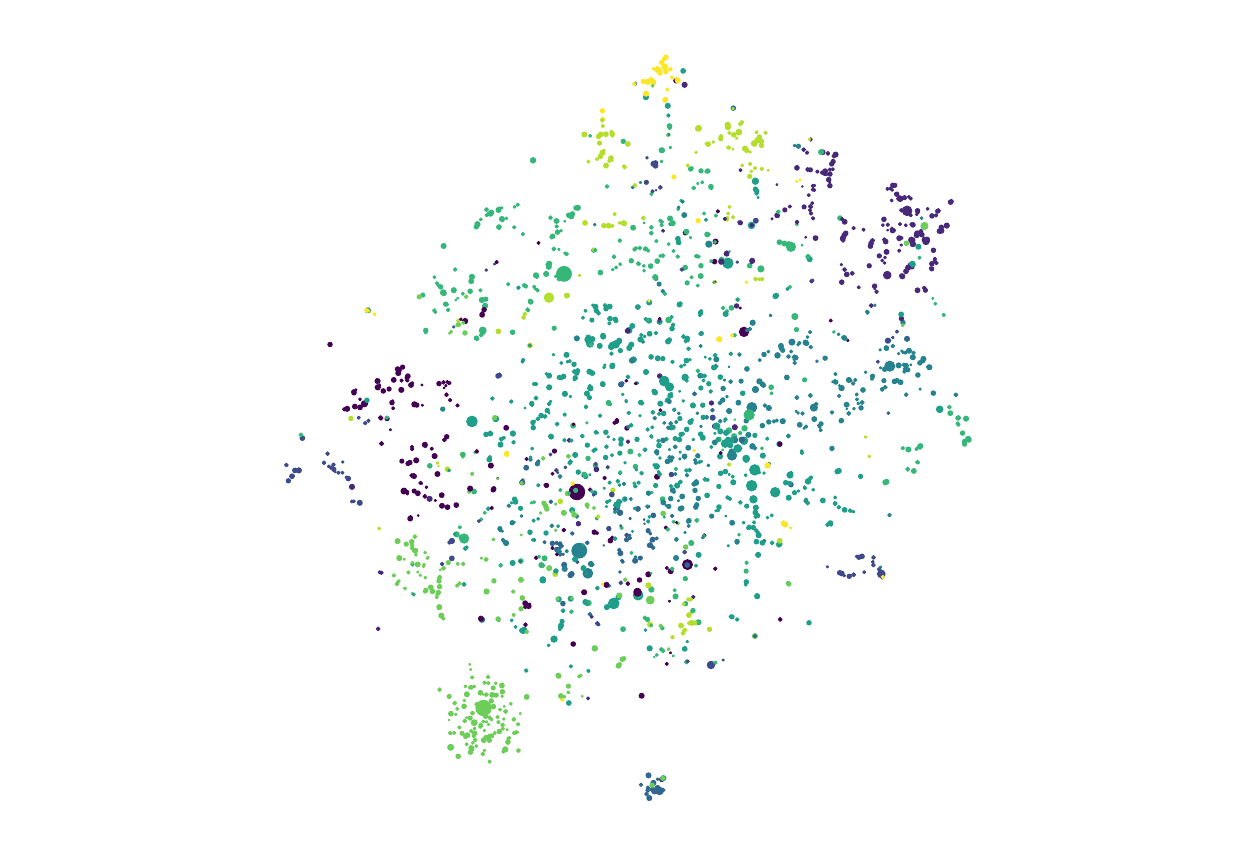
\begin{tikzpicture}[x=1pt,y=1pt]
\definecolor{fillColor}{RGB}{255,255,255}
\path[use as bounding box,fill=fillColor,fill opacity=0.00] (0,0) rectangle (433.62,289.08);
\begin{scope}
\path[clip] (  0.00,  0.00) rectangle (433.62,289.08);
\definecolor{drawColor}{RGB}{53,183,121}
\definecolor{fillColor}{RGB}{53,183,121}

\path[draw=drawColor,line width= 0.4pt,line join=round,line cap=round,fill=fillColor] (225.38, 86.05) circle (  0.92);
\definecolor{drawColor}{RGB}{31,158,137}
\definecolor{fillColor}{RGB}{31,158,137}

\path[draw=drawColor,line width= 0.4pt,line join=round,line cap=round,fill=fillColor] (223.40,263.95) circle (  0.89);
\definecolor{drawColor}{RGB}{53,183,121}
\definecolor{fillColor}{RGB}{53,183,121}

\path[draw=drawColor,line width= 0.4pt,line join=round,line cap=round,fill=fillColor] (234.10, 83.56) circle (  0.89);
\definecolor{drawColor}{RGB}{38,130,142}
\definecolor{fillColor}{RGB}{38,130,142}

\path[draw=drawColor,line width= 0.4pt,line join=round,line cap=round,fill=fillColor] (211.17, 80.75) circle (  0.89);
\definecolor{drawColor}{RGB}{109,205,89}
\definecolor{fillColor}{RGB}{109,205,89}

\path[draw=drawColor,line width= 0.4pt,line join=round,line cap=round,fill=fillColor] (224.97, 82.22) circle (  1.39);
\definecolor{drawColor}{RGB}{31,158,137}
\definecolor{fillColor}{RGB}{31,158,137}

\path[draw=drawColor,line width= 0.4pt,line join=round,line cap=round,fill=fillColor] (211.76, 81.02) circle (  1.90);

\path[draw=drawColor,line width= 0.4pt,line join=round,line cap=round,fill=fillColor] (270.21,192.07) circle (  0.89);

\path[draw=drawColor,line width= 0.4pt,line join=round,line cap=round,fill=fillColor] (220.61, 84.00) circle (  1.71);
\definecolor{drawColor}{RGB}{180,222,44}
\definecolor{fillColor}{RGB}{180,222,44}

\path[draw=drawColor,line width= 0.4pt,line join=round,line cap=round,fill=fillColor] (239.31, 82.29) circle (  0.43);
\definecolor{drawColor}{RGB}{72,40,120}
\definecolor{fillColor}{RGB}{72,40,120}

\path[draw=drawColor,line width= 0.4pt,line join=round,line cap=round,fill=fillColor] (291.93,243.22) circle (  0.89);
\definecolor{drawColor}{RGB}{31,158,137}
\definecolor{fillColor}{RGB}{31,158,137}

\path[draw=drawColor,line width= 0.4pt,line join=round,line cap=round,fill=fillColor] (261.61,123.57) circle (  1.86);
\definecolor{drawColor}{RGB}{53,183,121}
\definecolor{fillColor}{RGB}{53,183,121}

\path[draw=drawColor,line width= 0.4pt,line join=round,line cap=round,fill=fillColor] (150.30,210.20) circle (  0.89);
\definecolor{drawColor}{RGB}{180,222,44}
\definecolor{fillColor}{RGB}{180,222,44}

\path[draw=drawColor,line width= 0.4pt,line join=round,line cap=round,fill=fillColor] (224.31, 87.55) circle (  0.89);
\definecolor{drawColor}{RGB}{31,158,137}
\definecolor{fillColor}{RGB}{31,158,137}

\path[draw=drawColor,line width= 0.4pt,line join=round,line cap=round,fill=fillColor] (223.37,183.74) circle (  0.65);
\definecolor{drawColor}{RGB}{72,40,120}
\definecolor{fillColor}{RGB}{72,40,120}

\path[draw=drawColor,line width= 0.4pt,line join=round,line cap=round,fill=fillColor] (294.65,212.21) circle (  0.69);

\path[draw=drawColor,line width= 0.4pt,line join=round,line cap=round,fill=fillColor] (203.81, 76.22) circle (  0.53);
\definecolor{drawColor}{RGB}{253,231,37}
\definecolor{fillColor}{RGB}{253,231,37}

\path[draw=drawColor,line width= 0.4pt,line join=round,line cap=round,fill=fillColor] (226.11,269.41) circle (  0.89);
\definecolor{drawColor}{RGB}{31,158,137}
\definecolor{fillColor}{RGB}{31,158,137}

\path[draw=drawColor,line width= 0.4pt,line join=round,line cap=round,fill=fillColor] (214.17,172.38) circle (  0.72);
\definecolor{drawColor}{RGB}{49,104,142}
\definecolor{fillColor}{RGB}{49,104,142}

\path[draw=drawColor,line width= 0.4pt,line join=round,line cap=round,fill=fillColor] (224.34, 18.89) circle (  0.89);
\definecolor{drawColor}{RGB}{72,40,120}
\definecolor{fillColor}{RGB}{72,40,120}

\path[draw=drawColor,line width= 0.4pt,line join=round,line cap=round,fill=fillColor] (283.29,197.51) circle (  0.69);

\path[draw=drawColor,line width= 0.4pt,line join=round,line cap=round,fill=fillColor] (327.29,208.63) circle (  0.78);
\definecolor{drawColor}{RGB}{38,130,142}
\definecolor{fillColor}{RGB}{38,130,142}

\path[draw=drawColor,line width= 0.4pt,line join=round,line cap=round,fill=fillColor] (316.28,182.54) circle (  0.76);
\definecolor{drawColor}{RGB}{68,1,84}
\definecolor{fillColor}{RGB}{68,1,84}

\path[draw=drawColor,line width= 0.4pt,line join=round,line cap=round,fill=fillColor] (258.83,179.16) circle (  1.66);
\definecolor{drawColor}{RGB}{31,158,137}
\definecolor{fillColor}{RGB}{31,158,137}

\path[draw=drawColor,line width= 0.4pt,line join=round,line cap=round,fill=fillColor] (213.47, 83.28) circle (  0.89);
\definecolor{drawColor}{RGB}{72,40,120}
\definecolor{fillColor}{RGB}{72,40,120}

\path[draw=drawColor,line width= 0.4pt,line join=round,line cap=round,fill=fillColor] (240.51, 83.34) circle (  0.60);
\definecolor{drawColor}{RGB}{53,183,121}
\definecolor{fillColor}{RGB}{53,183,121}

\path[draw=drawColor,line width= 0.4pt,line join=round,line cap=round,fill=fillColor] (220.74, 83.90) circle (  0.89);
\definecolor{drawColor}{RGB}{31,158,137}
\definecolor{fillColor}{RGB}{31,158,137}

\path[draw=drawColor,line width= 0.4pt,line join=round,line cap=round,fill=fillColor] (174.88, 74.94) circle (  0.50);
\definecolor{drawColor}{RGB}{253,231,37}
\definecolor{fillColor}{RGB}{253,231,37}

\path[draw=drawColor,line width= 0.4pt,line join=round,line cap=round,fill=fillColor] (229.61,162.20) circle (  0.67);
\definecolor{drawColor}{RGB}{31,158,137}
\definecolor{fillColor}{RGB}{31,158,137}

\path[draw=drawColor,line width= 0.4pt,line join=round,line cap=round,fill=fillColor] (212.30,183.72) circle (  0.75);
\definecolor{drawColor}{RGB}{72,40,120}
\definecolor{fillColor}{RGB}{72,40,120}

\path[draw=drawColor,line width= 0.4pt,line join=round,line cap=round,fill=fillColor] (324.59,211.81) circle (  1.11);
\definecolor{drawColor}{RGB}{31,158,137}
\definecolor{fillColor}{RGB}{31,158,137}

\path[draw=drawColor,line width= 0.4pt,line join=round,line cap=round,fill=fillColor] (202.36,176.13) circle (  0.89);
\definecolor{drawColor}{RGB}{109,205,89}
\definecolor{fillColor}{RGB}{109,205,89}

\path[draw=drawColor,line width= 0.4pt,line join=round,line cap=round,fill=fillColor] (169.93, 75.27) circle (  0.61);
\definecolor{drawColor}{RGB}{53,183,121}
\definecolor{fillColor}{RGB}{53,183,121}

\path[draw=drawColor,line width= 0.4pt,line join=round,line cap=round,fill=fillColor] (260.89,203.06) circle (  0.80);
\definecolor{drawColor}{RGB}{72,40,120}
\definecolor{fillColor}{RGB}{72,40,120}

\path[draw=drawColor,line width= 0.4pt,line join=round,line cap=round,fill=fillColor] (319.52,202.68) circle (  0.80);
\definecolor{drawColor}{RGB}{31,158,137}
\definecolor{fillColor}{RGB}{31,158,137}

\path[draw=drawColor,line width= 0.4pt,line join=round,line cap=round,fill=fillColor] (220.46,188.13) circle (  0.82);

\path[draw=drawColor,line width= 0.4pt,line join=round,line cap=round,fill=fillColor] (196.22, 82.74) circle (  0.89);
\definecolor{drawColor}{RGB}{68,1,84}
\definecolor{fillColor}{RGB}{68,1,84}

\path[draw=drawColor,line width= 0.4pt,line join=round,line cap=round,fill=fillColor] (201.07, 85.07) circle (  0.89);

\path[draw=drawColor,line width= 0.4pt,line join=round,line cap=round,fill=fillColor] (220.41, 84.88) circle (  1.25);
\definecolor{drawColor}{RGB}{49,104,142}
\definecolor{fillColor}{RGB}{49,104,142}

\path[draw=drawColor,line width= 0.4pt,line join=round,line cap=round,fill=fillColor] (199.98, 99.91) circle (  0.42);
\definecolor{drawColor}{RGB}{53,183,121}
\definecolor{fillColor}{RGB}{53,183,121}

\path[draw=drawColor,line width= 0.4pt,line join=round,line cap=round,fill=fillColor] (188.91,220.42) circle (  0.66);

\path[draw=drawColor,line width= 0.4pt,line join=round,line cap=round,fill=fillColor] (255.47,147.45) circle (  0.26);
\definecolor{drawColor}{RGB}{31,158,137}
\definecolor{fillColor}{RGB}{31,158,137}

\path[draw=drawColor,line width= 0.4pt,line join=round,line cap=round,fill=fillColor] (210.87,173.76) circle (  1.01);
\definecolor{drawColor}{RGB}{38,130,142}
\definecolor{fillColor}{RGB}{38,130,142}

\path[draw=drawColor,line width= 0.4pt,line join=round,line cap=round,fill=fillColor] (323.68,169.39) circle (  0.89);
\definecolor{drawColor}{RGB}{72,40,120}
\definecolor{fillColor}{RGB}{72,40,120}

\path[draw=drawColor,line width= 0.4pt,line join=round,line cap=round,fill=fillColor] (315.72,183.99) circle (  0.77);
\definecolor{drawColor}{RGB}{53,183,121}
\definecolor{fillColor}{RGB}{53,183,121}

\path[draw=drawColor,line width= 0.4pt,line join=round,line cap=round,fill=fillColor] (230.24,192.94) circle (  0.64);
\definecolor{drawColor}{RGB}{31,158,137}
\definecolor{fillColor}{RGB}{31,158,137}

\path[draw=drawColor,line width= 0.4pt,line join=round,line cap=round,fill=fillColor] (174.75,153.98) circle (  0.63);
\definecolor{drawColor}{RGB}{109,205,89}
\definecolor{fillColor}{RGB}{109,205,89}

\path[draw=drawColor,line width= 0.4pt,line join=round,line cap=round,fill=fillColor] (180.31, 47.24) circle (  0.85);
\definecolor{drawColor}{RGB}{49,104,142}
\definecolor{fillColor}{RGB}{49,104,142}

\path[draw=drawColor,line width= 0.4pt,line join=round,line cap=round,fill=fillColor] (170.28, 74.95) circle (  0.43);

\path[draw=drawColor,line width= 0.4pt,line join=round,line cap=round,fill=fillColor] (196.56, 91.66) circle (  0.89);
\definecolor{drawColor}{RGB}{31,158,137}
\definecolor{fillColor}{RGB}{31,158,137}

\path[draw=drawColor,line width= 0.4pt,line join=round,line cap=round,fill=fillColor] (207.96,177.46) circle (  0.89);
\definecolor{drawColor}{RGB}{180,222,44}
\definecolor{fillColor}{RGB}{180,222,44}

\path[draw=drawColor,line width= 0.4pt,line join=round,line cap=round,fill=fillColor] (238.66, 82.52) circle (  0.59);
\definecolor{drawColor}{RGB}{31,158,137}
\definecolor{fillColor}{RGB}{31,158,137}

\path[draw=drawColor,line width= 0.4pt,line join=round,line cap=round,fill=fillColor] (262.74,129.28) circle (  1.86);
\definecolor{drawColor}{RGB}{253,231,37}
\definecolor{fillColor}{RGB}{253,231,37}

\path[draw=drawColor,line width= 0.4pt,line join=round,line cap=round,fill=fillColor] (230.38,263.01) circle (  0.89);
\definecolor{drawColor}{RGB}{68,1,84}
\definecolor{fillColor}{RGB}{68,1,84}

\path[draw=drawColor,line width= 0.4pt,line join=round,line cap=round,fill=fillColor] (118.23,152.16) circle (  0.84);
\definecolor{drawColor}{RGB}{31,158,137}
\definecolor{fillColor}{RGB}{31,158,137}

\path[draw=drawColor,line width= 0.4pt,line join=round,line cap=round,fill=fillColor] (231.30,260.84) circle (  0.89);
\definecolor{drawColor}{RGB}{180,222,44}
\definecolor{fillColor}{RGB}{180,222,44}

\path[draw=drawColor,line width= 0.4pt,line join=round,line cap=round,fill=fillColor] (266.63,251.09) circle (  0.59);
\definecolor{drawColor}{RGB}{31,158,137}
\definecolor{fillColor}{RGB}{31,158,137}

\path[draw=drawColor,line width= 0.4pt,line join=round,line cap=round,fill=fillColor] (209.29, 79.69) circle (  0.89);

\path[draw=drawColor,line width= 0.4pt,line join=round,line cap=round,fill=fillColor] (232.70,184.56) circle (  0.53);
\definecolor{drawColor}{RGB}{53,183,121}
\definecolor{fillColor}{RGB}{53,183,121}

\path[draw=drawColor,line width= 0.4pt,line join=round,line cap=round,fill=fillColor] (186.23, 94.74) circle (  0.68);
\definecolor{drawColor}{RGB}{109,205,89}
\definecolor{fillColor}{RGB}{109,205,89}

\path[draw=drawColor,line width= 0.4pt,line join=round,line cap=round,fill=fillColor] (316.15,181.56) circle (  0.51);
\definecolor{drawColor}{RGB}{53,183,121}
\definecolor{fillColor}{RGB}{53,183,121}

\path[draw=drawColor,line width= 0.4pt,line join=round,line cap=round,fill=fillColor] (264.93,201.91) circle (  1.09);
\definecolor{drawColor}{RGB}{109,205,89}
\definecolor{fillColor}{RGB}{109,205,89}

\path[draw=drawColor,line width= 0.4pt,line join=round,line cap=round,fill=fillColor] (195.40, 51.13) circle (  0.73);
\definecolor{drawColor}{RGB}{68,1,84}
\definecolor{fillColor}{RGB}{68,1,84}

\path[draw=drawColor,line width= 0.4pt,line join=round,line cap=round,fill=fillColor] (220.34, 85.23) circle (  1.28);

\path[draw=drawColor,line width= 0.4pt,line join=round,line cap=round,fill=fillColor] (231.92, 81.84) circle (  0.36);
\definecolor{drawColor}{RGB}{31,158,137}
\definecolor{fillColor}{RGB}{31,158,137}

\path[draw=drawColor,line width= 0.4pt,line join=round,line cap=round,fill=fillColor] (192.81, 73.16) circle (  0.81);
\definecolor{drawColor}{RGB}{72,40,120}
\definecolor{fillColor}{RGB}{72,40,120}

\path[draw=drawColor,line width= 0.4pt,line join=round,line cap=round,fill=fillColor] (283.79,220.19) circle (  0.59);
\definecolor{drawColor}{RGB}{253,231,37}
\definecolor{fillColor}{RGB}{253,231,37}

\path[draw=drawColor,line width= 0.4pt,line join=round,line cap=round,fill=fillColor] (223.45,265.23) circle (  0.89);
\definecolor{drawColor}{RGB}{72,40,120}
\definecolor{fillColor}{RGB}{72,40,120}

\path[draw=drawColor,line width= 0.4pt,line join=round,line cap=round,fill=fillColor] (254.03,204.66) circle (  0.53);
\definecolor{drawColor}{RGB}{53,183,121}
\definecolor{fillColor}{RGB}{53,183,121}

\path[draw=drawColor,line width= 0.4pt,line join=round,line cap=round,fill=fillColor] (211.85,206.32) circle (  0.67);
\definecolor{drawColor}{RGB}{68,1,84}
\definecolor{fillColor}{RGB}{68,1,84}

\path[draw=drawColor,line width= 0.4pt,line join=round,line cap=round,fill=fillColor] (127.46,148.16) circle (  0.71);
\definecolor{drawColor}{RGB}{53,183,121}
\definecolor{fillColor}{RGB}{53,183,121}

\path[draw=drawColor,line width= 0.4pt,line join=round,line cap=round,fill=fillColor] (322.26,205.92) circle (  0.56);
\definecolor{drawColor}{RGB}{109,205,89}
\definecolor{fillColor}{RGB}{109,205,89}

\path[draw=drawColor,line width= 0.4pt,line join=round,line cap=round,fill=fillColor] (204.93, 64.79) circle (  0.97);
\definecolor{drawColor}{RGB}{31,158,137}
\definecolor{fillColor}{RGB}{31,158,137}

\path[draw=drawColor,line width= 0.4pt,line join=round,line cap=round,fill=fillColor] (228.38,182.79) circle (  0.89);
\definecolor{drawColor}{RGB}{53,183,121}
\definecolor{fillColor}{RGB}{53,183,121}

\path[draw=drawColor,line width= 0.4pt,line join=round,line cap=round,fill=fillColor] (257.49,142.60) circle (  0.66);
\definecolor{drawColor}{RGB}{31,158,137}
\definecolor{fillColor}{RGB}{31,158,137}

\path[draw=drawColor,line width= 0.4pt,line join=round,line cap=round,fill=fillColor] (231.51,257.36) circle (  0.61);
\definecolor{drawColor}{RGB}{38,130,142}
\definecolor{fillColor}{RGB}{38,130,142}

\path[draw=drawColor,line width= 0.4pt,line join=round,line cap=round,fill=fillColor] (202.40, 91.92) circle (  1.73);
\definecolor{drawColor}{RGB}{53,183,121}
\definecolor{fillColor}{RGB}{53,183,121}

\path[draw=drawColor,line width= 0.4pt,line join=round,line cap=round,fill=fillColor] (259.05,144.30) circle (  0.95);
\definecolor{drawColor}{RGB}{38,130,142}
\definecolor{fillColor}{RGB}{38,130,142}

\path[draw=drawColor,line width= 0.4pt,line join=round,line cap=round,fill=fillColor] (267.83,151.64) circle (  0.89);
\definecolor{drawColor}{RGB}{180,222,44}
\definecolor{fillColor}{RGB}{180,222,44}

\path[draw=drawColor,line width= 0.4pt,line join=round,line cap=round,fill=fillColor] (202.64,240.65) circle (  0.56);
\definecolor{drawColor}{RGB}{38,130,142}
\definecolor{fillColor}{RGB}{38,130,142}

\path[draw=drawColor,line width= 0.4pt,line join=round,line cap=round,fill=fillColor] (323.44,168.69) circle (  0.73);
\definecolor{drawColor}{RGB}{31,158,137}
\definecolor{fillColor}{RGB}{31,158,137}

\path[draw=drawColor,line width= 0.4pt,line join=round,line cap=round,fill=fillColor] (160.54,146.78) circle (  1.90);
\definecolor{drawColor}{RGB}{38,130,142}
\definecolor{fillColor}{RGB}{38,130,142}

\path[draw=drawColor,line width= 0.4pt,line join=round,line cap=round,fill=fillColor] (315.42,160.95) circle (  0.84);
\definecolor{drawColor}{RGB}{68,1,84}
\definecolor{fillColor}{RGB}{68,1,84}

\path[draw=drawColor,line width= 0.4pt,line join=round,line cap=round,fill=fillColor] (216.86, 88.17) circle (  0.66);
\definecolor{drawColor}{RGB}{31,158,137}
\definecolor{fillColor}{RGB}{31,158,137}

\path[draw=drawColor,line width= 0.4pt,line join=round,line cap=round,fill=fillColor] (270.57,192.31) circle (  0.74);
\definecolor{drawColor}{RGB}{53,183,121}
\definecolor{fillColor}{RGB}{53,183,121}

\path[draw=drawColor,line width= 0.4pt,line join=round,line cap=round,fill=fillColor] (161.31,121.47) circle (  0.84);
\definecolor{drawColor}{RGB}{31,158,137}
\definecolor{fillColor}{RGB}{31,158,137}

\path[draw=drawColor,line width= 0.4pt,line join=round,line cap=round,fill=fillColor] (259.63,132.92) circle (  0.89);
\definecolor{drawColor}{RGB}{253,231,37}
\definecolor{fillColor}{RGB}{253,231,37}

\path[draw=drawColor,line width= 0.4pt,line join=round,line cap=round,fill=fillColor] (231.13,266.72) circle (  0.54);
\definecolor{drawColor}{RGB}{38,130,142}
\definecolor{fillColor}{RGB}{38,130,142}

\path[draw=drawColor,line width= 0.4pt,line join=round,line cap=round,fill=fillColor] (272.85,146.87) circle (  0.90);
\definecolor{drawColor}{RGB}{31,158,137}
\definecolor{fillColor}{RGB}{31,158,137}

\path[draw=drawColor,line width= 0.4pt,line join=round,line cap=round,fill=fillColor] (224.54,183.19) circle (  0.89);

\path[draw=drawColor,line width= 0.4pt,line join=round,line cap=round,fill=fillColor] (259.64,133.36) circle (  1.19);
\definecolor{drawColor}{RGB}{38,130,142}
\definecolor{fillColor}{RGB}{38,130,142}

\path[draw=drawColor,line width= 0.4pt,line join=round,line cap=round,fill=fillColor] (260.43,141.93) circle (  0.89);
\definecolor{drawColor}{RGB}{49,104,142}
\definecolor{fillColor}{RGB}{49,104,142}

\path[draw=drawColor,line width= 0.4pt,line join=round,line cap=round,fill=fillColor] (196.13, 91.24) circle (  0.89);
\definecolor{drawColor}{RGB}{31,158,137}
\definecolor{fillColor}{RGB}{31,158,137}

\path[draw=drawColor,line width= 0.4pt,line join=round,line cap=round,fill=fillColor] (267.24,140.55) circle (  0.58);
\definecolor{drawColor}{RGB}{53,183,121}
\definecolor{fillColor}{RGB}{53,183,121}

\path[draw=drawColor,line width= 0.4pt,line join=round,line cap=round,fill=fillColor] (280.73,161.83) circle (  0.73);
\definecolor{drawColor}{RGB}{31,158,137}
\definecolor{fillColor}{RGB}{31,158,137}

\path[draw=drawColor,line width= 0.4pt,line join=round,line cap=round,fill=fillColor] (253.00,203.99) circle (  1.85);

\path[draw=drawColor,line width= 0.4pt,line join=round,line cap=round,fill=fillColor] (203.19,174.84) circle (  1.22);
\definecolor{drawColor}{RGB}{253,231,37}
\definecolor{fillColor}{RGB}{253,231,37}

\path[draw=drawColor,line width= 0.4pt,line join=round,line cap=round,fill=fillColor] (249.21,176.39) circle (  0.43);

\path[draw=drawColor,line width= 0.4pt,line join=round,line cap=round,fill=fillColor] (223.91,269.50) circle (  0.89);
\definecolor{drawColor}{RGB}{72,40,120}
\definecolor{fillColor}{RGB}{72,40,120}

\path[draw=drawColor,line width= 0.4pt,line join=round,line cap=round,fill=fillColor] (291.05,240.70) circle (  0.75);
\definecolor{drawColor}{RGB}{68,1,84}
\definecolor{fillColor}{RGB}{68,1,84}

\path[draw=drawColor,line width= 0.4pt,line join=round,line cap=round,fill=fillColor] (138.79,127.27) circle (  0.69);
\definecolor{drawColor}{RGB}{31,158,137}
\definecolor{fillColor}{RGB}{31,158,137}

\path[draw=drawColor,line width= 0.4pt,line join=round,line cap=round,fill=fillColor] (218.12,174.52) circle (  0.89);

\path[draw=drawColor,line width= 0.4pt,line join=round,line cap=round,fill=fillColor] (205.85, 86.56) circle (  0.65);
\definecolor{drawColor}{RGB}{109,205,89}
\definecolor{fillColor}{RGB}{109,205,89}

\path[draw=drawColor,line width= 0.4pt,line join=round,line cap=round,fill=fillColor] (149.47, 76.62) circle (  0.89);
\definecolor{drawColor}{RGB}{72,40,120}
\definecolor{fillColor}{RGB}{72,40,120}

\path[draw=drawColor,line width= 0.4pt,line join=round,line cap=round,fill=fillColor] (329.52,215.57) circle (  0.85);
\definecolor{drawColor}{RGB}{180,222,44}
\definecolor{fillColor}{RGB}{180,222,44}

\path[draw=drawColor,line width= 0.4pt,line join=round,line cap=round,fill=fillColor] (207.06,250.49) circle (  0.84);
\definecolor{drawColor}{RGB}{53,183,121}
\definecolor{fillColor}{RGB}{53,183,121}

\path[draw=drawColor,line width= 0.4pt,line join=round,line cap=round,fill=fillColor] (202.74, 81.19) circle (  0.89);
\definecolor{drawColor}{RGB}{72,40,120}
\definecolor{fillColor}{RGB}{72,40,120}

\path[draw=drawColor,line width= 0.4pt,line join=round,line cap=round,fill=fillColor] (323.96,195.01) circle (  0.66);
\definecolor{drawColor}{RGB}{53,183,121}
\definecolor{fillColor}{RGB}{53,183,121}

\path[draw=drawColor,line width= 0.4pt,line join=round,line cap=round,fill=fillColor] (237.64, 89.98) circle (  0.75);
\definecolor{drawColor}{RGB}{38,130,142}
\definecolor{fillColor}{RGB}{38,130,142}

\path[draw=drawColor,line width= 0.4pt,line join=round,line cap=round,fill=fillColor] (325.85,166.37) circle (  0.89);
\definecolor{drawColor}{RGB}{31,158,137}
\definecolor{fillColor}{RGB}{31,158,137}

\path[draw=drawColor,line width= 0.4pt,line join=round,line cap=round,fill=fillColor] (210.86,174.85) circle (  0.53);
\definecolor{drawColor}{RGB}{180,222,44}
\definecolor{fillColor}{RGB}{180,222,44}

\path[draw=drawColor,line width= 0.4pt,line join=round,line cap=round,fill=fillColor] (239.69, 82.51) circle (  0.59);
\definecolor{drawColor}{RGB}{31,158,137}
\definecolor{fillColor}{RGB}{31,158,137}

\path[draw=drawColor,line width= 0.4pt,line join=round,line cap=round,fill=fillColor] (265.64,134.43) circle (  0.89);
\definecolor{drawColor}{RGB}{53,183,121}
\definecolor{fillColor}{RGB}{53,183,121}

\path[draw=drawColor,line width= 0.4pt,line join=round,line cap=round,fill=fillColor] (163.60,194.17) circle (  0.56);
\definecolor{drawColor}{RGB}{72,40,120}
\definecolor{fillColor}{RGB}{72,40,120}

\path[draw=drawColor,line width= 0.4pt,line join=round,line cap=round,fill=fillColor] (290.53,239.84) circle (  0.76);

\path[draw=drawColor,line width= 0.4pt,line join=round,line cap=round,fill=fillColor] (327.81,205.51) circle (  0.58);
\definecolor{drawColor}{RGB}{180,222,44}
\definecolor{fillColor}{RGB}{180,222,44}

\path[draw=drawColor,line width= 0.4pt,line join=round,line cap=round,fill=fillColor] (253.60,224.31) circle (  0.56);
\definecolor{drawColor}{RGB}{72,40,120}
\definecolor{fillColor}{RGB}{72,40,120}

\path[draw=drawColor,line width= 0.4pt,line join=round,line cap=round,fill=fillColor] (324.11,212.45) circle (  0.89);
\definecolor{drawColor}{RGB}{53,183,121}
\definecolor{fillColor}{RGB}{53,183,121}

\path[draw=drawColor,line width= 0.4pt,line join=round,line cap=round,fill=fillColor] (255.26,141.47) circle (  0.89);
\definecolor{drawColor}{RGB}{72,40,120}
\definecolor{fillColor}{RGB}{72,40,120}

\path[draw=drawColor,line width= 0.4pt,line join=round,line cap=round,fill=fillColor] (327.76,204.78) circle (  0.54);
\definecolor{drawColor}{RGB}{253,231,37}
\definecolor{fillColor}{RGB}{253,231,37}

\path[draw=drawColor,line width= 0.4pt,line join=round,line cap=round,fill=fillColor] (225.29,270.21) circle (  0.83);
\definecolor{drawColor}{RGB}{38,130,142}
\definecolor{fillColor}{RGB}{38,130,142}

\path[draw=drawColor,line width= 0.4pt,line join=round,line cap=round,fill=fillColor] (219.53,268.89) circle (  0.58);
\definecolor{drawColor}{RGB}{53,183,121}
\definecolor{fillColor}{RGB}{53,183,121}

\path[draw=drawColor,line width= 0.4pt,line join=round,line cap=round,fill=fillColor] (237.74, 80.93) circle (  0.76);
\definecolor{drawColor}{RGB}{180,222,44}
\definecolor{fillColor}{RGB}{180,222,44}

\path[draw=drawColor,line width= 0.4pt,line join=round,line cap=round,fill=fillColor] (236.96, 80.79) circle (  0.52);
\definecolor{drawColor}{RGB}{72,40,120}
\definecolor{fillColor}{RGB}{72,40,120}

\path[draw=drawColor,line width= 0.4pt,line join=round,line cap=round,fill=fillColor] (294.54,212.90) circle (  0.89);

\path[draw=drawColor,line width= 0.4pt,line join=round,line cap=round,fill=fillColor] (319.08,203.23) circle (  0.89);
\definecolor{drawColor}{RGB}{180,222,44}
\definecolor{fillColor}{RGB}{180,222,44}

\path[draw=drawColor,line width= 0.4pt,line join=round,line cap=round,fill=fillColor] (263.01,198.24) circle (  0.68);
\definecolor{drawColor}{RGB}{38,130,142}
\definecolor{fillColor}{RGB}{38,130,142}

\path[draw=drawColor,line width= 0.4pt,line join=round,line cap=round,fill=fillColor] (321.67,163.56) circle (  0.79);
\definecolor{drawColor}{RGB}{31,158,137}
\definecolor{fillColor}{RGB}{31,158,137}

\path[draw=drawColor,line width= 0.4pt,line join=round,line cap=round,fill=fillColor] (262.25,118.65) circle (  1.31);
\definecolor{drawColor}{RGB}{49,104,142}
\definecolor{fillColor}{RGB}{49,104,142}

\path[draw=drawColor,line width= 0.4pt,line join=round,line cap=round,fill=fillColor] (219.50, 96.45) circle (  0.89);
\definecolor{drawColor}{RGB}{72,40,120}
\definecolor{fillColor}{RGB}{72,40,120}

\path[draw=drawColor,line width= 0.4pt,line join=round,line cap=round,fill=fillColor] (319.40,218.00) circle (  0.68);

\path[draw=drawColor,line width= 0.4pt,line join=round,line cap=round,fill=fillColor] (313.32,232.10) circle (  0.74);
\definecolor{drawColor}{RGB}{180,222,44}
\definecolor{fillColor}{RGB}{180,222,44}

\path[draw=drawColor,line width= 0.4pt,line join=round,line cap=round,fill=fillColor] (256.59,190.85) circle (  0.62);

\path[draw=drawColor,line width= 0.4pt,line join=round,line cap=round,fill=fillColor] (211.26,250.68) circle (  0.78);
\definecolor{drawColor}{RGB}{31,158,137}
\definecolor{fillColor}{RGB}{31,158,137}

\path[draw=drawColor,line width= 0.4pt,line join=round,line cap=round,fill=fillColor] (253.09,140.21) circle (  0.89);

\path[draw=drawColor,line width= 0.4pt,line join=round,line cap=round,fill=fillColor] (201.96, 91.77) circle (  0.35);
\definecolor{drawColor}{RGB}{53,183,121}
\definecolor{fillColor}{RGB}{53,183,121}

\path[draw=drawColor,line width= 0.4pt,line join=round,line cap=round,fill=fillColor] (233.79, 85.81) circle (  0.53);
\definecolor{drawColor}{RGB}{180,222,44}
\definecolor{fillColor}{RGB}{180,222,44}

\path[draw=drawColor,line width= 0.4pt,line join=round,line cap=round,fill=fillColor] (242.60,252.62) circle (  0.60);

\path[draw=drawColor,line width= 0.4pt,line join=round,line cap=round,fill=fillColor] (238.52,239.26) circle (  0.56);
\definecolor{drawColor}{RGB}{72,40,120}
\definecolor{fillColor}{RGB}{72,40,120}

\path[draw=drawColor,line width= 0.4pt,line join=round,line cap=round,fill=fillColor] (321.25,214.12) circle (  0.91);
\definecolor{drawColor}{RGB}{109,205,89}
\definecolor{fillColor}{RGB}{109,205,89}

\path[draw=drawColor,line width= 0.4pt,line join=round,line cap=round,fill=fillColor] (324.05,217.42) circle (  1.26);
\definecolor{drawColor}{RGB}{31,158,137}
\definecolor{fillColor}{RGB}{31,158,137}

\path[draw=drawColor,line width= 0.4pt,line join=round,line cap=round,fill=fillColor] (217.34,179.74) circle (  1.02);
\definecolor{drawColor}{RGB}{53,183,121}
\definecolor{fillColor}{RGB}{53,183,121}

\path[draw=drawColor,line width= 0.4pt,line join=round,line cap=round,fill=fillColor] (203.59,174.48) circle (  0.59);
\definecolor{drawColor}{RGB}{253,231,37}
\definecolor{fillColor}{RGB}{253,231,37}

\path[draw=drawColor,line width= 0.4pt,line join=round,line cap=round,fill=fillColor] (273.14,109.97) circle (  0.89);
\definecolor{drawColor}{RGB}{109,205,89}
\definecolor{fillColor}{RGB}{109,205,89}

\path[draw=drawColor,line width= 0.4pt,line join=round,line cap=round,fill=fillColor] (225.83,268.05) circle (  0.52);
\definecolor{drawColor}{RGB}{68,1,84}
\definecolor{fillColor}{RGB}{68,1,84}

\path[draw=drawColor,line width= 0.4pt,line join=round,line cap=round,fill=fillColor] (179.85, 79.76) circle (  0.64);
\definecolor{drawColor}{RGB}{180,222,44}
\definecolor{fillColor}{RGB}{180,222,44}

\path[draw=drawColor,line width= 0.4pt,line join=round,line cap=round,fill=fillColor] (156.86,135.06) circle (  0.67);

\path[draw=drawColor,line width= 0.4pt,line join=round,line cap=round,fill=fillColor] (264.41,249.50) circle (  0.84);
\definecolor{drawColor}{RGB}{253,231,37}
\definecolor{fillColor}{RGB}{253,231,37}

\path[draw=drawColor,line width= 0.4pt,line join=round,line cap=round,fill=fillColor] (219.19,268.81) circle (  0.59);
\definecolor{drawColor}{RGB}{68,1,84}
\definecolor{fillColor}{RGB}{68,1,84}

\path[draw=drawColor,line width= 0.4pt,line join=round,line cap=round,fill=fillColor] (139.67,126.96) circle (  0.79);
\definecolor{drawColor}{RGB}{72,40,120}
\definecolor{fillColor}{RGB}{72,40,120}

\path[draw=drawColor,line width= 0.4pt,line join=round,line cap=round,fill=fillColor] (291.32,242.67) circle (  0.70);
\definecolor{drawColor}{RGB}{31,158,137}
\definecolor{fillColor}{RGB}{31,158,137}

\path[draw=drawColor,line width= 0.4pt,line join=round,line cap=round,fill=fillColor] (230.16,161.77) circle (  1.12);
\definecolor{drawColor}{RGB}{38,130,142}
\definecolor{fillColor}{RGB}{38,130,142}

\path[draw=drawColor,line width= 0.4pt,line join=round,line cap=round,fill=fillColor] (254.50,134.50) circle (  1.66);
\definecolor{drawColor}{RGB}{180,222,44}
\definecolor{fillColor}{RGB}{180,222,44}

\path[draw=drawColor,line width= 0.4pt,line join=round,line cap=round,fill=fillColor] (205.73,241.57) circle (  0.52);
\definecolor{drawColor}{RGB}{53,183,121}
\definecolor{fillColor}{RGB}{53,183,121}

\path[draw=drawColor,line width= 0.4pt,line join=round,line cap=round,fill=fillColor] (223.04, 75.81) circle (  0.68);
\definecolor{drawColor}{RGB}{31,158,137}
\definecolor{fillColor}{RGB}{31,158,137}

\path[draw=drawColor,line width= 0.4pt,line join=round,line cap=round,fill=fillColor] (210.14, 87.39) circle (  0.54);
\definecolor{drawColor}{RGB}{38,130,142}
\definecolor{fillColor}{RGB}{38,130,142}

\path[draw=drawColor,line width= 0.4pt,line join=round,line cap=round,fill=fillColor] (260.96,180.19) circle (  0.65);
\definecolor{drawColor}{RGB}{53,183,121}
\definecolor{fillColor}{RGB}{53,183,121}

\path[draw=drawColor,line width= 0.4pt,line join=round,line cap=round,fill=fillColor] (247.00,231.06) circle (  0.56);
\definecolor{drawColor}{RGB}{31,158,137}
\definecolor{fillColor}{RGB}{31,158,137}

\path[draw=drawColor,line width= 0.4pt,line join=round,line cap=round,fill=fillColor] (204.07,176.54) circle (  0.89);
\definecolor{drawColor}{RGB}{109,205,89}
\definecolor{fillColor}{RGB}{109,205,89}

\path[draw=drawColor,line width= 0.4pt,line join=round,line cap=round,fill=fillColor] (175.46, 85.32) circle (  0.62);
\definecolor{drawColor}{RGB}{49,104,142}
\definecolor{fillColor}{RGB}{49,104,142}

\path[draw=drawColor,line width= 0.4pt,line join=round,line cap=round,fill=fillColor] (193.86, 94.97) circle (  0.89);
\definecolor{drawColor}{RGB}{31,158,137}
\definecolor{fillColor}{RGB}{31,158,137}

\path[draw=drawColor,line width= 0.4pt,line join=round,line cap=round,fill=fillColor] (206.71,174.09) circle (  0.89);
\definecolor{drawColor}{RGB}{68,1,84}
\definecolor{fillColor}{RGB}{68,1,84}

\path[draw=drawColor,line width= 0.4pt,line join=round,line cap=round,fill=fillColor] (227.43,126.80) circle (  0.89);
\definecolor{drawColor}{RGB}{53,183,121}
\definecolor{fillColor}{RGB}{53,183,121}

\path[draw=drawColor,line width= 0.4pt,line join=round,line cap=round,fill=fillColor] (153.98,194.21) circle (  0.89);

\path[draw=drawColor,line width= 0.4pt,line join=round,line cap=round,fill=fillColor] (171.38,219.94) circle (  0.89);
\definecolor{drawColor}{RGB}{68,1,84}
\definecolor{fillColor}{RGB}{68,1,84}

\path[draw=drawColor,line width= 0.4pt,line join=round,line cap=round,fill=fillColor] (261.87,152.38) circle (  0.55);
\definecolor{drawColor}{RGB}{31,158,137}
\definecolor{fillColor}{RGB}{31,158,137}

\path[draw=drawColor,line width= 0.4pt,line join=round,line cap=round,fill=fillColor] (275.46,127.42) circle (  1.08);
\definecolor{drawColor}{RGB}{38,130,142}
\definecolor{fillColor}{RGB}{38,130,142}

\path[draw=drawColor,line width= 0.4pt,line join=round,line cap=round,fill=fillColor] (255.48,140.10) circle (  1.07);
\definecolor{drawColor}{RGB}{31,158,137}
\definecolor{fillColor}{RGB}{31,158,137}

\path[draw=drawColor,line width= 0.4pt,line join=round,line cap=round,fill=fillColor] (220.74,188.22) circle (  0.64);

\path[draw=drawColor,line width= 0.4pt,line join=round,line cap=round,fill=fillColor] (253.14,101.86) circle (  0.39);
\definecolor{drawColor}{RGB}{53,183,121}
\definecolor{fillColor}{RGB}{53,183,121}

\path[draw=drawColor,line width= 0.4pt,line join=round,line cap=round,fill=fillColor] (231.92,253.54) circle (  0.82);
\definecolor{drawColor}{RGB}{31,158,137}
\definecolor{fillColor}{RGB}{31,158,137}

\path[draw=drawColor,line width= 0.4pt,line join=round,line cap=round,fill=fillColor] (178.80,168.41) circle (  0.56);
\definecolor{drawColor}{RGB}{38,130,142}
\definecolor{fillColor}{RGB}{38,130,142}

\path[draw=drawColor,line width= 0.4pt,line join=round,line cap=round,fill=fillColor] (322.39,167.95) circle (  0.78);
\definecolor{drawColor}{RGB}{31,158,137}
\definecolor{fillColor}{RGB}{31,158,137}

\path[draw=drawColor,line width= 0.4pt,line join=round,line cap=round,fill=fillColor] (254.36,140.00) circle (  0.89);
\definecolor{drawColor}{RGB}{38,130,142}
\definecolor{fillColor}{RGB}{38,130,142}

\path[draw=drawColor,line width= 0.4pt,line join=round,line cap=round,fill=fillColor] (172.22,103.41) circle (  0.69);
\definecolor{drawColor}{RGB}{109,205,89}
\definecolor{fillColor}{RGB}{109,205,89}

\path[draw=drawColor,line width= 0.4pt,line join=round,line cap=round,fill=fillColor] (158.47,191.86) circle (  0.64);
\definecolor{drawColor}{RGB}{68,1,84}
\definecolor{fillColor}{RGB}{68,1,84}

\path[draw=drawColor,line width= 0.4pt,line join=round,line cap=round,fill=fillColor] (126.22,161.63) circle (  0.62);
\definecolor{drawColor}{RGB}{53,183,121}
\definecolor{fillColor}{RGB}{53,183,121}

\path[draw=drawColor,line width= 0.4pt,line join=round,line cap=round,fill=fillColor] (159.88,193.84) circle (  0.80);
\definecolor{drawColor}{RGB}{38,130,142}
\definecolor{fillColor}{RGB}{38,130,142}

\path[draw=drawColor,line width= 0.4pt,line join=round,line cap=round,fill=fillColor] (261.68,151.84) circle (  1.76);
\definecolor{drawColor}{RGB}{53,183,121}
\definecolor{fillColor}{RGB}{53,183,121}

\path[draw=drawColor,line width= 0.4pt,line join=round,line cap=round,fill=fillColor] (162.58,176.59) circle (  0.52);

\path[draw=drawColor,line width= 0.4pt,line join=round,line cap=round,fill=fillColor] (243.77,233.18) circle (  0.54);
\definecolor{drawColor}{RGB}{62,74,137}
\definecolor{fillColor}{RGB}{62,74,137}

\path[draw=drawColor,line width= 0.4pt,line join=round,line cap=round,fill=fillColor] (256.38,204.35) circle (  0.43);
\definecolor{drawColor}{RGB}{38,130,142}
\definecolor{fillColor}{RGB}{38,130,142}

\path[draw=drawColor,line width= 0.4pt,line join=round,line cap=round,fill=fillColor] (198.44,176.81) circle (  0.89);
\definecolor{drawColor}{RGB}{180,222,44}
\definecolor{fillColor}{RGB}{180,222,44}

\path[draw=drawColor,line width= 0.4pt,line join=round,line cap=round,fill=fillColor] (208.93,250.57) circle (  0.85);
\definecolor{drawColor}{RGB}{72,40,120}
\definecolor{fillColor}{RGB}{72,40,120}

\path[draw=drawColor,line width= 0.4pt,line join=round,line cap=round,fill=fillColor] (323.13,214.26) circle (  0.79);
\definecolor{drawColor}{RGB}{31,158,137}
\definecolor{fillColor}{RGB}{31,158,137}

\path[draw=drawColor,line width= 0.4pt,line join=round,line cap=round,fill=fillColor] (210.42,183.91) circle (  0.82);

\path[draw=drawColor,line width= 0.4pt,line join=round,line cap=round,fill=fillColor] (225.26,170.11) circle (  0.80);
\definecolor{drawColor}{RGB}{68,1,84}
\definecolor{fillColor}{RGB}{68,1,84}

\path[draw=drawColor,line width= 0.4pt,line join=round,line cap=round,fill=fillColor] (232.36, 92.67) circle (  0.89);
\definecolor{drawColor}{RGB}{62,74,137}
\definecolor{fillColor}{RGB}{62,74,137}

\path[draw=drawColor,line width= 0.4pt,line join=round,line cap=round,fill=fillColor] (247.55,148.15) circle (  0.89);
\definecolor{drawColor}{RGB}{68,1,84}
\definecolor{fillColor}{RGB}{68,1,84}

\path[draw=drawColor,line width= 0.4pt,line join=round,line cap=round,fill=fillColor] (221.09, 89.50) circle (  0.79);

\path[draw=drawColor,line width= 0.4pt,line join=round,line cap=round,fill=fillColor] (228.36,183.87) circle (  0.50);
\definecolor{drawColor}{RGB}{109,205,89}
\definecolor{fillColor}{RGB}{109,205,89}

\path[draw=drawColor,line width= 0.4pt,line join=round,line cap=round,fill=fillColor] (178.25, 79.08) circle (  0.73);
\definecolor{drawColor}{RGB}{180,222,44}
\definecolor{fillColor}{RGB}{180,222,44}

\path[draw=drawColor,line width= 0.4pt,line join=round,line cap=round,fill=fillColor] (263.37,251.27) circle (  0.56);
\definecolor{drawColor}{RGB}{72,40,120}
\definecolor{fillColor}{RGB}{72,40,120}

\path[draw=drawColor,line width= 0.4pt,line join=round,line cap=round,fill=fillColor] (324.92,212.36) circle (  1.02);
\definecolor{drawColor}{RGB}{31,158,137}
\definecolor{fillColor}{RGB}{31,158,137}

\path[draw=drawColor,line width= 0.4pt,line join=round,line cap=round,fill=fillColor] (227.69,169.61) circle (  0.89);
\definecolor{drawColor}{RGB}{68,1,84}
\definecolor{fillColor}{RGB}{68,1,84}

\path[draw=drawColor,line width= 0.4pt,line join=round,line cap=round,fill=fillColor] (133.91,164.28) circle (  0.89);
\definecolor{drawColor}{RGB}{38,130,142}
\definecolor{fillColor}{RGB}{38,130,142}

\path[draw=drawColor,line width= 0.4pt,line join=round,line cap=round,fill=fillColor] (194.06, 93.52) circle (  0.89);
\definecolor{drawColor}{RGB}{31,158,137}
\definecolor{fillColor}{RGB}{31,158,137}

\path[draw=drawColor,line width= 0.4pt,line join=round,line cap=round,fill=fillColor] (252.17,147.52) circle (  0.63);
\definecolor{drawColor}{RGB}{38,130,142}
\definecolor{fillColor}{RGB}{38,130,142}

\path[draw=drawColor,line width= 0.4pt,line join=round,line cap=round,fill=fillColor] (267.92,131.52) circle (  0.51);
\definecolor{drawColor}{RGB}{68,1,84}
\definecolor{fillColor}{RGB}{68,1,84}

\path[draw=drawColor,line width= 0.4pt,line join=round,line cap=round,fill=fillColor] (159.79,122.41) circle (  0.54);
\definecolor{drawColor}{RGB}{31,158,137}
\definecolor{fillColor}{RGB}{31,158,137}

\path[draw=drawColor,line width= 0.4pt,line join=round,line cap=round,fill=fillColor] (257.52,136.98) circle (  0.62);

\path[draw=drawColor,line width= 0.4pt,line join=round,line cap=round,fill=fillColor] (186.15, 89.46) circle (  1.04);
\definecolor{drawColor}{RGB}{68,1,84}
\definecolor{fillColor}{RGB}{68,1,84}

\path[draw=drawColor,line width= 0.4pt,line join=round,line cap=round,fill=fillColor] (127.68,147.97) circle (  0.70);
\definecolor{drawColor}{RGB}{72,40,120}
\definecolor{fillColor}{RGB}{72,40,120}

\path[draw=drawColor,line width= 0.4pt,line join=round,line cap=round,fill=fillColor] (319.35,212.35) circle (  1.01);
\definecolor{drawColor}{RGB}{31,158,137}
\definecolor{fillColor}{RGB}{31,158,137}

\path[draw=drawColor,line width= 0.4pt,line join=round,line cap=round,fill=fillColor] (269.01,102.91) circle (  0.70);
\definecolor{drawColor}{RGB}{53,183,121}
\definecolor{fillColor}{RGB}{53,183,121}

\path[draw=drawColor,line width= 0.4pt,line join=round,line cap=round,fill=fillColor] (165.29,188.55) circle (  0.92);

\path[draw=drawColor,line width= 0.4pt,line join=round,line cap=round,fill=fillColor] (239.52,213.23) circle (  0.41);
\definecolor{drawColor}{RGB}{49,104,142}
\definecolor{fillColor}{RGB}{49,104,142}

\path[draw=drawColor,line width= 0.4pt,line join=round,line cap=round,fill=fillColor] (164.15, 75.13) circle (  0.89);
\definecolor{drawColor}{RGB}{72,40,120}
\definecolor{fillColor}{RGB}{72,40,120}

\path[draw=drawColor,line width= 0.4pt,line join=round,line cap=round,fill=fillColor] (255.53,144.70) circle (  0.89);

\path[draw=drawColor,line width= 0.4pt,line join=round,line cap=round,fill=fillColor] (289.17,243.63) circle (  0.67);
\definecolor{drawColor}{RGB}{53,183,121}
\definecolor{fillColor}{RGB}{53,183,121}

\path[draw=drawColor,line width= 0.4pt,line join=round,line cap=round,fill=fillColor] (157.27,192.94) circle (  0.51);

\path[draw=drawColor,line width= 0.4pt,line join=round,line cap=round,fill=fillColor] (231.59,183.45) circle (  0.99);

\path[draw=drawColor,line width= 0.4pt,line join=round,line cap=round,fill=fillColor] (337.83,142.58) circle (  0.77);

\path[draw=drawColor,line width= 0.4pt,line join=round,line cap=round,fill=fillColor] (203.24,249.99) circle (  0.51);
\definecolor{drawColor}{RGB}{68,1,84}
\definecolor{fillColor}{RGB}{68,1,84}

\path[draw=drawColor,line width= 0.4pt,line join=round,line cap=round,fill=fillColor] (209.16, 87.72) circle (  0.89);
\definecolor{drawColor}{RGB}{109,205,89}
\definecolor{fillColor}{RGB}{109,205,89}

\path[draw=drawColor,line width= 0.4pt,line join=round,line cap=round,fill=fillColor] (213.80, 83.89) circle (  0.89);
\definecolor{drawColor}{RGB}{49,104,142}
\definecolor{fillColor}{RGB}{49,104,142}

\path[draw=drawColor,line width= 0.4pt,line join=round,line cap=round,fill=fillColor] (266.16,103.67) circle (  0.53);
\definecolor{drawColor}{RGB}{62,74,137}
\definecolor{fillColor}{RGB}{62,74,137}

\path[draw=drawColor,line width= 0.4pt,line join=round,line cap=round,fill=fillColor] (314.12,179.25) circle (  0.56);
\definecolor{drawColor}{RGB}{31,158,137}
\definecolor{fillColor}{RGB}{31,158,137}

\path[draw=drawColor,line width= 0.4pt,line join=round,line cap=round,fill=fillColor] (227.01,178.72) circle (  0.60);
\definecolor{drawColor}{RGB}{49,104,142}
\definecolor{fillColor}{RGB}{49,104,142}

\path[draw=drawColor,line width= 0.4pt,line join=round,line cap=round,fill=fillColor] (275.81,123.97) circle (  0.81);

\path[draw=drawColor,line width= 0.4pt,line join=round,line cap=round,fill=fillColor] (193.41, 80.98) circle (  0.79);
\definecolor{drawColor}{RGB}{31,158,137}
\definecolor{fillColor}{RGB}{31,158,137}

\path[draw=drawColor,line width= 0.4pt,line join=round,line cap=round,fill=fillColor] (202.98,164.77) circle (  0.89);

\path[draw=drawColor,line width= 0.4pt,line join=round,line cap=round,fill=fillColor] (240.39,152.57) circle (  0.89);

\path[draw=drawColor,line width= 0.4pt,line join=round,line cap=round,fill=fillColor] (229.69, 17.88) circle (  0.90);

\path[draw=drawColor,line width= 0.4pt,line join=round,line cap=round,fill=fillColor] (282.58,205.44) circle (  0.89);
\definecolor{drawColor}{RGB}{53,183,121}
\definecolor{fillColor}{RGB}{53,183,121}

\path[draw=drawColor,line width= 0.4pt,line join=round,line cap=round,fill=fillColor] (255.48,177.94) circle (  0.63);
\definecolor{drawColor}{RGB}{31,158,137}
\definecolor{fillColor}{RGB}{31,158,137}

\path[draw=drawColor,line width= 0.4pt,line join=round,line cap=round,fill=fillColor] (224.59,189.77) circle (  0.89);
\definecolor{drawColor}{RGB}{253,231,37}
\definecolor{fillColor}{RGB}{253,231,37}

\path[draw=drawColor,line width= 0.4pt,line join=round,line cap=round,fill=fillColor] (207.67, 88.03) circle (  0.40);
\definecolor{drawColor}{RGB}{180,222,44}
\definecolor{fillColor}{RGB}{180,222,44}

\path[draw=drawColor,line width= 0.4pt,line join=round,line cap=round,fill=fillColor] (190.65, 91.67) circle (  0.89);
\definecolor{drawColor}{RGB}{31,158,137}
\definecolor{fillColor}{RGB}{31,158,137}

\path[draw=drawColor,line width= 0.4pt,line join=round,line cap=round,fill=fillColor] (321.87,209.92) circle (  0.89);
\definecolor{drawColor}{RGB}{72,40,120}
\definecolor{fillColor}{RGB}{72,40,120}

\path[draw=drawColor,line width= 0.4pt,line join=round,line cap=round,fill=fillColor] (248.28,145.06) circle (  0.82);
\definecolor{drawColor}{RGB}{31,158,137}
\definecolor{fillColor}{RGB}{31,158,137}

\path[draw=drawColor,line width= 0.4pt,line join=round,line cap=round,fill=fillColor] (256.52,190.78) circle (  0.64);
\definecolor{drawColor}{RGB}{53,183,121}
\definecolor{fillColor}{RGB}{53,183,121}

\path[draw=drawColor,line width= 0.4pt,line join=round,line cap=round,fill=fillColor] (232.87, 93.52) circle (  0.68);

\path[draw=drawColor,line width= 0.4pt,line join=round,line cap=round,fill=fillColor] (253.38,143.50) circle (  0.98);
\definecolor{drawColor}{RGB}{38,130,142}
\definecolor{fillColor}{RGB}{38,130,142}

\path[draw=drawColor,line width= 0.4pt,line join=round,line cap=round,fill=fillColor] (222.36,175.53) circle (  0.49);
\definecolor{drawColor}{RGB}{31,158,137}
\definecolor{fillColor}{RGB}{31,158,137}

\path[draw=drawColor,line width= 0.4pt,line join=round,line cap=round,fill=fillColor] (315.62,185.49) circle (  0.84);
\definecolor{drawColor}{RGB}{72,40,120}
\definecolor{fillColor}{RGB}{72,40,120}

\path[draw=drawColor,line width= 0.4pt,line join=round,line cap=round,fill=fillColor] (117.19,123.16) circle (  0.90);
\definecolor{drawColor}{RGB}{62,74,137}
\definecolor{fillColor}{RGB}{62,74,137}

\path[draw=drawColor,line width= 0.4pt,line join=round,line cap=round,fill=fillColor] (237.42, 99.57) circle (  0.67);
\definecolor{drawColor}{RGB}{53,183,121}
\definecolor{fillColor}{RGB}{53,183,121}

\path[draw=drawColor,line width= 0.4pt,line join=round,line cap=round,fill=fillColor] (209.37,231.69) circle (  0.66);
\definecolor{drawColor}{RGB}{180,222,44}
\definecolor{fillColor}{RGB}{180,222,44}

\path[draw=drawColor,line width= 0.4pt,line join=round,line cap=round,fill=fillColor] (318.18,202.47) circle (  0.56);
\definecolor{drawColor}{RGB}{72,40,120}
\definecolor{fillColor}{RGB}{72,40,120}

\path[draw=drawColor,line width= 0.4pt,line join=round,line cap=round,fill=fillColor] (228.37,163.20) circle (  0.78);
\definecolor{drawColor}{RGB}{253,231,37}
\definecolor{fillColor}{RGB}{253,231,37}

\path[draw=drawColor,line width= 0.4pt,line join=round,line cap=round,fill=fillColor] (259.76,197.11) circle (  0.46);
\definecolor{drawColor}{RGB}{38,130,142}
\definecolor{fillColor}{RGB}{38,130,142}

\path[draw=drawColor,line width= 0.4pt,line join=round,line cap=round,fill=fillColor] (204.93,217.89) circle (  0.44);
\definecolor{drawColor}{RGB}{180,222,44}
\definecolor{fillColor}{RGB}{180,222,44}

\path[draw=drawColor,line width= 0.4pt,line join=round,line cap=round,fill=fillColor] (217.20,179.43) circle (  0.56);
\definecolor{drawColor}{RGB}{31,158,137}
\definecolor{fillColor}{RGB}{31,158,137}

\path[draw=drawColor,line width= 0.4pt,line join=round,line cap=round,fill=fillColor] (200.84, 93.79) circle (  0.88);
\definecolor{drawColor}{RGB}{38,130,142}
\definecolor{fillColor}{RGB}{38,130,142}

\path[draw=drawColor,line width= 0.4pt,line join=round,line cap=round,fill=fillColor] (323.00,220.26) circle (  0.49);
\definecolor{drawColor}{RGB}{72,40,120}
\definecolor{fillColor}{RGB}{72,40,120}

\path[draw=drawColor,line width= 0.4pt,line join=round,line cap=round,fill=fillColor] (256.17,188.53) circle (  0.76);
\definecolor{drawColor}{RGB}{68,1,84}
\definecolor{fillColor}{RGB}{68,1,84}

\path[draw=drawColor,line width= 0.4pt,line join=round,line cap=round,fill=fillColor] (296.33,176.11) circle (  0.43);
\definecolor{drawColor}{RGB}{38,130,142}
\definecolor{fillColor}{RGB}{38,130,142}

\path[draw=drawColor,line width= 0.4pt,line join=round,line cap=round,fill=fillColor] (259.63,147.01) circle (  0.77);
\definecolor{drawColor}{RGB}{53,183,121}
\definecolor{fillColor}{RGB}{53,183,121}

\path[draw=drawColor,line width= 0.4pt,line join=round,line cap=round,fill=fillColor] (271.46,102.28) circle (  0.89);
\definecolor{drawColor}{RGB}{31,158,137}
\definecolor{fillColor}{RGB}{31,158,137}

\path[draw=drawColor,line width= 0.4pt,line join=round,line cap=round,fill=fillColor] (230.00,161.39) circle (  1.72);
\definecolor{drawColor}{RGB}{53,183,121}
\definecolor{fillColor}{RGB}{53,183,121}

\path[draw=drawColor,line width= 0.4pt,line join=round,line cap=round,fill=fillColor] (260.70,149.17) circle (  1.83);
\definecolor{drawColor}{RGB}{49,104,142}
\definecolor{fillColor}{RGB}{49,104,142}

\path[draw=drawColor,line width= 0.4pt,line join=round,line cap=round,fill=fillColor] (317.75,176.64) circle (  0.89);
\definecolor{drawColor}{RGB}{72,40,120}
\definecolor{fillColor}{RGB}{72,40,120}

\path[draw=drawColor,line width= 0.4pt,line join=round,line cap=round,fill=fillColor] (271.62,102.40) circle (  0.54);
\definecolor{drawColor}{RGB}{31,158,137}
\definecolor{fillColor}{RGB}{31,158,137}

\path[draw=drawColor,line width= 0.4pt,line join=round,line cap=round,fill=fillColor] (319.68,203.60) circle (  1.05);
\definecolor{drawColor}{RGB}{72,40,120}
\definecolor{fillColor}{RGB}{72,40,120}

\path[draw=drawColor,line width= 0.4pt,line join=round,line cap=round,fill=fillColor] (229.11, 17.42) circle (  0.77);
\definecolor{drawColor}{RGB}{31,158,137}
\definecolor{fillColor}{RGB}{31,158,137}

\path[draw=drawColor,line width= 0.4pt,line join=round,line cap=round,fill=fillColor] (259.82,116.19) circle (  0.73);

\path[draw=drawColor,line width= 0.4pt,line join=round,line cap=round,fill=fillColor] (253.88,138.20) circle (  0.89);
\definecolor{drawColor}{RGB}{109,205,89}
\definecolor{fillColor}{RGB}{109,205,89}

\path[draw=drawColor,line width= 0.4pt,line join=round,line cap=round,fill=fillColor] (196.53, 82.91) circle (  0.45);

\path[draw=drawColor,line width= 0.4pt,line join=round,line cap=round,fill=fillColor] (215.91, 89.62) circle (  0.65);

\path[draw=drawColor,line width= 0.4pt,line join=round,line cap=round,fill=fillColor] (159.51,121.33) circle (  0.56);
\definecolor{drawColor}{RGB}{31,158,137}
\definecolor{fillColor}{RGB}{31,158,137}

\path[draw=drawColor,line width= 0.4pt,line join=round,line cap=round,fill=fillColor] (197.84,134.69) circle (  0.89);
\definecolor{drawColor}{RGB}{38,130,142}
\definecolor{fillColor}{RGB}{38,130,142}

\path[draw=drawColor,line width= 0.4pt,line join=round,line cap=round,fill=fillColor] (172.88,102.84) circle (  0.89);
\definecolor{drawColor}{RGB}{62,74,137}
\definecolor{fillColor}{RGB}{62,74,137}

\path[draw=drawColor,line width= 0.4pt,line join=round,line cap=round,fill=fillColor] (246.94, 58.93) circle (  0.51);
\definecolor{drawColor}{RGB}{31,158,137}
\definecolor{fillColor}{RGB}{31,158,137}

\path[draw=drawColor,line width= 0.4pt,line join=round,line cap=round,fill=fillColor] (218.96,169.15) circle (  0.98);

\path[draw=drawColor,line width= 0.4pt,line join=round,line cap=round,fill=fillColor] (275.01,119.21) circle (  0.89);
\definecolor{drawColor}{RGB}{72,40,120}
\definecolor{fillColor}{RGB}{72,40,120}

\path[draw=drawColor,line width= 0.4pt,line join=round,line cap=round,fill=fillColor] (319.84,212.29) circle (  0.78);
\definecolor{drawColor}{RGB}{31,158,137}
\definecolor{fillColor}{RGB}{31,158,137}

\path[draw=drawColor,line width= 0.4pt,line join=round,line cap=round,fill=fillColor] (253.23,150.63) circle (  0.63);

\path[draw=drawColor,line width= 0.4pt,line join=round,line cap=round,fill=fillColor] (191.91, 82.53) circle (  0.89);
\definecolor{drawColor}{RGB}{180,222,44}
\definecolor{fillColor}{RGB}{180,222,44}

\path[draw=drawColor,line width= 0.4pt,line join=round,line cap=round,fill=fillColor] (253.11,221.90) circle (  0.54);
\definecolor{drawColor}{RGB}{31,158,137}
\definecolor{fillColor}{RGB}{31,158,137}

\path[draw=drawColor,line width= 0.4pt,line join=round,line cap=round,fill=fillColor] (258.85,139.81) circle (  1.33);

\path[draw=drawColor,line width= 0.4pt,line join=round,line cap=round,fill=fillColor] (197.42,167.44) circle (  0.77);
\definecolor{drawColor}{RGB}{53,183,121}
\definecolor{fillColor}{RGB}{53,183,121}

\path[draw=drawColor,line width= 0.4pt,line join=round,line cap=round,fill=fillColor] (320.20,128.88) circle (  0.85);
\definecolor{drawColor}{RGB}{31,158,137}
\definecolor{fillColor}{RGB}{31,158,137}

\path[draw=drawColor,line width= 0.4pt,line join=round,line cap=round,fill=fillColor] (271.69,102.54) circle (  0.89);
\definecolor{drawColor}{RGB}{38,130,142}
\definecolor{fillColor}{RGB}{38,130,142}

\path[draw=drawColor,line width= 0.4pt,line join=round,line cap=round,fill=fillColor] (171.74,104.01) circle (  0.60);
\definecolor{drawColor}{RGB}{253,231,37}
\definecolor{fillColor}{RGB}{253,231,37}

\path[draw=drawColor,line width= 0.4pt,line join=round,line cap=round,fill=fillColor] (222.44,269.66) circle (  0.74);
\definecolor{drawColor}{RGB}{38,130,142}
\definecolor{fillColor}{RGB}{38,130,142}

\path[draw=drawColor,line width= 0.4pt,line join=round,line cap=round,fill=fillColor] (234.30, 97.44) circle (  0.89);

\path[draw=drawColor,line width= 0.4pt,line join=round,line cap=round,fill=fillColor] (254.37,135.94) circle (  0.89);
\definecolor{drawColor}{RGB}{68,1,84}
\definecolor{fillColor}{RGB}{68,1,84}

\path[draw=drawColor,line width= 0.4pt,line join=round,line cap=round,fill=fillColor] (238.42, 95.06) circle (  1.77);
\definecolor{drawColor}{RGB}{180,222,44}
\definecolor{fillColor}{RGB}{180,222,44}

\path[draw=drawColor,line width= 0.4pt,line join=round,line cap=round,fill=fillColor] (206.31,249.79) circle (  0.79);
\definecolor{drawColor}{RGB}{62,74,137}
\definecolor{fillColor}{RGB}{62,74,137}

\path[draw=drawColor,line width= 0.4pt,line join=round,line cap=round,fill=fillColor] (206.37, 73.35) circle (  0.44);
\definecolor{drawColor}{RGB}{31,158,137}
\definecolor{fillColor}{RGB}{31,158,137}

\path[draw=drawColor,line width= 0.4pt,line join=round,line cap=round,fill=fillColor] (252.04,138.79) circle (  1.36);
\definecolor{drawColor}{RGB}{38,130,142}
\definecolor{fillColor}{RGB}{38,130,142}

\path[draw=drawColor,line width= 0.4pt,line join=round,line cap=round,fill=fillColor] (266.40,152.54) circle (  0.63);

\path[draw=drawColor,line width= 0.4pt,line join=round,line cap=round,fill=fillColor] (319.85,169.99) circle (  0.89);
\definecolor{drawColor}{RGB}{68,1,84}
\definecolor{fillColor}{RGB}{68,1,84}

\path[draw=drawColor,line width= 0.4pt,line join=round,line cap=round,fill=fillColor] (138.09,131.96) circle (  0.78);
\definecolor{drawColor}{RGB}{62,74,137}
\definecolor{fillColor}{RGB}{62,74,137}

\path[draw=drawColor,line width= 0.4pt,line join=round,line cap=round,fill=fillColor] (312.62,177.15) circle (  0.44);
\definecolor{drawColor}{RGB}{180,222,44}
\definecolor{fillColor}{RGB}{180,222,44}

\path[draw=drawColor,line width= 0.4pt,line join=round,line cap=round,fill=fillColor] (207.08,242.43) circle (  0.69);
\definecolor{drawColor}{RGB}{253,231,37}
\definecolor{fillColor}{RGB}{253,231,37}

\path[draw=drawColor,line width= 0.4pt,line join=round,line cap=round,fill=fillColor] (125.36,185.55) circle (  0.53);
\definecolor{drawColor}{RGB}{38,130,142}
\definecolor{fillColor}{RGB}{38,130,142}

\path[draw=drawColor,line width= 0.4pt,line join=round,line cap=round,fill=fillColor] (269.64,146.80) circle (  0.61);
\definecolor{drawColor}{RGB}{62,74,137}
\definecolor{fillColor}{RGB}{62,74,137}

\path[draw=drawColor,line width= 0.4pt,line join=round,line cap=round,fill=fillColor] (283.65,197.76) circle (  0.46);
\definecolor{drawColor}{RGB}{53,183,121}
\definecolor{fillColor}{RGB}{53,183,121}

\path[draw=drawColor,line width= 0.4pt,line join=round,line cap=round,fill=fillColor] (175.79,216.96) circle (  0.58);
\definecolor{drawColor}{RGB}{68,1,84}
\definecolor{fillColor}{RGB}{68,1,84}

\path[draw=drawColor,line width= 0.4pt,line join=round,line cap=round,fill=fillColor] (159.87,122.54) circle (  0.89);
\definecolor{drawColor}{RGB}{31,158,137}
\definecolor{fillColor}{RGB}{31,158,137}

\path[draw=drawColor,line width= 0.4pt,line join=round,line cap=round,fill=fillColor] (231.96,159.26) circle (  1.43);
\definecolor{drawColor}{RGB}{72,40,120}
\definecolor{fillColor}{RGB}{72,40,120}

\path[draw=drawColor,line width= 0.4pt,line join=round,line cap=round,fill=fillColor] (321.42,214.67) circle (  0.96);
\definecolor{drawColor}{RGB}{31,158,137}
\definecolor{fillColor}{RGB}{31,158,137}

\path[draw=drawColor,line width= 0.4pt,line join=round,line cap=round,fill=fillColor] (232.21,156.14) circle (  0.89);
\definecolor{drawColor}{RGB}{62,74,137}
\definecolor{fillColor}{RGB}{62,74,137}

\path[draw=drawColor,line width= 0.4pt,line join=round,line cap=round,fill=fillColor] (228.23,183.04) circle (  0.46);
\definecolor{drawColor}{RGB}{72,40,120}
\definecolor{fillColor}{RGB}{72,40,120}

\path[draw=drawColor,line width= 0.4pt,line join=round,line cap=round,fill=fillColor] (318.13,202.36) circle (  0.89);
\definecolor{drawColor}{RGB}{109,205,89}
\definecolor{fillColor}{RGB}{109,205,89}

\path[draw=drawColor,line width= 0.4pt,line join=round,line cap=round,fill=fillColor] (262.80, 69.22) circle (  0.89);
\definecolor{drawColor}{RGB}{31,158,137}
\definecolor{fillColor}{RGB}{31,158,137}

\path[draw=drawColor,line width= 0.4pt,line join=round,line cap=round,fill=fillColor] (287.34,118.24) circle (  0.84);
\definecolor{drawColor}{RGB}{53,183,121}
\definecolor{fillColor}{RGB}{53,183,121}

\path[draw=drawColor,line width= 0.4pt,line join=round,line cap=round,fill=fillColor] (187.95,203.40) circle (  0.70);
\definecolor{drawColor}{RGB}{68,1,84}
\definecolor{fillColor}{RGB}{68,1,84}

\path[draw=drawColor,line width= 0.4pt,line join=round,line cap=round,fill=fillColor] (224.26, 91.54) circle (  0.89);
\definecolor{drawColor}{RGB}{31,158,137}
\definecolor{fillColor}{RGB}{31,158,137}

\path[draw=drawColor,line width= 0.4pt,line join=round,line cap=round,fill=fillColor] (193.10, 74.55) circle (  0.73);

\path[draw=drawColor,line width= 0.4pt,line join=round,line cap=round,fill=fillColor] (250.26,143.20) circle (  0.89);

\path[draw=drawColor,line width= 0.4pt,line join=round,line cap=round,fill=fillColor] (252.37,142.69) circle (  0.92);
\definecolor{drawColor}{RGB}{62,74,137}
\definecolor{fillColor}{RGB}{62,74,137}

\path[draw=drawColor,line width= 0.4pt,line join=round,line cap=round,fill=fillColor] (205.87, 73.79) circle (  0.70);

\path[draw=drawColor,line width= 0.4pt,line join=round,line cap=round,fill=fillColor] (149.77, 95.29) circle (  0.60);
\definecolor{drawColor}{RGB}{53,183,121}
\definecolor{fillColor}{RGB}{53,183,121}

\path[draw=drawColor,line width= 0.4pt,line join=round,line cap=round,fill=fillColor] (265.32,137.10) circle (  0.49);
\definecolor{drawColor}{RGB}{180,222,44}
\definecolor{fillColor}{RGB}{180,222,44}

\path[draw=drawColor,line width= 0.4pt,line join=round,line cap=round,fill=fillColor] (267.57,237.57) circle (  0.35);
\definecolor{drawColor}{RGB}{109,205,89}
\definecolor{fillColor}{RGB}{109,205,89}

\path[draw=drawColor,line width= 0.4pt,line join=round,line cap=round,fill=fillColor] (147.40,134.14) circle (  0.44);
\definecolor{drawColor}{RGB}{31,158,137}
\definecolor{fillColor}{RGB}{31,158,137}

\path[draw=drawColor,line width= 0.4pt,line join=round,line cap=round,fill=fillColor] (193.47, 78.39) circle (  0.71);
\definecolor{drawColor}{RGB}{109,205,89}
\definecolor{fillColor}{RGB}{109,205,89}

\path[draw=drawColor,line width= 0.4pt,line join=round,line cap=round,fill=fillColor] (136.79,102.47) circle (  0.74);
\definecolor{drawColor}{RGB}{31,158,137}
\definecolor{fillColor}{RGB}{31,158,137}

\path[draw=drawColor,line width= 0.4pt,line join=round,line cap=round,fill=fillColor] (217.23,179.71) circle (  0.71);
\definecolor{drawColor}{RGB}{49,104,142}
\definecolor{fillColor}{RGB}{49,104,142}

\path[draw=drawColor,line width= 0.4pt,line join=round,line cap=round,fill=fillColor] (215.03, 96.10) circle (  0.57);
\definecolor{drawColor}{RGB}{38,130,142}
\definecolor{fillColor}{RGB}{38,130,142}

\path[draw=drawColor,line width= 0.4pt,line join=round,line cap=round,fill=fillColor] (277.13,246.48) circle (  0.47);
\definecolor{drawColor}{RGB}{31,158,137}
\definecolor{fillColor}{RGB}{31,158,137}

\path[draw=drawColor,line width= 0.4pt,line join=round,line cap=round,fill=fillColor] (202.28,176.47) circle (  0.89);
\definecolor{drawColor}{RGB}{49,104,142}
\definecolor{fillColor}{RGB}{49,104,142}

\path[draw=drawColor,line width= 0.4pt,line join=round,line cap=round,fill=fillColor] (164.15, 75.20) circle (  0.89);
\definecolor{drawColor}{RGB}{62,74,137}
\definecolor{fillColor}{RGB}{62,74,137}

\path[draw=drawColor,line width= 0.4pt,line join=round,line cap=round,fill=fillColor] (108.28,135.33) circle (  0.41);
\definecolor{drawColor}{RGB}{253,231,37}
\definecolor{fillColor}{RGB}{253,231,37}

\path[draw=drawColor,line width= 0.4pt,line join=round,line cap=round,fill=fillColor] (226.17,274.23) circle (  0.54);
\definecolor{drawColor}{RGB}{68,1,84}
\definecolor{fillColor}{RGB}{68,1,84}

\path[draw=drawColor,line width= 0.4pt,line join=round,line cap=round,fill=fillColor] (164.93,187.18) circle (  0.78);
\definecolor{drawColor}{RGB}{253,231,37}
\definecolor{fillColor}{RGB}{253,231,37}

\path[draw=drawColor,line width= 0.4pt,line join=round,line cap=round,fill=fillColor] (228.48,272.66) circle (  0.75);
\definecolor{drawColor}{RGB}{31,158,137}
\definecolor{fillColor}{RGB}{31,158,137}

\path[draw=drawColor,line width= 0.4pt,line join=round,line cap=round,fill=fillColor] (226.68,157.26) circle (  0.89);
\definecolor{drawColor}{RGB}{49,104,142}
\definecolor{fillColor}{RGB}{49,104,142}

\path[draw=drawColor,line width= 0.4pt,line join=round,line cap=round,fill=fillColor] (214.75, 96.51) circle (  0.51);
\definecolor{drawColor}{RGB}{31,158,137}
\definecolor{fillColor}{RGB}{31,158,137}

\path[draw=drawColor,line width= 0.4pt,line join=round,line cap=round,fill=fillColor] (229.52,169.48) circle (  0.75);

\path[draw=drawColor,line width= 0.4pt,line join=round,line cap=round,fill=fillColor] (221.46,176.42) circle (  0.92);
\definecolor{drawColor}{RGB}{38,130,142}
\definecolor{fillColor}{RGB}{38,130,142}

\path[draw=drawColor,line width= 0.4pt,line join=round,line cap=round,fill=fillColor] (274.88,141.56) circle (  0.71);
\definecolor{drawColor}{RGB}{109,205,89}
\definecolor{fillColor}{RGB}{109,205,89}

\path[draw=drawColor,line width= 0.4pt,line join=round,line cap=round,fill=fillColor] (157.25,133.95) circle (  0.47);
\definecolor{drawColor}{RGB}{68,1,84}
\definecolor{fillColor}{RGB}{68,1,84}

\path[draw=drawColor,line width= 0.4pt,line join=round,line cap=round,fill=fillColor] (257.50,187.76) circle (  0.36);
\definecolor{drawColor}{RGB}{31,158,137}
\definecolor{fillColor}{RGB}{31,158,137}

\path[draw=drawColor,line width= 0.4pt,line join=round,line cap=round,fill=fillColor] (210.95,171.30) circle (  0.64);
\definecolor{drawColor}{RGB}{72,40,120}
\definecolor{fillColor}{RGB}{72,40,120}

\path[draw=drawColor,line width= 0.4pt,line join=round,line cap=round,fill=fillColor] (261.53,204.28) circle (  0.41);
\definecolor{drawColor}{RGB}{62,74,137}
\definecolor{fillColor}{RGB}{62,74,137}

\path[draw=drawColor,line width= 0.4pt,line join=round,line cap=round,fill=fillColor] (308.76, 90.57) circle (  0.70);
\definecolor{drawColor}{RGB}{109,205,89}
\definecolor{fillColor}{RGB}{109,205,89}

\path[draw=drawColor,line width= 0.4pt,line join=round,line cap=round,fill=fillColor] (138.77,103.33) circle (  0.77);

\path[draw=drawColor,line width= 0.4pt,line join=round,line cap=round,fill=fillColor] (188.44, 93.78) circle (  0.89);
\definecolor{drawColor}{RGB}{68,1,84}
\definecolor{fillColor}{RGB}{68,1,84}

\path[draw=drawColor,line width= 0.4pt,line join=round,line cap=round,fill=fillColor] (179.89, 73.36) circle (  0.66);
\definecolor{drawColor}{RGB}{38,130,142}
\definecolor{fillColor}{RGB}{38,130,142}

\path[draw=drawColor,line width= 0.4pt,line join=round,line cap=round,fill=fillColor] (271.63,138.64) circle (  0.89);
\definecolor{drawColor}{RGB}{72,40,120}
\definecolor{fillColor}{RGB}{72,40,120}

\path[draw=drawColor,line width= 0.4pt,line join=round,line cap=round,fill=fillColor] (328.34,204.07) circle (  0.65);
\definecolor{drawColor}{RGB}{31,158,137}
\definecolor{fillColor}{RGB}{31,158,137}

\path[draw=drawColor,line width= 0.4pt,line join=round,line cap=round,fill=fillColor] (211.34,167.08) circle (  0.80);
\definecolor{drawColor}{RGB}{180,222,44}
\definecolor{fillColor}{RGB}{180,222,44}

\path[draw=drawColor,line width= 0.4pt,line join=round,line cap=round,fill=fillColor] (264.38,198.15) circle (  0.53);
\definecolor{drawColor}{RGB}{31,158,137}
\definecolor{fillColor}{RGB}{31,158,137}

\path[draw=drawColor,line width= 0.4pt,line join=round,line cap=round,fill=fillColor] (187.75,150.73) circle (  0.78);

\path[draw=drawColor,line width= 0.4pt,line join=round,line cap=round,fill=fillColor] (256.57,137.03) circle (  1.34);
\definecolor{drawColor}{RGB}{72,40,120}
\definecolor{fillColor}{RGB}{72,40,120}

\path[draw=drawColor,line width= 0.4pt,line join=round,line cap=round,fill=fillColor] (317.38,201.06) circle (  0.83);
\definecolor{drawColor}{RGB}{31,158,137}
\definecolor{fillColor}{RGB}{31,158,137}

\path[draw=drawColor,line width= 0.4pt,line join=round,line cap=round,fill=fillColor] (194.71,170.86) circle (  0.89);
\definecolor{drawColor}{RGB}{72,40,120}
\definecolor{fillColor}{RGB}{72,40,120}

\path[draw=drawColor,line width= 0.4pt,line join=round,line cap=round,fill=fillColor] (330.13,216.96) circle (  0.78);
\definecolor{drawColor}{RGB}{53,183,121}
\definecolor{fillColor}{RGB}{53,183,121}

\path[draw=drawColor,line width= 0.4pt,line join=round,line cap=round,fill=fillColor] (231.96,252.80) circle (  0.56);

\path[draw=drawColor,line width= 0.4pt,line join=round,line cap=round,fill=fillColor] (162.67,217.95) circle (  0.72);
\definecolor{drawColor}{RGB}{180,222,44}
\definecolor{fillColor}{RGB}{180,222,44}

\path[draw=drawColor,line width= 0.4pt,line join=round,line cap=round,fill=fillColor] (241.93,252.37) circle (  0.62);
\definecolor{drawColor}{RGB}{31,158,137}
\definecolor{fillColor}{RGB}{31,158,137}

\path[draw=drawColor,line width= 0.4pt,line join=round,line cap=round,fill=fillColor] (202.58,177.18) circle (  0.82);
\definecolor{drawColor}{RGB}{68,1,84}
\definecolor{fillColor}{RGB}{68,1,84}

\path[draw=drawColor,line width= 0.4pt,line join=round,line cap=round,fill=fillColor] (147.32,118.23) circle (  0.38);
\definecolor{drawColor}{RGB}{31,158,137}
\definecolor{fillColor}{RGB}{31,158,137}

\path[draw=drawColor,line width= 0.4pt,line join=round,line cap=round,fill=fillColor] (201.99, 80.74) circle (  0.58);
\definecolor{drawColor}{RGB}{68,1,84}
\definecolor{fillColor}{RGB}{68,1,84}

\path[draw=drawColor,line width= 0.4pt,line join=round,line cap=round,fill=fillColor] (147.04,134.28) circle (  0.89);
\definecolor{drawColor}{RGB}{49,104,142}
\definecolor{fillColor}{RGB}{49,104,142}

\path[draw=drawColor,line width= 0.4pt,line join=round,line cap=round,fill=fillColor] (214.00, 92.39) circle (  0.44);
\definecolor{drawColor}{RGB}{253,231,37}
\definecolor{fillColor}{RGB}{253,231,37}

\path[draw=drawColor,line width= 0.4pt,line join=round,line cap=round,fill=fillColor] (249.96,176.50) circle (  0.89);
\definecolor{drawColor}{RGB}{53,183,121}
\definecolor{fillColor}{RGB}{53,183,121}

\path[draw=drawColor,line width= 0.4pt,line join=round,line cap=round,fill=fillColor] (251.11,136.49) circle (  0.31);
\definecolor{drawColor}{RGB}{31,158,137}
\definecolor{fillColor}{RGB}{31,158,137}

\path[draw=drawColor,line width= 0.4pt,line join=round,line cap=round,fill=fillColor] (259.46,133.16) circle (  0.65);
\definecolor{drawColor}{RGB}{53,183,121}
\definecolor{fillColor}{RGB}{53,183,121}

\path[draw=drawColor,line width= 0.4pt,line join=round,line cap=round,fill=fillColor] (193.80,200.11) circle (  2.65);
\definecolor{drawColor}{RGB}{38,130,142}
\definecolor{fillColor}{RGB}{38,130,142}

\path[draw=drawColor,line width= 0.4pt,line join=round,line cap=round,fill=fillColor] (228.17,196.42) circle (  0.72);

\path[draw=drawColor,line width= 0.4pt,line join=round,line cap=round,fill=fillColor] (270.70,147.12) circle (  0.55);
\definecolor{drawColor}{RGB}{53,183,121}
\definecolor{fillColor}{RGB}{53,183,121}

\path[draw=drawColor,line width= 0.4pt,line join=round,line cap=round,fill=fillColor] (229.15,244.85) circle (  0.49);
\definecolor{drawColor}{RGB}{180,222,44}
\definecolor{fillColor}{RGB}{180,222,44}

\path[draw=drawColor,line width= 0.4pt,line join=round,line cap=round,fill=fillColor] (207.18,250.53) circle (  0.52);
\definecolor{drawColor}{RGB}{31,158,137}
\definecolor{fillColor}{RGB}{31,158,137}

\path[draw=drawColor,line width= 0.4pt,line join=round,line cap=round,fill=fillColor] (210.19,182.23) circle (  0.60);
\definecolor{drawColor}{RGB}{49,104,142}
\definecolor{fillColor}{RGB}{49,104,142}

\path[draw=drawColor,line width= 0.4pt,line join=round,line cap=round,fill=fillColor] (247.45,150.85) circle (  0.63);
\definecolor{drawColor}{RGB}{31,158,137}
\definecolor{fillColor}{RGB}{31,158,137}

\path[draw=drawColor,line width= 0.4pt,line join=round,line cap=round,fill=fillColor] (232.62,157.04) circle (  0.31);
\definecolor{drawColor}{RGB}{49,104,142}
\definecolor{fillColor}{RGB}{49,104,142}

\path[draw=drawColor,line width= 0.4pt,line join=round,line cap=round,fill=fillColor] (227.61, 14.33) circle (  0.89);
\definecolor{drawColor}{RGB}{31,158,137}
\definecolor{fillColor}{RGB}{31,158,137}

\path[draw=drawColor,line width= 0.4pt,line join=round,line cap=round,fill=fillColor] (265.52,102.94) circle (  0.83);
\definecolor{drawColor}{RGB}{38,130,142}
\definecolor{fillColor}{RGB}{38,130,142}

\path[draw=drawColor,line width= 0.4pt,line join=round,line cap=round,fill=fillColor] (318.45,172.33) circle (  0.89);
\definecolor{drawColor}{RGB}{31,158,137}
\definecolor{fillColor}{RGB}{31,158,137}

\path[draw=drawColor,line width= 0.4pt,line join=round,line cap=round,fill=fillColor] (262.76,141.76) circle (  0.74);
\definecolor{drawColor}{RGB}{53,183,121}
\definecolor{fillColor}{RGB}{53,183,121}

\path[draw=drawColor,line width= 0.4pt,line join=round,line cap=round,fill=fillColor] (191.07,219.23) circle (  0.85);
\definecolor{drawColor}{RGB}{109,205,89}
\definecolor{fillColor}{RGB}{109,205,89}

\path[draw=drawColor,line width= 0.4pt,line join=round,line cap=round,fill=fillColor] (148.73, 79.70) circle (  0.89);
\definecolor{drawColor}{RGB}{253,231,37}
\definecolor{fillColor}{RGB}{253,231,37}

\path[draw=drawColor,line width= 0.4pt,line join=round,line cap=round,fill=fillColor] (273.80,109.54) circle (  0.89);
\definecolor{drawColor}{RGB}{31,158,137}
\definecolor{fillColor}{RGB}{31,158,137}

\path[draw=drawColor,line width= 0.4pt,line join=round,line cap=round,fill=fillColor] (212.56,183.24) circle (  0.73);

\path[draw=drawColor,line width= 0.4pt,line join=round,line cap=round,fill=fillColor] (329.55,151.17) circle (  1.16);
\definecolor{drawColor}{RGB}{253,231,37}
\definecolor{fillColor}{RGB}{253,231,37}

\path[draw=drawColor,line width= 0.4pt,line join=round,line cap=round,fill=fillColor] (123.73,186.42) circle (  0.37);
\definecolor{drawColor}{RGB}{53,183,121}
\definecolor{fillColor}{RGB}{53,183,121}

\path[draw=drawColor,line width= 0.4pt,line join=round,line cap=round,fill=fillColor] (280.65,161.96) circle (  0.46);
\definecolor{drawColor}{RGB}{72,40,120}
\definecolor{fillColor}{RGB}{72,40,120}

\path[draw=drawColor,line width= 0.4pt,line join=round,line cap=round,fill=fillColor] (322.82,215.57) circle (  0.70);
\definecolor{drawColor}{RGB}{109,205,89}
\definecolor{fillColor}{RGB}{109,205,89}

\path[draw=drawColor,line width= 0.4pt,line join=round,line cap=round,fill=fillColor] (133.66,103.55) circle (  0.89);
\definecolor{drawColor}{RGB}{31,158,137}
\definecolor{fillColor}{RGB}{31,158,137}

\path[draw=drawColor,line width= 0.4pt,line join=round,line cap=round,fill=fillColor] (208.53,167.15) circle (  0.40);
\definecolor{drawColor}{RGB}{53,183,121}
\definecolor{fillColor}{RGB}{53,183,121}

\path[draw=drawColor,line width= 0.4pt,line join=round,line cap=round,fill=fillColor] (195.54,221.29) circle (  0.82);
\definecolor{drawColor}{RGB}{31,158,137}
\definecolor{fillColor}{RGB}{31,158,137}

\path[draw=drawColor,line width= 0.4pt,line join=round,line cap=round,fill=fillColor] (277.09,121.04) circle (  0.72);
\definecolor{drawColor}{RGB}{53,183,121}
\definecolor{fillColor}{RGB}{53,183,121}

\path[draw=drawColor,line width= 0.4pt,line join=round,line cap=round,fill=fillColor] (246.89,231.60) circle (  0.82);
\definecolor{drawColor}{RGB}{68,1,84}
\definecolor{fillColor}{RGB}{68,1,84}

\path[draw=drawColor,line width= 0.4pt,line join=round,line cap=round,fill=fillColor] (139.52,127.62) circle (  0.38);
\definecolor{drawColor}{RGB}{31,158,137}
\definecolor{fillColor}{RGB}{31,158,137}

\path[draw=drawColor,line width= 0.4pt,line join=round,line cap=round,fill=fillColor] (208.30,166.34) circle (  0.51);
\definecolor{drawColor}{RGB}{68,1,84}
\definecolor{fillColor}{RGB}{68,1,84}

\path[draw=drawColor,line width= 0.4pt,line join=round,line cap=round,fill=fillColor] (115.46,151.35) circle (  0.89);
\definecolor{drawColor}{RGB}{53,183,121}
\definecolor{fillColor}{RGB}{53,183,121}

\path[draw=drawColor,line width= 0.4pt,line join=round,line cap=round,fill=fillColor] (157.28,134.79) circle (  0.81);
\definecolor{drawColor}{RGB}{109,205,89}
\definecolor{fillColor}{RGB}{109,205,89}

\path[draw=drawColor,line width= 0.4pt,line join=round,line cap=round,fill=fillColor] (175.62, 76.85) circle (  0.60);
\definecolor{drawColor}{RGB}{31,158,137}
\definecolor{fillColor}{RGB}{31,158,137}

\path[draw=drawColor,line width= 0.4pt,line join=round,line cap=round,fill=fillColor] (248.93,145.08) circle (  1.16);
\definecolor{drawColor}{RGB}{38,130,142}
\definecolor{fillColor}{RGB}{38,130,142}

\path[draw=drawColor,line width= 0.4pt,line join=round,line cap=round,fill=fillColor] (250.24,146.89) circle (  0.63);
\definecolor{drawColor}{RGB}{62,74,137}
\definecolor{fillColor}{RGB}{62,74,137}

\path[draw=drawColor,line width= 0.4pt,line join=round,line cap=round,fill=fillColor] (110.66,129.45) circle (  0.73);
\definecolor{drawColor}{RGB}{180,222,44}
\definecolor{fillColor}{RGB}{180,222,44}

\path[draw=drawColor,line width= 0.4pt,line join=round,line cap=round,fill=fillColor] (248.24,197.18) circle (  0.63);
\definecolor{drawColor}{RGB}{53,183,121}
\definecolor{fillColor}{RGB}{53,183,121}

\path[draw=drawColor,line width= 0.4pt,line join=round,line cap=round,fill=fillColor] (327.97,189.32) circle (  0.51);
\definecolor{drawColor}{RGB}{31,158,137}
\definecolor{fillColor}{RGB}{31,158,137}

\path[draw=drawColor,line width= 0.4pt,line join=round,line cap=round,fill=fillColor] (222.92,177.52) circle (  0.47);
\definecolor{drawColor}{RGB}{180,222,44}
\definecolor{fillColor}{RGB}{180,222,44}

\path[draw=drawColor,line width= 0.4pt,line join=round,line cap=round,fill=fillColor] (209.91,217.53) circle (  0.84);
\definecolor{drawColor}{RGB}{31,158,137}
\definecolor{fillColor}{RGB}{31,158,137}

\path[draw=drawColor,line width= 0.4pt,line join=round,line cap=round,fill=fillColor] (297.15,114.56) circle (  0.64);
\definecolor{drawColor}{RGB}{109,205,89}
\definecolor{fillColor}{RGB}{109,205,89}

\path[draw=drawColor,line width= 0.4pt,line join=round,line cap=round,fill=fillColor] (134.28, 97.42) circle (  0.90);
\definecolor{drawColor}{RGB}{72,40,120}
\definecolor{fillColor}{RGB}{72,40,120}

\path[draw=drawColor,line width= 0.4pt,line join=round,line cap=round,fill=fillColor] (312.51,231.62) circle (  0.51);

\path[draw=drawColor,line width= 0.4pt,line join=round,line cap=round,fill=fillColor] (295.05,214.05) circle (  0.82);
\definecolor{drawColor}{RGB}{68,1,84}
\definecolor{fillColor}{RGB}{68,1,84}

\path[draw=drawColor,line width= 0.4pt,line join=round,line cap=round,fill=fillColor] (140.40,132.74) circle (  0.89);
\definecolor{drawColor}{RGB}{253,231,37}
\definecolor{fillColor}{RGB}{253,231,37}

\path[draw=drawColor,line width= 0.4pt,line join=round,line cap=round,fill=fillColor] (224.43,269.22) circle (  0.64);
\definecolor{drawColor}{RGB}{49,104,142}
\definecolor{fillColor}{RGB}{49,104,142}

\path[draw=drawColor,line width= 0.4pt,line join=round,line cap=round,fill=fillColor] (229.62, 13.56) circle (  0.64);
\definecolor{drawColor}{RGB}{109,205,89}
\definecolor{fillColor}{RGB}{109,205,89}

\path[draw=drawColor,line width= 0.4pt,line join=round,line cap=round,fill=fillColor] (169.98, 75.39) circle (  0.79);
\definecolor{drawColor}{RGB}{38,130,142}
\definecolor{fillColor}{RGB}{38,130,142}

\path[draw=drawColor,line width= 0.4pt,line join=round,line cap=round,fill=fillColor] (262.75,137.18) circle (  0.68);
\definecolor{drawColor}{RGB}{31,158,137}
\definecolor{fillColor}{RGB}{31,158,137}

\path[draw=drawColor,line width= 0.4pt,line join=round,line cap=round,fill=fillColor] (279.76,135.43) circle (  0.62);
\definecolor{drawColor}{RGB}{180,222,44}
\definecolor{fillColor}{RGB}{180,222,44}

\path[draw=drawColor,line width= 0.4pt,line join=round,line cap=round,fill=fillColor] (271.77,103.66) circle (  0.82);
\definecolor{drawColor}{RGB}{31,158,137}
\definecolor{fillColor}{RGB}{31,158,137}

\path[draw=drawColor,line width= 0.4pt,line join=round,line cap=round,fill=fillColor] (263.95, 98.58) circle (  0.89);
\definecolor{drawColor}{RGB}{53,183,121}
\definecolor{fillColor}{RGB}{53,183,121}

\path[draw=drawColor,line width= 0.4pt,line join=round,line cap=round,fill=fillColor] (157.70,104.48) circle (  1.64);
\definecolor{drawColor}{RGB}{49,104,142}
\definecolor{fillColor}{RGB}{49,104,142}

\path[draw=drawColor,line width= 0.4pt,line join=round,line cap=round,fill=fillColor] (227.61, 17.52) circle (  0.46);
\definecolor{drawColor}{RGB}{31,158,137}
\definecolor{fillColor}{RGB}{31,158,137}

\path[draw=drawColor,line width= 0.4pt,line join=round,line cap=round,fill=fillColor] (207.88,177.84) circle (  0.79);
\definecolor{drawColor}{RGB}{72,40,120}
\definecolor{fillColor}{RGB}{72,40,120}

\path[draw=drawColor,line width= 0.4pt,line join=round,line cap=round,fill=fillColor] (282.92,248.64) circle (  0.61);
\definecolor{drawColor}{RGB}{62,74,137}
\definecolor{fillColor}{RGB}{62,74,137}

\path[draw=drawColor,line width= 0.4pt,line join=round,line cap=round,fill=fillColor] (302.31, 92.34) circle (  0.51);
\definecolor{drawColor}{RGB}{31,158,137}
\definecolor{fillColor}{RGB}{31,158,137}

\path[draw=drawColor,line width= 0.4pt,line join=round,line cap=round,fill=fillColor] (275.85,128.11) circle (  0.71);
\definecolor{drawColor}{RGB}{180,222,44}
\definecolor{fillColor}{RGB}{180,222,44}

\path[draw=drawColor,line width= 0.4pt,line join=round,line cap=round,fill=fillColor] (242.41,252.73) circle (  1.03);
\definecolor{drawColor}{RGB}{38,130,142}
\definecolor{fillColor}{RGB}{38,130,142}

\path[draw=drawColor,line width= 0.4pt,line join=round,line cap=round,fill=fillColor] (317.18,171.65) circle (  0.58);
\definecolor{drawColor}{RGB}{68,1,84}
\definecolor{fillColor}{RGB}{68,1,84}

\path[draw=drawColor,line width= 0.4pt,line join=round,line cap=round,fill=fillColor] (164.39,186.08) circle (  0.54);
\definecolor{drawColor}{RGB}{31,158,137}
\definecolor{fillColor}{RGB}{31,158,137}

\path[draw=drawColor,line width= 0.4pt,line join=round,line cap=round,fill=fillColor] (291.76,119.32) circle (  0.52);

\path[draw=drawColor,line width= 0.4pt,line join=round,line cap=round,fill=fillColor] (268.86,112.86) circle (  0.55);
\definecolor{drawColor}{RGB}{38,130,142}
\definecolor{fillColor}{RGB}{38,130,142}

\path[draw=drawColor,line width= 0.4pt,line join=round,line cap=round,fill=fillColor] (262.97,158.32) circle (  1.08);

\path[draw=drawColor,line width= 0.4pt,line join=round,line cap=round,fill=fillColor] (259.89,179.72) circle (  0.56);
\definecolor{drawColor}{RGB}{72,40,120}
\definecolor{fillColor}{RGB}{72,40,120}

\path[draw=drawColor,line width= 0.4pt,line join=round,line cap=round,fill=fillColor] (330.17,215.70) circle (  0.89);
\definecolor{drawColor}{RGB}{53,183,121}
\definecolor{fillColor}{RGB}{53,183,121}

\path[draw=drawColor,line width= 0.4pt,line join=round,line cap=round,fill=fillColor] (249.75,140.30) circle (  0.83);
\definecolor{drawColor}{RGB}{72,40,120}
\definecolor{fillColor}{RGB}{72,40,120}

\path[draw=drawColor,line width= 0.4pt,line join=round,line cap=round,fill=fillColor] (290.96,237.90) circle (  0.52);
\definecolor{drawColor}{RGB}{38,130,142}
\definecolor{fillColor}{RGB}{38,130,142}

\path[draw=drawColor,line width= 0.4pt,line join=round,line cap=round,fill=fillColor] (301.14,151.68) circle (  0.78);
\definecolor{drawColor}{RGB}{31,158,137}
\definecolor{fillColor}{RGB}{31,158,137}

\path[draw=drawColor,line width= 0.4pt,line join=round,line cap=round,fill=fillColor] (250.19,134.15) circle (  0.89);
\definecolor{drawColor}{RGB}{72,40,120}
\definecolor{fillColor}{RGB}{72,40,120}

\path[draw=drawColor,line width= 0.4pt,line join=round,line cap=round,fill=fillColor] (247.35, 59.16) circle (  0.61);
\definecolor{drawColor}{RGB}{68,1,84}
\definecolor{fillColor}{RGB}{68,1,84}

\path[draw=drawColor,line width= 0.4pt,line join=round,line cap=round,fill=fillColor] (150.48,158.89) circle (  0.31);
\definecolor{drawColor}{RGB}{53,183,121}
\definecolor{fillColor}{RGB}{53,183,121}

\path[draw=drawColor,line width= 0.4pt,line join=round,line cap=round,fill=fillColor] (198.82,223.99) circle (  0.89);
\definecolor{drawColor}{RGB}{62,74,137}
\definecolor{fillColor}{RGB}{62,74,137}

\path[draw=drawColor,line width= 0.4pt,line join=round,line cap=round,fill=fillColor] (308.25, 92.10) circle (  0.56);
\definecolor{drawColor}{RGB}{38,130,142}
\definecolor{fillColor}{RGB}{38,130,142}

\path[draw=drawColor,line width= 0.4pt,line join=round,line cap=round,fill=fillColor] (301.55,153.65) circle (  0.71);
\definecolor{drawColor}{RGB}{72,40,120}
\definecolor{fillColor}{RGB}{72,40,120}

\path[draw=drawColor,line width= 0.4pt,line join=round,line cap=round,fill=fillColor] (321.54,194.18) circle (  0.84);
\definecolor{drawColor}{RGB}{49,104,142}
\definecolor{fillColor}{RGB}{49,104,142}

\path[draw=drawColor,line width= 0.4pt,line join=round,line cap=round,fill=fillColor] (225.79, 15.08) circle (  0.48);
\definecolor{drawColor}{RGB}{53,183,121}
\definecolor{fillColor}{RGB}{53,183,121}

\path[draw=drawColor,line width= 0.4pt,line join=round,line cap=round,fill=fillColor] (156.78,104.89) circle (  0.89);
\definecolor{drawColor}{RGB}{72,40,120}
\definecolor{fillColor}{RGB}{72,40,120}

\path[draw=drawColor,line width= 0.4pt,line join=round,line cap=round,fill=fillColor] (317.31,217.68) circle (  0.51);
\definecolor{drawColor}{RGB}{31,158,137}
\definecolor{fillColor}{RGB}{31,158,137}

\path[draw=drawColor,line width= 0.4pt,line join=round,line cap=round,fill=fillColor] (311.52,176.14) circle (  0.40);

\path[draw=drawColor,line width= 0.4pt,line join=round,line cap=round,fill=fillColor] (264.41,128.31) circle (  0.43);
\definecolor{drawColor}{RGB}{62,74,137}
\definecolor{fillColor}{RGB}{62,74,137}

\path[draw=drawColor,line width= 0.4pt,line join=round,line cap=round,fill=fillColor] (310.84,175.96) circle (  0.89);
\definecolor{drawColor}{RGB}{53,183,121}
\definecolor{fillColor}{RGB}{53,183,121}

\path[draw=drawColor,line width= 0.4pt,line join=round,line cap=round,fill=fillColor] (225.26, 91.96) circle (  0.33);
\definecolor{drawColor}{RGB}{31,158,137}
\definecolor{fillColor}{RGB}{31,158,137}

\path[draw=drawColor,line width= 0.4pt,line join=round,line cap=round,fill=fillColor] (251.85,146.87) circle (  0.34);
\definecolor{drawColor}{RGB}{68,1,84}
\definecolor{fillColor}{RGB}{68,1,84}

\path[draw=drawColor,line width= 0.4pt,line join=round,line cap=round,fill=fillColor] (126.44,161.37) circle (  0.89);
\definecolor{drawColor}{RGB}{31,158,137}
\definecolor{fillColor}{RGB}{31,158,137}

\path[draw=drawColor,line width= 0.4pt,line join=round,line cap=round,fill=fillColor] (198.42,164.23) circle (  0.75);
\definecolor{drawColor}{RGB}{68,1,84}
\definecolor{fillColor}{RGB}{68,1,84}

\path[draw=drawColor,line width= 0.4pt,line join=round,line cap=round,fill=fillColor] (132.28,161.79) circle (  0.84);
\definecolor{drawColor}{RGB}{72,40,120}
\definecolor{fillColor}{RGB}{72,40,120}

\path[draw=drawColor,line width= 0.4pt,line join=round,line cap=round,fill=fillColor] (328.24,221.25) circle (  0.60);
\definecolor{drawColor}{RGB}{49,104,142}
\definecolor{fillColor}{RGB}{49,104,142}

\path[draw=drawColor,line width= 0.4pt,line join=round,line cap=round,fill=fillColor] (226.11, 16.18) circle (  0.89);
\definecolor{drawColor}{RGB}{31,158,137}
\definecolor{fillColor}{RGB}{31,158,137}

\path[draw=drawColor,line width= 0.4pt,line join=round,line cap=round,fill=fillColor] (232.84,180.34) circle (  0.80);
\definecolor{drawColor}{RGB}{180,222,44}
\definecolor{fillColor}{RGB}{180,222,44}

\path[draw=drawColor,line width= 0.4pt,line join=round,line cap=round,fill=fillColor] (238.91, 76.78) circle (  0.82);

\path[draw=drawColor,line width= 0.4pt,line join=round,line cap=round,fill=fillColor] (207.70,243.92) circle (  0.89);
\definecolor{drawColor}{RGB}{38,130,142}
\definecolor{fillColor}{RGB}{38,130,142}

\path[draw=drawColor,line width= 0.4pt,line join=round,line cap=round,fill=fillColor] (265.48,145.28) circle (  0.79);
\definecolor{drawColor}{RGB}{31,158,137}
\definecolor{fillColor}{RGB}{31,158,137}

\path[draw=drawColor,line width= 0.4pt,line join=round,line cap=round,fill=fillColor] (243.86,140.90) circle (  0.47);
\definecolor{drawColor}{RGB}{49,104,142}
\definecolor{fillColor}{RGB}{49,104,142}

\path[draw=drawColor,line width= 0.4pt,line join=round,line cap=round,fill=fillColor] (225.77, 16.03) circle (  0.52);
\definecolor{drawColor}{RGB}{53,183,121}
\definecolor{fillColor}{RGB}{53,183,121}

\path[draw=drawColor,line width= 0.4pt,line join=round,line cap=round,fill=fillColor] (243.21,199.32) circle (  0.87);
\definecolor{drawColor}{RGB}{49,104,142}
\definecolor{fillColor}{RGB}{49,104,142}

\path[draw=drawColor,line width= 0.4pt,line join=round,line cap=round,fill=fillColor] (192.43, 98.74) circle (  0.65);
\definecolor{drawColor}{RGB}{31,158,137}
\definecolor{fillColor}{RGB}{31,158,137}

\path[draw=drawColor,line width= 0.4pt,line join=round,line cap=round,fill=fillColor] (122.91,186.97) circle (  0.89);
\definecolor{drawColor}{RGB}{62,74,137}
\definecolor{fillColor}{RGB}{62,74,137}

\path[draw=drawColor,line width= 0.4pt,line join=round,line cap=round,fill=fillColor] (308.44, 91.70) circle (  1.36);
\definecolor{drawColor}{RGB}{72,40,120}
\definecolor{fillColor}{RGB}{72,40,120}

\path[draw=drawColor,line width= 0.4pt,line join=round,line cap=round,fill=fillColor] (289.88,237.80) circle (  0.58);

\path[draw=drawColor,line width= 0.4pt,line join=round,line cap=round,fill=fillColor] (326.71,203.76) circle (  0.78);
\definecolor{drawColor}{RGB}{49,104,142}
\definecolor{fillColor}{RGB}{49,104,142}

\path[draw=drawColor,line width= 0.4pt,line join=round,line cap=round,fill=fillColor] (224.61, 10.71) circle (  0.89);
\definecolor{drawColor}{RGB}{38,130,142}
\definecolor{fillColor}{RGB}{38,130,142}

\path[draw=drawColor,line width= 0.4pt,line join=round,line cap=round,fill=fillColor] (314.14,161.55) circle (  0.75);
\definecolor{drawColor}{RGB}{53,183,121}
\definecolor{fillColor}{RGB}{53,183,121}

\path[draw=drawColor,line width= 0.4pt,line join=round,line cap=round,fill=fillColor] (160.27,197.45) circle (  0.85);

\path[draw=drawColor,line width= 0.4pt,line join=round,line cap=round,fill=fillColor] (165.55,190.97) circle (  0.75);
\definecolor{drawColor}{RGB}{38,130,142}
\definecolor{fillColor}{RGB}{38,130,142}

\path[draw=drawColor,line width= 0.4pt,line join=round,line cap=round,fill=fillColor] (265.86,159.89) circle (  0.76);
\definecolor{drawColor}{RGB}{49,104,142}
\definecolor{fillColor}{RGB}{49,104,142}

\path[draw=drawColor,line width= 0.4pt,line join=round,line cap=round,fill=fillColor] (224.14, 14.41) circle (  0.64);
\definecolor{drawColor}{RGB}{31,158,137}
\definecolor{fillColor}{RGB}{31,158,137}

\path[draw=drawColor,line width= 0.4pt,line join=round,line cap=round,fill=fillColor] (226.32,157.71) circle (  0.73);
\definecolor{drawColor}{RGB}{62,74,137}
\definecolor{fillColor}{RGB}{62,74,137}

\path[draw=drawColor,line width= 0.4pt,line join=round,line cap=round,fill=fillColor] (214.32, 88.47) circle (  0.65);
\definecolor{drawColor}{RGB}{72,40,120}
\definecolor{fillColor}{RGB}{72,40,120}

\path[draw=drawColor,line width= 0.4pt,line join=round,line cap=round,fill=fillColor] (127.82, 92.12) circle (  0.64);
\definecolor{drawColor}{RGB}{31,158,137}
\definecolor{fillColor}{RGB}{31,158,137}

\path[draw=drawColor,line width= 0.4pt,line join=round,line cap=round,fill=fillColor] (183.15,146.90) circle (  0.37);
\definecolor{drawColor}{RGB}{62,74,137}
\definecolor{fillColor}{RGB}{62,74,137}

\path[draw=drawColor,line width= 0.4pt,line join=round,line cap=round,fill=fillColor] ( 99.26,140.76) circle (  0.81);
\definecolor{drawColor}{RGB}{180,222,44}
\definecolor{fillColor}{RGB}{180,222,44}

\path[draw=drawColor,line width= 0.4pt,line join=round,line cap=round,fill=fillColor] (239.73, 77.65) circle (  0.50);
\definecolor{drawColor}{RGB}{53,183,121}
\definecolor{fillColor}{RGB}{53,183,121}

\path[draw=drawColor,line width= 0.4pt,line join=round,line cap=round,fill=fillColor] (182.62,241.13) circle (  0.89);
\definecolor{drawColor}{RGB}{31,158,137}
\definecolor{fillColor}{RGB}{31,158,137}

\path[draw=drawColor,line width= 0.4pt,line join=round,line cap=round,fill=fillColor] (190.88, 92.75) circle (  0.79);
\definecolor{drawColor}{RGB}{38,130,142}
\definecolor{fillColor}{RGB}{38,130,142}

\path[draw=drawColor,line width= 0.4pt,line join=round,line cap=round,fill=fillColor] (199.30,100.10) circle (  2.65);
\definecolor{drawColor}{RGB}{49,104,142}
\definecolor{fillColor}{RGB}{49,104,142}

\path[draw=drawColor,line width= 0.4pt,line join=round,line cap=round,fill=fillColor] (262.79, 69.24) circle (  0.59);
\definecolor{drawColor}{RGB}{31,158,137}
\definecolor{fillColor}{RGB}{31,158,137}

\path[draw=drawColor,line width= 0.4pt,line join=round,line cap=round,fill=fillColor] (184.37,147.74) circle (  0.67);
\definecolor{drawColor}{RGB}{72,40,120}
\definecolor{fillColor}{RGB}{72,40,120}

\path[draw=drawColor,line width= 0.4pt,line join=round,line cap=round,fill=fillColor] (284.68,213.04) circle (  0.84);
\definecolor{drawColor}{RGB}{253,231,37}
\definecolor{fillColor}{RGB}{253,231,37}

\path[draw=drawColor,line width= 0.4pt,line join=round,line cap=round,fill=fillColor] (227.64,273.85) circle (  0.96);
\definecolor{drawColor}{RGB}{31,158,137}
\definecolor{fillColor}{RGB}{31,158,137}

\path[draw=drawColor,line width= 0.4pt,line join=round,line cap=round,fill=fillColor] (185.55,148.90) circle (  0.81);
\definecolor{drawColor}{RGB}{38,130,142}
\definecolor{fillColor}{RGB}{38,130,142}

\path[draw=drawColor,line width= 0.4pt,line join=round,line cap=round,fill=fillColor] (261.88,137.80) circle (  0.94);
\definecolor{drawColor}{RGB}{72,40,120}
\definecolor{fillColor}{RGB}{72,40,120}

\path[draw=drawColor,line width= 0.4pt,line join=round,line cap=round,fill=fillColor] (310.61,199.66) circle (  1.34);
\definecolor{drawColor}{RGB}{31,158,137}
\definecolor{fillColor}{RGB}{31,158,137}

\path[draw=drawColor,line width= 0.4pt,line join=round,line cap=round,fill=fillColor] (291.73,117.01) circle (  0.67);
\definecolor{drawColor}{RGB}{38,130,142}
\definecolor{fillColor}{RGB}{38,130,142}

\path[draw=drawColor,line width= 0.4pt,line join=round,line cap=round,fill=fillColor] (264.41,161.26) circle (  0.93);
\definecolor{drawColor}{RGB}{31,158,137}
\definecolor{fillColor}{RGB}{31,158,137}

\path[draw=drawColor,line width= 0.4pt,line join=round,line cap=round,fill=fillColor] (221.71,178.03) circle (  0.56);
\definecolor{drawColor}{RGB}{253,231,37}
\definecolor{fillColor}{RGB}{253,231,37}

\path[draw=drawColor,line width= 0.4pt,line join=round,line cap=round,fill=fillColor] (267.35,130.86) circle (  0.93);
\definecolor{drawColor}{RGB}{68,1,84}
\definecolor{fillColor}{RGB}{68,1,84}

\path[draw=drawColor,line width= 0.4pt,line join=round,line cap=round,fill=fillColor] (230.95, 93.83) circle (  0.53);
\definecolor{drawColor}{RGB}{109,205,89}
\definecolor{fillColor}{RGB}{109,205,89}

\path[draw=drawColor,line width= 0.4pt,line join=round,line cap=round,fill=fillColor] (191.45, 82.68) circle (  0.61);
\definecolor{drawColor}{RGB}{62,74,137}
\definecolor{fillColor}{RGB}{62,74,137}

\path[draw=drawColor,line width= 0.4pt,line join=round,line cap=round,fill=fillColor] (307.71, 93.37) circle (  0.64);
\definecolor{drawColor}{RGB}{53,183,121}
\definecolor{fillColor}{RGB}{53,183,121}

\path[draw=drawColor,line width= 0.4pt,line join=round,line cap=round,fill=fillColor] (228.98, 64.42) circle (  0.66);
\definecolor{drawColor}{RGB}{72,40,120}
\definecolor{fillColor}{RGB}{72,40,120}

\path[draw=drawColor,line width= 0.4pt,line join=round,line cap=round,fill=fillColor] (319.87,210.90) circle (  0.95);
\definecolor{drawColor}{RGB}{31,158,137}
\definecolor{fillColor}{RGB}{31,158,137}

\path[draw=drawColor,line width= 0.4pt,line join=round,line cap=round,fill=fillColor] (244.58,163.23) circle (  0.71);

\path[draw=drawColor,line width= 0.4pt,line join=round,line cap=round,fill=fillColor] (158.62,101.34) circle (  0.53);
\definecolor{drawColor}{RGB}{62,74,137}
\definecolor{fillColor}{RGB}{62,74,137}

\path[draw=drawColor,line width= 0.4pt,line join=round,line cap=round,fill=fillColor] (123.13,147.04) circle (  0.59);
\definecolor{drawColor}{RGB}{31,158,137}
\definecolor{fillColor}{RGB}{31,158,137}

\path[draw=drawColor,line width= 0.4pt,line join=round,line cap=round,fill=fillColor] (195.90,168.60) circle (  0.53);
\definecolor{drawColor}{RGB}{38,130,142}
\definecolor{fillColor}{RGB}{38,130,142}

\path[draw=drawColor,line width= 0.4pt,line join=round,line cap=round,fill=fillColor] (309.38,161.54) circle (  0.73);

\path[draw=drawColor,line width= 0.4pt,line join=round,line cap=round,fill=fillColor] (286.68,145.93) circle (  0.73);
\definecolor{drawColor}{RGB}{68,1,84}
\definecolor{fillColor}{RGB}{68,1,84}

\path[draw=drawColor,line width= 0.4pt,line join=round,line cap=round,fill=fillColor] (129.88,147.82) circle (  0.74);
\definecolor{drawColor}{RGB}{31,158,137}
\definecolor{fillColor}{RGB}{31,158,137}

\path[draw=drawColor,line width= 0.4pt,line join=round,line cap=round,fill=fillColor] (236.00,124.98) circle (  0.51);
\definecolor{drawColor}{RGB}{49,104,142}
\definecolor{fillColor}{RGB}{49,104,142}

\path[draw=drawColor,line width= 0.4pt,line join=round,line cap=round,fill=fillColor] (228.31, 13.27) circle (  1.33);
\definecolor{drawColor}{RGB}{31,158,137}
\definecolor{fillColor}{RGB}{31,158,137}

\path[draw=drawColor,line width= 0.4pt,line join=round,line cap=round,fill=fillColor] (273.91,124.66) circle (  0.79);
\definecolor{drawColor}{RGB}{53,183,121}
\definecolor{fillColor}{RGB}{53,183,121}

\path[draw=drawColor,line width= 0.4pt,line join=round,line cap=round,fill=fillColor] (229.07,244.79) circle (  0.89);
\definecolor{drawColor}{RGB}{31,158,137}
\definecolor{fillColor}{RGB}{31,158,137}

\path[draw=drawColor,line width= 0.4pt,line join=round,line cap=round,fill=fillColor] (247.05,137.58) circle (  0.54);
\definecolor{drawColor}{RGB}{68,1,84}
\definecolor{fillColor}{RGB}{68,1,84}

\path[draw=drawColor,line width= 0.4pt,line join=round,line cap=round,fill=fillColor] (137.24,121.39) circle (  0.53);
\definecolor{drawColor}{RGB}{180,222,44}
\definecolor{fillColor}{RGB}{180,222,44}

\path[draw=drawColor,line width= 0.4pt,line join=round,line cap=round,fill=fillColor] (263.63,248.35) circle (  0.89);
\definecolor{drawColor}{RGB}{38,130,142}
\definecolor{fillColor}{RGB}{38,130,142}

\path[draw=drawColor,line width= 0.4pt,line join=round,line cap=round,fill=fillColor] (229.48,193.88) circle (  0.60);

\path[draw=drawColor,line width= 0.4pt,line join=round,line cap=round,fill=fillColor] (294.55,177.17) circle (  0.50);
\definecolor{drawColor}{RGB}{31,158,137}
\definecolor{fillColor}{RGB}{31,158,137}

\path[draw=drawColor,line width= 0.4pt,line join=round,line cap=round,fill=fillColor] (246.11,160.42) circle (  0.74);
\definecolor{drawColor}{RGB}{49,104,142}
\definecolor{fillColor}{RGB}{49,104,142}

\path[draw=drawColor,line width= 0.4pt,line join=round,line cap=round,fill=fillColor] (258.05,140.19) circle (  0.96);
\definecolor{drawColor}{RGB}{31,158,137}
\definecolor{fillColor}{RGB}{31,158,137}

\path[draw=drawColor,line width= 0.4pt,line join=round,line cap=round,fill=fillColor] (211.20,166.70) circle (  0.86);

\path[draw=drawColor,line width= 0.4pt,line join=round,line cap=round,fill=fillColor] (242.45, 98.58) circle (  0.89);

\path[draw=drawColor,line width= 0.4pt,line join=round,line cap=round,fill=fillColor] (224.73,178.49) circle (  0.83);

\path[draw=drawColor,line width= 0.4pt,line join=round,line cap=round,fill=fillColor] (196.13,132.28) circle (  0.71);
\definecolor{drawColor}{RGB}{109,205,89}
\definecolor{fillColor}{RGB}{109,205,89}

\path[draw=drawColor,line width= 0.4pt,line join=round,line cap=round,fill=fillColor] (231.50,250.32) circle (  0.68);
\definecolor{drawColor}{RGB}{38,130,142}
\definecolor{fillColor}{RGB}{38,130,142}

\path[draw=drawColor,line width= 0.4pt,line join=round,line cap=round,fill=fillColor] (246.13,210.84) circle (  1.10);
\definecolor{drawColor}{RGB}{53,183,121}
\definecolor{fillColor}{RGB}{53,183,121}

\path[draw=drawColor,line width= 0.4pt,line join=round,line cap=round,fill=fillColor] (224.29,183.46) circle (  0.46);
\definecolor{drawColor}{RGB}{31,158,137}
\definecolor{fillColor}{RGB}{31,158,137}

\path[draw=drawColor,line width= 0.4pt,line join=round,line cap=round,fill=fillColor] (139.07, 95.10) circle (  0.60);
\definecolor{drawColor}{RGB}{109,205,89}
\definecolor{fillColor}{RGB}{109,205,89}

\path[draw=drawColor,line width= 0.4pt,line join=round,line cap=round,fill=fillColor] (317.53,211.18) circle (  0.80);
\definecolor{drawColor}{RGB}{72,40,120}
\definecolor{fillColor}{RGB}{72,40,120}

\path[draw=drawColor,line width= 0.4pt,line join=round,line cap=round,fill=fillColor] (247.08,153.45) circle (  0.73);

\path[draw=drawColor,line width= 0.4pt,line join=round,line cap=round,fill=fillColor] (216.82,179.52) circle (  0.85);
\definecolor{drawColor}{RGB}{31,158,137}
\definecolor{fillColor}{RGB}{31,158,137}

\path[draw=drawColor,line width= 0.4pt,line join=round,line cap=round,fill=fillColor] (241.50, 94.65) circle (  0.53);
\definecolor{drawColor}{RGB}{38,130,142}
\definecolor{fillColor}{RGB}{38,130,142}

\path[draw=drawColor,line width= 0.4pt,line join=round,line cap=round,fill=fillColor] (218.37,168.80) circle (  0.91);
\definecolor{drawColor}{RGB}{31,158,137}
\definecolor{fillColor}{RGB}{31,158,137}

\path[draw=drawColor,line width= 0.4pt,line join=round,line cap=round,fill=fillColor] (261.53,217.62) circle (  1.16);
\definecolor{drawColor}{RGB}{72,40,120}
\definecolor{fillColor}{RGB}{72,40,120}

\path[draw=drawColor,line width= 0.4pt,line join=round,line cap=round,fill=fillColor] (225.76, 13.93) circle (  0.67);
\definecolor{drawColor}{RGB}{31,158,137}
\definecolor{fillColor}{RGB}{31,158,137}

\path[draw=drawColor,line width= 0.4pt,line join=round,line cap=round,fill=fillColor] (192.28, 71.68) circle (  0.52);
\definecolor{drawColor}{RGB}{253,231,37}
\definecolor{fillColor}{RGB}{253,231,37}

\path[draw=drawColor,line width= 0.4pt,line join=round,line cap=round,fill=fillColor] (228.47,273.78) circle (  0.70);
\definecolor{drawColor}{RGB}{72,40,120}
\definecolor{fillColor}{RGB}{72,40,120}

\path[draw=drawColor,line width= 0.4pt,line join=round,line cap=round,fill=fillColor] (145.24,118.82) circle (  0.89);
\definecolor{drawColor}{RGB}{68,1,84}
\definecolor{fillColor}{RGB}{68,1,84}

\path[draw=drawColor,line width= 0.4pt,line join=round,line cap=round,fill=fillColor] (127.53,147.92) circle (  0.44);

\path[draw=drawColor,line width= 0.4pt,line join=round,line cap=round,fill=fillColor] (250.42,135.38) circle (  0.54);
\definecolor{drawColor}{RGB}{31,158,137}
\definecolor{fillColor}{RGB}{31,158,137}

\path[draw=drawColor,line width= 0.4pt,line join=round,line cap=round,fill=fillColor] (175.57,139.24) circle (  0.64);
\definecolor{drawColor}{RGB}{53,183,121}
\definecolor{fillColor}{RGB}{53,183,121}

\path[draw=drawColor,line width= 0.4pt,line join=round,line cap=round,fill=fillColor] (318.06,129.45) circle (  0.57);

\path[draw=drawColor,line width= 0.4pt,line join=round,line cap=round,fill=fillColor] (337.75,142.56) circle (  0.67);
\definecolor{drawColor}{RGB}{38,130,142}
\definecolor{fillColor}{RGB}{38,130,142}

\path[draw=drawColor,line width= 0.4pt,line join=round,line cap=round,fill=fillColor] (204.08, 95.02) circle (  0.62);
\definecolor{drawColor}{RGB}{31,158,137}
\definecolor{fillColor}{RGB}{31,158,137}

\path[draw=drawColor,line width= 0.4pt,line join=round,line cap=round,fill=fillColor] (270.11,121.22) circle (  1.67);
\definecolor{drawColor}{RGB}{53,183,121}
\definecolor{fillColor}{RGB}{53,183,121}

\path[draw=drawColor,line width= 0.4pt,line join=round,line cap=round,fill=fillColor] (164.42,179.65) circle (  1.20);
\definecolor{drawColor}{RGB}{49,104,142}
\definecolor{fillColor}{RGB}{49,104,142}

\path[draw=drawColor,line width= 0.4pt,line join=round,line cap=round,fill=fillColor] (227.00, 12.76) circle (  0.52);
\definecolor{drawColor}{RGB}{53,183,121}
\definecolor{fillColor}{RGB}{53,183,121}

\path[draw=drawColor,line width= 0.4pt,line join=round,line cap=round,fill=fillColor] (338.60,139.52) circle (  0.82);
\definecolor{drawColor}{RGB}{31,158,137}
\definecolor{fillColor}{RGB}{31,158,137}

\path[draw=drawColor,line width= 0.4pt,line join=round,line cap=round,fill=fillColor] (292.57,128.71) circle (  0.85);
\definecolor{drawColor}{RGB}{53,183,121}
\definecolor{fillColor}{RGB}{53,183,121}

\path[draw=drawColor,line width= 0.4pt,line join=round,line cap=round,fill=fillColor] (206.95,200.60) circle (  0.82);
\definecolor{drawColor}{RGB}{49,104,142}
\definecolor{fillColor}{RGB}{49,104,142}

\path[draw=drawColor,line width= 0.4pt,line join=round,line cap=round,fill=fillColor] (225.88, 13.85) circle (  0.67);
\definecolor{drawColor}{RGB}{68,1,84}
\definecolor{fillColor}{RGB}{68,1,84}

\path[draw=drawColor,line width= 0.4pt,line join=round,line cap=round,fill=fillColor] (149.61,120.16) circle (  0.84);

\path[draw=drawColor,line width= 0.4pt,line join=round,line cap=round,fill=fillColor] (150.58,140.13) circle (  0.64);
\definecolor{drawColor}{RGB}{62,74,137}
\definecolor{fillColor}{RGB}{62,74,137}

\path[draw=drawColor,line width= 0.4pt,line join=round,line cap=round,fill=fillColor] (246.91, 58.79) circle (  1.32);
\definecolor{drawColor}{RGB}{38,130,142}
\definecolor{fillColor}{RGB}{38,130,142}

\path[draw=drawColor,line width= 0.4pt,line join=round,line cap=round,fill=fillColor] (308.14, 94.13) circle (  0.45);

\path[draw=drawColor,line width= 0.4pt,line join=round,line cap=round,fill=fillColor] (319.10,167.26) circle (  0.33);
\definecolor{drawColor}{RGB}{31,158,137}
\definecolor{fillColor}{RGB}{31,158,137}

\path[draw=drawColor,line width= 0.4pt,line join=round,line cap=round,fill=fillColor] (295.20,114.84) circle (  0.83);
\definecolor{drawColor}{RGB}{38,130,142}
\definecolor{fillColor}{RGB}{38,130,142}

\path[draw=drawColor,line width= 0.4pt,line join=round,line cap=round,fill=fillColor] (261.97,182.46) circle (  0.92);
\definecolor{drawColor}{RGB}{31,158,137}
\definecolor{fillColor}{RGB}{31,158,137}

\path[draw=drawColor,line width= 0.4pt,line join=round,line cap=round,fill=fillColor] (217.38,173.33) circle (  0.89);

\path[draw=drawColor,line width= 0.4pt,line join=round,line cap=round,fill=fillColor] (192.58, 72.73) circle (  0.85);
\definecolor{drawColor}{RGB}{253,231,37}
\definecolor{fillColor}{RGB}{253,231,37}

\path[draw=drawColor,line width= 0.4pt,line join=round,line cap=round,fill=fillColor] (242.28,219.36) circle (  0.75);
\definecolor{drawColor}{RGB}{180,222,44}
\definecolor{fillColor}{RGB}{180,222,44}

\path[draw=drawColor,line width= 0.4pt,line join=round,line cap=round,fill=fillColor] (241.50,243.99) circle (  0.42);
\definecolor{drawColor}{RGB}{53,183,121}
\definecolor{fillColor}{RGB}{53,183,121}

\path[draw=drawColor,line width= 0.4pt,line join=round,line cap=round,fill=fillColor] (242.12,232.78) circle (  0.39);
\definecolor{drawColor}{RGB}{253,231,37}
\definecolor{fillColor}{RGB}{253,231,37}

\path[draw=drawColor,line width= 0.4pt,line join=round,line cap=round,fill=fillColor] (308.99, 90.59) circle (  0.53);
\definecolor{drawColor}{RGB}{68,1,84}
\definecolor{fillColor}{RGB}{68,1,84}

\path[draw=drawColor,line width= 0.4pt,line join=round,line cap=round,fill=fillColor] (131.93,154.26) circle (  0.32);
\definecolor{drawColor}{RGB}{31,158,137}
\definecolor{fillColor}{RGB}{31,158,137}

\path[draw=drawColor,line width= 0.4pt,line join=round,line cap=round,fill=fillColor] (206.27,185.86) circle (  0.68);
\definecolor{drawColor}{RGB}{180,222,44}
\definecolor{fillColor}{RGB}{180,222,44}

\path[draw=drawColor,line width= 0.4pt,line join=round,line cap=round,fill=fillColor] (206.65,247.37) circle (  0.76);
\definecolor{drawColor}{RGB}{53,183,121}
\definecolor{fillColor}{RGB}{53,183,121}

\path[draw=drawColor,line width= 0.4pt,line join=round,line cap=round,fill=fillColor] (219.62,130.50) circle (  0.78);
\definecolor{drawColor}{RGB}{62,74,137}
\definecolor{fillColor}{RGB}{62,74,137}

\path[draw=drawColor,line width= 0.4pt,line join=round,line cap=round,fill=fillColor] (109.69,130.09) circle (  0.67);
\definecolor{drawColor}{RGB}{31,158,137}
\definecolor{fillColor}{RGB}{31,158,137}

\path[draw=drawColor,line width= 0.4pt,line join=round,line cap=round,fill=fillColor] (182.56,146.42) circle (  0.77);

\path[draw=drawColor,line width= 0.4pt,line join=round,line cap=round,fill=fillColor] (249.37,140.33) circle (  0.68);
\definecolor{drawColor}{RGB}{53,183,121}
\definecolor{fillColor}{RGB}{53,183,121}

\path[draw=drawColor,line width= 0.4pt,line join=round,line cap=round,fill=fillColor] (185.61, 94.89) circle (  0.89);
\definecolor{drawColor}{RGB}{180,222,44}
\definecolor{fillColor}{RGB}{180,222,44}

\path[draw=drawColor,line width= 0.4pt,line join=round,line cap=round,fill=fillColor] (252.70,253.30) circle (  0.66);
\definecolor{drawColor}{RGB}{31,158,137}
\definecolor{fillColor}{RGB}{31,158,137}

\path[draw=drawColor,line width= 0.4pt,line join=round,line cap=round,fill=fillColor] (178.09,115.40) circle (  0.74);
\definecolor{drawColor}{RGB}{53,183,121}
\definecolor{fillColor}{RGB}{53,183,121}

\path[draw=drawColor,line width= 0.4pt,line join=round,line cap=round,fill=fillColor] (248.69,221.17) circle (  0.56);
\definecolor{drawColor}{RGB}{38,130,142}
\definecolor{fillColor}{RGB}{38,130,142}

\path[draw=drawColor,line width= 0.4pt,line join=round,line cap=round,fill=fillColor] (316.58,167.27) circle (  0.60);
\definecolor{drawColor}{RGB}{31,158,137}
\definecolor{fillColor}{RGB}{31,158,137}

\path[draw=drawColor,line width= 0.4pt,line join=round,line cap=round,fill=fillColor] (231.25,154.50) circle (  0.76);

\path[draw=drawColor,line width= 0.4pt,line join=round,line cap=round,fill=fillColor] (263.13,115.65) circle (  0.89);
\definecolor{drawColor}{RGB}{68,1,84}
\definecolor{fillColor}{RGB}{68,1,84}

\path[draw=drawColor,line width= 0.4pt,line join=round,line cap=round,fill=fillColor] (126.51,159.12) circle (  0.92);

\path[draw=drawColor,line width= 0.4pt,line join=round,line cap=round,fill=fillColor] (244.51,105.55) circle (  0.63);
\definecolor{drawColor}{RGB}{180,222,44}
\definecolor{fillColor}{RGB}{180,222,44}

\path[draw=drawColor,line width= 0.4pt,line join=round,line cap=round,fill=fillColor] (253.47,131.24) circle (  0.65);
\definecolor{drawColor}{RGB}{62,74,137}
\definecolor{fillColor}{RGB}{62,74,137}

\path[draw=drawColor,line width= 0.4pt,line join=round,line cap=round,fill=fillColor] (305.57, 94.83) circle (  0.54);
\definecolor{drawColor}{RGB}{31,158,137}
\definecolor{fillColor}{RGB}{31,158,137}

\path[draw=drawColor,line width= 0.4pt,line join=round,line cap=round,fill=fillColor] (197.49,164.83) circle (  0.70);
\definecolor{drawColor}{RGB}{62,74,137}
\definecolor{fillColor}{RGB}{62,74,137}

\path[draw=drawColor,line width= 0.4pt,line join=round,line cap=round,fill=fillColor] ( 94.20,125.32) circle (  0.76);
\definecolor{drawColor}{RGB}{31,158,137}
\definecolor{fillColor}{RGB}{31,158,137}

\path[draw=drawColor,line width= 0.4pt,line join=round,line cap=round,fill=fillColor] (230.59,154.11) circle (  0.33);
\definecolor{drawColor}{RGB}{62,74,137}
\definecolor{fillColor}{RGB}{62,74,137}

\path[draw=drawColor,line width= 0.4pt,line join=round,line cap=round,fill=fillColor] ( 97.94,129.09) circle (  0.89);
\definecolor{drawColor}{RGB}{180,222,44}
\definecolor{fillColor}{RGB}{180,222,44}

\path[draw=drawColor,line width= 0.4pt,line join=round,line cap=round,fill=fillColor] (201.17,250.48) circle (  0.89);
\definecolor{drawColor}{RGB}{53,183,121}
\definecolor{fillColor}{RGB}{53,183,121}

\path[draw=drawColor,line width= 0.4pt,line join=round,line cap=round,fill=fillColor] (219.82,209.43) circle (  0.52);
\definecolor{drawColor}{RGB}{62,74,137}
\definecolor{fillColor}{RGB}{62,74,137}

\path[draw=drawColor,line width= 0.4pt,line join=round,line cap=round,fill=fillColor] (198.67, 95.99) circle (  0.52);
\definecolor{drawColor}{RGB}{72,40,120}
\definecolor{fillColor}{RGB}{72,40,120}

\path[draw=drawColor,line width= 0.4pt,line join=round,line cap=round,fill=fillColor] (281.14,213.34) circle (  0.34);
\definecolor{drawColor}{RGB}{31,158,137}
\definecolor{fillColor}{RGB}{31,158,137}

\path[draw=drawColor,line width= 0.4pt,line join=round,line cap=round,fill=fillColor] (280.75,123.05) circle (  0.46);

\path[draw=drawColor,line width= 0.4pt,line join=round,line cap=round,fill=fillColor] (281.99,125.15) circle (  0.98);

\path[draw=drawColor,line width= 0.4pt,line join=round,line cap=round,fill=fillColor] (227.29,130.55) circle (  0.96);
\definecolor{drawColor}{RGB}{109,205,89}
\definecolor{fillColor}{RGB}{109,205,89}

\path[draw=drawColor,line width= 0.4pt,line join=round,line cap=round,fill=fillColor] (139.05, 95.62) circle (  0.60);
\definecolor{drawColor}{RGB}{68,1,84}
\definecolor{fillColor}{RGB}{68,1,84}

\path[draw=drawColor,line width= 0.4pt,line join=round,line cap=round,fill=fillColor] (120.08,151.88) circle (  0.84);
\definecolor{drawColor}{RGB}{72,40,120}
\definecolor{fillColor}{RGB}{72,40,120}

\path[draw=drawColor,line width= 0.4pt,line join=round,line cap=round,fill=fillColor] (312.57,232.14) circle (  0.73);
\definecolor{drawColor}{RGB}{38,130,142}
\definecolor{fillColor}{RGB}{38,130,142}

\path[draw=drawColor,line width= 0.4pt,line join=round,line cap=round,fill=fillColor] (325.45,166.51) circle (  0.64);

\path[draw=drawColor,line width= 0.4pt,line join=round,line cap=round,fill=fillColor] (250.15,153.50) circle (  0.71);
\definecolor{drawColor}{RGB}{180,222,44}
\definecolor{fillColor}{RGB}{180,222,44}

\path[draw=drawColor,line width= 0.4pt,line join=round,line cap=round,fill=fillColor] (256.99,251.33) circle (  1.02);
\definecolor{drawColor}{RGB}{68,1,84}
\definecolor{fillColor}{RGB}{68,1,84}

\path[draw=drawColor,line width= 0.4pt,line join=round,line cap=round,fill=fillColor] (271.82,138.56) circle (  0.74);
\definecolor{drawColor}{RGB}{253,231,37}
\definecolor{fillColor}{RGB}{253,231,37}

\path[draw=drawColor,line width= 0.4pt,line join=round,line cap=round,fill=fillColor] (227.54,274.85) circle (  0.32);
\definecolor{drawColor}{RGB}{62,74,137}
\definecolor{fillColor}{RGB}{62,74,137}

\path[draw=drawColor,line width= 0.4pt,line join=round,line cap=round,fill=fillColor] (296.86, 90.83) circle (  0.76);
\definecolor{drawColor}{RGB}{53,183,121}
\definecolor{fillColor}{RGB}{53,183,121}

\path[draw=drawColor,line width= 0.4pt,line join=round,line cap=round,fill=fillColor] (218.20, 99.31) circle (  0.55);

\path[draw=drawColor,line width= 0.4pt,line join=round,line cap=round,fill=fillColor] (275.80,209.90) circle (  1.64);
\definecolor{drawColor}{RGB}{31,158,137}
\definecolor{fillColor}{RGB}{31,158,137}

\path[draw=drawColor,line width= 0.4pt,line join=round,line cap=round,fill=fillColor] (218.49,181.29) circle (  0.86);

\path[draw=drawColor,line width= 0.4pt,line join=round,line cap=round,fill=fillColor] (231.88,176.26) circle (  0.74);
\definecolor{drawColor}{RGB}{72,40,120}
\definecolor{fillColor}{RGB}{72,40,120}

\path[draw=drawColor,line width= 0.4pt,line join=round,line cap=round,fill=fillColor] (127.18, 92.30) circle (  0.53);
\definecolor{drawColor}{RGB}{68,1,84}
\definecolor{fillColor}{RGB}{68,1,84}

\path[draw=drawColor,line width= 0.4pt,line join=round,line cap=round,fill=fillColor] (136.74,162.58) circle (  0.39);
\definecolor{drawColor}{RGB}{38,130,142}
\definecolor{fillColor}{RGB}{38,130,142}

\path[draw=drawColor,line width= 0.4pt,line join=round,line cap=round,fill=fillColor] (231.81,154.00) circle (  0.73);

\path[draw=drawColor,line width= 0.4pt,line join=round,line cap=round,fill=fillColor] (203.52, 95.30) circle (  0.89);
\definecolor{drawColor}{RGB}{180,222,44}
\definecolor{fillColor}{RGB}{180,222,44}

\path[draw=drawColor,line width= 0.4pt,line join=round,line cap=round,fill=fillColor] (259.21,245.37) circle (  0.89);
\definecolor{drawColor}{RGB}{31,158,137}
\definecolor{fillColor}{RGB}{31,158,137}

\path[draw=drawColor,line width= 0.4pt,line join=round,line cap=round,fill=fillColor] (203.09,159.70) circle (  0.49);
\definecolor{drawColor}{RGB}{38,130,142}
\definecolor{fillColor}{RGB}{38,130,142}

\path[draw=drawColor,line width= 0.4pt,line join=round,line cap=round,fill=fillColor] (253.47,150.54) circle (  0.90);
\definecolor{drawColor}{RGB}{72,40,120}
\definecolor{fillColor}{RGB}{72,40,120}

\path[draw=drawColor,line width= 0.4pt,line join=round,line cap=round,fill=fillColor] (310.67,230.83) circle (  0.55);
\definecolor{drawColor}{RGB}{253,231,37}
\definecolor{fillColor}{RGB}{253,231,37}

\path[draw=drawColor,line width= 0.4pt,line join=round,line cap=round,fill=fillColor] (233.50,235.13) circle (  0.73);
\definecolor{drawColor}{RGB}{68,1,84}
\definecolor{fillColor}{RGB}{68,1,84}

\path[draw=drawColor,line width= 0.4pt,line join=round,line cap=round,fill=fillColor] (142.38,124.34) circle (  0.28);
\definecolor{drawColor}{RGB}{109,205,89}
\definecolor{fillColor}{RGB}{109,205,89}

\path[draw=drawColor,line width= 0.4pt,line join=round,line cap=round,fill=fillColor] (170.67, 42.66) circle (  0.50);
\definecolor{drawColor}{RGB}{31,158,137}
\definecolor{fillColor}{RGB}{31,158,137}

\path[draw=drawColor,line width= 0.4pt,line join=round,line cap=round,fill=fillColor] (275.34,124.45) circle (  0.72);

\path[draw=drawColor,line width= 0.4pt,line join=round,line cap=round,fill=fillColor] (224.76, 64.80) circle (  0.92);
\definecolor{drawColor}{RGB}{49,104,142}
\definecolor{fillColor}{RGB}{49,104,142}

\path[draw=drawColor,line width= 0.4pt,line join=round,line cap=round,fill=fillColor] (193.50, 98.79) circle (  0.41);
\definecolor{drawColor}{RGB}{68,1,84}
\definecolor{fillColor}{RGB}{68,1,84}

\path[draw=drawColor,line width= 0.4pt,line join=round,line cap=round,fill=fillColor] (238.91, 95.07) circle (  0.89);
\definecolor{drawColor}{RGB}{180,222,44}
\definecolor{fillColor}{RGB}{180,222,44}

\path[draw=drawColor,line width= 0.4pt,line join=round,line cap=round,fill=fillColor] (211.30,217.44) circle (  0.54);
\definecolor{drawColor}{RGB}{31,158,137}
\definecolor{fillColor}{RGB}{31,158,137}

\path[draw=drawColor,line width= 0.4pt,line join=round,line cap=round,fill=fillColor] (263.46,230.01) circle (  0.76);
\definecolor{drawColor}{RGB}{38,130,142}
\definecolor{fillColor}{RGB}{38,130,142}

\path[draw=drawColor,line width= 0.4pt,line join=round,line cap=round,fill=fillColor] (267.78,146.61) circle (  0.76);
\definecolor{drawColor}{RGB}{109,205,89}
\definecolor{fillColor}{RGB}{109,205,89}

\path[draw=drawColor,line width= 0.4pt,line join=round,line cap=round,fill=fillColor] (237.77,101.42) circle (  0.78);
\definecolor{drawColor}{RGB}{53,183,121}
\definecolor{fillColor}{RGB}{53,183,121}

\path[draw=drawColor,line width= 0.4pt,line join=round,line cap=round,fill=fillColor] (162.52,218.09) circle (  0.89);
\definecolor{drawColor}{RGB}{38,130,142}
\definecolor{fillColor}{RGB}{38,130,142}

\path[draw=drawColor,line width= 0.4pt,line join=round,line cap=round,fill=fillColor] (274.34,162.69) circle (  0.83);
\definecolor{drawColor}{RGB}{31,158,137}
\definecolor{fillColor}{RGB}{31,158,137}

\path[draw=drawColor,line width= 0.4pt,line join=round,line cap=round,fill=fillColor] (233.23,181.66) circle (  0.66);

\path[draw=drawColor,line width= 0.4pt,line join=round,line cap=round,fill=fillColor] (205.65,111.74) circle (  0.54);
\definecolor{drawColor}{RGB}{109,205,89}
\definecolor{fillColor}{RGB}{109,205,89}

\path[draw=drawColor,line width= 0.4pt,line join=round,line cap=round,fill=fillColor] (164.74, 43.24) circle (  2.75);
\definecolor{drawColor}{RGB}{180,222,44}
\definecolor{fillColor}{RGB}{180,222,44}

\path[draw=drawColor,line width= 0.4pt,line join=round,line cap=round,fill=fillColor] (224.89, 73.40) circle (  0.89);
\definecolor{drawColor}{RGB}{31,158,137}
\definecolor{fillColor}{RGB}{31,158,137}

\path[draw=drawColor,line width= 0.4pt,line join=round,line cap=round,fill=fillColor] (254.81,126.85) circle (  0.54);

\path[draw=drawColor,line width= 0.4pt,line join=round,line cap=round,fill=fillColor] (258.37,156.98) circle (  0.79);
\definecolor{drawColor}{RGB}{109,205,89}
\definecolor{fillColor}{RGB}{109,205,89}

\path[draw=drawColor,line width= 0.4pt,line join=round,line cap=round,fill=fillColor] (215.52, 61.12) circle (  0.70);
\definecolor{drawColor}{RGB}{38,130,142}
\definecolor{fillColor}{RGB}{38,130,142}

\path[draw=drawColor,line width= 0.4pt,line join=round,line cap=round,fill=fillColor] (216.24,154.26) circle (  0.41);
\definecolor{drawColor}{RGB}{68,1,84}
\definecolor{fillColor}{RGB}{68,1,84}

\path[draw=drawColor,line width= 0.4pt,line join=round,line cap=round,fill=fillColor] (120.08,154.82) circle (  0.47);
\definecolor{drawColor}{RGB}{38,130,142}
\definecolor{fillColor}{RGB}{38,130,142}

\path[draw=drawColor,line width= 0.4pt,line join=round,line cap=round,fill=fillColor] (245.34,148.33) circle (  0.71);
\definecolor{drawColor}{RGB}{31,158,137}
\definecolor{fillColor}{RGB}{31,158,137}

\path[draw=drawColor,line width= 0.4pt,line join=round,line cap=round,fill=fillColor] (243.93,140.89) circle (  0.89);
\definecolor{drawColor}{RGB}{68,1,84}
\definecolor{fillColor}{RGB}{68,1,84}

\path[draw=drawColor,line width= 0.4pt,line join=round,line cap=round,fill=fillColor] (181.01, 80.09) circle (  0.89);
\definecolor{drawColor}{RGB}{31,158,137}
\definecolor{fillColor}{RGB}{31,158,137}

\path[draw=drawColor,line width= 0.4pt,line join=round,line cap=round,fill=fillColor] (198.73,165.10) circle (  0.75);
\definecolor{drawColor}{RGB}{72,40,120}
\definecolor{fillColor}{RGB}{72,40,120}

\path[draw=drawColor,line width= 0.4pt,line join=round,line cap=round,fill=fillColor] (288.07,236.44) circle (  0.77);
\definecolor{drawColor}{RGB}{53,183,121}
\definecolor{fillColor}{RGB}{53,183,121}

\path[draw=drawColor,line width= 0.4pt,line join=round,line cap=round,fill=fillColor] (215.13, 71.74) circle (  0.83);
\definecolor{drawColor}{RGB}{31,158,137}
\definecolor{fillColor}{RGB}{31,158,137}

\path[draw=drawColor,line width= 0.4pt,line join=round,line cap=round,fill=fillColor] (201.53, 81.55) circle (  0.89);

\path[draw=drawColor,line width= 0.4pt,line join=round,line cap=round,fill=fillColor] (263.58, 83.68) circle (  0.89);
\definecolor{drawColor}{RGB}{53,183,121}
\definecolor{fillColor}{RGB}{53,183,121}

\path[draw=drawColor,line width= 0.4pt,line join=round,line cap=round,fill=fillColor] (336.36,148.18) circle (  0.71);
\definecolor{drawColor}{RGB}{31,158,137}
\definecolor{fillColor}{RGB}{31,158,137}

\path[draw=drawColor,line width= 0.4pt,line join=round,line cap=round,fill=fillColor] (257.50,117.53) circle (  0.66);
\definecolor{drawColor}{RGB}{72,40,120}
\definecolor{fillColor}{RGB}{72,40,120}

\path[draw=drawColor,line width= 0.4pt,line join=round,line cap=round,fill=fillColor] (280.39,245.00) circle (  0.64);
\definecolor{drawColor}{RGB}{53,183,121}
\definecolor{fillColor}{RGB}{53,183,121}

\path[draw=drawColor,line width= 0.4pt,line join=round,line cap=round,fill=fillColor] (163.91,111.39) circle (  0.55);
\definecolor{drawColor}{RGB}{68,1,84}
\definecolor{fillColor}{RGB}{68,1,84}

\path[draw=drawColor,line width= 0.4pt,line join=round,line cap=round,fill=fillColor] (146.01,136.94) circle (  0.56);
\definecolor{drawColor}{RGB}{53,183,121}
\definecolor{fillColor}{RGB}{53,183,121}

\path[draw=drawColor,line width= 0.4pt,line join=round,line cap=round,fill=fillColor] (242.12,195.73) circle (  0.33);
\definecolor{drawColor}{RGB}{38,130,142}
\definecolor{fillColor}{RGB}{38,130,142}

\path[draw=drawColor,line width= 0.4pt,line join=round,line cap=round,fill=fillColor] (296.69,162.07) circle (  0.53);
\definecolor{drawColor}{RGB}{53,183,121}
\definecolor{fillColor}{RGB}{53,183,121}

\path[draw=drawColor,line width= 0.4pt,line join=round,line cap=round,fill=fillColor] (275.08,210.87) circle (  0.86);

\path[draw=drawColor,line width= 0.4pt,line join=round,line cap=round,fill=fillColor] (240.39, 78.47) circle (  0.76);
\definecolor{drawColor}{RGB}{31,158,137}
\definecolor{fillColor}{RGB}{31,158,137}

\path[draw=drawColor,line width= 0.4pt,line join=round,line cap=round,fill=fillColor] (212.47,174.64) circle (  1.31);
\definecolor{drawColor}{RGB}{109,205,89}
\definecolor{fillColor}{RGB}{109,205,89}

\path[draw=drawColor,line width= 0.4pt,line join=round,line cap=round,fill=fillColor] (152.84, 29.02) circle (  1.05);
\definecolor{drawColor}{RGB}{53,183,121}
\definecolor{fillColor}{RGB}{53,183,121}

\path[draw=drawColor,line width= 0.4pt,line join=round,line cap=round,fill=fillColor] (339.84,140.46) circle (  0.94);

\path[draw=drawColor,line width= 0.4pt,line join=round,line cap=round,fill=fillColor] (183.99,199.13) circle (  0.67);
\definecolor{drawColor}{RGB}{31,158,137}
\definecolor{fillColor}{RGB}{31,158,137}

\path[draw=drawColor,line width= 0.4pt,line join=round,line cap=round,fill=fillColor] (229.78,149.70) circle (  0.84);
\definecolor{drawColor}{RGB}{38,130,142}
\definecolor{fillColor}{RGB}{38,130,142}

\path[draw=drawColor,line width= 0.4pt,line join=round,line cap=round,fill=fillColor] (276.17,175.45) circle (  1.07);
\definecolor{drawColor}{RGB}{31,158,137}
\definecolor{fillColor}{RGB}{31,158,137}

\path[draw=drawColor,line width= 0.4pt,line join=round,line cap=round,fill=fillColor] (224.21,110.65) circle (  0.60);
\definecolor{drawColor}{RGB}{49,104,142}
\definecolor{fillColor}{RGB}{49,104,142}

\path[draw=drawColor,line width= 0.4pt,line join=round,line cap=round,fill=fillColor] (226.08,112.85) circle (  0.82);
\definecolor{drawColor}{RGB}{31,158,137}
\definecolor{fillColor}{RGB}{31,158,137}

\path[draw=drawColor,line width= 0.4pt,line join=round,line cap=round,fill=fillColor] (248.30,142.47) circle (  0.40);
\definecolor{drawColor}{RGB}{49,104,142}
\definecolor{fillColor}{RGB}{49,104,142}

\path[draw=drawColor,line width= 0.4pt,line join=round,line cap=round,fill=fillColor] (220.50,115.19) circle (  0.85);
\definecolor{drawColor}{RGB}{53,183,121}
\definecolor{fillColor}{RGB}{53,183,121}

\path[draw=drawColor,line width= 0.4pt,line join=round,line cap=round,fill=fillColor] (171.76,219.40) circle (  0.37);
\definecolor{drawColor}{RGB}{72,40,120}
\definecolor{fillColor}{RGB}{72,40,120}

\path[draw=drawColor,line width= 0.4pt,line join=round,line cap=round,fill=fillColor] (319.88,217.82) circle (  0.81);
\definecolor{drawColor}{RGB}{109,205,89}
\definecolor{fillColor}{RGB}{109,205,89}

\path[draw=drawColor,line width= 0.4pt,line join=round,line cap=round,fill=fillColor] (191.86, 54.84) circle (  0.85);
\definecolor{drawColor}{RGB}{68,1,84}
\definecolor{fillColor}{RGB}{68,1,84}

\path[draw=drawColor,line width= 0.4pt,line join=round,line cap=round,fill=fillColor] (135.09,161.57) circle (  0.59);
\definecolor{drawColor}{RGB}{31,158,137}
\definecolor{fillColor}{RGB}{31,158,137}

\path[draw=drawColor,line width= 0.4pt,line join=round,line cap=round,fill=fillColor] (176.28,117.65) circle (  0.75);

\path[draw=drawColor,line width= 0.4pt,line join=round,line cap=round,fill=fillColor] (231.37,175.63) circle (  0.54);
\definecolor{drawColor}{RGB}{72,40,120}
\definecolor{fillColor}{RGB}{72,40,120}

\path[draw=drawColor,line width= 0.4pt,line join=round,line cap=round,fill=fillColor] (315.26,227.25) circle (  0.98);
\definecolor{drawColor}{RGB}{109,205,89}
\definecolor{fillColor}{RGB}{109,205,89}

\path[draw=drawColor,line width= 0.4pt,line join=round,line cap=round,fill=fillColor] (148.86, 87.09) circle (  0.78);
\definecolor{drawColor}{RGB}{180,222,44}
\definecolor{fillColor}{RGB}{180,222,44}

\path[draw=drawColor,line width= 0.4pt,line join=round,line cap=round,fill=fillColor] (206.94,242.60) circle (  0.78);
\definecolor{drawColor}{RGB}{38,130,142}
\definecolor{fillColor}{RGB}{38,130,142}

\path[draw=drawColor,line width= 0.4pt,line join=round,line cap=round,fill=fillColor] (238.00, 60.07) circle (  0.50);
\definecolor{drawColor}{RGB}{180,222,44}
\definecolor{fillColor}{RGB}{180,222,44}

\path[draw=drawColor,line width= 0.4pt,line join=round,line cap=round,fill=fillColor] (206.29,249.93) circle (  0.49);
\definecolor{drawColor}{RGB}{49,104,142}
\definecolor{fillColor}{RGB}{49,104,142}

\path[draw=drawColor,line width= 0.4pt,line join=round,line cap=round,fill=fillColor] (143.76,137.79) circle (  0.52);
\definecolor{drawColor}{RGB}{68,1,84}
\definecolor{fillColor}{RGB}{68,1,84}

\path[draw=drawColor,line width= 0.4pt,line join=round,line cap=round,fill=fillColor] (248.21,204.54) circle (  0.80);
\definecolor{drawColor}{RGB}{53,183,121}
\definecolor{fillColor}{RGB}{53,183,121}

\path[draw=drawColor,line width= 0.4pt,line join=round,line cap=round,fill=fillColor] (196.49, 78.05) circle (  0.66);
\definecolor{drawColor}{RGB}{31,158,137}
\definecolor{fillColor}{RGB}{31,158,137}

\path[draw=drawColor,line width= 0.4pt,line join=round,line cap=round,fill=fillColor] (177.35,195.12) circle (  0.64);
\definecolor{drawColor}{RGB}{253,231,37}
\definecolor{fillColor}{RGB}{253,231,37}

\path[draw=drawColor,line width= 0.4pt,line join=round,line cap=round,fill=fillColor] (193.19, 46.27) circle (  0.62);
\definecolor{drawColor}{RGB}{109,205,89}
\definecolor{fillColor}{RGB}{109,205,89}

\path[draw=drawColor,line width= 0.4pt,line join=round,line cap=round,fill=fillColor] (163.96, 97.40) circle (  0.42);

\path[draw=drawColor,line width= 0.4pt,line join=round,line cap=round,fill=fillColor] (225.61, 15.31) circle (  0.78);
\definecolor{drawColor}{RGB}{31,158,137}
\definecolor{fillColor}{RGB}{31,158,137}

\path[draw=drawColor,line width= 0.4pt,line join=round,line cap=round,fill=fillColor] (236.91,154.20) circle (  0.44);
\definecolor{drawColor}{RGB}{38,130,142}
\definecolor{fillColor}{RGB}{38,130,142}

\path[draw=drawColor,line width= 0.4pt,line join=round,line cap=round,fill=fillColor] (198.74,101.71) circle (  0.65);
\definecolor{drawColor}{RGB}{72,40,120}
\definecolor{fillColor}{RGB}{72,40,120}

\path[draw=drawColor,line width= 0.4pt,line join=round,line cap=round,fill=fillColor] (315.01,227.76) circle (  0.60);
\definecolor{drawColor}{RGB}{38,130,142}
\definecolor{fillColor}{RGB}{38,130,142}

\path[draw=drawColor,line width= 0.4pt,line join=round,line cap=round,fill=fillColor] (278.97,145.57) circle (  0.84);
\definecolor{drawColor}{RGB}{62,74,137}
\definecolor{fillColor}{RGB}{62,74,137}

\path[draw=drawColor,line width= 0.4pt,line join=round,line cap=round,fill=fillColor] (305.40, 96.03) circle (  0.51);
\definecolor{drawColor}{RGB}{31,158,137}
\definecolor{fillColor}{RGB}{31,158,137}

\path[draw=drawColor,line width= 0.4pt,line join=round,line cap=round,fill=fillColor] (243.94,152.66) circle (  0.76);
\definecolor{drawColor}{RGB}{38,130,142}
\definecolor{fillColor}{RGB}{38,130,142}

\path[draw=drawColor,line width= 0.4pt,line join=round,line cap=round,fill=fillColor] (284.91,153.08) circle (  0.66);
\definecolor{drawColor}{RGB}{49,104,142}
\definecolor{fillColor}{RGB}{49,104,142}

\path[draw=drawColor,line width= 0.4pt,line join=round,line cap=round,fill=fillColor] (191.25,100.47) circle (  0.83);
\definecolor{drawColor}{RGB}{53,183,121}
\definecolor{fillColor}{RGB}{53,183,121}

\path[draw=drawColor,line width= 0.4pt,line join=round,line cap=round,fill=fillColor] (250.75,205.23) circle (  0.89);
\definecolor{drawColor}{RGB}{109,205,89}
\definecolor{fillColor}{RGB}{109,205,89}

\path[draw=drawColor,line width= 0.4pt,line join=round,line cap=round,fill=fillColor] (169.16, 52.18) circle (  0.47);
\definecolor{drawColor}{RGB}{38,130,142}
\definecolor{fillColor}{RGB}{38,130,142}

\path[draw=drawColor,line width= 0.4pt,line join=round,line cap=round,fill=fillColor] (248.29,139.21) circle (  0.86);
\definecolor{drawColor}{RGB}{31,158,137}
\definecolor{fillColor}{RGB}{31,158,137}

\path[draw=drawColor,line width= 0.4pt,line join=round,line cap=round,fill=fillColor] (290.30,109.52) circle (  0.57);
\definecolor{drawColor}{RGB}{38,130,142}
\definecolor{fillColor}{RGB}{38,130,142}

\path[draw=drawColor,line width= 0.4pt,line join=round,line cap=round,fill=fillColor] (191.96, 99.73) circle (  0.85);

\path[draw=drawColor,line width= 0.4pt,line join=round,line cap=round,fill=fillColor] (293.36,159.73) circle (  0.38);
\definecolor{drawColor}{RGB}{72,40,120}
\definecolor{fillColor}{RGB}{72,40,120}

\path[draw=drawColor,line width= 0.4pt,line join=round,line cap=round,fill=fillColor] (295.97,199.90) circle (  0.81);
\definecolor{drawColor}{RGB}{38,130,142}
\definecolor{fillColor}{RGB}{38,130,142}

\path[draw=drawColor,line width= 0.4pt,line join=round,line cap=round,fill=fillColor] (257.20,170.95) circle (  0.64);
\definecolor{drawColor}{RGB}{68,1,84}
\definecolor{fillColor}{RGB}{68,1,84}

\path[draw=drawColor,line width= 0.4pt,line join=round,line cap=round,fill=fillColor] (137.43,131.59) circle (  0.74);
\definecolor{drawColor}{RGB}{62,74,137}
\definecolor{fillColor}{RGB}{62,74,137}

\path[draw=drawColor,line width= 0.4pt,line join=round,line cap=round,fill=fillColor] (110.50,131.17) circle (  0.64);
\definecolor{drawColor}{RGB}{53,183,121}
\definecolor{fillColor}{RGB}{53,183,121}

\path[draw=drawColor,line width= 0.4pt,line join=round,line cap=round,fill=fillColor] (244.41,105.43) circle (  0.46);
\definecolor{drawColor}{RGB}{31,158,137}
\definecolor{fillColor}{RGB}{31,158,137}

\path[draw=drawColor,line width= 0.4pt,line join=round,line cap=round,fill=fillColor] (259.44,127.36) circle (  0.51);
\definecolor{drawColor}{RGB}{53,183,121}
\definecolor{fillColor}{RGB}{53,183,121}

\path[draw=drawColor,line width= 0.4pt,line join=round,line cap=round,fill=fillColor] (162.12,217.09) circle (  0.76);
\definecolor{drawColor}{RGB}{31,158,137}
\definecolor{fillColor}{RGB}{31,158,137}

\path[draw=drawColor,line width= 0.4pt,line join=round,line cap=round,fill=fillColor] (198.96,128.49) circle (  0.78);
\definecolor{drawColor}{RGB}{53,183,121}
\definecolor{fillColor}{RGB}{53,183,121}

\path[draw=drawColor,line width= 0.4pt,line join=round,line cap=round,fill=fillColor] (229.02,240.72) circle (  0.46);

\path[draw=drawColor,line width= 0.4pt,line join=round,line cap=round,fill=fillColor] (173.02,220.18) circle (  0.47);
\definecolor{drawColor}{RGB}{31,158,137}
\definecolor{fillColor}{RGB}{31,158,137}

\path[draw=drawColor,line width= 0.4pt,line join=round,line cap=round,fill=fillColor] (195.84,131.75) circle (  0.65);
\definecolor{drawColor}{RGB}{53,183,121}
\definecolor{fillColor}{RGB}{53,183,121}

\path[draw=drawColor,line width= 0.4pt,line join=round,line cap=round,fill=fillColor] (164.10,190.68) circle (  0.89);
\definecolor{drawColor}{RGB}{72,40,120}
\definecolor{fillColor}{RGB}{72,40,120}

\path[draw=drawColor,line width= 0.4pt,line join=round,line cap=round,fill=fillColor] (281.84,237.82) circle (  0.69);
\definecolor{drawColor}{RGB}{53,183,121}
\definecolor{fillColor}{RGB}{53,183,121}

\path[draw=drawColor,line width= 0.4pt,line join=round,line cap=round,fill=fillColor] (223.73,116.13) circle (  0.45);
\definecolor{drawColor}{RGB}{31,158,137}
\definecolor{fillColor}{RGB}{31,158,137}

\path[draw=drawColor,line width= 0.4pt,line join=round,line cap=round,fill=fillColor] (195.07,168.38) circle (  0.48);
\definecolor{drawColor}{RGB}{180,222,44}
\definecolor{fillColor}{RGB}{180,222,44}

\path[draw=drawColor,line width= 0.4pt,line join=round,line cap=round,fill=fillColor] (208.18,217.55) circle (  0.77);
\definecolor{drawColor}{RGB}{38,130,142}
\definecolor{fillColor}{RGB}{38,130,142}

\path[draw=drawColor,line width= 0.4pt,line join=round,line cap=round,fill=fillColor] (320.08,171.57) circle (  0.64);
\definecolor{drawColor}{RGB}{31,158,137}
\definecolor{fillColor}{RGB}{31,158,137}

\path[draw=drawColor,line width= 0.4pt,line join=round,line cap=round,fill=fillColor] (235.69,189.13) circle (  0.59);
\definecolor{drawColor}{RGB}{38,130,142}
\definecolor{fillColor}{RGB}{38,130,142}

\path[draw=drawColor,line width= 0.4pt,line join=round,line cap=round,fill=fillColor] (192.37,126.89) circle (  0.68);
\definecolor{drawColor}{RGB}{109,205,89}
\definecolor{fillColor}{RGB}{109,205,89}

\path[draw=drawColor,line width= 0.4pt,line join=round,line cap=round,fill=fillColor] (178.34,105.77) circle (  0.35);
\definecolor{drawColor}{RGB}{31,158,137}
\definecolor{fillColor}{RGB}{31,158,137}

\path[draw=drawColor,line width= 0.4pt,line join=round,line cap=round,fill=fillColor] (226.45,131.05) circle (  0.57);
\definecolor{drawColor}{RGB}{109,205,89}
\definecolor{fillColor}{RGB}{109,205,89}

\path[draw=drawColor,line width= 0.4pt,line join=round,line cap=round,fill=fillColor] (147.95, 84.17) circle (  0.50);
\definecolor{drawColor}{RGB}{38,130,142}
\definecolor{fillColor}{RGB}{38,130,142}

\path[draw=drawColor,line width= 0.4pt,line join=round,line cap=round,fill=fillColor] (237.25,221.37) circle (  0.85);

\path[draw=drawColor,line width= 0.4pt,line join=round,line cap=round,fill=fillColor] (237.55,106.66) circle (  0.40);
\definecolor{drawColor}{RGB}{53,183,121}
\definecolor{fillColor}{RGB}{53,183,121}

\path[draw=drawColor,line width= 0.4pt,line join=round,line cap=round,fill=fillColor] (167.17,221.83) circle (  0.89);
\definecolor{drawColor}{RGB}{49,104,142}
\definecolor{fillColor}{RGB}{49,104,142}

\path[draw=drawColor,line width= 0.4pt,line join=round,line cap=round,fill=fillColor] (214.41,160.15) circle (  0.90);
\definecolor{drawColor}{RGB}{68,1,84}
\definecolor{fillColor}{RGB}{68,1,84}

\path[draw=drawColor,line width= 0.4pt,line join=round,line cap=round,fill=fillColor] (151.41,141.26) circle (  0.77);
\definecolor{drawColor}{RGB}{53,183,121}
\definecolor{fillColor}{RGB}{53,183,121}

\path[draw=drawColor,line width= 0.4pt,line join=round,line cap=round,fill=fillColor] (211.42,201.67) circle (  0.44);

\path[draw=drawColor,line width= 0.4pt,line join=round,line cap=round,fill=fillColor] (204.54,208.66) circle (  0.75);

\path[draw=drawColor,line width= 0.4pt,line join=round,line cap=round,fill=fillColor] (191.52,219.08) circle (  0.49);
\definecolor{drawColor}{RGB}{31,158,137}
\definecolor{fillColor}{RGB}{31,158,137}

\path[draw=drawColor,line width= 0.4pt,line join=round,line cap=round,fill=fillColor] (290.07,110.08) circle (  0.82);

\path[draw=drawColor,line width= 0.4pt,line join=round,line cap=round,fill=fillColor] (235.52,189.02) circle (  0.86);

\path[draw=drawColor,line width= 0.4pt,line join=round,line cap=round,fill=fillColor] (235.89,189.37) circle (  0.67);
\definecolor{drawColor}{RGB}{72,40,120}
\definecolor{fillColor}{RGB}{72,40,120}

\path[draw=drawColor,line width= 0.4pt,line join=round,line cap=round,fill=fillColor] (324.40,194.19) circle (  0.72);
\definecolor{drawColor}{RGB}{68,1,84}
\definecolor{fillColor}{RGB}{68,1,84}

\path[draw=drawColor,line width= 0.4pt,line join=round,line cap=round,fill=fillColor] (290.19,183.24) circle (  0.53);
\definecolor{drawColor}{RGB}{49,104,142}
\definecolor{fillColor}{RGB}{49,104,142}

\path[draw=drawColor,line width= 0.4pt,line join=round,line cap=round,fill=fillColor] (208.16,101.98) circle (  0.25);
\definecolor{drawColor}{RGB}{180,222,44}
\definecolor{fillColor}{RGB}{180,222,44}

\path[draw=drawColor,line width= 0.4pt,line join=round,line cap=round,fill=fillColor] (211.34,249.91) circle (  0.45);

\path[draw=drawColor,line width= 0.4pt,line join=round,line cap=round,fill=fillColor] (258.06,254.86) circle (  0.66);
\definecolor{drawColor}{RGB}{49,104,142}
\definecolor{fillColor}{RGB}{49,104,142}

\path[draw=drawColor,line width= 0.4pt,line join=round,line cap=round,fill=fillColor] (240.95,156.78) circle (  0.71);
\definecolor{drawColor}{RGB}{180,222,44}
\definecolor{fillColor}{RGB}{180,222,44}

\path[draw=drawColor,line width= 0.4pt,line join=round,line cap=round,fill=fillColor] (208.23,244.74) circle (  0.44);
\definecolor{drawColor}{RGB}{109,205,89}
\definecolor{fillColor}{RGB}{109,205,89}

\path[draw=drawColor,line width= 0.4pt,line join=round,line cap=round,fill=fillColor] (234.96,109.92) circle (  0.57);
\definecolor{drawColor}{RGB}{53,183,121}
\definecolor{fillColor}{RGB}{53,183,121}

\path[draw=drawColor,line width= 0.4pt,line join=round,line cap=round,fill=fillColor] (173.65,196.40) circle (  0.58);
\definecolor{drawColor}{RGB}{72,40,120}
\definecolor{fillColor}{RGB}{72,40,120}

\path[draw=drawColor,line width= 0.4pt,line join=round,line cap=round,fill=fillColor] (283.05,221.98) circle (  0.59);
\definecolor{drawColor}{RGB}{31,158,137}
\definecolor{fillColor}{RGB}{31,158,137}

\path[draw=drawColor,line width= 0.4pt,line join=round,line cap=round,fill=fillColor] (200.40,141.51) circle (  0.69);
\definecolor{drawColor}{RGB}{109,205,89}
\definecolor{fillColor}{RGB}{109,205,89}

\path[draw=drawColor,line width= 0.4pt,line join=round,line cap=round,fill=fillColor] (165.81, 85.35) circle (  0.91);
\definecolor{drawColor}{RGB}{31,158,137}
\definecolor{fillColor}{RGB}{31,158,137}

\path[draw=drawColor,line width= 0.4pt,line join=round,line cap=round,fill=fillColor] (187.42,164.02) circle (  0.44);
\definecolor{drawColor}{RGB}{109,205,89}
\definecolor{fillColor}{RGB}{109,205,89}

\path[draw=drawColor,line width= 0.4pt,line join=round,line cap=round,fill=fillColor] (160.74, 41.39) circle (  0.69);
\definecolor{drawColor}{RGB}{68,1,84}
\definecolor{fillColor}{RGB}{68,1,84}

\path[draw=drawColor,line width= 0.4pt,line join=round,line cap=round,fill=fillColor] (140.99,120.85) circle (  0.85);
\definecolor{drawColor}{RGB}{62,74,137}
\definecolor{fillColor}{RGB}{62,74,137}

\path[draw=drawColor,line width= 0.4pt,line join=round,line cap=round,fill=fillColor] (305.61, 94.93) circle (  0.63);
\definecolor{drawColor}{RGB}{31,158,137}
\definecolor{fillColor}{RGB}{31,158,137}

\path[draw=drawColor,line width= 0.4pt,line join=round,line cap=round,fill=fillColor] (171.14,140.33) circle (  0.69);
\definecolor{drawColor}{RGB}{38,130,142}
\definecolor{fillColor}{RGB}{38,130,142}

\path[draw=drawColor,line width= 0.4pt,line join=round,line cap=round,fill=fillColor] (255.00,260.01) circle (  0.80);
\definecolor{drawColor}{RGB}{31,158,137}
\definecolor{fillColor}{RGB}{31,158,137}

\path[draw=drawColor,line width= 0.4pt,line join=round,line cap=round,fill=fillColor] (235.59,157.72) circle (  0.35);
\definecolor{drawColor}{RGB}{109,205,89}
\definecolor{fillColor}{RGB}{109,205,89}

\path[draw=drawColor,line width= 0.4pt,line join=round,line cap=round,fill=fillColor] (213.51, 58.53) circle (  0.89);
\definecolor{drawColor}{RGB}{62,74,137}
\definecolor{fillColor}{RGB}{62,74,137}

\path[draw=drawColor,line width= 0.4pt,line join=round,line cap=round,fill=fillColor] (298.42, 91.40) circle (  0.71);
\definecolor{drawColor}{RGB}{38,130,142}
\definecolor{fillColor}{RGB}{38,130,142}

\path[draw=drawColor,line width= 0.4pt,line join=round,line cap=round,fill=fillColor] (241.99,149.76) circle (  0.47);
\definecolor{drawColor}{RGB}{49,104,142}
\definecolor{fillColor}{RGB}{49,104,142}

\path[draw=drawColor,line width= 0.4pt,line join=round,line cap=round,fill=fillColor] (203.14, 77.13) circle (  0.64);
\definecolor{drawColor}{RGB}{53,183,121}
\definecolor{fillColor}{RGB}{53,183,121}

\path[draw=drawColor,line width= 0.4pt,line join=round,line cap=round,fill=fillColor] (156.16,108.55) circle (  0.57);
\definecolor{drawColor}{RGB}{72,40,120}
\definecolor{fillColor}{RGB}{72,40,120}

\path[draw=drawColor,line width= 0.4pt,line join=round,line cap=round,fill=fillColor] (311.01,199.83) circle (  0.51);
\definecolor{drawColor}{RGB}{68,1,84}
\definecolor{fillColor}{RGB}{68,1,84}

\path[draw=drawColor,line width= 0.4pt,line join=round,line cap=round,fill=fillColor] (135.75,121.65) circle (  0.84);
\definecolor{drawColor}{RGB}{31,158,137}
\definecolor{fillColor}{RGB}{31,158,137}

\path[draw=drawColor,line width= 0.4pt,line join=round,line cap=round,fill=fillColor] (262.99,230.70) circle (  0.80);
\definecolor{drawColor}{RGB}{49,104,142}
\definecolor{fillColor}{RGB}{49,104,142}

\path[draw=drawColor,line width= 0.4pt,line join=round,line cap=round,fill=fillColor] (153.96,180.95) circle (  0.41);
\definecolor{drawColor}{RGB}{109,205,89}
\definecolor{fillColor}{RGB}{109,205,89}

\path[draw=drawColor,line width= 0.4pt,line join=round,line cap=round,fill=fillColor] (229.48, 17.81) circle (  0.73);
\definecolor{drawColor}{RGB}{38,130,142}
\definecolor{fillColor}{RGB}{38,130,142}

\path[draw=drawColor,line width= 0.4pt,line join=round,line cap=round,fill=fillColor] (284.43,152.50) circle (  0.46);
\definecolor{drawColor}{RGB}{68,1,84}
\definecolor{fillColor}{RGB}{68,1,84}

\path[draw=drawColor,line width= 0.4pt,line join=round,line cap=round,fill=fillColor] (138.51,159.95) circle (  0.84);
\definecolor{drawColor}{RGB}{53,183,121}
\definecolor{fillColor}{RGB}{53,183,121}

\path[draw=drawColor,line width= 0.4pt,line join=round,line cap=round,fill=fillColor] (167.58,222.29) circle (  0.81);
\definecolor{drawColor}{RGB}{31,158,137}
\definecolor{fillColor}{RGB}{31,158,137}

\path[draw=drawColor,line width= 0.4pt,line join=round,line cap=round,fill=fillColor] (226.90,123.64) circle (  0.73);
\definecolor{drawColor}{RGB}{53,183,121}
\definecolor{fillColor}{RGB}{53,183,121}

\path[draw=drawColor,line width= 0.4pt,line join=round,line cap=round,fill=fillColor] (277.23,184.70) circle (  1.08);
\definecolor{drawColor}{RGB}{180,222,44}
\definecolor{fillColor}{RGB}{180,222,44}

\path[draw=drawColor,line width= 0.4pt,line join=round,line cap=round,fill=fillColor] (246.07,247.33) circle (  0.50);
\definecolor{drawColor}{RGB}{31,158,137}
\definecolor{fillColor}{RGB}{31,158,137}

\path[draw=drawColor,line width= 0.4pt,line join=round,line cap=round,fill=fillColor] (172.05,140.89) circle (  0.58);
\definecolor{drawColor}{RGB}{68,1,84}
\definecolor{fillColor}{RGB}{68,1,84}

\path[draw=drawColor,line width= 0.4pt,line join=round,line cap=round,fill=fillColor] (136.02,121.77) circle (  0.92);
\definecolor{drawColor}{RGB}{53,183,121}
\definecolor{fillColor}{RGB}{53,183,121}

\path[draw=drawColor,line width= 0.4pt,line join=round,line cap=round,fill=fillColor] (237.60,202.42) circle (  0.80);
\definecolor{drawColor}{RGB}{31,158,137}
\definecolor{fillColor}{RGB}{31,158,137}

\path[draw=drawColor,line width= 0.4pt,line join=round,line cap=round,fill=fillColor] (166.43,115.26) circle (  0.68);
\definecolor{drawColor}{RGB}{53,183,121}
\definecolor{fillColor}{RGB}{53,183,121}

\path[draw=drawColor,line width= 0.4pt,line join=round,line cap=round,fill=fillColor] (155.39,191.33) circle (  0.33);

\path[draw=drawColor,line width= 0.4pt,line join=round,line cap=round,fill=fillColor] (239.56,238.01) circle (  0.76);
\definecolor{drawColor}{RGB}{62,74,137}
\definecolor{fillColor}{RGB}{62,74,137}

\path[draw=drawColor,line width= 0.4pt,line join=round,line cap=round,fill=fillColor] (163.07,110.79) circle (  0.51);
\definecolor{drawColor}{RGB}{109,205,89}
\definecolor{fillColor}{RGB}{109,205,89}

\path[draw=drawColor,line width= 0.4pt,line join=round,line cap=round,fill=fillColor] (157.40, 95.33) circle (  0.64);
\definecolor{drawColor}{RGB}{180,222,44}
\definecolor{fillColor}{RGB}{180,222,44}

\path[draw=drawColor,line width= 0.4pt,line join=round,line cap=round,fill=fillColor] (252.96,253.94) circle (  0.93);
\definecolor{drawColor}{RGB}{253,231,37}
\definecolor{fillColor}{RGB}{253,231,37}

\path[draw=drawColor,line width= 0.4pt,line join=round,line cap=round,fill=fillColor] (254.50,177.79) circle (  0.56);
\definecolor{drawColor}{RGB}{53,183,121}
\definecolor{fillColor}{RGB}{53,183,121}

\path[draw=drawColor,line width= 0.4pt,line join=round,line cap=round,fill=fillColor] (186.77, 97.34) circle (  0.89);
\definecolor{drawColor}{RGB}{31,158,137}
\definecolor{fillColor}{RGB}{31,158,137}

\path[draw=drawColor,line width= 0.4pt,line join=round,line cap=round,fill=fillColor] (186.16, 89.75) circle (  0.89);

\path[draw=drawColor,line width= 0.4pt,line join=round,line cap=round,fill=fillColor] (213.74,175.95) circle (  0.91);
\definecolor{drawColor}{RGB}{253,231,37}
\definecolor{fillColor}{RGB}{253,231,37}

\path[draw=drawColor,line width= 0.4pt,line join=round,line cap=round,fill=fillColor] (230.23,275.00) circle (  1.02);
\definecolor{drawColor}{RGB}{180,222,44}
\definecolor{fillColor}{RGB}{180,222,44}

\path[draw=drawColor,line width= 0.4pt,line join=round,line cap=round,fill=fillColor] (151.68,129.53) circle (  0.81);
\definecolor{drawColor}{RGB}{109,205,89}
\definecolor{fillColor}{RGB}{109,205,89}

\path[draw=drawColor,line width= 0.4pt,line join=round,line cap=round,fill=fillColor] (136.09, 97.00) circle (  0.38);
\definecolor{drawColor}{RGB}{49,104,142}
\definecolor{fillColor}{RGB}{49,104,142}

\path[draw=drawColor,line width= 0.4pt,line join=round,line cap=round,fill=fillColor] (238.31, 94.90) circle (  0.81);
\definecolor{drawColor}{RGB}{31,158,137}
\definecolor{fillColor}{RGB}{31,158,137}

\path[draw=drawColor,line width= 0.4pt,line join=round,line cap=round,fill=fillColor] (283.84,122.12) circle (  0.49);

\path[draw=drawColor,line width= 0.4pt,line join=round,line cap=round,fill=fillColor] (243.19,142.18) circle (  0.81);
\definecolor{drawColor}{RGB}{180,222,44}
\definecolor{fillColor}{RGB}{180,222,44}

\path[draw=drawColor,line width= 0.4pt,line join=round,line cap=round,fill=fillColor] (179.67,185.62) circle (  0.69);
\definecolor{drawColor}{RGB}{38,130,142}
\definecolor{fillColor}{RGB}{38,130,142}

\path[draw=drawColor,line width= 0.4pt,line join=round,line cap=round,fill=fillColor] (308.81,158.22) circle (  0.53);
\definecolor{drawColor}{RGB}{31,158,137}
\definecolor{fillColor}{RGB}{31,158,137}

\path[draw=drawColor,line width= 0.4pt,line join=round,line cap=round,fill=fillColor] (262.96,113.87) circle (  0.85);

\path[draw=drawColor,line width= 0.4pt,line join=round,line cap=round,fill=fillColor] (243.25,158.87) circle (  0.74);

\path[draw=drawColor,line width= 0.4pt,line join=round,line cap=round,fill=fillColor] (280.86,122.68) circle (  0.58);
\definecolor{drawColor}{RGB}{38,130,142}
\definecolor{fillColor}{RGB}{38,130,142}

\path[draw=drawColor,line width= 0.4pt,line join=round,line cap=round,fill=fillColor] (270.95,170.66) circle (  0.96);
\definecolor{drawColor}{RGB}{109,205,89}
\definecolor{fillColor}{RGB}{109,205,89}

\path[draw=drawColor,line width= 0.4pt,line join=round,line cap=round,fill=fillColor] (139.91,105.17) circle (  0.69);
\definecolor{drawColor}{RGB}{31,158,137}
\definecolor{fillColor}{RGB}{31,158,137}

\path[draw=drawColor,line width= 0.4pt,line join=round,line cap=round,fill=fillColor] (262.47,110.30) circle (  0.56);
\definecolor{drawColor}{RGB}{53,183,121}
\definecolor{fillColor}{RGB}{53,183,121}

\path[draw=drawColor,line width= 0.4pt,line join=round,line cap=round,fill=fillColor] (150.18,193.35) circle (  1.01);
\definecolor{drawColor}{RGB}{31,158,137}
\definecolor{fillColor}{RGB}{31,158,137}

\path[draw=drawColor,line width= 0.4pt,line join=round,line cap=round,fill=fillColor] (207.84,160.18) circle (  0.78);
\definecolor{drawColor}{RGB}{68,1,84}
\definecolor{fillColor}{RGB}{68,1,84}

\path[draw=drawColor,line width= 0.4pt,line join=round,line cap=round,fill=fillColor] (117.92,157.15) circle (  0.80);
\definecolor{drawColor}{RGB}{53,183,121}
\definecolor{fillColor}{RGB}{53,183,121}

\path[draw=drawColor,line width= 0.4pt,line join=round,line cap=round,fill=fillColor] (214.63,108.34) circle (  0.55);
\definecolor{drawColor}{RGB}{72,40,120}
\definecolor{fillColor}{RGB}{72,40,120}

\path[draw=drawColor,line width= 0.4pt,line join=round,line cap=round,fill=fillColor] (237.38,268.42) circle (  0.89);
\definecolor{drawColor}{RGB}{180,222,44}
\definecolor{fillColor}{RGB}{180,222,44}

\path[draw=drawColor,line width= 0.4pt,line join=round,line cap=round,fill=fillColor] (254.85,220.57) circle (  0.59);
\definecolor{drawColor}{RGB}{53,183,121}
\definecolor{fillColor}{RGB}{53,183,121}

\path[draw=drawColor,line width= 0.4pt,line join=round,line cap=round,fill=fillColor] (247.93,197.02) circle (  0.39);

\path[draw=drawColor,line width= 0.4pt,line join=round,line cap=round,fill=fillColor] (191.17,217.25) circle (  0.60);
\definecolor{drawColor}{RGB}{62,74,137}
\definecolor{fillColor}{RGB}{62,74,137}

\path[draw=drawColor,line width= 0.4pt,line join=round,line cap=round,fill=fillColor] (263.10,219.32) circle (  0.86);
\definecolor{drawColor}{RGB}{109,205,89}
\definecolor{fillColor}{RGB}{109,205,89}

\path[draw=drawColor,line width= 0.4pt,line join=round,line cap=round,fill=fillColor] (138.97, 84.63) circle (  0.43);

\path[draw=drawColor,line width= 0.4pt,line join=round,line cap=round,fill=fillColor] (133.41, 88.08) circle (  0.48);
\definecolor{drawColor}{RGB}{38,130,142}
\definecolor{fillColor}{RGB}{38,130,142}

\path[draw=drawColor,line width= 0.4pt,line join=round,line cap=round,fill=fillColor] (251.17,154.53) circle (  0.78);
\definecolor{drawColor}{RGB}{31,158,137}
\definecolor{fillColor}{RGB}{31,158,137}

\path[draw=drawColor,line width= 0.4pt,line join=round,line cap=round,fill=fillColor] (203.88,183.41) circle (  0.72);
\definecolor{drawColor}{RGB}{62,74,137}
\definecolor{fillColor}{RGB}{62,74,137}

\path[draw=drawColor,line width= 0.4pt,line join=round,line cap=round,fill=fillColor] (169.97,163.23) circle (  0.81);
\definecolor{drawColor}{RGB}{109,205,89}
\definecolor{fillColor}{RGB}{109,205,89}

\path[draw=drawColor,line width= 0.4pt,line join=round,line cap=round,fill=fillColor] (140.22, 99.80) circle (  0.42);
\definecolor{drawColor}{RGB}{68,1,84}
\definecolor{fillColor}{RGB}{68,1,84}

\path[draw=drawColor,line width= 0.4pt,line join=round,line cap=round,fill=fillColor] (139.73,152.98) circle (  0.92);
\definecolor{drawColor}{RGB}{38,130,142}
\definecolor{fillColor}{RGB}{38,130,142}

\path[draw=drawColor,line width= 0.4pt,line join=round,line cap=round,fill=fillColor] (251.31,158.70) circle (  0.78);
\definecolor{drawColor}{RGB}{31,158,137}
\definecolor{fillColor}{RGB}{31,158,137}

\path[draw=drawColor,line width= 0.4pt,line join=round,line cap=round,fill=fillColor] (186.85,148.45) circle (  0.55);
\definecolor{drawColor}{RGB}{72,40,120}
\definecolor{fillColor}{RGB}{72,40,120}

\path[draw=drawColor,line width= 0.4pt,line join=round,line cap=round,fill=fillColor] (314.93,213.01) circle (  0.87);
\definecolor{drawColor}{RGB}{53,183,121}
\definecolor{fillColor}{RGB}{53,183,121}

\path[draw=drawColor,line width= 0.4pt,line join=round,line cap=round,fill=fillColor] (232.12,220.12) circle (  0.89);
\definecolor{drawColor}{RGB}{68,1,84}
\definecolor{fillColor}{RGB}{68,1,84}

\path[draw=drawColor,line width= 0.4pt,line join=round,line cap=round,fill=fillColor] (149.97,116.42) circle (  0.43);
\definecolor{drawColor}{RGB}{109,205,89}
\definecolor{fillColor}{RGB}{109,205,89}

\path[draw=drawColor,line width= 0.4pt,line join=round,line cap=round,fill=fillColor] (163.59, 48.74) circle (  0.82);
\definecolor{drawColor}{RGB}{68,1,84}
\definecolor{fillColor}{RGB}{68,1,84}

\path[draw=drawColor,line width= 0.4pt,line join=round,line cap=round,fill=fillColor] (237.66,214.96) circle (  0.78);
\definecolor{drawColor}{RGB}{38,130,142}
\definecolor{fillColor}{RGB}{38,130,142}

\path[draw=drawColor,line width= 0.4pt,line join=round,line cap=round,fill=fillColor] (224.53,116.07) circle (  0.33);

\path[draw=drawColor,line width= 0.4pt,line join=round,line cap=round,fill=fillColor] (262.83,158.60) circle (  0.62);
\definecolor{drawColor}{RGB}{31,158,137}
\definecolor{fillColor}{RGB}{31,158,137}

\path[draw=drawColor,line width= 0.4pt,line join=round,line cap=round,fill=fillColor] (291.76,117.31) circle (  0.59);
\definecolor{drawColor}{RGB}{53,183,121}
\definecolor{fillColor}{RGB}{53,183,121}

\path[draw=drawColor,line width= 0.4pt,line join=round,line cap=round,fill=fillColor] (242.43, 74.23) circle (  0.89);
\definecolor{drawColor}{RGB}{109,205,89}
\definecolor{fillColor}{RGB}{109,205,89}

\path[draw=drawColor,line width= 0.4pt,line join=round,line cap=round,fill=fillColor] (138.91,102.03) circle (  0.66);
\definecolor{drawColor}{RGB}{62,74,137}
\definecolor{fillColor}{RGB}{62,74,137}

\path[draw=drawColor,line width= 0.4pt,line join=round,line cap=round,fill=fillColor] (120.00,117.39) circle (  0.89);
\definecolor{drawColor}{RGB}{68,1,84}
\definecolor{fillColor}{RGB}{68,1,84}

\path[draw=drawColor,line width= 0.4pt,line join=round,line cap=round,fill=fillColor] (152.67,154.50) circle (  0.59);
\definecolor{drawColor}{RGB}{109,205,89}
\definecolor{fillColor}{RGB}{109,205,89}

\path[draw=drawColor,line width= 0.4pt,line join=round,line cap=round,fill=fillColor] (178.30, 79.38) circle (  0.43);
\definecolor{drawColor}{RGB}{38,130,142}
\definecolor{fillColor}{RGB}{38,130,142}

\path[draw=drawColor,line width= 0.4pt,line join=round,line cap=round,fill=fillColor] (317.97,165.46) circle (  0.77);
\definecolor{drawColor}{RGB}{31,158,137}
\definecolor{fillColor}{RGB}{31,158,137}

\path[draw=drawColor,line width= 0.4pt,line join=round,line cap=round,fill=fillColor] (293.13,128.94) circle (  0.85);
\definecolor{drawColor}{RGB}{180,222,44}
\definecolor{fillColor}{RGB}{180,222,44}

\path[draw=drawColor,line width= 0.4pt,line join=round,line cap=round,fill=fillColor] (208.99,239.22) circle (  0.85);
\definecolor{drawColor}{RGB}{62,74,137}
\definecolor{fillColor}{RGB}{62,74,137}

\path[draw=drawColor,line width= 0.4pt,line join=round,line cap=round,fill=fillColor] (165.70,201.48) circle (  0.44);
\definecolor{drawColor}{RGB}{53,183,121}
\definecolor{fillColor}{RGB}{53,183,121}

\path[draw=drawColor,line width= 0.4pt,line join=round,line cap=round,fill=fillColor] (242.13,195.94) circle (  0.50);

\path[draw=drawColor,line width= 0.4pt,line join=round,line cap=round,fill=fillColor] (198.13,223.94) circle (  0.77);

\path[draw=drawColor,line width= 0.4pt,line join=round,line cap=round,fill=fillColor] (129.77,148.17) circle (  0.60);
\definecolor{drawColor}{RGB}{31,158,137}
\definecolor{fillColor}{RGB}{31,158,137}

\path[draw=drawColor,line width= 0.4pt,line join=round,line cap=round,fill=fillColor] (235.69,147.85) circle (  0.74);

\path[draw=drawColor,line width= 0.4pt,line join=round,line cap=round,fill=fillColor] (263.28,107.37) circle (  0.64);
\definecolor{drawColor}{RGB}{68,1,84}
\definecolor{fillColor}{RGB}{68,1,84}

\path[draw=drawColor,line width= 0.4pt,line join=round,line cap=round,fill=fillColor] (121.71,153.19) circle (  1.09);
\definecolor{drawColor}{RGB}{62,74,137}
\definecolor{fillColor}{RGB}{62,74,137}

\path[draw=drawColor,line width= 0.4pt,line join=round,line cap=round,fill=fillColor] ( 97.91,129.10) circle (  0.69);
\definecolor{drawColor}{RGB}{109,205,89}
\definecolor{fillColor}{RGB}{109,205,89}

\path[draw=drawColor,line width= 0.4pt,line join=round,line cap=round,fill=fillColor] (192.66, 47.60) circle (  0.82);
\definecolor{drawColor}{RGB}{49,104,142}
\definecolor{fillColor}{RGB}{49,104,142}

\path[draw=drawColor,line width= 0.4pt,line join=round,line cap=round,fill=fillColor] (225.45, 13.72) circle (  0.58);
\definecolor{drawColor}{RGB}{31,158,137}
\definecolor{fillColor}{RGB}{31,158,137}

\path[draw=drawColor,line width= 0.4pt,line join=round,line cap=round,fill=fillColor] (207.78,160.34) circle (  0.82);

\path[draw=drawColor,line width= 0.4pt,line join=round,line cap=round,fill=fillColor] (165.62,142.09) circle (  0.80);
\definecolor{drawColor}{RGB}{68,1,84}
\definecolor{fillColor}{RGB}{68,1,84}

\path[draw=drawColor,line width= 0.4pt,line join=round,line cap=round,fill=fillColor] (114.87,151.38) circle (  0.42);
\definecolor{drawColor}{RGB}{72,40,120}
\definecolor{fillColor}{RGB}{72,40,120}

\path[draw=drawColor,line width= 0.4pt,line join=round,line cap=round,fill=fillColor] (316.83,227.63) circle (  0.72);
\definecolor{drawColor}{RGB}{49,104,142}
\definecolor{fillColor}{RGB}{49,104,142}

\path[draw=drawColor,line width= 0.4pt,line join=round,line cap=round,fill=fillColor] (214.04,113.81) circle (  0.97);
\definecolor{drawColor}{RGB}{180,222,44}
\definecolor{fillColor}{RGB}{180,222,44}

\path[draw=drawColor,line width= 0.4pt,line join=round,line cap=round,fill=fillColor] (155.32,181.63) circle (  0.68);
\definecolor{drawColor}{RGB}{72,40,120}
\definecolor{fillColor}{RGB}{72,40,120}

\path[draw=drawColor,line width= 0.4pt,line join=round,line cap=round,fill=fillColor] (335.49,156.46) circle (  0.54);
\definecolor{drawColor}{RGB}{109,205,89}
\definecolor{fillColor}{RGB}{109,205,89}

\path[draw=drawColor,line width= 0.4pt,line join=round,line cap=round,fill=fillColor] (213.35, 58.26) circle (  0.36);
\definecolor{drawColor}{RGB}{53,183,121}
\definecolor{fillColor}{RGB}{53,183,121}

\path[draw=drawColor,line width= 0.4pt,line join=round,line cap=round,fill=fillColor] (163.89,177.99) circle (  0.68);

\path[draw=drawColor,line width= 0.4pt,line join=round,line cap=round,fill=fillColor] (179.43,195.98) circle (  0.71);
\definecolor{drawColor}{RGB}{109,205,89}
\definecolor{fillColor}{RGB}{109,205,89}

\path[draw=drawColor,line width= 0.4pt,line join=round,line cap=round,fill=fillColor] (195.02,120.76) circle (  0.79);
\definecolor{drawColor}{RGB}{38,130,142}
\definecolor{fillColor}{RGB}{38,130,142}

\path[draw=drawColor,line width= 0.4pt,line join=round,line cap=round,fill=fillColor] (218.65,231.38) circle (  0.52);
\definecolor{drawColor}{RGB}{31,158,137}
\definecolor{fillColor}{RGB}{31,158,137}

\path[draw=drawColor,line width= 0.4pt,line join=round,line cap=round,fill=fillColor] (216.28,153.95) circle (  0.43);
\definecolor{drawColor}{RGB}{38,130,142}
\definecolor{fillColor}{RGB}{38,130,142}

\path[draw=drawColor,line width= 0.4pt,line join=round,line cap=round,fill=fillColor] (274.90,170.24) circle (  0.67);
\definecolor{drawColor}{RGB}{31,158,137}
\definecolor{fillColor}{RGB}{31,158,137}

\path[draw=drawColor,line width= 0.4pt,line join=round,line cap=round,fill=fillColor] (252.13,128.67) circle (  0.79);

\path[draw=drawColor,line width= 0.4pt,line join=round,line cap=round,fill=fillColor] (170.85,138.41) circle (  0.89);
\definecolor{drawColor}{RGB}{109,205,89}
\definecolor{fillColor}{RGB}{109,205,89}

\path[draw=drawColor,line width= 0.4pt,line join=round,line cap=round,fill=fillColor] (178.76, 82.76) circle (  0.58);
\definecolor{drawColor}{RGB}{53,183,121}
\definecolor{fillColor}{RGB}{53,183,121}

\path[draw=drawColor,line width= 0.4pt,line join=round,line cap=round,fill=fillColor] (182.60,241.17) circle (  0.90);
\definecolor{drawColor}{RGB}{109,205,89}
\definecolor{fillColor}{RGB}{109,205,89}

\path[draw=drawColor,line width= 0.4pt,line join=round,line cap=round,fill=fillColor] (155.19, 87.46) circle (  0.59);
\definecolor{drawColor}{RGB}{31,158,137}
\definecolor{fillColor}{RGB}{31,158,137}

\path[draw=drawColor,line width= 0.4pt,line join=round,line cap=round,fill=fillColor] (283.13,126.56) circle (  0.54);

\path[draw=drawColor,line width= 0.4pt,line join=round,line cap=round,fill=fillColor] (256.31,103.43) circle (  0.75);
\definecolor{drawColor}{RGB}{68,1,84}
\definecolor{fillColor}{RGB}{68,1,84}

\path[draw=drawColor,line width= 0.4pt,line join=round,line cap=round,fill=fillColor] (212.87,146.69) circle (  0.66);
\definecolor{drawColor}{RGB}{72,40,120}
\definecolor{fillColor}{RGB}{72,40,120}

\path[draw=drawColor,line width= 0.4pt,line join=round,line cap=round,fill=fillColor] (312.44,230.34) circle (  0.40);

\path[draw=drawColor,line width= 0.4pt,line join=round,line cap=round,fill=fillColor] (297.96,200.32) circle (  0.70);
\definecolor{drawColor}{RGB}{38,130,142}
\definecolor{fillColor}{RGB}{38,130,142}

\path[draw=drawColor,line width= 0.4pt,line join=round,line cap=round,fill=fillColor] (279.99,149.67) circle (  0.60);
\definecolor{drawColor}{RGB}{72,40,120}
\definecolor{fillColor}{RGB}{72,40,120}

\path[draw=drawColor,line width= 0.4pt,line join=round,line cap=round,fill=fillColor] (261.80,204.82) circle (  0.89);
\definecolor{drawColor}{RGB}{53,183,121}
\definecolor{fillColor}{RGB}{53,183,121}

\path[draw=drawColor,line width= 0.4pt,line join=round,line cap=round,fill=fillColor] (165.17,113.77) circle (  0.54);
\definecolor{drawColor}{RGB}{49,104,142}
\definecolor{fillColor}{RGB}{49,104,142}

\path[draw=drawColor,line width= 0.4pt,line join=round,line cap=round,fill=fillColor] (228.12, 14.12) circle (  0.59);
\definecolor{drawColor}{RGB}{53,183,121}
\definecolor{fillColor}{RGB}{53,183,121}

\path[draw=drawColor,line width= 0.4pt,line join=round,line cap=round,fill=fillColor] (259.62, 92.70) circle (  0.74);
\definecolor{drawColor}{RGB}{31,158,137}
\definecolor{fillColor}{RGB}{31,158,137}

\path[draw=drawColor,line width= 0.4pt,line join=round,line cap=round,fill=fillColor] (244.18,161.60) circle (  0.52);
\definecolor{drawColor}{RGB}{53,183,121}
\definecolor{fillColor}{RGB}{53,183,121}

\path[draw=drawColor,line width= 0.4pt,line join=round,line cap=round,fill=fillColor] (340.12,140.11) circle (  0.81);
\definecolor{drawColor}{RGB}{31,158,137}
\definecolor{fillColor}{RGB}{31,158,137}

\path[draw=drawColor,line width= 0.4pt,line join=round,line cap=round,fill=fillColor] (206.08,186.25) circle (  0.52);
\definecolor{drawColor}{RGB}{53,183,121}
\definecolor{fillColor}{RGB}{53,183,121}

\path[draw=drawColor,line width= 0.4pt,line join=round,line cap=round,fill=fillColor] (196.50,220.95) circle (  0.90);
\definecolor{drawColor}{RGB}{31,158,137}
\definecolor{fillColor}{RGB}{31,158,137}

\path[draw=drawColor,line width= 0.4pt,line join=round,line cap=round,fill=fillColor] (228.60,153.22) circle (  0.89);
\definecolor{drawColor}{RGB}{53,183,121}
\definecolor{fillColor}{RGB}{53,183,121}

\path[draw=drawColor,line width= 0.4pt,line join=round,line cap=round,fill=fillColor] (164.26,190.69) circle (  0.80);
\definecolor{drawColor}{RGB}{68,1,84}
\definecolor{fillColor}{RGB}{68,1,84}

\path[draw=drawColor,line width= 0.4pt,line join=round,line cap=round,fill=fillColor] (143.54,119.70) circle (  0.70);
\definecolor{drawColor}{RGB}{53,183,121}
\definecolor{fillColor}{RGB}{53,183,121}

\path[draw=drawColor,line width= 0.4pt,line join=round,line cap=round,fill=fillColor] (150.57,192.96) circle (  0.70);
\definecolor{drawColor}{RGB}{72,40,120}
\definecolor{fillColor}{RGB}{72,40,120}

\path[draw=drawColor,line width= 0.4pt,line join=round,line cap=round,fill=fillColor] (312.48,215.69) circle (  0.74);

\path[draw=drawColor,line width= 0.4pt,line join=round,line cap=round,fill=fillColor] (289.45,234.14) circle (  0.79);

\path[draw=drawColor,line width= 0.4pt,line join=round,line cap=round,fill=fillColor] (252.55,207.40) circle (  0.86);

\path[draw=drawColor,line width= 0.4pt,line join=round,line cap=round,fill=fillColor] (321.24,221.62) circle (  0.44);
\definecolor{drawColor}{RGB}{68,1,84}
\definecolor{fillColor}{RGB}{68,1,84}

\path[draw=drawColor,line width= 0.4pt,line join=round,line cap=round,fill=fillColor] (138.38,112.12) circle (  0.68);
\definecolor{drawColor}{RGB}{53,183,121}
\definecolor{fillColor}{RGB}{53,183,121}

\path[draw=drawColor,line width= 0.4pt,line join=round,line cap=round,fill=fillColor] (282.00,206.31) circle (  0.77);
\definecolor{drawColor}{RGB}{62,74,137}
\definecolor{fillColor}{RGB}{62,74,137}

\path[draw=drawColor,line width= 0.4pt,line join=round,line cap=round,fill=fillColor] (188.92,134.85) circle (  0.51);
\definecolor{drawColor}{RGB}{31,158,137}
\definecolor{fillColor}{RGB}{31,158,137}

\path[draw=drawColor,line width= 0.4pt,line join=round,line cap=round,fill=fillColor] (179.71,151.65) circle (  0.34);

\path[draw=drawColor,line width= 0.4pt,line join=round,line cap=round,fill=fillColor] (238.13,143.92) circle (  0.81);
\definecolor{drawColor}{RGB}{68,1,84}
\definecolor{fillColor}{RGB}{68,1,84}

\path[draw=drawColor,line width= 0.4pt,line join=round,line cap=round,fill=fillColor] (198.46,121.30) circle (  2.77);
\definecolor{drawColor}{RGB}{109,205,89}
\definecolor{fillColor}{RGB}{109,205,89}

\path[draw=drawColor,line width= 0.4pt,line join=round,line cap=round,fill=fillColor] (147.85, 83.29) circle (  0.53);
\definecolor{drawColor}{RGB}{68,1,84}
\definecolor{fillColor}{RGB}{68,1,84}

\path[draw=drawColor,line width= 0.4pt,line join=round,line cap=round,fill=fillColor] (234.34,269.98) circle (  0.88);
\definecolor{drawColor}{RGB}{53,183,121}
\definecolor{fillColor}{RGB}{53,183,121}

\path[draw=drawColor,line width= 0.4pt,line join=round,line cap=round,fill=fillColor] (160.54,199.06) circle (  0.89);
\definecolor{drawColor}{RGB}{68,1,84}
\definecolor{fillColor}{RGB}{68,1,84}

\path[draw=drawColor,line width= 0.4pt,line join=round,line cap=round,fill=fillColor] (212.09,146.31) circle (  0.63);
\definecolor{drawColor}{RGB}{62,74,137}
\definecolor{fillColor}{RGB}{62,74,137}

\path[draw=drawColor,line width= 0.4pt,line join=round,line cap=round,fill=fillColor] (191.56,128.28) circle (  0.36);
\definecolor{drawColor}{RGB}{49,104,142}
\definecolor{fillColor}{RGB}{49,104,142}

\path[draw=drawColor,line width= 0.4pt,line join=round,line cap=round,fill=fillColor] (213.08,115.47) circle (  0.75);
\definecolor{drawColor}{RGB}{31,158,137}
\definecolor{fillColor}{RGB}{31,158,137}

\path[draw=drawColor,line width= 0.4pt,line join=round,line cap=round,fill=fillColor] (220.78,124.65) circle (  0.59);
\definecolor{drawColor}{RGB}{68,1,84}
\definecolor{fillColor}{RGB}{68,1,84}

\path[draw=drawColor,line width= 0.4pt,line join=round,line cap=round,fill=fillColor] (248.58,211.78) circle (  0.89);
\definecolor{drawColor}{RGB}{31,158,137}
\definecolor{fillColor}{RGB}{31,158,137}

\path[draw=drawColor,line width= 0.4pt,line join=round,line cap=round,fill=fillColor] (266.05,128.13) circle (  0.43);
\definecolor{drawColor}{RGB}{109,205,89}
\definecolor{fillColor}{RGB}{109,205,89}

\path[draw=drawColor,line width= 0.4pt,line join=round,line cap=round,fill=fillColor] (164.45, 26.64) circle (  0.67);
\definecolor{drawColor}{RGB}{253,231,37}
\definecolor{fillColor}{RGB}{253,231,37}

\path[draw=drawColor,line width= 0.4pt,line join=round,line cap=round,fill=fillColor] (181.47,174.23) circle (  0.87);
\definecolor{drawColor}{RGB}{68,1,84}
\definecolor{fillColor}{RGB}{68,1,84}

\path[draw=drawColor,line width= 0.4pt,line join=round,line cap=round,fill=fillColor] (189.63,101.03) circle (  0.55);
\definecolor{drawColor}{RGB}{31,158,137}
\definecolor{fillColor}{RGB}{31,158,137}

\path[draw=drawColor,line width= 0.4pt,line join=round,line cap=round,fill=fillColor] (282.87,126.35) circle (  0.66);

\path[draw=drawColor,line width= 0.4pt,line join=round,line cap=round,fill=fillColor] (197.80, 96.97) circle (  0.89);
\definecolor{drawColor}{RGB}{72,40,120}
\definecolor{fillColor}{RGB}{72,40,120}

\path[draw=drawColor,line width= 0.4pt,line join=round,line cap=round,fill=fillColor] (250.63,204.52) circle (  0.93);
\definecolor{drawColor}{RGB}{109,205,89}
\definecolor{fillColor}{RGB}{109,205,89}

\path[draw=drawColor,line width= 0.4pt,line join=round,line cap=round,fill=fillColor] (152.51,178.68) circle (  0.40);
\definecolor{drawColor}{RGB}{72,40,120}
\definecolor{fillColor}{RGB}{72,40,120}

\path[draw=drawColor,line width= 0.4pt,line join=round,line cap=round,fill=fillColor] (300.32,195.25) circle (  0.52);
\definecolor{drawColor}{RGB}{53,183,121}
\definecolor{fillColor}{RGB}{53,183,121}

\path[draw=drawColor,line width= 0.4pt,line join=round,line cap=round,fill=fillColor] (160.70,128.14) circle (  0.29);
\definecolor{drawColor}{RGB}{49,104,142}
\definecolor{fillColor}{RGB}{49,104,142}

\path[draw=drawColor,line width= 0.4pt,line join=round,line cap=round,fill=fillColor] (178.91,125.63) circle (  0.49);
\definecolor{drawColor}{RGB}{38,130,142}
\definecolor{fillColor}{RGB}{38,130,142}

\path[draw=drawColor,line width= 0.4pt,line join=round,line cap=round,fill=fillColor] (219.63, 97.75) circle (  0.54);
\definecolor{drawColor}{RGB}{53,183,121}
\definecolor{fillColor}{RGB}{53,183,121}

\path[draw=drawColor,line width= 0.4pt,line join=round,line cap=round,fill=fillColor] (245.23,237.09) circle (  0.55);
\definecolor{drawColor}{RGB}{31,158,137}
\definecolor{fillColor}{RGB}{31,158,137}

\path[draw=drawColor,line width= 0.4pt,line join=round,line cap=round,fill=fillColor] (292.99,129.01) circle (  0.59);

\path[draw=drawColor,line width= 0.4pt,line join=round,line cap=round,fill=fillColor] (166.82,133.02) circle (  0.85);
\definecolor{drawColor}{RGB}{68,1,84}
\definecolor{fillColor}{RGB}{68,1,84}

\path[draw=drawColor,line width= 0.4pt,line join=round,line cap=round,fill=fillColor] (184.59,211.28) circle (  0.52);
\definecolor{drawColor}{RGB}{53,183,121}
\definecolor{fillColor}{RGB}{53,183,121}

\path[draw=drawColor,line width= 0.4pt,line join=round,line cap=round,fill=fillColor] (166.55,221.91) circle (  0.54);

\path[draw=drawColor,line width= 0.4pt,line join=round,line cap=round,fill=fillColor] (254.30,187.82) circle (  0.82);

\path[draw=drawColor,line width= 0.4pt,line join=round,line cap=round,fill=fillColor] (237.20,201.79) circle (  0.38);
\definecolor{drawColor}{RGB}{38,130,142}
\definecolor{fillColor}{RGB}{38,130,142}

\path[draw=drawColor,line width= 0.4pt,line join=round,line cap=round,fill=fillColor] (302.81,164.57) circle (  0.44);
\definecolor{drawColor}{RGB}{68,1,84}
\definecolor{fillColor}{RGB}{68,1,84}

\path[draw=drawColor,line width= 0.4pt,line join=round,line cap=round,fill=fillColor] (117.85,157.48) circle (  0.76);

\path[draw=drawColor,line width= 0.4pt,line join=round,line cap=round,fill=fillColor] (271.92, 75.24) circle (  0.68);
\definecolor{drawColor}{RGB}{31,158,137}
\definecolor{fillColor}{RGB}{31,158,137}

\path[draw=drawColor,line width= 0.4pt,line join=round,line cap=round,fill=fillColor] (215.04,156.55) circle (  0.45);
\definecolor{drawColor}{RGB}{180,222,44}
\definecolor{fillColor}{RGB}{180,222,44}

\path[draw=drawColor,line width= 0.4pt,line join=round,line cap=round,fill=fillColor] (257.49,254.28) circle (  0.70);
\definecolor{drawColor}{RGB}{38,130,142}
\definecolor{fillColor}{RGB}{38,130,142}

\path[draw=drawColor,line width= 0.4pt,line join=round,line cap=round,fill=fillColor] (243.01,163.32) circle (  0.84);

\path[draw=drawColor,line width= 0.4pt,line join=round,line cap=round,fill=fillColor] (281.08,175.28) circle (  0.89);
\definecolor{drawColor}{RGB}{31,158,137}
\definecolor{fillColor}{RGB}{31,158,137}

\path[draw=drawColor,line width= 0.4pt,line join=round,line cap=round,fill=fillColor] (263.04,112.36) circle (  0.63);

\path[draw=drawColor,line width= 0.4pt,line join=round,line cap=round,fill=fillColor] (215.77,118.73) circle (  0.79);
\definecolor{drawColor}{RGB}{38,130,142}
\definecolor{fillColor}{RGB}{38,130,142}

\path[draw=drawColor,line width= 0.4pt,line join=round,line cap=round,fill=fillColor] (294.10,158.84) circle (  0.94);
\definecolor{drawColor}{RGB}{180,222,44}
\definecolor{fillColor}{RGB}{180,222,44}

\path[draw=drawColor,line width= 0.4pt,line join=round,line cap=round,fill=fillColor] (265.08,248.02) circle (  0.85);
\definecolor{drawColor}{RGB}{109,205,89}
\definecolor{fillColor}{RGB}{109,205,89}

\path[draw=drawColor,line width= 0.4pt,line join=round,line cap=round,fill=fillColor] (157.67, 43.86) circle (  0.81);
\definecolor{drawColor}{RGB}{53,183,121}
\definecolor{fillColor}{RGB}{53,183,121}

\path[draw=drawColor,line width= 0.4pt,line join=round,line cap=round,fill=fillColor] (188.41,203.74) circle (  0.93);
\definecolor{drawColor}{RGB}{72,40,120}
\definecolor{fillColor}{RGB}{72,40,120}

\path[draw=drawColor,line width= 0.4pt,line join=round,line cap=round,fill=fillColor] (252.72,207.79) circle (  0.63);
\definecolor{drawColor}{RGB}{53,183,121}
\definecolor{fillColor}{RGB}{53,183,121}

\path[draw=drawColor,line width= 0.4pt,line join=round,line cap=round,fill=fillColor] (240.05,238.37) circle (  0.49);
\definecolor{drawColor}{RGB}{68,1,84}
\definecolor{fillColor}{RGB}{68,1,84}

\path[draw=drawColor,line width= 0.4pt,line join=round,line cap=round,fill=fillColor] (114.40,151.18) circle (  0.60);
\definecolor{drawColor}{RGB}{38,130,142}
\definecolor{fillColor}{RGB}{38,130,142}

\path[draw=drawColor,line width= 0.4pt,line join=round,line cap=round,fill=fillColor] (194.79, 99.91) circle (  0.57);
\definecolor{drawColor}{RGB}{31,158,137}
\definecolor{fillColor}{RGB}{31,158,137}

\path[draw=drawColor,line width= 0.4pt,line join=round,line cap=round,fill=fillColor] (188.42,163.33) circle (  0.89);
\definecolor{drawColor}{RGB}{49,104,142}
\definecolor{fillColor}{RGB}{49,104,142}

\path[draw=drawColor,line width= 0.4pt,line join=round,line cap=round,fill=fillColor] (221.37, 97.44) circle (  0.72);
\definecolor{drawColor}{RGB}{31,158,137}
\definecolor{fillColor}{RGB}{31,158,137}

\path[draw=drawColor,line width= 0.4pt,line join=round,line cap=round,fill=fillColor] (246.79,157.64) circle (  0.63);
\definecolor{drawColor}{RGB}{68,1,84}
\definecolor{fillColor}{RGB}{68,1,84}

\path[draw=drawColor,line width= 0.4pt,line join=round,line cap=round,fill=fillColor] (148.62,160.46) circle (  0.77);
\definecolor{drawColor}{RGB}{38,130,142}
\definecolor{fillColor}{RGB}{38,130,142}

\path[draw=drawColor,line width= 0.4pt,line join=round,line cap=round,fill=fillColor] (295.92,152.83) circle (  0.86);
\definecolor{drawColor}{RGB}{49,104,142}
\definecolor{fillColor}{RGB}{49,104,142}

\path[draw=drawColor,line width= 0.4pt,line join=round,line cap=round,fill=fillColor] (214.16, 99.19) circle (  0.87);
\definecolor{drawColor}{RGB}{72,40,120}
\definecolor{fillColor}{RGB}{72,40,120}

\path[draw=drawColor,line width= 0.4pt,line join=round,line cap=round,fill=fillColor] (283.73,231.88) circle (  0.59);
\definecolor{drawColor}{RGB}{38,130,142}
\definecolor{fillColor}{RGB}{38,130,142}

\path[draw=drawColor,line width= 0.4pt,line join=round,line cap=round,fill=fillColor] (278.51,246.24) circle (  0.74);
\definecolor{drawColor}{RGB}{62,74,137}
\definecolor{fillColor}{RGB}{62,74,137}

\path[draw=drawColor,line width= 0.4pt,line join=round,line cap=round,fill=fillColor] (216.44,105.73) circle (  0.68);
\definecolor{drawColor}{RGB}{109,205,89}
\definecolor{fillColor}{RGB}{109,205,89}

\path[draw=drawColor,line width= 0.4pt,line join=round,line cap=round,fill=fillColor] (195.28, 48.96) circle (  0.44);
\definecolor{drawColor}{RGB}{53,183,121}
\definecolor{fillColor}{RGB}{53,183,121}

\path[draw=drawColor,line width= 0.4pt,line join=round,line cap=round,fill=fillColor] (180.59,187.22) circle (  0.62);
\definecolor{drawColor}{RGB}{109,205,89}
\definecolor{fillColor}{RGB}{109,205,89}

\path[draw=drawColor,line width= 0.4pt,line join=round,line cap=round,fill=fillColor] (148.41, 85.00) circle (  0.77);
\definecolor{drawColor}{RGB}{53,183,121}
\definecolor{fillColor}{RGB}{53,183,121}

\path[draw=drawColor,line width= 0.4pt,line join=round,line cap=round,fill=fillColor] (217.78,135.90) circle (  0.87);
\definecolor{drawColor}{RGB}{68,1,84}
\definecolor{fillColor}{RGB}{68,1,84}

\path[draw=drawColor,line width= 0.4pt,line join=round,line cap=round,fill=fillColor] (212.92,147.28) circle (  0.64);
\definecolor{drawColor}{RGB}{62,74,137}
\definecolor{fillColor}{RGB}{62,74,137}

\path[draw=drawColor,line width= 0.4pt,line join=round,line cap=round,fill=fillColor] (223.79,242.05) circle (  0.46);
\definecolor{drawColor}{RGB}{38,130,142}
\definecolor{fillColor}{RGB}{38,130,142}

\path[draw=drawColor,line width= 0.4pt,line join=round,line cap=round,fill=fillColor] (243.93,104.84) circle (  0.44);
\definecolor{drawColor}{RGB}{53,183,121}
\definecolor{fillColor}{RGB}{53,183,121}

\path[draw=drawColor,line width= 0.4pt,line join=round,line cap=round,fill=fillColor] (246.95,204.72) circle (  0.52);
\definecolor{drawColor}{RGB}{38,130,142}
\definecolor{fillColor}{RGB}{38,130,142}

\path[draw=drawColor,line width= 0.4pt,line join=round,line cap=round,fill=fillColor] (316.85,165.77) circle (  0.47);
\definecolor{drawColor}{RGB}{109,205,89}
\definecolor{fillColor}{RGB}{109,205,89}

\path[draw=drawColor,line width= 0.4pt,line join=round,line cap=round,fill=fillColor] (160.33, 28.78) circle (  0.87);
\definecolor{drawColor}{RGB}{53,183,121}
\definecolor{fillColor}{RGB}{53,183,121}

\path[draw=drawColor,line width= 0.4pt,line join=round,line cap=round,fill=fillColor] (239.79,102.86) circle (  0.89);

\path[draw=drawColor,line width= 0.4pt,line join=round,line cap=round,fill=fillColor] (252.71,186.64) circle (  0.55);
\definecolor{drawColor}{RGB}{31,158,137}
\definecolor{fillColor}{RGB}{31,158,137}

\path[draw=drawColor,line width= 0.4pt,line join=round,line cap=round,fill=fillColor] (197.84,162.54) circle (  0.78);
\definecolor{drawColor}{RGB}{68,1,84}
\definecolor{fillColor}{RGB}{68,1,84}

\path[draw=drawColor,line width= 0.4pt,line join=round,line cap=round,fill=fillColor] (158.05,183.05) circle (  0.94);
\definecolor{drawColor}{RGB}{180,222,44}
\definecolor{fillColor}{RGB}{180,222,44}

\path[draw=drawColor,line width= 0.4pt,line join=round,line cap=round,fill=fillColor] (188.35,191.53) circle (  1.67);
\definecolor{drawColor}{RGB}{109,205,89}
\definecolor{fillColor}{RGB}{109,205,89}

\path[draw=drawColor,line width= 0.4pt,line join=round,line cap=round,fill=fillColor] (143.60, 99.38) circle (  0.49);
\definecolor{drawColor}{RGB}{38,130,142}
\definecolor{fillColor}{RGB}{38,130,142}

\path[draw=drawColor,line width= 0.4pt,line join=round,line cap=round,fill=fillColor] (308.74,158.47) circle (  0.65);
\definecolor{drawColor}{RGB}{53,183,121}
\definecolor{fillColor}{RGB}{53,183,121}

\path[draw=drawColor,line width= 0.4pt,line join=round,line cap=round,fill=fillColor] (322.36,137.62) circle (  0.83);

\path[draw=drawColor,line width= 0.4pt,line join=round,line cap=round,fill=fillColor] (274.20,210.86) circle (  0.70);

\path[draw=drawColor,line width= 0.4pt,line join=round,line cap=round,fill=fillColor] (215.19,247.99) circle (  0.77);
\definecolor{drawColor}{RGB}{38,130,142}
\definecolor{fillColor}{RGB}{38,130,142}

\path[draw=drawColor,line width= 0.4pt,line join=round,line cap=round,fill=fillColor] (290.57,136.81) circle (  0.57);
\definecolor{drawColor}{RGB}{31,158,137}
\definecolor{fillColor}{RGB}{31,158,137}

\path[draw=drawColor,line width= 0.4pt,line join=round,line cap=round,fill=fillColor] (236.67,142.31) circle (  0.70);

\path[draw=drawColor,line width= 0.4pt,line join=round,line cap=round,fill=fillColor] (175.34,142.42) circle (  0.92);
\definecolor{drawColor}{RGB}{53,183,121}
\definecolor{fillColor}{RGB}{53,183,121}

\path[draw=drawColor,line width= 0.4pt,line join=round,line cap=round,fill=fillColor] (183.68,199.60) circle (  0.89);
\definecolor{drawColor}{RGB}{109,205,89}
\definecolor{fillColor}{RGB}{109,205,89}

\path[draw=drawColor,line width= 0.4pt,line join=round,line cap=round,fill=fillColor] (161.69, 31.68) circle (  0.67);
\definecolor{drawColor}{RGB}{31,158,137}
\definecolor{fillColor}{RGB}{31,158,137}

\path[draw=drawColor,line width= 0.4pt,line join=round,line cap=round,fill=fillColor] (194.13,156.76) circle (  0.91);
\definecolor{drawColor}{RGB}{38,130,142}
\definecolor{fillColor}{RGB}{38,130,142}

\path[draw=drawColor,line width= 0.4pt,line join=round,line cap=round,fill=fillColor] (232.36,118.91) circle (  0.79);
\definecolor{drawColor}{RGB}{31,158,137}
\definecolor{fillColor}{RGB}{31,158,137}

\path[draw=drawColor,line width= 0.4pt,line join=round,line cap=round,fill=fillColor] (190.19, 68.15) circle (  1.11);
\definecolor{drawColor}{RGB}{49,104,142}
\definecolor{fillColor}{RGB}{49,104,142}

\path[draw=drawColor,line width= 0.4pt,line join=round,line cap=round,fill=fillColor] (216.39,104.05) circle (  0.72);
\definecolor{drawColor}{RGB}{180,222,44}
\definecolor{fillColor}{RGB}{180,222,44}

\path[draw=drawColor,line width= 0.4pt,line join=round,line cap=round,fill=fillColor] (254.89,259.80) circle (  0.39);
\definecolor{drawColor}{RGB}{72,40,120}
\definecolor{fillColor}{RGB}{72,40,120}

\path[draw=drawColor,line width= 0.4pt,line join=round,line cap=round,fill=fillColor] (288.57,236.07) circle (  0.51);
\definecolor{drawColor}{RGB}{62,74,137}
\definecolor{fillColor}{RGB}{62,74,137}

\path[draw=drawColor,line width= 0.4pt,line join=round,line cap=round,fill=fillColor] ( 98.06,129.14) circle (  0.78);
\definecolor{drawColor}{RGB}{31,158,137}
\definecolor{fillColor}{RGB}{31,158,137}

\path[draw=drawColor,line width= 0.4pt,line join=round,line cap=round,fill=fillColor] (238.33,176.80) circle (  0.81);
\definecolor{drawColor}{RGB}{68,1,84}
\definecolor{fillColor}{RGB}{68,1,84}

\path[draw=drawColor,line width= 0.4pt,line join=round,line cap=round,fill=fillColor] (204.76,106.79) circle (  0.78);
\definecolor{drawColor}{RGB}{31,158,137}
\definecolor{fillColor}{RGB}{31,158,137}

\path[draw=drawColor,line width= 0.4pt,line join=round,line cap=round,fill=fillColor] (169.15,147.73) circle (  1.02);
\definecolor{drawColor}{RGB}{53,183,121}
\definecolor{fillColor}{RGB}{53,183,121}

\path[draw=drawColor,line width= 0.4pt,line join=round,line cap=round,fill=fillColor] (220.58,203.88) circle (  0.63);
\definecolor{drawColor}{RGB}{180,222,44}
\definecolor{fillColor}{RGB}{180,222,44}

\path[draw=drawColor,line width= 0.4pt,line join=round,line cap=round,fill=fillColor] (255.16,250.37) circle (  0.79);
\definecolor{drawColor}{RGB}{62,74,137}
\definecolor{fillColor}{RGB}{62,74,137}

\path[draw=drawColor,line width= 0.4pt,line join=round,line cap=round,fill=fillColor] (194.31,130.18) circle (  0.49);
\definecolor{drawColor}{RGB}{49,104,142}
\definecolor{fillColor}{RGB}{49,104,142}

\path[draw=drawColor,line width= 0.4pt,line join=round,line cap=round,fill=fillColor] (224.03, 13.48) circle (  0.71);
\definecolor{drawColor}{RGB}{68,1,84}
\definecolor{fillColor}{RGB}{68,1,84}

\path[draw=drawColor,line width= 0.4pt,line join=round,line cap=round,fill=fillColor] (135.49,166.42) circle (  0.74);
\definecolor{drawColor}{RGB}{31,158,137}
\definecolor{fillColor}{RGB}{31,158,137}

\path[draw=drawColor,line width= 0.4pt,line join=round,line cap=round,fill=fillColor] (122.58,154.43) circle (  0.79);
\definecolor{drawColor}{RGB}{38,130,142}
\definecolor{fillColor}{RGB}{38,130,142}

\path[draw=drawColor,line width= 0.4pt,line join=round,line cap=round,fill=fillColor] (183.10,103.93) circle (  0.51);
\definecolor{drawColor}{RGB}{53,183,121}
\definecolor{fillColor}{RGB}{53,183,121}

\path[draw=drawColor,line width= 0.4pt,line join=round,line cap=round,fill=fillColor] (321.12,136.85) circle (  0.52);

\path[draw=drawColor,line width= 0.4pt,line join=round,line cap=round,fill=fillColor] (181.60,190.25) circle (  0.71);
\definecolor{drawColor}{RGB}{109,205,89}
\definecolor{fillColor}{RGB}{109,205,89}

\path[draw=drawColor,line width= 0.4pt,line join=round,line cap=round,fill=fillColor] (195.39,134.18) circle (  0.71);
\definecolor{drawColor}{RGB}{53,183,121}
\definecolor{fillColor}{RGB}{53,183,121}

\path[draw=drawColor,line width= 0.4pt,line join=round,line cap=round,fill=fillColor] (327.04,191.25) circle (  0.35);
\definecolor{drawColor}{RGB}{109,205,89}
\definecolor{fillColor}{RGB}{109,205,89}

\path[draw=drawColor,line width= 0.4pt,line join=round,line cap=round,fill=fillColor] (193.92, 47.33) circle (  0.50);
\definecolor{drawColor}{RGB}{72,40,120}
\definecolor{fillColor}{RGB}{72,40,120}

\path[draw=drawColor,line width= 0.4pt,line join=round,line cap=round,fill=fillColor] (304.52,210.12) circle (  0.79);
\definecolor{drawColor}{RGB}{31,158,137}
\definecolor{fillColor}{RGB}{31,158,137}

\path[draw=drawColor,line width= 0.4pt,line join=round,line cap=round,fill=fillColor] (214.19,117.77) circle (  0.61);
\definecolor{drawColor}{RGB}{53,183,121}
\definecolor{fillColor}{RGB}{53,183,121}

\path[draw=drawColor,line width= 0.4pt,line join=round,line cap=round,fill=fillColor] (222.72,218.52) circle (  0.32);
\definecolor{drawColor}{RGB}{109,205,89}
\definecolor{fillColor}{RGB}{109,205,89}

\path[draw=drawColor,line width= 0.4pt,line join=round,line cap=round,fill=fillColor] (213.95, 59.10) circle (  0.60);
\definecolor{drawColor}{RGB}{49,104,142}
\definecolor{fillColor}{RGB}{49,104,142}

\path[draw=drawColor,line width= 0.4pt,line join=round,line cap=round,fill=fillColor] (226.46, 13.27) circle (  1.03);
\definecolor{drawColor}{RGB}{31,158,137}
\definecolor{fillColor}{RGB}{31,158,137}

\path[draw=drawColor,line width= 0.4pt,line join=round,line cap=round,fill=fillColor] (233.63,151.01) circle (  0.65);
\definecolor{drawColor}{RGB}{62,74,137}
\definecolor{fillColor}{RGB}{62,74,137}

\path[draw=drawColor,line width= 0.4pt,line join=round,line cap=round,fill=fillColor] (226.87,239.18) circle (  0.84);
\definecolor{drawColor}{RGB}{31,158,137}
\definecolor{fillColor}{RGB}{31,158,137}

\path[draw=drawColor,line width= 0.4pt,line join=round,line cap=round,fill=fillColor] (279.71,136.06) circle (  0.53);

\path[draw=drawColor,line width= 0.4pt,line join=round,line cap=round,fill=fillColor] (234.96,212.80) circle (  0.82);
\definecolor{drawColor}{RGB}{49,104,142}
\definecolor{fillColor}{RGB}{49,104,142}

\path[draw=drawColor,line width= 0.4pt,line join=round,line cap=round,fill=fillColor] (214.32,109.10) circle (  0.37);
\definecolor{drawColor}{RGB}{38,130,142}
\definecolor{fillColor}{RGB}{38,130,142}

\path[draw=drawColor,line width= 0.4pt,line join=round,line cap=round,fill=fillColor] (241.56,124.66) circle (  0.89);
\definecolor{drawColor}{RGB}{68,1,84}
\definecolor{fillColor}{RGB}{68,1,84}

\path[draw=drawColor,line width= 0.4pt,line join=round,line cap=round,fill=fillColor] (216.52,144.39) circle (  0.73);
\definecolor{drawColor}{RGB}{31,158,137}
\definecolor{fillColor}{RGB}{31,158,137}

\path[draw=drawColor,line width= 0.4pt,line join=round,line cap=round,fill=fillColor] (179.36, 71.44) circle (  0.96);
\definecolor{drawColor}{RGB}{72,40,120}
\definecolor{fillColor}{RGB}{72,40,120}

\path[draw=drawColor,line width= 0.4pt,line join=round,line cap=round,fill=fillColor] (316.03,199.25) circle (  0.90);
\definecolor{drawColor}{RGB}{109,205,89}
\definecolor{fillColor}{RGB}{109,205,89}

\path[draw=drawColor,line width= 0.4pt,line join=round,line cap=round,fill=fillColor] (180.30, 70.79) circle (  0.67);
\definecolor{drawColor}{RGB}{31,158,137}
\definecolor{fillColor}{RGB}{31,158,137}

\path[draw=drawColor,line width= 0.4pt,line join=round,line cap=round,fill=fillColor] (196.75,114.74) circle (  0.89);

\path[draw=drawColor,line width= 0.4pt,line join=round,line cap=round,fill=fillColor] (254.96,124.80) circle (  0.89);

\path[draw=drawColor,line width= 0.4pt,line join=round,line cap=round,fill=fillColor] (234.69,123.63) circle (  0.91);
\definecolor{drawColor}{RGB}{180,222,44}
\definecolor{fillColor}{RGB}{180,222,44}

\path[draw=drawColor,line width= 0.4pt,line join=round,line cap=round,fill=fillColor] (265.35,198.22) circle (  0.65);
\definecolor{drawColor}{RGB}{109,205,89}
\definecolor{fillColor}{RGB}{109,205,89}

\path[draw=drawColor,line width= 0.4pt,line join=round,line cap=round,fill=fillColor] (148.63, 89.14) circle (  0.75);
\definecolor{drawColor}{RGB}{72,40,120}
\definecolor{fillColor}{RGB}{72,40,120}

\path[draw=drawColor,line width= 0.4pt,line join=round,line cap=round,fill=fillColor] (332.10,217.56) circle (  0.91);
\definecolor{drawColor}{RGB}{68,1,84}
\definecolor{fillColor}{RGB}{68,1,84}

\path[draw=drawColor,line width= 0.4pt,line join=round,line cap=round,fill=fillColor] (190.36,136.09) circle (  0.73);
\definecolor{drawColor}{RGB}{62,74,137}
\definecolor{fillColor}{RGB}{62,74,137}

\path[draw=drawColor,line width= 0.4pt,line join=round,line cap=round,fill=fillColor] (107.07,131.88) circle (  0.65);
\definecolor{drawColor}{RGB}{38,130,142}
\definecolor{fillColor}{RGB}{38,130,142}

\path[draw=drawColor,line width= 0.4pt,line join=round,line cap=round,fill=fillColor] (285.19,168.56) circle (  0.45);
\definecolor{drawColor}{RGB}{109,205,89}
\definecolor{fillColor}{RGB}{109,205,89}

\path[draw=drawColor,line width= 0.4pt,line join=round,line cap=round,fill=fillColor] (158.25, 32.95) circle (  0.73);
\definecolor{drawColor}{RGB}{72,40,120}
\definecolor{fillColor}{RGB}{72,40,120}

\path[draw=drawColor,line width= 0.4pt,line join=round,line cap=round,fill=fillColor] (288.15,237.22) circle (  0.84);
\definecolor{drawColor}{RGB}{180,222,44}
\definecolor{fillColor}{RGB}{180,222,44}

\path[draw=drawColor,line width= 0.4pt,line join=round,line cap=round,fill=fillColor] (201.40,218.52) circle (  0.83);
\definecolor{drawColor}{RGB}{38,130,142}
\definecolor{fillColor}{RGB}{38,130,142}

\path[draw=drawColor,line width= 0.4pt,line join=round,line cap=round,fill=fillColor] (303.49,185.98) circle (  0.47);
\definecolor{drawColor}{RGB}{180,222,44}
\definecolor{fillColor}{RGB}{180,222,44}

\path[draw=drawColor,line width= 0.4pt,line join=round,line cap=round,fill=fillColor] (258.21,239.33) circle (  0.52);
\definecolor{drawColor}{RGB}{109,205,89}
\definecolor{fillColor}{RGB}{109,205,89}

\path[draw=drawColor,line width= 0.4pt,line join=round,line cap=round,fill=fillColor] (165.05, 27.91) circle (  0.46);
\definecolor{drawColor}{RGB}{68,1,84}
\definecolor{fillColor}{RGB}{68,1,84}

\path[draw=drawColor,line width= 0.4pt,line join=round,line cap=round,fill=fillColor] (164.20,185.32) circle (  0.84);

\path[draw=drawColor,line width= 0.4pt,line join=round,line cap=round,fill=fillColor] (191.23, 98.76) circle (  0.46);
\definecolor{drawColor}{RGB}{72,40,120}
\definecolor{fillColor}{RGB}{72,40,120}

\path[draw=drawColor,line width= 0.4pt,line join=round,line cap=round,fill=fillColor] (311.79,230.93) circle (  0.59);
\definecolor{drawColor}{RGB}{109,205,89}
\definecolor{fillColor}{RGB}{109,205,89}

\path[draw=drawColor,line width= 0.4pt,line join=round,line cap=round,fill=fillColor] (143.86, 85.75) circle (  0.77);

\path[draw=drawColor,line width= 0.4pt,line join=round,line cap=round,fill=fillColor] (160.02, 27.27) circle (  0.77);

\path[draw=drawColor,line width= 0.4pt,line join=round,line cap=round,fill=fillColor] (166.36, 42.37) circle (  0.75);
\definecolor{drawColor}{RGB}{68,1,84}
\definecolor{fillColor}{RGB}{68,1,84}

\path[draw=drawColor,line width= 0.4pt,line join=round,line cap=round,fill=fillColor] (134.11,165.35) circle (  0.89);
\definecolor{drawColor}{RGB}{31,158,137}
\definecolor{fillColor}{RGB}{31,158,137}

\path[draw=drawColor,line width= 0.4pt,line join=round,line cap=round,fill=fillColor] (264.14,105.66) circle (  0.89);
\definecolor{drawColor}{RGB}{72,40,120}
\definecolor{fillColor}{RGB}{72,40,120}

\path[draw=drawColor,line width= 0.4pt,line join=round,line cap=round,fill=fillColor] (304.09,203.04) circle (  0.74);
\definecolor{drawColor}{RGB}{109,205,89}
\definecolor{fillColor}{RGB}{109,205,89}

\path[draw=drawColor,line width= 0.4pt,line join=round,line cap=round,fill=fillColor] (158.17, 51.06) circle (  0.51);
\definecolor{drawColor}{RGB}{53,183,121}
\definecolor{fillColor}{RGB}{53,183,121}

\path[draw=drawColor,line width= 0.4pt,line join=round,line cap=round,fill=fillColor] (229.09,217.71) circle (  0.60);
\definecolor{drawColor}{RGB}{31,158,137}
\definecolor{fillColor}{RGB}{31,158,137}

\path[draw=drawColor,line width= 0.4pt,line join=round,line cap=round,fill=fillColor] (209.91,188.49) circle (  0.56);
\definecolor{drawColor}{RGB}{38,130,142}
\definecolor{fillColor}{RGB}{38,130,142}

\path[draw=drawColor,line width= 0.4pt,line join=round,line cap=round,fill=fillColor] (265.44,160.28) circle (  0.77);
\definecolor{drawColor}{RGB}{53,183,121}
\definecolor{fillColor}{RGB}{53,183,121}

\path[draw=drawColor,line width= 0.4pt,line join=round,line cap=round,fill=fillColor] (275.42,195.34) circle (  0.54);
\definecolor{drawColor}{RGB}{72,40,120}
\definecolor{fillColor}{RGB}{72,40,120}

\path[draw=drawColor,line width= 0.4pt,line join=round,line cap=round,fill=fillColor] (306.07,194.65) circle (  0.31);
\definecolor{drawColor}{RGB}{31,158,137}
\definecolor{fillColor}{RGB}{31,158,137}

\path[draw=drawColor,line width= 0.4pt,line join=round,line cap=round,fill=fillColor] (176.30, 72.54) circle (  0.52);

\path[draw=drawColor,line width= 0.4pt,line join=round,line cap=round,fill=fillColor] (262.96,233.60) circle (  1.12);
\definecolor{drawColor}{RGB}{109,205,89}
\definecolor{fillColor}{RGB}{109,205,89}

\path[draw=drawColor,line width= 0.4pt,line join=round,line cap=round,fill=fillColor] (172.19, 43.85) circle (  0.35);
\definecolor{drawColor}{RGB}{31,158,137}
\definecolor{fillColor}{RGB}{31,158,137}

\path[draw=drawColor,line width= 0.4pt,line join=round,line cap=round,fill=fillColor] (202.63, 56.64) circle (  0.60);

\path[draw=drawColor,line width= 0.4pt,line join=round,line cap=round,fill=fillColor] (181.73,133.82) circle (  0.52);

\path[draw=drawColor,line width= 0.4pt,line join=round,line cap=round,fill=fillColor] (256.36, 75.24) circle (  0.64);

\path[draw=drawColor,line width= 0.4pt,line join=round,line cap=round,fill=fillColor] (260.23,108.28) circle (  0.53);
\definecolor{drawColor}{RGB}{38,130,142}
\definecolor{fillColor}{RGB}{38,130,142}

\path[draw=drawColor,line width= 0.4pt,line join=round,line cap=round,fill=fillColor] (311.51,166.76) circle (  1.80);
\definecolor{drawColor}{RGB}{180,222,44}
\definecolor{fillColor}{RGB}{180,222,44}

\path[draw=drawColor,line width= 0.4pt,line join=round,line cap=round,fill=fillColor] (237.22, 71.15) circle (  0.69);
\definecolor{drawColor}{RGB}{31,158,137}
\definecolor{fillColor}{RGB}{31,158,137}

\path[draw=drawColor,line width= 0.4pt,line join=round,line cap=round,fill=fillColor] (243.81,163.29) circle (  0.62);
\definecolor{drawColor}{RGB}{38,130,142}
\definecolor{fillColor}{RGB}{38,130,142}

\path[draw=drawColor,line width= 0.4pt,line join=round,line cap=round,fill=fillColor] (310.30,173.28) circle (  0.83);
\definecolor{drawColor}{RGB}{72,40,120}
\definecolor{fillColor}{RGB}{72,40,120}

\path[draw=drawColor,line width= 0.4pt,line join=round,line cap=round,fill=fillColor] (280.56,224.31) circle (  0.72);
\definecolor{drawColor}{RGB}{31,158,137}
\definecolor{fillColor}{RGB}{31,158,137}

\path[draw=drawColor,line width= 0.4pt,line join=round,line cap=round,fill=fillColor] (181.47,174.22) circle (  0.63);
\definecolor{drawColor}{RGB}{38,130,142}
\definecolor{fillColor}{RGB}{38,130,142}

\path[draw=drawColor,line width= 0.4pt,line join=round,line cap=round,fill=fillColor] (314.74,167.04) circle (  0.89);
\definecolor{drawColor}{RGB}{180,222,44}
\definecolor{fillColor}{RGB}{180,222,44}

\path[draw=drawColor,line width= 0.4pt,line join=round,line cap=round,fill=fillColor] (170.07,179.35) circle (  0.83);
\definecolor{drawColor}{RGB}{68,1,84}
\definecolor{fillColor}{RGB}{68,1,84}

\path[draw=drawColor,line width= 0.4pt,line join=round,line cap=round,fill=fillColor] (149.55,116.20) circle (  0.35);
\definecolor{drawColor}{RGB}{53,183,121}
\definecolor{fillColor}{RGB}{53,183,121}

\path[draw=drawColor,line width= 0.4pt,line join=round,line cap=round,fill=fillColor] (237.98, 59.74) circle (  0.59);
\definecolor{drawColor}{RGB}{31,158,137}
\definecolor{fillColor}{RGB}{31,158,137}

\path[draw=drawColor,line width= 0.4pt,line join=round,line cap=round,fill=fillColor] (263.94,227.68) circle (  0.36);
\definecolor{drawColor}{RGB}{253,231,37}
\definecolor{fillColor}{RGB}{253,231,37}

\path[draw=drawColor,line width= 0.4pt,line join=round,line cap=round,fill=fillColor] (275.66,108.35) circle (  0.41);
\definecolor{drawColor}{RGB}{31,158,137}
\definecolor{fillColor}{RGB}{31,158,137}

\path[draw=drawColor,line width= 0.4pt,line join=round,line cap=round,fill=fillColor] (230.04,112.21) circle (  0.35);

\path[draw=drawColor,line width= 0.4pt,line join=round,line cap=round,fill=fillColor] (274.54,194.67) circle (  0.55);
\definecolor{drawColor}{RGB}{72,40,120}
\definecolor{fillColor}{RGB}{72,40,120}

\path[draw=drawColor,line width= 0.4pt,line join=round,line cap=round,fill=fillColor] (294.58,219.65) circle (  0.44);
\definecolor{drawColor}{RGB}{31,158,137}
\definecolor{fillColor}{RGB}{31,158,137}

\path[draw=drawColor,line width= 0.4pt,line join=round,line cap=round,fill=fillColor] (178.49, 71.25) circle (  0.74);
\definecolor{drawColor}{RGB}{180,222,44}
\definecolor{fillColor}{RGB}{180,222,44}

\path[draw=drawColor,line width= 0.4pt,line join=round,line cap=round,fill=fillColor] (194.86,192.26) circle (  0.89);
\definecolor{drawColor}{RGB}{253,231,37}
\definecolor{fillColor}{RGB}{253,231,37}

\path[draw=drawColor,line width= 0.4pt,line join=round,line cap=round,fill=fillColor] (277.90,233.48) circle (  0.38);
\definecolor{drawColor}{RGB}{53,183,121}
\definecolor{fillColor}{RGB}{53,183,121}

\path[draw=drawColor,line width= 0.4pt,line join=round,line cap=round,fill=fillColor] (268.76,156.94) circle (  0.53);
\definecolor{drawColor}{RGB}{109,205,89}
\definecolor{fillColor}{RGB}{109,205,89}

\path[draw=drawColor,line width= 0.4pt,line join=round,line cap=round,fill=fillColor] (148.92, 90.58) circle (  0.64);
\definecolor{drawColor}{RGB}{38,130,142}
\definecolor{fillColor}{RGB}{38,130,142}

\path[draw=drawColor,line width= 0.4pt,line join=round,line cap=round,fill=fillColor] (179.04,169.02) circle (  0.55);
\definecolor{drawColor}{RGB}{109,205,89}
\definecolor{fillColor}{RGB}{109,205,89}

\path[draw=drawColor,line width= 0.4pt,line join=round,line cap=round,fill=fillColor] (177.44, 37.41) circle (  0.44);
\definecolor{drawColor}{RGB}{72,40,120}
\definecolor{fillColor}{RGB}{72,40,120}

\path[draw=drawColor,line width= 0.4pt,line join=round,line cap=round,fill=fillColor] (261.65,217.68) circle (  0.66);
\definecolor{drawColor}{RGB}{38,130,142}
\definecolor{fillColor}{RGB}{38,130,142}

\path[draw=drawColor,line width= 0.4pt,line join=round,line cap=round,fill=fillColor] (317.78,166.95) circle (  0.51);

\path[draw=drawColor,line width= 0.4pt,line join=round,line cap=round,fill=fillColor] (238.94,110.90) circle (  0.82);
\definecolor{drawColor}{RGB}{31,158,137}
\definecolor{fillColor}{RGB}{31,158,137}

\path[draw=drawColor,line width= 0.4pt,line join=round,line cap=round,fill=fillColor] (203.30,158.78) circle (  0.96);
\definecolor{drawColor}{RGB}{53,183,121}
\definecolor{fillColor}{RGB}{53,183,121}

\path[draw=drawColor,line width= 0.4pt,line join=round,line cap=round,fill=fillColor] (142.76,192.44) circle (  0.72);
\definecolor{drawColor}{RGB}{38,130,142}
\definecolor{fillColor}{RGB}{38,130,142}

\path[draw=drawColor,line width= 0.4pt,line join=round,line cap=round,fill=fillColor] (315.85,172.21) circle (  0.40);
\definecolor{drawColor}{RGB}{62,74,137}
\definecolor{fillColor}{RGB}{62,74,137}

\path[draw=drawColor,line width= 0.4pt,line join=round,line cap=round,fill=fillColor] ( 98.26,129.19) circle (  0.61);

\path[draw=drawColor,line width= 0.4pt,line join=round,line cap=round,fill=fillColor] (236.39,201.67) circle (  0.64);
\definecolor{drawColor}{RGB}{31,158,137}
\definecolor{fillColor}{RGB}{31,158,137}

\path[draw=drawColor,line width= 0.4pt,line join=round,line cap=round,fill=fillColor] (206.89,148.87) circle (  0.29);
\definecolor{drawColor}{RGB}{38,130,142}
\definecolor{fillColor}{RGB}{38,130,142}

\path[draw=drawColor,line width= 0.4pt,line join=round,line cap=round,fill=fillColor] (149.98,151.25) circle (  0.75);
\definecolor{drawColor}{RGB}{53,183,121}
\definecolor{fillColor}{RGB}{53,183,121}

\path[draw=drawColor,line width= 0.4pt,line join=round,line cap=round,fill=fillColor] (222.68,203.00) circle (  0.50);

\path[draw=drawColor,line width= 0.4pt,line join=round,line cap=round,fill=fillColor] (229.44,118.74) circle (  0.83);
\definecolor{drawColor}{RGB}{62,74,137}
\definecolor{fillColor}{RGB}{62,74,137}

\path[draw=drawColor,line width= 0.4pt,line join=round,line cap=round,fill=fillColor] (295.05, 91.10) circle (  0.47);
\definecolor{drawColor}{RGB}{68,1,84}
\definecolor{fillColor}{RGB}{68,1,84}

\path[draw=drawColor,line width= 0.4pt,line join=round,line cap=round,fill=fillColor] (139.67,121.65) circle (  0.72);
\definecolor{drawColor}{RGB}{53,183,121}
\definecolor{fillColor}{RGB}{53,183,121}

\path[draw=drawColor,line width= 0.4pt,line join=round,line cap=round,fill=fillColor] (243.30,237.33) circle (  0.76);
\definecolor{drawColor}{RGB}{38,130,142}
\definecolor{fillColor}{RGB}{38,130,142}

\path[draw=drawColor,line width= 0.4pt,line join=round,line cap=round,fill=fillColor] (234.06,127.78) circle (  0.53);
\definecolor{drawColor}{RGB}{68,1,84}
\definecolor{fillColor}{RGB}{68,1,84}

\path[draw=drawColor,line width= 0.4pt,line join=round,line cap=round,fill=fillColor] (228.62,150.86) circle (  0.47);
\definecolor{drawColor}{RGB}{38,130,142}
\definecolor{fillColor}{RGB}{38,130,142}

\path[draw=drawColor,line width= 0.4pt,line join=round,line cap=round,fill=fillColor] (252.68,155.74) circle (  0.43);
\definecolor{drawColor}{RGB}{31,158,137}
\definecolor{fillColor}{RGB}{31,158,137}

\path[draw=drawColor,line width= 0.4pt,line join=round,line cap=round,fill=fillColor] (187.07,148.73) circle (  0.55);
\definecolor{drawColor}{RGB}{49,104,142}
\definecolor{fillColor}{RGB}{49,104,142}

\path[draw=drawColor,line width= 0.4pt,line join=round,line cap=round,fill=fillColor] (225.84,104.11) circle (  0.84);
\definecolor{drawColor}{RGB}{53,183,121}
\definecolor{fillColor}{RGB}{53,183,121}

\path[draw=drawColor,line width= 0.4pt,line join=round,line cap=round,fill=fillColor] (245.71,237.28) circle (  0.79);
\definecolor{drawColor}{RGB}{62,74,137}
\definecolor{fillColor}{RGB}{62,74,137}

\path[draw=drawColor,line width= 0.4pt,line join=round,line cap=round,fill=fillColor] (170.47,163.71) circle (  0.63);
\definecolor{drawColor}{RGB}{31,158,137}
\definecolor{fillColor}{RGB}{31,158,137}

\path[draw=drawColor,line width= 0.4pt,line join=round,line cap=round,fill=fillColor] (297.70,114.37) circle (  0.36);
\definecolor{drawColor}{RGB}{53,183,121}
\definecolor{fillColor}{RGB}{53,183,121}

\path[draw=drawColor,line width= 0.4pt,line join=round,line cap=round,fill=fillColor] (333.38,149.78) circle (  0.85);
\definecolor{drawColor}{RGB}{68,1,84}
\definecolor{fillColor}{RGB}{68,1,84}

\path[draw=drawColor,line width= 0.4pt,line join=round,line cap=round,fill=fillColor] (137.16,161.68) circle (  0.66);
\definecolor{drawColor}{RGB}{53,183,121}
\definecolor{fillColor}{RGB}{53,183,121}

\path[draw=drawColor,line width= 0.4pt,line join=round,line cap=round,fill=fillColor] (268.66,159.14) circle (  0.82);
\definecolor{drawColor}{RGB}{38,130,142}
\definecolor{fillColor}{RGB}{38,130,142}

\path[draw=drawColor,line width= 0.4pt,line join=round,line cap=round,fill=fillColor] (281.31,144.91) circle (  0.56);
\definecolor{drawColor}{RGB}{68,1,84}
\definecolor{fillColor}{RGB}{68,1,84}

\path[draw=drawColor,line width= 0.4pt,line join=round,line cap=round,fill=fillColor] (150.27,160.91) circle (  0.64);
\definecolor{drawColor}{RGB}{109,205,89}
\definecolor{fillColor}{RGB}{109,205,89}

\path[draw=drawColor,line width= 0.4pt,line join=round,line cap=round,fill=fillColor] (166.88, 23.87) circle (  0.56);
\definecolor{drawColor}{RGB}{38,130,142}
\definecolor{fillColor}{RGB}{38,130,142}

\path[draw=drawColor,line width= 0.4pt,line join=round,line cap=round,fill=fillColor] (242.16,134.36) circle (  0.77);

\path[draw=drawColor,line width= 0.4pt,line join=round,line cap=round,fill=fillColor] (240.80,124.19) circle (  0.75);
\definecolor{drawColor}{RGB}{180,222,44}
\definecolor{fillColor}{RGB}{180,222,44}

\path[draw=drawColor,line width= 0.4pt,line join=round,line cap=round,fill=fillColor] (219.43,232.08) circle (  0.68);
\definecolor{drawColor}{RGB}{62,74,137}
\definecolor{fillColor}{RGB}{62,74,137}

\path[draw=drawColor,line width= 0.4pt,line join=round,line cap=round,fill=fillColor] (251.31, 60.57) circle (  0.37);
\definecolor{drawColor}{RGB}{68,1,84}
\definecolor{fillColor}{RGB}{68,1,84}

\path[draw=drawColor,line width= 0.4pt,line join=round,line cap=round,fill=fillColor] (144.10,123.04) circle (  0.46);

\path[draw=drawColor,line width= 0.4pt,line join=round,line cap=round,fill=fillColor] (205.77,106.45) circle (  0.51);
\definecolor{drawColor}{RGB}{38,130,142}
\definecolor{fillColor}{RGB}{38,130,142}

\path[draw=drawColor,line width= 0.4pt,line join=round,line cap=round,fill=fillColor] (217.95,118.76) circle (  0.52);
\definecolor{drawColor}{RGB}{53,183,121}
\definecolor{fillColor}{RGB}{53,183,121}

\path[draw=drawColor,line width= 0.4pt,line join=round,line cap=round,fill=fillColor] (225.36,216.94) circle (  0.66);
\definecolor{drawColor}{RGB}{72,40,120}
\definecolor{fillColor}{RGB}{72,40,120}

\path[draw=drawColor,line width= 0.4pt,line join=round,line cap=round,fill=fillColor] (306.03,195.67) circle (  0.78);
\definecolor{drawColor}{RGB}{68,1,84}
\definecolor{fillColor}{RGB}{68,1,84}

\path[draw=drawColor,line width= 0.4pt,line join=round,line cap=round,fill=fillColor] (180.27,133.22) circle (  0.54);
\definecolor{drawColor}{RGB}{31,158,137}
\definecolor{fillColor}{RGB}{31,158,137}

\path[draw=drawColor,line width= 0.4pt,line join=round,line cap=round,fill=fillColor] (188.96,154.04) circle (  0.38);
\definecolor{drawColor}{RGB}{62,74,137}
\definecolor{fillColor}{RGB}{62,74,137}

\path[draw=drawColor,line width= 0.4pt,line join=round,line cap=round,fill=fillColor] (232.61,127.62) circle (  0.78);
\definecolor{drawColor}{RGB}{180,222,44}
\definecolor{fillColor}{RGB}{180,222,44}

\path[draw=drawColor,line width= 0.4pt,line join=round,line cap=round,fill=fillColor] (261.04,244.18) circle (  0.45);
\definecolor{drawColor}{RGB}{109,205,89}
\definecolor{fillColor}{RGB}{109,205,89}

\path[draw=drawColor,line width= 0.4pt,line join=round,line cap=round,fill=fillColor] (199.30, 54.67) circle (  0.58);
\definecolor{drawColor}{RGB}{38,130,142}
\definecolor{fillColor}{RGB}{38,130,142}

\path[draw=drawColor,line width= 0.4pt,line join=round,line cap=round,fill=fillColor] (277.98,155.40) circle (  0.67);
\definecolor{drawColor}{RGB}{109,205,89}
\definecolor{fillColor}{RGB}{109,205,89}

\path[draw=drawColor,line width= 0.4pt,line join=round,line cap=round,fill=fillColor] (139.61,100.02) circle (  0.66);
\definecolor{drawColor}{RGB}{31,158,137}
\definecolor{fillColor}{RGB}{31,158,137}

\path[draw=drawColor,line width= 0.4pt,line join=round,line cap=round,fill=fillColor] (263.81,112.76) circle (  0.73);
\definecolor{drawColor}{RGB}{68,1,84}
\definecolor{fillColor}{RGB}{68,1,84}

\path[draw=drawColor,line width= 0.4pt,line join=round,line cap=round,fill=fillColor] (143.52,138.36) circle (  0.89);
\definecolor{drawColor}{RGB}{180,222,44}
\definecolor{fillColor}{RGB}{180,222,44}

\path[draw=drawColor,line width= 0.4pt,line join=round,line cap=round,fill=fillColor] (199.43,199.56) circle (  0.42);
\definecolor{drawColor}{RGB}{72,40,120}
\definecolor{fillColor}{RGB}{72,40,120}

\path[draw=drawColor,line width= 0.4pt,line join=round,line cap=round,fill=fillColor] (279.94,231.68) circle (  0.29);
\definecolor{drawColor}{RGB}{62,74,137}
\definecolor{fillColor}{RGB}{62,74,137}

\path[draw=drawColor,line width= 0.4pt,line join=round,line cap=round,fill=fillColor] (288.99, 94.25) circle (  0.38);
\definecolor{drawColor}{RGB}{180,222,44}
\definecolor{fillColor}{RGB}{180,222,44}

\path[draw=drawColor,line width= 0.4pt,line join=round,line cap=round,fill=fillColor] (212.09,221.69) circle (  0.56);
\definecolor{drawColor}{RGB}{68,1,84}
\definecolor{fillColor}{RGB}{68,1,84}

\path[draw=drawColor,line width= 0.4pt,line join=round,line cap=round,fill=fillColor] (151.69,161.03) circle (  0.54);
\definecolor{drawColor}{RGB}{53,183,121}
\definecolor{fillColor}{RGB}{53,183,121}

\path[draw=drawColor,line width= 0.4pt,line join=round,line cap=round,fill=fillColor] (154.47,201.67) circle (  0.58);
\definecolor{drawColor}{RGB}{109,205,89}
\definecolor{fillColor}{RGB}{109,205,89}

\path[draw=drawColor,line width= 0.4pt,line join=round,line cap=round,fill=fillColor] (166.38, 54.45) circle (  0.63);
\definecolor{drawColor}{RGB}{31,158,137}
\definecolor{fillColor}{RGB}{31,158,137}

\path[draw=drawColor,line width= 0.4pt,line join=round,line cap=round,fill=fillColor] (158.13,100.87) circle (  0.69);

\path[draw=drawColor,line width= 0.4pt,line join=round,line cap=round,fill=fillColor] (167.00,133.93) circle (  0.56);
\definecolor{drawColor}{RGB}{109,205,89}
\definecolor{fillColor}{RGB}{109,205,89}

\path[draw=drawColor,line width= 0.4pt,line join=round,line cap=round,fill=fillColor] (141.49,191.81) circle (  0.73);
\definecolor{drawColor}{RGB}{68,1,84}
\definecolor{fillColor}{RGB}{68,1,84}

\path[draw=drawColor,line width= 0.4pt,line join=round,line cap=round,fill=fillColor] (183.73, 97.56) circle (  0.61);
\definecolor{drawColor}{RGB}{53,183,121}
\definecolor{fillColor}{RGB}{53,183,121}

\path[draw=drawColor,line width= 0.4pt,line join=round,line cap=round,fill=fillColor] (164.87,178.59) circle (  0.33);
\definecolor{drawColor}{RGB}{180,222,44}
\definecolor{fillColor}{RGB}{180,222,44}

\path[draw=drawColor,line width= 0.4pt,line join=round,line cap=round,fill=fillColor] (250.43,248.98) circle (  0.77);
\definecolor{drawColor}{RGB}{31,158,137}
\definecolor{fillColor}{RGB}{31,158,137}

\path[draw=drawColor,line width= 0.4pt,line join=round,line cap=round,fill=fillColor] (249.78,123.28) circle (  0.73);
\definecolor{drawColor}{RGB}{38,130,142}
\definecolor{fillColor}{RGB}{38,130,142}

\path[draw=drawColor,line width= 0.4pt,line join=round,line cap=round,fill=fillColor] (327.26,157.02) circle (  0.79);
\definecolor{drawColor}{RGB}{31,158,137}
\definecolor{fillColor}{RGB}{31,158,137}

\path[draw=drawColor,line width= 0.4pt,line join=round,line cap=round,fill=fillColor] (259.49, 87.74) circle (  0.47);
\definecolor{drawColor}{RGB}{68,1,84}
\definecolor{fillColor}{RGB}{68,1,84}

\path[draw=drawColor,line width= 0.4pt,line join=round,line cap=round,fill=fillColor] (151.11,159.74) circle (  0.41);
\definecolor{drawColor}{RGB}{38,130,142}
\definecolor{fillColor}{RGB}{38,130,142}

\path[draw=drawColor,line width= 0.4pt,line join=round,line cap=round,fill=fillColor] (217.04,144.79) circle (  0.59);

\path[draw=drawColor,line width= 0.4pt,line join=round,line cap=round,fill=fillColor] (308.03,172.66) circle (  0.43);
\definecolor{drawColor}{RGB}{31,158,137}
\definecolor{fillColor}{RGB}{31,158,137}

\path[draw=drawColor,line width= 0.4pt,line join=round,line cap=round,fill=fillColor] (238.00,129.06) circle (  0.64);
\definecolor{drawColor}{RGB}{109,205,89}
\definecolor{fillColor}{RGB}{109,205,89}

\path[draw=drawColor,line width= 0.4pt,line join=round,line cap=round,fill=fillColor] (172.58, 28.28) circle (  0.92);
\definecolor{drawColor}{RGB}{53,183,121}
\definecolor{fillColor}{RGB}{53,183,121}

\path[draw=drawColor,line width= 0.4pt,line join=round,line cap=round,fill=fillColor] (338.56,138.56) circle (  0.73);

\path[draw=drawColor,line width= 0.4pt,line join=round,line cap=round,fill=fillColor] (248.52, 59.62) circle (  0.60);
\definecolor{drawColor}{RGB}{38,130,142}
\definecolor{fillColor}{RGB}{38,130,142}

\path[draw=drawColor,line width= 0.4pt,line join=round,line cap=round,fill=fillColor] (243.32,144.99) circle (  0.45);
\definecolor{drawColor}{RGB}{68,1,84}
\definecolor{fillColor}{RGB}{68,1,84}

\path[draw=drawColor,line width= 0.4pt,line join=round,line cap=round,fill=fillColor] (151.35,156.46) circle (  0.66);
\definecolor{drawColor}{RGB}{253,231,37}
\definecolor{fillColor}{RGB}{253,231,37}

\path[draw=drawColor,line width= 0.4pt,line join=round,line cap=round,fill=fillColor] (122.85,186.83) circle (  0.64);
\definecolor{drawColor}{RGB}{53,183,121}
\definecolor{fillColor}{RGB}{53,183,121}

\path[draw=drawColor,line width= 0.4pt,line join=round,line cap=round,fill=fillColor] (219.25,124.38) circle (  0.59);

\path[draw=drawColor,line width= 0.4pt,line join=round,line cap=round,fill=fillColor] (234.21,129.62) circle (  0.61);
\definecolor{drawColor}{RGB}{109,205,89}
\definecolor{fillColor}{RGB}{109,205,89}

\path[draw=drawColor,line width= 0.4pt,line join=round,line cap=round,fill=fillColor] (166.94, 23.86) circle (  0.51);
\definecolor{drawColor}{RGB}{31,158,137}
\definecolor{fillColor}{RGB}{31,158,137}

\path[draw=drawColor,line width= 0.4pt,line join=round,line cap=round,fill=fillColor] (210.30,188.29) circle (  0.86);
\definecolor{drawColor}{RGB}{109,205,89}
\definecolor{fillColor}{RGB}{109,205,89}

\path[draw=drawColor,line width= 0.4pt,line join=round,line cap=round,fill=fillColor] (161.36, 37.94) circle (  1.03);
\definecolor{drawColor}{RGB}{38,130,142}
\definecolor{fillColor}{RGB}{38,130,142}

\path[draw=drawColor,line width= 0.4pt,line join=round,line cap=round,fill=fillColor] (235.88,115.23) circle (  0.82);
\definecolor{drawColor}{RGB}{53,183,121}
\definecolor{fillColor}{RGB}{53,183,121}

\path[draw=drawColor,line width= 0.4pt,line join=round,line cap=round,fill=fillColor] (214.10,203.61) circle (  0.52);
\definecolor{drawColor}{RGB}{109,205,89}
\definecolor{fillColor}{RGB}{109,205,89}

\path[draw=drawColor,line width= 0.4pt,line join=round,line cap=round,fill=fillColor] (165.08, 52.40) circle (  0.62);
\definecolor{drawColor}{RGB}{31,158,137}
\definecolor{fillColor}{RGB}{31,158,137}

\path[draw=drawColor,line width= 0.4pt,line join=round,line cap=round,fill=fillColor] (263.65, 83.45) circle (  0.72);
\definecolor{drawColor}{RGB}{49,104,142}
\definecolor{fillColor}{RGB}{49,104,142}

\path[draw=drawColor,line width= 0.4pt,line join=round,line cap=round,fill=fillColor] (224.70,102.04) circle (  0.77);
\definecolor{drawColor}{RGB}{53,183,121}
\definecolor{fillColor}{RGB}{53,183,121}

\path[draw=drawColor,line width= 0.4pt,line join=round,line cap=round,fill=fillColor] (201.08,127.59) circle (  0.84);
\definecolor{drawColor}{RGB}{72,40,120}
\definecolor{fillColor}{RGB}{72,40,120}

\path[draw=drawColor,line width= 0.4pt,line join=round,line cap=round,fill=fillColor] (319.06,221.30) circle (  0.58);
\definecolor{drawColor}{RGB}{109,205,89}
\definecolor{fillColor}{RGB}{109,205,89}

\path[draw=drawColor,line width= 0.4pt,line join=round,line cap=round,fill=fillColor] (158.01,178.77) circle (  0.78);
\definecolor{drawColor}{RGB}{72,40,120}
\definecolor{fillColor}{RGB}{72,40,120}

\path[draw=drawColor,line width= 0.4pt,line join=round,line cap=round,fill=fillColor] (287.49,236.65) circle (  0.67);
\definecolor{drawColor}{RGB}{53,183,121}
\definecolor{fillColor}{RGB}{53,183,121}

\path[draw=drawColor,line width= 0.4pt,line join=round,line cap=round,fill=fillColor] (245.51,214.37) circle (  0.84);
\definecolor{drawColor}{RGB}{62,74,137}
\definecolor{fillColor}{RGB}{62,74,137}

\path[draw=drawColor,line width= 0.4pt,line join=round,line cap=round,fill=fillColor] (117.15,117.86) circle (  0.53);
\definecolor{drawColor}{RGB}{180,222,44}
\definecolor{fillColor}{RGB}{180,222,44}

\path[draw=drawColor,line width= 0.4pt,line join=round,line cap=round,fill=fillColor] (245.31,247.20) circle (  0.55);
\definecolor{drawColor}{RGB}{31,158,137}
\definecolor{fillColor}{RGB}{31,158,137}

\path[draw=drawColor,line width= 0.4pt,line join=round,line cap=round,fill=fillColor] (225.69,144.67) circle (  0.54);
\definecolor{drawColor}{RGB}{53,183,121}
\definecolor{fillColor}{RGB}{53,183,121}

\path[draw=drawColor,line width= 0.4pt,line join=round,line cap=round,fill=fillColor] (155.01,105.99) circle (  0.92);
\definecolor{drawColor}{RGB}{180,222,44}
\definecolor{fillColor}{RGB}{180,222,44}

\path[draw=drawColor,line width= 0.4pt,line join=round,line cap=round,fill=fillColor] (148.10,131.77) circle (  0.47);
\definecolor{drawColor}{RGB}{38,130,142}
\definecolor{fillColor}{RGB}{38,130,142}

\path[draw=drawColor,line width= 0.4pt,line join=round,line cap=round,fill=fillColor] (277.72,150.45) circle (  0.38);
\definecolor{drawColor}{RGB}{72,40,120}
\definecolor{fillColor}{RGB}{72,40,120}

\path[draw=drawColor,line width= 0.4pt,line join=round,line cap=round,fill=fillColor] (127.81,138.78) circle (  0.66);
\definecolor{drawColor}{RGB}{180,222,44}
\definecolor{fillColor}{RGB}{180,222,44}

\path[draw=drawColor,line width= 0.4pt,line join=round,line cap=round,fill=fillColor] (248.51,197.15) circle (  0.36);
\definecolor{drawColor}{RGB}{68,1,84}
\definecolor{fillColor}{RGB}{68,1,84}

\path[draw=drawColor,line width= 0.4pt,line join=round,line cap=round,fill=fillColor] (189.65,127.90) circle (  0.51);
\definecolor{drawColor}{RGB}{38,130,142}
\definecolor{fillColor}{RGB}{38,130,142}

\path[draw=drawColor,line width= 0.4pt,line join=round,line cap=round,fill=fillColor] (280.54,144.32) circle (  0.39);
\definecolor{drawColor}{RGB}{53,183,121}
\definecolor{fillColor}{RGB}{53,183,121}

\path[draw=drawColor,line width= 0.4pt,line join=round,line cap=round,fill=fillColor] (151.01,189.18) circle (  0.75);
\definecolor{drawColor}{RGB}{68,1,84}
\definecolor{fillColor}{RGB}{68,1,84}

\path[draw=drawColor,line width= 0.4pt,line join=round,line cap=round,fill=fillColor] (141.96,124.57) circle (  0.60);
\definecolor{drawColor}{RGB}{72,40,120}
\definecolor{fillColor}{RGB}{72,40,120}

\path[draw=drawColor,line width= 0.4pt,line join=round,line cap=round,fill=fillColor] (216.93,139.46) circle (  0.62);
\definecolor{drawColor}{RGB}{253,231,37}
\definecolor{fillColor}{RGB}{253,231,37}

\path[draw=drawColor,line width= 0.4pt,line join=round,line cap=round,fill=fillColor] (224.49,190.29) circle (  0.38);
\definecolor{drawColor}{RGB}{31,158,137}
\definecolor{fillColor}{RGB}{31,158,137}

\path[draw=drawColor,line width= 0.4pt,line join=round,line cap=round,fill=fillColor] (212.21,114.09) circle (  0.62);
\definecolor{drawColor}{RGB}{53,183,121}
\definecolor{fillColor}{RGB}{53,183,121}

\path[draw=drawColor,line width= 0.4pt,line join=round,line cap=round,fill=fillColor] (170.14,223.20) circle (  0.89);
\definecolor{drawColor}{RGB}{31,158,137}
\definecolor{fillColor}{RGB}{31,158,137}

\path[draw=drawColor,line width= 0.4pt,line join=round,line cap=round,fill=fillColor] (213.60,117.80) circle (  0.79);
\definecolor{drawColor}{RGB}{109,205,89}
\definecolor{fillColor}{RGB}{109,205,89}

\path[draw=drawColor,line width= 0.4pt,line join=round,line cap=round,fill=fillColor] (177.10, 37.35) circle (  0.52);
\definecolor{drawColor}{RGB}{38,130,142}
\definecolor{fillColor}{RGB}{38,130,142}

\path[draw=drawColor,line width= 0.4pt,line join=round,line cap=round,fill=fillColor] (227.01,198.49) circle (  0.72);
\definecolor{drawColor}{RGB}{253,231,37}
\definecolor{fillColor}{RGB}{253,231,37}

\path[draw=drawColor,line width= 0.4pt,line join=round,line cap=round,fill=fillColor] (240.81,136.24) circle (  0.40);
\definecolor{drawColor}{RGB}{38,130,142}
\definecolor{fillColor}{RGB}{38,130,142}

\path[draw=drawColor,line width= 0.4pt,line join=round,line cap=round,fill=fillColor] (243.20,174.06) circle (  0.53);
\definecolor{drawColor}{RGB}{62,74,137}
\definecolor{fillColor}{RGB}{62,74,137}

\path[draw=drawColor,line width= 0.4pt,line join=round,line cap=round,fill=fillColor] ( 99.13,141.13) circle (  0.42);
\definecolor{drawColor}{RGB}{72,40,120}
\definecolor{fillColor}{RGB}{72,40,120}

\path[draw=drawColor,line width= 0.4pt,line join=round,line cap=round,fill=fillColor] (315.66,210.53) circle (  0.41);

\path[draw=drawColor,line width= 0.4pt,line join=round,line cap=round,fill=fillColor] (289.90,236.17) circle (  0.77);
\definecolor{drawColor}{RGB}{109,205,89}
\definecolor{fillColor}{RGB}{109,205,89}

\path[draw=drawColor,line width= 0.4pt,line join=round,line cap=round,fill=fillColor] (167.52, 45.79) circle (  0.75);
\definecolor{drawColor}{RGB}{31,158,137}
\definecolor{fillColor}{RGB}{31,158,137}

\path[draw=drawColor,line width= 0.4pt,line join=round,line cap=round,fill=fillColor] (189.15,141.26) circle (  0.81);
\definecolor{drawColor}{RGB}{109,205,89}
\definecolor{fillColor}{RGB}{109,205,89}

\path[draw=drawColor,line width= 0.4pt,line join=round,line cap=round,fill=fillColor] (166.92, 39.77) circle (  0.65);
\definecolor{drawColor}{RGB}{31,158,137}
\definecolor{fillColor}{RGB}{31,158,137}

\path[draw=drawColor,line width= 0.4pt,line join=round,line cap=round,fill=fillColor] (202.08,156.84) circle (  0.89);
\definecolor{drawColor}{RGB}{62,74,137}
\definecolor{fillColor}{RGB}{62,74,137}

\path[draw=drawColor,line width= 0.4pt,line join=round,line cap=round,fill=fillColor] (226.85,240.16) circle (  0.83);
\definecolor{drawColor}{RGB}{31,158,137}
\definecolor{fillColor}{RGB}{31,158,137}

\path[draw=drawColor,line width= 0.4pt,line join=round,line cap=round,fill=fillColor] (253.50,127.63) circle (  0.38);
\definecolor{drawColor}{RGB}{53,183,121}
\definecolor{fillColor}{RGB}{53,183,121}

\path[draw=drawColor,line width= 0.4pt,line join=round,line cap=round,fill=fillColor] (240.66,231.15) circle (  0.66);
\definecolor{drawColor}{RGB}{31,158,137}
\definecolor{fillColor}{RGB}{31,158,137}

\path[draw=drawColor,line width= 0.4pt,line join=round,line cap=round,fill=fillColor] (254.06,171.23) circle (  0.64);
\definecolor{drawColor}{RGB}{38,130,142}
\definecolor{fillColor}{RGB}{38,130,142}

\path[draw=drawColor,line width= 0.4pt,line join=round,line cap=round,fill=fillColor] (312.62,174.04) circle (  0.65);
\definecolor{drawColor}{RGB}{180,222,44}
\definecolor{fillColor}{RGB}{180,222,44}

\path[draw=drawColor,line width= 0.4pt,line join=round,line cap=round,fill=fillColor] (155.55,183.22) circle (  0.61);
\definecolor{drawColor}{RGB}{53,183,121}
\definecolor{fillColor}{RGB}{53,183,121}

\path[draw=drawColor,line width= 0.4pt,line join=round,line cap=round,fill=fillColor] (218.99,216.78) circle (  0.35);
\definecolor{drawColor}{RGB}{31,158,137}
\definecolor{fillColor}{RGB}{31,158,137}

\path[draw=drawColor,line width= 0.4pt,line join=round,line cap=round,fill=fillColor] (109.25,174.61) circle (  0.71);
\definecolor{drawColor}{RGB}{53,183,121}
\definecolor{fillColor}{RGB}{53,183,121}

\path[draw=drawColor,line width= 0.4pt,line join=round,line cap=round,fill=fillColor] (183.06,195.47) circle (  0.56);
\definecolor{drawColor}{RGB}{31,158,137}
\definecolor{fillColor}{RGB}{31,158,137}

\path[draw=drawColor,line width= 0.4pt,line join=round,line cap=round,fill=fillColor] (175.94,118.69) circle (  0.78);
\definecolor{drawColor}{RGB}{38,130,142}
\definecolor{fillColor}{RGB}{38,130,142}

\path[draw=drawColor,line width= 0.4pt,line join=round,line cap=round,fill=fillColor] (221.42,233.13) circle (  0.40);
\definecolor{drawColor}{RGB}{180,222,44}
\definecolor{fillColor}{RGB}{180,222,44}

\path[draw=drawColor,line width= 0.4pt,line join=round,line cap=round,fill=fillColor] (252.90,220.40) circle (  0.48);
\definecolor{drawColor}{RGB}{53,183,121}
\definecolor{fillColor}{RGB}{53,183,121}

\path[draw=drawColor,line width= 0.4pt,line join=round,line cap=round,fill=fillColor] (246.11,214.32) circle (  0.57);

\path[draw=drawColor,line width= 0.4pt,line join=round,line cap=round,fill=fillColor] (212.64,202.42) circle (  0.51);
\definecolor{drawColor}{RGB}{180,222,44}
\definecolor{fillColor}{RGB}{180,222,44}

\path[draw=drawColor,line width= 0.4pt,line join=round,line cap=round,fill=fillColor] (237.49, 71.42) circle (  0.66);
\definecolor{drawColor}{RGB}{72,40,120}
\definecolor{fillColor}{RGB}{72,40,120}

\path[draw=drawColor,line width= 0.4pt,line join=round,line cap=round,fill=fillColor] (329.06,223.13) circle (  0.53);
\definecolor{drawColor}{RGB}{31,158,137}
\definecolor{fillColor}{RGB}{31,158,137}

\path[draw=drawColor,line width= 0.4pt,line join=round,line cap=round,fill=fillColor] (167.16,142.65) circle (  0.70);
\definecolor{drawColor}{RGB}{180,222,44}
\definecolor{fillColor}{RGB}{180,222,44}

\path[draw=drawColor,line width= 0.4pt,line join=round,line cap=round,fill=fillColor] (250.54,249.79) circle (  0.69);
\definecolor{drawColor}{RGB}{38,130,142}
\definecolor{fillColor}{RGB}{38,130,142}

\path[draw=drawColor,line width= 0.4pt,line join=round,line cap=round,fill=fillColor] (311.43,112.93) circle (  0.61);
\definecolor{drawColor}{RGB}{53,183,121}
\definecolor{fillColor}{RGB}{53,183,121}

\path[draw=drawColor,line width= 0.4pt,line join=round,line cap=round,fill=fillColor] (316.21,137.13) circle (  0.59);
\definecolor{drawColor}{RGB}{38,130,142}
\definecolor{fillColor}{RGB}{38,130,142}

\path[draw=drawColor,line width= 0.4pt,line join=round,line cap=round,fill=fillColor] (241.55,116.50) circle (  0.39);
\definecolor{drawColor}{RGB}{31,158,137}
\definecolor{fillColor}{RGB}{31,158,137}

\path[draw=drawColor,line width= 0.4pt,line join=round,line cap=round,fill=fillColor] (202.24,138.22) circle (  0.75);
\definecolor{drawColor}{RGB}{53,183,121}
\definecolor{fillColor}{RGB}{53,183,121}

\path[draw=drawColor,line width= 0.4pt,line join=round,line cap=round,fill=fillColor] (239.90,198.88) circle (  0.56);
\definecolor{drawColor}{RGB}{68,1,84}
\definecolor{fillColor}{RGB}{68,1,84}

\path[draw=drawColor,line width= 0.4pt,line join=round,line cap=round,fill=fillColor] (128.50,157.80) circle (  0.80);
\definecolor{drawColor}{RGB}{38,130,142}
\definecolor{fillColor}{RGB}{38,130,142}

\path[draw=drawColor,line width= 0.4pt,line join=round,line cap=round,fill=fillColor] (290.61,150.06) circle (  0.63);
\definecolor{drawColor}{RGB}{72,40,120}
\definecolor{fillColor}{RGB}{72,40,120}

\path[draw=drawColor,line width= 0.4pt,line join=round,line cap=round,fill=fillColor] (309.57,212.46) circle (  0.66);
\definecolor{drawColor}{RGB}{109,205,89}
\definecolor{fillColor}{RGB}{109,205,89}

\path[draw=drawColor,line width= 0.4pt,line join=round,line cap=round,fill=fillColor] (173.54, 30.95) circle (  0.81);
\definecolor{drawColor}{RGB}{72,40,120}
\definecolor{fillColor}{RGB}{72,40,120}

\path[draw=drawColor,line width= 0.4pt,line join=round,line cap=round,fill=fillColor] (314.01,228.91) circle (  0.78);
\definecolor{drawColor}{RGB}{53,183,121}
\definecolor{fillColor}{RGB}{53,183,121}

\path[draw=drawColor,line width= 0.4pt,line join=round,line cap=round,fill=fillColor] (226.75,198.93) circle (  0.89);
\definecolor{drawColor}{RGB}{38,130,142}
\definecolor{fillColor}{RGB}{38,130,142}

\path[draw=drawColor,line width= 0.4pt,line join=round,line cap=round,fill=fillColor] (316.36,171.70) circle (  0.43);
\definecolor{drawColor}{RGB}{53,183,121}
\definecolor{fillColor}{RGB}{53,183,121}

\path[draw=drawColor,line width= 0.4pt,line join=round,line cap=round,fill=fillColor] (180.03,195.62) circle (  0.69);
\definecolor{drawColor}{RGB}{68,1,84}
\definecolor{fillColor}{RGB}{68,1,84}

\path[draw=drawColor,line width= 0.4pt,line join=round,line cap=round,fill=fillColor] (154.88,116.57) circle (  0.82);
\definecolor{drawColor}{RGB}{31,158,137}
\definecolor{fillColor}{RGB}{31,158,137}

\path[draw=drawColor,line width= 0.4pt,line join=round,line cap=round,fill=fillColor] (242.74,132.13) circle (  0.60);
\definecolor{drawColor}{RGB}{53,183,121}
\definecolor{fillColor}{RGB}{53,183,121}

\path[draw=drawColor,line width= 0.4pt,line join=round,line cap=round,fill=fillColor] (238.30,196.87) circle (  0.75);
\definecolor{drawColor}{RGB}{49,104,142}
\definecolor{fillColor}{RGB}{49,104,142}

\path[draw=drawColor,line width= 0.4pt,line join=round,line cap=round,fill=fillColor] (186.77,103.16) circle (  0.55);
\definecolor{drawColor}{RGB}{62,74,137}
\definecolor{fillColor}{RGB}{62,74,137}

\path[draw=drawColor,line width= 0.4pt,line join=round,line cap=round,fill=fillColor] (193.82,113.82) circle (  0.42);
\definecolor{drawColor}{RGB}{53,183,121}
\definecolor{fillColor}{RGB}{53,183,121}

\path[draw=drawColor,line width= 0.4pt,line join=round,line cap=round,fill=fillColor] (161.54,135.60) circle (  0.36);
\definecolor{drawColor}{RGB}{38,130,142}
\definecolor{fillColor}{RGB}{38,130,142}

\path[draw=drawColor,line width= 0.4pt,line join=round,line cap=round,fill=fillColor] (278.40,149.86) circle (  0.44);
\definecolor{drawColor}{RGB}{53,183,121}
\definecolor{fillColor}{RGB}{53,183,121}

\path[draw=drawColor,line width= 0.4pt,line join=round,line cap=round,fill=fillColor] (238.02,215.36) circle (  0.86);

\path[draw=drawColor,line width= 0.4pt,line join=round,line cap=round,fill=fillColor] (232.25,245.76) circle (  0.44);
\definecolor{drawColor}{RGB}{72,40,120}
\definecolor{fillColor}{RGB}{72,40,120}

\path[draw=drawColor,line width= 0.4pt,line join=round,line cap=round,fill=fillColor] (284.26,230.35) circle (  0.48);
\definecolor{drawColor}{RGB}{68,1,84}
\definecolor{fillColor}{RGB}{68,1,84}

\path[draw=drawColor,line width= 0.4pt,line join=round,line cap=round,fill=fillColor] (227.87,127.16) circle (  0.65);
\definecolor{drawColor}{RGB}{109,205,89}
\definecolor{fillColor}{RGB}{109,205,89}

\path[draw=drawColor,line width= 0.4pt,line join=round,line cap=round,fill=fillColor] (143.54, 85.34) circle (  0.65);
\definecolor{drawColor}{RGB}{53,183,121}
\definecolor{fillColor}{RGB}{53,183,121}

\path[draw=drawColor,line width= 0.4pt,line join=round,line cap=round,fill=fillColor] (310.42,125.02) circle (  0.80);
\definecolor{drawColor}{RGB}{38,130,142}
\definecolor{fillColor}{RGB}{38,130,142}

\path[draw=drawColor,line width= 0.4pt,line join=round,line cap=round,fill=fillColor] (256.25,102.94) circle (  0.49);
\definecolor{drawColor}{RGB}{180,222,44}
\definecolor{fillColor}{RGB}{180,222,44}

\path[draw=drawColor,line width= 0.4pt,line join=round,line cap=round,fill=fillColor] (204.52,208.91) circle (  0.59);

\path[draw=drawColor,line width= 0.4pt,line join=round,line cap=round,fill=fillColor] (148.46,130.56) circle (  0.26);
\definecolor{drawColor}{RGB}{253,231,37}
\definecolor{fillColor}{RGB}{253,231,37}

\path[draw=drawColor,line width= 0.4pt,line join=round,line cap=round,fill=fillColor] (230.15,273.51) circle (  0.32);
\definecolor{drawColor}{RGB}{38,130,142}
\definecolor{fillColor}{RGB}{38,130,142}

\path[draw=drawColor,line width= 0.4pt,line join=round,line cap=round,fill=fillColor] (198.44,112.48) circle (  0.64);
\definecolor{drawColor}{RGB}{109,205,89}
\definecolor{fillColor}{RGB}{109,205,89}

\path[draw=drawColor,line width= 0.4pt,line join=round,line cap=round,fill=fillColor] (164.63, 38.34) circle (  0.55);
\definecolor{drawColor}{RGB}{53,183,121}
\definecolor{fillColor}{RGB}{53,183,121}

\path[draw=drawColor,line width= 0.4pt,line join=round,line cap=round,fill=fillColor] (187.36,200.08) circle (  0.89);
\definecolor{drawColor}{RGB}{180,222,44}
\definecolor{fillColor}{RGB}{180,222,44}

\path[draw=drawColor,line width= 0.4pt,line join=round,line cap=round,fill=fillColor] (260.88,235.33) circle (  0.73);
\definecolor{drawColor}{RGB}{109,205,89}
\definecolor{fillColor}{RGB}{109,205,89}

\path[draw=drawColor,line width= 0.4pt,line join=round,line cap=round,fill=fillColor] (158.64, 30.14) circle (  0.53);
\definecolor{drawColor}{RGB}{53,183,121}
\definecolor{fillColor}{RGB}{53,183,121}

\path[draw=drawColor,line width= 0.4pt,line join=round,line cap=round,fill=fillColor] (191.45,215.20) circle (  0.80);
\definecolor{drawColor}{RGB}{31,158,137}
\definecolor{fillColor}{RGB}{31,158,137}

\path[draw=drawColor,line width= 0.4pt,line join=round,line cap=round,fill=fillColor] (173.31,135.36) circle (  0.54);
\definecolor{drawColor}{RGB}{49,104,142}
\definecolor{fillColor}{RGB}{49,104,142}

\path[draw=drawColor,line width= 0.4pt,line join=round,line cap=round,fill=fillColor] (214.94,160.58) circle (  0.59);
\definecolor{drawColor}{RGB}{53,183,121}
\definecolor{fillColor}{RGB}{53,183,121}

\path[draw=drawColor,line width= 0.4pt,line join=round,line cap=round,fill=fillColor] (259.78, 95.72) circle (  0.61);
\definecolor{drawColor}{RGB}{31,158,137}
\definecolor{fillColor}{RGB}{31,158,137}

\path[draw=drawColor,line width= 0.4pt,line join=round,line cap=round,fill=fillColor] (217.18,149.88) circle (  0.63);

\path[draw=drawColor,line width= 0.4pt,line join=round,line cap=round,fill=fillColor] (231.39,175.70) circle (  0.89);
\definecolor{drawColor}{RGB}{38,130,142}
\definecolor{fillColor}{RGB}{38,130,142}

\path[draw=drawColor,line width= 0.4pt,line join=round,line cap=round,fill=fillColor] (234.36,146.59) circle (  0.55);
\definecolor{drawColor}{RGB}{31,158,137}
\definecolor{fillColor}{RGB}{31,158,137}

\path[draw=drawColor,line width= 0.4pt,line join=round,line cap=round,fill=fillColor] (258.69,110.22) circle (  0.47);
\definecolor{drawColor}{RGB}{38,130,142}
\definecolor{fillColor}{RGB}{38,130,142}

\path[draw=drawColor,line width= 0.4pt,line join=round,line cap=round,fill=fillColor] (257.78,161.36) circle (  0.74);

\path[draw=drawColor,line width= 0.4pt,line join=round,line cap=round,fill=fillColor] (300.13,153.30) circle (  0.49);
\definecolor{drawColor}{RGB}{53,183,121}
\definecolor{fillColor}{RGB}{53,183,121}

\path[draw=drawColor,line width= 0.4pt,line join=round,line cap=round,fill=fillColor] (181.78,190.00) circle (  0.83);
\definecolor{drawColor}{RGB}{109,205,89}
\definecolor{fillColor}{RGB}{109,205,89}

\path[draw=drawColor,line width= 0.4pt,line join=round,line cap=round,fill=fillColor] (154.11, 34.26) circle (  0.60);
\definecolor{drawColor}{RGB}{53,183,121}
\definecolor{fillColor}{RGB}{53,183,121}

\path[draw=drawColor,line width= 0.4pt,line join=round,line cap=round,fill=fillColor] (273.45,211.07) circle (  0.87);
\definecolor{drawColor}{RGB}{62,74,137}
\definecolor{fillColor}{RGB}{62,74,137}

\path[draw=drawColor,line width= 0.4pt,line join=round,line cap=round,fill=fillColor] (115.85,126.15) circle (  0.81);
\definecolor{drawColor}{RGB}{68,1,84}
\definecolor{fillColor}{RGB}{68,1,84}

\path[draw=drawColor,line width= 0.4pt,line join=round,line cap=round,fill=fillColor] (155.32,152.57) circle (  0.59);
\definecolor{drawColor}{RGB}{109,205,89}
\definecolor{fillColor}{RGB}{109,205,89}

\path[draw=drawColor,line width= 0.4pt,line join=round,line cap=round,fill=fillColor] (146.28, 85.90) circle (  0.45);
\definecolor{drawColor}{RGB}{68,1,84}
\definecolor{fillColor}{RGB}{68,1,84}

\path[draw=drawColor,line width= 0.4pt,line join=round,line cap=round,fill=fillColor] (138.21,111.67) circle (  0.84);
\definecolor{drawColor}{RGB}{53,183,121}
\definecolor{fillColor}{RGB}{53,183,121}

\path[draw=drawColor,line width= 0.4pt,line join=round,line cap=round,fill=fillColor] (331.07,185.21) circle (  0.47);

\path[draw=drawColor,line width= 0.4pt,line join=round,line cap=round,fill=fillColor] (330.97,185.32) circle (  0.51);
\definecolor{drawColor}{RGB}{31,158,137}
\definecolor{fillColor}{RGB}{31,158,137}

\path[draw=drawColor,line width= 0.4pt,line join=round,line cap=round,fill=fillColor] (210.45,153.06) circle (  0.61);
\definecolor{drawColor}{RGB}{68,1,84}
\definecolor{fillColor}{RGB}{68,1,84}

\path[draw=drawColor,line width= 0.4pt,line join=round,line cap=round,fill=fillColor] (167.11,130.75) circle (  0.59);
\definecolor{drawColor}{RGB}{53,183,121}
\definecolor{fillColor}{RGB}{53,183,121}

\path[draw=drawColor,line width= 0.4pt,line join=round,line cap=round,fill=fillColor] (146.93,186.95) circle (  0.56);
\definecolor{drawColor}{RGB}{38,130,142}
\definecolor{fillColor}{RGB}{38,130,142}

\path[draw=drawColor,line width= 0.4pt,line join=round,line cap=round,fill=fillColor] (181.71,132.98) circle (  0.61);
\definecolor{drawColor}{RGB}{31,158,137}
\definecolor{fillColor}{RGB}{31,158,137}

\path[draw=drawColor,line width= 0.4pt,line join=round,line cap=round,fill=fillColor] (252.89,119.31) circle (  0.66);
\definecolor{drawColor}{RGB}{53,183,121}
\definecolor{fillColor}{RGB}{53,183,121}

\path[draw=drawColor,line width= 0.4pt,line join=round,line cap=round,fill=fillColor] (220.80,203.73) circle (  0.63);
\definecolor{drawColor}{RGB}{38,130,142}
\definecolor{fillColor}{RGB}{38,130,142}

\path[draw=drawColor,line width= 0.4pt,line join=round,line cap=round,fill=fillColor] (291.99,161.00) circle (  0.76);

\path[draw=drawColor,line width= 0.4pt,line join=round,line cap=round,fill=fillColor] (290.63,137.05) circle (  0.77);
\definecolor{drawColor}{RGB}{62,74,137}
\definecolor{fillColor}{RGB}{62,74,137}

\path[draw=drawColor,line width= 0.4pt,line join=round,line cap=round,fill=fillColor] ( 96.56,129.10) circle (  0.81);
\definecolor{drawColor}{RGB}{109,205,89}
\definecolor{fillColor}{RGB}{109,205,89}

\path[draw=drawColor,line width= 0.4pt,line join=round,line cap=round,fill=fillColor] (133.45, 87.99) circle (  0.61);
\definecolor{drawColor}{RGB}{38,130,142}
\definecolor{fillColor}{RGB}{38,130,142}

\path[draw=drawColor,line width= 0.4pt,line join=round,line cap=round,fill=fillColor] (236.50,119.69) circle (  0.85);
\definecolor{drawColor}{RGB}{72,40,120}
\definecolor{fillColor}{RGB}{72,40,120}

\path[draw=drawColor,line width= 0.4pt,line join=round,line cap=round,fill=fillColor] (289.88,231.97) circle (  0.78);
\definecolor{drawColor}{RGB}{49,104,142}
\definecolor{fillColor}{RGB}{49,104,142}

\path[draw=drawColor,line width= 0.4pt,line join=round,line cap=round,fill=fillColor] (184.50,132.32) circle (  0.62);
\definecolor{drawColor}{RGB}{72,40,120}
\definecolor{fillColor}{RGB}{72,40,120}

\path[draw=drawColor,line width= 0.4pt,line join=round,line cap=round,fill=fillColor] (282.70,223.14) circle (  0.52);
\definecolor{drawColor}{RGB}{31,158,137}
\definecolor{fillColor}{RGB}{31,158,137}

\path[draw=drawColor,line width= 0.4pt,line join=round,line cap=round,fill=fillColor] (192.84,167.89) circle (  0.54);
\definecolor{drawColor}{RGB}{49,104,142}
\definecolor{fillColor}{RGB}{49,104,142}

\path[draw=drawColor,line width= 0.4pt,line join=round,line cap=round,fill=fillColor] (232.86,112.64) circle (  0.57);
\definecolor{drawColor}{RGB}{53,183,121}
\definecolor{fillColor}{RGB}{53,183,121}

\path[draw=drawColor,line width= 0.4pt,line join=round,line cap=round,fill=fillColor] (196.38,221.05) circle (  0.39);
\definecolor{drawColor}{RGB}{31,158,137}
\definecolor{fillColor}{RGB}{31,158,137}

\path[draw=drawColor,line width= 0.4pt,line join=round,line cap=round,fill=fillColor] (252.21,185.63) circle (  0.91);
\definecolor{drawColor}{RGB}{38,130,142}
\definecolor{fillColor}{RGB}{38,130,142}

\path[draw=drawColor,line width= 0.4pt,line join=round,line cap=round,fill=fillColor] (234.42,104.28) circle (  0.60);
\definecolor{drawColor}{RGB}{31,158,137}
\definecolor{fillColor}{RGB}{31,158,137}

\path[draw=drawColor,line width= 0.4pt,line join=round,line cap=round,fill=fillColor] (182.82,110.95) circle (  0.54);
\definecolor{drawColor}{RGB}{72,40,120}
\definecolor{fillColor}{RGB}{72,40,120}

\path[draw=drawColor,line width= 0.4pt,line join=round,line cap=round,fill=fillColor] (309.03,217.70) circle (  0.48);
\definecolor{drawColor}{RGB}{68,1,84}
\definecolor{fillColor}{RGB}{68,1,84}

\path[draw=drawColor,line width= 0.4pt,line join=round,line cap=round,fill=fillColor] (230.61,108.39) circle (  0.58);
\definecolor{drawColor}{RGB}{109,205,89}
\definecolor{fillColor}{RGB}{109,205,89}

\path[draw=drawColor,line width= 0.4pt,line join=round,line cap=round,fill=fillColor] (157.77, 45.94) circle (  0.44);
\definecolor{drawColor}{RGB}{31,158,137}
\definecolor{fillColor}{RGB}{31,158,137}

\path[draw=drawColor,line width= 0.4pt,line join=round,line cap=round,fill=fillColor] (289.04,109.49) circle (  0.69);
\definecolor{drawColor}{RGB}{180,222,44}
\definecolor{fillColor}{RGB}{180,222,44}

\path[draw=drawColor,line width= 0.4pt,line join=round,line cap=round,fill=fillColor] (210.77,241.96) circle (  0.83);
\definecolor{drawColor}{RGB}{49,104,142}
\definecolor{fillColor}{RGB}{49,104,142}

\path[draw=drawColor,line width= 0.4pt,line join=round,line cap=round,fill=fillColor] (223.63, 12.18) circle (  0.67);
\definecolor{drawColor}{RGB}{68,1,84}
\definecolor{fillColor}{RGB}{68,1,84}

\path[draw=drawColor,line width= 0.4pt,line join=round,line cap=round,fill=fillColor] (230.94, 59.17) circle (  0.53);
\definecolor{drawColor}{RGB}{31,158,137}
\definecolor{fillColor}{RGB}{31,158,137}

\path[draw=drawColor,line width= 0.4pt,line join=round,line cap=round,fill=fillColor] (183.66,160.30) circle (  0.63);

\path[draw=drawColor,line width= 0.4pt,line join=round,line cap=round,fill=fillColor] (223.18,136.61) circle (  0.56);
\definecolor{drawColor}{RGB}{109,205,89}
\definecolor{fillColor}{RGB}{109,205,89}

\path[draw=drawColor,line width= 0.4pt,line join=round,line cap=round,fill=fillColor] (162.10, 29.48) circle (  0.50);
\definecolor{drawColor}{RGB}{31,158,137}
\definecolor{fillColor}{RGB}{31,158,137}

\path[draw=drawColor,line width= 0.4pt,line join=round,line cap=round,fill=fillColor] (259.72, 88.84) circle (  0.71);
\definecolor{drawColor}{RGB}{109,205,89}
\definecolor{fillColor}{RGB}{109,205,89}

\path[draw=drawColor,line width= 0.4pt,line join=round,line cap=round,fill=fillColor] (175.67, 39.11) circle (  0.68);
\definecolor{drawColor}{RGB}{72,40,120}
\definecolor{fillColor}{RGB}{72,40,120}

\path[draw=drawColor,line width= 0.4pt,line join=round,line cap=round,fill=fillColor] (304.84,188.65) circle (  0.69);
\definecolor{drawColor}{RGB}{31,158,137}
\definecolor{fillColor}{RGB}{31,158,137}

\path[draw=drawColor,line width= 0.4pt,line join=round,line cap=round,fill=fillColor] (298.44,114.16) circle (  0.43);
\definecolor{drawColor}{RGB}{38,130,142}
\definecolor{fillColor}{RGB}{38,130,142}

\path[draw=drawColor,line width= 0.4pt,line join=round,line cap=round,fill=fillColor] (284.23,147.63) circle (  0.86);
\definecolor{drawColor}{RGB}{53,183,121}
\definecolor{fillColor}{RGB}{53,183,121}

\path[draw=drawColor,line width= 0.4pt,line join=round,line cap=round,fill=fillColor] (197.08,145.28) circle (  0.86);
\definecolor{drawColor}{RGB}{109,205,89}
\definecolor{fillColor}{RGB}{109,205,89}

\path[draw=drawColor,line width= 0.4pt,line join=round,line cap=round,fill=fillColor] (153.04,179.22) circle (  0.50);
\definecolor{drawColor}{RGB}{180,222,44}
\definecolor{fillColor}{RGB}{180,222,44}

\path[draw=drawColor,line width= 0.4pt,line join=round,line cap=round,fill=fillColor] (262.56,247.24) circle (  1.03);
\definecolor{drawColor}{RGB}{53,183,121}
\definecolor{fillColor}{RGB}{53,183,121}

\path[draw=drawColor,line width= 0.4pt,line join=round,line cap=round,fill=fillColor] (257.02,105.83) circle (  0.47);
\definecolor{drawColor}{RGB}{31,158,137}
\definecolor{fillColor}{RGB}{31,158,137}

\path[draw=drawColor,line width= 0.4pt,line join=round,line cap=round,fill=fillColor] (228.12,138.06) circle (  0.82);
\definecolor{drawColor}{RGB}{109,205,89}
\definecolor{fillColor}{RGB}{109,205,89}

\path[draw=drawColor,line width= 0.4pt,line join=round,line cap=round,fill=fillColor] (145.66, 86.85) circle (  0.81);
\definecolor{drawColor}{RGB}{53,183,121}
\definecolor{fillColor}{RGB}{53,183,121}

\path[draw=drawColor,line width= 0.4pt,line join=round,line cap=round,fill=fillColor] (145.31,130.75) circle (  0.80);
\definecolor{drawColor}{RGB}{31,158,137}
\definecolor{fillColor}{RGB}{31,158,137}

\path[draw=drawColor,line width= 0.4pt,line join=round,line cap=round,fill=fillColor] (205.78,142.71) circle (  0.48);

\path[draw=drawColor,line width= 0.4pt,line join=round,line cap=round,fill=fillColor] (211.16,134.60) circle (  0.54);
\definecolor{drawColor}{RGB}{53,183,121}
\definecolor{fillColor}{RGB}{53,183,121}

\path[draw=drawColor,line width= 0.4pt,line join=round,line cap=round,fill=fillColor] (202.07,146.28) circle (  0.43);
\definecolor{drawColor}{RGB}{38,130,142}
\definecolor{fillColor}{RGB}{38,130,142}

\path[draw=drawColor,line width= 0.4pt,line join=round,line cap=round,fill=fillColor] (235.30,149.73) circle (  0.49);
\definecolor{drawColor}{RGB}{31,158,137}
\definecolor{fillColor}{RGB}{31,158,137}

\path[draw=drawColor,line width= 0.4pt,line join=round,line cap=round,fill=fillColor] (267.33,112.02) circle (  0.46);

\path[draw=drawColor,line width= 0.4pt,line join=round,line cap=round,fill=fillColor] (188.46,153.15) circle (  0.67);
\definecolor{drawColor}{RGB}{38,130,142}
\definecolor{fillColor}{RGB}{38,130,142}

\path[draw=drawColor,line width= 0.4pt,line join=round,line cap=round,fill=fillColor] (272.20,174.08) circle (  0.87);
\definecolor{drawColor}{RGB}{109,205,89}
\definecolor{fillColor}{RGB}{109,205,89}

\path[draw=drawColor,line width= 0.4pt,line join=round,line cap=round,fill=fillColor] (157.38,182.44) circle (  0.56);
\definecolor{drawColor}{RGB}{72,40,120}
\definecolor{fillColor}{RGB}{72,40,120}

\path[draw=drawColor,line width= 0.4pt,line join=round,line cap=round,fill=fillColor] (314.53,227.31) circle (  0.60);
\definecolor{drawColor}{RGB}{109,205,89}
\definecolor{fillColor}{RGB}{109,205,89}

\path[draw=drawColor,line width= 0.4pt,line join=round,line cap=round,fill=fillColor] (156.97, 34.10) circle (  0.73);
\definecolor{drawColor}{RGB}{62,74,137}
\definecolor{fillColor}{RGB}{62,74,137}

\path[draw=drawColor,line width= 0.4pt,line join=round,line cap=round,fill=fillColor] (153.30,103.62) circle (  0.92);
\definecolor{drawColor}{RGB}{53,183,121}
\definecolor{fillColor}{RGB}{53,183,121}

\path[draw=drawColor,line width= 0.4pt,line join=round,line cap=round,fill=fillColor] (225.61,121.14) circle (  0.39);
\definecolor{drawColor}{RGB}{31,158,137}
\definecolor{fillColor}{RGB}{31,158,137}

\path[draw=drawColor,line width= 0.4pt,line join=round,line cap=round,fill=fillColor] (236.24,166.79) circle (  0.41);
\definecolor{drawColor}{RGB}{68,1,84}
\definecolor{fillColor}{RGB}{68,1,84}

\path[draw=drawColor,line width= 0.4pt,line join=round,line cap=round,fill=fillColor] (193.75,107.56) circle (  0.66);
\definecolor{drawColor}{RGB}{53,183,121}
\definecolor{fillColor}{RGB}{53,183,121}

\path[draw=drawColor,line width= 0.4pt,line join=round,line cap=round,fill=fillColor] (279.83,210.48) circle (  0.34);
\definecolor{drawColor}{RGB}{38,130,142}
\definecolor{fillColor}{RGB}{38,130,142}

\path[draw=drawColor,line width= 0.4pt,line join=round,line cap=round,fill=fillColor] (264.52,168.96) circle (  0.54);
\definecolor{drawColor}{RGB}{72,40,120}
\definecolor{fillColor}{RGB}{72,40,120}

\path[draw=drawColor,line width= 0.4pt,line join=round,line cap=round,fill=fillColor] (306.76,193.67) circle (  0.63);
\definecolor{drawColor}{RGB}{62,74,137}
\definecolor{fillColor}{RGB}{62,74,137}

\path[draw=drawColor,line width= 0.4pt,line join=round,line cap=round,fill=fillColor] (293.42, 92.10) circle (  0.79);
\definecolor{drawColor}{RGB}{38,130,142}
\definecolor{fillColor}{RGB}{38,130,142}

\path[draw=drawColor,line width= 0.4pt,line join=round,line cap=round,fill=fillColor] (309.91,159.15) circle (  0.65);
\definecolor{drawColor}{RGB}{31,158,137}
\definecolor{fillColor}{RGB}{31,158,137}

\path[draw=drawColor,line width= 0.4pt,line join=round,line cap=round,fill=fillColor] (238.03,168.75) circle (  0.82);
\definecolor{drawColor}{RGB}{53,183,121}
\definecolor{fillColor}{RGB}{53,183,121}

\path[draw=drawColor,line width= 0.4pt,line join=round,line cap=round,fill=fillColor] (243.28,203.06) circle (  0.77);

\path[draw=drawColor,line width= 0.4pt,line join=round,line cap=round,fill=fillColor] (321.86,131.88) circle (  0.37);
\definecolor{drawColor}{RGB}{31,158,137}
\definecolor{fillColor}{RGB}{31,158,137}

\path[draw=drawColor,line width= 0.4pt,line join=round,line cap=round,fill=fillColor] (205.32,142.89) circle (  0.70);
\definecolor{drawColor}{RGB}{38,130,142}
\definecolor{fillColor}{RGB}{38,130,142}

\path[draw=drawColor,line width= 0.4pt,line join=round,line cap=round,fill=fillColor] (335.37,156.41) circle (  0.67);
\definecolor{drawColor}{RGB}{180,222,44}
\definecolor{fillColor}{RGB}{180,222,44}

\path[draw=drawColor,line width= 0.4pt,line join=round,line cap=round,fill=fillColor] (239.87, 73.98) circle (  0.89);
\definecolor{drawColor}{RGB}{31,158,137}
\definecolor{fillColor}{RGB}{31,158,137}

\path[draw=drawColor,line width= 0.4pt,line join=round,line cap=round,fill=fillColor] (236.04,142.10) circle (  0.72);
\definecolor{drawColor}{RGB}{109,205,89}
\definecolor{fillColor}{RGB}{109,205,89}

\path[draw=drawColor,line width= 0.4pt,line join=round,line cap=round,fill=fillColor] (160.44, 28.35) circle (  0.79);
\definecolor{drawColor}{RGB}{31,158,137}
\definecolor{fillColor}{RGB}{31,158,137}

\path[draw=drawColor,line width= 0.4pt,line join=round,line cap=round,fill=fillColor] (239.43,146.57) circle (  0.86);

\path[draw=drawColor,line width= 0.4pt,line join=round,line cap=round,fill=fillColor] (239.21,129.18) circle (  0.66);
\definecolor{drawColor}{RGB}{38,130,142}
\definecolor{fillColor}{RGB}{38,130,142}

\path[draw=drawColor,line width= 0.4pt,line join=round,line cap=round,fill=fillColor] (241.76,116.69) circle (  0.73);
\definecolor{drawColor}{RGB}{109,205,89}
\definecolor{fillColor}{RGB}{109,205,89}

\path[draw=drawColor,line width= 0.4pt,line join=round,line cap=round,fill=fillColor] (160.60, 54.32) circle (  0.60);
\definecolor{drawColor}{RGB}{53,183,121}
\definecolor{fillColor}{RGB}{53,183,121}

\path[draw=drawColor,line width= 0.4pt,line join=round,line cap=round,fill=fillColor] (244.40,221.94) circle (  0.53);
\definecolor{drawColor}{RGB}{68,1,84}
\definecolor{fillColor}{RGB}{68,1,84}

\path[draw=drawColor,line width= 0.4pt,line join=round,line cap=round,fill=fillColor] (152.36,160.66) circle (  0.64);
\definecolor{drawColor}{RGB}{53,183,121}
\definecolor{fillColor}{RGB}{53,183,121}

\path[draw=drawColor,line width= 0.4pt,line join=round,line cap=round,fill=fillColor] ( 98.78,141.94) circle (  0.70);
\definecolor{drawColor}{RGB}{49,104,142}
\definecolor{fillColor}{RGB}{49,104,142}

\path[draw=drawColor,line width= 0.4pt,line join=round,line cap=round,fill=fillColor] (191.50,102.71) circle (  0.35);
\definecolor{drawColor}{RGB}{31,158,137}
\definecolor{fillColor}{RGB}{31,158,137}

\path[draw=drawColor,line width= 0.4pt,line join=round,line cap=round,fill=fillColor] (208.63,188.74) circle (  0.63);
\definecolor{drawColor}{RGB}{109,205,89}
\definecolor{fillColor}{RGB}{109,205,89}

\path[draw=drawColor,line width= 0.4pt,line join=round,line cap=round,fill=fillColor] (152.31, 47.42) circle (  0.74);
\definecolor{drawColor}{RGB}{72,40,120}
\definecolor{fillColor}{RGB}{72,40,120}

\path[draw=drawColor,line width= 0.4pt,line join=round,line cap=round,fill=fillColor] (287.01,236.70) circle (  0.57);
\definecolor{drawColor}{RGB}{31,158,137}
\definecolor{fillColor}{RGB}{31,158,137}

\path[draw=drawColor,line width= 0.4pt,line join=round,line cap=round,fill=fillColor] (235.23,211.46) circle (  0.81);

\path[draw=drawColor,line width= 0.4pt,line join=round,line cap=round,fill=fillColor] (204.47,164.18) circle (  0.49);

\path[draw=drawColor,line width= 0.4pt,line join=round,line cap=round,fill=fillColor] (192.85,162.36) circle (  0.58);
\definecolor{drawColor}{RGB}{72,40,120}
\definecolor{fillColor}{RGB}{72,40,120}

\path[draw=drawColor,line width= 0.4pt,line join=round,line cap=round,fill=fillColor] (287.23,244.05) circle (  0.85);
\definecolor{drawColor}{RGB}{31,158,137}
\definecolor{fillColor}{RGB}{31,158,137}

\path[draw=drawColor,line width= 0.4pt,line join=round,line cap=round,fill=fillColor] (182.58,104.00) circle (  0.48);

\path[draw=drawColor,line width= 0.4pt,line join=round,line cap=round,fill=fillColor] (243.32,186.73) circle (  0.51);
\definecolor{drawColor}{RGB}{53,183,121}
\definecolor{fillColor}{RGB}{53,183,121}

\path[draw=drawColor,line width= 0.4pt,line join=round,line cap=round,fill=fillColor] (182.97,117.65) circle (  0.49);
\definecolor{drawColor}{RGB}{109,205,89}
\definecolor{fillColor}{RGB}{109,205,89}

\path[draw=drawColor,line width= 0.4pt,line join=round,line cap=round,fill=fillColor] (162.27, 44.54) circle (  0.71);

\path[draw=drawColor,line width= 0.4pt,line join=round,line cap=round,fill=fillColor] (171.36, 51.40) circle (  0.84);

\path[draw=drawColor,line width= 0.4pt,line join=round,line cap=round,fill=fillColor] (164.07, 44.10) circle (  0.89);
\definecolor{drawColor}{RGB}{49,104,142}
\definecolor{fillColor}{RGB}{49,104,142}

\path[draw=drawColor,line width= 0.4pt,line join=round,line cap=round,fill=fillColor] (224.96,102.10) circle (  0.82);
\definecolor{drawColor}{RGB}{31,158,137}
\definecolor{fillColor}{RGB}{31,158,137}

\path[draw=drawColor,line width= 0.4pt,line join=round,line cap=round,fill=fillColor] (183.69,155.24) circle (  0.70);
\definecolor{drawColor}{RGB}{109,205,89}
\definecolor{fillColor}{RGB}{109,205,89}

\path[draw=drawColor,line width= 0.4pt,line join=round,line cap=round,fill=fillColor] (158.92, 33.43) circle (  0.82);
\definecolor{drawColor}{RGB}{62,74,137}
\definecolor{fillColor}{RGB}{62,74,137}

\path[draw=drawColor,line width= 0.4pt,line join=round,line cap=round,fill=fillColor] ( 95.52,126.99) circle (  0.83);
\definecolor{drawColor}{RGB}{53,183,121}
\definecolor{fillColor}{RGB}{53,183,121}

\path[draw=drawColor,line width= 0.4pt,line join=round,line cap=round,fill=fillColor] (231.32,107.75) circle (  0.63);
\definecolor{drawColor}{RGB}{31,158,137}
\definecolor{fillColor}{RGB}{31,158,137}

\path[draw=drawColor,line width= 0.4pt,line join=round,line cap=round,fill=fillColor] (244.86,170.02) circle (  0.37);

\path[draw=drawColor,line width= 0.4pt,line join=round,line cap=round,fill=fillColor] (219.29,115.37) circle (  0.48);

\path[draw=drawColor,line width= 0.4pt,line join=round,line cap=round,fill=fillColor] (209.14,137.66) circle (  0.66);
\definecolor{drawColor}{RGB}{180,222,44}
\definecolor{fillColor}{RGB}{180,222,44}

\path[draw=drawColor,line width= 0.4pt,line join=round,line cap=round,fill=fillColor] (265.14,247.90) circle (  0.70);
\definecolor{drawColor}{RGB}{38,130,142}
\definecolor{fillColor}{RGB}{38,130,142}

\path[draw=drawColor,line width= 0.4pt,line join=round,line cap=round,fill=fillColor] (242.31,118.97) circle (  0.78);
\definecolor{drawColor}{RGB}{31,158,137}
\definecolor{fillColor}{RGB}{31,158,137}

\path[draw=drawColor,line width= 0.4pt,line join=round,line cap=round,fill=fillColor] (244.09,148.27) circle (  0.76);
\definecolor{drawColor}{RGB}{53,183,121}
\definecolor{fillColor}{RGB}{53,183,121}

\path[draw=drawColor,line width= 0.4pt,line join=round,line cap=round,fill=fillColor] (149.23,195.41) circle (  0.77);
\definecolor{drawColor}{RGB}{72,40,120}
\definecolor{fillColor}{RGB}{72,40,120}

\path[draw=drawColor,line width= 0.4pt,line join=round,line cap=round,fill=fillColor] (312.31,216.31) circle (  0.71);
\definecolor{drawColor}{RGB}{109,205,89}
\definecolor{fillColor}{RGB}{109,205,89}

\path[draw=drawColor,line width= 0.4pt,line join=round,line cap=round,fill=fillColor] (171.53, 49.12) circle (  0.78);
\definecolor{drawColor}{RGB}{53,183,121}
\definecolor{fillColor}{RGB}{53,183,121}

\path[draw=drawColor,line width= 0.4pt,line join=round,line cap=round,fill=fillColor] (202.50,133.43) circle (  0.77);
\definecolor{drawColor}{RGB}{38,130,142}
\definecolor{fillColor}{RGB}{38,130,142}

\path[draw=drawColor,line width= 0.4pt,line join=round,line cap=round,fill=fillColor] (275.86,172.06) circle (  0.50);
\definecolor{drawColor}{RGB}{109,205,89}
\definecolor{fillColor}{RGB}{109,205,89}

\path[draw=drawColor,line width= 0.4pt,line join=round,line cap=round,fill=fillColor] (178.73, 83.03) circle (  0.79);
\definecolor{drawColor}{RGB}{38,130,142}
\definecolor{fillColor}{RGB}{38,130,142}

\path[draw=drawColor,line width= 0.4pt,line join=round,line cap=round,fill=fillColor] (226.57,147.98) circle (  0.61);
\definecolor{drawColor}{RGB}{68,1,84}
\definecolor{fillColor}{RGB}{68,1,84}

\path[draw=drawColor,line width= 0.4pt,line join=round,line cap=round,fill=fillColor] (118.61,158.18) circle (  0.40);
\definecolor{drawColor}{RGB}{31,158,137}
\definecolor{fillColor}{RGB}{31,158,137}

\path[draw=drawColor,line width= 0.4pt,line join=round,line cap=round,fill=fillColor] (208.97,187.53) circle (  0.80);

\path[draw=drawColor,line width= 0.4pt,line join=round,line cap=round,fill=fillColor] (188.45,159.13) circle (  0.89);

\path[draw=drawColor,line width= 0.4pt,line join=round,line cap=round,fill=fillColor] (232.53,144.52) circle (  0.78);
\definecolor{drawColor}{RGB}{109,205,89}
\definecolor{fillColor}{RGB}{109,205,89}

\path[draw=drawColor,line width= 0.4pt,line join=round,line cap=round,fill=fillColor] (169.30, 47.89) circle (  0.75);
\definecolor{drawColor}{RGB}{53,183,121}
\definecolor{fillColor}{RGB}{53,183,121}

\path[draw=drawColor,line width= 0.4pt,line join=round,line cap=round,fill=fillColor] (321.53,132.08) circle (  0.67);
\definecolor{drawColor}{RGB}{68,1,84}
\definecolor{fillColor}{RGB}{68,1,84}

\path[draw=drawColor,line width= 0.4pt,line join=round,line cap=round,fill=fillColor] (179.76, 81.10) circle (  0.85);
\definecolor{drawColor}{RGB}{109,205,89}
\definecolor{fillColor}{RGB}{109,205,89}

\path[draw=drawColor,line width= 0.4pt,line join=round,line cap=round,fill=fillColor] (155.39, 95.33) circle (  0.56);

\path[draw=drawColor,line width= 0.4pt,line join=round,line cap=round,fill=fillColor] (150.27, 93.74) circle (  0.70);
\definecolor{drawColor}{RGB}{72,40,120}
\definecolor{fillColor}{RGB}{72,40,120}

\path[draw=drawColor,line width= 0.4pt,line join=round,line cap=round,fill=fillColor] (283.76,230.56) circle (  0.59);
\definecolor{drawColor}{RGB}{31,158,137}
\definecolor{fillColor}{RGB}{31,158,137}

\path[draw=drawColor,line width= 0.4pt,line join=round,line cap=round,fill=fillColor] (263.87,106.60) circle (  0.67);
\definecolor{drawColor}{RGB}{62,74,137}
\definecolor{fillColor}{RGB}{62,74,137}

\path[draw=drawColor,line width= 0.4pt,line join=round,line cap=round,fill=fillColor] (115.20,126.61) circle (  0.50);
\definecolor{drawColor}{RGB}{53,183,121}
\definecolor{fillColor}{RGB}{53,183,121}

\path[draw=drawColor,line width= 0.4pt,line join=round,line cap=round,fill=fillColor] (165.82,221.31) circle (  0.54);
\definecolor{drawColor}{RGB}{72,40,120}
\definecolor{fillColor}{RGB}{72,40,120}

\path[draw=drawColor,line width= 0.4pt,line join=round,line cap=round,fill=fillColor] (304.75,211.07) circle (  0.81);
\definecolor{drawColor}{RGB}{68,1,84}
\definecolor{fillColor}{RGB}{68,1,84}

\path[draw=drawColor,line width= 0.4pt,line join=round,line cap=round,fill=fillColor] (132.06,151.57) circle (  0.51);
\definecolor{drawColor}{RGB}{109,205,89}
\definecolor{fillColor}{RGB}{109,205,89}

\path[draw=drawColor,line width= 0.4pt,line join=round,line cap=round,fill=fillColor] (185.36,113.70) circle (  0.43);
\definecolor{drawColor}{RGB}{53,183,121}
\definecolor{fillColor}{RGB}{53,183,121}

\path[draw=drawColor,line width= 0.4pt,line join=round,line cap=round,fill=fillColor] (146.85,186.84) circle (  0.45);
\definecolor{drawColor}{RGB}{109,205,89}
\definecolor{fillColor}{RGB}{109,205,89}

\path[draw=drawColor,line width= 0.4pt,line join=round,line cap=round,fill=fillColor] (160.58,127.83) circle (  0.57);
\definecolor{drawColor}{RGB}{31,158,137}
\definecolor{fillColor}{RGB}{31,158,137}

\path[draw=drawColor,line width= 0.4pt,line join=round,line cap=round,fill=fillColor] (179.15,169.13) circle (  0.38);
\definecolor{drawColor}{RGB}{38,130,142}
\definecolor{fillColor}{RGB}{38,130,142}

\path[draw=drawColor,line width= 0.4pt,line join=round,line cap=round,fill=fillColor] (294.11,147.36) circle (  0.61);
\definecolor{drawColor}{RGB}{109,205,89}
\definecolor{fillColor}{RGB}{109,205,89}

\path[draw=drawColor,line width= 0.4pt,line join=round,line cap=round,fill=fillColor] (164.81, 31.61) circle (  0.84);
\definecolor{drawColor}{RGB}{49,104,142}
\definecolor{fillColor}{RGB}{49,104,142}

\path[draw=drawColor,line width= 0.4pt,line join=round,line cap=round,fill=fillColor] (178.69,124.72) circle (  0.89);
\definecolor{drawColor}{RGB}{253,231,37}
\definecolor{fillColor}{RGB}{253,231,37}

\path[draw=drawColor,line width= 0.4pt,line join=round,line cap=round,fill=fillColor] (234.29,270.61) circle (  0.47);
\definecolor{drawColor}{RGB}{180,222,44}
\definecolor{fillColor}{RGB}{180,222,44}

\path[draw=drawColor,line width= 0.4pt,line join=round,line cap=round,fill=fillColor] (126.98,108.08) circle (  0.52);
\definecolor{drawColor}{RGB}{62,74,137}
\definecolor{fillColor}{RGB}{62,74,137}

\path[draw=drawColor,line width= 0.4pt,line join=round,line cap=round,fill=fillColor] (248.51,197.30) circle (  0.25);
\definecolor{drawColor}{RGB}{31,158,137}
\definecolor{fillColor}{RGB}{31,158,137}

\path[draw=drawColor,line width= 0.4pt,line join=round,line cap=round,fill=fillColor] (200.67,102.10) circle (  0.46);
\definecolor{drawColor}{RGB}{109,205,89}
\definecolor{fillColor}{RGB}{109,205,89}

\path[draw=drawColor,line width= 0.4pt,line join=round,line cap=round,fill=fillColor] (133.71, 88.64) circle (  0.56);
\definecolor{drawColor}{RGB}{68,1,84}
\definecolor{fillColor}{RGB}{68,1,84}

\path[draw=drawColor,line width= 0.4pt,line join=round,line cap=round,fill=fillColor] (163.79, 75.54) circle (  0.86);
\definecolor{drawColor}{RGB}{38,130,142}
\definecolor{fillColor}{RGB}{38,130,142}

\path[draw=drawColor,line width= 0.4pt,line join=round,line cap=round,fill=fillColor] (235.15,118.16) circle (  0.37);

\path[draw=drawColor,line width= 0.4pt,line join=round,line cap=round,fill=fillColor] (253.42,166.52) circle (  0.28);
\definecolor{drawColor}{RGB}{31,158,137}
\definecolor{fillColor}{RGB}{31,158,137}

\path[draw=drawColor,line width= 0.4pt,line join=round,line cap=round,fill=fillColor] (189.98,170.91) circle (  0.42);
\definecolor{drawColor}{RGB}{38,130,142}
\definecolor{fillColor}{RGB}{38,130,142}

\path[draw=drawColor,line width= 0.4pt,line join=round,line cap=round,fill=fillColor] (231.66,116.08) circle (  0.75);
\definecolor{drawColor}{RGB}{72,40,120}
\definecolor{fillColor}{RGB}{72,40,120}

\path[draw=drawColor,line width= 0.4pt,line join=round,line cap=round,fill=fillColor] (326.75,221.06) circle (  0.78);
\definecolor{drawColor}{RGB}{53,183,121}
\definecolor{fillColor}{RGB}{53,183,121}

\path[draw=drawColor,line width= 0.4pt,line join=round,line cap=round,fill=fillColor] (318.23,136.65) circle (  0.89);
\definecolor{drawColor}{RGB}{31,158,137}
\definecolor{fillColor}{RGB}{31,158,137}

\path[draw=drawColor,line width= 0.4pt,line join=round,line cap=round,fill=fillColor] (233.25,144.64) circle (  0.72);
\definecolor{drawColor}{RGB}{38,130,142}
\definecolor{fillColor}{RGB}{38,130,142}

\path[draw=drawColor,line width= 0.4pt,line join=round,line cap=round,fill=fillColor] (231.91,133.87) circle (  0.64);
\definecolor{drawColor}{RGB}{62,74,137}
\definecolor{fillColor}{RGB}{62,74,137}

\path[draw=drawColor,line width= 0.4pt,line join=round,line cap=round,fill=fillColor] (168.67,203.63) circle (  0.34);
\definecolor{drawColor}{RGB}{49,104,142}
\definecolor{fillColor}{RGB}{49,104,142}

\path[draw=drawColor,line width= 0.4pt,line join=round,line cap=round,fill=fillColor] (222.87,109.85) circle (  0.27);
\definecolor{drawColor}{RGB}{31,158,137}
\definecolor{fillColor}{RGB}{31,158,137}

\path[draw=drawColor,line width= 0.4pt,line join=round,line cap=round,fill=fillColor] (209.14,116.04) circle (  0.36);

\path[draw=drawColor,line width= 0.4pt,line join=round,line cap=round,fill=fillColor] (295.23,114.75) circle (  0.54);

\path[draw=drawColor,line width= 0.4pt,line join=round,line cap=round,fill=fillColor] (195.55, 45.05) circle (  0.82);
\definecolor{drawColor}{RGB}{109,205,89}
\definecolor{fillColor}{RGB}{109,205,89}

\path[draw=drawColor,line width= 0.4pt,line join=round,line cap=round,fill=fillColor] (166.52, 37.25) circle (  0.40);
\definecolor{drawColor}{RGB}{53,183,121}
\definecolor{fillColor}{RGB}{53,183,121}

\path[draw=drawColor,line width= 0.4pt,line join=round,line cap=round,fill=fillColor] (209.90,153.51) circle (  0.87);
\definecolor{drawColor}{RGB}{38,130,142}
\definecolor{fillColor}{RGB}{38,130,142}

\path[draw=drawColor,line width= 0.4pt,line join=round,line cap=round,fill=fillColor] (295.76,176.47) circle (  0.44);

\path[draw=drawColor,line width= 0.4pt,line join=round,line cap=round,fill=fillColor] (254.01,161.20) circle (  0.68);
\definecolor{drawColor}{RGB}{53,183,121}
\definecolor{fillColor}{RGB}{53,183,121}

\path[draw=drawColor,line width= 0.4pt,line join=round,line cap=round,fill=fillColor] (242.17,165.07) circle (  0.66);
\definecolor{drawColor}{RGB}{62,74,137}
\definecolor{fillColor}{RGB}{62,74,137}

\path[draw=drawColor,line width= 0.4pt,line join=round,line cap=round,fill=fillColor] (113.75,128.26) circle (  0.51);
\definecolor{drawColor}{RGB}{68,1,84}
\definecolor{fillColor}{RGB}{68,1,84}

\path[draw=drawColor,line width= 0.4pt,line join=round,line cap=round,fill=fillColor] (211.25,104.65) circle (  0.70);
\definecolor{drawColor}{RGB}{49,104,142}
\definecolor{fillColor}{RGB}{49,104,142}

\path[draw=drawColor,line width= 0.4pt,line join=round,line cap=round,fill=fillColor] (217.49,105.66) circle (  0.48);
\definecolor{drawColor}{RGB}{38,130,142}
\definecolor{fillColor}{RGB}{38,130,142}

\path[draw=drawColor,line width= 0.4pt,line join=round,line cap=round,fill=fillColor] (215.98,118.75) circle (  0.37);
\definecolor{drawColor}{RGB}{31,158,137}
\definecolor{fillColor}{RGB}{31,158,137}

\path[draw=drawColor,line width= 0.4pt,line join=round,line cap=round,fill=fillColor] (227.99,169.54) circle (  0.53);

\path[draw=drawColor,line width= 0.4pt,line join=round,line cap=round,fill=fillColor] (223.03,136.50) circle (  0.66);
\definecolor{drawColor}{RGB}{68,1,84}
\definecolor{fillColor}{RGB}{68,1,84}

\path[draw=drawColor,line width= 0.4pt,line join=round,line cap=round,fill=fillColor] (137.37,163.14) circle (  0.84);
\definecolor{drawColor}{RGB}{53,183,121}
\definecolor{fillColor}{RGB}{53,183,121}

\path[draw=drawColor,line width= 0.4pt,line join=round,line cap=round,fill=fillColor] (336.16,148.01) circle (  0.75);
\definecolor{drawColor}{RGB}{31,158,137}
\definecolor{fillColor}{RGB}{31,158,137}

\path[draw=drawColor,line width= 0.4pt,line join=round,line cap=round,fill=fillColor] (259.67, 88.76) circle (  0.78);
\definecolor{drawColor}{RGB}{53,183,121}
\definecolor{fillColor}{RGB}{53,183,121}

\path[draw=drawColor,line width= 0.4pt,line join=round,line cap=round,fill=fillColor] (236.12,226.60) circle (  0.47);
\definecolor{drawColor}{RGB}{31,158,137}
\definecolor{fillColor}{RGB}{31,158,137}

\path[draw=drawColor,line width= 0.4pt,line join=round,line cap=round,fill=fillColor] (246.52,169.41) circle (  0.50);
\definecolor{drawColor}{RGB}{109,205,89}
\definecolor{fillColor}{RGB}{109,205,89}

\path[draw=drawColor,line width= 0.4pt,line join=round,line cap=round,fill=fillColor] (161.20, 33.08) circle (  0.63);
\definecolor{drawColor}{RGB}{53,183,121}
\definecolor{fillColor}{RGB}{53,183,121}

\path[draw=drawColor,line width= 0.4pt,line join=round,line cap=round,fill=fillColor] (205.20,130.86) circle (  0.82);
\definecolor{drawColor}{RGB}{31,158,137}
\definecolor{fillColor}{RGB}{31,158,137}

\path[draw=drawColor,line width= 0.4pt,line join=round,line cap=round,fill=fillColor] (238.16,161.48) circle (  0.52);
\definecolor{drawColor}{RGB}{109,205,89}
\definecolor{fillColor}{RGB}{109,205,89}

\path[draw=drawColor,line width= 0.4pt,line join=round,line cap=round,fill=fillColor] (229.64,113.50) circle (  0.82);
\definecolor{drawColor}{RGB}{31,158,137}
\definecolor{fillColor}{RGB}{31,158,137}

\path[draw=drawColor,line width= 0.4pt,line join=round,line cap=round,fill=fillColor] (278.48,121.65) circle (  0.44);
\definecolor{drawColor}{RGB}{72,40,120}
\definecolor{fillColor}{RGB}{72,40,120}

\path[draw=drawColor,line width= 0.4pt,line join=round,line cap=round,fill=fillColor] (294.16,197.12) circle (  0.80);
\definecolor{drawColor}{RGB}{109,205,89}
\definecolor{fillColor}{RGB}{109,205,89}

\path[draw=drawColor,line width= 0.4pt,line join=round,line cap=round,fill=fillColor] (171.44, 47.46) circle (  0.44);
\definecolor{drawColor}{RGB}{72,40,120}
\definecolor{fillColor}{RGB}{72,40,120}

\path[draw=drawColor,line width= 0.4pt,line join=round,line cap=round,fill=fillColor] (333.83,226.34) circle (  0.70);
\definecolor{drawColor}{RGB}{38,130,142}
\definecolor{fillColor}{RGB}{38,130,142}

\path[draw=drawColor,line width= 0.4pt,line join=round,line cap=round,fill=fillColor] (231.71,250.47) circle (  0.33);
\definecolor{drawColor}{RGB}{68,1,84}
\definecolor{fillColor}{RGB}{68,1,84}

\path[draw=drawColor,line width= 0.4pt,line join=round,line cap=round,fill=fillColor] (139.00,160.70) circle (  0.47);
\definecolor{drawColor}{RGB}{31,158,137}
\definecolor{fillColor}{RGB}{31,158,137}

\path[draw=drawColor,line width= 0.4pt,line join=round,line cap=round,fill=fillColor] (201.76,152.10) circle (  0.64);
\definecolor{drawColor}{RGB}{53,183,121}
\definecolor{fillColor}{RGB}{53,183,121}

\path[draw=drawColor,line width= 0.4pt,line join=round,line cap=round,fill=fillColor] (178.21, 96.34) circle (  0.82);
\definecolor{drawColor}{RGB}{31,158,137}
\definecolor{fillColor}{RGB}{31,158,137}

\path[draw=drawColor,line width= 0.4pt,line join=round,line cap=round,fill=fillColor] (249.47,123.46) circle (  0.43);
\definecolor{drawColor}{RGB}{53,183,121}
\definecolor{fillColor}{RGB}{53,183,121}

\path[draw=drawColor,line width= 0.4pt,line join=round,line cap=round,fill=fillColor] (286.70,244.11) circle (  0.88);
\definecolor{drawColor}{RGB}{180,222,44}
\definecolor{fillColor}{RGB}{180,222,44}

\path[draw=drawColor,line width= 0.4pt,line join=round,line cap=round,fill=fillColor] (253.04,253.07) circle (  0.89);
\definecolor{drawColor}{RGB}{62,74,137}
\definecolor{fillColor}{RGB}{62,74,137}

\path[draw=drawColor,line width= 0.4pt,line join=round,line cap=round,fill=fillColor] ( 93.50,131.04) circle (  0.65);
\definecolor{drawColor}{RGB}{53,183,121}
\definecolor{fillColor}{RGB}{53,183,121}

\path[draw=drawColor,line width= 0.4pt,line join=round,line cap=round,fill=fillColor] (195.65,120.88) circle (  0.53);
\definecolor{drawColor}{RGB}{31,158,137}
\definecolor{fillColor}{RGB}{31,158,137}

\path[draw=drawColor,line width= 0.4pt,line join=round,line cap=round,fill=fillColor] (244.75,125.85) circle (  0.68);
\definecolor{drawColor}{RGB}{109,205,89}
\definecolor{fillColor}{RGB}{109,205,89}

\path[draw=drawColor,line width= 0.4pt,line join=round,line cap=round,fill=fillColor] (170.12, 38.13) circle (  0.58);

\path[draw=drawColor,line width= 0.4pt,line join=round,line cap=round,fill=fillColor] (171.60, 37.13) circle (  0.69);
\definecolor{drawColor}{RGB}{180,222,44}
\definecolor{fillColor}{RGB}{180,222,44}

\path[draw=drawColor,line width= 0.4pt,line join=round,line cap=round,fill=fillColor] (211.45,121.97) circle (  0.75);
\definecolor{drawColor}{RGB}{109,205,89}
\definecolor{fillColor}{RGB}{109,205,89}

\path[draw=drawColor,line width= 0.4pt,line join=round,line cap=round,fill=fillColor] (158.55, 39.76) circle (  0.36);
\definecolor{drawColor}{RGB}{53,183,121}
\definecolor{fillColor}{RGB}{53,183,121}

\path[draw=drawColor,line width= 0.4pt,line join=round,line cap=round,fill=fillColor] (218.77,216.80) circle (  0.86);
\definecolor{drawColor}{RGB}{72,40,120}
\definecolor{fillColor}{RGB}{72,40,120}

\path[draw=drawColor,line width= 0.4pt,line join=round,line cap=round,fill=fillColor] (281.63,243.90) circle (  0.58);

\path[draw=drawColor,line width= 0.4pt,line join=round,line cap=round,fill=fillColor] (223.36,164.53) circle (  0.53);

\path[draw=drawColor,line width= 0.4pt,line join=round,line cap=round,fill=fillColor] (257.01,218.81) circle (  0.46);
\definecolor{drawColor}{RGB}{180,222,44}
\definecolor{fillColor}{RGB}{180,222,44}

\path[draw=drawColor,line width= 0.4pt,line join=round,line cap=round,fill=fillColor] (256.24,249.15) circle (  0.43);
\definecolor{drawColor}{RGB}{38,130,142}
\definecolor{fillColor}{RGB}{38,130,142}

\path[draw=drawColor,line width= 0.4pt,line join=round,line cap=round,fill=fillColor] (317.31,167.01) circle (  0.80);

\path[draw=drawColor,line width= 0.4pt,line join=round,line cap=round,fill=fillColor] (232.35,146.06) circle (  0.66);
\definecolor{drawColor}{RGB}{72,40,120}
\definecolor{fillColor}{RGB}{72,40,120}

\path[draw=drawColor,line width= 0.4pt,line join=round,line cap=round,fill=fillColor] (275.41,224.45) circle (  0.57);
\definecolor{drawColor}{RGB}{109,205,89}
\definecolor{fillColor}{RGB}{109,205,89}

\path[draw=drawColor,line width= 0.4pt,line join=round,line cap=round,fill=fillColor] (166.47, 52.24) circle (  0.57);

\path[draw=drawColor,line width= 0.4pt,line join=round,line cap=round,fill=fillColor] (178.25, 89.56) circle (  0.87);
\definecolor{drawColor}{RGB}{49,104,142}
\definecolor{fillColor}{RGB}{49,104,142}

\path[draw=drawColor,line width= 0.4pt,line join=round,line cap=round,fill=fillColor] (192.36,101.24) circle (  0.53);
\definecolor{drawColor}{RGB}{72,40,120}
\definecolor{fillColor}{RGB}{72,40,120}

\path[draw=drawColor,line width= 0.4pt,line join=round,line cap=round,fill=fillColor] (282.82,224.47) circle (  0.70);
\definecolor{drawColor}{RGB}{180,222,44}
\definecolor{fillColor}{RGB}{180,222,44}

\path[draw=drawColor,line width= 0.4pt,line join=round,line cap=round,fill=fillColor] (253.39,245.77) circle (  0.65);
\definecolor{drawColor}{RGB}{109,205,89}
\definecolor{fillColor}{RGB}{109,205,89}

\path[draw=drawColor,line width= 0.4pt,line join=round,line cap=round,fill=fillColor] (146.30, 85.33) circle (  0.79);
\definecolor{drawColor}{RGB}{253,231,37}
\definecolor{fillColor}{RGB}{253,231,37}

\path[draw=drawColor,line width= 0.4pt,line join=round,line cap=round,fill=fillColor] (173.04,135.08) circle (  0.85);
\definecolor{drawColor}{RGB}{68,1,84}
\definecolor{fillColor}{RGB}{68,1,84}

\path[draw=drawColor,line width= 0.4pt,line join=round,line cap=round,fill=fillColor] (203.25,122.14) circle (  0.62);
\definecolor{drawColor}{RGB}{109,205,89}
\definecolor{fillColor}{RGB}{109,205,89}

\path[draw=drawColor,line width= 0.4pt,line join=round,line cap=round,fill=fillColor] (160.16, 50.86) circle (  0.56);
\definecolor{drawColor}{RGB}{68,1,84}
\definecolor{fillColor}{RGB}{68,1,84}

\path[draw=drawColor,line width= 0.4pt,line join=round,line cap=round,fill=fillColor] (133.66,165.74) circle (  0.79);
\definecolor{drawColor}{RGB}{62,74,137}
\definecolor{fillColor}{RGB}{62,74,137}

\path[draw=drawColor,line width= 0.4pt,line join=round,line cap=round,fill=fillColor] (200.67,127.11) circle (  0.37);
\definecolor{drawColor}{RGB}{72,40,120}
\definecolor{fillColor}{RGB}{72,40,120}

\path[draw=drawColor,line width= 0.4pt,line join=round,line cap=round,fill=fillColor] (202.51, 46.72) circle (  0.53);
\definecolor{drawColor}{RGB}{38,130,142}
\definecolor{fillColor}{RGB}{38,130,142}

\path[draw=drawColor,line width= 0.4pt,line join=round,line cap=round,fill=fillColor] (230.59,116.44) circle (  0.31);

\path[draw=drawColor,line width= 0.4pt,line join=round,line cap=round,fill=fillColor] (256.37,103.31) circle (  0.73);
\definecolor{drawColor}{RGB}{53,183,121}
\definecolor{fillColor}{RGB}{53,183,121}

\path[draw=drawColor,line width= 0.4pt,line join=round,line cap=round,fill=fillColor] (251.32,187.78) circle (  0.63);
\definecolor{drawColor}{RGB}{72,40,120}
\definecolor{fillColor}{RGB}{72,40,120}

\path[draw=drawColor,line width= 0.4pt,line join=round,line cap=round,fill=fillColor] (126.63, 71.86) circle (  0.67);
\definecolor{drawColor}{RGB}{31,158,137}
\definecolor{fillColor}{RGB}{31,158,137}

\path[draw=drawColor,line width= 0.4pt,line join=round,line cap=round,fill=fillColor] (204.24,188.79) circle (  0.47);
\definecolor{drawColor}{RGB}{109,205,89}
\definecolor{fillColor}{RGB}{109,205,89}

\path[draw=drawColor,line width= 0.4pt,line join=round,line cap=round,fill=fillColor] (187.07,123.78) circle (  0.66);
\definecolor{drawColor}{RGB}{31,158,137}
\definecolor{fillColor}{RGB}{31,158,137}

\path[draw=drawColor,line width= 0.4pt,line join=round,line cap=round,fill=fillColor] (238.34, 67.23) circle (  0.44);
\definecolor{drawColor}{RGB}{38,130,142}
\definecolor{fillColor}{RGB}{38,130,142}

\path[draw=drawColor,line width= 0.4pt,line join=round,line cap=round,fill=fillColor] (277.84,155.49) circle (  0.58);
\definecolor{drawColor}{RGB}{72,40,120}
\definecolor{fillColor}{RGB}{72,40,120}

\path[draw=drawColor,line width= 0.4pt,line join=round,line cap=round,fill=fillColor] (321.54,222.90) circle (  0.79);
\definecolor{drawColor}{RGB}{53,183,121}
\definecolor{fillColor}{RGB}{53,183,121}

\path[draw=drawColor,line width= 0.4pt,line join=round,line cap=round,fill=fillColor] (143.85,179.66) circle (  0.80);
\definecolor{drawColor}{RGB}{68,1,84}
\definecolor{fillColor}{RGB}{68,1,84}

\path[draw=drawColor,line width= 0.4pt,line join=round,line cap=round,fill=fillColor] (109.26,174.60) circle (  0.77);
\definecolor{drawColor}{RGB}{31,158,137}
\definecolor{fillColor}{RGB}{31,158,137}

\path[draw=drawColor,line width= 0.4pt,line join=round,line cap=round,fill=fillColor] (188.44,149.81) circle (  0.31);
\definecolor{drawColor}{RGB}{253,231,37}
\definecolor{fillColor}{RGB}{253,231,37}

\path[draw=drawColor,line width= 0.4pt,line join=round,line cap=round,fill=fillColor] (207.70,259.04) circle (  0.74);
\definecolor{drawColor}{RGB}{31,158,137}
\definecolor{fillColor}{RGB}{31,158,137}

\path[draw=drawColor,line width= 0.4pt,line join=round,line cap=round,fill=fillColor] (292.65,128.59) circle (  0.45);
\definecolor{drawColor}{RGB}{68,1,84}
\definecolor{fillColor}{RGB}{68,1,84}

\path[draw=drawColor,line width= 0.4pt,line join=round,line cap=round,fill=fillColor] (135.01,158.20) circle (  0.89);
\definecolor{drawColor}{RGB}{31,158,137}
\definecolor{fillColor}{RGB}{31,158,137}

\path[draw=drawColor,line width= 0.4pt,line join=round,line cap=round,fill=fillColor] (223.23, 71.38) circle (  0.46);
\definecolor{drawColor}{RGB}{68,1,84}
\definecolor{fillColor}{RGB}{68,1,84}

\path[draw=drawColor,line width= 0.4pt,line join=round,line cap=round,fill=fillColor] (248.47, 93.57) circle (  0.61);
\definecolor{drawColor}{RGB}{109,205,89}
\definecolor{fillColor}{RGB}{109,205,89}

\path[draw=drawColor,line width= 0.4pt,line join=round,line cap=round,fill=fillColor] (160.04, 57.16) circle (  0.33);
\definecolor{drawColor}{RGB}{38,130,142}
\definecolor{fillColor}{RGB}{38,130,142}

\path[draw=drawColor,line width= 0.4pt,line join=round,line cap=round,fill=fillColor] (248.71,166.69) circle (  0.69);
\definecolor{drawColor}{RGB}{31,158,137}
\definecolor{fillColor}{RGB}{31,158,137}

\path[draw=drawColor,line width= 0.4pt,line join=round,line cap=round,fill=fillColor] (240.54,140.23) circle (  0.45);
\definecolor{drawColor}{RGB}{253,231,37}
\definecolor{fillColor}{RGB}{253,231,37}

\path[draw=drawColor,line width= 0.4pt,line join=round,line cap=round,fill=fillColor] (122.28,186.99) circle (  0.60);
\definecolor{drawColor}{RGB}{109,205,89}
\definecolor{fillColor}{RGB}{109,205,89}

\path[draw=drawColor,line width= 0.4pt,line join=round,line cap=round,fill=fillColor] (140.95, 92.34) circle (  0.39);
\definecolor{drawColor}{RGB}{68,1,84}
\definecolor{fillColor}{RGB}{68,1,84}

\path[draw=drawColor,line width= 0.4pt,line join=round,line cap=round,fill=fillColor] (131.63,153.59) circle (  0.79);
\definecolor{drawColor}{RGB}{72,40,120}
\definecolor{fillColor}{RGB}{72,40,120}

\path[draw=drawColor,line width= 0.4pt,line join=round,line cap=round,fill=fillColor] (283.51,225.69) circle (  0.51);
\definecolor{drawColor}{RGB}{53,183,121}
\definecolor{fillColor}{RGB}{53,183,121}

\path[draw=drawColor,line width= 0.4pt,line join=round,line cap=round,fill=fillColor] (229.30, 72.11) circle (  0.71);

\path[draw=drawColor,line width= 0.4pt,line join=round,line cap=round,fill=fillColor] (209.97,108.30) circle (  0.62);

\path[draw=drawColor,line width= 0.4pt,line join=round,line cap=round,fill=fillColor] (246.15,237.32) circle (  0.40);
\definecolor{drawColor}{RGB}{253,231,37}
\definecolor{fillColor}{RGB}{253,231,37}

\path[draw=drawColor,line width= 0.4pt,line join=round,line cap=round,fill=fillColor] (232.77,271.14) circle (  0.56);
\definecolor{drawColor}{RGB}{68,1,84}
\definecolor{fillColor}{RGB}{68,1,84}

\path[draw=drawColor,line width= 0.4pt,line join=round,line cap=round,fill=fillColor] (138.94,136.79) circle (  0.60);
\definecolor{drawColor}{RGB}{31,158,137}
\definecolor{fillColor}{RGB}{31,158,137}

\path[draw=drawColor,line width= 0.4pt,line join=round,line cap=round,fill=fillColor] (193.96,140.01) circle (  0.60);

\path[draw=drawColor,line width= 0.4pt,line join=round,line cap=round,fill=fillColor] (239.99,147.23) circle (  0.67);
\definecolor{drawColor}{RGB}{38,130,142}
\definecolor{fillColor}{RGB}{38,130,142}

\path[draw=drawColor,line width= 0.4pt,line join=round,line cap=round,fill=fillColor] (274.84, 88.27) circle (  0.71);
\definecolor{drawColor}{RGB}{72,40,120}
\definecolor{fillColor}{RGB}{72,40,120}

\path[draw=drawColor,line width= 0.4pt,line join=round,line cap=round,fill=fillColor] (326.30,202.22) circle (  0.46);
\definecolor{drawColor}{RGB}{38,130,142}
\definecolor{fillColor}{RGB}{38,130,142}

\path[draw=drawColor,line width= 0.4pt,line join=round,line cap=round,fill=fillColor] (301.84,158.15) circle (  0.81);

\path[draw=drawColor,line width= 0.4pt,line join=round,line cap=round,fill=fillColor] (184.17,131.47) circle (  0.75);
\definecolor{drawColor}{RGB}{31,158,137}
\definecolor{fillColor}{RGB}{31,158,137}

\path[draw=drawColor,line width= 0.4pt,line join=round,line cap=round,fill=fillColor] (179.21, 70.57) circle (  0.40);
\definecolor{drawColor}{RGB}{53,183,121}
\definecolor{fillColor}{RGB}{53,183,121}

\path[draw=drawColor,line width= 0.4pt,line join=round,line cap=round,fill=fillColor] (276.33,209.97) circle (  0.43);
\definecolor{drawColor}{RGB}{72,40,120}
\definecolor{fillColor}{RGB}{72,40,120}

\path[draw=drawColor,line width= 0.4pt,line join=round,line cap=round,fill=fillColor] (195.69,139.95) circle (  0.67);
\definecolor{drawColor}{RGB}{109,205,89}
\definecolor{fillColor}{RGB}{109,205,89}

\path[draw=drawColor,line width= 0.4pt,line join=round,line cap=round,fill=fillColor] (165.01, 35.12) circle (  0.41);
\definecolor{drawColor}{RGB}{38,130,142}
\definecolor{fillColor}{RGB}{38,130,142}

\path[draw=drawColor,line width= 0.4pt,line join=round,line cap=round,fill=fillColor] (229.68,117.51) circle (  0.83);
\definecolor{drawColor}{RGB}{109,205,89}
\definecolor{fillColor}{RGB}{109,205,89}

\path[draw=drawColor,line width= 0.4pt,line join=round,line cap=round,fill=fillColor] (202.30,115.86) circle (  0.51);
\definecolor{drawColor}{RGB}{49,104,142}
\definecolor{fillColor}{RGB}{49,104,142}

\path[draw=drawColor,line width= 0.4pt,line join=round,line cap=round,fill=fillColor] (126.94,160.12) circle (  0.48);
\definecolor{drawColor}{RGB}{72,40,120}
\definecolor{fillColor}{RGB}{72,40,120}

\path[draw=drawColor,line width= 0.4pt,line join=round,line cap=round,fill=fillColor] (284.34,232.05) circle (  0.37);
\definecolor{drawColor}{RGB}{38,130,142}
\definecolor{fillColor}{RGB}{38,130,142}

\path[draw=drawColor,line width= 0.4pt,line join=round,line cap=round,fill=fillColor] (248.84,169.21) circle (  0.86);
\definecolor{drawColor}{RGB}{31,158,137}
\definecolor{fillColor}{RGB}{31,158,137}

\path[draw=drawColor,line width= 0.4pt,line join=round,line cap=round,fill=fillColor] (289.88,110.22) circle (  0.51);
\definecolor{drawColor}{RGB}{109,205,89}
\definecolor{fillColor}{RGB}{109,205,89}

\path[draw=drawColor,line width= 0.4pt,line join=round,line cap=round,fill=fillColor] (193.75,113.76) circle (  0.88);
\definecolor{drawColor}{RGB}{72,40,120}
\definecolor{fillColor}{RGB}{72,40,120}

\path[draw=drawColor,line width= 0.4pt,line join=round,line cap=round,fill=fillColor] (317.77,222.89) circle (  1.69);
\definecolor{drawColor}{RGB}{62,74,137}
\definecolor{fillColor}{RGB}{62,74,137}

\path[draw=drawColor,line width= 0.4pt,line join=round,line cap=round,fill=fillColor] (226.12,239.87) circle (  0.89);
\definecolor{drawColor}{RGB}{38,130,142}
\definecolor{fillColor}{RGB}{38,130,142}

\path[draw=drawColor,line width= 0.4pt,line join=round,line cap=round,fill=fillColor] (310.02,173.74) circle (  0.35);
\definecolor{drawColor}{RGB}{31,158,137}
\definecolor{fillColor}{RGB}{31,158,137}

\path[draw=drawColor,line width= 0.4pt,line join=round,line cap=round,fill=fillColor] (178.84, 70.80) circle (  0.66);
\definecolor{drawColor}{RGB}{109,205,89}
\definecolor{fillColor}{RGB}{109,205,89}

\path[draw=drawColor,line width= 0.4pt,line join=round,line cap=round,fill=fillColor] (156.02, 88.25) circle (  0.61);
\definecolor{drawColor}{RGB}{72,40,120}
\definecolor{fillColor}{RGB}{72,40,120}

\path[draw=drawColor,line width= 0.4pt,line join=round,line cap=round,fill=fillColor] (315.75,213.08) circle (  0.54);
\definecolor{drawColor}{RGB}{38,130,142}
\definecolor{fillColor}{RGB}{38,130,142}

\path[draw=drawColor,line width= 0.4pt,line join=round,line cap=round,fill=fillColor] (241.42,115.84) circle (  0.79);
\definecolor{drawColor}{RGB}{109,205,89}
\definecolor{fillColor}{RGB}{109,205,89}

\path[draw=drawColor,line width= 0.4pt,line join=round,line cap=round,fill=fillColor] (199.92, 54.93) circle (  0.47);
\definecolor{drawColor}{RGB}{53,183,121}
\definecolor{fillColor}{RGB}{53,183,121}

\path[draw=drawColor,line width= 0.4pt,line join=round,line cap=round,fill=fillColor] (218.13,204.85) circle (  0.77);
\definecolor{drawColor}{RGB}{109,205,89}
\definecolor{fillColor}{RGB}{109,205,89}

\path[draw=drawColor,line width= 0.4pt,line join=round,line cap=round,fill=fillColor] (165.73, 48.07) circle (  0.71);
\definecolor{drawColor}{RGB}{31,158,137}
\definecolor{fillColor}{RGB}{31,158,137}

\path[draw=drawColor,line width= 0.4pt,line join=round,line cap=round,fill=fillColor] (250.28,162.83) circle (  0.82);
\definecolor{drawColor}{RGB}{109,205,89}
\definecolor{fillColor}{RGB}{109,205,89}

\path[draw=drawColor,line width= 0.4pt,line join=round,line cap=round,fill=fillColor] (132.32, 91.16) circle (  0.62);

\path[draw=drawColor,line width= 0.4pt,line join=round,line cap=round,fill=fillColor] (149.12, 93.14) circle (  0.33);
\definecolor{drawColor}{RGB}{31,158,137}
\definecolor{fillColor}{RGB}{31,158,137}

\path[draw=drawColor,line width= 0.4pt,line join=round,line cap=round,fill=fillColor] (204.52,136.25) circle (  0.69);
\definecolor{drawColor}{RGB}{68,1,84}
\definecolor{fillColor}{RGB}{68,1,84}

\path[draw=drawColor,line width= 0.4pt,line join=round,line cap=round,fill=fillColor] (249.38,222.69) circle (  0.59);
\definecolor{drawColor}{RGB}{38,130,142}
\definecolor{fillColor}{RGB}{38,130,142}

\path[draw=drawColor,line width= 0.4pt,line join=round,line cap=round,fill=fillColor] (290.90,161.12) circle (  0.35);

\path[draw=drawColor,line width= 0.4pt,line join=round,line cap=round,fill=fillColor] (232.50,132.73) circle (  0.69);

\path[draw=drawColor,line width= 0.4pt,line join=round,line cap=round,fill=fillColor] (305.10,162.23) circle (  0.56);
\definecolor{drawColor}{RGB}{62,74,137}
\definecolor{fillColor}{RGB}{62,74,137}

\path[draw=drawColor,line width= 0.4pt,line join=round,line cap=round,fill=fillColor] (294.18, 91.85) circle (  0.83);
\definecolor{drawColor}{RGB}{53,183,121}
\definecolor{fillColor}{RGB}{53,183,121}

\path[draw=drawColor,line width= 0.4pt,line join=round,line cap=round,fill=fillColor] (171.37,223.95) circle (  0.40);
\definecolor{drawColor}{RGB}{62,74,137}
\definecolor{fillColor}{RGB}{62,74,137}

\path[draw=drawColor,line width= 0.4pt,line join=round,line cap=round,fill=fillColor] (205.23,131.43) circle (  0.57);
\definecolor{drawColor}{RGB}{72,40,120}
\definecolor{fillColor}{RGB}{72,40,120}

\path[draw=drawColor,line width= 0.4pt,line join=round,line cap=round,fill=fillColor] (310.72,215.93) circle (  0.30);
\definecolor{drawColor}{RGB}{38,130,142}
\definecolor{fillColor}{RGB}{38,130,142}

\path[draw=drawColor,line width= 0.4pt,line join=round,line cap=round,fill=fillColor] (224.05,115.97) circle (  0.63);
\definecolor{drawColor}{RGB}{53,183,121}
\definecolor{fillColor}{RGB}{53,183,121}

\path[draw=drawColor,line width= 0.4pt,line join=round,line cap=round,fill=fillColor] (291.34,179.12) circle (  0.47);
\definecolor{drawColor}{RGB}{38,130,142}
\definecolor{fillColor}{RGB}{38,130,142}

\path[draw=drawColor,line width= 0.4pt,line join=round,line cap=round,fill=fillColor] (241.64,125.20) circle (  0.60);
\definecolor{drawColor}{RGB}{72,40,120}
\definecolor{fillColor}{RGB}{72,40,120}

\path[draw=drawColor,line width= 0.4pt,line join=round,line cap=round,fill=fillColor] (319.08,227.34) circle (  0.58);
\definecolor{drawColor}{RGB}{53,183,121}
\definecolor{fillColor}{RGB}{53,183,121}

\path[draw=drawColor,line width= 0.4pt,line join=round,line cap=round,fill=fillColor] (229.31,244.78) circle (  0.81);
\definecolor{drawColor}{RGB}{68,1,84}
\definecolor{fillColor}{RGB}{68,1,84}

\path[draw=drawColor,line width= 0.4pt,line join=round,line cap=round,fill=fillColor] (136.03,121.47) circle (  0.52);
\definecolor{drawColor}{RGB}{109,205,89}
\definecolor{fillColor}{RGB}{109,205,89}

\path[draw=drawColor,line width= 0.4pt,line join=round,line cap=round,fill=fillColor] (202.15,116.59) circle (  0.73);
\definecolor{drawColor}{RGB}{53,183,121}
\definecolor{fillColor}{RGB}{53,183,121}

\path[draw=drawColor,line width= 0.4pt,line join=round,line cap=round,fill=fillColor] (336.67,148.10) circle (  0.40);

\path[draw=drawColor,line width= 0.4pt,line join=round,line cap=round,fill=fillColor] (219.34,208.97) circle (  0.69);
\definecolor{drawColor}{RGB}{38,130,142}
\definecolor{fillColor}{RGB}{38,130,142}

\path[draw=drawColor,line width= 0.4pt,line join=round,line cap=round,fill=fillColor] (236.65,226.23) circle (  0.57);

\path[draw=drawColor,line width= 0.4pt,line join=round,line cap=round,fill=fillColor] (278.35,174.49) circle (  0.40);
\definecolor{drawColor}{RGB}{109,205,89}
\definecolor{fillColor}{RGB}{109,205,89}

\path[draw=drawColor,line width= 0.4pt,line join=round,line cap=round,fill=fillColor] (166.81, 31.55) circle (  0.73);
\definecolor{drawColor}{RGB}{180,222,44}
\definecolor{fillColor}{RGB}{180,222,44}

\path[draw=drawColor,line width= 0.4pt,line join=round,line cap=round,fill=fillColor] (216.87,247.05) circle (  0.82);
\definecolor{drawColor}{RGB}{31,158,137}
\definecolor{fillColor}{RGB}{31,158,137}

\path[draw=drawColor,line width= 0.4pt,line join=round,line cap=round,fill=fillColor] (221.27,148.85) circle (  0.41);
\definecolor{drawColor}{RGB}{62,74,137}
\definecolor{fillColor}{RGB}{62,74,137}

\path[draw=drawColor,line width= 0.4pt,line join=round,line cap=round,fill=fillColor] (108.36,135.12) circle (  0.63);
\definecolor{drawColor}{RGB}{109,205,89}
\definecolor{fillColor}{RGB}{109,205,89}

\path[draw=drawColor,line width= 0.4pt,line join=round,line cap=round,fill=fillColor] (143.70, 90.36) circle (  0.50);
\definecolor{drawColor}{RGB}{53,183,121}
\definecolor{fillColor}{RGB}{53,183,121}

\path[draw=drawColor,line width= 0.4pt,line join=round,line cap=round,fill=fillColor] (170.30,217.03) circle (  0.82);
\definecolor{drawColor}{RGB}{31,158,137}
\definecolor{fillColor}{RGB}{31,158,137}

\path[draw=drawColor,line width= 0.4pt,line join=round,line cap=round,fill=fillColor] (157.66, 87.91) circle (  0.70);
\definecolor{drawColor}{RGB}{53,183,121}
\definecolor{fillColor}{RGB}{53,183,121}

\path[draw=drawColor,line width= 0.4pt,line join=round,line cap=round,fill=fillColor] (143.80,178.94) circle (  0.52);
\definecolor{drawColor}{RGB}{31,158,137}
\definecolor{fillColor}{RGB}{31,158,137}

\path[draw=drawColor,line width= 0.4pt,line join=round,line cap=round,fill=fillColor] (224.68,112.30) circle (  0.48);
\definecolor{drawColor}{RGB}{109,205,89}
\definecolor{fillColor}{RGB}{109,205,89}

\path[draw=drawColor,line width= 0.4pt,line join=round,line cap=round,fill=fillColor] (140.94, 95.12) circle (  0.87);
\definecolor{drawColor}{RGB}{31,158,137}
\definecolor{fillColor}{RGB}{31,158,137}

\path[draw=drawColor,line width= 0.4pt,line join=round,line cap=round,fill=fillColor] (262.23,108.45) circle (  0.76);

\path[draw=drawColor,line width= 0.4pt,line join=round,line cap=round,fill=fillColor] (212.93,116.49) circle (  1.19);

\path[draw=drawColor,line width= 0.4pt,line join=round,line cap=round,fill=fillColor] (237.42, 64.60) circle (  0.83);
\definecolor{drawColor}{RGB}{49,104,142}
\definecolor{fillColor}{RGB}{49,104,142}

\path[draw=drawColor,line width= 0.4pt,line join=round,line cap=round,fill=fillColor] (224.94,102.00) circle (  0.46);
\definecolor{drawColor}{RGB}{53,183,121}
\definecolor{fillColor}{RGB}{53,183,121}

\path[draw=drawColor,line width= 0.4pt,line join=round,line cap=round,fill=fillColor] (196.85,221.82) circle (  0.76);
\definecolor{drawColor}{RGB}{109,205,89}
\definecolor{fillColor}{RGB}{109,205,89}

\path[draw=drawColor,line width= 0.4pt,line join=round,line cap=round,fill=fillColor] (191.55, 55.16) circle (  0.69);
\definecolor{drawColor}{RGB}{31,158,137}
\definecolor{fillColor}{RGB}{31,158,137}

\path[draw=drawColor,line width= 0.4pt,line join=round,line cap=round,fill=fillColor] (221.96,153.40) circle (  0.71);
\definecolor{drawColor}{RGB}{38,130,142}
\definecolor{fillColor}{RGB}{38,130,142}

\path[draw=drawColor,line width= 0.4pt,line join=round,line cap=round,fill=fillColor] (259.91,165.76) circle (  0.82);
\definecolor{drawColor}{RGB}{31,158,137}
\definecolor{fillColor}{RGB}{31,158,137}

\path[draw=drawColor,line width= 0.4pt,line join=round,line cap=round,fill=fillColor] (194.04,149.25) circle (  0.61);
\definecolor{drawColor}{RGB}{49,104,142}
\definecolor{fillColor}{RGB}{49,104,142}

\path[draw=drawColor,line width= 0.4pt,line join=round,line cap=round,fill=fillColor] (189.59,102.72) circle (  0.78);
\definecolor{drawColor}{RGB}{38,130,142}
\definecolor{fillColor}{RGB}{38,130,142}

\path[draw=drawColor,line width= 0.4pt,line join=round,line cap=round,fill=fillColor] (238.84,109.03) circle (  0.54);

\path[draw=drawColor,line width= 0.4pt,line join=round,line cap=round,fill=fillColor] (233.49,121.35) circle (  0.59);
\definecolor{drawColor}{RGB}{31,158,137}
\definecolor{fillColor}{RGB}{31,158,137}

\path[draw=drawColor,line width= 0.4pt,line join=round,line cap=round,fill=fillColor] (206.83,148.86) circle (  0.61);

\path[draw=drawColor,line width= 0.4pt,line join=round,line cap=round,fill=fillColor] (208.86,133.77) circle (  0.78);
\definecolor{drawColor}{RGB}{53,183,121}
\definecolor{fillColor}{RGB}{53,183,121}

\path[draw=drawColor,line width= 0.4pt,line join=round,line cap=round,fill=fillColor] (162.15,176.89) circle (  0.77);
\definecolor{drawColor}{RGB}{31,158,137}
\definecolor{fillColor}{RGB}{31,158,137}

\path[draw=drawColor,line width= 0.4pt,line join=round,line cap=round,fill=fillColor] (225.89,150.09) circle (  0.67);

\path[draw=drawColor,line width= 0.4pt,line join=round,line cap=round,fill=fillColor] (181.51,106.73) circle (  0.78);
\definecolor{drawColor}{RGB}{68,1,84}
\definecolor{fillColor}{RGB}{68,1,84}

\path[draw=drawColor,line width= 0.4pt,line join=round,line cap=round,fill=fillColor] (198.38,121.72) circle (  0.58);
\definecolor{drawColor}{RGB}{31,158,137}
\definecolor{fillColor}{RGB}{31,158,137}

\path[draw=drawColor,line width= 0.4pt,line join=round,line cap=round,fill=fillColor] (218.55,107.05) circle (  0.36);
\definecolor{drawColor}{RGB}{72,40,120}
\definecolor{fillColor}{RGB}{72,40,120}

\path[draw=drawColor,line width= 0.4pt,line join=round,line cap=round,fill=fillColor] (321.77,222.37) circle (  0.52);
\definecolor{drawColor}{RGB}{49,104,142}
\definecolor{fillColor}{RGB}{49,104,142}

\path[draw=drawColor,line width= 0.4pt,line join=round,line cap=round,fill=fillColor] (217.58,104.71) circle (  0.64);
\definecolor{drawColor}{RGB}{72,40,120}
\definecolor{fillColor}{RGB}{72,40,120}

\path[draw=drawColor,line width= 0.4pt,line join=round,line cap=round,fill=fillColor] (314.92,208.47) circle (  0.55);
\definecolor{drawColor}{RGB}{109,205,89}
\definecolor{fillColor}{RGB}{109,205,89}

\path[draw=drawColor,line width= 0.4pt,line join=round,line cap=round,fill=fillColor] (159.90, 39.59) circle (  0.74);
\definecolor{drawColor}{RGB}{53,183,121}
\definecolor{fillColor}{RGB}{53,183,121}

\path[draw=drawColor,line width= 0.4pt,line join=round,line cap=round,fill=fillColor] (175.23,179.02) circle (  0.79);
\definecolor{drawColor}{RGB}{38,130,142}
\definecolor{fillColor}{RGB}{38,130,142}

\path[draw=drawColor,line width= 0.4pt,line join=round,line cap=round,fill=fillColor] (175.83,110.38) circle (  0.34);
\definecolor{drawColor}{RGB}{49,104,142}
\definecolor{fillColor}{RGB}{49,104,142}

\path[draw=drawColor,line width= 0.4pt,line join=round,line cap=round,fill=fillColor] (193.06,101.80) circle (  0.51);
\definecolor{drawColor}{RGB}{38,130,142}
\definecolor{fillColor}{RGB}{38,130,142}

\path[draw=drawColor,line width= 0.4pt,line join=round,line cap=round,fill=fillColor] (277.16,167.92) circle (  0.61);
\definecolor{drawColor}{RGB}{68,1,84}
\definecolor{fillColor}{RGB}{68,1,84}

\path[draw=drawColor,line width= 0.4pt,line join=round,line cap=round,fill=fillColor] (135.21,132.44) circle (  0.72);

\path[draw=drawColor,line width= 0.4pt,line join=round,line cap=round,fill=fillColor] (169.45,204.35) circle (  0.55);
\definecolor{drawColor}{RGB}{38,130,142}
\definecolor{fillColor}{RGB}{38,130,142}

\path[draw=drawColor,line width= 0.4pt,line join=round,line cap=round,fill=fillColor] (171.56,107.09) circle (  0.34);
\definecolor{drawColor}{RGB}{31,158,137}
\definecolor{fillColor}{RGB}{31,158,137}

\path[draw=drawColor,line width= 0.4pt,line join=round,line cap=round,fill=fillColor] (214.10,128.16) circle (  0.62);
\definecolor{drawColor}{RGB}{53,183,121}
\definecolor{fillColor}{RGB}{53,183,121}

\path[draw=drawColor,line width= 0.4pt,line join=round,line cap=round,fill=fillColor] (194.09,219.13) circle (  0.35);
\definecolor{drawColor}{RGB}{109,205,89}
\definecolor{fillColor}{RGB}{109,205,89}

\path[draw=drawColor,line width= 0.4pt,line join=round,line cap=round,fill=fillColor] (155.57, 25.78) circle (  0.80);
\definecolor{drawColor}{RGB}{180,222,44}
\definecolor{fillColor}{RGB}{180,222,44}

\path[draw=drawColor,line width= 0.4pt,line join=round,line cap=round,fill=fillColor] (215.56,218.36) circle (  0.85);
\definecolor{drawColor}{RGB}{68,1,84}
\definecolor{fillColor}{RGB}{68,1,84}

\path[draw=drawColor,line width= 0.4pt,line join=round,line cap=round,fill=fillColor] (156.52,183.72) circle (  0.44);
\definecolor{drawColor}{RGB}{31,158,137}
\definecolor{fillColor}{RGB}{31,158,137}

\path[draw=drawColor,line width= 0.4pt,line join=round,line cap=round,fill=fillColor] (188.27, 65.86) circle (  0.48);
\definecolor{drawColor}{RGB}{38,130,142}
\definecolor{fillColor}{RGB}{38,130,142}

\path[draw=drawColor,line width= 0.4pt,line join=round,line cap=round,fill=fillColor] (282.98,173.65) circle (  0.62);
\definecolor{drawColor}{RGB}{53,183,121}
\definecolor{fillColor}{RGB}{53,183,121}

\path[draw=drawColor,line width= 0.4pt,line join=round,line cap=round,fill=fillColor] (198.01,121.90) circle (  0.74);
\definecolor{drawColor}{RGB}{49,104,142}
\definecolor{fillColor}{RGB}{49,104,142}

\path[draw=drawColor,line width= 0.4pt,line join=round,line cap=round,fill=fillColor] (221.63, 15.50) circle (  0.59);
\definecolor{drawColor}{RGB}{38,130,142}
\definecolor{fillColor}{RGB}{38,130,142}

\path[draw=drawColor,line width= 0.4pt,line join=round,line cap=round,fill=fillColor] (296.69,149.67) circle (  0.71);

\path[draw=drawColor,line width= 0.4pt,line join=round,line cap=round,fill=fillColor] (233.07,121.96) circle (  0.86);

\path[draw=drawColor,line width= 0.4pt,line join=round,line cap=round,fill=fillColor] (241.19,132.82) circle (  0.57);
\definecolor{drawColor}{RGB}{31,158,137}
\definecolor{fillColor}{RGB}{31,158,137}

\path[draw=drawColor,line width= 0.4pt,line join=round,line cap=round,fill=fillColor] (183.03,160.32) circle (  0.61);
\definecolor{drawColor}{RGB}{53,183,121}
\definecolor{fillColor}{RGB}{53,183,121}

\path[draw=drawColor,line width= 0.4pt,line join=round,line cap=round,fill=fillColor] (151.46,189.09) circle (  0.63);
\definecolor{drawColor}{RGB}{31,158,137}
\definecolor{fillColor}{RGB}{31,158,137}

\path[draw=drawColor,line width= 0.4pt,line join=round,line cap=round,fill=fillColor] (191.33,145.85) circle (  0.67);
\definecolor{drawColor}{RGB}{38,130,142}
\definecolor{fillColor}{RGB}{38,130,142}

\path[draw=drawColor,line width= 0.4pt,line join=round,line cap=round,fill=fillColor] (175.09,110.17) circle (  0.77);
\definecolor{drawColor}{RGB}{53,183,121}
\definecolor{fillColor}{RGB}{53,183,121}

\path[draw=drawColor,line width= 0.4pt,line join=round,line cap=round,fill=fillColor] (277.81,179.97) circle (  0.73);
\definecolor{drawColor}{RGB}{38,130,142}
\definecolor{fillColor}{RGB}{38,130,142}

\path[draw=drawColor,line width= 0.4pt,line join=round,line cap=round,fill=fillColor] (245.96,130.91) circle (  0.51);
\definecolor{drawColor}{RGB}{180,222,44}
\definecolor{fillColor}{RGB}{180,222,44}

\path[draw=drawColor,line width= 0.4pt,line join=round,line cap=round,fill=fillColor] (253.08,245.76) circle (  0.54);
\definecolor{drawColor}{RGB}{53,183,121}
\definecolor{fillColor}{RGB}{53,183,121}

\path[draw=drawColor,line width= 0.4pt,line join=round,line cap=round,fill=fillColor] (241.78,111.03) circle (  0.71);
\definecolor{drawColor}{RGB}{109,205,89}
\definecolor{fillColor}{RGB}{109,205,89}

\path[draw=drawColor,line width= 0.4pt,line join=round,line cap=round,fill=fillColor] (160.33, 50.71) circle (  0.66);
\definecolor{drawColor}{RGB}{53,183,121}
\definecolor{fillColor}{RGB}{53,183,121}

\path[draw=drawColor,line width= 0.4pt,line join=round,line cap=round,fill=fillColor] (229.57, 63.93) circle (  0.69);
\definecolor{drawColor}{RGB}{109,205,89}
\definecolor{fillColor}{RGB}{109,205,89}

\path[draw=drawColor,line width= 0.4pt,line join=round,line cap=round,fill=fillColor] (165.60, 32.62) circle (  0.72);
\definecolor{drawColor}{RGB}{53,183,121}
\definecolor{fillColor}{RGB}{53,183,121}

\path[draw=drawColor,line width= 0.4pt,line join=round,line cap=round,fill=fillColor] (339.08,147.79) circle (  0.89);

\path[draw=drawColor,line width= 0.4pt,line join=round,line cap=round,fill=fillColor] (333.04,151.97) circle (  0.69);
\definecolor{drawColor}{RGB}{31,158,137}
\definecolor{fillColor}{RGB}{31,158,137}

\path[draw=drawColor,line width= 0.4pt,line join=round,line cap=round,fill=fillColor] (243.46,132.31) circle (  0.42);
\definecolor{drawColor}{RGB}{109,205,89}
\definecolor{fillColor}{RGB}{109,205,89}

\path[draw=drawColor,line width= 0.4pt,line join=round,line cap=round,fill=fillColor] (148.76, 90.29) circle (  0.68);
\definecolor{drawColor}{RGB}{31,158,137}
\definecolor{fillColor}{RGB}{31,158,137}

\path[draw=drawColor,line width= 0.4pt,line join=round,line cap=round,fill=fillColor] (167.14,142.34) circle (  0.77);

\path[draw=drawColor,line width= 0.4pt,line join=round,line cap=round,fill=fillColor] (152.28,129.07) circle (  0.47);
\definecolor{drawColor}{RGB}{53,183,121}
\definecolor{fillColor}{RGB}{53,183,121}

\path[draw=drawColor,line width= 0.4pt,line join=round,line cap=round,fill=fillColor] (214.16,128.47) circle (  0.54);
\definecolor{drawColor}{RGB}{72,40,120}
\definecolor{fillColor}{RGB}{72,40,120}

\path[draw=drawColor,line width= 0.4pt,line join=round,line cap=round,fill=fillColor] (270.75,232.39) circle (  0.32);
\definecolor{drawColor}{RGB}{109,205,89}
\definecolor{fillColor}{RGB}{109,205,89}

\path[draw=drawColor,line width= 0.4pt,line join=round,line cap=round,fill=fillColor] (174.57, 44.75) circle (  0.49);
\definecolor{drawColor}{RGB}{31,158,137}
\definecolor{fillColor}{RGB}{31,158,137}

\path[draw=drawColor,line width= 0.4pt,line join=round,line cap=round,fill=fillColor] (250.38,128.06) circle (  0.80);

\path[draw=drawColor,line width= 0.4pt,line join=round,line cap=round,fill=fillColor] (245.12,219.65) circle (  0.53);
\definecolor{drawColor}{RGB}{109,205,89}
\definecolor{fillColor}{RGB}{109,205,89}

\path[draw=drawColor,line width= 0.4pt,line join=round,line cap=round,fill=fillColor] (200.40, 47.48) circle (  0.31);
\definecolor{drawColor}{RGB}{68,1,84}
\definecolor{fillColor}{RGB}{68,1,84}

\path[draw=drawColor,line width= 0.4pt,line join=round,line cap=round,fill=fillColor] (138.87,137.59) circle (  0.52);
\definecolor{drawColor}{RGB}{72,40,120}
\definecolor{fillColor}{RGB}{72,40,120}

\path[draw=drawColor,line width= 0.4pt,line join=round,line cap=round,fill=fillColor] (315.22,218.11) circle (  0.54);
\definecolor{drawColor}{RGB}{38,130,142}
\definecolor{fillColor}{RGB}{38,130,142}

\path[draw=drawColor,line width= 0.4pt,line join=round,line cap=round,fill=fillColor] (238.70,137.27) circle (  0.85);
\definecolor{drawColor}{RGB}{31,158,137}
\definecolor{fillColor}{RGB}{31,158,137}

\path[draw=drawColor,line width= 0.4pt,line join=round,line cap=round,fill=fillColor] (293.09,115.78) circle (  0.63);
\definecolor{drawColor}{RGB}{180,222,44}
\definecolor{fillColor}{RGB}{180,222,44}

\path[draw=drawColor,line width= 0.4pt,line join=round,line cap=round,fill=fillColor] (236.08, 73.02) circle (  0.84);

\path[draw=drawColor,line width= 0.4pt,line join=round,line cap=round,fill=fillColor] (207.82,253.55) circle (  0.58);
\definecolor{drawColor}{RGB}{31,158,137}
\definecolor{fillColor}{RGB}{31,158,137}

\path[draw=drawColor,line width= 0.4pt,line join=round,line cap=round,fill=fillColor] (232.26,218.11) circle (  0.64);
\definecolor{drawColor}{RGB}{38,130,142}
\definecolor{fillColor}{RGB}{38,130,142}

\path[draw=drawColor,line width= 0.4pt,line join=round,line cap=round,fill=fillColor] (297.47,161.50) circle (  0.40);
\definecolor{drawColor}{RGB}{68,1,84}
\definecolor{fillColor}{RGB}{68,1,84}

\path[draw=drawColor,line width= 0.4pt,line join=round,line cap=round,fill=fillColor] (140.62,152.69) circle (  0.75);
\definecolor{drawColor}{RGB}{253,231,37}
\definecolor{fillColor}{RGB}{253,231,37}

\path[draw=drawColor,line width= 0.4pt,line join=round,line cap=round,fill=fillColor] (196.94,124.37) circle (  0.65);
\definecolor{drawColor}{RGB}{68,1,84}
\definecolor{fillColor}{RGB}{68,1,84}

\path[draw=drawColor,line width= 0.4pt,line join=round,line cap=round,fill=fillColor] (140.76,132.74) circle (  0.36);
\definecolor{drawColor}{RGB}{38,130,142}
\definecolor{fillColor}{RGB}{38,130,142}

\path[draw=drawColor,line width= 0.4pt,line join=round,line cap=round,fill=fillColor] (268.43,185.09) circle (  0.48);
\definecolor{drawColor}{RGB}{72,40,120}
\definecolor{fillColor}{RGB}{72,40,120}

\path[draw=drawColor,line width= 0.4pt,line join=round,line cap=round,fill=fillColor] (329.15,222.94) circle (  0.66);
\definecolor{drawColor}{RGB}{53,183,121}
\definecolor{fillColor}{RGB}{53,183,121}

\path[draw=drawColor,line width= 0.4pt,line join=round,line cap=round,fill=fillColor] (322.59,137.92) circle (  0.85);
\definecolor{drawColor}{RGB}{38,130,142}
\definecolor{fillColor}{RGB}{38,130,142}

\path[draw=drawColor,line width= 0.4pt,line join=round,line cap=round,fill=fillColor] (303.51,186.28) circle (  0.61);
\definecolor{drawColor}{RGB}{31,158,137}
\definecolor{fillColor}{RGB}{31,158,137}

\path[draw=drawColor,line width= 0.4pt,line join=round,line cap=round,fill=fillColor] (239.31,169.08) circle (  0.45);

\path[draw=drawColor,line width= 0.4pt,line join=round,line cap=round,fill=fillColor] (189.22,141.04) circle (  0.61);
\definecolor{drawColor}{RGB}{180,222,44}
\definecolor{fillColor}{RGB}{180,222,44}

\path[draw=drawColor,line width= 0.4pt,line join=round,line cap=round,fill=fillColor] (253.59,251.03) circle (  0.60);
\definecolor{drawColor}{RGB}{31,158,137}
\definecolor{fillColor}{RGB}{31,158,137}

\path[draw=drawColor,line width= 0.4pt,line join=round,line cap=round,fill=fillColor] (238.81,173.06) circle (  0.65);
\definecolor{drawColor}{RGB}{72,40,120}
\definecolor{fillColor}{RGB}{72,40,120}

\path[draw=drawColor,line width= 0.4pt,line join=round,line cap=round,fill=fillColor] (326.68,201.92) circle (  0.73);
\definecolor{drawColor}{RGB}{31,158,137}
\definecolor{fillColor}{RGB}{31,158,137}

\path[draw=drawColor,line width= 0.4pt,line join=round,line cap=round,fill=fillColor] (196.29, 58.27) circle (  0.57);
\definecolor{drawColor}{RGB}{38,130,142}
\definecolor{fillColor}{RGB}{38,130,142}

\path[draw=drawColor,line width= 0.4pt,line join=round,line cap=round,fill=fillColor] (316.82,164.80) circle (  0.59);
\definecolor{drawColor}{RGB}{72,40,120}
\definecolor{fillColor}{RGB}{72,40,120}

\path[draw=drawColor,line width= 0.4pt,line join=round,line cap=round,fill=fillColor] (328.82,222.75) circle (  0.73);
\definecolor{drawColor}{RGB}{53,183,121}
\definecolor{fillColor}{RGB}{53,183,121}

\path[draw=drawColor,line width= 0.4pt,line join=round,line cap=round,fill=fillColor] (188.30,202.65) circle (  0.89);
\definecolor{drawColor}{RGB}{180,222,44}
\definecolor{fillColor}{RGB}{180,222,44}

\path[draw=drawColor,line width= 0.4pt,line join=round,line cap=round,fill=fillColor] (236.81, 70.25) circle (  0.71);
\definecolor{drawColor}{RGB}{31,158,137}
\definecolor{fillColor}{RGB}{31,158,137}

\path[draw=drawColor,line width= 0.4pt,line join=round,line cap=round,fill=fillColor] (245.67,125.66) circle (  0.60);
\definecolor{drawColor}{RGB}{109,205,89}
\definecolor{fillColor}{RGB}{109,205,89}

\path[draw=drawColor,line width= 0.4pt,line join=round,line cap=round,fill=fillColor] (228.73, 72.93) circle (  0.64);
\definecolor{drawColor}{RGB}{31,158,137}
\definecolor{fillColor}{RGB}{31,158,137}

\path[draw=drawColor,line width= 0.4pt,line join=round,line cap=round,fill=fillColor] (237.83,175.85) circle (  0.69);
\definecolor{drawColor}{RGB}{72,40,120}
\definecolor{fillColor}{RGB}{72,40,120}

\path[draw=drawColor,line width= 0.4pt,line join=round,line cap=round,fill=fillColor] (307.72,206.61) circle (  0.74);
\definecolor{drawColor}{RGB}{180,222,44}
\definecolor{fillColor}{RGB}{180,222,44}

\path[draw=drawColor,line width= 0.4pt,line join=round,line cap=round,fill=fillColor] (116.78,147.87) circle (  0.74);
\definecolor{drawColor}{RGB}{53,183,121}
\definecolor{fillColor}{RGB}{53,183,121}

\path[draw=drawColor,line width= 0.4pt,line join=round,line cap=round,fill=fillColor] (225.27, 73.22) circle (  0.32);
\definecolor{drawColor}{RGB}{38,130,142}
\definecolor{fillColor}{RGB}{38,130,142}

\path[draw=drawColor,line width= 0.4pt,line join=round,line cap=round,fill=fillColor] (277.59,169.82) circle (  0.76);
\definecolor{drawColor}{RGB}{72,40,120}
\definecolor{fillColor}{RGB}{72,40,120}

\path[draw=drawColor,line width= 0.4pt,line join=round,line cap=round,fill=fillColor] (282.83,237.71) circle (  0.73);
\definecolor{drawColor}{RGB}{38,130,142}
\definecolor{fillColor}{RGB}{38,130,142}

\path[draw=drawColor,line width= 0.4pt,line join=round,line cap=round,fill=fillColor] (238.23,127.36) circle (  0.61);
\definecolor{drawColor}{RGB}{109,205,89}
\definecolor{fillColor}{RGB}{109,205,89}

\path[draw=drawColor,line width= 0.4pt,line join=round,line cap=round,fill=fillColor] (163.67, 37.17) circle (  0.64);
\definecolor{drawColor}{RGB}{31,158,137}
\definecolor{fillColor}{RGB}{31,158,137}

\path[draw=drawColor,line width= 0.4pt,line join=round,line cap=round,fill=fillColor] (248.01,166.29) circle (  0.89);
\definecolor{drawColor}{RGB}{38,130,142}
\definecolor{fillColor}{RGB}{38,130,142}

\path[draw=drawColor,line width= 0.4pt,line join=round,line cap=round,fill=fillColor] (291.89,163.91) circle (  0.54);
\definecolor{drawColor}{RGB}{53,183,121}
\definecolor{fillColor}{RGB}{53,183,121}

\path[draw=drawColor,line width= 0.4pt,line join=round,line cap=round,fill=fillColor] (225.40,228.96) circle (  0.58);
\definecolor{drawColor}{RGB}{109,205,89}
\definecolor{fillColor}{RGB}{109,205,89}

\path[draw=drawColor,line width= 0.4pt,line join=round,line cap=round,fill=fillColor] (178.53,124.50) circle (  0.58);

\path[draw=drawColor,line width= 0.4pt,line join=round,line cap=round,fill=fillColor] (169.78, 39.98) circle (  0.60);

\path[draw=drawColor,line width= 0.4pt,line join=round,line cap=round,fill=fillColor] (152.95, 41.19) circle (  0.83);
\definecolor{drawColor}{RGB}{180,222,44}
\definecolor{fillColor}{RGB}{180,222,44}

\path[draw=drawColor,line width= 0.4pt,line join=round,line cap=round,fill=fillColor] (215.29,218.49) circle (  0.82);
\definecolor{drawColor}{RGB}{31,158,137}
\definecolor{fillColor}{RGB}{31,158,137}

\path[draw=drawColor,line width= 0.4pt,line join=round,line cap=round,fill=fillColor] (212.27,104.44) circle (  0.66);
\definecolor{drawColor}{RGB}{53,183,121}
\definecolor{fillColor}{RGB}{53,183,121}

\path[draw=drawColor,line width= 0.4pt,line join=round,line cap=round,fill=fillColor] (242.10,111.18) circle (  0.32);
\definecolor{drawColor}{RGB}{38,130,142}
\definecolor{fillColor}{RGB}{38,130,142}

\path[draw=drawColor,line width= 0.4pt,line join=round,line cap=round,fill=fillColor] (299.04,161.78) circle (  0.57);
\definecolor{drawColor}{RGB}{72,40,120}
\definecolor{fillColor}{RGB}{72,40,120}

\path[draw=drawColor,line width= 0.4pt,line join=round,line cap=round,fill=fillColor] (270.82,221.23) circle (  0.83);

\path[draw=drawColor,line width= 0.4pt,line join=round,line cap=round,fill=fillColor] (229.59,215.68) circle (  0.51);
\definecolor{drawColor}{RGB}{62,74,137}
\definecolor{fillColor}{RGB}{62,74,137}

\path[draw=drawColor,line width= 0.4pt,line join=round,line cap=round,fill=fillColor] (111.13,128.55) circle (  0.33);
\definecolor{drawColor}{RGB}{38,130,142}
\definecolor{fillColor}{RGB}{38,130,142}

\path[draw=drawColor,line width= 0.4pt,line join=round,line cap=round,fill=fillColor] (305.29,163.11) circle (  0.74);
\definecolor{drawColor}{RGB}{31,158,137}
\definecolor{fillColor}{RGB}{31,158,137}

\path[draw=drawColor,line width= 0.4pt,line join=round,line cap=round,fill=fillColor] (189.05,141.43) circle (  0.77);
\definecolor{drawColor}{RGB}{53,183,121}
\definecolor{fillColor}{RGB}{53,183,121}

\path[draw=drawColor,line width= 0.4pt,line join=round,line cap=round,fill=fillColor] (234.91,206.38) circle (  0.62);

\path[draw=drawColor,line width= 0.4pt,line join=round,line cap=round,fill=fillColor] (182.08,117.37) circle (  0.45);
\definecolor{drawColor}{RGB}{180,222,44}
\definecolor{fillColor}{RGB}{180,222,44}

\path[draw=drawColor,line width= 0.4pt,line join=round,line cap=round,fill=fillColor] (238.88, 73.85) circle (  0.51);
\definecolor{drawColor}{RGB}{31,158,137}
\definecolor{fillColor}{RGB}{31,158,137}

\path[draw=drawColor,line width= 0.4pt,line join=round,line cap=round,fill=fillColor] (237.00,177.46) circle (  0.71);
\definecolor{drawColor}{RGB}{109,205,89}
\definecolor{fillColor}{RGB}{109,205,89}

\path[draw=drawColor,line width= 0.4pt,line join=round,line cap=round,fill=fillColor] (161.52, 34.12) circle (  0.77);
\definecolor{drawColor}{RGB}{62,74,137}
\definecolor{fillColor}{RGB}{62,74,137}

\path[draw=drawColor,line width= 0.4pt,line join=round,line cap=round,fill=fillColor] (153.28, 97.32) circle (  0.83);
\definecolor{drawColor}{RGB}{253,231,37}
\definecolor{fillColor}{RGB}{253,231,37}

\path[draw=drawColor,line width= 0.4pt,line join=round,line cap=round,fill=fillColor] (229.70,277.95) circle (  0.38);
\definecolor{drawColor}{RGB}{72,40,120}
\definecolor{fillColor}{RGB}{72,40,120}

\path[draw=drawColor,line width= 0.4pt,line join=round,line cap=round,fill=fillColor] (285.35,237.07) circle (  0.60);
\definecolor{drawColor}{RGB}{68,1,84}
\definecolor{fillColor}{RGB}{68,1,84}

\path[draw=drawColor,line width= 0.4pt,line join=round,line cap=round,fill=fillColor] (151.70,115.81) circle (  0.82);
\definecolor{drawColor}{RGB}{38,130,142}
\definecolor{fillColor}{RGB}{38,130,142}

\path[draw=drawColor,line width= 0.4pt,line join=round,line cap=round,fill=fillColor] (215.44,124.23) circle (  0.62);
\definecolor{drawColor}{RGB}{180,222,44}
\definecolor{fillColor}{RGB}{180,222,44}

\path[draw=drawColor,line width= 0.4pt,line join=round,line cap=round,fill=fillColor] (206.11,112.40) circle (  0.67);
\definecolor{drawColor}{RGB}{62,74,137}
\definecolor{fillColor}{RGB}{62,74,137}

\path[draw=drawColor,line width= 0.4pt,line join=round,line cap=round,fill=fillColor] (227.10,230.33) circle (  0.24);
\definecolor{drawColor}{RGB}{68,1,84}
\definecolor{fillColor}{RGB}{68,1,84}

\path[draw=drawColor,line width= 0.4pt,line join=round,line cap=round,fill=fillColor] (181.36, 80.80) circle (  0.39);
\definecolor{drawColor}{RGB}{180,222,44}
\definecolor{fillColor}{RGB}{180,222,44}

\path[draw=drawColor,line width= 0.4pt,line join=round,line cap=round,fill=fillColor] (179.20,184.37) circle (  0.71);
\definecolor{drawColor}{RGB}{68,1,84}
\definecolor{fillColor}{RGB}{68,1,84}

\path[draw=drawColor,line width= 0.4pt,line join=round,line cap=round,fill=fillColor] (142.63,152.62) circle (  0.35);
\definecolor{drawColor}{RGB}{31,158,137}
\definecolor{fillColor}{RGB}{31,158,137}

\path[draw=drawColor,line width= 0.4pt,line join=round,line cap=round,fill=fillColor] (209.41,117.70) circle (  0.65);
\definecolor{drawColor}{RGB}{53,183,121}
\definecolor{fillColor}{RGB}{53,183,121}

\path[draw=drawColor,line width= 0.4pt,line join=round,line cap=round,fill=fillColor] (184.23,194.18) circle (  0.61);
\definecolor{drawColor}{RGB}{31,158,137}
\definecolor{fillColor}{RGB}{31,158,137}

\path[draw=drawColor,line width= 0.4pt,line join=round,line cap=round,fill=fillColor] (214.36,138.62) circle (  0.74);
\definecolor{drawColor}{RGB}{109,205,89}
\definecolor{fillColor}{RGB}{109,205,89}

\path[draw=drawColor,line width= 0.4pt,line join=round,line cap=round,fill=fillColor] (140.29, 98.63) circle (  0.51);
\definecolor{drawColor}{RGB}{62,74,137}
\definecolor{fillColor}{RGB}{62,74,137}

\path[draw=drawColor,line width= 0.4pt,line join=round,line cap=round,fill=fillColor] (170.65,163.36) circle (  0.63);
\definecolor{drawColor}{RGB}{109,205,89}
\definecolor{fillColor}{RGB}{109,205,89}

\path[draw=drawColor,line width= 0.4pt,line join=round,line cap=round,fill=fillColor] (141.85, 91.22) circle (  0.43);
\definecolor{drawColor}{RGB}{38,130,142}
\definecolor{fillColor}{RGB}{38,130,142}

\path[draw=drawColor,line width= 0.4pt,line join=round,line cap=round,fill=fillColor] (204.88,120.92) circle (  0.78);
\definecolor{drawColor}{RGB}{31,158,137}
\definecolor{fillColor}{RGB}{31,158,137}

\path[draw=drawColor,line width= 0.4pt,line join=round,line cap=round,fill=fillColor] (231.91,136.62) circle (  0.38);

\path[draw=drawColor,line width= 0.4pt,line join=round,line cap=round,fill=fillColor] (254.54, 76.15) circle (  0.73);
\definecolor{drawColor}{RGB}{253,231,37}
\definecolor{fillColor}{RGB}{253,231,37}

\path[draw=drawColor,line width= 0.4pt,line join=round,line cap=round,fill=fillColor] (232.25,274.08) circle (  0.68);
\definecolor{drawColor}{RGB}{72,40,120}
\definecolor{fillColor}{RGB}{72,40,120}

\path[draw=drawColor,line width= 0.4pt,line join=round,line cap=round,fill=fillColor] (257.59,237.59) circle (  0.54);
\definecolor{drawColor}{RGB}{109,205,89}
\definecolor{fillColor}{RGB}{109,205,89}

\path[draw=drawColor,line width= 0.4pt,line join=round,line cap=round,fill=fillColor] (155.39, 26.15) circle (  0.32);
\definecolor{drawColor}{RGB}{180,222,44}
\definecolor{fillColor}{RGB}{180,222,44}

\path[draw=drawColor,line width= 0.4pt,line join=round,line cap=round,fill=fillColor] (213.92,218.54) circle (  0.49);
\definecolor{drawColor}{RGB}{72,40,120}
\definecolor{fillColor}{RGB}{72,40,120}

\path[draw=drawColor,line width= 0.4pt,line join=round,line cap=round,fill=fillColor] (199.00,109.84) circle (  0.77);
\definecolor{drawColor}{RGB}{31,158,137}
\definecolor{fillColor}{RGB}{31,158,137}

\path[draw=drawColor,line width= 0.4pt,line join=round,line cap=round,fill=fillColor] (243.43,178.58) circle (  0.72);

\path[draw=drawColor,line width= 0.4pt,line join=round,line cap=round,fill=fillColor] (211.83,140.28) circle (  0.44);

\path[draw=drawColor,line width= 0.4pt,line join=round,line cap=round,fill=fillColor] (235.77,124.89) circle (  0.69);
\definecolor{drawColor}{RGB}{53,183,121}
\definecolor{fillColor}{RGB}{53,183,121}

\path[draw=drawColor,line width= 0.4pt,line join=round,line cap=round,fill=fillColor] (336.03,146.05) circle (  0.61);
\definecolor{drawColor}{RGB}{31,158,137}
\definecolor{fillColor}{RGB}{31,158,137}

\path[draw=drawColor,line width= 0.4pt,line join=round,line cap=round,fill=fillColor] (200.64,184.24) circle (  0.52);
\definecolor{drawColor}{RGB}{109,205,89}
\definecolor{fillColor}{RGB}{109,205,89}

\path[draw=drawColor,line width= 0.4pt,line join=round,line cap=round,fill=fillColor] (231.58, 64.51) circle (  0.51);
\definecolor{drawColor}{RGB}{38,130,142}
\definecolor{fillColor}{RGB}{38,130,142}

\path[draw=drawColor,line width= 0.4pt,line join=round,line cap=round,fill=fillColor] (281.17,118.06) circle (  0.70);
\definecolor{drawColor}{RGB}{109,205,89}
\definecolor{fillColor}{RGB}{109,205,89}

\path[draw=drawColor,line width= 0.4pt,line join=round,line cap=round,fill=fillColor] (168.29,104.11) circle (  0.53);

\path[draw=drawColor,line width= 0.4pt,line join=round,line cap=round,fill=fillColor] (159.79, 50.63) circle (  0.59);
\definecolor{drawColor}{RGB}{31,158,137}
\definecolor{fillColor}{RGB}{31,158,137}

\path[draw=drawColor,line width= 0.4pt,line join=round,line cap=round,fill=fillColor] (219.97,129.36) circle (  0.49);
\definecolor{drawColor}{RGB}{49,104,142}
\definecolor{fillColor}{RGB}{49,104,142}

\path[draw=drawColor,line width= 0.4pt,line join=round,line cap=round,fill=fillColor] (180.14,130.07) circle (  0.85);
\definecolor{drawColor}{RGB}{31,158,137}
\definecolor{fillColor}{RGB}{31,158,137}

\path[draw=drawColor,line width= 0.4pt,line join=round,line cap=round,fill=fillColor] (218.09,145.42) circle (  0.67);
\definecolor{drawColor}{RGB}{53,183,121}
\definecolor{fillColor}{RGB}{53,183,121}

\path[draw=drawColor,line width= 0.4pt,line join=round,line cap=round,fill=fillColor] (154.69,190.65) circle (  0.30);
\definecolor{drawColor}{RGB}{253,231,37}
\definecolor{fillColor}{RGB}{253,231,37}

\path[draw=drawColor,line width= 0.4pt,line join=round,line cap=round,fill=fillColor] (207.77,256.03) circle (  0.70);
\definecolor{drawColor}{RGB}{31,158,137}
\definecolor{fillColor}{RGB}{31,158,137}

\path[draw=drawColor,line width= 0.4pt,line join=round,line cap=round,fill=fillColor] (245.51,120.07) circle (  0.83);
\definecolor{drawColor}{RGB}{38,130,142}
\definecolor{fillColor}{RGB}{38,130,142}

\path[draw=drawColor,line width= 0.4pt,line join=round,line cap=round,fill=fillColor] (322.47,158.47) circle (  0.37);
\definecolor{drawColor}{RGB}{31,158,137}
\definecolor{fillColor}{RGB}{31,158,137}

\path[draw=drawColor,line width= 0.4pt,line join=round,line cap=round,fill=fillColor] (237.57,162.71) circle (  1.13);
\definecolor{drawColor}{RGB}{49,104,142}
\definecolor{fillColor}{RGB}{49,104,142}

\path[draw=drawColor,line width= 0.4pt,line join=round,line cap=round,fill=fillColor] (226.01,101.19) circle (  0.64);
\definecolor{drawColor}{RGB}{38,130,142}
\definecolor{fillColor}{RGB}{38,130,142}

\path[draw=drawColor,line width= 0.4pt,line join=round,line cap=round,fill=fillColor] (267.63,172.03) circle (  0.49);
\definecolor{drawColor}{RGB}{31,158,137}
\definecolor{fillColor}{RGB}{31,158,137}

\path[draw=drawColor,line width= 0.4pt,line join=round,line cap=round,fill=fillColor] (171.03,140.54) circle (  0.60);
\definecolor{drawColor}{RGB}{109,205,89}
\definecolor{fillColor}{RGB}{109,205,89}

\path[draw=drawColor,line width= 0.4pt,line join=round,line cap=round,fill=fillColor] (167.59, 39.12) circle (  0.55);
\definecolor{drawColor}{RGB}{38,130,142}
\definecolor{fillColor}{RGB}{38,130,142}

\path[draw=drawColor,line width= 0.4pt,line join=round,line cap=round,fill=fillColor] (231.19,132.33) circle (  0.82);
\definecolor{drawColor}{RGB}{31,158,137}
\definecolor{fillColor}{RGB}{31,158,137}

\path[draw=drawColor,line width= 0.4pt,line join=round,line cap=round,fill=fillColor] (208.92,142.89) circle (  0.78);
\definecolor{drawColor}{RGB}{109,205,89}
\definecolor{fillColor}{RGB}{109,205,89}

\path[draw=drawColor,line width= 0.4pt,line join=round,line cap=round,fill=fillColor] (168.28, 43.77) circle (  0.81);
\definecolor{drawColor}{RGB}{53,183,121}
\definecolor{fillColor}{RGB}{53,183,121}

\path[draw=drawColor,line width= 0.4pt,line join=round,line cap=round,fill=fillColor] (147.30,186.35) circle (  0.52);
\definecolor{drawColor}{RGB}{31,158,137}
\definecolor{fillColor}{RGB}{31,158,137}

\path[draw=drawColor,line width= 0.4pt,line join=round,line cap=round,fill=fillColor] (214.40,140.30) circle (  0.86);
\definecolor{drawColor}{RGB}{38,130,142}
\definecolor{fillColor}{RGB}{38,130,142}

\path[draw=drawColor,line width= 0.4pt,line join=round,line cap=round,fill=fillColor] (299.56,156.54) circle (  0.55);
\definecolor{drawColor}{RGB}{109,205,89}
\definecolor{fillColor}{RGB}{109,205,89}

\path[draw=drawColor,line width= 0.4pt,line join=round,line cap=round,fill=fillColor] (150.19, 75.58) circle (  0.59);

\path[draw=drawColor,line width= 0.4pt,line join=round,line cap=round,fill=fillColor] (214.87, 60.87) circle (  0.81);
\definecolor{drawColor}{RGB}{53,183,121}
\definecolor{fillColor}{RGB}{53,183,121}

\path[draw=drawColor,line width= 0.4pt,line join=round,line cap=round,fill=fillColor] (227.50,204.73) circle (  0.84);
\definecolor{drawColor}{RGB}{72,40,120}
\definecolor{fillColor}{RGB}{72,40,120}

\path[draw=drawColor,line width= 0.4pt,line join=round,line cap=round,fill=fillColor] (268.96,219.99) circle (  0.39);
\definecolor{drawColor}{RGB}{53,183,121}
\definecolor{fillColor}{RGB}{53,183,121}

\path[draw=drawColor,line width= 0.4pt,line join=round,line cap=round,fill=fillColor] (224.27,208.51) circle (  0.54);
\definecolor{drawColor}{RGB}{62,74,137}
\definecolor{fillColor}{RGB}{62,74,137}

\path[draw=drawColor,line width= 0.4pt,line join=round,line cap=round,fill=fillColor] (238.53, 60.09) circle (  0.55);
\definecolor{drawColor}{RGB}{68,1,84}
\definecolor{fillColor}{RGB}{68,1,84}

\path[draw=drawColor,line width= 0.4pt,line join=round,line cap=round,fill=fillColor] (208.46,126.35) circle (  0.60);
\definecolor{drawColor}{RGB}{53,183,121}
\definecolor{fillColor}{RGB}{53,183,121}

\path[draw=drawColor,line width= 0.4pt,line join=round,line cap=round,fill=fillColor] (171.18, 94.95) circle (  0.32);

\path[draw=drawColor,line width= 0.4pt,line join=round,line cap=round,fill=fillColor] (227.32, 62.41) circle (  0.50);

\path[draw=drawColor,line width= 0.4pt,line join=round,line cap=round,fill=fillColor] (163.74,219.79) circle (  0.50);
\definecolor{drawColor}{RGB}{62,74,137}
\definecolor{fillColor}{RGB}{62,74,137}

\path[draw=drawColor,line width= 0.4pt,line join=round,line cap=round,fill=fillColor] (117.87,117.95) circle (  0.49);
\definecolor{drawColor}{RGB}{38,130,142}
\definecolor{fillColor}{RGB}{38,130,142}

\path[draw=drawColor,line width= 0.4pt,line join=round,line cap=round,fill=fillColor] (281.50,174.99) circle (  0.75);
\definecolor{drawColor}{RGB}{49,104,142}
\definecolor{fillColor}{RGB}{49,104,142}

\path[draw=drawColor,line width= 0.4pt,line join=round,line cap=round,fill=fillColor] (196.79,106.31) circle (  0.63);
\definecolor{drawColor}{RGB}{62,74,137}
\definecolor{fillColor}{RGB}{62,74,137}

\path[draw=drawColor,line width= 0.4pt,line join=round,line cap=round,fill=fillColor] (152.40,103.06) circle (  0.62);
\definecolor{drawColor}{RGB}{38,130,142}
\definecolor{fillColor}{RGB}{38,130,142}

\path[draw=drawColor,line width= 0.4pt,line join=round,line cap=round,fill=fillColor] (252.28,112.60) circle (  0.31);
\definecolor{drawColor}{RGB}{31,158,137}
\definecolor{fillColor}{RGB}{31,158,137}

\path[draw=drawColor,line width= 0.4pt,line join=round,line cap=round,fill=fillColor] (253.58,208.20) circle (  0.30);
\definecolor{drawColor}{RGB}{38,130,142}
\definecolor{fillColor}{RGB}{38,130,142}

\path[draw=drawColor,line width= 0.4pt,line join=round,line cap=round,fill=fillColor] (232.88,133.71) circle (  0.71);

\path[draw=drawColor,line width= 0.4pt,line join=round,line cap=round,fill=fillColor] (303.32,186.44) circle (  0.57);
\definecolor{drawColor}{RGB}{109,205,89}
\definecolor{fillColor}{RGB}{109,205,89}

\path[draw=drawColor,line width= 0.4pt,line join=round,line cap=round,fill=fillColor] (172.05, 39.29) circle (  0.44);
\definecolor{drawColor}{RGB}{38,130,142}
\definecolor{fillColor}{RGB}{38,130,142}

\path[draw=drawColor,line width= 0.4pt,line join=round,line cap=round,fill=fillColor] (178.46,112.62) circle (  0.46);
\definecolor{drawColor}{RGB}{72,40,120}
\definecolor{fillColor}{RGB}{72,40,120}

\path[draw=drawColor,line width= 0.4pt,line join=round,line cap=round,fill=fillColor] (315.76,223.11) circle (  0.68);
\definecolor{drawColor}{RGB}{109,205,89}
\definecolor{fillColor}{RGB}{109,205,89}

\path[draw=drawColor,line width= 0.4pt,line join=round,line cap=round,fill=fillColor] (161.30, 51.02) circle (  0.53);
\definecolor{drawColor}{RGB}{38,130,142}
\definecolor{fillColor}{RGB}{38,130,142}

\path[draw=drawColor,line width= 0.4pt,line join=round,line cap=round,fill=fillColor] (296.74,161.77) circle (  0.89);
\definecolor{drawColor}{RGB}{180,222,44}
\definecolor{fillColor}{RGB}{180,222,44}

\path[draw=drawColor,line width= 0.4pt,line join=round,line cap=round,fill=fillColor] (246.36, 71.67) circle (  0.75);
\definecolor{drawColor}{RGB}{253,231,37}
\definecolor{fillColor}{RGB}{253,231,37}

\path[draw=drawColor,line width= 0.4pt,line join=round,line cap=round,fill=fillColor] (230.62,273.20) circle (  0.80);
\definecolor{drawColor}{RGB}{62,74,137}
\definecolor{fillColor}{RGB}{62,74,137}

\path[draw=drawColor,line width= 0.4pt,line join=round,line cap=round,fill=fillColor] (119.60,148.15) circle (  0.54);
\definecolor{drawColor}{RGB}{31,158,137}
\definecolor{fillColor}{RGB}{31,158,137}

\path[draw=drawColor,line width= 0.4pt,line join=round,line cap=round,fill=fillColor] (205.46,186.81) circle (  0.73);

\path[draw=drawColor,line width= 0.4pt,line join=round,line cap=round,fill=fillColor] (181.28,107.19) circle (  0.38);
\definecolor{drawColor}{RGB}{38,130,142}
\definecolor{fillColor}{RGB}{38,130,142}

\path[draw=drawColor,line width= 0.4pt,line join=round,line cap=round,fill=fillColor] (236.35,115.46) circle (  0.80);

\path[draw=drawColor,line width= 0.4pt,line join=round,line cap=round,fill=fillColor] (282.73,179.05) circle (  0.60);
\definecolor{drawColor}{RGB}{53,183,121}
\definecolor{fillColor}{RGB}{53,183,121}

\path[draw=drawColor,line width= 0.4pt,line join=round,line cap=round,fill=fillColor] (184.76, 97.94) circle (  0.56);
\definecolor{drawColor}{RGB}{31,158,137}
\definecolor{fillColor}{RGB}{31,158,137}

\path[draw=drawColor,line width= 0.4pt,line join=round,line cap=round,fill=fillColor] (227.96,128.59) circle (  0.50);
\definecolor{drawColor}{RGB}{53,183,121}
\definecolor{fillColor}{RGB}{53,183,121}

\path[draw=drawColor,line width= 0.4pt,line join=round,line cap=round,fill=fillColor] (147.89,196.73) circle (  0.56);
\definecolor{drawColor}{RGB}{49,104,142}
\definecolor{fillColor}{RGB}{49,104,142}

\path[draw=drawColor,line width= 0.4pt,line join=round,line cap=round,fill=fillColor] (192.35,102.57) circle (  0.72);
\definecolor{drawColor}{RGB}{68,1,84}
\definecolor{fillColor}{RGB}{68,1,84}

\path[draw=drawColor,line width= 0.4pt,line join=round,line cap=round,fill=fillColor] (210.56,103.72) circle (  0.81);
\definecolor{drawColor}{RGB}{53,183,121}
\definecolor{fillColor}{RGB}{53,183,121}

\path[draw=drawColor,line width= 0.4pt,line join=round,line cap=round,fill=fillColor] (321.14,136.68) circle (  0.35);
\definecolor{drawColor}{RGB}{38,130,142}
\definecolor{fillColor}{RGB}{38,130,142}

\path[draw=drawColor,line width= 0.4pt,line join=round,line cap=round,fill=fillColor] (298.55,151.41) circle (  0.45);
\definecolor{drawColor}{RGB}{62,74,137}
\definecolor{fillColor}{RGB}{62,74,137}

\path[draw=drawColor,line width= 0.4pt,line join=round,line cap=round,fill=fillColor] (191.02,129.10) circle (  0.66);
\definecolor{drawColor}{RGB}{68,1,84}
\definecolor{fillColor}{RGB}{68,1,84}

\path[draw=drawColor,line width= 0.4pt,line join=round,line cap=round,fill=fillColor] (148.07,127.79) circle (  0.87);
\definecolor{drawColor}{RGB}{62,74,137}
\definecolor{fillColor}{RGB}{62,74,137}

\path[draw=drawColor,line width= 0.4pt,line join=round,line cap=round,fill=fillColor] (108.84,130.54) circle (  0.52);
\definecolor{drawColor}{RGB}{38,130,142}
\definecolor{fillColor}{RGB}{38,130,142}

\path[draw=drawColor,line width= 0.4pt,line join=round,line cap=round,fill=fillColor] (299.69,154.75) circle (  0.54);
\definecolor{drawColor}{RGB}{49,104,142}
\definecolor{fillColor}{RGB}{49,104,142}

\path[draw=drawColor,line width= 0.4pt,line join=round,line cap=round,fill=fillColor] (311.01,149.81) circle (  0.48);
\definecolor{drawColor}{RGB}{109,205,89}
\definecolor{fillColor}{RGB}{109,205,89}

\path[draw=drawColor,line width= 0.4pt,line join=round,line cap=round,fill=fillColor] (158.70, 48.20) circle (  0.87);
\definecolor{drawColor}{RGB}{68,1,84}
\definecolor{fillColor}{RGB}{68,1,84}

\path[draw=drawColor,line width= 0.4pt,line join=round,line cap=round,fill=fillColor] (131.08,143.78) circle (  0.36);
\definecolor{drawColor}{RGB}{31,158,137}
\definecolor{fillColor}{RGB}{31,158,137}

\path[draw=drawColor,line width= 0.4pt,line join=round,line cap=round,fill=fillColor] (203.99,164.27) circle (  0.84);

\path[draw=drawColor,line width= 0.4pt,line join=round,line cap=round,fill=fillColor] (182.30,137.00) circle (  0.50);

\path[draw=drawColor,line width= 0.4pt,line join=round,line cap=round,fill=fillColor] (236.86,273.45) circle (  0.83);
\definecolor{drawColor}{RGB}{72,40,120}
\definecolor{fillColor}{RGB}{72,40,120}

\path[draw=drawColor,line width= 0.4pt,line join=round,line cap=round,fill=fillColor] (295.17,201.67) circle (  0.68);
\definecolor{drawColor}{RGB}{31,158,137}
\definecolor{fillColor}{RGB}{31,158,137}

\path[draw=drawColor,line width= 0.4pt,line join=round,line cap=round,fill=fillColor] (300.96,126.93) circle (  0.74);
\definecolor{drawColor}{RGB}{109,205,89}
\definecolor{fillColor}{RGB}{109,205,89}

\path[draw=drawColor,line width= 0.4pt,line join=round,line cap=round,fill=fillColor] (160.26, 34.88) circle (  0.57);
\definecolor{drawColor}{RGB}{38,130,142}
\definecolor{fillColor}{RGB}{38,130,142}

\path[draw=drawColor,line width= 0.4pt,line join=round,line cap=round,fill=fillColor] (308.18,166.16) circle (  0.41);
\definecolor{drawColor}{RGB}{72,40,120}
\definecolor{fillColor}{RGB}{72,40,120}

\path[draw=drawColor,line width= 0.4pt,line join=round,line cap=round,fill=fillColor] (277.98,238.42) circle (  0.81);
\definecolor{drawColor}{RGB}{109,205,89}
\definecolor{fillColor}{RGB}{109,205,89}

\path[draw=drawColor,line width= 0.4pt,line join=round,line cap=round,fill=fillColor] (168.78, 34.20) circle (  0.56);
\definecolor{drawColor}{RGB}{38,130,142}
\definecolor{fillColor}{RGB}{38,130,142}

\path[draw=drawColor,line width= 0.4pt,line join=round,line cap=round,fill=fillColor] (170.82,107.47) circle (  0.62);

\path[draw=drawColor,line width= 0.4pt,line join=round,line cap=round,fill=fillColor] (254.56,110.17) circle (  0.86);
\definecolor{drawColor}{RGB}{53,183,121}
\definecolor{fillColor}{RGB}{53,183,121}

\path[draw=drawColor,line width= 0.4pt,line join=round,line cap=round,fill=fillColor] (248.37,211.64) circle (  0.51);
\definecolor{drawColor}{RGB}{68,1,84}
\definecolor{fillColor}{RGB}{68,1,84}

\path[draw=drawColor,line width= 0.4pt,line join=round,line cap=round,fill=fillColor] (167.37,130.84) circle (  0.89);
\definecolor{drawColor}{RGB}{53,183,121}
\definecolor{fillColor}{RGB}{53,183,121}

\path[draw=drawColor,line width= 0.4pt,line join=round,line cap=round,fill=fillColor] (235.07,223.52) circle (  0.50);
\definecolor{drawColor}{RGB}{31,158,137}
\definecolor{fillColor}{RGB}{31,158,137}

\path[draw=drawColor,line width= 0.4pt,line join=round,line cap=round,fill=fillColor] (210.34,118.17) circle (  0.42);

\path[draw=drawColor,line width= 0.4pt,line join=round,line cap=round,fill=fillColor] (220.27,160.68) circle (  0.47);
\definecolor{drawColor}{RGB}{180,222,44}
\definecolor{fillColor}{RGB}{180,222,44}

\path[draw=drawColor,line width= 0.4pt,line join=round,line cap=round,fill=fillColor] (211.06,241.13) circle (  0.53);
\definecolor{drawColor}{RGB}{109,205,89}
\definecolor{fillColor}{RGB}{109,205,89}

\path[draw=drawColor,line width= 0.4pt,line join=round,line cap=round,fill=fillColor] (178.00, 41.22) circle (  0.38);
\definecolor{drawColor}{RGB}{31,158,137}
\definecolor{fillColor}{RGB}{31,158,137}

\path[draw=drawColor,line width= 0.4pt,line join=round,line cap=round,fill=fillColor] (225.30,141.47) circle (  0.56);
\definecolor{drawColor}{RGB}{53,183,121}
\definecolor{fillColor}{RGB}{53,183,121}

\path[draw=drawColor,line width= 0.4pt,line join=round,line cap=round,fill=fillColor] (229.49,206.70) circle (  0.68);
\definecolor{drawColor}{RGB}{31,158,137}
\definecolor{fillColor}{RGB}{31,158,137}

\path[draw=drawColor,line width= 0.4pt,line join=round,line cap=round,fill=fillColor] (248.42,170.69) circle (  0.68);

\path[draw=drawColor,line width= 0.4pt,line join=round,line cap=round,fill=fillColor] (249.51,114.68) circle (  0.54);
\definecolor{drawColor}{RGB}{62,74,137}
\definecolor{fillColor}{RGB}{62,74,137}

\path[draw=drawColor,line width= 0.4pt,line join=round,line cap=round,fill=fillColor] (307.21,168.34) circle (  0.53);
\definecolor{drawColor}{RGB}{180,222,44}
\definecolor{fillColor}{RGB}{180,222,44}

\path[draw=drawColor,line width= 0.4pt,line join=round,line cap=round,fill=fillColor] (241.01, 74.02) circle (  0.72);
\definecolor{drawColor}{RGB}{109,205,89}
\definecolor{fillColor}{RGB}{109,205,89}

\path[draw=drawColor,line width= 0.4pt,line join=round,line cap=round,fill=fillColor] (136.35, 86.45) circle (  0.55);

\path[draw=drawColor,line width= 0.4pt,line join=round,line cap=round,fill=fillColor] (161.47, 35.81) circle (  0.56);
\definecolor{drawColor}{RGB}{53,183,121}
\definecolor{fillColor}{RGB}{53,183,121}

\path[draw=drawColor,line width= 0.4pt,line join=round,line cap=round,fill=fillColor] (154.42,201.75) circle (  0.54);
\definecolor{drawColor}{RGB}{72,40,120}
\definecolor{fillColor}{RGB}{72,40,120}

\path[draw=drawColor,line width= 0.4pt,line join=round,line cap=round,fill=fillColor] (295.21,218.93) circle (  0.85);
\definecolor{drawColor}{RGB}{180,222,44}
\definecolor{fillColor}{RGB}{180,222,44}

\path[draw=drawColor,line width= 0.4pt,line join=round,line cap=round,fill=fillColor] (252.69,219.65) circle (  0.52);
\definecolor{drawColor}{RGB}{31,158,137}
\definecolor{fillColor}{RGB}{31,158,137}

\path[draw=drawColor,line width= 0.4pt,line join=round,line cap=round,fill=fillColor] (254.09, 76.28) circle (  0.64);
\definecolor{drawColor}{RGB}{109,205,89}
\definecolor{fillColor}{RGB}{109,205,89}

\path[draw=drawColor,line width= 0.4pt,line join=round,line cap=round,fill=fillColor] (165.78, 38.24) circle (  0.42);

\path[draw=drawColor,line width= 0.4pt,line join=round,line cap=round,fill=fillColor] (163.96, 36.79) circle (  0.48);
\definecolor{drawColor}{RGB}{68,1,84}
\definecolor{fillColor}{RGB}{68,1,84}

\path[draw=drawColor,line width= 0.4pt,line join=round,line cap=round,fill=fillColor] (197.13, 66.36) circle (  0.80);
\definecolor{drawColor}{RGB}{31,158,137}
\definecolor{fillColor}{RGB}{31,158,137}

\path[draw=drawColor,line width= 0.4pt,line join=round,line cap=round,fill=fillColor] (263.40,229.19) circle (  0.68);
\definecolor{drawColor}{RGB}{72,40,120}
\definecolor{fillColor}{RGB}{72,40,120}

\path[draw=drawColor,line width= 0.4pt,line join=round,line cap=round,fill=fillColor] (325.19,223.61) circle (  0.50);
\definecolor{drawColor}{RGB}{53,183,121}
\definecolor{fillColor}{RGB}{53,183,121}

\path[draw=drawColor,line width= 0.4pt,line join=round,line cap=round,fill=fillColor] (242.47,206.34) circle (  0.58);
\definecolor{drawColor}{RGB}{38,130,142}
\definecolor{fillColor}{RGB}{38,130,142}

\path[draw=drawColor,line width= 0.4pt,line join=round,line cap=round,fill=fillColor] (313.20,161.23) circle (  0.81);
\definecolor{drawColor}{RGB}{49,104,142}
\definecolor{fillColor}{RGB}{49,104,142}

\path[draw=drawColor,line width= 0.4pt,line join=round,line cap=round,fill=fillColor] (225.02,106.24) circle (  0.49);
\definecolor{drawColor}{RGB}{68,1,84}
\definecolor{fillColor}{RGB}{68,1,84}

\path[draw=drawColor,line width= 0.4pt,line join=round,line cap=round,fill=fillColor] (221.85, 47.66) circle (  0.87);
\definecolor{drawColor}{RGB}{31,158,137}
\definecolor{fillColor}{RGB}{31,158,137}

\path[draw=drawColor,line width= 0.4pt,line join=round,line cap=round,fill=fillColor] (197.58,161.90) circle (  0.49);
\definecolor{drawColor}{RGB}{53,183,121}
\definecolor{fillColor}{RGB}{53,183,121}

\path[draw=drawColor,line width= 0.4pt,line join=round,line cap=round,fill=fillColor] (225.36, 73.05) circle (  0.39);
\definecolor{drawColor}{RGB}{180,222,44}
\definecolor{fillColor}{RGB}{180,222,44}

\path[draw=drawColor,line width= 0.4pt,line join=round,line cap=round,fill=fillColor] (245.91,246.91) circle (  0.75);
\definecolor{drawColor}{RGB}{109,205,89}
\definecolor{fillColor}{RGB}{109,205,89}

\path[draw=drawColor,line width= 0.4pt,line join=round,line cap=round,fill=fillColor] (173.61, 32.27) circle (  0.45);
\definecolor{drawColor}{RGB}{180,222,44}
\definecolor{fillColor}{RGB}{180,222,44}

\path[draw=drawColor,line width= 0.4pt,line join=round,line cap=round,fill=fillColor] (210.14,240.93) circle (  0.57);
\definecolor{drawColor}{RGB}{109,205,89}
\definecolor{fillColor}{RGB}{109,205,89}

\path[draw=drawColor,line width= 0.4pt,line join=round,line cap=round,fill=fillColor] (165.47, 40.30) circle (  0.81);
\definecolor{drawColor}{RGB}{180,222,44}
\definecolor{fillColor}{RGB}{180,222,44}

\path[draw=drawColor,line width= 0.4pt,line join=round,line cap=round,fill=fillColor] (265.14,246.52) circle (  0.74);
\definecolor{drawColor}{RGB}{38,130,142}
\definecolor{fillColor}{RGB}{38,130,142}

\path[draw=drawColor,line width= 0.4pt,line join=round,line cap=round,fill=fillColor] (241.12,121.87) circle (  0.78);

\path[draw=drawColor,line width= 0.4pt,line join=round,line cap=round,fill=fillColor] (247.16,112.57) circle (  0.75);

\path[draw=drawColor,line width= 0.4pt,line join=round,line cap=round,fill=fillColor] (237.36,134.15) circle (  0.84);
\definecolor{drawColor}{RGB}{72,40,120}
\definecolor{fillColor}{RGB}{72,40,120}

\path[draw=drawColor,line width= 0.4pt,line join=round,line cap=round,fill=fillColor] (282.22,228.57) circle (  0.53);
\definecolor{drawColor}{RGB}{31,158,137}
\definecolor{fillColor}{RGB}{31,158,137}

\path[draw=drawColor,line width= 0.4pt,line join=round,line cap=round,fill=fillColor] (192.06,162.72) circle (  0.72);
\definecolor{drawColor}{RGB}{109,205,89}
\definecolor{fillColor}{RGB}{109,205,89}

\path[draw=drawColor,line width= 0.4pt,line join=round,line cap=round,fill=fillColor] (171.71, 35.76) circle (  0.56);
\definecolor{drawColor}{RGB}{31,158,137}
\definecolor{fillColor}{RGB}{31,158,137}

\path[draw=drawColor,line width= 0.4pt,line join=round,line cap=round,fill=fillColor] (182.68,144.54) circle (  0.78);
\definecolor{drawColor}{RGB}{53,183,121}
\definecolor{fillColor}{RGB}{53,183,121}

\path[draw=drawColor,line width= 0.4pt,line join=round,line cap=round,fill=fillColor] (271.63,211.56) circle (  0.82);
\definecolor{drawColor}{RGB}{31,158,137}
\definecolor{fillColor}{RGB}{31,158,137}

\path[draw=drawColor,line width= 0.4pt,line join=round,line cap=round,fill=fillColor] (205.20,188.22) circle (  0.86);
\definecolor{drawColor}{RGB}{53,183,121}
\definecolor{fillColor}{RGB}{53,183,121}

\path[draw=drawColor,line width= 0.4pt,line join=round,line cap=round,fill=fillColor] (205.15,208.71) circle (  0.57);
\definecolor{drawColor}{RGB}{72,40,120}
\definecolor{fillColor}{RGB}{72,40,120}

\path[draw=drawColor,line width= 0.4pt,line join=round,line cap=round,fill=fillColor] (257.53,218.57) circle (  0.74);
\definecolor{drawColor}{RGB}{109,205,89}
\definecolor{fillColor}{RGB}{109,205,89}

\path[draw=drawColor,line width= 0.4pt,line join=round,line cap=round,fill=fillColor] (204.63,115.51) circle (  0.50);
\definecolor{drawColor}{RGB}{72,40,120}
\definecolor{fillColor}{RGB}{72,40,120}

\path[draw=drawColor,line width= 0.4pt,line join=round,line cap=round,fill=fillColor] (289.78,233.25) circle (  0.35);
\definecolor{drawColor}{RGB}{31,158,137}
\definecolor{fillColor}{RGB}{31,158,137}

\path[draw=drawColor,line width= 0.4pt,line join=round,line cap=round,fill=fillColor] (203.14,127.54) circle (  0.36);

\path[draw=drawColor,line width= 0.4pt,line join=round,line cap=round,fill=fillColor] (260.75,108.56) circle (  0.76);
\definecolor{drawColor}{RGB}{109,205,89}
\definecolor{fillColor}{RGB}{109,205,89}

\path[draw=drawColor,line width= 0.4pt,line join=round,line cap=round,fill=fillColor] (154.69, 40.92) circle (  0.42);
\definecolor{drawColor}{RGB}{31,158,137}
\definecolor{fillColor}{RGB}{31,158,137}

\path[draw=drawColor,line width= 0.4pt,line join=round,line cap=round,fill=fillColor] (223.44,164.66) circle (  0.89);

\path[draw=drawColor,line width= 0.4pt,line join=round,line cap=round,fill=fillColor] (282.32, 74.03) circle (  0.78);
\definecolor{drawColor}{RGB}{38,130,142}
\definecolor{fillColor}{RGB}{38,130,142}

\path[draw=drawColor,line width= 0.4pt,line join=round,line cap=round,fill=fillColor] (282.83,156.17) circle (  0.68);
\definecolor{drawColor}{RGB}{109,205,89}
\definecolor{fillColor}{RGB}{109,205,89}

\path[draw=drawColor,line width= 0.4pt,line join=round,line cap=round,fill=fillColor] (144.40, 97.39) circle (  0.49);
\definecolor{drawColor}{RGB}{53,183,121}
\definecolor{fillColor}{RGB}{53,183,121}

\path[draw=drawColor,line width= 0.4pt,line join=round,line cap=round,fill=fillColor] (225.11,202.94) circle (  0.81);

\path[draw=drawColor,line width= 0.4pt,line join=round,line cap=round,fill=fillColor] (178.93,214.48) circle (  0.57);
\definecolor{drawColor}{RGB}{31,158,137}
\definecolor{fillColor}{RGB}{31,158,137}

\path[draw=drawColor,line width= 0.4pt,line join=round,line cap=round,fill=fillColor] (281.24,118.62) circle (  0.51);
\definecolor{drawColor}{RGB}{49,104,142}
\definecolor{fillColor}{RGB}{49,104,142}

\path[draw=drawColor,line width= 0.4pt,line join=round,line cap=round,fill=fillColor] (202.20,102.93) circle (  0.68);
\definecolor{drawColor}{RGB}{53,183,121}
\definecolor{fillColor}{RGB}{53,183,121}

\path[draw=drawColor,line width= 0.4pt,line join=round,line cap=round,fill=fillColor] (223.99, 75.23) circle (  0.74);
\definecolor{drawColor}{RGB}{38,130,142}
\definecolor{fillColor}{RGB}{38,130,142}

\path[draw=drawColor,line width= 0.4pt,line join=round,line cap=round,fill=fillColor] (224.33,120.87) circle (  0.76);
\definecolor{drawColor}{RGB}{109,205,89}
\definecolor{fillColor}{RGB}{109,205,89}

\path[draw=drawColor,line width= 0.4pt,line join=round,line cap=round,fill=fillColor] (171.91, 27.46) circle (  0.58);
\definecolor{drawColor}{RGB}{38,130,142}
\definecolor{fillColor}{RGB}{38,130,142}

\path[draw=drawColor,line width= 0.4pt,line join=round,line cap=round,fill=fillColor] (291.69,161.54) circle (  0.39);
\definecolor{drawColor}{RGB}{109,205,89}
\definecolor{fillColor}{RGB}{109,205,89}

\path[draw=drawColor,line width= 0.4pt,line join=round,line cap=round,fill=fillColor] (275.05, 88.07) circle (  0.76);
\definecolor{drawColor}{RGB}{31,158,137}
\definecolor{fillColor}{RGB}{31,158,137}

\path[draw=drawColor,line width= 0.4pt,line join=round,line cap=round,fill=fillColor] (233.97,140.60) circle (  0.74);
\definecolor{drawColor}{RGB}{253,231,37}
\definecolor{fillColor}{RGB}{253,231,37}

\path[draw=drawColor,line width= 0.4pt,line join=round,line cap=round,fill=fillColor] (279.10,234.03) circle (  0.38);
\definecolor{drawColor}{RGB}{53,183,121}
\definecolor{fillColor}{RGB}{53,183,121}

\path[draw=drawColor,line width= 0.4pt,line join=round,line cap=round,fill=fillColor] (191.94,198.23) circle (  0.65);
\definecolor{drawColor}{RGB}{49,104,142}
\definecolor{fillColor}{RGB}{49,104,142}

\path[draw=drawColor,line width= 0.4pt,line join=round,line cap=round,fill=fillColor] (222.79,111.33) circle (  0.31);
\definecolor{drawColor}{RGB}{180,222,44}
\definecolor{fillColor}{RGB}{180,222,44}

\path[draw=drawColor,line width= 0.4pt,line join=round,line cap=round,fill=fillColor] (304.09,134.15) circle (  0.44);
\definecolor{drawColor}{RGB}{109,205,89}
\definecolor{fillColor}{RGB}{109,205,89}

\path[draw=drawColor,line width= 0.4pt,line join=round,line cap=round,fill=fillColor] (190.78,116.90) circle (  0.37);
\definecolor{drawColor}{RGB}{49,104,142}
\definecolor{fillColor}{RGB}{49,104,142}

\path[draw=drawColor,line width= 0.4pt,line join=round,line cap=round,fill=fillColor] (225.43,103.74) circle (  0.56);
\definecolor{drawColor}{RGB}{180,222,44}
\definecolor{fillColor}{RGB}{180,222,44}

\path[draw=drawColor,line width= 0.4pt,line join=round,line cap=round,fill=fillColor] (261.06,239.84) circle (  0.56);
\definecolor{drawColor}{RGB}{31,158,137}
\definecolor{fillColor}{RGB}{31,158,137}

\path[draw=drawColor,line width= 0.4pt,line join=round,line cap=round,fill=fillColor] (203.00,155.41) circle (  0.73);
\definecolor{drawColor}{RGB}{38,130,142}
\definecolor{fillColor}{RGB}{38,130,142}

\path[draw=drawColor,line width= 0.4pt,line join=round,line cap=round,fill=fillColor] (317.45,156.46) circle (  0.66);
\definecolor{drawColor}{RGB}{109,205,89}
\definecolor{fillColor}{RGB}{109,205,89}

\path[draw=drawColor,line width= 0.4pt,line join=round,line cap=round,fill=fillColor] (155.64,181.78) circle (  0.73);
\definecolor{drawColor}{RGB}{38,130,142}
\definecolor{fillColor}{RGB}{38,130,142}

\path[draw=drawColor,line width= 0.4pt,line join=round,line cap=round,fill=fillColor] (234.01,137.60) circle (  0.71);
\definecolor{drawColor}{RGB}{180,222,44}
\definecolor{fillColor}{RGB}{180,222,44}

\path[draw=drawColor,line width= 0.4pt,line join=round,line cap=round,fill=fillColor] (265.26,238.06) circle (  0.60);
\definecolor{drawColor}{RGB}{53,183,121}
\definecolor{fillColor}{RGB}{53,183,121}

\path[draw=drawColor,line width= 0.4pt,line join=round,line cap=round,fill=fillColor] (170.54,223.77) circle (  0.55);
\definecolor{drawColor}{RGB}{31,158,137}
\definecolor{fillColor}{RGB}{31,158,137}

\path[draw=drawColor,line width= 0.4pt,line join=round,line cap=round,fill=fillColor] (167.45,142.32) circle (  0.67);
\definecolor{drawColor}{RGB}{38,130,142}
\definecolor{fillColor}{RGB}{38,130,142}

\path[draw=drawColor,line width= 0.4pt,line join=round,line cap=round,fill=fillColor] (241.42,131.85) circle (  0.63);
\definecolor{drawColor}{RGB}{62,74,137}
\definecolor{fillColor}{RGB}{62,74,137}

\path[draw=drawColor,line width= 0.4pt,line join=round,line cap=round,fill=fillColor] (209.58,130.24) circle (  0.59);

\path[draw=drawColor,line width= 0.4pt,line join=round,line cap=round,fill=fillColor] (204.47,120.22) circle (  0.42);
\definecolor{drawColor}{RGB}{53,183,121}
\definecolor{fillColor}{RGB}{53,183,121}

\path[draw=drawColor,line width= 0.4pt,line join=round,line cap=round,fill=fillColor] (226.45, 61.65) circle (  0.27);

\path[draw=drawColor,line width= 0.4pt,line join=round,line cap=round,fill=fillColor] (233.38,110.53) circle (  0.53);
\definecolor{drawColor}{RGB}{38,130,142}
\definecolor{fillColor}{RGB}{38,130,142}

\path[draw=drawColor,line width= 0.4pt,line join=round,line cap=round,fill=fillColor] (293.02,178.28) circle (  0.47);
\definecolor{drawColor}{RGB}{72,40,120}
\definecolor{fillColor}{RGB}{72,40,120}

\path[draw=drawColor,line width= 0.4pt,line join=round,line cap=round,fill=fillColor] (294.04,203.45) circle (  0.42);
\definecolor{drawColor}{RGB}{68,1,84}
\definecolor{fillColor}{RGB}{68,1,84}

\path[draw=drawColor,line width= 0.4pt,line join=round,line cap=round,fill=fillColor] (219.70,160.51) circle (  0.49);
\definecolor{drawColor}{RGB}{53,183,121}
\definecolor{fillColor}{RGB}{53,183,121}

\path[draw=drawColor,line width= 0.4pt,line join=round,line cap=round,fill=fillColor] (233.28, 62.06) circle (  0.36);
\definecolor{drawColor}{RGB}{109,205,89}
\definecolor{fillColor}{RGB}{109,205,89}

\path[draw=drawColor,line width= 0.4pt,line join=round,line cap=round,fill=fillColor] (177.49, 27.86) circle (  0.45);
\definecolor{drawColor}{RGB}{53,183,121}
\definecolor{fillColor}{RGB}{53,183,121}

\path[draw=drawColor,line width= 0.4pt,line join=round,line cap=round,fill=fillColor] (146.98,198.90) circle (  0.50);
\definecolor{drawColor}{RGB}{31,158,137}
\definecolor{fillColor}{RGB}{31,158,137}

\path[draw=drawColor,line width= 0.4pt,line join=round,line cap=round,fill=fillColor] (216.91,162.88) circle (  0.68);
\definecolor{drawColor}{RGB}{109,205,89}
\definecolor{fillColor}{RGB}{109,205,89}

\path[draw=drawColor,line width= 0.4pt,line join=round,line cap=round,fill=fillColor] (155.99, 36.22) circle (  0.57);
\definecolor{drawColor}{RGB}{180,222,44}
\definecolor{fillColor}{RGB}{180,222,44}

\path[draw=drawColor,line width= 0.4pt,line join=round,line cap=round,fill=fillColor] (210.98,251.34) circle (  0.68);
\definecolor{drawColor}{RGB}{31,158,137}
\definecolor{fillColor}{RGB}{31,158,137}

\path[draw=drawColor,line width= 0.4pt,line join=round,line cap=round,fill=fillColor] (201.66,126.82) circle (  0.73);
\definecolor{drawColor}{RGB}{53,183,121}
\definecolor{fillColor}{RGB}{53,183,121}

\path[draw=drawColor,line width= 0.4pt,line join=round,line cap=round,fill=fillColor] (190.27,180.47) circle (  0.73);
\definecolor{drawColor}{RGB}{31,158,137}
\definecolor{fillColor}{RGB}{31,158,137}

\path[draw=drawColor,line width= 0.4pt,line join=round,line cap=round,fill=fillColor] (225.49,141.13) circle (  0.44);
\definecolor{drawColor}{RGB}{38,130,142}
\definecolor{fillColor}{RGB}{38,130,142}

\path[draw=drawColor,line width= 0.4pt,line join=round,line cap=round,fill=fillColor] (284.08,151.79) circle (  1.26);
\definecolor{drawColor}{RGB}{31,158,137}
\definecolor{fillColor}{RGB}{31,158,137}

\path[draw=drawColor,line width= 0.4pt,line join=round,line cap=round,fill=fillColor] (213.75,175.67) circle (  0.78);
\definecolor{drawColor}{RGB}{53,183,121}
\definecolor{fillColor}{RGB}{53,183,121}

\path[draw=drawColor,line width= 0.4pt,line join=round,line cap=round,fill=fillColor] (201.40,127.42) circle (  0.77);
\definecolor{drawColor}{RGB}{38,130,142}
\definecolor{fillColor}{RGB}{38,130,142}

\path[draw=drawColor,line width= 0.4pt,line join=round,line cap=round,fill=fillColor] (288.16,169.66) circle (  0.77);
\definecolor{drawColor}{RGB}{53,183,121}
\definecolor{fillColor}{RGB}{53,183,121}

\path[draw=drawColor,line width= 0.4pt,line join=round,line cap=round,fill=fillColor] (222.73,201.26) circle (  0.46);

\path[draw=drawColor,line width= 0.4pt,line join=round,line cap=round,fill=fillColor] (271.23,222.57) circle (  0.66);
\definecolor{drawColor}{RGB}{31,158,137}
\definecolor{fillColor}{RGB}{31,158,137}

\path[draw=drawColor,line width= 0.4pt,line join=round,line cap=round,fill=fillColor] (228.17,149.50) circle (  0.56);
\definecolor{drawColor}{RGB}{62,74,137}
\definecolor{fillColor}{RGB}{62,74,137}

\path[draw=drawColor,line width= 0.4pt,line join=round,line cap=round,fill=fillColor] (299.57, 98.02) circle (  0.48);
\definecolor{drawColor}{RGB}{180,222,44}
\definecolor{fillColor}{RGB}{180,222,44}

\path[draw=drawColor,line width= 0.4pt,line join=round,line cap=round,fill=fillColor] (259.81,244.71) circle (  0.73);
\definecolor{drawColor}{RGB}{31,158,137}
\definecolor{fillColor}{RGB}{31,158,137}

\path[draw=drawColor,line width= 0.4pt,line join=round,line cap=round,fill=fillColor] (219.56,123.39) circle (  0.66);
\definecolor{drawColor}{RGB}{72,40,120}
\definecolor{fillColor}{RGB}{72,40,120}

\path[draw=drawColor,line width= 0.4pt,line join=round,line cap=round,fill=fillColor] (315.56,199.50) circle (  0.55);
\definecolor{drawColor}{RGB}{53,183,121}
\definecolor{fillColor}{RGB}{53,183,121}

\path[draw=drawColor,line width= 0.4pt,line join=round,line cap=round,fill=fillColor] (277.94,218.04) circle (  0.52);
\definecolor{drawColor}{RGB}{109,205,89}
\definecolor{fillColor}{RGB}{109,205,89}

\path[draw=drawColor,line width= 0.4pt,line join=round,line cap=round,fill=fillColor] (168.77,148.14) circle (  0.73);

\path[draw=drawColor,line width= 0.4pt,line join=round,line cap=round,fill=fillColor] (176.42, 34.41) circle (  0.63);
\definecolor{drawColor}{RGB}{72,40,120}
\definecolor{fillColor}{RGB}{72,40,120}

\path[draw=drawColor,line width= 0.4pt,line join=round,line cap=round,fill=fillColor] (309.80,206.02) circle (  0.48);
\definecolor{drawColor}{RGB}{109,205,89}
\definecolor{fillColor}{RGB}{109,205,89}

\path[draw=drawColor,line width= 0.4pt,line join=round,line cap=round,fill=fillColor] (172.69, 41.99) circle (  0.71);
\definecolor{drawColor}{RGB}{31,158,137}
\definecolor{fillColor}{RGB}{31,158,137}

\path[draw=drawColor,line width= 0.4pt,line join=round,line cap=round,fill=fillColor] (182.14,153.26) circle (  0.78);

\path[draw=drawColor,line width= 0.4pt,line join=round,line cap=round,fill=fillColor] (228.35,127.73) circle (  0.71);
\definecolor{drawColor}{RGB}{109,205,89}
\definecolor{fillColor}{RGB}{109,205,89}

\path[draw=drawColor,line width= 0.4pt,line join=round,line cap=round,fill=fillColor] (167.84, 47.99) circle (  0.86);
\definecolor{drawColor}{RGB}{72,40,120}
\definecolor{fillColor}{RGB}{72,40,120}

\path[draw=drawColor,line width= 0.4pt,line join=round,line cap=round,fill=fillColor] (305.06,212.13) circle (  0.58);
\definecolor{drawColor}{RGB}{38,130,142}
\definecolor{fillColor}{RGB}{38,130,142}

\path[draw=drawColor,line width= 0.4pt,line join=round,line cap=round,fill=fillColor] (170.63,108.04) circle (  0.74);
\definecolor{drawColor}{RGB}{109,205,89}
\definecolor{fillColor}{RGB}{109,205,89}

\path[draw=drawColor,line width= 0.4pt,line join=round,line cap=round,fill=fillColor] (186.56,117.25) circle (  0.78);
\definecolor{drawColor}{RGB}{49,104,142}
\definecolor{fillColor}{RGB}{49,104,142}

\path[draw=drawColor,line width= 0.4pt,line join=round,line cap=round,fill=fillColor] (212.22,115.10) circle (  0.60);
\definecolor{drawColor}{RGB}{53,183,121}
\definecolor{fillColor}{RGB}{53,183,121}

\path[draw=drawColor,line width= 0.4pt,line join=round,line cap=round,fill=fillColor] (175.95,224.32) circle (  0.46);
\definecolor{drawColor}{RGB}{31,158,137}
\definecolor{fillColor}{RGB}{31,158,137}

\path[draw=drawColor,line width= 0.4pt,line join=round,line cap=round,fill=fillColor] (215.86,131.85) circle (  0.43);
\definecolor{drawColor}{RGB}{180,222,44}
\definecolor{fillColor}{RGB}{180,222,44}

\path[draw=drawColor,line width= 0.4pt,line join=round,line cap=round,fill=fillColor] (222.48,220.29) circle (  0.70);

\path[draw=drawColor,line width= 0.4pt,line join=round,line cap=round,fill=fillColor] (261.48,237.17) circle (  0.48);
\definecolor{drawColor}{RGB}{31,158,137}
\definecolor{fillColor}{RGB}{31,158,137}

\path[draw=drawColor,line width= 0.4pt,line join=round,line cap=round,fill=fillColor] (208.33,122.65) circle (  0.38);
\definecolor{drawColor}{RGB}{49,104,142}
\definecolor{fillColor}{RGB}{49,104,142}

\path[draw=drawColor,line width= 0.4pt,line join=round,line cap=round,fill=fillColor] (224.86,102.28) circle (  0.49);
\definecolor{drawColor}{RGB}{53,183,121}
\definecolor{fillColor}{RGB}{53,183,121}

\path[draw=drawColor,line width= 0.4pt,line join=round,line cap=round,fill=fillColor] (194.18,207.58) circle (  0.46);
\definecolor{drawColor}{RGB}{31,158,137}
\definecolor{fillColor}{RGB}{31,158,137}

\path[draw=drawColor,line width= 0.4pt,line join=round,line cap=round,fill=fillColor] (205.25,136.71) circle (  0.55);

\path[draw=drawColor,line width= 0.4pt,line join=round,line cap=round,fill=fillColor] (227.95,139.75) circle (  0.64);
\definecolor{drawColor}{RGB}{38,130,142}
\definecolor{fillColor}{RGB}{38,130,142}

\path[draw=drawColor,line width= 0.4pt,line join=round,line cap=round,fill=fillColor] (286.56,143.63) circle (  0.54);
\definecolor{drawColor}{RGB}{53,183,121}
\definecolor{fillColor}{RGB}{53,183,121}

\path[draw=drawColor,line width= 0.4pt,line join=round,line cap=round,fill=fillColor] (277.19,184.87) circle (  0.73);

\path[draw=drawColor,line width= 0.4pt,line join=round,line cap=round,fill=fillColor] (317.99,129.52) circle (  0.69);
\definecolor{drawColor}{RGB}{72,40,120}
\definecolor{fillColor}{RGB}{72,40,120}

\path[draw=drawColor,line width= 0.4pt,line join=round,line cap=round,fill=fillColor] (302.04,216.07) circle (  0.55);
\definecolor{drawColor}{RGB}{53,183,121}
\definecolor{fillColor}{RGB}{53,183,121}

\path[draw=drawColor,line width= 0.4pt,line join=round,line cap=round,fill=fillColor] (225.31,214.83) circle (  0.69);
\definecolor{drawColor}{RGB}{31,158,137}
\definecolor{fillColor}{RGB}{31,158,137}

\path[draw=drawColor,line width= 0.4pt,line join=round,line cap=round,fill=fillColor] (220.19,140.32) circle (  0.76);
\definecolor{drawColor}{RGB}{53,183,121}
\definecolor{fillColor}{RGB}{53,183,121}

\path[draw=drawColor,line width= 0.4pt,line join=round,line cap=round,fill=fillColor] (227.18,211.92) circle (  0.57);
\definecolor{drawColor}{RGB}{38,130,142}
\definecolor{fillColor}{RGB}{38,130,142}

\path[draw=drawColor,line width= 0.4pt,line join=round,line cap=round,fill=fillColor] (227.48,135.08) circle (  0.50);
\definecolor{drawColor}{RGB}{31,158,137}
\definecolor{fillColor}{RGB}{31,158,137}

\path[draw=drawColor,line width= 0.4pt,line join=round,line cap=round,fill=fillColor] (230.78,140.38) circle (  0.69);
\definecolor{drawColor}{RGB}{109,205,89}
\definecolor{fillColor}{RGB}{109,205,89}

\path[draw=drawColor,line width= 0.4pt,line join=round,line cap=round,fill=fillColor] (148.83, 49.88) circle (  0.65);
\definecolor{drawColor}{RGB}{72,40,120}
\definecolor{fillColor}{RGB}{72,40,120}

\path[draw=drawColor,line width= 0.4pt,line join=round,line cap=round,fill=fillColor] (308.80,204.93) circle (  0.51);
\definecolor{drawColor}{RGB}{180,222,44}
\definecolor{fillColor}{RGB}{180,222,44}

\path[draw=drawColor,line width= 0.4pt,line join=round,line cap=round,fill=fillColor] (247.71,247.76) circle (  0.47);
\definecolor{drawColor}{RGB}{38,130,142}
\definecolor{fillColor}{RGB}{38,130,142}

\path[draw=drawColor,line width= 0.4pt,line join=round,line cap=round,fill=fillColor] (277.11,170.31) circle (  0.58);
\definecolor{drawColor}{RGB}{109,205,89}
\definecolor{fillColor}{RGB}{109,205,89}

\path[draw=drawColor,line width= 0.4pt,line join=round,line cap=round,fill=fillColor] (152.60, 34.20) circle (  0.57);

\path[draw=drawColor,line width= 0.4pt,line join=round,line cap=round,fill=fillColor] (170.44, 34.76) circle (  0.78);
\definecolor{drawColor}{RGB}{38,130,142}
\definecolor{fillColor}{RGB}{38,130,142}

\path[draw=drawColor,line width= 0.4pt,line join=round,line cap=round,fill=fillColor] (256.81,153.57) circle (  0.85);
\definecolor{drawColor}{RGB}{62,74,137}
\definecolor{fillColor}{RGB}{62,74,137}

\path[draw=drawColor,line width= 0.4pt,line join=round,line cap=round,fill=fillColor] (301.49, 98.05) circle (  0.80);
\definecolor{drawColor}{RGB}{109,205,89}
\definecolor{fillColor}{RGB}{109,205,89}

\path[draw=drawColor,line width= 0.4pt,line join=round,line cap=round,fill=fillColor] (168.22, 50.49) circle (  0.72);
\definecolor{drawColor}{RGB}{31,158,137}
\definecolor{fillColor}{RGB}{31,158,137}

\path[draw=drawColor,line width= 0.4pt,line join=round,line cap=round,fill=fillColor] (233.02,168.33) circle (  0.61);
\definecolor{drawColor}{RGB}{109,205,89}
\definecolor{fillColor}{RGB}{109,205,89}

\path[draw=drawColor,line width= 0.4pt,line join=round,line cap=round,fill=fillColor] (140.13,100.12) circle (  0.82);
\definecolor{drawColor}{RGB}{38,130,142}
\definecolor{fillColor}{RGB}{38,130,142}

\path[draw=drawColor,line width= 0.4pt,line join=round,line cap=round,fill=fillColor] (231.48,144.54) circle (  0.62);
\definecolor{drawColor}{RGB}{31,158,137}
\definecolor{fillColor}{RGB}{31,158,137}

\path[draw=drawColor,line width= 0.4pt,line join=round,line cap=round,fill=fillColor] (281.84,117.31) circle (  0.68);
\definecolor{drawColor}{RGB}{109,205,89}
\definecolor{fillColor}{RGB}{109,205,89}

\path[draw=drawColor,line width= 0.4pt,line join=round,line cap=round,fill=fillColor] (160.86, 30.65) circle (  0.47);
\definecolor{drawColor}{RGB}{31,158,137}
\definecolor{fillColor}{RGB}{31,158,137}

\path[draw=drawColor,line width= 0.4pt,line join=round,line cap=round,fill=fillColor] (180.15, 56.77) circle (  0.64);

\path[draw=drawColor,line width= 0.4pt,line join=round,line cap=round,fill=fillColor] (221.53,153.63) circle (  0.79);
\definecolor{drawColor}{RGB}{62,74,137}
\definecolor{fillColor}{RGB}{62,74,137}

\path[draw=drawColor,line width= 0.4pt,line join=round,line cap=round,fill=fillColor] (121.99,146.19) circle (  0.61);
\definecolor{drawColor}{RGB}{109,205,89}
\definecolor{fillColor}{RGB}{109,205,89}

\path[draw=drawColor,line width= 0.4pt,line join=round,line cap=round,fill=fillColor] (152.01, 95.79) circle (  0.72);
\definecolor{drawColor}{RGB}{72,40,120}
\definecolor{fillColor}{RGB}{72,40,120}

\path[draw=drawColor,line width= 0.4pt,line join=round,line cap=round,fill=fillColor] (283.09,224.30) circle (  0.47);

\path[draw=drawColor,line width= 0.4pt,line join=round,line cap=round,fill=fillColor] (278.01,218.85) circle (  0.65);
\definecolor{drawColor}{RGB}{62,74,137}
\definecolor{fillColor}{RGB}{62,74,137}

\path[draw=drawColor,line width= 0.4pt,line join=round,line cap=round,fill=fillColor] (112.29,128.25) circle (  0.56);
\definecolor{drawColor}{RGB}{38,130,142}
\definecolor{fillColor}{RGB}{38,130,142}

\path[draw=drawColor,line width= 0.4pt,line join=round,line cap=round,fill=fillColor] (295.94,151.32) circle (  0.27);
\definecolor{drawColor}{RGB}{253,231,37}
\definecolor{fillColor}{RGB}{253,231,37}

\path[draw=drawColor,line width= 0.4pt,line join=round,line cap=round,fill=fillColor] (230.02,277.67) circle (  0.62);
\definecolor{drawColor}{RGB}{68,1,84}
\definecolor{fillColor}{RGB}{68,1,84}

\path[draw=drawColor,line width= 0.4pt,line join=round,line cap=round,fill=fillColor] (168.25,122.10) circle (  0.80);
\definecolor{drawColor}{RGB}{72,40,120}
\definecolor{fillColor}{RGB}{72,40,120}

\path[draw=drawColor,line width= 0.4pt,line join=round,line cap=round,fill=fillColor] (312.97,215.82) circle (  0.69);
\definecolor{drawColor}{RGB}{62,74,137}
\definecolor{fillColor}{RGB}{62,74,137}

\path[draw=drawColor,line width= 0.4pt,line join=round,line cap=round,fill=fillColor] (225.81,229.97) circle (  0.57);
\definecolor{drawColor}{RGB}{31,158,137}
\definecolor{fillColor}{RGB}{31,158,137}

\path[draw=drawColor,line width= 0.4pt,line join=round,line cap=round,fill=fillColor] (213.97,135.33) circle (  0.74);
\definecolor{drawColor}{RGB}{180,222,44}
\definecolor{fillColor}{RGB}{180,222,44}

\path[draw=drawColor,line width= 0.4pt,line join=round,line cap=round,fill=fillColor] (262.88,238.33) circle (  0.56);
\definecolor{drawColor}{RGB}{62,74,137}
\definecolor{fillColor}{RGB}{62,74,137}

\path[draw=drawColor,line width= 0.4pt,line join=round,line cap=round,fill=fillColor] ( 95.79,127.15) circle (  0.55);
\definecolor{drawColor}{RGB}{53,183,121}
\definecolor{fillColor}{RGB}{53,183,121}

\path[draw=drawColor,line width= 0.4pt,line join=round,line cap=round,fill=fillColor] (181.44,190.45) circle (  0.57);

\path[draw=drawColor,line width= 0.4pt,line join=round,line cap=round,fill=fillColor] (190.84,199.22) circle (  0.46);
\definecolor{drawColor}{RGB}{109,205,89}
\definecolor{fillColor}{RGB}{109,205,89}

\path[draw=drawColor,line width= 0.4pt,line join=round,line cap=round,fill=fillColor] (177.33, 27.86) circle (  0.69);
\definecolor{drawColor}{RGB}{49,104,142}
\definecolor{fillColor}{RGB}{49,104,142}

\path[draw=drawColor,line width= 0.4pt,line join=round,line cap=round,fill=fillColor] (191.13,102.91) circle (  0.62);
\definecolor{drawColor}{RGB}{38,130,142}
\definecolor{fillColor}{RGB}{38,130,142}

\path[draw=drawColor,line width= 0.4pt,line join=round,line cap=round,fill=fillColor] (229.59,139.95) circle (  0.82);
\definecolor{drawColor}{RGB}{31,158,137}
\definecolor{fillColor}{RGB}{31,158,137}

\path[draw=drawColor,line width= 0.4pt,line join=round,line cap=round,fill=fillColor] (180.14, 56.79) circle (  0.38);
\definecolor{drawColor}{RGB}{49,104,142}
\definecolor{fillColor}{RGB}{49,104,142}

\path[draw=drawColor,line width= 0.4pt,line join=round,line cap=round,fill=fillColor] (217.67,111.72) circle (  0.42);
\definecolor{drawColor}{RGB}{53,183,121}
\definecolor{fillColor}{RGB}{53,183,121}

\path[draw=drawColor,line width= 0.4pt,line join=round,line cap=round,fill=fillColor] (170.88, 94.78) circle (  0.64);
\definecolor{drawColor}{RGB}{72,40,120}
\definecolor{fillColor}{RGB}{72,40,120}

\path[draw=drawColor,line width= 0.4pt,line join=round,line cap=round,fill=fillColor] (298.45,216.68) circle (  0.58);
\definecolor{drawColor}{RGB}{49,104,142}
\definecolor{fillColor}{RGB}{49,104,142}

\path[draw=drawColor,line width= 0.4pt,line join=round,line cap=round,fill=fillColor] (177.97, 96.33) circle (  0.43);
\definecolor{drawColor}{RGB}{68,1,84}
\definecolor{fillColor}{RGB}{68,1,84}

\path[draw=drawColor,line width= 0.4pt,line join=round,line cap=round,fill=fillColor] (127.11,159.76) circle (  0.50);
\definecolor{drawColor}{RGB}{109,205,89}
\definecolor{fillColor}{RGB}{109,205,89}

\path[draw=drawColor,line width= 0.4pt,line join=round,line cap=round,fill=fillColor] (164.55, 48.16) circle (  0.28);
\definecolor{drawColor}{RGB}{31,158,137}
\definecolor{fillColor}{RGB}{31,158,137}

\path[draw=drawColor,line width= 0.4pt,line join=round,line cap=round,fill=fillColor] (235.76,135.68) circle (  0.38);
\definecolor{drawColor}{RGB}{72,40,120}
\definecolor{fillColor}{RGB}{72,40,120}

\path[draw=drawColor,line width= 0.4pt,line join=round,line cap=round,fill=fillColor] (310.34,208.05) circle (  0.86);
\definecolor{drawColor}{RGB}{31,158,137}
\definecolor{fillColor}{RGB}{31,158,137}

\path[draw=drawColor,line width= 0.4pt,line join=round,line cap=round,fill=fillColor] (191.67,108.94) circle (  0.51);
\definecolor{drawColor}{RGB}{38,130,142}
\definecolor{fillColor}{RGB}{38,130,142}

\path[draw=drawColor,line width= 0.4pt,line join=round,line cap=round,fill=fillColor] (272.30,173.29) circle (  0.75);
\definecolor{drawColor}{RGB}{53,183,121}
\definecolor{fillColor}{RGB}{53,183,121}

\path[draw=drawColor,line width= 0.4pt,line join=round,line cap=round,fill=fillColor] (233.10,218.45) circle (  0.89);

\path[draw=drawColor,line width= 0.4pt,line join=round,line cap=round,fill=fillColor] (165.80,223.34) circle (  0.69);

\path[draw=drawColor,line width= 0.4pt,line join=round,line cap=round,fill=fillColor] (191.97,208.97) circle (  0.41);
\definecolor{drawColor}{RGB}{38,130,142}
\definecolor{fillColor}{RGB}{38,130,142}

\path[draw=drawColor,line width= 0.4pt,line join=round,line cap=round,fill=fillColor] (306.14,188.76) circle (  0.43);
\definecolor{drawColor}{RGB}{68,1,84}
\definecolor{fillColor}{RGB}{68,1,84}

\path[draw=drawColor,line width= 0.4pt,line join=round,line cap=round,fill=fillColor] (127.91,138.81) circle (  0.65);
\definecolor{drawColor}{RGB}{109,205,89}
\definecolor{fillColor}{RGB}{109,205,89}

\path[draw=drawColor,line width= 0.4pt,line join=round,line cap=round,fill=fillColor] (157.93, 38.57) circle (  0.68);
\definecolor{drawColor}{RGB}{68,1,84}
\definecolor{fillColor}{RGB}{68,1,84}

\path[draw=drawColor,line width= 0.4pt,line join=round,line cap=round,fill=fillColor] (142.48,159.97) circle (  0.34);
\definecolor{drawColor}{RGB}{38,130,142}
\definecolor{fillColor}{RGB}{38,130,142}

\path[draw=drawColor,line width= 0.4pt,line join=round,line cap=round,fill=fillColor] (227.29,135.78) circle (  0.79);
\definecolor{drawColor}{RGB}{31,158,137}
\definecolor{fillColor}{RGB}{31,158,137}

\path[draw=drawColor,line width= 0.4pt,line join=round,line cap=round,fill=fillColor] (196.48,139.88) circle (  0.58);
\definecolor{drawColor}{RGB}{38,130,142}
\definecolor{fillColor}{RGB}{38,130,142}

\path[draw=drawColor,line width= 0.4pt,line join=round,line cap=round,fill=fillColor] (277.01,169.18) circle (  0.44);

\path[draw=drawColor,line width= 0.4pt,line join=round,line cap=round,fill=fillColor] (235.24,224.17) circle (  0.44);
\definecolor{drawColor}{RGB}{31,158,137}
\definecolor{fillColor}{RGB}{31,158,137}

\path[draw=drawColor,line width= 0.4pt,line join=round,line cap=round,fill=fillColor] (243.14,186.00) circle (  0.78);

\path[draw=drawColor,line width= 0.4pt,line join=round,line cap=round,fill=fillColor] (238.67,175.96) circle (  0.41);
\definecolor{drawColor}{RGB}{109,205,89}
\definecolor{fillColor}{RGB}{109,205,89}

\path[draw=drawColor,line width= 0.4pt,line join=round,line cap=round,fill=fillColor] (167.63, 33.17) circle (  0.73);
\definecolor{drawColor}{RGB}{38,130,142}
\definecolor{fillColor}{RGB}{38,130,142}

\path[draw=drawColor,line width= 0.4pt,line join=round,line cap=round,fill=fillColor] (173.85,116.32) circle (  0.60);
\definecolor{drawColor}{RGB}{68,1,84}
\definecolor{fillColor}{RGB}{68,1,84}

\path[draw=drawColor,line width= 0.4pt,line join=round,line cap=round,fill=fillColor] (149.71,116.31) circle (  0.86);

\path[draw=drawColor,line width= 0.4pt,line join=round,line cap=round,fill=fillColor] (232.27, 63.18) circle (  0.36);
\definecolor{drawColor}{RGB}{109,205,89}
\definecolor{fillColor}{RGB}{109,205,89}

\path[draw=drawColor,line width= 0.4pt,line join=round,line cap=round,fill=fillColor] (155.20, 42.92) circle (  0.54);
\definecolor{drawColor}{RGB}{53,183,121}
\definecolor{fillColor}{RGB}{53,183,121}

\path[draw=drawColor,line width= 0.4pt,line join=round,line cap=round,fill=fillColor] (183.43,194.75) circle (  0.47);
\definecolor{drawColor}{RGB}{31,158,137}
\definecolor{fillColor}{RGB}{31,158,137}

\path[draw=drawColor,line width= 0.4pt,line join=round,line cap=round,fill=fillColor] (193.64,163.06) circle (  0.82);
\definecolor{drawColor}{RGB}{68,1,84}
\definecolor{fillColor}{RGB}{68,1,84}

\path[draw=drawColor,line width= 0.4pt,line join=round,line cap=round,fill=fillColor] (135.90,121.36) circle (  0.77);
\definecolor{drawColor}{RGB}{31,158,137}
\definecolor{fillColor}{RGB}{31,158,137}

\path[draw=drawColor,line width= 0.4pt,line join=round,line cap=round,fill=fillColor] (187.31,106.47) circle (  0.77);

\path[draw=drawColor,line width= 0.4pt,line join=round,line cap=round,fill=fillColor] (224.02,143.86) circle (  0.61);
\definecolor{drawColor}{RGB}{109,205,89}
\definecolor{fillColor}{RGB}{109,205,89}

\path[draw=drawColor,line width= 0.4pt,line join=round,line cap=round,fill=fillColor] (143.25, 95.01) circle (  0.48);
\definecolor{drawColor}{RGB}{31,158,137}
\definecolor{fillColor}{RGB}{31,158,137}

\path[draw=drawColor,line width= 0.4pt,line join=round,line cap=round,fill=fillColor] (184.50,123.72) circle (  0.58);
\definecolor{drawColor}{RGB}{53,183,121}
\definecolor{fillColor}{RGB}{53,183,121}

\path[draw=drawColor,line width= 0.4pt,line join=round,line cap=round,fill=fillColor] (293.53,220.29) circle (  0.81);
\definecolor{drawColor}{RGB}{31,158,137}
\definecolor{fillColor}{RGB}{31,158,137}

\path[draw=drawColor,line width= 0.4pt,line join=round,line cap=round,fill=fillColor] (174.81,117.37) circle (  0.43);
\definecolor{drawColor}{RGB}{38,130,142}
\definecolor{fillColor}{RGB}{38,130,142}

\path[draw=drawColor,line width= 0.4pt,line join=round,line cap=round,fill=fillColor] (189.40,109.08) circle (  0.64);
\definecolor{drawColor}{RGB}{31,158,137}
\definecolor{fillColor}{RGB}{31,158,137}

\path[draw=drawColor,line width= 0.4pt,line join=round,line cap=round,fill=fillColor] (232.45,123.40) circle (  0.59);
\definecolor{drawColor}{RGB}{68,1,84}
\definecolor{fillColor}{RGB}{68,1,84}

\path[draw=drawColor,line width= 0.4pt,line join=round,line cap=round,fill=fillColor] (197.26,145.74) circle (  0.45);
\definecolor{drawColor}{RGB}{53,183,121}
\definecolor{fillColor}{RGB}{53,183,121}

\path[draw=drawColor,line width= 0.4pt,line join=round,line cap=round,fill=fillColor] (229.08,218.89) circle (  0.65);
\definecolor{drawColor}{RGB}{38,130,142}
\definecolor{fillColor}{RGB}{38,130,142}

\path[draw=drawColor,line width= 0.4pt,line join=round,line cap=round,fill=fillColor] (238.47,110.36) circle (  0.33);
\definecolor{drawColor}{RGB}{253,231,37}
\definecolor{fillColor}{RGB}{253,231,37}

\path[draw=drawColor,line width= 0.4pt,line join=round,line cap=round,fill=fillColor] (229.88,277.52) circle (  0.46);
\definecolor{drawColor}{RGB}{31,158,137}
\definecolor{fillColor}{RGB}{31,158,137}

\path[draw=drawColor,line width= 0.4pt,line join=round,line cap=round,fill=fillColor] (242.93,178.43) circle (  0.46);
\definecolor{drawColor}{RGB}{109,205,89}
\definecolor{fillColor}{RGB}{109,205,89}

\path[draw=drawColor,line width= 0.4pt,line join=round,line cap=round,fill=fillColor] (165.69, 96.89) circle (  0.71);
\definecolor{drawColor}{RGB}{62,74,137}
\definecolor{fillColor}{RGB}{62,74,137}

\path[draw=drawColor,line width= 0.4pt,line join=round,line cap=round,fill=fillColor] (228.61,231.36) circle (  0.69);
\definecolor{drawColor}{RGB}{53,183,121}
\definecolor{fillColor}{RGB}{53,183,121}

\path[draw=drawColor,line width= 0.4pt,line join=round,line cap=round,fill=fillColor] (192.47,121.99) circle (  0.56);
\definecolor{drawColor}{RGB}{253,231,37}
\definecolor{fillColor}{RGB}{253,231,37}

\path[draw=drawColor,line width= 0.4pt,line join=round,line cap=round,fill=fillColor] (173.21,134.44) circle (  0.40);
\definecolor{drawColor}{RGB}{49,104,142}
\definecolor{fillColor}{RGB}{49,104,142}

\path[draw=drawColor,line width= 0.4pt,line join=round,line cap=round,fill=fillColor] (224.20,107.31) circle (  0.74);
\definecolor{drawColor}{RGB}{31,158,137}
\definecolor{fillColor}{RGB}{31,158,137}

\path[draw=drawColor,line width= 0.4pt,line join=round,line cap=round,fill=fillColor] (182.22,152.82) circle (  0.67);
\definecolor{drawColor}{RGB}{68,1,84}
\definecolor{fillColor}{RGB}{68,1,84}

\path[draw=drawColor,line width= 0.4pt,line join=round,line cap=round,fill=fillColor] (216.31,161.47) circle (  0.46);
\definecolor{drawColor}{RGB}{38,130,142}
\definecolor{fillColor}{RGB}{38,130,142}

\path[draw=drawColor,line width= 0.4pt,line join=round,line cap=round,fill=fillColor] (295.09,176.99) circle (  0.81);
\definecolor{drawColor}{RGB}{109,205,89}
\definecolor{fillColor}{RGB}{109,205,89}

\path[draw=drawColor,line width= 0.4pt,line join=round,line cap=round,fill=fillColor] (152.94, 33.91) circle (  0.28);
\definecolor{drawColor}{RGB}{31,158,137}
\definecolor{fillColor}{RGB}{31,158,137}

\path[draw=drawColor,line width= 0.4pt,line join=round,line cap=round,fill=fillColor] (209.80,141.21) circle (  0.44);

\path[draw=drawColor,line width= 0.4pt,line join=round,line cap=round,fill=fillColor] (235.47,140.24) circle (  0.82);
\definecolor{drawColor}{RGB}{253,231,37}
\definecolor{fillColor}{RGB}{253,231,37}

\path[draw=drawColor,line width= 0.4pt,line join=round,line cap=round,fill=fillColor] (229.09,276.50) circle (  0.74);
\definecolor{drawColor}{RGB}{31,158,137}
\definecolor{fillColor}{RGB}{31,158,137}

\path[draw=drawColor,line width= 0.4pt,line join=round,line cap=round,fill=fillColor] (167.93,155.08) circle (  0.64);
\definecolor{drawColor}{RGB}{72,40,120}
\definecolor{fillColor}{RGB}{72,40,120}

\path[draw=drawColor,line width= 0.4pt,line join=round,line cap=round,fill=fillColor] (305.36,212.19) circle (  0.66);
\definecolor{drawColor}{RGB}{109,205,89}
\definecolor{fillColor}{RGB}{109,205,89}

\path[draw=drawColor,line width= 0.4pt,line join=round,line cap=round,fill=fillColor] (154.29, 45.01) circle (  0.65);

\path[draw=drawColor,line width= 0.4pt,line join=round,line cap=round,fill=fillColor] (187.58,115.17) circle (  0.80);
\definecolor{drawColor}{RGB}{62,74,137}
\definecolor{fillColor}{RGB}{62,74,137}

\path[draw=drawColor,line width= 0.4pt,line join=round,line cap=round,fill=fillColor] (210.00,108.05) circle (  0.75);
\definecolor{drawColor}{RGB}{31,158,137}
\definecolor{fillColor}{RGB}{31,158,137}

\path[draw=drawColor,line width= 0.4pt,line join=round,line cap=round,fill=fillColor] (226.95,123.40) circle (  0.32);
\definecolor{drawColor}{RGB}{38,130,142}
\definecolor{fillColor}{RGB}{38,130,142}

\path[draw=drawColor,line width= 0.4pt,line join=round,line cap=round,fill=fillColor] (251.81,161.74) circle (  0.40);

\path[draw=drawColor,line width= 0.4pt,line join=round,line cap=round,fill=fillColor] (234.41,104.11) circle (  0.67);
\definecolor{drawColor}{RGB}{31,158,137}
\definecolor{fillColor}{RGB}{31,158,137}

\path[draw=drawColor,line width= 0.4pt,line join=round,line cap=round,fill=fillColor] (201.53,186.75) circle (  0.54);
\definecolor{drawColor}{RGB}{53,183,121}
\definecolor{fillColor}{RGB}{53,183,121}

\path[draw=drawColor,line width= 0.4pt,line join=round,line cap=round,fill=fillColor] (221.07,134.63) circle (  0.57);
\definecolor{drawColor}{RGB}{62,74,137}
\definecolor{fillColor}{RGB}{62,74,137}

\path[draw=drawColor,line width= 0.4pt,line join=round,line cap=round,fill=fillColor] (223.56,233.19) circle (  0.73);
\definecolor{drawColor}{RGB}{109,205,89}
\definecolor{fillColor}{RGB}{109,205,89}

\path[draw=drawColor,line width= 0.4pt,line join=round,line cap=round,fill=fillColor] (173.25, 35.38) circle (  0.38);
\definecolor{drawColor}{RGB}{62,74,137}
\definecolor{fillColor}{RGB}{62,74,137}

\path[draw=drawColor,line width= 0.4pt,line join=round,line cap=round,fill=fillColor] (113.85,132.13) circle (  0.41);
\definecolor{drawColor}{RGB}{109,205,89}
\definecolor{fillColor}{RGB}{109,205,89}

\path[draw=drawColor,line width= 0.4pt,line join=round,line cap=round,fill=fillColor] (166.70, 33.09) circle (  0.64);
\definecolor{drawColor}{RGB}{31,158,137}
\definecolor{fillColor}{RGB}{31,158,137}

\path[draw=drawColor,line width= 0.4pt,line join=round,line cap=round,fill=fillColor] (236.12,166.69) circle (  0.60);
\definecolor{drawColor}{RGB}{109,205,89}
\definecolor{fillColor}{RGB}{109,205,89}

\path[draw=drawColor,line width= 0.4pt,line join=round,line cap=round,fill=fillColor] (197.48,113.06) circle (  0.84);
\definecolor{drawColor}{RGB}{31,158,137}
\definecolor{fillColor}{RGB}{31,158,137}

\path[draw=drawColor,line width= 0.4pt,line join=round,line cap=round,fill=fillColor] (249.80,115.87) circle (  0.80);
\definecolor{drawColor}{RGB}{109,205,89}
\definecolor{fillColor}{RGB}{109,205,89}

\path[draw=drawColor,line width= 0.4pt,line join=round,line cap=round,fill=fillColor] (144.73, 97.63) circle (  0.37);
\definecolor{drawColor}{RGB}{31,158,137}
\definecolor{fillColor}{RGB}{31,158,137}

\path[draw=drawColor,line width= 0.4pt,line join=round,line cap=round,fill=fillColor] (253.72,118.85) circle (  0.64);
\definecolor{drawColor}{RGB}{72,40,120}
\definecolor{fillColor}{RGB}{72,40,120}

\path[draw=drawColor,line width= 0.4pt,line join=round,line cap=round,fill=fillColor] (310.04,211.78) circle (  0.83);
\definecolor{drawColor}{RGB}{53,183,121}
\definecolor{fillColor}{RGB}{53,183,121}

\path[draw=drawColor,line width= 0.4pt,line join=round,line cap=round,fill=fillColor] (228.58,219.35) circle (  0.54);
\definecolor{drawColor}{RGB}{31,158,137}
\definecolor{fillColor}{RGB}{31,158,137}

\path[draw=drawColor,line width= 0.4pt,line join=round,line cap=round,fill=fillColor] (175.25, 95.66) circle (  0.89);
\definecolor{drawColor}{RGB}{109,205,89}
\definecolor{fillColor}{RGB}{109,205,89}

\path[draw=drawColor,line width= 0.4pt,line join=round,line cap=round,fill=fillColor] (137.59, 92.22) circle (  0.59);
\definecolor{drawColor}{RGB}{72,40,120}
\definecolor{fillColor}{RGB}{72,40,120}

\path[draw=drawColor,line width= 0.4pt,line join=round,line cap=round,fill=fillColor] (318.44,227.91) circle (  0.49);
\definecolor{drawColor}{RGB}{109,205,89}
\definecolor{fillColor}{RGB}{109,205,89}

\path[draw=drawColor,line width= 0.4pt,line join=round,line cap=round,fill=fillColor] (176.84, 34.48) circle (  0.54);
\definecolor{drawColor}{RGB}{72,40,120}
\definecolor{fillColor}{RGB}{72,40,120}

\path[draw=drawColor,line width= 0.4pt,line join=round,line cap=round,fill=fillColor] (333.47,226.03) circle (  0.80);
\definecolor{drawColor}{RGB}{62,74,137}
\definecolor{fillColor}{RGB}{62,74,137}

\path[draw=drawColor,line width= 0.4pt,line join=round,line cap=round,fill=fillColor] (300.35, 97.71) circle (  0.75);
\definecolor{drawColor}{RGB}{31,158,137}
\definecolor{fillColor}{RGB}{31,158,137}

\path[draw=drawColor,line width= 0.4pt,line join=round,line cap=round,fill=fillColor] (242.90,185.11) circle (  0.47);

\path[draw=drawColor,line width= 0.4pt,line join=round,line cap=round,fill=fillColor] (213.24,125.20) circle (  0.63);
\definecolor{drawColor}{RGB}{38,130,142}
\definecolor{fillColor}{RGB}{38,130,142}

\path[draw=drawColor,line width= 0.4pt,line join=round,line cap=round,fill=fillColor] (230.03,146.26) circle (  0.50);
\definecolor{drawColor}{RGB}{180,222,44}
\definecolor{fillColor}{RGB}{180,222,44}

\path[draw=drawColor,line width= 0.4pt,line join=round,line cap=round,fill=fillColor] (192.45,117.91) circle (  0.81);
\definecolor{drawColor}{RGB}{53,183,121}
\definecolor{fillColor}{RGB}{53,183,121}

\path[draw=drawColor,line width= 0.4pt,line join=round,line cap=round,fill=fillColor] (203.89,121.45) circle (  0.54);
\definecolor{drawColor}{RGB}{38,130,142}
\definecolor{fillColor}{RGB}{38,130,142}

\path[draw=drawColor,line width= 0.4pt,line join=round,line cap=round,fill=fillColor] (237.33,133.41) circle (  0.25);
\definecolor{drawColor}{RGB}{53,183,121}
\definecolor{fillColor}{RGB}{53,183,121}

\path[draw=drawColor,line width= 0.4pt,line join=round,line cap=round,fill=fillColor] (231.63,210.87) circle (  0.51);
\definecolor{drawColor}{RGB}{109,205,89}
\definecolor{fillColor}{RGB}{109,205,89}

\path[draw=drawColor,line width= 0.4pt,line join=round,line cap=round,fill=fillColor] (164.75, 41.03) circle (  0.52);
\definecolor{drawColor}{RGB}{53,183,121}
\definecolor{fillColor}{RGB}{53,183,121}

\path[draw=drawColor,line width= 0.4pt,line join=round,line cap=round,fill=fillColor] (177.09,225.07) circle (  0.56);
\definecolor{drawColor}{RGB}{68,1,84}
\definecolor{fillColor}{RGB}{68,1,84}

\path[draw=drawColor,line width= 0.4pt,line join=round,line cap=round,fill=fillColor] (172.92,144.49) circle (  0.84);
\definecolor{drawColor}{RGB}{38,130,142}
\definecolor{fillColor}{RGB}{38,130,142}

\path[draw=drawColor,line width= 0.4pt,line join=round,line cap=round,fill=fillColor] (285.82,145.34) circle (  0.47);
\definecolor{drawColor}{RGB}{68,1,84}
\definecolor{fillColor}{RGB}{68,1,84}

\path[draw=drawColor,line width= 0.4pt,line join=round,line cap=round,fill=fillColor] (234.47,110.29) circle (  0.35);
\definecolor{drawColor}{RGB}{38,130,142}
\definecolor{fillColor}{RGB}{38,130,142}

\path[draw=drawColor,line width= 0.4pt,line join=round,line cap=round,fill=fillColor] (309.66,165.64) circle (  0.76);
\definecolor{drawColor}{RGB}{49,104,142}
\definecolor{fillColor}{RGB}{49,104,142}

\path[draw=drawColor,line width= 0.4pt,line join=round,line cap=round,fill=fillColor] (213.78,100.36) circle (  0.61);
\definecolor{drawColor}{RGB}{62,74,137}
\definecolor{fillColor}{RGB}{62,74,137}

\path[draw=drawColor,line width= 0.4pt,line join=round,line cap=round,fill=fillColor] (305.65, 97.64) circle (  0.68);
\definecolor{drawColor}{RGB}{180,222,44}
\definecolor{fillColor}{RGB}{180,222,44}

\path[draw=drawColor,line width= 0.4pt,line join=round,line cap=round,fill=fillColor] (254.80,245.14) circle (  0.33);
\definecolor{drawColor}{RGB}{31,158,137}
\definecolor{fillColor}{RGB}{31,158,137}

\path[draw=drawColor,line width= 0.4pt,line join=round,line cap=round,fill=fillColor] (259.71, 88.87) circle (  0.69);
\definecolor{drawColor}{RGB}{53,183,121}
\definecolor{fillColor}{RGB}{53,183,121}

\path[draw=drawColor,line width= 0.4pt,line join=round,line cap=round,fill=fillColor] (241.67,206.52) circle (  0.70);
\definecolor{drawColor}{RGB}{31,158,137}
\definecolor{fillColor}{RGB}{31,158,137}

\path[draw=drawColor,line width= 0.4pt,line join=round,line cap=round,fill=fillColor] (213.86,123.80) circle (  0.50);
\definecolor{drawColor}{RGB}{49,104,142}
\definecolor{fillColor}{RGB}{49,104,142}

\path[draw=drawColor,line width= 0.4pt,line join=round,line cap=round,fill=fillColor] (227.29,104.52) circle (  0.56);
\definecolor{drawColor}{RGB}{72,40,120}
\definecolor{fillColor}{RGB}{72,40,120}

\path[draw=drawColor,line width= 0.4pt,line join=round,line cap=round,fill=fillColor] (294.32,219.86) circle (  0.59);
\definecolor{drawColor}{RGB}{31,158,137}
\definecolor{fillColor}{RGB}{31,158,137}

\path[draw=drawColor,line width= 0.4pt,line join=round,line cap=round,fill=fillColor] (201.68,151.77) circle (  0.40);
\definecolor{drawColor}{RGB}{38,130,142}
\definecolor{fillColor}{RGB}{38,130,142}

\path[draw=drawColor,line width= 0.4pt,line join=round,line cap=round,fill=fillColor] (281.82,177.30) circle (  0.49);
\definecolor{drawColor}{RGB}{53,183,121}
\definecolor{fillColor}{RGB}{53,183,121}

\path[draw=drawColor,line width= 0.4pt,line join=round,line cap=round,fill=fillColor] (223.27,209.11) circle (  0.72);

\path[draw=drawColor,line width= 0.4pt,line join=round,line cap=round,fill=fillColor] (196.23,220.58) circle (  0.60);

\path[draw=drawColor,line width= 0.4pt,line join=round,line cap=round,fill=fillColor] (180.84,186.95) circle (  0.61);
\definecolor{drawColor}{RGB}{31,158,137}
\definecolor{fillColor}{RGB}{31,158,137}

\path[draw=drawColor,line width= 0.4pt,line join=round,line cap=round,fill=fillColor] (176.30,117.86) circle (  0.80);
\definecolor{drawColor}{RGB}{68,1,84}
\definecolor{fillColor}{RGB}{68,1,84}

\path[draw=drawColor,line width= 0.4pt,line join=round,line cap=round,fill=fillColor] (130.60,158.51) circle (  0.74);
\definecolor{drawColor}{RGB}{72,40,120}
\definecolor{fillColor}{RGB}{72,40,120}

\path[draw=drawColor,line width= 0.4pt,line join=round,line cap=round,fill=fillColor] (309.64,204.04) circle (  0.45);
\definecolor{drawColor}{RGB}{38,130,142}
\definecolor{fillColor}{RGB}{38,130,142}

\path[draw=drawColor,line width= 0.4pt,line join=round,line cap=round,fill=fillColor] (293.20,156.03) circle (  0.55);
\definecolor{drawColor}{RGB}{31,158,137}
\definecolor{fillColor}{RGB}{31,158,137}

\path[draw=drawColor,line width= 0.4pt,line join=round,line cap=round,fill=fillColor] (248.73,114.50) circle (  0.41);
\definecolor{drawColor}{RGB}{62,74,137}
\definecolor{fillColor}{RGB}{62,74,137}

\path[draw=drawColor,line width= 0.4pt,line join=round,line cap=round,fill=fillColor] (211.08,120.39) circle (  0.83);
\definecolor{drawColor}{RGB}{53,183,121}
\definecolor{fillColor}{RGB}{53,183,121}

\path[draw=drawColor,line width= 0.4pt,line join=round,line cap=round,fill=fillColor] (151.94,187.10) circle (  0.63);
\definecolor{drawColor}{RGB}{68,1,84}
\definecolor{fillColor}{RGB}{68,1,84}

\path[draw=drawColor,line width= 0.4pt,line join=round,line cap=round,fill=fillColor] (169.84,126.21) circle (  0.34);

\path[draw=drawColor,line width= 0.4pt,line join=round,line cap=round,fill=fillColor] (139.53,152.68) circle (  0.45);
\definecolor{drawColor}{RGB}{31,158,137}
\definecolor{fillColor}{RGB}{31,158,137}

\path[draw=drawColor,line width= 0.4pt,line join=round,line cap=round,fill=fillColor] (292.03,117.25) circle (  0.40);
\definecolor{drawColor}{RGB}{109,205,89}
\definecolor{fillColor}{RGB}{109,205,89}

\path[draw=drawColor,line width= 0.4pt,line join=round,line cap=round,fill=fillColor] (138.92,101.02) circle (  0.68);
\definecolor{drawColor}{RGB}{53,183,121}
\definecolor{fillColor}{RGB}{53,183,121}

\path[draw=drawColor,line width= 0.4pt,line join=round,line cap=round,fill=fillColor] (309.92,124.78) circle (  0.89);
\definecolor{drawColor}{RGB}{109,205,89}
\definecolor{fillColor}{RGB}{109,205,89}

\path[draw=drawColor,line width= 0.4pt,line join=round,line cap=round,fill=fillColor] (175.81, 34.22) circle (  0.64);

\path[draw=drawColor,line width= 0.4pt,line join=round,line cap=round,fill=fillColor] (152.21, 38.89) circle (  0.27);
\definecolor{drawColor}{RGB}{72,40,120}
\definecolor{fillColor}{RGB}{72,40,120}

\path[draw=drawColor,line width= 0.4pt,line join=round,line cap=round,fill=fillColor] (273.59,223.22) circle (  0.74);
\definecolor{drawColor}{RGB}{53,183,121}
\definecolor{fillColor}{RGB}{53,183,121}

\path[draw=drawColor,line width= 0.4pt,line join=round,line cap=round,fill=fillColor] (189.71,213.71) circle (  0.80);
\definecolor{drawColor}{RGB}{31,158,137}
\definecolor{fillColor}{RGB}{31,158,137}

\path[draw=drawColor,line width= 0.4pt,line join=round,line cap=round,fill=fillColor] (184.44,111.58) circle (  0.48);
\definecolor{drawColor}{RGB}{53,183,121}
\definecolor{fillColor}{RGB}{53,183,121}

\path[draw=drawColor,line width= 0.4pt,line join=round,line cap=round,fill=fillColor] (190.11,209.13) circle (  0.68);
\definecolor{drawColor}{RGB}{109,205,89}
\definecolor{fillColor}{RGB}{109,205,89}

\path[draw=drawColor,line width= 0.4pt,line join=round,line cap=round,fill=fillColor] (174.07, 32.47) circle (  0.48);
\definecolor{drawColor}{RGB}{68,1,84}
\definecolor{fillColor}{RGB}{68,1,84}

\path[draw=drawColor,line width= 0.4pt,line join=round,line cap=round,fill=fillColor] (162.30,135.96) circle (  0.64);
\definecolor{drawColor}{RGB}{109,205,89}
\definecolor{fillColor}{RGB}{109,205,89}

\path[draw=drawColor,line width= 0.4pt,line join=round,line cap=round,fill=fillColor] (168.47, 89.18) circle (  0.77);

\path[draw=drawColor,line width= 0.4pt,line join=round,line cap=round,fill=fillColor] (195.64, 48.80) circle (  0.34);
\definecolor{drawColor}{RGB}{53,183,121}
\definecolor{fillColor}{RGB}{53,183,121}

\path[draw=drawColor,line width= 0.4pt,line join=round,line cap=round,fill=fillColor] (233.39,208.36) circle (  0.55);
\definecolor{drawColor}{RGB}{38,130,142}
\definecolor{fillColor}{RGB}{38,130,142}

\path[draw=drawColor,line width= 0.4pt,line join=round,line cap=round,fill=fillColor] (276.64,170.04) circle (  0.47);
\definecolor{drawColor}{RGB}{53,183,121}
\definecolor{fillColor}{RGB}{53,183,121}

\path[draw=drawColor,line width= 0.4pt,line join=round,line cap=round,fill=fillColor] (192.75,215.66) circle (  0.44);
\definecolor{drawColor}{RGB}{38,130,142}
\definecolor{fillColor}{RGB}{38,130,142}

\path[draw=drawColor,line width= 0.4pt,line join=round,line cap=round,fill=fillColor] (266.08,170.99) circle (  0.78);
\definecolor{drawColor}{RGB}{53,183,121}
\definecolor{fillColor}{RGB}{53,183,121}

\path[draw=drawColor,line width= 0.4pt,line join=round,line cap=round,fill=fillColor] (189.32,213.41) circle (  0.66);
\definecolor{drawColor}{RGB}{31,158,137}
\definecolor{fillColor}{RGB}{31,158,137}

\path[draw=drawColor,line width= 0.4pt,line join=round,line cap=round,fill=fillColor] (139.51, 84.25) circle (  0.50);
\definecolor{drawColor}{RGB}{68,1,84}
\definecolor{fillColor}{RGB}{68,1,84}

\path[draw=drawColor,line width= 0.4pt,line join=round,line cap=round,fill=fillColor] (187.48,123.68) circle (  0.76);
\definecolor{drawColor}{RGB}{53,183,121}
\definecolor{fillColor}{RGB}{53,183,121}

\path[draw=drawColor,line width= 0.4pt,line join=round,line cap=round,fill=fillColor] (194.74,207.29) circle (  0.66);
\definecolor{drawColor}{RGB}{109,205,89}
\definecolor{fillColor}{RGB}{109,205,89}

\path[draw=drawColor,line width= 0.4pt,line join=round,line cap=round,fill=fillColor] (190.80,107.47) circle (  0.41);
\definecolor{drawColor}{RGB}{72,40,120}
\definecolor{fillColor}{RGB}{72,40,120}

\path[draw=drawColor,line width= 0.4pt,line join=round,line cap=round,fill=fillColor] (295.59,214.76) circle (  0.81);

\path[draw=drawColor,line width= 0.4pt,line join=round,line cap=round,fill=fillColor] (312.20,226.64) circle (  0.51);
\definecolor{drawColor}{RGB}{68,1,84}
\definecolor{fillColor}{RGB}{68,1,84}

\path[draw=drawColor,line width= 0.4pt,line join=round,line cap=round,fill=fillColor] (167.67,115.51) circle (  0.59);
\definecolor{drawColor}{RGB}{72,40,120}
\definecolor{fillColor}{RGB}{72,40,120}

\path[draw=drawColor,line width= 0.4pt,line join=round,line cap=round,fill=fillColor] (251.93,219.97) circle (  0.55);
\definecolor{drawColor}{RGB}{109,205,89}
\definecolor{fillColor}{RGB}{109,205,89}

\path[draw=drawColor,line width= 0.4pt,line join=round,line cap=round,fill=fillColor] (169.85,126.08) circle (  0.32);
\definecolor{drawColor}{RGB}{53,183,121}
\definecolor{fillColor}{RGB}{53,183,121}

\path[draw=drawColor,line width= 0.4pt,line join=round,line cap=round,fill=fillColor] (228.58,206.59) circle (  0.50);
\definecolor{drawColor}{RGB}{109,205,89}
\definecolor{fillColor}{RGB}{109,205,89}

\path[draw=drawColor,line width= 0.4pt,line join=round,line cap=round,fill=fillColor] (159.76, 59.02) circle (  0.34);
\definecolor{drawColor}{RGB}{53,183,121}
\definecolor{fillColor}{RGB}{53,183,121}

\path[draw=drawColor,line width= 0.4pt,line join=round,line cap=round,fill=fillColor] (148.30,196.09) circle (  0.52);

\path[draw=drawColor,line width= 0.4pt,line join=round,line cap=round,fill=fillColor] (213.96,212.14) circle (  0.66);
\definecolor{drawColor}{RGB}{38,130,142}
\definecolor{fillColor}{RGB}{38,130,142}

\path[draw=drawColor,line width= 0.4pt,line join=round,line cap=round,fill=fillColor] (298.30,160.50) circle (  0.63);
\definecolor{drawColor}{RGB}{31,158,137}
\definecolor{fillColor}{RGB}{31,158,137}

\path[draw=drawColor,line width= 0.4pt,line join=round,line cap=round,fill=fillColor] (237.37,167.23) circle (  0.44);
\definecolor{drawColor}{RGB}{72,40,120}
\definecolor{fillColor}{RGB}{72,40,120}

\path[draw=drawColor,line width= 0.4pt,line join=round,line cap=round,fill=fillColor] (205.51,129.45) circle (  0.81);
\definecolor{drawColor}{RGB}{68,1,84}
\definecolor{fillColor}{RGB}{68,1,84}

\path[draw=drawColor,line width= 0.4pt,line join=round,line cap=round,fill=fillColor] (168.44,122.47) circle (  0.75);

\path[draw=drawColor,line width= 0.4pt,line join=round,line cap=round,fill=fillColor] (141.14,112.79) circle (  0.30);
\definecolor{drawColor}{RGB}{180,222,44}
\definecolor{fillColor}{RGB}{180,222,44}

\path[draw=drawColor,line width= 0.4pt,line join=round,line cap=round,fill=fillColor] (215.48,239.03) circle (  0.55);
\definecolor{drawColor}{RGB}{109,205,89}
\definecolor{fillColor}{RGB}{109,205,89}

\path[draw=drawColor,line width= 0.4pt,line join=round,line cap=round,fill=fillColor] (196.89,114.08) circle (  0.46);
\definecolor{drawColor}{RGB}{253,231,37}
\definecolor{fillColor}{RGB}{253,231,37}

\path[draw=drawColor,line width= 0.4pt,line join=round,line cap=round,fill=fillColor] (230.06,277.80) circle (  0.44);
\definecolor{drawColor}{RGB}{109,205,89}
\definecolor{fillColor}{RGB}{109,205,89}

\path[draw=drawColor,line width= 0.4pt,line join=round,line cap=round,fill=fillColor] (163.55, 36.47) circle (  0.60);

\path[draw=drawColor,line width= 0.4pt,line join=round,line cap=round,fill=fillColor] (186.25,133.44) circle (  0.68);
\definecolor{drawColor}{RGB}{253,231,37}
\definecolor{fillColor}{RGB}{253,231,37}

\path[draw=drawColor,line width= 0.4pt,line join=round,line cap=round,fill=fillColor] (234.90,270.03) circle (  0.89);
\definecolor{drawColor}{RGB}{38,130,142}
\definecolor{fillColor}{RGB}{38,130,142}

\path[draw=drawColor,line width= 0.4pt,line join=round,line cap=round,fill=fillColor] (235.64,133.26) circle (  0.40);
\definecolor{drawColor}{RGB}{109,205,89}
\definecolor{fillColor}{RGB}{109,205,89}

\path[draw=drawColor,line width= 0.4pt,line join=round,line cap=round,fill=fillColor] (134.14, 89.18) circle (  0.44);
\definecolor{drawColor}{RGB}{31,158,137}
\definecolor{fillColor}{RGB}{31,158,137}

\path[draw=drawColor,line width= 0.4pt,line join=round,line cap=round,fill=fillColor] (228.46,133.55) circle (  0.45);
\definecolor{drawColor}{RGB}{109,205,89}
\definecolor{fillColor}{RGB}{109,205,89}

\path[draw=drawColor,line width= 0.4pt,line join=round,line cap=round,fill=fillColor] (187.18,116.20) circle (  0.82);

\path[draw=drawColor,line width= 0.4pt,line join=round,line cap=round,fill=fillColor] (143.04, 94.42) circle (  0.47);
\definecolor{drawColor}{RGB}{38,130,142}
\definecolor{fillColor}{RGB}{38,130,142}

\path[draw=drawColor,line width= 0.4pt,line join=round,line cap=round,fill=fillColor] (286.24,144.68) circle (  0.43);
\definecolor{drawColor}{RGB}{31,158,137}
\definecolor{fillColor}{RGB}{31,158,137}

\path[draw=drawColor,line width= 0.4pt,line join=round,line cap=round,fill=fillColor] (263.33,103.35) circle (  0.83);
\definecolor{drawColor}{RGB}{38,130,142}
\definecolor{fillColor}{RGB}{38,130,142}

\path[draw=drawColor,line width= 0.4pt,line join=round,line cap=round,fill=fillColor] (272.83,172.48) circle (  0.73);
\definecolor{drawColor}{RGB}{72,40,120}
\definecolor{fillColor}{RGB}{72,40,120}

\path[draw=drawColor,line width= 0.4pt,line join=round,line cap=round,fill=fillColor] (310.78,217.86) circle (  0.59);

\path[draw=drawColor,line width= 0.4pt,line join=round,line cap=round,fill=fillColor] (309.40,219.83) circle (  0.79);
\definecolor{drawColor}{RGB}{53,183,121}
\definecolor{fillColor}{RGB}{53,183,121}

\path[draw=drawColor,line width= 0.4pt,line join=round,line cap=round,fill=fillColor] (336.31,145.64) circle (  0.62);
\definecolor{drawColor}{RGB}{31,158,137}
\definecolor{fillColor}{RGB}{31,158,137}

\path[draw=drawColor,line width= 0.4pt,line join=round,line cap=round,fill=fillColor] (221.83,128.09) circle (  0.66);
\definecolor{drawColor}{RGB}{180,222,44}
\definecolor{fillColor}{RGB}{180,222,44}

\path[draw=drawColor,line width= 0.4pt,line join=round,line cap=round,fill=fillColor] (207.62,255.60) circle (  0.68);
\definecolor{drawColor}{RGB}{38,130,142}
\definecolor{fillColor}{RGB}{38,130,142}

\path[draw=drawColor,line width= 0.4pt,line join=round,line cap=round,fill=fillColor] (294.00,147.04) circle (  0.79);

\path[draw=drawColor,line width= 0.4pt,line join=round,line cap=round,fill=fillColor] (314.69,171.30) circle (  0.40);
\definecolor{drawColor}{RGB}{253,231,37}
\definecolor{fillColor}{RGB}{253,231,37}

\path[draw=drawColor,line width= 0.4pt,line join=round,line cap=round,fill=fillColor] (230.65,278.37) circle (  0.80);
\definecolor{drawColor}{RGB}{31,158,137}
\definecolor{fillColor}{RGB}{31,158,137}

\path[draw=drawColor,line width= 0.4pt,line join=round,line cap=round,fill=fillColor] (154.34,106.07) circle (  0.51);
\definecolor{drawColor}{RGB}{49,104,142}
\definecolor{fillColor}{RGB}{49,104,142}

\path[draw=drawColor,line width= 0.4pt,line join=round,line cap=round,fill=fillColor] (189.03,117.77) circle (  0.61);
\definecolor{drawColor}{RGB}{180,222,44}
\definecolor{fillColor}{RGB}{180,222,44}

\path[draw=drawColor,line width= 0.4pt,line join=round,line cap=round,fill=fillColor] (302.79,141.17) circle (  0.43);
\definecolor{drawColor}{RGB}{109,205,89}
\definecolor{fillColor}{RGB}{109,205,89}

\path[draw=drawColor,line width= 0.4pt,line join=round,line cap=round,fill=fillColor] (199.35, 54.76) circle (  0.34);
\definecolor{drawColor}{RGB}{180,222,44}
\definecolor{fillColor}{RGB}{180,222,44}

\path[draw=drawColor,line width= 0.4pt,line join=round,line cap=round,fill=fillColor] (282.54,248.72) circle (  0.41);

\path[draw=drawColor,line width= 0.4pt,line join=round,line cap=round,fill=fillColor] (233.01, 68.82) circle (  0.65);
\definecolor{drawColor}{RGB}{68,1,84}
\definecolor{fillColor}{RGB}{68,1,84}

\path[draw=drawColor,line width= 0.4pt,line join=round,line cap=round,fill=fillColor] (137.18,120.70) circle (  0.46);
\definecolor{drawColor}{RGB}{31,158,137}
\definecolor{fillColor}{RGB}{31,158,137}

\path[draw=drawColor,line width= 0.4pt,line join=round,line cap=round,fill=fillColor] (210.29,124.68) circle (  0.58);
\definecolor{drawColor}{RGB}{180,222,44}
\definecolor{fillColor}{RGB}{180,222,44}

\path[draw=drawColor,line width= 0.4pt,line join=round,line cap=round,fill=fillColor] (215.70,238.70) circle (  0.65);
\definecolor{drawColor}{RGB}{38,130,142}
\definecolor{fillColor}{RGB}{38,130,142}

\path[draw=drawColor,line width= 0.4pt,line join=round,line cap=round,fill=fillColor] (278.84,175.13) circle (  0.59);
\definecolor{drawColor}{RGB}{31,158,137}
\definecolor{fillColor}{RGB}{31,158,137}

\path[draw=drawColor,line width= 0.4pt,line join=round,line cap=round,fill=fillColor] (196.09,155.78) circle (  0.43);
\definecolor{drawColor}{RGB}{53,183,121}
\definecolor{fillColor}{RGB}{53,183,121}

\path[draw=drawColor,line width= 0.4pt,line join=round,line cap=round,fill=fillColor] (221.20,209.43) circle (  0.63);
\end{scope}
\end{tikzpicture}

    \caption[t-SNE reduction of the vector space for the POB]{
        t-SNE reduction of the vector space for the full POB showing terms present in the direct co-occurrence network.
        Colours indicate community membership in the semantic network as in \autoref{fig:global_ppmi}, size indicates the term's $\varphi_{v \rightarrow k}$ score.
    }
    \label{fig:glove_tsne}
\end{figure}

The centroid approach discussed above as the basic strategy for characterisation of a term's location in the vector space for all metric spaces is illustrated in \autoref{fig:glove_nns}, the neighbourhood for \term{prisoner} and \term{prosecutor}.
This also offers a picture of the counter-intuitive nature of high dimensional spaces: \term{prisoner} and \term{prosecutor} are surprisingly very close to each other in the vector space, yet the projection of their local neighbourhood in two dimensions shows very different structure.
Note that this is partially an artefact of the dimensionality reduction used for visualisation, but both linear and non-linear dimensionality reduction techniques produce similar differences.

\begin{figure}
    \centerfloat
    % Created by tikzDevice version 0.10.1 on 2017-12-08 11:22:42
% !TEX encoding = UTF-8 Unicode
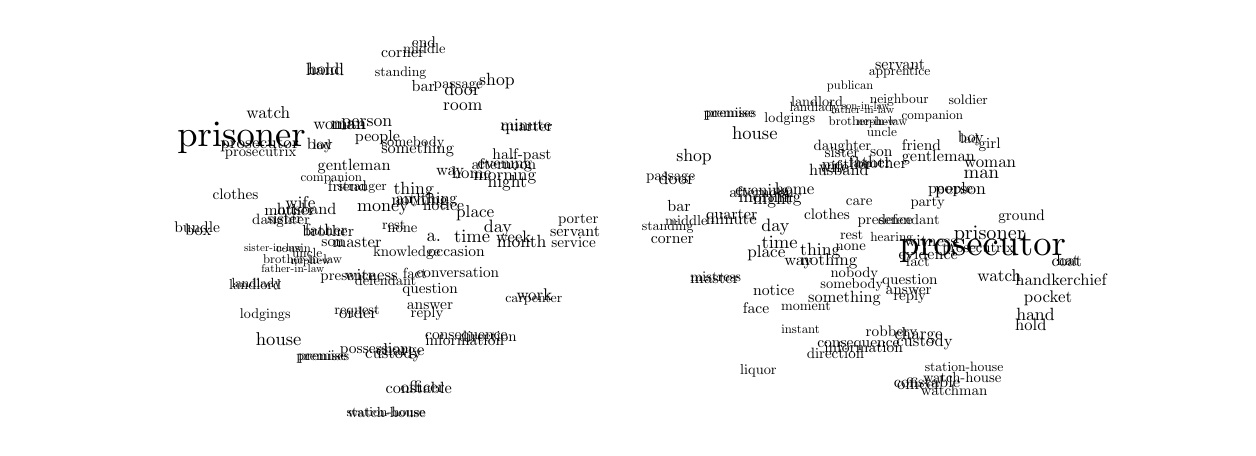
\begin{tikzpicture}[x=1pt,y=1pt]
\definecolor{fillColor}{RGB}{255,255,255}
\path[use as bounding box,fill=fillColor,fill opacity=0.00] (0,0) rectangle (433.62,144.54);
\begin{scope}
\path[clip] (  0.00,  0.00) rectangle (433.62,144.54);
\definecolor{drawColor}{RGB}{0,0,0}

\node[text=drawColor,anchor=base,inner sep=0pt, outer sep=0pt, scale=  1.32] at ( 77.29,101.53) {prisoner};

\node[text=drawColor,anchor=base,inner sep=0pt, outer sep=0pt, scale=  0.62] at ( 83.80,101.01) {prosecutor};

\node[text=drawColor,anchor=base,inner sep=0pt, outer sep=0pt, scale=  0.60] at (124.17, 53.15) {witness};

\node[text=drawColor,anchor=base,inner sep=0pt, outer sep=0pt, scale=  0.62] at ( 98.55, 79.09) {wife};

\node[text=drawColor,anchor=base,inner sep=0pt, outer sep=0pt, scale=  0.60] at (172.46, 93.75) {evening};

\node[text=drawColor,anchor=base,inner sep=0pt, outer sep=0pt, scale=  0.58] at (108.60, 69.06) {brother};

\node[text=drawColor,anchor=base,inner sep=0pt, outer sep=0pt, scale=  0.59] at (100.81, 76.96) {husband};

\node[text=drawColor,anchor=base,inner sep=0pt, outer sep=0pt, scale=  0.59] at (107.82, 69.62) {father};

\node[text=drawColor,anchor=base,inner sep=0pt, outer sep=0pt, scale=  0.63] at (172.44, 89.40) {morning};

\node[text=drawColor,anchor=base,inner sep=0pt, outer sep=0pt, scale=  0.68] at (115.94,107.85) {man};

\node[text=drawColor,anchor=base,inner sep=0pt, outer sep=0pt, scale=  0.53] at ( 84.21, 97.94) {prosecutrix};

\node[text=drawColor,anchor=base,inner sep=0pt, outer sep=0pt, scale=  0.60] at (132.16, 24.96) {custody};

\node[text=drawColor,anchor=base,inner sep=0pt, outer sep=0pt, scale=  0.56] at (172.10, 93.28) {afternoon};

\node[text=drawColor,anchor=base,inner sep=0pt, outer sep=0pt, scale=  0.59] at (105.55,100.66) {boy};

\node[text=drawColor,anchor=base,inner sep=0pt, outer sep=0pt, scale=  0.59] at (117.99, 92.94) {gentleman};

\node[text=drawColor,anchor=base,inner sep=0pt, outer sep=0pt, scale=  0.62] at (134.65, 26.11) {charge};

\node[text=drawColor,anchor=base,inner sep=0pt, outer sep=0pt, scale=  0.58] at (142.97,121.57) {bar};

\node[text=drawColor,anchor=base,inner sep=0pt, outer sep=0pt, scale=  0.58] at (197.79, 69.21) {servant};

\node[text=drawColor,anchor=base,inner sep=0pt, outer sep=0pt, scale=  0.67] at (160.61, 66.84) {time};

\node[text=drawColor,anchor=base,inner sep=0pt, outer sep=0pt, scale=  0.59] at (141.30, 12.45) {constable};

\node[text=drawColor,anchor=base,inner sep=0pt, outer sep=0pt, scale=  0.62] at (141.74, 80.16) {nothing};

\node[text=drawColor,anchor=base,inner sep=0pt, outer sep=0pt, scale=  0.55] at ( 92.94, 73.88) {sister};

\node[text=drawColor,anchor=base,inner sep=0pt, outer sep=0pt, scale=  0.60] at (142.72, 12.62) {officer};

\node[text=drawColor,anchor=base,inner sep=0pt, outer sep=0pt, scale=  0.61] at (112.68,107.87) {woman};

\node[text=drawColor,anchor=base,inner sep=0pt, outer sep=0pt, scale=  0.61] at (160.40, 90.03) {home};

\node[text=drawColor,anchor=base,inner sep=0pt, outer sep=0pt, scale=  0.64] at (169.59,123.57) {shop};

\node[text=drawColor,anchor=base,inner sep=0pt, outer sep=0pt, scale=  0.58] at ( 94.56, 76.75) {mother};

\node[text=drawColor,anchor=base,inner sep=0pt, outer sep=0pt, scale=  0.64] at (122.54,108.95) {person};

\node[text=drawColor,anchor=base,inner sep=0pt, outer sep=0pt, scale=  0.54] at (115.72, 53.30) {presence};

\node[text=drawColor,anchor=base,inner sep=0pt, outer sep=0pt, scale=  0.64] at (107.46,127.10) {hand};

\node[text=drawColor,anchor=base,inner sep=0pt, outer sep=0pt, scale=  0.63] at (173.28, 86.84) {night};

\node[text=drawColor,anchor=base,inner sep=0pt, outer sep=0pt, scale=  0.50] at (106.36,100.46) {lad};

\node[text=drawColor,anchor=base,inner sep=0pt, outer sep=0pt, scale=  0.52] at (129.32, 51.51) {defendant};

\node[text=drawColor,anchor=base,inner sep=0pt, outer sep=0pt, scale=  0.64] at (139.49, 84.26) {thing};

\node[text=drawColor,anchor=base,inner sep=0pt, outer sep=0pt, scale=  0.56] at (110.23, 65.59) {son};

\node[text=drawColor,anchor=base,inner sep=0pt, outer sep=0pt, scale=  0.67] at ( 90.69, 29.77) {house};

\node[text=drawColor,anchor=base,inner sep=0pt, outer sep=0pt, scale=  0.54] at ( 91.58, 73.45) {daughter};

\node[text=drawColor,anchor=base,inner sep=0pt, outer sep=0pt, scale=  0.65] at (169.92, 70.42) {day};

\node[text=drawColor,anchor=base,inner sep=0pt, outer sep=0pt, scale=  0.46] at ( 99.35, 59.20) {brother-in-law};

\node[text=drawColor,anchor=base,inner sep=0pt, outer sep=0pt, scale=  0.61] at (180.00,107.26) {minute};

\node[text=drawColor,anchor=base,inner sep=0pt, outer sep=0pt, scale=  0.60] at (152.65, 91.26) {way};

\node[text=drawColor,anchor=base,inner sep=0pt, outer sep=0pt, scale=  0.55] at (145.39, 48.55) {question};

\node[text=drawColor,anchor=base,inner sep=0pt, outer sep=0pt, scale=  0.53] at (135.42, 70.55) {none};

\node[text=drawColor,anchor=base,inner sep=0pt, outer sep=0pt, scale=  0.47] at (109.73, 89.06) {companion};

\node[text=drawColor,anchor=base,inner sep=0pt, outer sep=0pt, scale=  0.57] at (150.26, 78.31) {notice};

\node[text=drawColor,anchor=base,inner sep=0pt, outer sep=0pt, scale=  0.59] at (140.90, 99.09) {something};

\node[text=drawColor,anchor=base,inner sep=0pt, outer sep=0pt, scale=  0.60] at (119.03, 64.95) {master};

\node[text=drawColor,anchor=base,inner sep=0pt, outer sep=0pt, scale=  0.56] at (178.60, 96.85) {half-past};

\node[text=drawColor,anchor=base,inner sep=0pt, outer sep=0pt, scale=  0.63] at (157.25,114.64) {room};

\node[text=drawColor,anchor=base,inner sep=0pt, outer sep=0pt, scale=  0.56] at (158.52, 31.78) {consequence};

\node[text=drawColor,anchor=base,inner sep=0pt, outer sep=0pt, scale=  0.65] at (156.96,119.94) {door};

\node[text=drawColor,anchor=base,inner sep=0pt, outer sep=0pt, scale=  0.51] at ( 85.85, 39.28) {lodgings};

\node[text=drawColor,anchor=base,inner sep=0pt, outer sep=0pt, scale=  0.58] at (180.40,106.87) {quarter};

\node[text=drawColor,anchor=base,inner sep=0pt, outer sep=0pt, scale=  0.62] at (161.74, 75.91) {place};

\node[text=drawColor,anchor=base,inner sep=0pt, outer sep=0pt, scale=  0.56] at (115.56, 85.20) {friend};

\node[text=drawColor,anchor=base,inner sep=0pt, outer sep=0pt, scale=  0.56] at (157.93, 29.66) {information};

\node[text=drawColor,anchor=base,inner sep=0pt, outer sep=0pt, scale=  0.57] at (135.53,133.65) {corner};

\node[text=drawColor,anchor=base,inner sep=0pt, outer sep=0pt, scale=  0.48] at (101.00, 61.33) {uncle};

\node[text=drawColor,anchor=base,inner sep=0pt, outer sep=0pt, scale=  0.46] at ( 96.08, 63.41) {cousin};

\node[text=drawColor,anchor=base,inner sep=0pt, outer sep=0pt, scale=  0.52] at (139.21,101.63) {somebody};

\node[text=drawColor,anchor=base,inner sep=0pt, outer sep=0pt, scale=  0.60] at (175.60, 67.06) {week};

\node[text=drawColor,anchor=base,inner sep=0pt, outer sep=0pt, scale=  0.52] at (132.31, 71.68) {rest};

\node[text=drawColor,anchor=base,inner sep=0pt, outer sep=0pt, scale=  0.58] at (144.19, 80.96) {anything};

\node[text=drawColor,anchor=base,inner sep=0pt, outer sep=0pt, scale=  0.60] at (107.01,127.59) {hold};

\node[text=drawColor,anchor=base,inner sep=0pt, outer sep=0pt, scale=  0.67] at (146.76, 67.27) {a.};

\node[text=drawColor,anchor=base,inner sep=0pt, outer sep=0pt, scale=  0.65] at (128.36, 78.07) {money};

\node[text=drawColor,anchor=base,inner sep=0pt, outer sep=0pt, scale=  0.56] at ( 61.25, 70.44) {bundle};

\node[text=drawColor,anchor=base,inner sep=0pt, outer sep=0pt, scale=  0.50] at (134.76,126.78) {standing};

\node[text=drawColor,anchor=base,inner sep=0pt, outer sep=0pt, scale=  0.40] at ( 88.71, 63.62) {sister-in-law};

\node[text=drawColor,anchor=base,inner sep=0pt, outer sep=0pt, scale=  0.56] at (154.95, 62.01) {occasion};

\node[text=drawColor,anchor=base,inner sep=0pt, outer sep=0pt, scale=  0.61] at (183.09, 45.79) {work};

\node[text=drawColor,anchor=base,inner sep=0pt, outer sep=0pt, scale=  0.50] at (120.89, 85.87) {stranger};

\node[text=drawColor,anchor=base,inner sep=0pt, outer sep=0pt, scale=  0.49] at (129.47,  4.19) {station-house};

\node[text=drawColor,anchor=base,inner sep=0pt, outer sep=0pt, scale=  0.52] at (143.34,135.33) {middle};

\node[text=drawColor,anchor=base,inner sep=0pt, outer sep=0pt, scale=  0.55] at (197.24, 65.07) {service};

\node[text=drawColor,anchor=base,inner sep=0pt, outer sep=0pt, scale=  0.62] at ( 86.95,111.67) {watch};

\node[text=drawColor,anchor=base,inner sep=0pt, outer sep=0pt, scale=  0.60] at ( 61.60, 69.42) {box};

\node[text=drawColor,anchor=base,inner sep=0pt, outer sep=0pt, scale=  0.41] at ( 95.80, 55.99) {father-in-law};

\node[text=drawColor,anchor=base,inner sep=0pt, outer sep=0pt, scale=  0.54] at (198.93, 73.95) {porter};

\node[text=drawColor,anchor=base,inner sep=0pt, outer sep=0pt, scale=  0.56] at (145.39, 42.72) {answer};

\node[text=drawColor,anchor=base,inner sep=0pt, outer sep=0pt, scale=  0.54] at (155.61,122.65) {passage};

\node[text=drawColor,anchor=base,inner sep=0pt, outer sep=0pt, scale=  0.60] at (119.35, 39.39) {order};

\node[text=drawColor,anchor=base,inner sep=0pt, outer sep=0pt, scale=  0.44] at (102.29, 58.93) {nephew};

\node[text=drawColor,anchor=base,inner sep=0pt, outer sep=0pt, scale=  0.50] at (182.90, 45.32) {carpenter};

\node[text=drawColor,anchor=base,inner sep=0pt, outer sep=0pt, scale=  0.58] at (126.38,103.27) {people};

\node[text=drawColor,anchor=base,inner sep=0pt, outer sep=0pt, scale=  0.53] at (129.72,  3.53) {watch-house};

\node[text=drawColor,anchor=base,inner sep=0pt, outer sep=0pt, scale=  0.54] at (144.32, 39.79) {reply};

\node[text=drawColor,anchor=base,inner sep=0pt, outer sep=0pt, scale=  0.64] at (178.52, 65.09) {month};

\node[text=drawColor,anchor=base,inner sep=0pt, outer sep=0pt, scale=  0.55] at ( 75.11, 82.59) {clothes};

\node[text=drawColor,anchor=base,inner sep=0pt, outer sep=0pt, scale=  0.52] at ( 82.17, 49.82) {landlord};

\node[text=drawColor,anchor=base,inner sep=0pt, outer sep=0pt, scale=  0.51] at (106.64, 24.36) {premises};

\node[text=drawColor,anchor=base,inner sep=0pt, outer sep=0pt, scale=  0.53] at (139.93, 54.06) {fact};

\node[text=drawColor,anchor=base,inner sep=0pt, outer sep=0pt, scale=  0.54] at (136.94, 61.85) {knowledge};

\node[text=drawColor,anchor=base,inner sep=0pt, outer sep=0pt, scale=  0.56] at (143.21,137.25) {end};

\node[text=drawColor,anchor=base,inner sep=0pt, outer sep=0pt, scale=  0.56] at (125.25, 26.72) {possession};

\node[text=drawColor,anchor=base,inner sep=0pt, outer sep=0pt, scale=  0.52] at (119.02, 40.93) {request};

\node[text=drawColor,anchor=base,inner sep=0pt, outer sep=0pt, scale=  0.54] at (166.30, 31.01) {direction};

\node[text=drawColor,anchor=base,inner sep=0pt, outer sep=0pt, scale=  0.53] at (106.63, 24.29) {premise};

\node[text=drawColor,anchor=base,inner sep=0pt, outer sep=0pt, scale=  0.55] at (155.47, 54.28) {conversation};

\node[text=drawColor,anchor=base,inner sep=0pt, outer sep=0pt, scale=  0.48] at ( 82.70, 50.53) {landlady};
\end{scope}
\begin{scope}
\path[clip] (  0.00,  0.00) rectangle (433.62,144.54);
\definecolor{drawColor}{RGB}{0,0,0}

\node[text=drawColor,anchor=base,inner sep=0pt, outer sep=0pt, scale=  1.32] at (345.03, 62.19) {prosecutor};

\node[text=drawColor,anchor=base,inner sep=0pt, outer sep=0pt, scale=  0.53] at (343.42, 63.40) {prosecutrix};

\node[text=drawColor,anchor=base,inner sep=0pt, outer sep=0pt, scale=  0.73] at (347.46, 67.91) {prisoner};

\node[text=drawColor,anchor=base,inner sep=0pt, outer sep=0pt, scale=  0.60] at (326.30, 65.39) {witness};

\node[text=drawColor,anchor=base,inner sep=0pt, outer sep=0pt, scale=  0.59] at (324.94, 14.60) {constable};

\node[text=drawColor,anchor=base,inner sep=0pt, outer sep=0pt, scale=  0.59] at (293.14, 91.24) {husband};

\node[text=drawColor,anchor=base,inner sep=0pt, outer sep=0pt, scale=  0.62] at (291.40, 92.25) {wife};

\node[text=drawColor,anchor=base,inner sep=0pt, outer sep=0pt, scale=  0.58] at (308.33, 93.68) {brother};

\node[text=drawColor,anchor=base,inner sep=0pt, outer sep=0pt, scale=  0.59] at (329.07, 96.20) {gentleman};

\node[text=drawColor,anchor=base,inner sep=0pt, outer sep=0pt, scale=  0.59] at (304.30, 93.87) {father};

\node[text=drawColor,anchor=base,inner sep=0pt, outer sep=0pt, scale=  0.56] at (265.23, 83.23) {afternoon};

\node[text=drawColor,anchor=base,inner sep=0pt, outer sep=0pt, scale=  0.61] at (277.14, 84.37) {home};

\node[text=drawColor,anchor=base,inner sep=0pt, outer sep=0pt, scale=  0.63] at (268.28, 81.19) {morning};

\node[text=drawColor,anchor=base,inner sep=0pt, outer sep=0pt, scale=  0.60] at (265.54, 83.87) {evening};

\node[text=drawColor,anchor=base,inner sep=0pt, outer sep=0pt, scale=  0.59] at (340.84,102.95) {boy};

\node[text=drawColor,anchor=base,inner sep=0pt, outer sep=0pt, scale=  0.62] at (351.10, 52.75) {watch};

\node[text=drawColor,anchor=base,inner sep=0pt, outer sep=0pt, scale=  0.56] at (308.45, 98.03) {son};

\node[text=drawColor,anchor=base,inner sep=0pt, outer sep=0pt, scale=  0.54] at (294.42,100.24) {daughter};

\node[text=drawColor,anchor=base,inner sep=0pt, outer sep=0pt, scale=  0.58] at (315.27,129.26) {servant};

\node[text=drawColor,anchor=base,inner sep=0pt, outer sep=0pt, scale=  0.61] at (347.77, 94.07) {woman};

\node[text=drawColor,anchor=base,inner sep=0pt, outer sep=0pt, scale=  0.53] at (337.68, 16.15) {watch-house};

\node[text=drawColor,anchor=base,inner sep=0pt, outer sep=0pt, scale=  0.62] at (321.97, 31.74) {charge};

\node[text=drawColor,anchor=base,inner sep=0pt, outer sep=0pt, scale=  0.46] at (303.72,109.27) {brother-in-law};

\node[text=drawColor,anchor=base,inner sep=0pt, outer sep=0pt, scale=  0.52] at (285.23,115.92) {landlord};

\node[text=drawColor,anchor=base,inner sep=0pt, outer sep=0pt, scale=  0.55] at (359.17, 74.69) {ground};

\node[text=drawColor,anchor=base,inner sep=0pt, outer sep=0pt, scale=  0.50] at (340.37,102.75) {lad};

\node[text=drawColor,anchor=base,inner sep=0pt, outer sep=0pt, scale=  0.53] at (297.41, 64.08) {none};

\node[text=drawColor,anchor=base,inner sep=0pt, outer sep=0pt, scale=  0.67] at (262.75,104.00) {house};

\node[text=drawColor,anchor=base,inner sep=0pt, outer sep=0pt, scale=  0.60] at (278.48, 58.57) {way};

\node[text=drawColor,anchor=base,inner sep=0pt, outer sep=0pt, scale=  0.54] at (334.78, 11.63) {watchman};

\node[text=drawColor,anchor=base,inner sep=0pt, outer sep=0pt, scale=  0.63] at (269.12, 80.64) {night};

\node[text=drawColor,anchor=base,inner sep=0pt, outer sep=0pt, scale=  0.52] at (297.81, 50.45) {somebody};

\node[text=drawColor,anchor=base,inner sep=0pt, outer sep=0pt, scale=  0.60] at (324.08, 29.32) {custody};

\node[text=drawColor,anchor=base,inner sep=0pt, outer sep=0pt, scale=  0.48] at (284.34,114.30) {landlady};

\node[text=drawColor,anchor=base,inner sep=0pt, outer sep=0pt, scale=  0.56] at (302.09, 27.29) {information};

\node[text=drawColor,anchor=base,inner sep=0pt, outer sep=0pt, scale=  0.56] at (300.21, 28.81) {consequence};

\node[text=drawColor,anchor=base,inner sep=0pt, outer sep=0pt, scale=  0.60] at (248.26, 52.17) {master};

\node[text=drawColor,anchor=base,inner sep=0pt, outer sep=0pt, scale=  0.52] at (318.41, 73.57) {defendant};

\node[text=drawColor,anchor=base,inner sep=0pt, outer sep=0pt, scale=  0.49] at (338.37, 20.19) {station-house};

\node[text=drawColor,anchor=base,inner sep=0pt, outer sep=0pt, scale=  0.64] at (337.12, 84.36) {person};

\node[text=drawColor,anchor=base,inner sep=0pt, outer sep=0pt, scale=  0.56] at (322.96,100.18) {friend};

\node[text=drawColor,anchor=base,inner sep=0pt, outer sep=0pt, scale=  0.58] at (235.39, 78.08) {bar};

\node[text=drawColor,anchor=base,inner sep=0pt, outer sep=0pt, scale=  0.58] at (296.01, 93.23) {mother};

\node[text=drawColor,anchor=base,inner sep=0pt, outer sep=0pt, scale=  0.62] at (289.55, 58.55) {nothing};

\node[text=drawColor,anchor=base,inner sep=0pt, outer sep=0pt, scale=  0.52] at (297.76, 68.17) {rest};

\node[text=drawColor,anchor=base,inner sep=0pt, outer sep=0pt, scale=  0.68] at (344.61, 89.92) {man};

\node[text=drawColor,anchor=base,inner sep=0pt, outer sep=0pt, scale=  0.55] at (294.26, 97.58) {sister};

\node[text=drawColor,anchor=base,inner sep=0pt, outer sep=0pt, scale=  0.53] at (321.66, 58.41) {fact};

\node[text=drawColor,anchor=base,inner sep=0pt, outer sep=0pt, scale=  0.54] at (309.84, 73.29) {presence};

\node[text=drawColor,anchor=base,inner sep=0pt, outer sep=0pt, scale=  0.50] at (231.26, 71.10) {standing};

\node[text=drawColor,anchor=base,inner sep=0pt, outer sep=0pt, scale=  0.60] at (373.40, 51.36) {handkerchief};

\node[text=drawColor,anchor=base,inner sep=0pt, outer sep=0pt, scale=  0.51] at (275.38,110.11) {lodgings};

\node[text=drawColor,anchor=base,inner sep=0pt, outer sep=0pt, scale=  0.57] at (232.95, 66.72) {corner};

\node[text=drawColor,anchor=base,inner sep=0pt, outer sep=0pt, scale=  0.64] at (286.44, 62.16) {thing};

\node[text=drawColor,anchor=base,inner sep=0pt, outer sep=0pt, scale=  0.51] at (253.74,112.15) {premises};

\node[text=drawColor,anchor=base,inner sep=0pt, outer sep=0pt, scale=  0.58] at (325.39, 60.61) {evidence};

\node[text=drawColor,anchor=base,inner sep=0pt, outer sep=0pt, scale=  0.46] at (279.29, 34.21) {instant};

\node[text=drawColor,anchor=base,inner sep=0pt, outer sep=0pt, scale=  0.65] at (234.38, 88.02) {door};

\node[text=drawColor,anchor=base,inner sep=0pt, outer sep=0pt, scale=  0.58] at (333.47, 84.63) {people};

\node[text=drawColor,anchor=base,inner sep=0pt, outer sep=0pt, scale=  0.49] at (314.95,116.96) {neighbour};

\node[text=drawColor,anchor=base,inner sep=0pt, outer sep=0pt, scale=  0.64] at (364.17, 38.58) {hand};

\node[text=drawColor,anchor=base,inner sep=0pt, outer sep=0pt, scale=  0.52] at (264.05, 19.37) {liquor};

\node[text=drawColor,anchor=base,inner sep=0pt, outer sep=0pt, scale=  0.52] at (238.04, 73.00) {middle};

\node[text=drawColor,anchor=base,inner sep=0pt, outer sep=0pt, scale=  0.47] at (326.91,111.48) {companion};

\node[text=drawColor,anchor=base,inner sep=0pt, outer sep=0pt, scale=  0.50] at (339.86,116.62) {soldier};

\node[text=drawColor,anchor=base,inner sep=0pt, outer sep=0pt, scale=  0.44] at (306.74,109.28) {nephew};

\node[text=drawColor,anchor=base,inner sep=0pt, outer sep=0pt, scale=  0.55] at (347.61,100.95) {girl};

\node[text=drawColor,anchor=base,inner sep=0pt, outer sep=0pt, scale=  0.57] at (375.80, 58.50) {hat};

\node[text=drawColor,anchor=base,inner sep=0pt, outer sep=0pt, scale=  0.53] at (298.73, 54.12) {nobody};

\node[text=drawColor,anchor=base,inner sep=0pt, outer sep=0pt, scale=  0.67] at (271.70, 64.84) {time};

\node[text=drawColor,anchor=base,inner sep=0pt, outer sep=0pt, scale=  0.55] at (288.84, 75.12) {clothes};

\node[text=drawColor,anchor=base,inner sep=0pt, outer sep=0pt, scale=  0.61] at (368.70, 45.11) {pocket};

\node[text=drawColor,anchor=base,inner sep=0pt, outer sep=0pt, scale=  0.55] at (318.80, 51.66) {question};

\node[text=drawColor,anchor=base,inner sep=0pt, outer sep=0pt, scale=  0.57] at (269.57, 47.68) {notice};

\node[text=drawColor,anchor=base,inner sep=0pt, outer sep=0pt, scale=  0.61] at (254.22, 73.47) {minute};

\node[text=drawColor,anchor=base,inner sep=0pt, outer sep=0pt, scale=  0.60] at (322.02, 13.91) {officer};

\node[text=drawColor,anchor=base,inner sep=0pt, outer sep=0pt, scale=  0.65] at (270.21, 71.05) {day};

\node[text=drawColor,anchor=base,inner sep=0pt, outer sep=0pt, scale=  0.56] at (318.36, 47.99) {answer};

\node[text=drawColor,anchor=base,inner sep=0pt, outer sep=0pt, scale=  0.64] at (240.79, 96.35) {shop};

\node[text=drawColor,anchor=base,inner sep=0pt, outer sep=0pt, scale=  0.54] at (291.89, 24.94) {direction};

\node[text=drawColor,anchor=base,inner sep=0pt, outer sep=0pt, scale=  0.39] at (302.80,114.96) {son-in-law};

\node[text=drawColor,anchor=base,inner sep=0pt, outer sep=0pt, scale=  0.55] at (312.17, 32.85) {robbery};

\node[text=drawColor,anchor=base,inner sep=0pt, outer sep=0pt, scale=  0.54] at (232.38, 89.24) {passage};

\node[text=drawColor,anchor=base,inner sep=0pt, outer sep=0pt, scale=  0.60] at (362.49, 35.04) {hold};

\node[text=drawColor,anchor=base,inner sep=0pt, outer sep=0pt, scale=  0.45] at (297.21,122.35) {publican};

\node[text=drawColor,anchor=base,inner sep=0pt, outer sep=0pt, scale=  0.56] at (263.19, 41.12) {face};

\node[text=drawColor,anchor=base,inner sep=0pt, outer sep=0pt, scale=  0.54] at (318.72, 45.79) {reply};

\node[text=drawColor,anchor=base,inner sep=0pt, outer sep=0pt, scale=  0.53] at (325.20, 79.80) {party};

\node[text=drawColor,anchor=base,inner sep=0pt, outer sep=0pt, scale=  0.58] at (254.40, 75.21) {quarter};

\node[text=drawColor,anchor=base,inner sep=0pt, outer sep=0pt, scale=  0.48] at (308.69,105.17) {uncle};

\node[text=drawColor,anchor=base,inner sep=0pt, outer sep=0pt, scale=  0.52] at (248.65, 52.65) {mistress};

\node[text=drawColor,anchor=base,inner sep=0pt, outer sep=0pt, scale=  0.62] at (266.93, 61.40) {place};

\node[text=drawColor,anchor=base,inner sep=0pt, outer sep=0pt, scale=  0.41] at (301.73,113.38) {father-in-law};

\node[text=drawColor,anchor=base,inner sep=0pt, outer sep=0pt, scale=  0.54] at (300.51, 80.11) {care};

\node[text=drawColor,anchor=base,inner sep=0pt, outer sep=0pt, scale=  0.59] at (295.17, 45.16) {something};

\node[text=drawColor,anchor=base,inner sep=0pt, outer sep=0pt, scale=  0.48] at (312.21, 67.15) {hearing};

\node[text=drawColor,anchor=base,inner sep=0pt, outer sep=0pt, scale=  0.53] at (253.84,112.06) {premise};

\node[text=drawColor,anchor=base,inner sep=0pt, outer sep=0pt, scale=  0.60] at (375.51, 58.16) {coat};

\node[text=drawColor,anchor=base,inner sep=0pt, outer sep=0pt, scale=  0.51] at (281.22, 42.35) {moment};

\node[text=drawColor,anchor=base,inner sep=0pt, outer sep=0pt, scale=  0.49] at (315.07,127.43) {apprentice};
\end{scope}
\end{tikzpicture}

    \caption[Vector space neighbourhoods for \term{prisoner} and \term{prosecutor}]{
        Vector space neighbourhoods for \term{prisoner} and \term{prosecutor}.
    }
    \label{fig:glove_nns}
\end{figure}

Finally, the techniques discussed above with regards to the tracing of dimensions across the space is illustrated in \autoref{fig:glove_axes}.
This is the exercise that I'm proposing as the basic strategy for constructing $S \rightarrow \sigma \in \Sigma$ mappings, as it is (1) entirely endogenous and (2) not dependent on the absolute location of each term in the vector space.
More concretely, the image in the figure was constructed by tracing two axes across the vector space from the locations of terms that we can expect to be associated to sociologically relevant dimensions.
In this case I defined a first axis using the vector difference between $v_{man}$ and $v_{woman}$, i.e. a vector pointing to the location of \term{man} from the location of \term{woman} and a second axis using the vector difference between $v_{lord}$ and $v_{servant}$, i.e. a vector pointing to the location of \term{lord} from the location of \term{servant}, and then projecting all other vectors over these two in order to obtain the extent to which other terms fall along these two ``dimensions''.
Formally, the geometric interpretation of this exercise is that it is equivalent to projecting the high-dimensional vector space onto a two-dimensional plane spanned by the the two axes defined above.

\begin{figure}
    \centerfloat
    % Created by tikzDevice version 0.10.1 on 2017-12-08 11:30:11
% !TEX encoding = UTF-8 Unicode
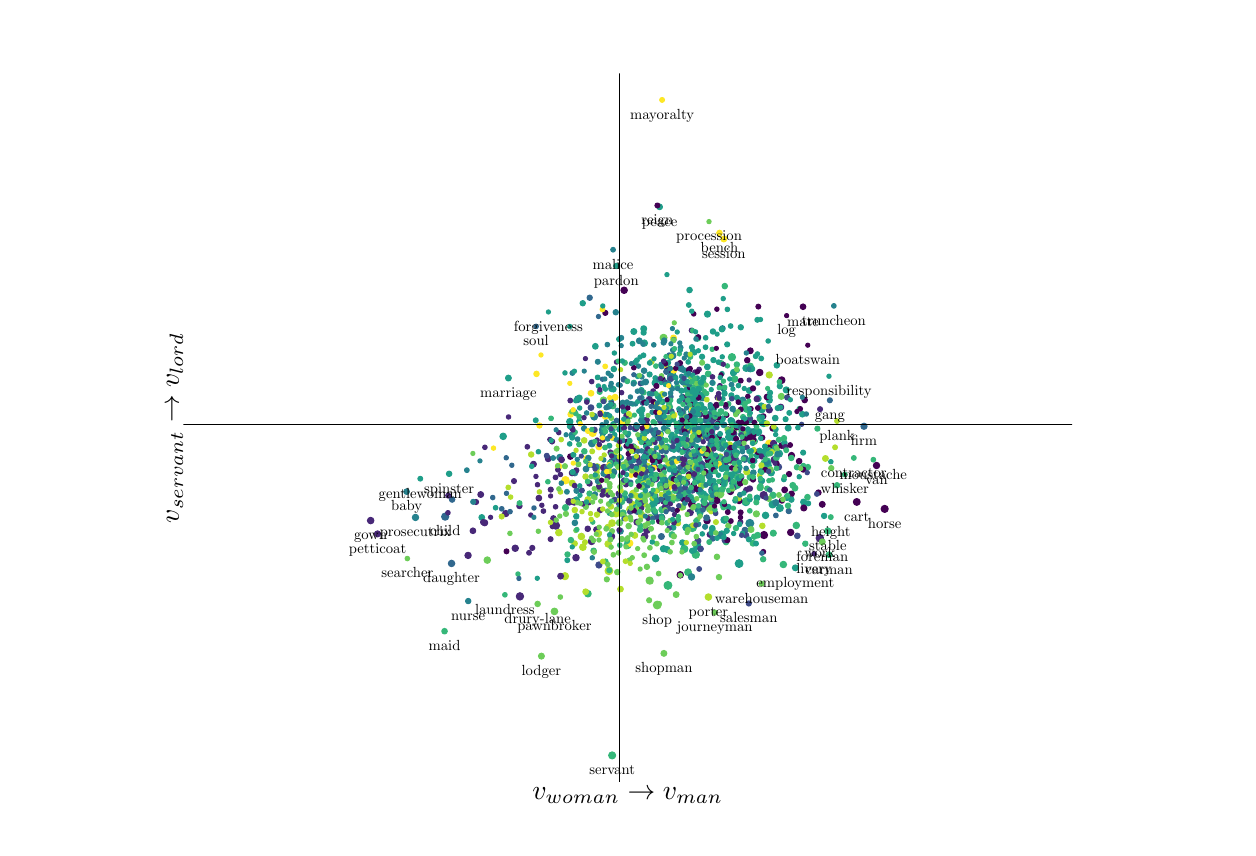
\begin{tikzpicture}[x=1pt,y=1pt]
\definecolor{fillColor}{RGB}{255,255,255}
\path[use as bounding box,fill=fillColor,fill opacity=0.00] (0,0) rectangle (433.62,289.08);
\begin{scope}
\path[clip] (  0.00,  0.00) rectangle (433.62,289.08);
\definecolor{drawColor}{RGB}{53,183,121}
\definecolor{fillColor}{RGB}{53,183,121}

\path[draw=drawColor,line width= 0.4pt,line join=round,line cap=round,fill=fillColor] (240.21,108.49) circle (  1.49);
\definecolor{drawColor}{RGB}{31,158,137}
\definecolor{fillColor}{RGB}{31,158,137}

\path[draw=drawColor,line width= 0.4pt,line join=round,line cap=round,fill=fillColor] (246.96,124.82) circle (  1.43);
\definecolor{drawColor}{RGB}{53,183,121}
\definecolor{fillColor}{RGB}{53,183,121}

\path[draw=drawColor,line width= 0.4pt,line join=round,line cap=round,fill=fillColor] (231.36, 87.55) circle (  1.41);
\definecolor{drawColor}{RGB}{38,130,142}
\definecolor{fillColor}{RGB}{38,130,142}

\path[draw=drawColor,line width= 0.4pt,line join=round,line cap=round,fill=fillColor] (260.95,109.98) circle (  1.41);
\definecolor{drawColor}{RGB}{109,205,89}
\definecolor{fillColor}{RGB}{109,205,89}

\path[draw=drawColor,line width= 0.4pt,line join=round,line cap=round,fill=fillColor] (227.48, 80.45) circle (  1.39);
\definecolor{drawColor}{RGB}{31,158,137}
\definecolor{fillColor}{RGB}{31,158,137}

\path[draw=drawColor,line width= 0.4pt,line join=round,line cap=round,fill=fillColor] (257.07, 95.43) circle (  1.39);

\path[draw=drawColor,line width= 0.4pt,line join=round,line cap=round,fill=fillColor] (259.53,117.74) circle (  1.39);

\path[draw=drawColor,line width= 0.4pt,line join=round,line cap=round,fill=fillColor] (250.81,105.86) circle (  1.39);
\definecolor{drawColor}{RGB}{180,222,44}
\definecolor{fillColor}{RGB}{180,222,44}

\path[draw=drawColor,line width= 0.4pt,line join=round,line cap=round,fill=fillColor] (210.03, 92.83) circle (  1.39);
\definecolor{drawColor}{RGB}{72,40,120}
\definecolor{fillColor}{RGB}{72,40,120}

\path[draw=drawColor,line width= 0.4pt,line join=round,line cap=round,fill=fillColor] (244.83,116.45) circle (  1.36);
\definecolor{drawColor}{RGB}{31,158,137}
\definecolor{fillColor}{RGB}{31,158,137}

\path[draw=drawColor,line width= 0.4pt,line join=round,line cap=round,fill=fillColor] (248.60,132.68) circle (  1.36);
\definecolor{drawColor}{RGB}{53,183,121}
\definecolor{fillColor}{RGB}{53,183,121}

\path[draw=drawColor,line width= 0.4pt,line join=round,line cap=round,fill=fillColor] (242.67,125.41) circle (  1.35);
\definecolor{drawColor}{RGB}{180,222,44}
\definecolor{fillColor}{RGB}{180,222,44}

\path[draw=drawColor,line width= 0.4pt,line join=round,line cap=round,fill=fillColor] (253.48,138.11) circle (  1.35);
\definecolor{drawColor}{RGB}{31,158,137}
\definecolor{fillColor}{RGB}{31,158,137}

\path[draw=drawColor,line width= 0.4pt,line join=round,line cap=round,fill=fillColor] (247.15,143.95) circle (  1.34);
\definecolor{drawColor}{RGB}{72,40,120}
\definecolor{fillColor}{RGB}{72,40,120}

\path[draw=drawColor,line width= 0.4pt,line join=round,line cap=round,fill=fillColor] (223.71,134.19) circle (  1.34);

\path[draw=drawColor,line width= 0.4pt,line join=round,line cap=round,fill=fillColor] (286.25,104.63) circle (  1.33);
\definecolor{drawColor}{RGB}{253,231,37}
\definecolor{fillColor}{RGB}{253,231,37}

\path[draw=drawColor,line width= 0.4pt,line join=round,line cap=round,fill=fillColor] (194.34,125.56) circle (  1.32);
\definecolor{drawColor}{RGB}{31,158,137}
\definecolor{fillColor}{RGB}{31,158,137}

\path[draw=drawColor,line width= 0.4pt,line join=round,line cap=round,fill=fillColor] (244.03,142.04) circle (  1.32);
\definecolor{drawColor}{RGB}{49,104,142}
\definecolor{fillColor}{RGB}{49,104,142}

\path[draw=drawColor,line width= 0.4pt,line join=round,line cap=round,fill=fillColor] (240.60,127.90) circle (  1.32);
\definecolor{drawColor}{RGB}{72,40,120}
\definecolor{fillColor}{RGB}{72,40,120}

\path[draw=drawColor,line width= 0.4pt,line join=round,line cap=round,fill=fillColor] (216.32,124.82) circle (  1.32);

\path[draw=drawColor,line width= 0.4pt,line join=round,line cap=round,fill=fillColor] (190.87,109.16) circle (  1.31);
\definecolor{drawColor}{RGB}{38,130,142}
\definecolor{fillColor}{RGB}{38,130,142}

\path[draw=drawColor,line width= 0.4pt,line join=round,line cap=round,fill=fillColor] (254.93,142.32) circle (  1.31);
\definecolor{drawColor}{RGB}{68,1,84}
\definecolor{fillColor}{RGB}{68,1,84}

\path[draw=drawColor,line width= 0.4pt,line join=round,line cap=round,fill=fillColor] (240.64,129.84) circle (  1.31);
\definecolor{drawColor}{RGB}{31,158,137}
\definecolor{fillColor}{RGB}{31,158,137}

\path[draw=drawColor,line width= 0.4pt,line join=round,line cap=round,fill=fillColor] (241.88,102.01) circle (  1.31);
\definecolor{drawColor}{RGB}{72,40,120}
\definecolor{fillColor}{RGB}{72,40,120}

\path[draw=drawColor,line width= 0.4pt,line join=round,line cap=round,fill=fillColor] (177.87, 83.58) circle (  1.31);
\definecolor{drawColor}{RGB}{53,183,121}
\definecolor{fillColor}{RGB}{53,183,121}

\path[draw=drawColor,line width= 0.4pt,line join=round,line cap=round,fill=fillColor] (241.43, 98.66) circle (  1.31);
\definecolor{drawColor}{RGB}{31,158,137}
\definecolor{fillColor}{RGB}{31,158,137}

\path[draw=drawColor,line width= 0.4pt,line join=round,line cap=round,fill=fillColor] (254.95,124.39) circle (  1.30);
\definecolor{drawColor}{RGB}{253,231,37}
\definecolor{fillColor}{RGB}{253,231,37}

\path[draw=drawColor,line width= 0.4pt,line join=round,line cap=round,fill=fillColor] (267.93,138.72) circle (  1.30);
\definecolor{drawColor}{RGB}{31,158,137}
\definecolor{fillColor}{RGB}{31,158,137}

\path[draw=drawColor,line width= 0.4pt,line join=round,line cap=round,fill=fillColor] (247.53,129.61) circle (  1.30);
\definecolor{drawColor}{RGB}{72,40,120}
\definecolor{fillColor}{RGB}{72,40,120}

\path[draw=drawColor,line width= 0.4pt,line join=round,line cap=round,fill=fillColor] (197.51,117.83) circle (  1.30);
\definecolor{drawColor}{RGB}{31,158,137}
\definecolor{fillColor}{RGB}{31,158,137}

\path[draw=drawColor,line width= 0.4pt,line join=round,line cap=round,fill=fillColor] (253.79,126.79) circle (  1.30);
\definecolor{drawColor}{RGB}{109,205,89}
\definecolor{fillColor}{RGB}{109,205,89}

\path[draw=drawColor,line width= 0.4pt,line join=round,line cap=round,fill=fillColor] (253.90,132.71) circle (  1.30);
\definecolor{drawColor}{RGB}{53,183,121}
\definecolor{fillColor}{RGB}{53,183,121}

\path[draw=drawColor,line width= 0.4pt,line join=round,line cap=round,fill=fillColor] (216.75,102.11) circle (  1.30);
\definecolor{drawColor}{RGB}{72,40,120}
\definecolor{fillColor}{RGB}{72,40,120}

\path[draw=drawColor,line width= 0.4pt,line join=round,line cap=round,fill=fillColor] (265.95,120.15) circle (  1.30);
\definecolor{drawColor}{RGB}{31,158,137}
\definecolor{fillColor}{RGB}{31,158,137}

\path[draw=drawColor,line width= 0.4pt,line join=round,line cap=round,fill=fillColor] (267.42,130.82) circle (  1.30);

\path[draw=drawColor,line width= 0.4pt,line join=round,line cap=round,fill=fillColor] (269.18,116.82) circle (  1.30);
\definecolor{drawColor}{RGB}{68,1,84}
\definecolor{fillColor}{RGB}{68,1,84}

\path[draw=drawColor,line width= 0.4pt,line join=round,line cap=round,fill=fillColor] (266.07,105.74) circle (  1.29);

\path[draw=drawColor,line width= 0.4pt,line join=round,line cap=round,fill=fillColor] (230.64,117.90) circle (  1.29);
\definecolor{drawColor}{RGB}{49,104,142}
\definecolor{fillColor}{RGB}{49,104,142}

\path[draw=drawColor,line width= 0.4pt,line join=round,line cap=round,fill=fillColor] (150.87,112.39) circle (  1.29);
\definecolor{drawColor}{RGB}{53,183,121}
\definecolor{fillColor}{RGB}{53,183,121}

\path[draw=drawColor,line width= 0.4pt,line join=round,line cap=round,fill=fillColor] (237.27,100.72) circle (  1.29);

\path[draw=drawColor,line width= 0.4pt,line join=round,line cap=round,fill=fillColor] (254.48,170.01) circle (  1.29);
\definecolor{drawColor}{RGB}{31,158,137}
\definecolor{fillColor}{RGB}{31,158,137}

\path[draw=drawColor,line width= 0.4pt,line join=round,line cap=round,fill=fillColor] (263.96,142.97) circle (  1.28);
\definecolor{drawColor}{RGB}{38,130,142}
\definecolor{fillColor}{RGB}{38,130,142}

\path[draw=drawColor,line width= 0.4pt,line join=round,line cap=round,fill=fillColor] (236.04,146.14) circle (  1.28);
\definecolor{drawColor}{RGB}{72,40,120}
\definecolor{fillColor}{RGB}{72,40,120}

\path[draw=drawColor,line width= 0.4pt,line join=round,line cap=round,fill=fillColor] (251.96,132.01) circle (  1.28);
\definecolor{drawColor}{RGB}{53,183,121}
\definecolor{fillColor}{RGB}{53,183,121}

\path[draw=drawColor,line width= 0.4pt,line join=round,line cap=round,fill=fillColor] (239.46,119.22) circle (  1.28);
\definecolor{drawColor}{RGB}{31,158,137}
\definecolor{fillColor}{RGB}{31,158,137}

\path[draw=drawColor,line width= 0.4pt,line join=round,line cap=round,fill=fillColor] (242.82,121.59) circle (  1.28);
\definecolor{drawColor}{RGB}{109,205,89}
\definecolor{fillColor}{RGB}{109,205,89}

\path[draw=drawColor,line width= 0.4pt,line join=round,line cap=round,fill=fillColor] (224.74, 89.29) circle (  1.28);
\definecolor{drawColor}{RGB}{49,104,142}
\definecolor{fillColor}{RGB}{49,104,142}

\path[draw=drawColor,line width= 0.4pt,line join=round,line cap=round,fill=fillColor] (259.10,133.30) circle (  1.27);

\path[draw=drawColor,line width= 0.4pt,line join=round,line cap=round,fill=fillColor] (235.69,121.08) circle (  1.27);
\definecolor{drawColor}{RGB}{31,158,137}
\definecolor{fillColor}{RGB}{31,158,137}

\path[draw=drawColor,line width= 0.4pt,line join=round,line cap=round,fill=fillColor] (271.49,135.14) circle (  1.27);
\definecolor{drawColor}{RGB}{180,222,44}
\definecolor{fillColor}{RGB}{180,222,44}

\path[draw=drawColor,line width= 0.4pt,line join=round,line cap=round,fill=fillColor] (194.16, 90.87) circle (  1.27);
\definecolor{drawColor}{RGB}{31,158,137}
\definecolor{fillColor}{RGB}{31,158,137}

\path[draw=drawColor,line width= 0.4pt,line join=round,line cap=round,fill=fillColor] (229.73,150.44) circle (  1.27);
\definecolor{drawColor}{RGB}{253,231,37}
\definecolor{fillColor}{RGB}{253,231,37}

\path[draw=drawColor,line width= 0.4pt,line join=round,line cap=round,fill=fillColor] (204.14,142.62) circle (  1.27);
\definecolor{drawColor}{RGB}{68,1,84}
\definecolor{fillColor}{RGB}{68,1,84}

\path[draw=drawColor,line width= 0.4pt,line join=round,line cap=round,fill=fillColor] (309.68,115.19) circle (  1.27);
\definecolor{drawColor}{RGB}{31,158,137}
\definecolor{fillColor}{RGB}{31,158,137}

\path[draw=drawColor,line width= 0.4pt,line join=round,line cap=round,fill=fillColor] (239.98,146.99) circle (  1.26);
\definecolor{drawColor}{RGB}{180,222,44}
\definecolor{fillColor}{RGB}{180,222,44}

\path[draw=drawColor,line width= 0.4pt,line join=round,line cap=round,fill=fillColor] (205.79,130.24) circle (  1.26);
\definecolor{drawColor}{RGB}{31,158,137}
\definecolor{fillColor}{RGB}{31,158,137}

\path[draw=drawColor,line width= 0.4pt,line join=round,line cap=round,fill=fillColor] (251.77,111.23) circle (  1.26);

\path[draw=drawColor,line width= 0.4pt,line join=round,line cap=round,fill=fillColor] (243.10,152.58) circle (  1.26);
\definecolor{drawColor}{RGB}{53,183,121}
\definecolor{fillColor}{RGB}{53,183,121}

\path[draw=drawColor,line width= 0.4pt,line join=round,line cap=round,fill=fillColor] (211.20, 26.11) circle (  1.26);
\definecolor{drawColor}{RGB}{109,205,89}
\definecolor{fillColor}{RGB}{109,205,89}

\path[draw=drawColor,line width= 0.4pt,line join=round,line cap=round,fill=fillColor] (229.77,177.04) circle (  1.25);
\definecolor{drawColor}{RGB}{53,183,121}
\definecolor{fillColor}{RGB}{53,183,121}

\path[draw=drawColor,line width= 0.4pt,line join=round,line cap=round,fill=fillColor] (226.09,118.81) circle (  1.25);
\definecolor{drawColor}{RGB}{109,205,89}
\definecolor{fillColor}{RGB}{109,205,89}

\path[draw=drawColor,line width= 0.4pt,line join=round,line cap=round,fill=fillColor] (237.92,160.32) circle (  1.25);
\definecolor{drawColor}{RGB}{68,1,84}
\definecolor{fillColor}{RGB}{68,1,84}

\path[draw=drawColor,line width= 0.4pt,line join=round,line cap=round,fill=fillColor] (237.19,118.91) circle (  1.25);

\path[draw=drawColor,line width= 0.4pt,line join=round,line cap=round,fill=fillColor] (228.96,112.00) circle (  1.24);
\definecolor{drawColor}{RGB}{31,158,137}
\definecolor{fillColor}{RGB}{31,158,137}

\path[draw=drawColor,line width= 0.4pt,line join=round,line cap=round,fill=fillColor] (271.80,115.47) circle (  1.24);
\definecolor{drawColor}{RGB}{72,40,120}
\definecolor{fillColor}{RGB}{72,40,120}

\path[draw=drawColor,line width= 0.4pt,line join=round,line cap=round,fill=fillColor] (223.50,145.44) circle (  1.23);
\definecolor{drawColor}{RGB}{253,231,37}
\definecolor{fillColor}{RGB}{253,231,37}

\path[draw=drawColor,line width= 0.4pt,line join=round,line cap=round,fill=fillColor] (231.44,122.96) circle (  1.23);
\definecolor{drawColor}{RGB}{72,40,120}
\definecolor{fillColor}{RGB}{72,40,120}

\path[draw=drawColor,line width= 0.4pt,line join=round,line cap=round,fill=fillColor] (269.85,132.92) circle (  1.23);
\definecolor{drawColor}{RGB}{53,183,121}
\definecolor{fillColor}{RGB}{53,183,121}

\path[draw=drawColor,line width= 0.4pt,line join=round,line cap=round,fill=fillColor] (239.83,138.99) circle (  1.23);
\definecolor{drawColor}{RGB}{68,1,84}
\definecolor{fillColor}{RGB}{68,1,84}

\path[draw=drawColor,line width= 0.4pt,line join=round,line cap=round,fill=fillColor] (299.59,117.70) circle (  1.22);
\definecolor{drawColor}{RGB}{53,183,121}
\definecolor{fillColor}{RGB}{53,183,121}

\path[draw=drawColor,line width= 0.4pt,line join=round,line cap=round,fill=fillColor] (259.66,117.97) circle (  1.22);
\definecolor{drawColor}{RGB}{109,205,89}
\definecolor{fillColor}{RGB}{109,205,89}

\path[draw=drawColor,line width= 0.4pt,line join=round,line cap=round,fill=fillColor] (229.49,127.03) circle (  1.22);
\definecolor{drawColor}{RGB}{31,158,137}
\definecolor{fillColor}{RGB}{31,158,137}

\path[draw=drawColor,line width= 0.4pt,line join=round,line cap=round,fill=fillColor] (262.41,142.98) circle (  1.22);
\definecolor{drawColor}{RGB}{53,183,121}
\definecolor{fillColor}{RGB}{53,183,121}

\path[draw=drawColor,line width= 0.4pt,line join=round,line cap=round,fill=fillColor] (244.16,136.58) circle (  1.22);
\definecolor{drawColor}{RGB}{31,158,137}
\definecolor{fillColor}{RGB}{31,158,137}

\path[draw=drawColor,line width= 0.4pt,line join=round,line cap=round,fill=fillColor] (238.82,157.84) circle (  1.22);
\definecolor{drawColor}{RGB}{38,130,142}
\definecolor{fillColor}{RGB}{38,130,142}

\path[draw=drawColor,line width= 0.4pt,line join=round,line cap=round,fill=fillColor] (218.85,133.07) circle (  1.22);
\definecolor{drawColor}{RGB}{53,183,121}
\definecolor{fillColor}{RGB}{53,183,121}

\path[draw=drawColor,line width= 0.4pt,line join=round,line cap=round,fill=fillColor] (231.82,152.03) circle (  1.22);
\definecolor{drawColor}{RGB}{38,130,142}
\definecolor{fillColor}{RGB}{38,130,142}

\path[draw=drawColor,line width= 0.4pt,line join=round,line cap=round,fill=fillColor] (203.89,138.83) circle (  1.22);
\definecolor{drawColor}{RGB}{180,222,44}
\definecolor{fillColor}{RGB}{180,222,44}

\path[draw=drawColor,line width= 0.4pt,line join=round,line cap=round,fill=fillColor] (232.49,124.88) circle (  1.22);
\definecolor{drawColor}{RGB}{38,130,142}
\definecolor{fillColor}{RGB}{38,130,142}

\path[draw=drawColor,line width= 0.4pt,line join=round,line cap=round,fill=fillColor] (240.06,134.46) circle (  1.22);
\definecolor{drawColor}{RGB}{31,158,137}
\definecolor{fillColor}{RGB}{31,158,137}

\path[draw=drawColor,line width= 0.4pt,line join=round,line cap=round,fill=fillColor] (268.62,128.30) circle (  1.21);
\definecolor{drawColor}{RGB}{38,130,142}
\definecolor{fillColor}{RGB}{38,130,142}

\path[draw=drawColor,line width= 0.4pt,line join=round,line cap=round,fill=fillColor] (204.71,148.50) circle (  1.21);
\definecolor{drawColor}{RGB}{68,1,84}
\definecolor{fillColor}{RGB}{68,1,84}

\path[draw=drawColor,line width= 0.4pt,line join=round,line cap=round,fill=fillColor] (239.98,116.78) circle (  1.21);
\definecolor{drawColor}{RGB}{31,158,137}
\definecolor{fillColor}{RGB}{31,158,137}

\path[draw=drawColor,line width= 0.4pt,line join=round,line cap=round,fill=fillColor] (226.92, 97.27) circle (  1.21);
\definecolor{drawColor}{RGB}{53,183,121}
\definecolor{fillColor}{RGB}{53,183,121}

\path[draw=drawColor,line width= 0.4pt,line join=round,line cap=round,fill=fillColor] (266.12,131.61) circle (  1.21);
\definecolor{drawColor}{RGB}{31,158,137}
\definecolor{fillColor}{RGB}{31,158,137}

\path[draw=drawColor,line width= 0.4pt,line join=round,line cap=round,fill=fillColor] (247.35,118.70) circle (  1.21);
\definecolor{drawColor}{RGB}{253,231,37}
\definecolor{fillColor}{RGB}{253,231,37}

\path[draw=drawColor,line width= 0.4pt,line join=round,line cap=round,fill=fillColor] (221.01,127.48) circle (  1.21);
\definecolor{drawColor}{RGB}{38,130,142}
\definecolor{fillColor}{RGB}{38,130,142}

\path[draw=drawColor,line width= 0.4pt,line join=round,line cap=round,fill=fillColor] (198.80,154.82) circle (  1.21);
\definecolor{drawColor}{RGB}{31,158,137}
\definecolor{fillColor}{RGB}{31,158,137}

\path[draw=drawColor,line width= 0.4pt,line join=round,line cap=round,fill=fillColor] (241.94,155.48) circle (  1.20);

\path[draw=drawColor,line width= 0.4pt,line join=round,line cap=round,fill=fillColor] (221.44,119.15) circle (  1.20);
\definecolor{drawColor}{RGB}{38,130,142}
\definecolor{fillColor}{RGB}{38,130,142}

\path[draw=drawColor,line width= 0.4pt,line join=round,line cap=round,fill=fillColor] (228.04,150.95) circle (  1.20);
\definecolor{drawColor}{RGB}{49,104,142}
\definecolor{fillColor}{RGB}{49,104,142}

\path[draw=drawColor,line width= 0.4pt,line join=round,line cap=round,fill=fillColor] (247.45,117.25) circle (  1.20);
\definecolor{drawColor}{RGB}{31,158,137}
\definecolor{fillColor}{RGB}{31,158,137}

\path[draw=drawColor,line width= 0.4pt,line join=round,line cap=round,fill=fillColor] (230.59,147.26) circle (  1.20);
\definecolor{drawColor}{RGB}{53,183,121}
\definecolor{fillColor}{RGB}{53,183,121}

\path[draw=drawColor,line width= 0.4pt,line join=round,line cap=round,fill=fillColor] (267.15,132.42) circle (  1.20);
\definecolor{drawColor}{RGB}{31,158,137}
\definecolor{fillColor}{RGB}{31,158,137}

\path[draw=drawColor,line width= 0.4pt,line join=round,line cap=round,fill=fillColor] (244.96,119.67) circle (  1.20);

\path[draw=drawColor,line width= 0.4pt,line join=round,line cap=round,fill=fillColor] (265.94,146.12) circle (  1.20);
\definecolor{drawColor}{RGB}{253,231,37}
\definecolor{fillColor}{RGB}{253,231,37}

\path[draw=drawColor,line width= 0.4pt,line join=round,line cap=round,fill=fillColor] (240.04,131.12) circle (  1.20);

\path[draw=drawColor,line width= 0.4pt,line join=round,line cap=round,fill=fillColor] (202.15,133.30) circle (  1.20);
\definecolor{drawColor}{RGB}{72,40,120}
\definecolor{fillColor}{RGB}{72,40,120}

\path[draw=drawColor,line width= 0.4pt,line join=round,line cap=round,fill=fillColor] (226.32,130.59) circle (  1.20);
\definecolor{drawColor}{RGB}{68,1,84}
\definecolor{fillColor}{RGB}{68,1,84}

\path[draw=drawColor,line width= 0.4pt,line join=round,line cap=round,fill=fillColor] (272.45,161.71) circle (  1.20);
\definecolor{drawColor}{RGB}{31,158,137}
\definecolor{fillColor}{RGB}{31,158,137}

\path[draw=drawColor,line width= 0.4pt,line join=round,line cap=round,fill=fillColor] (259.63,166.06) circle (  1.19);

\path[draw=drawColor,line width= 0.4pt,line join=round,line cap=round,fill=fillColor] (237.95,108.45) circle (  1.19);
\definecolor{drawColor}{RGB}{109,205,89}
\definecolor{fillColor}{RGB}{109,205,89}

\path[draw=drawColor,line width= 0.4pt,line join=round,line cap=round,fill=fillColor] (190.35, 78.14) circle (  1.19);
\definecolor{drawColor}{RGB}{72,40,120}
\definecolor{fillColor}{RGB}{72,40,120}

\path[draw=drawColor,line width= 0.4pt,line join=round,line cap=round,fill=fillColor] (195.67,117.76) circle (  1.19);
\definecolor{drawColor}{RGB}{180,222,44}
\definecolor{fillColor}{RGB}{180,222,44}

\path[draw=drawColor,line width= 0.4pt,line join=round,line cap=round,fill=fillColor] (233.29,119.18) circle (  1.19);
\definecolor{drawColor}{RGB}{53,183,121}
\definecolor{fillColor}{RGB}{53,183,121}

\path[draw=drawColor,line width= 0.4pt,line join=round,line cap=round,fill=fillColor] (238.62, 92.32) circle (  1.19);
\definecolor{drawColor}{RGB}{72,40,120}
\definecolor{fillColor}{RGB}{72,40,120}

\path[draw=drawColor,line width= 0.4pt,line join=round,line cap=round,fill=fillColor] (223.75,107.53) circle (  1.19);
\definecolor{drawColor}{RGB}{53,183,121}
\definecolor{fillColor}{RGB}{53,183,121}

\path[draw=drawColor,line width= 0.4pt,line join=round,line cap=round,fill=fillColor] (246.68,140.87) circle (  1.19);
\definecolor{drawColor}{RGB}{38,130,142}
\definecolor{fillColor}{RGB}{38,130,142}

\path[draw=drawColor,line width= 0.4pt,line join=round,line cap=round,fill=fillColor] (240.78,144.84) circle (  1.19);
\definecolor{drawColor}{RGB}{31,158,137}
\definecolor{fillColor}{RGB}{31,158,137}

\path[draw=drawColor,line width= 0.4pt,line join=round,line cap=round,fill=fillColor] (261.36,132.71) circle (  1.19);
\definecolor{drawColor}{RGB}{180,222,44}
\definecolor{fillColor}{RGB}{180,222,44}

\path[draw=drawColor,line width= 0.4pt,line join=round,line cap=round,fill=fillColor] (217.64,115.04) circle (  1.19);
\definecolor{drawColor}{RGB}{31,158,137}
\definecolor{fillColor}{RGB}{31,158,137}

\path[draw=drawColor,line width= 0.4pt,line join=round,line cap=round,fill=fillColor] (240.01,150.35) circle (  1.19);
\definecolor{drawColor}{RGB}{53,183,121}
\definecolor{fillColor}{RGB}{53,183,121}

\path[draw=drawColor,line width= 0.4pt,line join=round,line cap=round,fill=fillColor] (261.17,126.66) circle (  1.19);
\definecolor{drawColor}{RGB}{72,40,120}
\definecolor{fillColor}{RGB}{72,40,120}

\path[draw=drawColor,line width= 0.4pt,line join=round,line cap=round,fill=fillColor] (210.93,105.26) circle (  1.19);

\path[draw=drawColor,line width= 0.4pt,line join=round,line cap=round,fill=fillColor] (203.76,103.47) circle (  1.19);
\definecolor{drawColor}{RGB}{180,222,44}
\definecolor{fillColor}{RGB}{180,222,44}

\path[draw=drawColor,line width= 0.4pt,line join=round,line cap=round,fill=fillColor] (211.16,110.05) circle (  1.18);
\definecolor{drawColor}{RGB}{72,40,120}
\definecolor{fillColor}{RGB}{72,40,120}

\path[draw=drawColor,line width= 0.4pt,line join=round,line cap=round,fill=fillColor] (202.53,117.71) circle (  1.18);
\definecolor{drawColor}{RGB}{53,183,121}
\definecolor{fillColor}{RGB}{53,183,121}

\path[draw=drawColor,line width= 0.4pt,line join=round,line cap=round,fill=fillColor] (240.24,156.09) circle (  1.18);
\definecolor{drawColor}{RGB}{72,40,120}
\definecolor{fillColor}{RGB}{72,40,120}

\path[draw=drawColor,line width= 0.4pt,line join=round,line cap=round,fill=fillColor] (222.95,105.33) circle (  1.18);
\definecolor{drawColor}{RGB}{253,231,37}
\definecolor{fillColor}{RGB}{253,231,37}

\path[draw=drawColor,line width= 0.4pt,line join=round,line cap=round,fill=fillColor] (191.83,130.49) circle (  1.18);
\definecolor{drawColor}{RGB}{38,130,142}
\definecolor{fillColor}{RGB}{38,130,142}

\path[draw=drawColor,line width= 0.4pt,line join=round,line cap=round,fill=fillColor] (221.94,147.20) circle (  1.18);
\definecolor{drawColor}{RGB}{53,183,121}
\definecolor{fillColor}{RGB}{53,183,121}

\path[draw=drawColor,line width= 0.4pt,line join=round,line cap=round,fill=fillColor] (202.44, 84.54) circle (  1.18);
\definecolor{drawColor}{RGB}{180,222,44}
\definecolor{fillColor}{RGB}{180,222,44}

\path[draw=drawColor,line width= 0.4pt,line join=round,line cap=round,fill=fillColor] (200.62,101.35) circle (  1.18);
\definecolor{drawColor}{RGB}{72,40,120}
\definecolor{fillColor}{RGB}{72,40,120}

\path[draw=drawColor,line width= 0.4pt,line join=round,line cap=round,fill=fillColor] (208.23,130.08) circle (  1.17);

\path[draw=drawColor,line width= 0.4pt,line join=round,line cap=round,fill=fillColor] (222.36,127.30) circle (  1.17);
\definecolor{drawColor}{RGB}{180,222,44}
\definecolor{fillColor}{RGB}{180,222,44}

\path[draw=drawColor,line width= 0.4pt,line join=round,line cap=round,fill=fillColor] (200.07,105.22) circle (  1.17);
\definecolor{drawColor}{RGB}{38,130,142}
\definecolor{fillColor}{RGB}{38,130,142}

\path[draw=drawColor,line width= 0.4pt,line join=round,line cap=round,fill=fillColor] (211.72,141.07) circle (  1.17);
\definecolor{drawColor}{RGB}{31,158,137}
\definecolor{fillColor}{RGB}{31,158,137}

\path[draw=drawColor,line width= 0.4pt,line join=round,line cap=round,fill=fillColor] (265.07,152.32) circle (  1.17);
\definecolor{drawColor}{RGB}{49,104,142}
\definecolor{fillColor}{RGB}{49,104,142}

\path[draw=drawColor,line width= 0.4pt,line join=round,line cap=round,fill=fillColor] (246.83,115.37) circle (  1.17);
\definecolor{drawColor}{RGB}{72,40,120}
\definecolor{fillColor}{RGB}{72,40,120}

\path[draw=drawColor,line width= 0.4pt,line join=round,line cap=round,fill=fillColor] (239.36,113.90) circle (  1.17);

\path[draw=drawColor,line width= 0.4pt,line join=round,line cap=round,fill=fillColor] (198.13, 97.55) circle (  1.16);
\definecolor{drawColor}{RGB}{180,222,44}
\definecolor{fillColor}{RGB}{180,222,44}

\path[draw=drawColor,line width= 0.4pt,line join=round,line cap=round,fill=fillColor] (236.27,115.87) circle (  1.16);

\path[draw=drawColor,line width= 0.4pt,line join=round,line cap=round,fill=fillColor] (209.76,102.52) circle (  1.16);
\definecolor{drawColor}{RGB}{31,158,137}
\definecolor{fillColor}{RGB}{31,158,137}

\path[draw=drawColor,line width= 0.4pt,line join=round,line cap=round,fill=fillColor] (265.30,151.07) circle (  1.16);

\path[draw=drawColor,line width= 0.4pt,line join=round,line cap=round,fill=fillColor] (171.82,141.40) circle (  1.16);
\definecolor{drawColor}{RGB}{53,183,121}
\definecolor{fillColor}{RGB}{53,183,121}

\path[draw=drawColor,line width= 0.4pt,line join=round,line cap=round,fill=fillColor] (215.10,113.67) circle (  1.16);
\definecolor{drawColor}{RGB}{180,222,44}
\definecolor{fillColor}{RGB}{180,222,44}

\path[draw=drawColor,line width= 0.4pt,line join=round,line cap=round,fill=fillColor] (221.86,112.88) circle (  1.16);

\path[draw=drawColor,line width= 0.4pt,line join=round,line cap=round,fill=fillColor] (218.58,116.77) circle (  1.16);
\definecolor{drawColor}{RGB}{72,40,120}
\definecolor{fillColor}{RGB}{72,40,120}

\path[draw=drawColor,line width= 0.4pt,line join=round,line cap=round,fill=fillColor] (123.94,110.97) circle (  1.16);
\definecolor{drawColor}{RGB}{109,205,89}
\definecolor{fillColor}{RGB}{109,205,89}

\path[draw=drawColor,line width= 0.4pt,line join=round,line cap=round,fill=fillColor] (166.08, 96.68) circle (  1.16);
\definecolor{drawColor}{RGB}{31,158,137}
\definecolor{fillColor}{RGB}{31,158,137}

\path[draw=drawColor,line width= 0.4pt,line join=round,line cap=round,fill=fillColor] (264.69,148.19) circle (  1.16);
\definecolor{drawColor}{RGB}{53,183,121}
\definecolor{fillColor}{RGB}{53,183,121}

\path[draw=drawColor,line width= 0.4pt,line join=round,line cap=round,fill=fillColor] (256.86,138.37) circle (  1.16);
\definecolor{drawColor}{RGB}{253,231,37}
\definecolor{fillColor}{RGB}{253,231,37}

\path[draw=drawColor,line width= 0.4pt,line join=round,line cap=round,fill=fillColor] (240.30,150.97) circle (  1.16);
\definecolor{drawColor}{RGB}{109,205,89}
\definecolor{fillColor}{RGB}{109,205,89}

\path[draw=drawColor,line width= 0.4pt,line join=round,line cap=round,fill=fillColor] (208.08,154.48) circle (  1.16);
\definecolor{drawColor}{RGB}{68,1,84}
\definecolor{fillColor}{RGB}{68,1,84}

\path[draw=drawColor,line width= 0.4pt,line join=round,line cap=round,fill=fillColor] (235.80, 91.37) circle (  1.16);
\definecolor{drawColor}{RGB}{180,222,44}
\definecolor{fillColor}{RGB}{180,222,44}

\path[draw=drawColor,line width= 0.4pt,line join=round,line cap=round,fill=fillColor] (245.99, 83.34) circle (  1.16);

\path[draw=drawColor,line width= 0.4pt,line join=round,line cap=round,fill=fillColor] (191.93,106.62) circle (  1.16);
\definecolor{drawColor}{RGB}{253,231,37}
\definecolor{fillColor}{RGB}{253,231,37}

\path[draw=drawColor,line width= 0.4pt,line join=round,line cap=round,fill=fillColor] (208.82,148.65) circle (  1.15);
\definecolor{drawColor}{RGB}{68,1,84}
\definecolor{fillColor}{RGB}{68,1,84}

\path[draw=drawColor,line width= 0.4pt,line join=round,line cap=round,fill=fillColor] (264.53,164.48) circle (  1.15);
\definecolor{drawColor}{RGB}{72,40,120}
\definecolor{fillColor}{RGB}{72,40,120}

\path[draw=drawColor,line width= 0.4pt,line join=round,line cap=round,fill=fillColor] (257.65,126.66) circle (  1.15);
\definecolor{drawColor}{RGB}{31,158,137}
\definecolor{fillColor}{RGB}{31,158,137}

\path[draw=drawColor,line width= 0.4pt,line join=round,line cap=round,fill=fillColor] (232.96,163.87) circle (  1.15);
\definecolor{drawColor}{RGB}{38,130,142}
\definecolor{fillColor}{RGB}{38,130,142}

\path[draw=drawColor,line width= 0.4pt,line join=round,line cap=round,fill=fillColor] (254.53,146.51) circle (  1.15);
\definecolor{drawColor}{RGB}{180,222,44}
\definecolor{fillColor}{RGB}{180,222,44}

\path[draw=drawColor,line width= 0.4pt,line join=round,line cap=round,fill=fillColor] (230.08,123.06) circle (  1.15);
\definecolor{drawColor}{RGB}{53,183,121}
\definecolor{fillColor}{RGB}{53,183,121}

\path[draw=drawColor,line width= 0.4pt,line join=round,line cap=round,fill=fillColor] (273.06, 95.09) circle (  1.15);
\definecolor{drawColor}{RGB}{31,158,137}
\definecolor{fillColor}{RGB}{31,158,137}

\path[draw=drawColor,line width= 0.4pt,line join=round,line cap=round,fill=fillColor] (215.62,119.20) circle (  1.15);
\definecolor{drawColor}{RGB}{38,130,142}
\definecolor{fillColor}{RGB}{38,130,142}

\path[draw=drawColor,line width= 0.4pt,line join=round,line cap=round,fill=fillColor] (239.21,127.59) circle (  1.15);
\definecolor{drawColor}{RGB}{53,183,121}
\definecolor{fillColor}{RGB}{53,183,121}

\path[draw=drawColor,line width= 0.4pt,line join=round,line cap=round,fill=fillColor] (256.47,123.75) circle (  1.15);
\definecolor{drawColor}{RGB}{31,158,137}
\definecolor{fillColor}{RGB}{31,158,137}

\path[draw=drawColor,line width= 0.4pt,line join=round,line cap=round,fill=fillColor] (266.63,112.85) circle (  1.15);
\definecolor{drawColor}{RGB}{109,205,89}
\definecolor{fillColor}{RGB}{109,205,89}

\path[draw=drawColor,line width= 0.4pt,line join=round,line cap=round,fill=fillColor] (205.47,126.84) circle (  1.15);
\definecolor{drawColor}{RGB}{49,104,142}
\definecolor{fillColor}{RGB}{49,104,142}

\path[draw=drawColor,line width= 0.4pt,line join=round,line cap=round,fill=fillColor] (153.17, 95.48) circle (  1.15);
\definecolor{drawColor}{RGB}{31,158,137}
\definecolor{fillColor}{RGB}{31,158,137}

\path[draw=drawColor,line width= 0.4pt,line join=round,line cap=round,fill=fillColor] (250.48,131.13) circle (  1.15);
\definecolor{drawColor}{RGB}{68,1,84}
\definecolor{fillColor}{RGB}{68,1,84}

\path[draw=drawColor,line width= 0.4pt,line join=round,line cap=round,fill=fillColor] (215.53,194.19) circle (  1.15);
\definecolor{drawColor}{RGB}{53,183,121}
\definecolor{fillColor}{RGB}{53,183,121}

\path[draw=drawColor,line width= 0.4pt,line join=round,line cap=round,fill=fillColor] (251.92,138.23) circle (  1.15);

\path[draw=drawColor,line width= 0.4pt,line join=round,line cap=round,fill=fillColor] (277.74,109.21) circle (  1.15);
\definecolor{drawColor}{RGB}{68,1,84}
\definecolor{fillColor}{RGB}{68,1,84}

\path[draw=drawColor,line width= 0.4pt,line join=round,line cap=round,fill=fillColor] (251.10,124.91) circle (  1.15);
\definecolor{drawColor}{RGB}{31,158,137}
\definecolor{fillColor}{RGB}{31,158,137}

\path[draw=drawColor,line width= 0.4pt,line join=round,line cap=round,fill=fillColor] (250.51,147.19) circle (  1.14);
\definecolor{drawColor}{RGB}{38,130,142}
\definecolor{fillColor}{RGB}{38,130,142}

\path[draw=drawColor,line width= 0.4pt,line join=round,line cap=round,fill=fillColor] (233.11,170.52) circle (  1.14);
\definecolor{drawColor}{RGB}{31,158,137}
\definecolor{fillColor}{RGB}{31,158,137}

\path[draw=drawColor,line width= 0.4pt,line join=round,line cap=round,fill=fillColor] (265.09,128.75) circle (  1.14);

\path[draw=drawColor,line width= 0.4pt,line join=round,line cap=round,fill=fillColor] (195.89,146.72) circle (  1.14);
\definecolor{drawColor}{RGB}{53,183,121}
\definecolor{fillColor}{RGB}{53,183,121}

\path[draw=drawColor,line width= 0.4pt,line join=round,line cap=round,fill=fillColor] (255.50,162.10) circle (  1.14);
\definecolor{drawColor}{RGB}{31,158,137}
\definecolor{fillColor}{RGB}{31,158,137}

\path[draw=drawColor,line width= 0.4pt,line join=round,line cap=round,fill=fillColor] (239.86,148.59) circle (  1.14);
\definecolor{drawColor}{RGB}{38,130,142}
\definecolor{fillColor}{RGB}{38,130,142}

\path[draw=drawColor,line width= 0.4pt,line join=round,line cap=round,fill=fillColor] (231.32,165.47) circle (  1.14);
\definecolor{drawColor}{RGB}{31,158,137}
\definecolor{fillColor}{RGB}{31,158,137}

\path[draw=drawColor,line width= 0.4pt,line join=round,line cap=round,fill=fillColor] (238.92,143.68) circle (  1.14);
\definecolor{drawColor}{RGB}{38,130,142}
\definecolor{fillColor}{RGB}{38,130,142}

\path[draw=drawColor,line width= 0.4pt,line join=round,line cap=round,fill=fillColor] (207.84,142.82) circle (  1.14);
\definecolor{drawColor}{RGB}{109,205,89}
\definecolor{fillColor}{RGB}{109,205,89}

\path[draw=drawColor,line width= 0.4pt,line join=round,line cap=round,fill=fillColor] (264.69,122.91) circle (  1.14);
\definecolor{drawColor}{RGB}{68,1,84}
\definecolor{fillColor}{RGB}{68,1,84}

\path[draw=drawColor,line width= 0.4pt,line join=round,line cap=round,fill=fillColor] (241.91,134.70) circle (  1.14);
\definecolor{drawColor}{RGB}{53,183,121}
\definecolor{fillColor}{RGB}{53,183,121}

\path[draw=drawColor,line width= 0.4pt,line join=round,line cap=round,fill=fillColor] (250.53,137.19) circle (  1.14);
\definecolor{drawColor}{RGB}{38,130,142}
\definecolor{fillColor}{RGB}{38,130,142}

\path[draw=drawColor,line width= 0.4pt,line join=round,line cap=round,fill=fillColor] (240.24,129.88) circle (  1.14);
\definecolor{drawColor}{RGB}{53,183,121}
\definecolor{fillColor}{RGB}{53,183,121}

\path[draw=drawColor,line width= 0.4pt,line join=round,line cap=round,fill=fillColor] (289.12,107.19) circle (  1.14);

\path[draw=drawColor,line width= 0.4pt,line join=round,line cap=round,fill=fillColor] (224.53,129.25) circle (  1.14);
\definecolor{drawColor}{RGB}{62,74,137}
\definecolor{fillColor}{RGB}{62,74,137}

\path[draw=drawColor,line width= 0.4pt,line join=round,line cap=round,fill=fillColor] (235.33,119.29) circle (  1.14);
\definecolor{drawColor}{RGB}{38,130,142}
\definecolor{fillColor}{RGB}{38,130,142}

\path[draw=drawColor,line width= 0.4pt,line join=round,line cap=round,fill=fillColor] (239.87, 90.62) circle (  1.14);
\definecolor{drawColor}{RGB}{180,222,44}
\definecolor{fillColor}{RGB}{180,222,44}

\path[draw=drawColor,line width= 0.4pt,line join=round,line cap=round,fill=fillColor] (212.65,113.41) circle (  1.14);
\definecolor{drawColor}{RGB}{72,40,120}
\definecolor{fillColor}{RGB}{72,40,120}

\path[draw=drawColor,line width= 0.4pt,line join=round,line cap=round,fill=fillColor] (176.18,100.96) circle (  1.14);
\definecolor{drawColor}{RGB}{31,158,137}
\definecolor{fillColor}{RGB}{31,158,137}

\path[draw=drawColor,line width= 0.4pt,line join=round,line cap=round,fill=fillColor] (243.11,136.41) circle (  1.14);

\path[draw=drawColor,line width= 0.4pt,line join=round,line cap=round,fill=fillColor] (222.27,119.98) circle (  1.14);
\definecolor{drawColor}{RGB}{68,1,84}
\definecolor{fillColor}{RGB}{68,1,84}

\path[draw=drawColor,line width= 0.4pt,line join=round,line cap=round,fill=fillColor] (221.83,118.82) circle (  1.14);
\definecolor{drawColor}{RGB}{62,74,137}
\definecolor{fillColor}{RGB}{62,74,137}

\path[draw=drawColor,line width= 0.4pt,line join=round,line cap=round,fill=fillColor] (255.66,133.20) circle (  1.13);
\definecolor{drawColor}{RGB}{68,1,84}
\definecolor{fillColor}{RGB}{68,1,84}

\path[draw=drawColor,line width= 0.4pt,line join=round,line cap=round,fill=fillColor] (248.11,137.58) circle (  1.13);

\path[draw=drawColor,line width= 0.4pt,line join=round,line cap=round,fill=fillColor] (245.50,110.93) circle (  1.13);
\definecolor{drawColor}{RGB}{109,205,89}
\definecolor{fillColor}{RGB}{109,205,89}

\path[draw=drawColor,line width= 0.4pt,line join=round,line cap=round,fill=fillColor] (206.66,122.45) circle (  1.13);
\definecolor{drawColor}{RGB}{180,222,44}
\definecolor{fillColor}{RGB}{180,222,44}

\path[draw=drawColor,line width= 0.4pt,line join=round,line cap=round,fill=fillColor] (222.59,118.49) circle (  1.13);
\definecolor{drawColor}{RGB}{72,40,120}
\definecolor{fillColor}{RGB}{72,40,120}

\path[draw=drawColor,line width= 0.4pt,line join=round,line cap=round,fill=fillColor] (172.73,113.49) circle (  1.13);
\definecolor{drawColor}{RGB}{31,158,137}
\definecolor{fillColor}{RGB}{31,158,137}

\path[draw=drawColor,line width= 0.4pt,line join=round,line cap=round,fill=fillColor] (243.30,124.55) circle (  1.13);
\definecolor{drawColor}{RGB}{68,1,84}
\definecolor{fillColor}{RGB}{68,1,84}

\path[draw=drawColor,line width= 0.4pt,line join=round,line cap=round,fill=fillColor] (253.95,121.49) circle (  1.13);
\definecolor{drawColor}{RGB}{38,130,142}
\definecolor{fillColor}{RGB}{38,130,142}

\path[draw=drawColor,line width= 0.4pt,line join=round,line cap=round,fill=fillColor] (140.14,112.10) circle (  1.13);
\definecolor{drawColor}{RGB}{31,158,137}
\definecolor{fillColor}{RGB}{31,158,137}

\path[draw=drawColor,line width= 0.4pt,line join=round,line cap=round,fill=fillColor] (242.07,133.81) circle (  1.13);
\definecolor{drawColor}{RGB}{38,130,142}
\definecolor{fillColor}{RGB}{38,130,142}

\path[draw=drawColor,line width= 0.4pt,line join=round,line cap=round,fill=fillColor] (236.04,166.00) circle (  1.13);
\definecolor{drawColor}{RGB}{68,1,84}
\definecolor{fillColor}{RGB}{68,1,84}

\path[draw=drawColor,line width= 0.4pt,line join=round,line cap=round,fill=fillColor] (275.71,106.69) circle (  1.13);
\definecolor{drawColor}{RGB}{31,158,137}
\definecolor{fillColor}{RGB}{31,158,137}

\path[draw=drawColor,line width= 0.4pt,line join=round,line cap=round,fill=fillColor] (222.84,175.10) circle (  1.13);

\path[draw=drawColor,line width= 0.4pt,line join=round,line cap=round,fill=fillColor] (229.77,100.78) circle (  1.13);
\definecolor{drawColor}{RGB}{68,1,84}
\definecolor{fillColor}{RGB}{68,1,84}

\path[draw=drawColor,line width= 0.4pt,line join=round,line cap=round,fill=fillColor] (306.73,130.87) circle (  1.13);
\definecolor{drawColor}{RGB}{72,40,120}
\definecolor{fillColor}{RGB}{72,40,120}

\path[draw=drawColor,line width= 0.4pt,line join=round,line cap=round,fill=fillColor] (159.14, 98.38) circle (  1.13);
\definecolor{drawColor}{RGB}{31,158,137}
\definecolor{fillColor}{RGB}{31,158,137}

\path[draw=drawColor,line width= 0.4pt,line join=round,line cap=round,fill=fillColor] (263.92,155.08) circle (  1.13);
\definecolor{drawColor}{RGB}{53,183,121}
\definecolor{fillColor}{RGB}{53,183,121}

\path[draw=drawColor,line width= 0.4pt,line join=round,line cap=round,fill=fillColor] (233.81,141.16) circle (  1.13);

\path[draw=drawColor,line width= 0.4pt,line join=round,line cap=round,fill=fillColor] (243.98,160.73) circle (  1.12);
\definecolor{drawColor}{RGB}{49,104,142}
\definecolor{fillColor}{RGB}{49,104,142}

\path[draw=drawColor,line width= 0.4pt,line join=round,line cap=round,fill=fillColor] (245.21,134.32) circle (  1.12);
\definecolor{drawColor}{RGB}{72,40,120}
\definecolor{fillColor}{RGB}{72,40,120}

\path[draw=drawColor,line width= 0.4pt,line join=round,line cap=round,fill=fillColor] (269.54,138.83) circle (  1.12);

\path[draw=drawColor,line width= 0.4pt,line join=round,line cap=round,fill=fillColor] (241.96,157.83) circle (  1.12);
\definecolor{drawColor}{RGB}{53,183,121}
\definecolor{fillColor}{RGB}{53,183,121}

\path[draw=drawColor,line width= 0.4pt,line join=round,line cap=round,fill=fillColor] (229.19,114.90) circle (  1.12);

\path[draw=drawColor,line width= 0.4pt,line join=round,line cap=round,fill=fillColor] (236.69,150.12) circle (  1.12);

\path[draw=drawColor,line width= 0.4pt,line join=round,line cap=round,fill=fillColor] (243.13,158.89) circle (  1.12);

\path[draw=drawColor,line width= 0.4pt,line join=round,line cap=round,fill=fillColor] (211.41,152.46) circle (  1.12);
\definecolor{drawColor}{RGB}{68,1,84}
\definecolor{fillColor}{RGB}{68,1,84}

\path[draw=drawColor,line width= 0.4pt,line join=round,line cap=round,fill=fillColor] (226.63,142.51) circle (  1.12);
\definecolor{drawColor}{RGB}{109,205,89}
\definecolor{fillColor}{RGB}{109,205,89}

\path[draw=drawColor,line width= 0.4pt,line join=round,line cap=round,fill=fillColor] (213.85,110.20) circle (  1.12);
\definecolor{drawColor}{RGB}{49,104,142}
\definecolor{fillColor}{RGB}{49,104,142}

\path[draw=drawColor,line width= 0.4pt,line join=round,line cap=round,fill=fillColor] (232.28,162.29) circle (  1.12);
\definecolor{drawColor}{RGB}{62,74,137}
\definecolor{fillColor}{RGB}{62,74,137}

\path[draw=drawColor,line width= 0.4pt,line join=round,line cap=round,fill=fillColor] (255.09,142.36) circle (  1.12);
\definecolor{drawColor}{RGB}{31,158,137}
\definecolor{fillColor}{RGB}{31,158,137}

\path[draw=drawColor,line width= 0.4pt,line join=round,line cap=round,fill=fillColor] (238.23,158.15) circle (  1.11);
\definecolor{drawColor}{RGB}{49,104,142}
\definecolor{fillColor}{RGB}{49,104,142}

\path[draw=drawColor,line width= 0.4pt,line join=round,line cap=round,fill=fillColor] (246.91,149.63) circle (  1.11);

\path[draw=drawColor,line width= 0.4pt,line join=round,line cap=round,fill=fillColor] (302.20,145.04) circle (  1.11);
\definecolor{drawColor}{RGB}{31,158,137}
\definecolor{fillColor}{RGB}{31,158,137}

\path[draw=drawColor,line width= 0.4pt,line join=round,line cap=round,fill=fillColor] (240.60,133.86) circle (  1.11);

\path[draw=drawColor,line width= 0.4pt,line join=round,line cap=round,fill=fillColor] (270.31,137.40) circle (  1.11);

\path[draw=drawColor,line width= 0.4pt,line join=round,line cap=round,fill=fillColor] (228.43,140.80) circle (  1.11);

\path[draw=drawColor,line width= 0.4pt,line join=round,line cap=round,fill=fillColor] (247.98,139.54) circle (  1.11);
\definecolor{drawColor}{RGB}{53,183,121}
\definecolor{fillColor}{RGB}{53,183,121}

\path[draw=drawColor,line width= 0.4pt,line join=round,line cap=round,fill=fillColor] (227.49,134.43) circle (  1.11);
\definecolor{drawColor}{RGB}{31,158,137}
\definecolor{fillColor}{RGB}{31,158,137}

\path[draw=drawColor,line width= 0.4pt,line join=round,line cap=round,fill=fillColor] (247.99,151.70) circle (  1.11);
\definecolor{drawColor}{RGB}{253,231,37}
\definecolor{fillColor}{RGB}{253,231,37}

\path[draw=drawColor,line width= 0.4pt,line join=round,line cap=round,fill=fillColor] (217.57,102.79) circle (  1.11);
\definecolor{drawColor}{RGB}{180,222,44}
\definecolor{fillColor}{RGB}{180,222,44}

\path[draw=drawColor,line width= 0.4pt,line join=round,line cap=round,fill=fillColor] (222.17,125.31) circle (  1.11);
\definecolor{drawColor}{RGB}{31,158,137}
\definecolor{fillColor}{RGB}{31,158,137}

\path[draw=drawColor,line width= 0.4pt,line join=round,line cap=round,fill=fillColor] (212.28,132.62) circle (  1.11);
\definecolor{drawColor}{RGB}{72,40,120}
\definecolor{fillColor}{RGB}{72,40,120}

\path[draw=drawColor,line width= 0.4pt,line join=round,line cap=round,fill=fillColor] (248.15,123.33) circle (  1.11);
\definecolor{drawColor}{RGB}{31,158,137}
\definecolor{fillColor}{RGB}{31,158,137}

\path[draw=drawColor,line width= 0.4pt,line join=round,line cap=round,fill=fillColor] (230.80,121.68) circle (  1.11);
\definecolor{drawColor}{RGB}{53,183,121}
\definecolor{fillColor}{RGB}{53,183,121}

\path[draw=drawColor,line width= 0.4pt,line join=round,line cap=round,fill=fillColor] (239.14,119.23) circle (  1.11);

\path[draw=drawColor,line width= 0.4pt,line join=round,line cap=round,fill=fillColor] (242.05,176.86) circle (  1.11);
\definecolor{drawColor}{RGB}{38,130,142}
\definecolor{fillColor}{RGB}{38,130,142}

\path[draw=drawColor,line width= 0.4pt,line join=round,line cap=round,fill=fillColor] (232.32,163.18) circle (  1.11);
\definecolor{drawColor}{RGB}{31,158,137}
\definecolor{fillColor}{RGB}{31,158,137}

\path[draw=drawColor,line width= 0.4pt,line join=round,line cap=round,fill=fillColor] (254.15,135.56) circle (  1.11);
\definecolor{drawColor}{RGB}{72,40,120}
\definecolor{fillColor}{RGB}{72,40,120}

\path[draw=drawColor,line width= 0.4pt,line join=round,line cap=round,fill=fillColor] (248.85,131.70) circle (  1.11);
\definecolor{drawColor}{RGB}{62,74,137}
\definecolor{fillColor}{RGB}{62,74,137}

\path[draw=drawColor,line width= 0.4pt,line join=round,line cap=round,fill=fillColor] (206.42, 94.92) circle (  1.10);
\definecolor{drawColor}{RGB}{53,183,121}
\definecolor{fillColor}{RGB}{53,183,121}

\path[draw=drawColor,line width= 0.4pt,line join=round,line cap=round,fill=fillColor] (237.34,120.68) circle (  1.10);
\definecolor{drawColor}{RGB}{180,222,44}
\definecolor{fillColor}{RGB}{180,222,44}

\path[draw=drawColor,line width= 0.4pt,line join=round,line cap=round,fill=fillColor] (259.85,128.59) circle (  1.10);
\definecolor{drawColor}{RGB}{72,40,120}
\definecolor{fillColor}{RGB}{72,40,120}

\path[draw=drawColor,line width= 0.4pt,line join=round,line cap=round,fill=fillColor] (267.98,150.97) circle (  1.10);
\definecolor{drawColor}{RGB}{253,231,37}
\definecolor{fillColor}{RGB}{253,231,37}

\path[draw=drawColor,line width= 0.4pt,line join=round,line cap=round,fill=fillColor] (249.61,131.35) circle (  1.10);
\definecolor{drawColor}{RGB}{38,130,142}
\definecolor{fillColor}{RGB}{38,130,142}

\path[draw=drawColor,line width= 0.4pt,line join=round,line cap=round,fill=fillColor] (250.15,105.68) circle (  1.10);
\definecolor{drawColor}{RGB}{180,222,44}
\definecolor{fillColor}{RGB}{180,222,44}

\path[draw=drawColor,line width= 0.4pt,line join=round,line cap=round,fill=fillColor] (267.96,163.59) circle (  1.10);
\definecolor{drawColor}{RGB}{31,158,137}
\definecolor{fillColor}{RGB}{31,158,137}

\path[draw=drawColor,line width= 0.4pt,line join=round,line cap=round,fill=fillColor] (198.30,118.42) circle (  1.10);
\definecolor{drawColor}{RGB}{38,130,142}
\definecolor{fillColor}{RGB}{38,130,142}

\path[draw=drawColor,line width= 0.4pt,line join=round,line cap=round,fill=fillColor] (192.29,133.80) circle (  1.10);
\definecolor{drawColor}{RGB}{72,40,120}
\definecolor{fillColor}{RGB}{72,40,120}

\path[draw=drawColor,line width= 0.4pt,line join=round,line cap=round,fill=fillColor] (229.85,118.02) circle (  1.10);
\definecolor{drawColor}{RGB}{68,1,84}
\definecolor{fillColor}{RGB}{68,1,84}

\path[draw=drawColor,line width= 0.4pt,line join=round,line cap=round,fill=fillColor] (249.53,141.06) circle (  1.10);
\definecolor{drawColor}{RGB}{38,130,142}
\definecolor{fillColor}{RGB}{38,130,142}

\path[draw=drawColor,line width= 0.4pt,line join=round,line cap=round,fill=fillColor] (270.38,117.44) circle (  1.10);
\definecolor{drawColor}{RGB}{53,183,121}
\definecolor{fillColor}{RGB}{53,183,121}

\path[draw=drawColor,line width= 0.4pt,line join=round,line cap=round,fill=fillColor] (269.29,120.13) circle (  1.10);
\definecolor{drawColor}{RGB}{31,158,137}
\definecolor{fillColor}{RGB}{31,158,137}

\path[draw=drawColor,line width= 0.4pt,line join=round,line cap=round,fill=fillColor] (211.18,143.73) circle (  1.10);
\definecolor{drawColor}{RGB}{53,183,121}
\definecolor{fillColor}{RGB}{53,183,121}

\path[draw=drawColor,line width= 0.4pt,line join=round,line cap=round,fill=fillColor] (235.68,133.14) circle (  1.10);
\definecolor{drawColor}{RGB}{49,104,142}
\definecolor{fillColor}{RGB}{49,104,142}

\path[draw=drawColor,line width= 0.4pt,line join=round,line cap=round,fill=fillColor] (211.73,128.41) circle (  1.10);
\definecolor{drawColor}{RGB}{72,40,120}
\definecolor{fillColor}{RGB}{72,40,120}

\path[draw=drawColor,line width= 0.4pt,line join=round,line cap=round,fill=fillColor] (272.10,151.93) circle (  1.10);
\definecolor{drawColor}{RGB}{31,158,137}
\definecolor{fillColor}{RGB}{31,158,137}

\path[draw=drawColor,line width= 0.4pt,line join=round,line cap=round,fill=fillColor] (211.67,134.98) circle (  1.10);
\definecolor{drawColor}{RGB}{72,40,120}
\definecolor{fillColor}{RGB}{72,40,120}

\path[draw=drawColor,line width= 0.4pt,line join=round,line cap=round,fill=fillColor] (224.63,154.75) circle (  1.10);
\definecolor{drawColor}{RGB}{31,158,137}
\definecolor{fillColor}{RGB}{31,158,137}

\path[draw=drawColor,line width= 0.4pt,line join=round,line cap=round,fill=fillColor] (255.11,164.50) circle (  1.10);

\path[draw=drawColor,line width= 0.4pt,line join=round,line cap=round,fill=fillColor] (225.73,127.30) circle (  1.10);
\definecolor{drawColor}{RGB}{109,205,89}
\definecolor{fillColor}{RGB}{109,205,89}

\path[draw=drawColor,line width= 0.4pt,line join=round,line cap=round,fill=fillColor] (263.32,113.39) circle (  1.09);

\path[draw=drawColor,line width= 0.4pt,line join=round,line cap=round,fill=fillColor] (230.86,121.54) circle (  1.09);

\path[draw=drawColor,line width= 0.4pt,line join=round,line cap=round,fill=fillColor] (272.33,155.85) circle (  1.09);
\definecolor{drawColor}{RGB}{31,158,137}
\definecolor{fillColor}{RGB}{31,158,137}

\path[draw=drawColor,line width= 0.4pt,line join=round,line cap=round,fill=fillColor] (237.54,144.74) circle (  1.09);
\definecolor{drawColor}{RGB}{38,130,142}
\definecolor{fillColor}{RGB}{38,130,142}

\path[draw=drawColor,line width= 0.4pt,line join=round,line cap=round,fill=fillColor] (196.69,141.88) circle (  1.09);
\definecolor{drawColor}{RGB}{62,74,137}
\definecolor{fillColor}{RGB}{62,74,137}

\path[draw=drawColor,line width= 0.4pt,line join=round,line cap=round,fill=fillColor] (227.56,118.09) circle (  1.09);
\definecolor{drawColor}{RGB}{31,158,137}
\definecolor{fillColor}{RGB}{31,158,137}

\path[draw=drawColor,line width= 0.4pt,line join=round,line cap=round,fill=fillColor] (241.21,159.09) circle (  1.09);

\path[draw=drawColor,line width= 0.4pt,line join=round,line cap=round,fill=fillColor] (230.44,167.74) circle (  1.09);
\definecolor{drawColor}{RGB}{72,40,120}
\definecolor{fillColor}{RGB}{72,40,120}

\path[draw=drawColor,line width= 0.4pt,line join=round,line cap=round,fill=fillColor] (165.14,110.16) circle (  1.09);
\definecolor{drawColor}{RGB}{31,158,137}
\definecolor{fillColor}{RGB}{31,158,137}

\path[draw=drawColor,line width= 0.4pt,line join=round,line cap=round,fill=fillColor] (245.64,185.56) circle (  1.09);

\path[draw=drawColor,line width= 0.4pt,line join=round,line cap=round,fill=fillColor] (280.40,117.67) circle (  1.09);
\definecolor{drawColor}{RGB}{180,222,44}
\definecolor{fillColor}{RGB}{180,222,44}

\path[draw=drawColor,line width= 0.4pt,line join=round,line cap=round,fill=fillColor] (202.46,118.54) circle (  1.09);
\definecolor{drawColor}{RGB}{31,158,137}
\definecolor{fillColor}{RGB}{31,158,137}

\path[draw=drawColor,line width= 0.4pt,line join=round,line cap=round,fill=fillColor] (216.13,151.71) circle (  1.09);

\path[draw=drawColor,line width= 0.4pt,line join=round,line cap=round,fill=fillColor] (274.10,158.18) circle (  1.09);
\definecolor{drawColor}{RGB}{53,183,121}
\definecolor{fillColor}{RGB}{53,183,121}

\path[draw=drawColor,line width= 0.4pt,line join=round,line cap=round,fill=fillColor] (194.34,115.64) circle (  1.09);
\definecolor{drawColor}{RGB}{31,158,137}
\definecolor{fillColor}{RGB}{31,158,137}

\path[draw=drawColor,line width= 0.4pt,line join=round,line cap=round,fill=fillColor] (257.06,130.18) circle (  1.09);
\definecolor{drawColor}{RGB}{38,130,142}
\definecolor{fillColor}{RGB}{38,130,142}

\path[draw=drawColor,line width= 0.4pt,line join=round,line cap=round,fill=fillColor] (208.89,121.64) circle (  1.09);
\definecolor{drawColor}{RGB}{253,231,37}
\definecolor{fillColor}{RGB}{253,231,37}

\path[draw=drawColor,line width= 0.4pt,line join=round,line cap=round,fill=fillColor] (206.41,137.62) circle (  1.09);
\definecolor{drawColor}{RGB}{38,130,142}
\definecolor{fillColor}{RGB}{38,130,142}

\path[draw=drawColor,line width= 0.4pt,line join=round,line cap=round,fill=fillColor] (243.83,155.28) circle (  1.09);

\path[draw=drawColor,line width= 0.4pt,line join=round,line cap=round,fill=fillColor] (255.44,133.84) circle (  1.09);
\definecolor{drawColor}{RGB}{68,1,84}
\definecolor{fillColor}{RGB}{68,1,84}

\path[draw=drawColor,line width= 0.4pt,line join=round,line cap=round,fill=fillColor] (256.06,129.15) circle (  1.09);
\definecolor{drawColor}{RGB}{180,222,44}
\definecolor{fillColor}{RGB}{180,222,44}

\path[draw=drawColor,line width= 0.4pt,line join=round,line cap=round,fill=fillColor] (196.78,124.46) circle (  1.09);
\definecolor{drawColor}{RGB}{62,74,137}
\definecolor{fillColor}{RGB}{62,74,137}

\path[draw=drawColor,line width= 0.4pt,line join=round,line cap=round,fill=fillColor] (253.83,135.89) circle (  1.08);
\definecolor{drawColor}{RGB}{31,158,137}
\definecolor{fillColor}{RGB}{31,158,137}

\path[draw=drawColor,line width= 0.4pt,line join=round,line cap=round,fill=fillColor] (246.41,146.61) circle (  1.08);
\definecolor{drawColor}{RGB}{38,130,142}
\definecolor{fillColor}{RGB}{38,130,142}

\path[draw=drawColor,line width= 0.4pt,line join=round,line cap=round,fill=fillColor] (246.32,126.94) circle (  1.08);

\path[draw=drawColor,line width= 0.4pt,line join=round,line cap=round,fill=fillColor] (214.14,107.14) circle (  1.08);
\definecolor{drawColor}{RGB}{68,1,84}
\definecolor{fillColor}{RGB}{68,1,84}

\path[draw=drawColor,line width= 0.4pt,line join=round,line cap=round,fill=fillColor] (276.01,134.51) circle (  1.08);
\definecolor{drawColor}{RGB}{62,74,137}
\definecolor{fillColor}{RGB}{62,74,137}

\path[draw=drawColor,line width= 0.4pt,line join=round,line cap=round,fill=fillColor] (228.72,147.01) circle (  1.08);
\definecolor{drawColor}{RGB}{180,222,44}
\definecolor{fillColor}{RGB}{180,222,44}

\path[draw=drawColor,line width= 0.4pt,line join=round,line cap=round,fill=fillColor] (231.24,124.28) circle (  1.08);
\definecolor{drawColor}{RGB}{253,231,37}
\definecolor{fillColor}{RGB}{253,231,37}

\path[draw=drawColor,line width= 0.4pt,line join=round,line cap=round,fill=fillColor] (233.47,165.32) circle (  1.08);
\definecolor{drawColor}{RGB}{38,130,142}
\definecolor{fillColor}{RGB}{38,130,142}

\path[draw=drawColor,line width= 0.4pt,line join=round,line cap=round,fill=fillColor] (232.59,137.08) circle (  1.08);
\definecolor{drawColor}{RGB}{62,74,137}
\definecolor{fillColor}{RGB}{62,74,137}

\path[draw=drawColor,line width= 0.4pt,line join=round,line cap=round,fill=fillColor] (211.12,132.32) circle (  1.08);
\definecolor{drawColor}{RGB}{53,183,121}
\definecolor{fillColor}{RGB}{53,183,121}

\path[draw=drawColor,line width= 0.4pt,line join=round,line cap=round,fill=fillColor] (269.43,106.41) circle (  1.08);
\definecolor{drawColor}{RGB}{68,1,84}
\definecolor{fillColor}{RGB}{68,1,84}

\path[draw=drawColor,line width= 0.4pt,line join=round,line cap=round,fill=fillColor] (280.45,115.52) circle (  1.08);
\definecolor{drawColor}{RGB}{31,158,137}
\definecolor{fillColor}{RGB}{31,158,137}

\path[draw=drawColor,line width= 0.4pt,line join=round,line cap=round,fill=fillColor] (268.01,154.47) circle (  1.08);
\definecolor{drawColor}{RGB}{72,40,120}
\definecolor{fillColor}{RGB}{72,40,120}

\path[draw=drawColor,line width= 0.4pt,line join=round,line cap=round,fill=fillColor] (126.41,106.16) circle (  1.08);
\definecolor{drawColor}{RGB}{31,158,137}
\definecolor{fillColor}{RGB}{31,158,137}

\path[draw=drawColor,line width= 0.4pt,line join=round,line cap=round,fill=fillColor] (262.60,139.59) circle (  1.08);
\definecolor{drawColor}{RGB}{62,74,137}
\definecolor{fillColor}{RGB}{62,74,137}

\path[draw=drawColor,line width= 0.4pt,line join=round,line cap=round,fill=fillColor] (246.02,140.83) circle (  1.07);
\definecolor{drawColor}{RGB}{72,40,120}
\definecolor{fillColor}{RGB}{72,40,120}

\path[draw=drawColor,line width= 0.4pt,line join=round,line cap=round,fill=fillColor] (236.14,125.92) circle (  1.07);
\definecolor{drawColor}{RGB}{109,205,89}
\definecolor{fillColor}{RGB}{109,205,89}

\path[draw=drawColor,line width= 0.4pt,line join=round,line cap=round,fill=fillColor] (241.44,160.73) circle (  1.07);
\definecolor{drawColor}{RGB}{31,158,137}
\definecolor{fillColor}{RGB}{31,158,137}

\path[draw=drawColor,line width= 0.4pt,line join=round,line cap=round,fill=fillColor] (222.61,180.29) circle (  1.07);
\definecolor{drawColor}{RGB}{53,183,121}
\definecolor{fillColor}{RGB}{53,183,121}

\path[draw=drawColor,line width= 0.4pt,line join=round,line cap=round,fill=fillColor] (250.52,150.35) circle (  1.07);
\definecolor{drawColor}{RGB}{68,1,84}
\definecolor{fillColor}{RGB}{68,1,84}

\path[draw=drawColor,line width= 0.4pt,line join=round,line cap=round,fill=fillColor] (245.89,132.82) circle (  1.07);
\definecolor{drawColor}{RGB}{31,158,137}
\definecolor{fillColor}{RGB}{31,158,137}

\path[draw=drawColor,line width= 0.4pt,line join=round,line cap=round,fill=fillColor] (274.38,119.30) circle (  1.07);

\path[draw=drawColor,line width= 0.4pt,line join=round,line cap=round,fill=fillColor] (252.76,135.35) circle (  1.07);

\path[draw=drawColor,line width= 0.4pt,line join=round,line cap=round,fill=fillColor] (221.98,151.06) circle (  1.07);
\definecolor{drawColor}{RGB}{62,74,137}
\definecolor{fillColor}{RGB}{62,74,137}

\path[draw=drawColor,line width= 0.4pt,line join=round,line cap=round,fill=fillColor] (271.36,130.32) circle (  1.07);

\path[draw=drawColor,line width= 0.4pt,line join=round,line cap=round,fill=fillColor] (242.19,103.60) circle (  1.07);
\definecolor{drawColor}{RGB}{53,183,121}
\definecolor{fillColor}{RGB}{53,183,121}

\path[draw=drawColor,line width= 0.4pt,line join=round,line cap=round,fill=fillColor] (261.12,166.77) circle (  1.07);
\definecolor{drawColor}{RGB}{180,222,44}
\definecolor{fillColor}{RGB}{180,222,44}

\path[draw=drawColor,line width= 0.4pt,line join=round,line cap=round,fill=fillColor] (229.31,156.55) circle (  1.07);
\definecolor{drawColor}{RGB}{109,205,89}
\definecolor{fillColor}{RGB}{109,205,89}

\path[draw=drawColor,line width= 0.4pt,line join=round,line cap=round,fill=fillColor] (255.11,143.83) circle (  1.07);
\definecolor{drawColor}{RGB}{31,158,137}
\definecolor{fillColor}{RGB}{31,158,137}

\path[draw=drawColor,line width= 0.4pt,line join=round,line cap=round,fill=fillColor] (274.82,144.40) circle (  1.07);
\definecolor{drawColor}{RGB}{109,205,89}
\definecolor{fillColor}{RGB}{109,205,89}

\path[draw=drawColor,line width= 0.4pt,line join=round,line cap=round,fill=fillColor] (268.31,129.33) circle (  1.07);
\definecolor{drawColor}{RGB}{31,158,137}
\definecolor{fillColor}{RGB}{31,158,137}

\path[draw=drawColor,line width= 0.4pt,line join=round,line cap=round,fill=fillColor] (265.56,146.22) circle (  1.07);
\definecolor{drawColor}{RGB}{49,104,142}
\definecolor{fillColor}{RGB}{49,104,142}

\path[draw=drawColor,line width= 0.4pt,line join=round,line cap=round,fill=fillColor] (259.21,107.47) circle (  1.07);
\definecolor{drawColor}{RGB}{38,130,142}
\definecolor{fillColor}{RGB}{38,130,142}

\path[draw=drawColor,line width= 0.4pt,line join=round,line cap=round,fill=fillColor] (242.24,114.99) circle (  1.07);
\definecolor{drawColor}{RGB}{31,158,137}
\definecolor{fillColor}{RGB}{31,158,137}

\path[draw=drawColor,line width= 0.4pt,line join=round,line cap=round,fill=fillColor] (263.63,134.51) circle (  1.07);
\definecolor{drawColor}{RGB}{49,104,142}
\definecolor{fillColor}{RGB}{49,104,142}

\path[draw=drawColor,line width= 0.4pt,line join=round,line cap=round,fill=fillColor] (247.16,122.06) circle (  1.06);
\definecolor{drawColor}{RGB}{62,74,137}
\definecolor{fillColor}{RGB}{62,74,137}

\path[draw=drawColor,line width= 0.4pt,line join=round,line cap=round,fill=fillColor] (243.70,140.62) circle (  1.06);
\definecolor{drawColor}{RGB}{253,231,37}
\definecolor{fillColor}{RGB}{253,231,37}

\path[draw=drawColor,line width= 0.4pt,line join=round,line cap=round,fill=fillColor] (225.28,133.11) circle (  1.06);
\definecolor{drawColor}{RGB}{68,1,84}
\definecolor{fillColor}{RGB}{68,1,84}

\path[draw=drawColor,line width= 0.4pt,line join=round,line cap=round,fill=fillColor] (228.28,110.86) circle (  1.06);
\definecolor{drawColor}{RGB}{253,231,37}
\definecolor{fillColor}{RGB}{253,231,37}

\path[draw=drawColor,line width= 0.4pt,line join=round,line cap=round,fill=fillColor] (212.27,155.51) circle (  1.06);
\definecolor{drawColor}{RGB}{31,158,137}
\definecolor{fillColor}{RGB}{31,158,137}

\path[draw=drawColor,line width= 0.4pt,line join=round,line cap=round,fill=fillColor] (266.33,135.92) circle (  1.06);
\definecolor{drawColor}{RGB}{49,104,142}
\definecolor{fillColor}{RGB}{49,104,142}

\path[draw=drawColor,line width= 0.4pt,line join=round,line cap=round,fill=fillColor] (228.99,105.21) circle (  1.06);
\definecolor{drawColor}{RGB}{31,158,137}
\definecolor{fillColor}{RGB}{31,158,137}

\path[draw=drawColor,line width= 0.4pt,line join=round,line cap=round,fill=fillColor] (231.00,100.53) circle (  1.06);

\path[draw=drawColor,line width= 0.4pt,line join=round,line cap=round,fill=fillColor] (260.91,147.27) circle (  1.06);
\definecolor{drawColor}{RGB}{38,130,142}
\definecolor{fillColor}{RGB}{38,130,142}

\path[draw=drawColor,line width= 0.4pt,line join=round,line cap=round,fill=fillColor] (233.67,129.69) circle (  1.06);
\definecolor{drawColor}{RGB}{109,205,89}
\definecolor{fillColor}{RGB}{109,205,89}

\path[draw=drawColor,line width= 0.4pt,line join=round,line cap=round,fill=fillColor] (287.13,103.28) circle (  1.06);
\definecolor{drawColor}{RGB}{68,1,84}
\definecolor{fillColor}{RGB}{68,1,84}

\path[draw=drawColor,line width= 0.4pt,line join=round,line cap=round,fill=fillColor] (256.32,144.78) circle (  1.06);
\definecolor{drawColor}{RGB}{31,158,137}
\definecolor{fillColor}{RGB}{31,158,137}

\path[draw=drawColor,line width= 0.4pt,line join=round,line cap=round,fill=fillColor] (251.42,129.92) circle (  1.06);
\definecolor{drawColor}{RGB}{72,40,120}
\definecolor{fillColor}{RGB}{72,40,120}

\path[draw=drawColor,line width= 0.4pt,line join=round,line cap=round,fill=fillColor] (220.14,110.41) circle (  1.06);
\definecolor{drawColor}{RGB}{62,74,137}
\definecolor{fillColor}{RGB}{62,74,137}

\path[draw=drawColor,line width= 0.4pt,line join=round,line cap=round,fill=fillColor] (213.82,117.09) circle (  1.06);
\definecolor{drawColor}{RGB}{109,205,89}
\definecolor{fillColor}{RGB}{109,205,89}

\path[draw=drawColor,line width= 0.4pt,line join=round,line cap=round,fill=fillColor] (261.38,107.74) circle (  1.06);

\path[draw=drawColor,line width= 0.4pt,line join=round,line cap=round,fill=fillColor] (185.64, 61.99) circle (  1.06);
\definecolor{drawColor}{RGB}{68,1,84}
\definecolor{fillColor}{RGB}{68,1,84}

\path[draw=drawColor,line width= 0.4pt,line join=round,line cap=round,fill=fillColor] (227.81,132.76) circle (  1.06);
\definecolor{drawColor}{RGB}{38,130,142}
\definecolor{fillColor}{RGB}{38,130,142}

\path[draw=drawColor,line width= 0.4pt,line join=round,line cap=round,fill=fillColor] (229.07,167.20) circle (  1.06);
\definecolor{drawColor}{RGB}{72,40,120}
\definecolor{fillColor}{RGB}{72,40,120}

\path[draw=drawColor,line width= 0.4pt,line join=round,line cap=round,fill=fillColor] (229.84,123.80) circle (  1.06);
\definecolor{drawColor}{RGB}{31,158,137}
\definecolor{fillColor}{RGB}{31,158,137}

\path[draw=drawColor,line width= 0.4pt,line join=round,line cap=round,fill=fillColor] (243.51,156.25) circle (  1.06);
\definecolor{drawColor}{RGB}{180,222,44}
\definecolor{fillColor}{RGB}{180,222,44}

\path[draw=drawColor,line width= 0.4pt,line join=round,line cap=round,fill=fillColor] (243.39,123.47) circle (  1.06);
\definecolor{drawColor}{RGB}{31,158,137}
\definecolor{fillColor}{RGB}{31,158,137}

\path[draw=drawColor,line width= 0.4pt,line join=round,line cap=round,fill=fillColor] (260.77,157.95) circle (  1.06);

\path[draw=drawColor,line width= 0.4pt,line join=round,line cap=round,fill=fillColor] (219.03,179.28) circle (  1.06);
\definecolor{drawColor}{RGB}{72,40,120}
\definecolor{fillColor}{RGB}{72,40,120}

\path[draw=drawColor,line width= 0.4pt,line join=round,line cap=round,fill=fillColor] (253.99,132.89) circle (  1.06);
\definecolor{drawColor}{RGB}{31,158,137}
\definecolor{fillColor}{RGB}{31,158,137}

\path[draw=drawColor,line width= 0.4pt,line join=round,line cap=round,fill=fillColor] (242.95,113.65) circle (  1.06);
\definecolor{drawColor}{RGB}{72,40,120}
\definecolor{fillColor}{RGB}{72,40,120}

\path[draw=drawColor,line width= 0.4pt,line join=round,line cap=round,fill=fillColor] (182.76,131.34) circle (  1.05);
\definecolor{drawColor}{RGB}{53,183,121}
\definecolor{fillColor}{RGB}{53,183,121}

\path[draw=drawColor,line width= 0.4pt,line join=round,line cap=round,fill=fillColor] (249.54,137.46) circle (  1.05);

\path[draw=drawColor,line width= 0.4pt,line join=round,line cap=round,fill=fillColor] (277.24,122.70) circle (  1.05);
\definecolor{drawColor}{RGB}{180,222,44}
\definecolor{fillColor}{RGB}{180,222,44}

\path[draw=drawColor,line width= 0.4pt,line join=round,line cap=round,fill=fillColor] (250.30,134.01) circle (  1.05);
\definecolor{drawColor}{RGB}{31,158,137}
\definecolor{fillColor}{RGB}{31,158,137}

\path[draw=drawColor,line width= 0.4pt,line join=round,line cap=round,fill=fillColor] (246.69,148.15) circle (  1.05);
\definecolor{drawColor}{RGB}{68,1,84}
\definecolor{fillColor}{RGB}{68,1,84}

\path[draw=drawColor,line width= 0.4pt,line join=round,line cap=round,fill=fillColor] (235.62,126.24) circle (  1.05);
\definecolor{drawColor}{RGB}{31,158,137}
\definecolor{fillColor}{RGB}{31,158,137}

\path[draw=drawColor,line width= 0.4pt,line join=round,line cap=round,fill=fillColor] (277.39, 93.89) circle (  1.05);
\definecolor{drawColor}{RGB}{68,1,84}
\definecolor{fillColor}{RGB}{68,1,84}

\path[draw=drawColor,line width= 0.4pt,line join=round,line cap=round,fill=fillColor] (287.12,116.83) circle (  1.05);
\definecolor{drawColor}{RGB}{49,104,142}
\definecolor{fillColor}{RGB}{49,104,142}

\path[draw=drawColor,line width= 0.4pt,line join=round,line cap=round,fill=fillColor] (228.48,127.06) circle (  1.05);
\definecolor{drawColor}{RGB}{253,231,37}
\definecolor{fillColor}{RGB}{253,231,37}

\path[draw=drawColor,line width= 0.4pt,line join=round,line cap=round,fill=fillColor] (233.57,149.10) circle (  1.05);
\definecolor{drawColor}{RGB}{53,183,121}
\definecolor{fillColor}{RGB}{53,183,121}

\path[draw=drawColor,line width= 0.4pt,line join=round,line cap=round,fill=fillColor] (237.18,121.39) circle (  1.05);
\definecolor{drawColor}{RGB}{31,158,137}
\definecolor{fillColor}{RGB}{31,158,137}

\path[draw=drawColor,line width= 0.4pt,line join=round,line cap=round,fill=fillColor] (244.33,118.12) circle (  1.05);
\definecolor{drawColor}{RGB}{53,183,121}
\definecolor{fillColor}{RGB}{53,183,121}

\path[draw=drawColor,line width= 0.4pt,line join=round,line cap=round,fill=fillColor] (247.43,131.81) circle (  1.05);
\definecolor{drawColor}{RGB}{38,130,142}
\definecolor{fillColor}{RGB}{38,130,142}

\path[draw=drawColor,line width= 0.4pt,line join=round,line cap=round,fill=fillColor] (219.49,144.12) circle (  1.05);

\path[draw=drawColor,line width= 0.4pt,line join=round,line cap=round,fill=fillColor] (214.82,153.28) circle (  1.05);
\definecolor{drawColor}{RGB}{53,183,121}
\definecolor{fillColor}{RGB}{53,183,121}

\path[draw=drawColor,line width= 0.4pt,line join=round,line cap=round,fill=fillColor] (250.17,133.69) circle (  1.05);
\definecolor{drawColor}{RGB}{180,222,44}
\definecolor{fillColor}{RGB}{180,222,44}

\path[draw=drawColor,line width= 0.4pt,line join=round,line cap=round,fill=fillColor] (241.07,130.18) circle (  1.05);
\definecolor{drawColor}{RGB}{31,158,137}
\definecolor{fillColor}{RGB}{31,158,137}

\path[draw=drawColor,line width= 0.4pt,line join=round,line cap=round,fill=fillColor] (250.14,121.77) circle (  1.05);
\definecolor{drawColor}{RGB}{49,104,142}
\definecolor{fillColor}{RGB}{49,104,142}

\path[draw=drawColor,line width= 0.4pt,line join=round,line cap=round,fill=fillColor] (245.34,111.96) circle (  1.05);
\definecolor{drawColor}{RGB}{31,158,137}
\definecolor{fillColor}{RGB}{31,158,137}

\path[draw=drawColor,line width= 0.4pt,line join=round,line cap=round,fill=fillColor] (267.54,131.70) circle (  1.05);
\definecolor{drawColor}{RGB}{49,104,142}
\definecolor{fillColor}{RGB}{49,104,142}

\path[draw=drawColor,line width= 0.4pt,line join=round,line cap=round,fill=fillColor] (238.35,134.25) circle (  1.05);
\definecolor{drawColor}{RGB}{31,158,137}
\definecolor{fillColor}{RGB}{31,158,137}

\path[draw=drawColor,line width= 0.4pt,line join=round,line cap=round,fill=fillColor] (251.51,145.59) circle (  1.05);
\definecolor{drawColor}{RGB}{38,130,142}
\definecolor{fillColor}{RGB}{38,130,142}

\path[draw=drawColor,line width= 0.4pt,line join=round,line cap=round,fill=fillColor] (197.70,128.19) circle (  1.05);
\definecolor{drawColor}{RGB}{31,158,137}
\definecolor{fillColor}{RGB}{31,158,137}

\path[draw=drawColor,line width= 0.4pt,line join=round,line cap=round,fill=fillColor] (213.90,143.99) circle (  1.05);
\definecolor{drawColor}{RGB}{53,183,121}
\definecolor{fillColor}{RGB}{53,183,121}

\path[draw=drawColor,line width= 0.4pt,line join=round,line cap=round,fill=fillColor] (232.80,105.88) circle (  1.05);
\definecolor{drawColor}{RGB}{109,205,89}
\definecolor{fillColor}{RGB}{109,205,89}

\path[draw=drawColor,line width= 0.4pt,line join=round,line cap=round,fill=fillColor] (229.90, 62.99) circle (  1.05);
\definecolor{drawColor}{RGB}{253,231,37}
\definecolor{fillColor}{RGB}{253,231,37}

\path[draw=drawColor,line width= 0.4pt,line join=round,line cap=round,fill=fillColor] (251.54,212.72) circle (  1.05);
\definecolor{drawColor}{RGB}{31,158,137}
\definecolor{fillColor}{RGB}{31,158,137}

\path[draw=drawColor,line width= 0.4pt,line join=round,line cap=round,fill=fillColor] (263.55,119.16) circle (  1.05);

\path[draw=drawColor,line width= 0.4pt,line join=round,line cap=round,fill=fillColor] (243.09,150.99) circle (  1.05);
\definecolor{drawColor}{RGB}{253,231,37}
\definecolor{fillColor}{RGB}{253,231,37}

\path[draw=drawColor,line width= 0.4pt,line join=round,line cap=round,fill=fillColor] (233.38,176.97) circle (  1.04);
\definecolor{drawColor}{RGB}{53,183,121}
\definecolor{fillColor}{RGB}{53,183,121}

\path[draw=drawColor,line width= 0.4pt,line join=round,line cap=round,fill=fillColor] (256.39,126.64) circle (  1.04);
\definecolor{drawColor}{RGB}{72,40,120}
\definecolor{fillColor}{RGB}{72,40,120}

\path[draw=drawColor,line width= 0.4pt,line join=round,line cap=round,fill=fillColor] (163.70,120.38) circle (  1.04);
\definecolor{drawColor}{RGB}{109,205,89}
\definecolor{fillColor}{RGB}{109,205,89}

\path[draw=drawColor,line width= 0.4pt,line join=round,line cap=round,fill=fillColor] (270.65,137.02) circle (  1.04);
\definecolor{drawColor}{RGB}{31,158,137}
\definecolor{fillColor}{RGB}{31,158,137}

\path[draw=drawColor,line width= 0.4pt,line join=round,line cap=round,fill=fillColor] (247.64,120.28) circle (  1.04);
\definecolor{drawColor}{RGB}{53,183,121}
\definecolor{fillColor}{RGB}{53,183,121}

\path[draw=drawColor,line width= 0.4pt,line join=round,line cap=round,fill=fillColor] (262.10,102.77) circle (  1.04);
\definecolor{drawColor}{RGB}{31,158,137}
\definecolor{fillColor}{RGB}{31,158,137}

\path[draw=drawColor,line width= 0.4pt,line join=round,line cap=round,fill=fillColor] (226.65,160.73) circle (  1.04);
\definecolor{drawColor}{RGB}{53,183,121}
\definecolor{fillColor}{RGB}{53,183,121}

\path[draw=drawColor,line width= 0.4pt,line join=round,line cap=round,fill=fillColor] (242.23,130.07) circle (  1.04);
\definecolor{drawColor}{RGB}{68,1,84}
\definecolor{fillColor}{RGB}{68,1,84}

\path[draw=drawColor,line width= 0.4pt,line join=round,line cap=round,fill=fillColor] (261.13,172.32) circle (  1.04);
\definecolor{drawColor}{RGB}{31,158,137}
\definecolor{fillColor}{RGB}{31,158,137}

\path[draw=drawColor,line width= 0.4pt,line join=round,line cap=round,fill=fillColor] (243.28,136.87) circle (  1.04);
\definecolor{drawColor}{RGB}{68,1,84}
\definecolor{fillColor}{RGB}{68,1,84}

\path[draw=drawColor,line width= 0.4pt,line join=round,line cap=round,fill=fillColor] (273.54,122.06) circle (  1.04);
\definecolor{drawColor}{RGB}{53,183,121}
\definecolor{fillColor}{RGB}{53,183,121}

\path[draw=drawColor,line width= 0.4pt,line join=round,line cap=round,fill=fillColor] (289.58, 98.64) circle (  1.04);
\definecolor{drawColor}{RGB}{109,205,89}
\definecolor{fillColor}{RGB}{109,205,89}

\path[draw=drawColor,line width= 0.4pt,line join=round,line cap=round,fill=fillColor] (205.54,130.12) circle (  1.04);
\definecolor{drawColor}{RGB}{31,158,137}
\definecolor{fillColor}{RGB}{31,158,137}

\path[draw=drawColor,line width= 0.4pt,line join=round,line cap=round,fill=fillColor] (245.44,142.20) circle (  1.04);
\definecolor{drawColor}{RGB}{38,130,142}
\definecolor{fillColor}{RGB}{38,130,142}

\path[draw=drawColor,line width= 0.4pt,line join=round,line cap=round,fill=fillColor] (221.00,175.91) circle (  1.04);
\definecolor{drawColor}{RGB}{62,74,137}
\definecolor{fillColor}{RGB}{62,74,137}

\path[draw=drawColor,line width= 0.4pt,line join=round,line cap=round,fill=fillColor] (265.15,125.33) circle (  1.04);
\definecolor{drawColor}{RGB}{180,222,44}
\definecolor{fillColor}{RGB}{180,222,44}

\path[draw=drawColor,line width= 0.4pt,line join=round,line cap=round,fill=fillColor] (288.27,133.41) circle (  1.04);
\definecolor{drawColor}{RGB}{53,183,121}
\definecolor{fillColor}{RGB}{53,183,121}

\path[draw=drawColor,line width= 0.4pt,line join=round,line cap=round,fill=fillColor] (243.66,126.89) circle (  1.04);
\definecolor{drawColor}{RGB}{31,158,137}
\definecolor{fillColor}{RGB}{31,158,137}

\path[draw=drawColor,line width= 0.4pt,line join=round,line cap=round,fill=fillColor] (247.19,121.38) circle (  1.04);
\definecolor{drawColor}{RGB}{180,222,44}
\definecolor{fillColor}{RGB}{180,222,44}

\path[draw=drawColor,line width= 0.4pt,line join=round,line cap=round,fill=fillColor] (206.27,106.20) circle (  1.04);
\definecolor{drawColor}{RGB}{31,158,137}
\definecolor{fillColor}{RGB}{31,158,137}

\path[draw=drawColor,line width= 0.4pt,line join=round,line cap=round,fill=fillColor] (234.89,144.71) circle (  1.04);
\definecolor{drawColor}{RGB}{109,205,89}
\definecolor{fillColor}{RGB}{109,205,89}

\path[draw=drawColor,line width= 0.4pt,line join=round,line cap=round,fill=fillColor] (234.32, 84.22) circle (  1.04);
\definecolor{drawColor}{RGB}{72,40,120}
\definecolor{fillColor}{RGB}{72,40,120}

\path[draw=drawColor,line width= 0.4pt,line join=round,line cap=round,fill=fillColor] (192.58, 90.89) circle (  1.04);

\path[draw=drawColor,line width= 0.4pt,line join=round,line cap=round,fill=fillColor] (219.81,144.46) circle (  1.04);
\definecolor{drawColor}{RGB}{68,1,84}
\definecolor{fillColor}{RGB}{68,1,84}

\path[draw=drawColor,line width= 0.4pt,line join=round,line cap=round,fill=fillColor] (272.49,138.10) circle (  1.04);
\definecolor{drawColor}{RGB}{253,231,37}
\definecolor{fillColor}{RGB}{253,231,37}

\path[draw=drawColor,line width= 0.4pt,line join=round,line cap=round,fill=fillColor] (221.64,139.64) circle (  1.04);
\definecolor{drawColor}{RGB}{49,104,142}
\definecolor{fillColor}{RGB}{49,104,142}

\path[draw=drawColor,line width= 0.4pt,line join=round,line cap=round,fill=fillColor] (220.28,114.26) circle (  1.04);
\definecolor{drawColor}{RGB}{109,205,89}
\definecolor{fillColor}{RGB}{109,205,89}

\path[draw=drawColor,line width= 0.4pt,line join=round,line cap=round,fill=fillColor] (237.52,131.06) circle (  1.04);
\definecolor{drawColor}{RGB}{38,130,142}
\definecolor{fillColor}{RGB}{38,130,142}

\path[draw=drawColor,line width= 0.4pt,line join=round,line cap=round,fill=fillColor] (223.31,161.08) circle (  1.04);
\definecolor{drawColor}{RGB}{31,158,137}
\definecolor{fillColor}{RGB}{31,158,137}

\path[draw=drawColor,line width= 0.4pt,line join=round,line cap=round,fill=fillColor] (173.71,162.47) circle (  1.04);
\definecolor{drawColor}{RGB}{180,222,44}
\definecolor{fillColor}{RGB}{180,222,44}

\path[draw=drawColor,line width= 0.4pt,line join=round,line cap=round,fill=fillColor] (219.41,105.61) circle (  1.03);
\definecolor{drawColor}{RGB}{31,158,137}
\definecolor{fillColor}{RGB}{31,158,137}

\path[draw=drawColor,line width= 0.4pt,line join=round,line cap=round,fill=fillColor] (229.02,140.24) circle (  1.03);
\definecolor{drawColor}{RGB}{53,183,121}
\definecolor{fillColor}{RGB}{53,183,121}

\path[draw=drawColor,line width= 0.4pt,line join=round,line cap=round,fill=fillColor] (276.48,123.71) circle (  1.03);
\definecolor{drawColor}{RGB}{49,104,142}
\definecolor{fillColor}{RGB}{49,104,142}

\path[draw=drawColor,line width= 0.4pt,line join=round,line cap=round,fill=fillColor] (242.13,155.58) circle (  1.03);
\definecolor{drawColor}{RGB}{31,158,137}
\definecolor{fillColor}{RGB}{31,158,137}

\path[draw=drawColor,line width= 0.4pt,line join=round,line cap=round,fill=fillColor] (255.54,135.74) circle (  1.03);
\definecolor{drawColor}{RGB}{72,40,120}
\definecolor{fillColor}{RGB}{72,40,120}

\path[draw=drawColor,line width= 0.4pt,line join=round,line cap=round,fill=fillColor] (192.90,132.95) circle (  1.03);
\definecolor{drawColor}{RGB}{62,74,137}
\definecolor{fillColor}{RGB}{62,74,137}

\path[draw=drawColor,line width= 0.4pt,line join=round,line cap=round,fill=fillColor] (247.64,118.27) circle (  1.03);
\definecolor{drawColor}{RGB}{31,158,137}
\definecolor{fillColor}{RGB}{31,158,137}

\path[draw=drawColor,line width= 0.4pt,line join=round,line cap=round,fill=fillColor] (226.44,153.01) circle (  1.03);
\definecolor{drawColor}{RGB}{180,222,44}
\definecolor{fillColor}{RGB}{180,222,44}

\path[draw=drawColor,line width= 0.4pt,line join=round,line cap=round,fill=fillColor] (224.95,139.14) circle (  1.03);
\definecolor{drawColor}{RGB}{38,130,142}
\definecolor{fillColor}{RGB}{38,130,142}

\path[draw=drawColor,line width= 0.4pt,line join=round,line cap=round,fill=fillColor] (224.51,138.88) circle (  1.03);
\definecolor{drawColor}{RGB}{68,1,84}
\definecolor{fillColor}{RGB}{68,1,84}

\path[draw=drawColor,line width= 0.4pt,line join=round,line cap=round,fill=fillColor] (240.55,153.28) circle (  1.03);
\definecolor{drawColor}{RGB}{31,158,137}
\definecolor{fillColor}{RGB}{31,158,137}

\path[draw=drawColor,line width= 0.4pt,line join=round,line cap=round,fill=fillColor] (232.68,132.73) circle (  1.03);

\path[draw=drawColor,line width= 0.4pt,line join=round,line cap=round,fill=fillColor] (240.64,149.93) circle (  1.03);
\definecolor{drawColor}{RGB}{38,130,142}
\definecolor{fillColor}{RGB}{38,130,142}

\path[draw=drawColor,line width= 0.4pt,line join=round,line cap=round,fill=fillColor] (258.38,154.58) circle (  1.03);

\path[draw=drawColor,line width= 0.4pt,line join=round,line cap=round,fill=fillColor] (239.05,131.68) circle (  1.03);
\definecolor{drawColor}{RGB}{72,40,120}
\definecolor{fillColor}{RGB}{72,40,120}

\path[draw=drawColor,line width= 0.4pt,line join=round,line cap=round,fill=fillColor] (188.08,133.28) circle (  1.03);
\definecolor{drawColor}{RGB}{53,183,121}
\definecolor{fillColor}{RGB}{53,183,121}

\path[draw=drawColor,line width= 0.4pt,line join=round,line cap=round,fill=fillColor] (245.90,163.98) circle (  1.03);
\definecolor{drawColor}{RGB}{72,40,120}
\definecolor{fillColor}{RGB}{72,40,120}

\path[draw=drawColor,line width= 0.4pt,line join=round,line cap=round,fill=fillColor] (209.59,126.77) circle (  1.03);
\definecolor{drawColor}{RGB}{38,130,142}
\definecolor{fillColor}{RGB}{38,130,142}

\path[draw=drawColor,line width= 0.4pt,line join=round,line cap=round,fill=fillColor] (227.92,148.20) circle (  1.03);
\definecolor{drawColor}{RGB}{31,158,137}
\definecolor{fillColor}{RGB}{31,158,137}

\path[draw=drawColor,line width= 0.4pt,line join=round,line cap=round,fill=fillColor] (264.14,135.34) circle (  1.03);
\definecolor{drawColor}{RGB}{72,40,120}
\definecolor{fillColor}{RGB}{72,40,120}

\path[draw=drawColor,line width= 0.4pt,line join=round,line cap=round,fill=fillColor] (230.41,115.98) circle (  1.03);
\definecolor{drawColor}{RGB}{68,1,84}
\definecolor{fillColor}{RGB}{68,1,84}

\path[draw=drawColor,line width= 0.4pt,line join=round,line cap=round,fill=fillColor] (267.18,155.62) circle (  1.03);
\definecolor{drawColor}{RGB}{53,183,121}
\definecolor{fillColor}{RGB}{53,183,121}

\path[draw=drawColor,line width= 0.4pt,line join=round,line cap=round,fill=fillColor] (253.16,133.23) circle (  1.03);
\definecolor{drawColor}{RGB}{62,74,137}
\definecolor{fillColor}{RGB}{62,74,137}

\path[draw=drawColor,line width= 0.4pt,line join=round,line cap=round,fill=fillColor] (240.19,121.90) circle (  1.02);
\definecolor{drawColor}{RGB}{38,130,142}
\definecolor{fillColor}{RGB}{38,130,142}

\path[draw=drawColor,line width= 0.4pt,line join=round,line cap=round,fill=fillColor] (235.31,133.06) circle (  1.02);
\definecolor{drawColor}{RGB}{72,40,120}
\definecolor{fillColor}{RGB}{72,40,120}

\path[draw=drawColor,line width= 0.4pt,line join=round,line cap=round,fill=fillColor] (247.35,141.59) circle (  1.02);
\definecolor{drawColor}{RGB}{49,104,142}
\definecolor{fillColor}{RGB}{49,104,142}

\path[draw=drawColor,line width= 0.4pt,line join=round,line cap=round,fill=fillColor] (236.23,143.05) circle (  1.02);
\definecolor{drawColor}{RGB}{53,183,121}
\definecolor{fillColor}{RGB}{53,183,121}

\path[draw=drawColor,line width= 0.4pt,line join=round,line cap=round,fill=fillColor] (263.79,105.68) circle (  1.02);
\definecolor{drawColor}{RGB}{72,40,120}
\definecolor{fillColor}{RGB}{72,40,120}

\path[draw=drawColor,line width= 0.4pt,line join=round,line cap=round,fill=fillColor] (196.73,128.17) circle (  1.02);
\definecolor{drawColor}{RGB}{31,158,137}
\definecolor{fillColor}{RGB}{31,158,137}

\path[draw=drawColor,line width= 0.4pt,line join=round,line cap=round,fill=fillColor] (205.13,173.94) circle (  1.02);

\path[draw=drawColor,line width= 0.4pt,line join=round,line cap=round,fill=fillColor] (210.98,158.61) circle (  1.02);
\definecolor{drawColor}{RGB}{62,74,137}
\definecolor{fillColor}{RGB}{62,74,137}

\path[draw=drawColor,line width= 0.4pt,line join=round,line cap=round,fill=fillColor] (203.54,151.79) circle (  1.02);
\definecolor{drawColor}{RGB}{53,183,121}
\definecolor{fillColor}{RGB}{53,183,121}

\path[draw=drawColor,line width= 0.4pt,line join=round,line cap=round,fill=fillColor] (241.40,143.48) circle (  1.02);
\definecolor{drawColor}{RGB}{31,158,137}
\definecolor{fillColor}{RGB}{31,158,137}

\path[draw=drawColor,line width= 0.4pt,line join=round,line cap=round,fill=fillColor] (246.36,128.12) circle (  1.02);
\definecolor{drawColor}{RGB}{68,1,84}
\definecolor{fillColor}{RGB}{68,1,84}

\path[draw=drawColor,line width= 0.4pt,line join=round,line cap=round,fill=fillColor] (240.61,123.70) circle (  1.02);
\definecolor{drawColor}{RGB}{31,158,137}
\definecolor{fillColor}{RGB}{31,158,137}

\path[draw=drawColor,line width= 0.4pt,line join=round,line cap=round,fill=fillColor] (249.61,138.71) circle (  1.02);
\definecolor{drawColor}{RGB}{68,1,84}
\definecolor{fillColor}{RGB}{68,1,84}

\path[draw=drawColor,line width= 0.4pt,line join=round,line cap=round,fill=fillColor] (269.23,144.33) circle (  1.02);
\definecolor{drawColor}{RGB}{72,40,120}
\definecolor{fillColor}{RGB}{72,40,120}

\path[draw=drawColor,line width= 0.4pt,line join=round,line cap=round,fill=fillColor] (184.72,119.08) circle (  1.02);
\definecolor{drawColor}{RGB}{49,104,142}
\definecolor{fillColor}{RGB}{49,104,142}

\path[draw=drawColor,line width= 0.4pt,line join=round,line cap=round,fill=fillColor] (226.51,140.41) circle (  1.02);
\definecolor{drawColor}{RGB}{31,158,137}
\definecolor{fillColor}{RGB}{31,158,137}

\path[draw=drawColor,line width= 0.4pt,line join=round,line cap=round,fill=fillColor] (252.78,129.98) circle (  1.02);
\definecolor{drawColor}{RGB}{180,222,44}
\definecolor{fillColor}{RGB}{180,222,44}

\path[draw=drawColor,line width= 0.4pt,line join=round,line cap=round,fill=fillColor] (201.63, 85.25) circle (  1.02);

\path[draw=drawColor,line width= 0.4pt,line join=round,line cap=round,fill=fillColor] (219.12,137.09) circle (  1.02);
\definecolor{drawColor}{RGB}{38,130,142}
\definecolor{fillColor}{RGB}{38,130,142}

\path[draw=drawColor,line width= 0.4pt,line join=round,line cap=round,fill=fillColor] (233.54,133.16) circle (  1.02);
\definecolor{drawColor}{RGB}{31,158,137}
\definecolor{fillColor}{RGB}{31,158,137}

\path[draw=drawColor,line width= 0.4pt,line join=round,line cap=round,fill=fillColor] (245.60,166.50) circle (  1.02);
\definecolor{drawColor}{RGB}{49,104,142}
\definecolor{fillColor}{RGB}{49,104,142}

\path[draw=drawColor,line width= 0.4pt,line join=round,line cap=round,fill=fillColor] (246.06,134.32) circle (  1.02);
\definecolor{drawColor}{RGB}{53,183,121}
\definecolor{fillColor}{RGB}{53,183,121}

\path[draw=drawColor,line width= 0.4pt,line join=round,line cap=round,fill=fillColor] (270.54,133.64) circle (  1.02);
\definecolor{drawColor}{RGB}{49,104,142}
\definecolor{fillColor}{RGB}{49,104,142}

\path[draw=drawColor,line width= 0.4pt,line join=round,line cap=round,fill=fillColor] (229.18,136.26) circle (  1.02);
\definecolor{drawColor}{RGB}{31,158,137}
\definecolor{fillColor}{RGB}{31,158,137}

\path[draw=drawColor,line width= 0.4pt,line join=round,line cap=round,fill=fillColor] (228.36,224.32) circle (  1.02);
\definecolor{drawColor}{RGB}{62,74,137}
\definecolor{fillColor}{RGB}{62,74,137}

\path[draw=drawColor,line width= 0.4pt,line join=round,line cap=round,fill=fillColor] (252.54,126.12) circle (  1.01);
\definecolor{drawColor}{RGB}{72,40,120}
\definecolor{fillColor}{RGB}{72,40,120}

\path[draw=drawColor,line width= 0.4pt,line join=round,line cap=round,fill=fillColor] (227.00,125.99) circle (  1.01);

\path[draw=drawColor,line width= 0.4pt,line join=round,line cap=round,fill=fillColor] (202.98,124.43) circle (  1.01);
\definecolor{drawColor}{RGB}{49,104,142}
\definecolor{fillColor}{RGB}{49,104,142}

\path[draw=drawColor,line width= 0.4pt,line join=round,line cap=round,fill=fillColor] (257.15,145.13) circle (  1.01);
\definecolor{drawColor}{RGB}{38,130,142}
\definecolor{fillColor}{RGB}{38,130,142}

\path[draw=drawColor,line width= 0.4pt,line join=round,line cap=round,fill=fillColor] (209.97,152.25) circle (  1.01);
\definecolor{drawColor}{RGB}{53,183,121}
\definecolor{fillColor}{RGB}{53,183,121}

\path[draw=drawColor,line width= 0.4pt,line join=round,line cap=round,fill=fillColor] (258.81,143.19) circle (  1.01);

\path[draw=drawColor,line width= 0.4pt,line join=round,line cap=round,fill=fillColor] (221.32,107.67) circle (  1.01);
\definecolor{drawColor}{RGB}{38,130,142}
\definecolor{fillColor}{RGB}{38,130,142}

\path[draw=drawColor,line width= 0.4pt,line join=round,line cap=round,fill=fillColor] (267.10,132.00) circle (  1.01);
\definecolor{drawColor}{RGB}{49,104,142}
\definecolor{fillColor}{RGB}{49,104,142}

\path[draw=drawColor,line width= 0.4pt,line join=round,line cap=round,fill=fillColor] (246.77,138.64) circle (  1.01);
\definecolor{drawColor}{RGB}{31,158,137}
\definecolor{fillColor}{RGB}{31,158,137}

\path[draw=drawColor,line width= 0.4pt,line join=round,line cap=round,fill=fillColor] (256.26,135.53) circle (  1.01);
\definecolor{drawColor}{RGB}{62,74,137}
\definecolor{fillColor}{RGB}{62,74,137}

\path[draw=drawColor,line width= 0.4pt,line join=round,line cap=round,fill=fillColor] (222.33,127.54) circle (  1.01);
\definecolor{drawColor}{RGB}{72,40,120}
\definecolor{fillColor}{RGB}{72,40,120}

\path[draw=drawColor,line width= 0.4pt,line join=round,line cap=round,fill=fillColor] (239.69,138.18) circle (  1.01);
\definecolor{drawColor}{RGB}{31,158,137}
\definecolor{fillColor}{RGB}{31,158,137}

\path[draw=drawColor,line width= 0.4pt,line join=round,line cap=round,fill=fillColor] (260.38,142.48) circle (  1.01);
\definecolor{drawColor}{RGB}{62,74,137}
\definecolor{fillColor}{RGB}{62,74,137}

\path[draw=drawColor,line width= 0.4pt,line join=round,line cap=round,fill=fillColor] (243.13,100.75) circle (  1.01);
\definecolor{drawColor}{RGB}{180,222,44}
\definecolor{fillColor}{RGB}{180,222,44}

\path[draw=drawColor,line width= 0.4pt,line join=round,line cap=round,fill=fillColor] (214.21, 86.20) circle (  1.01);
\definecolor{drawColor}{RGB}{53,183,121}
\definecolor{fillColor}{RGB}{53,183,121}

\path[draw=drawColor,line width= 0.4pt,line join=round,line cap=round,fill=fillColor] (259.25,146.29) circle (  1.01);
\definecolor{drawColor}{RGB}{31,158,137}
\definecolor{fillColor}{RGB}{31,158,137}

\path[draw=drawColor,line width= 0.4pt,line join=round,line cap=round,fill=fillColor] (164.08,112.11) circle (  1.01);
\definecolor{drawColor}{RGB}{38,130,142}
\definecolor{fillColor}{RGB}{38,130,142}

\path[draw=drawColor,line width= 0.4pt,line join=round,line cap=round,fill=fillColor] (136.92,121.42) circle (  1.01);
\definecolor{drawColor}{RGB}{49,104,142}
\definecolor{fillColor}{RGB}{49,104,142}

\path[draw=drawColor,line width= 0.4pt,line join=round,line cap=round,fill=fillColor] (215.42,162.01) circle (  1.01);
\definecolor{drawColor}{RGB}{31,158,137}
\definecolor{fillColor}{RGB}{31,158,137}

\path[draw=drawColor,line width= 0.4pt,line join=round,line cap=round,fill=fillColor] (260.20,143.58) circle (  1.01);
\definecolor{drawColor}{RGB}{72,40,120}
\definecolor{fillColor}{RGB}{72,40,120}

\path[draw=drawColor,line width= 0.4pt,line join=round,line cap=round,fill=fillColor] (224.87,129.35) circle (  1.01);
\definecolor{drawColor}{RGB}{253,231,37}
\definecolor{fillColor}{RGB}{253,231,37}

\path[draw=drawColor,line width= 0.4pt,line join=round,line cap=round,fill=fillColor] (203.57,156.97) circle (  1.01);
\definecolor{drawColor}{RGB}{31,158,137}
\definecolor{fillColor}{RGB}{31,158,137}

\path[draw=drawColor,line width= 0.4pt,line join=round,line cap=round,fill=fillColor] (279.92,149.40) circle (  1.01);
\definecolor{drawColor}{RGB}{38,130,142}
\definecolor{fillColor}{RGB}{38,130,142}

\path[draw=drawColor,line width= 0.4pt,line join=round,line cap=round,fill=fillColor] (211.85,134.08) circle (  1.01);
\definecolor{drawColor}{RGB}{72,40,120}
\definecolor{fillColor}{RGB}{72,40,120}

\path[draw=drawColor,line width= 0.4pt,line join=round,line cap=round,fill=fillColor] (257.90,139.14) circle (  1.01);
\definecolor{drawColor}{RGB}{31,158,137}
\definecolor{fillColor}{RGB}{31,158,137}

\path[draw=drawColor,line width= 0.4pt,line join=round,line cap=round,fill=fillColor] (270.13,147.99) circle (  1.01);
\definecolor{drawColor}{RGB}{38,130,142}
\definecolor{fillColor}{RGB}{38,130,142}

\path[draw=drawColor,line width= 0.4pt,line join=round,line cap=round,fill=fillColor] (235.23,128.12) circle (  1.01);
\definecolor{drawColor}{RGB}{31,158,137}
\definecolor{fillColor}{RGB}{31,158,137}

\path[draw=drawColor,line width= 0.4pt,line join=round,line cap=round,fill=fillColor] (240.52,140.68) circle (  1.01);
\definecolor{drawColor}{RGB}{253,231,37}
\definecolor{fillColor}{RGB}{253,231,37}

\path[draw=drawColor,line width= 0.4pt,line join=round,line cap=round,fill=fillColor] (231.01,166.92) circle (  1.01);
\definecolor{drawColor}{RGB}{68,1,84}
\definecolor{fillColor}{RGB}{68,1,84}

\path[draw=drawColor,line width= 0.4pt,line join=round,line cap=round,fill=fillColor] (257.44,125.35) circle (  1.01);
\definecolor{drawColor}{RGB}{109,205,89}
\definecolor{fillColor}{RGB}{109,205,89}

\path[draw=drawColor,line width= 0.4pt,line join=round,line cap=round,fill=fillColor] (247.38,107.69) circle (  1.01);
\definecolor{drawColor}{RGB}{62,74,137}
\definecolor{fillColor}{RGB}{62,74,137}

\path[draw=drawColor,line width= 0.4pt,line join=round,line cap=round,fill=fillColor] (238.04,142.91) circle (  1.01);
\definecolor{drawColor}{RGB}{53,183,121}
\definecolor{fillColor}{RGB}{53,183,121}

\path[draw=drawColor,line width= 0.4pt,line join=round,line cap=round,fill=fillColor] (220.56,117.79) circle (  1.01);
\definecolor{drawColor}{RGB}{72,40,120}
\definecolor{fillColor}{RGB}{72,40,120}

\path[draw=drawColor,line width= 0.4pt,line join=round,line cap=round,fill=fillColor] (160.89,107.28) circle (  1.01);
\definecolor{drawColor}{RGB}{31,158,137}
\definecolor{fillColor}{RGB}{31,158,137}

\path[draw=drawColor,line width= 0.4pt,line join=round,line cap=round,fill=fillColor] (259.60,151.20) circle (  1.01);

\path[draw=drawColor,line width= 0.4pt,line join=round,line cap=round,fill=fillColor] (233.23,108.49) circle (  1.01);
\definecolor{drawColor}{RGB}{62,74,137}
\definecolor{fillColor}{RGB}{62,74,137}

\path[draw=drawColor,line width= 0.4pt,line join=round,line cap=round,fill=fillColor] (252.76,125.86) circle (  1.01);
\definecolor{drawColor}{RGB}{31,158,137}
\definecolor{fillColor}{RGB}{31,158,137}

\path[draw=drawColor,line width= 0.4pt,line join=round,line cap=round,fill=fillColor] (254.79,140.90) circle (  1.01);
\definecolor{drawColor}{RGB}{38,130,142}
\definecolor{fillColor}{RGB}{38,130,142}

\path[draw=drawColor,line width= 0.4pt,line join=round,line cap=round,fill=fillColor] (241.35,149.10) circle (  1.01);

\path[draw=drawColor,line width= 0.4pt,line join=round,line cap=round,fill=fillColor] (201.75,129.61) circle (  1.01);
\definecolor{drawColor}{RGB}{68,1,84}
\definecolor{fillColor}{RGB}{68,1,84}

\path[draw=drawColor,line width= 0.4pt,line join=round,line cap=round,fill=fillColor] (276.01,120.62) circle (  1.01);
\definecolor{drawColor}{RGB}{31,158,137}
\definecolor{fillColor}{RGB}{31,158,137}

\path[draw=drawColor,line width= 0.4pt,line join=round,line cap=round,fill=fillColor] (199.35,155.30) circle (  1.01);
\definecolor{drawColor}{RGB}{49,104,142}
\definecolor{fillColor}{RGB}{49,104,142}

\path[draw=drawColor,line width= 0.4pt,line join=round,line cap=round,fill=fillColor] (225.56,143.47) circle (  1.00);
\definecolor{drawColor}{RGB}{31,158,137}
\definecolor{fillColor}{RGB}{31,158,137}

\path[draw=drawColor,line width= 0.4pt,line join=round,line cap=round,fill=fillColor] (211.63,158.43) circle (  1.00);
\definecolor{drawColor}{RGB}{53,183,121}
\definecolor{fillColor}{RGB}{53,183,121}

\path[draw=drawColor,line width= 0.4pt,line join=round,line cap=round,fill=fillColor] (244.16,142.83) circle (  1.00);
\definecolor{drawColor}{RGB}{31,158,137}
\definecolor{fillColor}{RGB}{31,158,137}

\path[draw=drawColor,line width= 0.4pt,line join=round,line cap=round,fill=fillColor] (268.72,136.44) circle (  1.00);
\definecolor{drawColor}{RGB}{68,1,84}
\definecolor{fillColor}{RGB}{68,1,84}

\path[draw=drawColor,line width= 0.4pt,line join=round,line cap=round,fill=fillColor] (280.17,188.23) circle (  1.00);
\definecolor{drawColor}{RGB}{180,222,44}
\definecolor{fillColor}{RGB}{180,222,44}

\path[draw=drawColor,line width= 0.4pt,line join=round,line cap=round,fill=fillColor] (223.00,116.91) circle (  1.00);
\definecolor{drawColor}{RGB}{38,130,142}
\definecolor{fillColor}{RGB}{38,130,142}

\path[draw=drawColor,line width= 0.4pt,line join=round,line cap=round,fill=fillColor] (251.05,180.38) circle (  1.00);

\path[draw=drawColor,line width= 0.4pt,line join=round,line cap=round,fill=fillColor] (231.15,143.53) circle (  1.00);
\definecolor{drawColor}{RGB}{31,158,137}
\definecolor{fillColor}{RGB}{31,158,137}

\path[draw=drawColor,line width= 0.4pt,line join=round,line cap=round,fill=fillColor] (254.06,147.18) circle (  1.00);
\definecolor{drawColor}{RGB}{49,104,142}
\definecolor{fillColor}{RGB}{49,104,142}

\path[draw=drawColor,line width= 0.4pt,line join=round,line cap=round,fill=fillColor] (235.75,124.77) circle (  1.00);
\definecolor{drawColor}{RGB}{31,158,137}
\definecolor{fillColor}{RGB}{31,158,137}

\path[draw=drawColor,line width= 0.4pt,line join=round,line cap=round,fill=fillColor] (243.74,144.40) circle (  1.00);

\path[draw=drawColor,line width= 0.4pt,line join=round,line cap=round,fill=fillColor] (222.52,123.67) circle (  1.00);

\path[draw=drawColor,line width= 0.4pt,line join=round,line cap=round,fill=fillColor] (241.54,146.92) circle (  1.00);

\path[draw=drawColor,line width= 0.4pt,line join=round,line cap=round,fill=fillColor] (215.48,150.58) circle (  1.00);
\definecolor{drawColor}{RGB}{109,205,89}
\definecolor{fillColor}{RGB}{109,205,89}

\path[draw=drawColor,line width= 0.4pt,line join=round,line cap=round,fill=fillColor] (216.32,146.18) circle (  1.00);
\definecolor{drawColor}{RGB}{38,130,142}
\definecolor{fillColor}{RGB}{38,130,142}

\path[draw=drawColor,line width= 0.4pt,line join=round,line cap=round,fill=fillColor] (270.96,134.95) circle (  1.00);
\definecolor{drawColor}{RGB}{53,183,121}
\definecolor{fillColor}{RGB}{53,183,121}

\path[draw=drawColor,line width= 0.4pt,line join=round,line cap=round,fill=fillColor] (242.07,130.93) circle (  1.00);
\definecolor{drawColor}{RGB}{31,158,137}
\definecolor{fillColor}{RGB}{31,158,137}

\path[draw=drawColor,line width= 0.4pt,line join=round,line cap=round,fill=fillColor] (236.59,103.01) circle (  1.00);
\definecolor{drawColor}{RGB}{109,205,89}
\definecolor{fillColor}{RGB}{109,205,89}

\path[draw=drawColor,line width= 0.4pt,line join=round,line cap=round,fill=fillColor] (212.09,118.26) circle (  1.00);
\definecolor{drawColor}{RGB}{72,40,120}
\definecolor{fillColor}{RGB}{72,40,120}

\path[draw=drawColor,line width= 0.4pt,line join=round,line cap=round,fill=fillColor] (263.48,154.91) circle (  1.00);

\path[draw=drawColor,line width= 0.4pt,line join=round,line cap=round,fill=fillColor] (249.36,155.48) circle (  1.00);
\definecolor{drawColor}{RGB}{31,158,137}
\definecolor{fillColor}{RGB}{31,158,137}

\path[draw=drawColor,line width= 0.4pt,line join=round,line cap=round,fill=fillColor] (248.22,140.91) circle (  1.00);
\definecolor{drawColor}{RGB}{38,130,142}
\definecolor{fillColor}{RGB}{38,130,142}

\path[draw=drawColor,line width= 0.4pt,line join=round,line cap=round,fill=fillColor] (218.89,136.79) circle (  1.00);
\definecolor{drawColor}{RGB}{31,158,137}
\definecolor{fillColor}{RGB}{31,158,137}

\path[draw=drawColor,line width= 0.4pt,line join=round,line cap=round,fill=fillColor] (247.39,108.20) circle (  1.00);
\definecolor{drawColor}{RGB}{72,40,120}
\definecolor{fillColor}{RGB}{72,40,120}

\path[draw=drawColor,line width= 0.4pt,line join=round,line cap=round,fill=fillColor] (234.84,144.14) circle (  1.00);
\definecolor{drawColor}{RGB}{31,158,137}
\definecolor{fillColor}{RGB}{31,158,137}

\path[draw=drawColor,line width= 0.4pt,line join=round,line cap=round,fill=fillColor] (239.58,145.61) circle (  1.00);
\definecolor{drawColor}{RGB}{253,231,37}
\definecolor{fillColor}{RGB}{253,231,37}

\path[draw=drawColor,line width= 0.4pt,line join=round,line cap=round,fill=fillColor] (196.23,149.34) circle (  1.00);
\definecolor{drawColor}{RGB}{72,40,120}
\definecolor{fillColor}{RGB}{72,40,120}

\path[draw=drawColor,line width= 0.4pt,line join=round,line cap=round,fill=fillColor] (232.67,132.15) circle (  0.99);
\definecolor{drawColor}{RGB}{68,1,84}
\definecolor{fillColor}{RGB}{68,1,84}

\path[draw=drawColor,line width= 0.4pt,line join=round,line cap=round,fill=fillColor] (278.76,132.42) circle (  0.99);

\path[draw=drawColor,line width= 0.4pt,line join=round,line cap=round,fill=fillColor] (248.90,152.70) circle (  0.99);
\definecolor{drawColor}{RGB}{31,158,137}
\definecolor{fillColor}{RGB}{31,158,137}

\path[draw=drawColor,line width= 0.4pt,line join=round,line cap=round,fill=fillColor] (265.29,125.37) circle (  0.99);
\definecolor{drawColor}{RGB}{53,183,121}
\definecolor{fillColor}{RGB}{53,183,121}

\path[draw=drawColor,line width= 0.4pt,line join=round,line cap=round,fill=fillColor] (223.46,135.92) circle (  0.99);

\path[draw=drawColor,line width= 0.4pt,line join=round,line cap=round,fill=fillColor] (260.07,151.04) circle (  0.99);
\definecolor{drawColor}{RGB}{38,130,142}
\definecolor{fillColor}{RGB}{38,130,142}

\path[draw=drawColor,line width= 0.4pt,line join=round,line cap=round,fill=fillColor] (197.72,110.14) circle (  0.99);
\definecolor{drawColor}{RGB}{31,158,137}
\definecolor{fillColor}{RGB}{31,158,137}

\path[draw=drawColor,line width= 0.4pt,line join=round,line cap=round,fill=fillColor] (237.78,165.05) circle (  0.99);
\definecolor{drawColor}{RGB}{53,183,121}
\definecolor{fillColor}{RGB}{53,183,121}

\path[draw=drawColor,line width= 0.4pt,line join=round,line cap=round,fill=fillColor] (281.78,119.43) circle (  0.99);
\definecolor{drawColor}{RGB}{49,104,142}
\definecolor{fillColor}{RGB}{49,104,142}

\path[draw=drawColor,line width= 0.4pt,line join=round,line cap=round,fill=fillColor] (230.31,136.57) circle (  0.99);
\definecolor{drawColor}{RGB}{53,183,121}
\definecolor{fillColor}{RGB}{53,183,121}

\path[draw=drawColor,line width= 0.4pt,line join=round,line cap=round,fill=fillColor] (238.64,156.39) circle (  0.99);
\definecolor{drawColor}{RGB}{31,158,137}
\definecolor{fillColor}{RGB}{31,158,137}

\path[draw=drawColor,line width= 0.4pt,line join=round,line cap=round,fill=fillColor] (229.41,153.88) circle (  0.99);
\definecolor{drawColor}{RGB}{53,183,121}
\definecolor{fillColor}{RGB}{53,183,121}

\path[draw=drawColor,line width= 0.4pt,line join=round,line cap=round,fill=fillColor] (252.36,103.20) circle (  0.99);
\definecolor{drawColor}{RGB}{49,104,142}
\definecolor{fillColor}{RGB}{49,104,142}

\path[draw=drawColor,line width= 0.4pt,line join=round,line cap=round,fill=fillColor] (213.50,131.54) circle (  0.99);
\definecolor{drawColor}{RGB}{68,1,84}
\definecolor{fillColor}{RGB}{68,1,84}

\path[draw=drawColor,line width= 0.4pt,line join=round,line cap=round,fill=fillColor] (263.87,135.79) circle (  0.99);

\path[draw=drawColor,line width= 0.4pt,line join=round,line cap=round,fill=fillColor] (247.68,151.90) circle (  0.99);
\definecolor{drawColor}{RGB}{62,74,137}
\definecolor{fillColor}{RGB}{62,74,137}

\path[draw=drawColor,line width= 0.4pt,line join=round,line cap=round,fill=fillColor] (209.07,129.02) circle (  0.99);
\definecolor{drawColor}{RGB}{38,130,142}
\definecolor{fillColor}{RGB}{38,130,142}

\path[draw=drawColor,line width= 0.4pt,line join=round,line cap=round,fill=fillColor] (231.70,118.84) circle (  0.99);

\path[draw=drawColor,line width= 0.4pt,line join=round,line cap=round,fill=fillColor] (240.98,154.79) circle (  0.99);
\definecolor{drawColor}{RGB}{31,158,137}
\definecolor{fillColor}{RGB}{31,158,137}

\path[draw=drawColor,line width= 0.4pt,line join=round,line cap=round,fill=fillColor] (259.73,140.76) circle (  0.99);
\definecolor{drawColor}{RGB}{38,130,142}
\definecolor{fillColor}{RGB}{38,130,142}

\path[draw=drawColor,line width= 0.4pt,line join=round,line cap=round,fill=fillColor] (223.60,143.24) circle (  0.99);
\definecolor{drawColor}{RGB}{31,158,137}
\definecolor{fillColor}{RGB}{31,158,137}

\path[draw=drawColor,line width= 0.4pt,line join=round,line cap=round,fill=fillColor] (270.71,167.08) circle (  0.99);

\path[draw=drawColor,line width= 0.4pt,line join=round,line cap=round,fill=fillColor] (250.81,129.71) circle (  0.99);
\definecolor{drawColor}{RGB}{253,231,37}
\definecolor{fillColor}{RGB}{253,231,37}

\path[draw=drawColor,line width= 0.4pt,line join=round,line cap=round,fill=fillColor] (249.98,214.89) circle (  0.99);
\definecolor{drawColor}{RGB}{180,222,44}
\definecolor{fillColor}{RGB}{180,222,44}

\path[draw=drawColor,line width= 0.4pt,line join=round,line cap=round,fill=fillColor] (197.64,102.67) circle (  0.99);
\definecolor{drawColor}{RGB}{53,183,121}
\definecolor{fillColor}{RGB}{53,183,121}

\path[draw=drawColor,line width= 0.4pt,line join=round,line cap=round,fill=fillColor] (226.05,114.89) circle (  0.99);
\definecolor{drawColor}{RGB}{253,231,37}
\definecolor{fillColor}{RGB}{253,231,37}

\path[draw=drawColor,line width= 0.4pt,line join=round,line cap=round,fill=fillColor] (219.08,129.33) circle (  0.99);
\definecolor{drawColor}{RGB}{68,1,84}
\definecolor{fillColor}{RGB}{68,1,84}

\path[draw=drawColor,line width= 0.4pt,line join=round,line cap=round,fill=fillColor] (246.55,142.61) circle (  0.99);
\definecolor{drawColor}{RGB}{31,158,137}
\definecolor{fillColor}{RGB}{31,158,137}

\path[draw=drawColor,line width= 0.4pt,line join=round,line cap=round,fill=fillColor] (244.32,120.61) circle (  0.99);
\definecolor{drawColor}{RGB}{180,222,44}
\definecolor{fillColor}{RGB}{180,222,44}

\path[draw=drawColor,line width= 0.4pt,line join=round,line cap=round,fill=fillColor] (219.96,136.98) circle (  0.99);
\definecolor{drawColor}{RGB}{53,183,121}
\definecolor{fillColor}{RGB}{53,183,121}

\path[draw=drawColor,line width= 0.4pt,line join=round,line cap=round,fill=fillColor] (251.89,195.69) circle (  0.99);
\definecolor{drawColor}{RGB}{62,74,137}
\definecolor{fillColor}{RGB}{62,74,137}

\path[draw=drawColor,line width= 0.4pt,line join=round,line cap=round,fill=fillColor] (278.11,105.45) circle (  0.99);
\definecolor{drawColor}{RGB}{31,158,137}
\definecolor{fillColor}{RGB}{31,158,137}

\path[draw=drawColor,line width= 0.4pt,line join=round,line cap=round,fill=fillColor] (246.82,141.91) circle (  0.99);

\path[draw=drawColor,line width= 0.4pt,line join=round,line cap=round,fill=fillColor] (243.27,160.90) circle (  0.99);
\definecolor{drawColor}{RGB}{53,183,121}
\definecolor{fillColor}{RGB}{53,183,121}

\path[draw=drawColor,line width= 0.4pt,line join=round,line cap=round,fill=fillColor] (150.63, 70.99) circle (  0.99);
\definecolor{drawColor}{RGB}{180,222,44}
\definecolor{fillColor}{RGB}{180,222,44}

\path[draw=drawColor,line width= 0.4pt,line join=round,line cap=round,fill=fillColor] (201.10,139.95) circle (  0.99);
\definecolor{drawColor}{RGB}{31,158,137}
\definecolor{fillColor}{RGB}{31,158,137}

\path[draw=drawColor,line width= 0.4pt,line join=round,line cap=round,fill=fillColor] (221.74,126.28) circle (  0.99);
\definecolor{drawColor}{RGB}{53,183,121}
\definecolor{fillColor}{RGB}{53,183,121}

\path[draw=drawColor,line width= 0.4pt,line join=round,line cap=round,fill=fillColor] (232.78,139.90) circle (  0.99);
\definecolor{drawColor}{RGB}{38,130,142}
\definecolor{fillColor}{RGB}{38,130,142}

\path[draw=drawColor,line width= 0.4pt,line join=round,line cap=round,fill=fillColor] (214.56,140.48) circle (  0.99);
\definecolor{drawColor}{RGB}{31,158,137}
\definecolor{fillColor}{RGB}{31,158,137}

\path[draw=drawColor,line width= 0.4pt,line join=round,line cap=round,fill=fillColor] (244.60,151.18) circle (  0.99);

\path[draw=drawColor,line width= 0.4pt,line join=round,line cap=round,fill=fillColor] (261.73,165.79) circle (  0.99);
\definecolor{drawColor}{RGB}{68,1,84}
\definecolor{fillColor}{RGB}{68,1,84}

\path[draw=drawColor,line width= 0.4pt,line join=round,line cap=round,fill=fillColor] (257.10,118.06) circle (  0.99);

\path[draw=drawColor,line width= 0.4pt,line join=round,line cap=round,fill=fillColor] (196.10,134.08) circle (  0.98);
\definecolor{drawColor}{RGB}{180,222,44}
\definecolor{fillColor}{RGB}{180,222,44}

\path[draw=drawColor,line width= 0.4pt,line join=round,line cap=round,fill=fillColor] (230.41,147.43) circle (  0.98);
\definecolor{drawColor}{RGB}{62,74,137}
\definecolor{fillColor}{RGB}{62,74,137}

\path[draw=drawColor,line width= 0.4pt,line join=round,line cap=round,fill=fillColor] (226.75,119.80) circle (  0.98);
\definecolor{drawColor}{RGB}{31,158,137}
\definecolor{fillColor}{RGB}{31,158,137}

\path[draw=drawColor,line width= 0.4pt,line join=round,line cap=round,fill=fillColor] (243.74,131.12) circle (  0.98);
\definecolor{drawColor}{RGB}{62,74,137}
\definecolor{fillColor}{RGB}{62,74,137}

\path[draw=drawColor,line width= 0.4pt,line join=round,line cap=round,fill=fillColor] (256.12,132.10) circle (  0.98);
\definecolor{drawColor}{RGB}{31,158,137}
\definecolor{fillColor}{RGB}{31,158,137}

\path[draw=drawColor,line width= 0.4pt,line join=round,line cap=round,fill=fillColor] (255.26,122.97) circle (  0.98);
\definecolor{drawColor}{RGB}{62,74,137}
\definecolor{fillColor}{RGB}{62,74,137}

\path[draw=drawColor,line width= 0.4pt,line join=round,line cap=round,fill=fillColor] (259.59,105.62) circle (  0.98);
\definecolor{drawColor}{RGB}{180,222,44}
\definecolor{fillColor}{RGB}{180,222,44}

\path[draw=drawColor,line width= 0.4pt,line join=round,line cap=round,fill=fillColor] (201.59,126.84) circle (  0.98);
\definecolor{drawColor}{RGB}{53,183,121}
\definecolor{fillColor}{RGB}{53,183,121}

\path[draw=drawColor,line width= 0.4pt,line join=round,line cap=round,fill=fillColor] (252.72,127.84) circle (  0.98);
\definecolor{drawColor}{RGB}{62,74,137}
\definecolor{fillColor}{RGB}{62,74,137}

\path[draw=drawColor,line width= 0.4pt,line join=round,line cap=round,fill=fillColor] (217.45,118.23) circle (  0.98);
\definecolor{drawColor}{RGB}{72,40,120}
\definecolor{fillColor}{RGB}{72,40,120}

\path[draw=drawColor,line width= 0.4pt,line join=round,line cap=round,fill=fillColor] (246.52,105.90) circle (  0.98);
\definecolor{drawColor}{RGB}{31,158,137}
\definecolor{fillColor}{RGB}{31,158,137}

\path[draw=drawColor,line width= 0.4pt,line join=round,line cap=round,fill=fillColor] (211.80,165.73) circle (  0.98);

\path[draw=drawColor,line width= 0.4pt,line join=round,line cap=round,fill=fillColor] (227.77,155.87) circle (  0.98);

\path[draw=drawColor,line width= 0.4pt,line join=round,line cap=round,fill=fillColor] (239.16,194.27) circle (  0.98);
\definecolor{drawColor}{RGB}{109,205,89}
\definecolor{fillColor}{RGB}{109,205,89}

\path[draw=drawColor,line width= 0.4pt,line join=round,line cap=round,fill=fillColor] (217.16,108.98) circle (  0.98);
\definecolor{drawColor}{RGB}{68,1,84}
\definecolor{fillColor}{RGB}{68,1,84}

\path[draw=drawColor,line width= 0.4pt,line join=round,line cap=round,fill=fillColor] (280.77,154.51) circle (  0.98);
\definecolor{drawColor}{RGB}{72,40,120}
\definecolor{fillColor}{RGB}{72,40,120}

\path[draw=drawColor,line width= 0.4pt,line join=round,line cap=round,fill=fillColor] (205.51,107.73) circle (  0.98);
\definecolor{drawColor}{RGB}{38,130,142}
\definecolor{fillColor}{RGB}{38,130,142}

\path[draw=drawColor,line width= 0.4pt,line join=round,line cap=round,fill=fillColor] (251.51,158.64) circle (  0.98);

\path[draw=drawColor,line width= 0.4pt,line join=round,line cap=round,fill=fillColor] (262.22,128.30) circle (  0.98);
\definecolor{drawColor}{RGB}{180,222,44}
\definecolor{fillColor}{RGB}{180,222,44}

\path[draw=drawColor,line width= 0.4pt,line join=round,line cap=round,fill=fillColor] (209.80,121.51) circle (  0.98);
\definecolor{drawColor}{RGB}{68,1,84}
\definecolor{fillColor}{RGB}{68,1,84}

\path[draw=drawColor,line width= 0.4pt,line join=round,line cap=round,fill=fillColor] (239.02,165.41) circle (  0.98);
\definecolor{drawColor}{RGB}{253,231,37}
\definecolor{fillColor}{RGB}{253,231,37}

\path[draw=drawColor,line width= 0.4pt,line join=round,line cap=round,fill=fillColor] (183.86,163.98) circle (  0.98);
\definecolor{drawColor}{RGB}{62,74,137}
\definecolor{fillColor}{RGB}{62,74,137}

\path[draw=drawColor,line width= 0.4pt,line join=round,line cap=round,fill=fillColor] (226.07,135.90) circle (  0.98);
\definecolor{drawColor}{RGB}{53,183,121}
\definecolor{fillColor}{RGB}{53,183,121}

\path[draw=drawColor,line width= 0.4pt,line join=round,line cap=round,fill=fillColor] (225.39,125.88) circle (  0.98);

\path[draw=drawColor,line width= 0.4pt,line join=round,line cap=round,fill=fillColor] (201.15,136.01) circle (  0.98);
\definecolor{drawColor}{RGB}{31,158,137}
\definecolor{fillColor}{RGB}{31,158,137}

\path[draw=drawColor,line width= 0.4pt,line join=round,line cap=round,fill=fillColor] (273.44,139.06) circle (  0.98);

\path[draw=drawColor,line width= 0.4pt,line join=round,line cap=round,fill=fillColor] (251.12,147.83) circle (  0.98);
\definecolor{drawColor}{RGB}{72,40,120}
\definecolor{fillColor}{RGB}{72,40,120}

\path[draw=drawColor,line width= 0.4pt,line join=round,line cap=round,fill=fillColor] (260.93,122.55) circle (  0.98);
\definecolor{drawColor}{RGB}{68,1,84}
\definecolor{fillColor}{RGB}{68,1,84}

\path[draw=drawColor,line width= 0.4pt,line join=round,line cap=round,fill=fillColor] (249.47,148.33) circle (  0.98);
\definecolor{drawColor}{RGB}{38,130,142}
\definecolor{fillColor}{RGB}{38,130,142}

\path[draw=drawColor,line width= 0.4pt,line join=round,line cap=round,fill=fillColor] (254.75,151.32) circle (  0.98);

\path[draw=drawColor,line width= 0.4pt,line join=round,line cap=round,fill=fillColor] (198.37,121.77) circle (  0.98);
\definecolor{drawColor}{RGB}{180,222,44}
\definecolor{fillColor}{RGB}{180,222,44}

\path[draw=drawColor,line width= 0.4pt,line join=round,line cap=round,fill=fillColor] (197.70,114.77) circle (  0.98);
\definecolor{drawColor}{RGB}{31,158,137}
\definecolor{fillColor}{RGB}{31,158,137}

\path[draw=drawColor,line width= 0.4pt,line join=round,line cap=round,fill=fillColor] (235.59,144.96) circle (  0.98);
\definecolor{drawColor}{RGB}{38,130,142}
\definecolor{fillColor}{RGB}{38,130,142}

\path[draw=drawColor,line width= 0.4pt,line join=round,line cap=round,fill=fillColor] (222.73,165.12) circle (  0.98);
\definecolor{drawColor}{RGB}{72,40,120}
\definecolor{fillColor}{RGB}{72,40,120}

\path[draw=drawColor,line width= 0.4pt,line join=round,line cap=round,fill=fillColor] (202.38,108.00) circle (  0.98);
\definecolor{drawColor}{RGB}{253,231,37}
\definecolor{fillColor}{RGB}{253,231,37}

\path[draw=drawColor,line width= 0.4pt,line join=round,line cap=round,fill=fillColor] (240.56,142.99) circle (  0.97);
\definecolor{drawColor}{RGB}{68,1,84}
\definecolor{fillColor}{RGB}{68,1,84}

\path[draw=drawColor,line width= 0.4pt,line join=round,line cap=round,fill=fillColor] (231.15,165.24) circle (  0.97);
\definecolor{drawColor}{RGB}{109,205,89}
\definecolor{fillColor}{RGB}{109,205,89}

\path[draw=drawColor,line width= 0.4pt,line join=round,line cap=round,fill=fillColor] (184.27, 80.85) circle (  0.97);
\definecolor{drawColor}{RGB}{31,158,137}
\definecolor{fillColor}{RGB}{31,158,137}

\path[draw=drawColor,line width= 0.4pt,line join=round,line cap=round,fill=fillColor] (221.76,158.08) circle (  0.97);

\path[draw=drawColor,line width= 0.4pt,line join=round,line cap=round,fill=fillColor] (237.85,108.53) circle (  0.97);
\definecolor{drawColor}{RGB}{49,104,142}
\definecolor{fillColor}{RGB}{49,104,142}

\path[draw=drawColor,line width= 0.4pt,line join=round,line cap=round,fill=fillColor] (153.37,118.56) circle (  0.97);
\definecolor{drawColor}{RGB}{68,1,84}
\definecolor{fillColor}{RGB}{68,1,84}

\path[draw=drawColor,line width= 0.4pt,line join=round,line cap=round,fill=fillColor] (257.52,124.43) circle (  0.97);
\definecolor{drawColor}{RGB}{180,222,44}
\definecolor{fillColor}{RGB}{180,222,44}

\path[draw=drawColor,line width= 0.4pt,line join=round,line cap=round,fill=fillColor] (220.04,119.87) circle (  0.97);
\definecolor{drawColor}{RGB}{31,158,137}
\definecolor{fillColor}{RGB}{31,158,137}

\path[draw=drawColor,line width= 0.4pt,line join=round,line cap=round,fill=fillColor] (257.77,153.72) circle (  0.97);
\definecolor{drawColor}{RGB}{38,130,142}
\definecolor{fillColor}{RGB}{38,130,142}

\path[draw=drawColor,line width= 0.4pt,line join=round,line cap=round,fill=fillColor] (238.92,154.90) circle (  0.97);
\definecolor{drawColor}{RGB}{109,205,89}
\definecolor{fillColor}{RGB}{109,205,89}

\path[draw=drawColor,line width= 0.4pt,line join=round,line cap=round,fill=fillColor] (236.77,115.83) circle (  0.97);
\definecolor{drawColor}{RGB}{53,183,121}
\definecolor{fillColor}{RGB}{53,183,121}

\path[draw=drawColor,line width= 0.4pt,line join=round,line cap=round,fill=fillColor] (292.45,123.72) circle (  0.97);
\definecolor{drawColor}{RGB}{38,130,142}
\definecolor{fillColor}{RGB}{38,130,142}

\path[draw=drawColor,line width= 0.4pt,line join=round,line cap=round,fill=fillColor] (208.11,127.93) circle (  0.97);
\definecolor{drawColor}{RGB}{31,158,137}
\definecolor{fillColor}{RGB}{31,158,137}

\path[draw=drawColor,line width= 0.4pt,line join=round,line cap=round,fill=fillColor] (219.06,136.23) circle (  0.97);

\path[draw=drawColor,line width= 0.4pt,line join=round,line cap=round,fill=fillColor] (152.29,127.87) circle (  0.97);
\definecolor{drawColor}{RGB}{109,205,89}
\definecolor{fillColor}{RGB}{109,205,89}

\path[draw=drawColor,line width= 0.4pt,line join=round,line cap=round,fill=fillColor] (223.15,109.14) circle (  0.97);
\definecolor{drawColor}{RGB}{180,222,44}
\definecolor{fillColor}{RGB}{180,222,44}

\path[draw=drawColor,line width= 0.4pt,line join=round,line cap=round,fill=fillColor] (265.47,109.06) circle (  0.97);
\definecolor{drawColor}{RGB}{31,158,137}
\definecolor{fillColor}{RGB}{31,158,137}

\path[draw=drawColor,line width= 0.4pt,line join=round,line cap=round,fill=fillColor] (244.17,162.49) circle (  0.97);

\path[draw=drawColor,line width= 0.4pt,line join=round,line cap=round,fill=fillColor] (251.80,156.89) circle (  0.97);
\definecolor{drawColor}{RGB}{109,205,89}
\definecolor{fillColor}{RGB}{109,205,89}

\path[draw=drawColor,line width= 0.4pt,line join=round,line cap=round,fill=fillColor] (249.07, 97.87) circle (  0.97);
\definecolor{drawColor}{RGB}{38,130,142}
\definecolor{fillColor}{RGB}{38,130,142}

\path[draw=drawColor,line width= 0.4pt,line join=round,line cap=round,fill=fillColor] (230.02,176.01) circle (  0.97);
\definecolor{drawColor}{RGB}{68,1,84}
\definecolor{fillColor}{RGB}{68,1,84}

\path[draw=drawColor,line width= 0.4pt,line join=round,line cap=round,fill=fillColor] (285.72,121.06) circle (  0.97);
\definecolor{drawColor}{RGB}{38,130,142}
\definecolor{fillColor}{RGB}{38,130,142}

\path[draw=drawColor,line width= 0.4pt,line join=round,line cap=round,fill=fillColor] (231.62,154.64) circle (  0.97);
\definecolor{drawColor}{RGB}{31,158,137}
\definecolor{fillColor}{RGB}{31,158,137}

\path[draw=drawColor,line width= 0.4pt,line join=round,line cap=round,fill=fillColor] (240.89,171.76) circle (  0.97);
\definecolor{drawColor}{RGB}{68,1,84}
\definecolor{fillColor}{RGB}{68,1,84}

\path[draw=drawColor,line width= 0.4pt,line join=round,line cap=round,fill=fillColor] (249.18,118.10) circle (  0.97);
\definecolor{drawColor}{RGB}{31,158,137}
\definecolor{fillColor}{RGB}{31,158,137}

\path[draw=drawColor,line width= 0.4pt,line join=round,line cap=round,fill=fillColor] (256.90,126.24) circle (  0.97);
\definecolor{drawColor}{RGB}{72,40,120}
\definecolor{fillColor}{RGB}{72,40,120}

\path[draw=drawColor,line width= 0.4pt,line join=round,line cap=round,fill=fillColor] (189.98,111.76) circle (  0.97);
\definecolor{drawColor}{RGB}{53,183,121}
\definecolor{fillColor}{RGB}{53,183,121}

\path[draw=drawColor,line width= 0.4pt,line join=round,line cap=round,fill=fillColor] (196.29,103.92) circle (  0.97);
\definecolor{drawColor}{RGB}{31,158,137}
\definecolor{fillColor}{RGB}{31,158,137}

\path[draw=drawColor,line width= 0.4pt,line join=round,line cap=round,fill=fillColor] (275.95,118.55) circle (  0.97);

\path[draw=drawColor,line width= 0.4pt,line join=round,line cap=round,fill=fillColor] (253.26,115.84) circle (  0.97);
\definecolor{drawColor}{RGB}{53,183,121}
\definecolor{fillColor}{RGB}{53,183,121}

\path[draw=drawColor,line width= 0.4pt,line join=round,line cap=round,fill=fillColor] (245.25,148.56) circle (  0.97);
\definecolor{drawColor}{RGB}{31,158,137}
\definecolor{fillColor}{RGB}{31,158,137}

\path[draw=drawColor,line width= 0.4pt,line join=round,line cap=round,fill=fillColor] (250.85,180.09) circle (  0.97);
\definecolor{drawColor}{RGB}{72,40,120}
\definecolor{fillColor}{RGB}{72,40,120}

\path[draw=drawColor,line width= 0.4pt,line join=round,line cap=round,fill=fillColor] (230.65,123.18) circle (  0.97);
\definecolor{drawColor}{RGB}{53,183,121}
\definecolor{fillColor}{RGB}{53,183,121}

\path[draw=drawColor,line width= 0.4pt,line join=round,line cap=round,fill=fillColor] (251.43,115.82) circle (  0.97);
\definecolor{drawColor}{RGB}{68,1,84}
\definecolor{fillColor}{RGB}{68,1,84}

\path[draw=drawColor,line width= 0.4pt,line join=round,line cap=round,fill=fillColor] (260.02,168.90) circle (  0.97);
\definecolor{drawColor}{RGB}{53,183,121}
\definecolor{fillColor}{RGB}{53,183,121}

\path[draw=drawColor,line width= 0.4pt,line join=round,line cap=round,fill=fillColor] (281.93,130.29) circle (  0.97);
\definecolor{drawColor}{RGB}{38,130,142}
\definecolor{fillColor}{RGB}{38,130,142}

\path[draw=drawColor,line width= 0.4pt,line join=round,line cap=round,fill=fillColor] (228.83,147.88) circle (  0.97);
\definecolor{drawColor}{RGB}{53,183,121}
\definecolor{fillColor}{RGB}{53,183,121}

\path[draw=drawColor,line width= 0.4pt,line join=round,line cap=round,fill=fillColor] (252.01,125.04) circle (  0.97);

\path[draw=drawColor,line width= 0.4pt,line join=round,line cap=round,fill=fillColor] (204.51,100.07) circle (  0.97);
\definecolor{drawColor}{RGB}{31,158,137}
\definecolor{fillColor}{RGB}{31,158,137}

\path[draw=drawColor,line width= 0.4pt,line join=round,line cap=round,fill=fillColor] (261.14,165.68) circle (  0.96);
\definecolor{drawColor}{RGB}{109,205,89}
\definecolor{fillColor}{RGB}{109,205,89}

\path[draw=drawColor,line width= 0.4pt,line join=round,line cap=round,fill=fillColor] (214.66,104.31) circle (  0.96);
\definecolor{drawColor}{RGB}{53,183,121}
\definecolor{fillColor}{RGB}{53,183,121}

\path[draw=drawColor,line width= 0.4pt,line join=round,line cap=round,fill=fillColor] (256.26,167.35) circle (  0.96);

\path[draw=drawColor,line width= 0.4pt,line join=round,line cap=round,fill=fillColor] (262.52,105.15) circle (  0.96);
\definecolor{drawColor}{RGB}{31,158,137}
\definecolor{fillColor}{RGB}{31,158,137}

\path[draw=drawColor,line width= 0.4pt,line join=round,line cap=round,fill=fillColor] (232.58,141.35) circle (  0.96);
\definecolor{drawColor}{RGB}{38,130,142}
\definecolor{fillColor}{RGB}{38,130,142}

\path[draw=drawColor,line width= 0.4pt,line join=round,line cap=round,fill=fillColor] (251.20,138.57) circle (  0.96);
\definecolor{drawColor}{RGB}{31,158,137}
\definecolor{fillColor}{RGB}{31,158,137}

\path[draw=drawColor,line width= 0.4pt,line join=round,line cap=round,fill=fillColor] (200.57,189.50) circle (  0.96);
\definecolor{drawColor}{RGB}{49,104,142}
\definecolor{fillColor}{RGB}{49,104,142}

\path[draw=drawColor,line width= 0.4pt,line join=round,line cap=round,fill=fillColor] (230.77,164.76) circle (  0.96);
\definecolor{drawColor}{RGB}{31,158,137}
\definecolor{fillColor}{RGB}{31,158,137}

\path[draw=drawColor,line width= 0.4pt,line join=round,line cap=round,fill=fillColor] (240.27,154.95) circle (  0.96);
\definecolor{drawColor}{RGB}{49,104,142}
\definecolor{fillColor}{RGB}{49,104,142}

\path[draw=drawColor,line width= 0.4pt,line join=round,line cap=round,fill=fillColor] (233.03,147.93) circle (  0.96);
\definecolor{drawColor}{RGB}{53,183,121}
\definecolor{fillColor}{RGB}{53,183,121}

\path[draw=drawColor,line width= 0.4pt,line join=round,line cap=round,fill=fillColor] (281.00,102.62) circle (  0.96);
\definecolor{drawColor}{RGB}{72,40,120}
\definecolor{fillColor}{RGB}{72,40,120}

\path[draw=drawColor,line width= 0.4pt,line join=round,line cap=round,fill=fillColor] (206.85,114.75) circle (  0.96);
\definecolor{drawColor}{RGB}{109,205,89}
\definecolor{fillColor}{RGB}{109,205,89}

\path[draw=drawColor,line width= 0.4pt,line join=round,line cap=round,fill=fillColor] (221.43,114.05) circle (  0.96);
\definecolor{drawColor}{RGB}{68,1,84}
\definecolor{fillColor}{RGB}{68,1,84}

\path[draw=drawColor,line width= 0.4pt,line join=round,line cap=round,fill=fillColor] (272.55,118.20) circle (  0.96);
\definecolor{drawColor}{RGB}{31,158,137}
\definecolor{fillColor}{RGB}{31,158,137}

\path[draw=drawColor,line width= 0.4pt,line join=round,line cap=round,fill=fillColor] (198.25,112.50) circle (  0.96);

\path[draw=drawColor,line width= 0.4pt,line join=round,line cap=round,fill=fillColor] (225.67,116.76) circle (  0.96);
\definecolor{drawColor}{RGB}{72,40,120}
\definecolor{fillColor}{RGB}{72,40,120}

\path[draw=drawColor,line width= 0.4pt,line join=round,line cap=round,fill=fillColor] (177.69,116.25) circle (  0.96);
\definecolor{drawColor}{RGB}{109,205,89}
\definecolor{fillColor}{RGB}{109,205,89}

\path[draw=drawColor,line width= 0.4pt,line join=round,line cap=round,fill=fillColor] (249.80, 90.52) circle (  0.96);
\definecolor{drawColor}{RGB}{180,222,44}
\definecolor{fillColor}{RGB}{180,222,44}

\path[draw=drawColor,line width= 0.4pt,line join=round,line cap=round,fill=fillColor] (242.30,150.37) circle (  0.96);
\definecolor{drawColor}{RGB}{38,130,142}
\definecolor{fillColor}{RGB}{38,130,142}

\path[draw=drawColor,line width= 0.4pt,line join=round,line cap=round,fill=fillColor] (202.60,133.56) circle (  0.96);
\definecolor{drawColor}{RGB}{180,222,44}
\definecolor{fillColor}{RGB}{180,222,44}

\path[draw=drawColor,line width= 0.4pt,line join=round,line cap=round,fill=fillColor] (181.94,134.85) circle (  0.96);
\definecolor{drawColor}{RGB}{49,104,142}
\definecolor{fillColor}{RGB}{49,104,142}

\path[draw=drawColor,line width= 0.4pt,line join=round,line cap=round,fill=fillColor] (244.86,147.22) circle (  0.96);
\definecolor{drawColor}{RGB}{68,1,84}
\definecolor{fillColor}{RGB}{68,1,84}

\path[draw=drawColor,line width= 0.4pt,line join=round,line cap=round,fill=fillColor] (267.82,137.32) circle (  0.96);
\definecolor{drawColor}{RGB}{53,183,121}
\definecolor{fillColor}{RGB}{53,183,121}

\path[draw=drawColor,line width= 0.4pt,line join=round,line cap=round,fill=fillColor] (265.76, 97.00) circle (  0.96);
\definecolor{drawColor}{RGB}{31,158,137}
\definecolor{fillColor}{RGB}{31,158,137}

\path[draw=drawColor,line width= 0.4pt,line join=round,line cap=round,fill=fillColor] (228.99,112.40) circle (  0.96);
\definecolor{drawColor}{RGB}{253,231,37}
\definecolor{fillColor}{RGB}{253,231,37}

\path[draw=drawColor,line width= 0.4pt,line join=round,line cap=round,fill=fillColor] (226.25,130.13) circle (  0.96);
\definecolor{drawColor}{RGB}{109,205,89}
\definecolor{fillColor}{RGB}{109,205,89}

\path[draw=drawColor,line width= 0.4pt,line join=round,line cap=round,fill=fillColor] (253.19,109.07) circle (  0.96);

\path[draw=drawColor,line width= 0.4pt,line join=round,line cap=round,fill=fillColor] (241.38,143.41) circle (  0.96);
\definecolor{drawColor}{RGB}{31,158,137}
\definecolor{fillColor}{RGB}{31,158,137}

\path[draw=drawColor,line width= 0.4pt,line join=round,line cap=round,fill=fillColor] (234.64,145.28) circle (  0.96);
\definecolor{drawColor}{RGB}{38,130,142}
\definecolor{fillColor}{RGB}{38,130,142}

\path[draw=drawColor,line width= 0.4pt,line join=round,line cap=round,fill=fillColor] (159.19, 81.88) circle (  0.96);
\definecolor{drawColor}{RGB}{72,40,120}
\definecolor{fillColor}{RGB}{72,40,120}

\path[draw=drawColor,line width= 0.4pt,line join=round,line cap=round,fill=fillColor] (164.60,110.39) circle (  0.96);
\definecolor{drawColor}{RGB}{38,130,142}
\definecolor{fillColor}{RGB}{38,130,142}

\path[draw=drawColor,line width= 0.4pt,line join=round,line cap=round,fill=fillColor] (223.41,153.86) circle (  0.96);
\definecolor{drawColor}{RGB}{62,74,137}
\definecolor{fillColor}{RGB}{62,74,137}

\path[draw=drawColor,line width= 0.4pt,line join=round,line cap=round,fill=fillColor] (233.58,139.53) circle (  0.96);
\definecolor{drawColor}{RGB}{31,158,137}
\definecolor{fillColor}{RGB}{31,158,137}

\path[draw=drawColor,line width= 0.4pt,line join=round,line cap=round,fill=fillColor] (247.17,151.32) circle (  0.96);
\definecolor{drawColor}{RGB}{38,130,142}
\definecolor{fillColor}{RGB}{38,130,142}

\path[draw=drawColor,line width= 0.4pt,line join=round,line cap=round,fill=fillColor] (220.20,145.02) circle (  0.96);
\definecolor{drawColor}{RGB}{49,104,142}
\definecolor{fillColor}{RGB}{49,104,142}

\path[draw=drawColor,line width= 0.4pt,line join=round,line cap=round,fill=fillColor] (241.27,126.47) circle (  0.96);
\definecolor{drawColor}{RGB}{53,183,121}
\definecolor{fillColor}{RGB}{53,183,121}

\path[draw=drawColor,line width= 0.4pt,line join=round,line cap=round,fill=fillColor] (275.94,133.60) circle (  0.96);
\definecolor{drawColor}{RGB}{109,205,89}
\definecolor{fillColor}{RGB}{109,205,89}

\path[draw=drawColor,line width= 0.4pt,line join=round,line cap=round,fill=fillColor] (213.05, 92.34) circle (  0.96);
\definecolor{drawColor}{RGB}{38,130,142}
\definecolor{fillColor}{RGB}{38,130,142}

\path[draw=drawColor,line width= 0.4pt,line join=round,line cap=round,fill=fillColor] (237.79,160.92) circle (  0.96);
\definecolor{drawColor}{RGB}{31,158,137}
\definecolor{fillColor}{RGB}{31,158,137}

\path[draw=drawColor,line width= 0.4pt,line join=round,line cap=round,fill=fillColor] (247.62,179.29) circle (  0.96);
\definecolor{drawColor}{RGB}{38,130,142}
\definecolor{fillColor}{RGB}{38,130,142}

\path[draw=drawColor,line width= 0.4pt,line join=round,line cap=round,fill=fillColor] (201.07,144.29) circle (  0.96);

\path[draw=drawColor,line width= 0.4pt,line join=round,line cap=round,fill=fillColor] (212.51,186.24) circle (  0.96);
\definecolor{drawColor}{RGB}{72,40,120}
\definecolor{fillColor}{RGB}{72,40,120}

\path[draw=drawColor,line width= 0.4pt,line join=round,line cap=round,fill=fillColor] (226.43,121.48) circle (  0.95);
\definecolor{drawColor}{RGB}{38,130,142}
\definecolor{fillColor}{RGB}{38,130,142}

\path[draw=drawColor,line width= 0.4pt,line join=round,line cap=round,fill=fillColor] (243.59,142.66) circle (  0.95);
\definecolor{drawColor}{RGB}{68,1,84}
\definecolor{fillColor}{RGB}{68,1,84}

\path[draw=drawColor,line width= 0.4pt,line join=round,line cap=round,fill=fillColor] (239.32,159.13) circle (  0.95);
\definecolor{drawColor}{RGB}{62,74,137}
\definecolor{fillColor}{RGB}{62,74,137}

\path[draw=drawColor,line width= 0.4pt,line join=round,line cap=round,fill=fillColor] (227.14,112.39) circle (  0.95);
\definecolor{drawColor}{RGB}{53,183,121}
\definecolor{fillColor}{RGB}{53,183,121}

\path[draw=drawColor,line width= 0.4pt,line join=round,line cap=round,fill=fillColor] (230.90,167.69) circle (  0.95);
\definecolor{drawColor}{RGB}{31,158,137}
\definecolor{fillColor}{RGB}{31,158,137}

\path[draw=drawColor,line width= 0.4pt,line join=round,line cap=round,fill=fillColor] (219.04,160.74) circle (  0.95);
\definecolor{drawColor}{RGB}{53,183,121}
\definecolor{fillColor}{RGB}{53,183,121}

\path[draw=drawColor,line width= 0.4pt,line join=round,line cap=round,fill=fillColor] (244.57,117.35) circle (  0.95);
\definecolor{drawColor}{RGB}{31,158,137}
\definecolor{fillColor}{RGB}{31,158,137}

\path[draw=drawColor,line width= 0.4pt,line join=round,line cap=round,fill=fillColor] (257.68,180.81) circle (  0.95);
\definecolor{drawColor}{RGB}{53,183,121}
\definecolor{fillColor}{RGB}{53,183,121}

\path[draw=drawColor,line width= 0.4pt,line join=round,line cap=round,fill=fillColor] (241.85,128.42) circle (  0.95);

\path[draw=drawColor,line width= 0.4pt,line join=round,line cap=round,fill=fillColor] (255.94,108.25) circle (  0.95);
\definecolor{drawColor}{RGB}{31,158,137}
\definecolor{fillColor}{RGB}{31,158,137}

\path[draw=drawColor,line width= 0.4pt,line join=round,line cap=round,fill=fillColor] (240.20,157.61) circle (  0.95);
\definecolor{drawColor}{RGB}{53,183,121}
\definecolor{fillColor}{RGB}{53,183,121}

\path[draw=drawColor,line width= 0.4pt,line join=round,line cap=round,fill=fillColor] (250.70,121.51) circle (  0.95);
\definecolor{drawColor}{RGB}{72,40,120}
\definecolor{fillColor}{RGB}{72,40,120}

\path[draw=drawColor,line width= 0.4pt,line join=round,line cap=round,fill=fillColor] (238.66,119.11) circle (  0.95);
\definecolor{drawColor}{RGB}{53,183,121}
\definecolor{fillColor}{RGB}{53,183,121}

\path[draw=drawColor,line width= 0.4pt,line join=round,line cap=round,fill=fillColor] (221.90,141.76) circle (  0.95);
\definecolor{drawColor}{RGB}{31,158,137}
\definecolor{fillColor}{RGB}{31,158,137}

\path[draw=drawColor,line width= 0.4pt,line join=round,line cap=round,fill=fillColor] (287.78,112.65) circle (  0.95);
\definecolor{drawColor}{RGB}{180,222,44}
\definecolor{fillColor}{RGB}{180,222,44}

\path[draw=drawColor,line width= 0.4pt,line join=round,line cap=round,fill=fillColor] (205.72,113.11) circle (  0.95);
\definecolor{drawColor}{RGB}{38,130,142}
\definecolor{fillColor}{RGB}{38,130,142}

\path[draw=drawColor,line width= 0.4pt,line join=round,line cap=round,fill=fillColor] (256.80,129.04) circle (  0.95);
\definecolor{drawColor}{RGB}{31,158,137}
\definecolor{fillColor}{RGB}{31,158,137}

\path[draw=drawColor,line width= 0.4pt,line join=round,line cap=round,fill=fillColor] (244.96,144.97) circle (  0.95);
\definecolor{drawColor}{RGB}{38,130,142}
\definecolor{fillColor}{RGB}{38,130,142}

\path[draw=drawColor,line width= 0.4pt,line join=round,line cap=round,fill=fillColor] (202.96,131.09) circle (  0.95);
\definecolor{drawColor}{RGB}{109,205,89}
\definecolor{fillColor}{RGB}{109,205,89}

\path[draw=drawColor,line width= 0.4pt,line join=round,line cap=round,fill=fillColor] (215.90,130.85) circle (  0.95);
\definecolor{drawColor}{RGB}{31,158,137}
\definecolor{fillColor}{RGB}{31,158,137}

\path[draw=drawColor,line width= 0.4pt,line join=round,line cap=round,fill=fillColor] (236.21,157.89) circle (  0.95);
\definecolor{drawColor}{RGB}{109,205,89}
\definecolor{fillColor}{RGB}{109,205,89}

\path[draw=drawColor,line width= 0.4pt,line join=round,line cap=round,fill=fillColor] (223.76, 94.26) circle (  0.95);
\definecolor{drawColor}{RGB}{38,130,142}
\definecolor{fillColor}{RGB}{38,130,142}

\path[draw=drawColor,line width= 0.4pt,line join=round,line cap=round,fill=fillColor] (245.70,147.80) circle (  0.95);

\path[draw=drawColor,line width= 0.4pt,line join=round,line cap=round,fill=fillColor] (196.38,144.79) circle (  0.95);
\definecolor{drawColor}{RGB}{53,183,121}
\definecolor{fillColor}{RGB}{53,183,121}

\path[draw=drawColor,line width= 0.4pt,line join=round,line cap=round,fill=fillColor] (264.68,122.71) circle (  0.95);
\definecolor{drawColor}{RGB}{49,104,142}
\definecolor{fillColor}{RGB}{49,104,142}

\path[draw=drawColor,line width= 0.4pt,line join=round,line cap=round,fill=fillColor] (203.08,191.49) circle (  0.95);
\definecolor{drawColor}{RGB}{68,1,84}
\definecolor{fillColor}{RGB}{68,1,84}

\path[draw=drawColor,line width= 0.4pt,line join=round,line cap=round,fill=fillColor] (239.83,118.32) circle (  0.95);
\definecolor{drawColor}{RGB}{53,183,121}
\definecolor{fillColor}{RGB}{53,183,121}

\path[draw=drawColor,line width= 0.4pt,line join=round,line cap=round,fill=fillColor] (241.26,142.43) circle (  0.95);

\path[draw=drawColor,line width= 0.4pt,line join=round,line cap=round,fill=fillColor] (277.98,130.23) circle (  0.95);

\path[draw=drawColor,line width= 0.4pt,line join=round,line cap=round,fill=fillColor] (232.89,126.60) circle (  0.95);
\definecolor{drawColor}{RGB}{31,158,137}
\definecolor{fillColor}{RGB}{31,158,137}

\path[draw=drawColor,line width= 0.4pt,line join=round,line cap=round,fill=fillColor] (241.40,153.07) circle (  0.95);

\path[draw=drawColor,line width= 0.4pt,line join=round,line cap=round,fill=fillColor] (256.28,155.35) circle (  0.95);

\path[draw=drawColor,line width= 0.4pt,line join=round,line cap=round,fill=fillColor] (242.27,134.06) circle (  0.95);
\definecolor{drawColor}{RGB}{72,40,120}
\definecolor{fillColor}{RGB}{72,40,120}

\path[draw=drawColor,line width= 0.4pt,line join=round,line cap=round,fill=fillColor] (206.45,123.28) circle (  0.95);
\definecolor{drawColor}{RGB}{68,1,84}
\definecolor{fillColor}{RGB}{68,1,84}

\path[draw=drawColor,line width= 0.4pt,line join=round,line cap=round,fill=fillColor] (216.71,139.49) circle (  0.95);
\definecolor{drawColor}{RGB}{49,104,142}
\definecolor{fillColor}{RGB}{49,104,142}

\path[draw=drawColor,line width= 0.4pt,line join=round,line cap=round,fill=fillColor] (209.35,130.28) circle (  0.95);
\definecolor{drawColor}{RGB}{180,222,44}
\definecolor{fillColor}{RGB}{180,222,44}

\path[draw=drawColor,line width= 0.4pt,line join=round,line cap=round,fill=fillColor] (219.76,128.99) circle (  0.95);

\path[draw=drawColor,line width= 0.4pt,line join=round,line cap=round,fill=fillColor] (210.77,116.02) circle (  0.95);
\definecolor{drawColor}{RGB}{49,104,142}
\definecolor{fillColor}{RGB}{49,104,142}

\path[draw=drawColor,line width= 0.4pt,line join=round,line cap=round,fill=fillColor] (242.21,151.26) circle (  0.94);
\definecolor{drawColor}{RGB}{180,222,44}
\definecolor{fillColor}{RGB}{180,222,44}

\path[draw=drawColor,line width= 0.4pt,line join=round,line cap=round,fill=fillColor] (267.12,146.04) circle (  0.94);
\definecolor{drawColor}{RGB}{109,205,89}
\definecolor{fillColor}{RGB}{109,205,89}

\path[draw=drawColor,line width= 0.4pt,line join=round,line cap=round,fill=fillColor] (216.52,132.20) circle (  0.94);
\definecolor{drawColor}{RGB}{53,183,121}
\definecolor{fillColor}{RGB}{53,183,121}

\path[draw=drawColor,line width= 0.4pt,line join=round,line cap=round,fill=fillColor] (273.31,140.76) circle (  0.94);
\definecolor{drawColor}{RGB}{72,40,120}
\definecolor{fillColor}{RGB}{72,40,120}

\path[draw=drawColor,line width= 0.4pt,line join=round,line cap=round,fill=fillColor] (211.76,141.24) circle (  0.94);
\definecolor{drawColor}{RGB}{31,158,137}
\definecolor{fillColor}{RGB}{31,158,137}

\path[draw=drawColor,line width= 0.4pt,line join=round,line cap=round,fill=fillColor] (253.12,141.11) circle (  0.94);
\definecolor{drawColor}{RGB}{109,205,89}
\definecolor{fillColor}{RGB}{109,205,89}

\path[draw=drawColor,line width= 0.4pt,line join=round,line cap=round,fill=fillColor] (238.58,107.55) circle (  0.94);
\definecolor{drawColor}{RGB}{31,158,137}
\definecolor{fillColor}{RGB}{31,158,137}

\path[draw=drawColor,line width= 0.4pt,line join=round,line cap=round,fill=fillColor] (228.57,124.08) circle (  0.94);
\definecolor{drawColor}{RGB}{109,205,89}
\definecolor{fillColor}{RGB}{109,205,89}

\path[draw=drawColor,line width= 0.4pt,line join=round,line cap=round,fill=fillColor] (222.87,118.08) circle (  0.94);
\definecolor{drawColor}{RGB}{68,1,84}
\definecolor{fillColor}{RGB}{68,1,84}

\path[draw=drawColor,line width= 0.4pt,line join=round,line cap=round,fill=fillColor] (238.17,147.95) circle (  0.94);
\definecolor{drawColor}{RGB}{62,74,137}
\definecolor{fillColor}{RGB}{62,74,137}

\path[draw=drawColor,line width= 0.4pt,line join=round,line cap=round,fill=fillColor] (221.71,117.30) circle (  0.94);
\definecolor{drawColor}{RGB}{31,158,137}
\definecolor{fillColor}{RGB}{31,158,137}

\path[draw=drawColor,line width= 0.4pt,line join=round,line cap=round,fill=fillColor] (253.18,142.77) circle (  0.94);
\definecolor{drawColor}{RGB}{38,130,142}
\definecolor{fillColor}{RGB}{38,130,142}

\path[draw=drawColor,line width= 0.4pt,line join=round,line cap=round,fill=fillColor] (229.95,144.34) circle (  0.94);
\definecolor{drawColor}{RGB}{31,158,137}
\definecolor{fillColor}{RGB}{31,158,137}

\path[draw=drawColor,line width= 0.4pt,line join=round,line cap=round,fill=fillColor] (229.54,161.89) circle (  0.94);
\definecolor{drawColor}{RGB}{109,205,89}
\definecolor{fillColor}{RGB}{109,205,89}

\path[draw=drawColor,line width= 0.4pt,line join=round,line cap=round,fill=fillColor] (262.29,139.36) circle (  0.94);
\definecolor{drawColor}{RGB}{62,74,137}
\definecolor{fillColor}{RGB}{62,74,137}

\path[draw=drawColor,line width= 0.4pt,line join=round,line cap=round,fill=fillColor] (248.50,131.73) circle (  0.94);
\definecolor{drawColor}{RGB}{38,130,142}
\definecolor{fillColor}{RGB}{38,130,142}

\path[draw=drawColor,line width= 0.4pt,line join=round,line cap=round,fill=fillColor] (232.80,118.28) circle (  0.94);
\definecolor{drawColor}{RGB}{49,104,142}
\definecolor{fillColor}{RGB}{49,104,142}

\path[draw=drawColor,line width= 0.4pt,line join=round,line cap=round,fill=fillColor] (275.01,114.40) circle (  0.94);
\definecolor{drawColor}{RGB}{53,183,121}
\definecolor{fillColor}{RGB}{53,183,121}

\path[draw=drawColor,line width= 0.4pt,line join=round,line cap=round,fill=fillColor] (274.74,116.36) circle (  0.94);
\definecolor{drawColor}{RGB}{72,40,120}
\definecolor{fillColor}{RGB}{72,40,120}

\path[draw=drawColor,line width= 0.4pt,line join=round,line cap=round,fill=fillColor] (215.45,144.47) circle (  0.94);
\definecolor{drawColor}{RGB}{68,1,84}
\definecolor{fillColor}{RGB}{68,1,84}

\path[draw=drawColor,line width= 0.4pt,line join=round,line cap=round,fill=fillColor] (262.22,140.26) circle (  0.94);
\definecolor{drawColor}{RGB}{31,158,137}
\definecolor{fillColor}{RGB}{31,158,137}

\path[draw=drawColor,line width= 0.4pt,line join=round,line cap=round,fill=fillColor] (254.28,156.19) circle (  0.94);
\definecolor{drawColor}{RGB}{49,104,142}
\definecolor{fillColor}{RGB}{49,104,142}

\path[draw=drawColor,line width= 0.4pt,line join=round,line cap=round,fill=fillColor] (247.51,104.47) circle (  0.94);
\definecolor{drawColor}{RGB}{109,205,89}
\definecolor{fillColor}{RGB}{109,205,89}

\path[draw=drawColor,line width= 0.4pt,line join=round,line cap=round,fill=fillColor] (236.59,132.82) circle (  0.94);
\definecolor{drawColor}{RGB}{38,130,142}
\definecolor{fillColor}{RGB}{38,130,142}

\path[draw=drawColor,line width= 0.4pt,line join=round,line cap=round,fill=fillColor] (239.05,121.62) circle (  0.94);
\definecolor{drawColor}{RGB}{68,1,84}
\definecolor{fillColor}{RGB}{68,1,84}

\path[draw=drawColor,line width= 0.4pt,line join=round,line cap=round,fill=fillColor] (245.14,148.73) circle (  0.93);
\definecolor{drawColor}{RGB}{53,183,121}
\definecolor{fillColor}{RGB}{53,183,121}

\path[draw=drawColor,line width= 0.4pt,line join=round,line cap=round,fill=fillColor] (267.97,136.36) circle (  0.93);
\definecolor{drawColor}{RGB}{31,158,137}
\definecolor{fillColor}{RGB}{31,158,137}

\path[draw=drawColor,line width= 0.4pt,line join=round,line cap=round,fill=fillColor] (212.69,202.98) circle (  0.93);
\definecolor{drawColor}{RGB}{53,183,121}
\definecolor{fillColor}{RGB}{53,183,121}

\path[draw=drawColor,line width= 0.4pt,line join=round,line cap=round,fill=fillColor] (222.52,157.28) circle (  0.93);
\definecolor{drawColor}{RGB}{180,222,44}
\definecolor{fillColor}{RGB}{180,222,44}

\path[draw=drawColor,line width= 0.4pt,line join=round,line cap=round,fill=fillColor] (225.99,119.22) circle (  0.93);
\definecolor{drawColor}{RGB}{31,158,137}
\definecolor{fillColor}{RGB}{31,158,137}

\path[draw=drawColor,line width= 0.4pt,line join=round,line cap=round,fill=fillColor] (252.60,107.28) circle (  0.93);
\definecolor{drawColor}{RGB}{68,1,84}
\definecolor{fillColor}{RGB}{68,1,84}

\path[draw=drawColor,line width= 0.4pt,line join=round,line cap=round,fill=fillColor] (262.10,158.73) circle (  0.93);
\definecolor{drawColor}{RGB}{53,183,121}
\definecolor{fillColor}{RGB}{53,183,121}

\path[draw=drawColor,line width= 0.4pt,line join=round,line cap=round,fill=fillColor] (203.00,120.74) circle (  0.93);
\definecolor{drawColor}{RGB}{31,158,137}
\definecolor{fillColor}{RGB}{31,158,137}

\path[draw=drawColor,line width= 0.4pt,line join=round,line cap=round,fill=fillColor] (229.42,129.83) circle (  0.93);
\definecolor{drawColor}{RGB}{53,183,121}
\definecolor{fillColor}{RGB}{53,183,121}

\path[draw=drawColor,line width= 0.4pt,line join=round,line cap=round,fill=fillColor] (271.46,140.18) circle (  0.93);

\path[draw=drawColor,line width= 0.4pt,line join=round,line cap=round,fill=fillColor] (229.18,111.69) circle (  0.93);
\definecolor{drawColor}{RGB}{62,74,137}
\definecolor{fillColor}{RGB}{62,74,137}

\path[draw=drawColor,line width= 0.4pt,line join=round,line cap=round,fill=fillColor] (231.45,115.26) circle (  0.93);
\definecolor{drawColor}{RGB}{109,205,89}
\definecolor{fillColor}{RGB}{109,205,89}

\path[draw=drawColor,line width= 0.4pt,line join=round,line cap=round,fill=fillColor] (233.52,105.30) circle (  0.93);
\definecolor{drawColor}{RGB}{180,222,44}
\definecolor{fillColor}{RGB}{180,222,44}

\path[draw=drawColor,line width= 0.4pt,line join=round,line cap=round,fill=fillColor] (224.02,130.75) circle (  0.93);
\definecolor{drawColor}{RGB}{253,231,37}
\definecolor{fillColor}{RGB}{253,231,37}

\path[draw=drawColor,line width= 0.4pt,line join=round,line cap=round,fill=fillColor] (224.23,135.31) circle (  0.93);
\definecolor{drawColor}{RGB}{53,183,121}
\definecolor{fillColor}{RGB}{53,183,121}

\path[draw=drawColor,line width= 0.4pt,line join=round,line cap=round,fill=fillColor] (195.06, 98.75) circle (  0.93);
\definecolor{drawColor}{RGB}{31,158,137}
\definecolor{fillColor}{RGB}{31,158,137}

\path[draw=drawColor,line width= 0.4pt,line join=round,line cap=round,fill=fillColor] (240.09,100.03) circle (  0.93);

\path[draw=drawColor,line width= 0.4pt,line join=round,line cap=round,fill=fillColor] (270.26,143.96) circle (  0.93);
\definecolor{drawColor}{RGB}{253,231,37}
\definecolor{fillColor}{RGB}{253,231,37}

\path[draw=drawColor,line width= 0.4pt,line join=round,line cap=round,fill=fillColor] (184.93,145.31) circle (  0.93);
\definecolor{drawColor}{RGB}{180,222,44}
\definecolor{fillColor}{RGB}{180,222,44}

\path[draw=drawColor,line width= 0.4pt,line join=round,line cap=round,fill=fillColor] (256.92,119.01) circle (  0.93);
\definecolor{drawColor}{RGB}{109,205,89}
\definecolor{fillColor}{RGB}{109,205,89}

\path[draw=drawColor,line width= 0.4pt,line join=round,line cap=round,fill=fillColor] (248.27, 77.73) circle (  0.93);
\definecolor{drawColor}{RGB}{49,104,142}
\definecolor{fillColor}{RGB}{49,104,142}

\path[draw=drawColor,line width= 0.4pt,line join=round,line cap=round,fill=fillColor] (251.72,133.19) circle (  0.93);
\definecolor{drawColor}{RGB}{31,158,137}
\definecolor{fillColor}{RGB}{31,158,137}

\path[draw=drawColor,line width= 0.4pt,line join=round,line cap=round,fill=fillColor] (243.69,170.16) circle (  0.93);

\path[draw=drawColor,line width= 0.4pt,line join=round,line cap=round,fill=fillColor] (247.79,168.96) circle (  0.93);
\definecolor{drawColor}{RGB}{180,222,44}
\definecolor{fillColor}{RGB}{180,222,44}

\path[draw=drawColor,line width= 0.4pt,line join=round,line cap=round,fill=fillColor] (235.01,110.02) circle (  0.93);
\definecolor{drawColor}{RGB}{38,130,142}
\definecolor{fillColor}{RGB}{38,130,142}

\path[draw=drawColor,line width= 0.4pt,line join=round,line cap=round,fill=fillColor] (236.74,165.46) circle (  0.93);
\definecolor{drawColor}{RGB}{31,158,137}
\definecolor{fillColor}{RGB}{31,158,137}

\path[draw=drawColor,line width= 0.4pt,line join=round,line cap=round,fill=fillColor] (262.67,142.25) circle (  0.93);

\path[draw=drawColor,line width= 0.4pt,line join=round,line cap=round,fill=fillColor] (271.78,159.53) circle (  0.93);

\path[draw=drawColor,line width= 0.4pt,line join=round,line cap=round,fill=fillColor] (224.73,163.77) circle (  0.93);
\definecolor{drawColor}{RGB}{38,130,142}
\definecolor{fillColor}{RGB}{38,130,142}

\path[draw=drawColor,line width= 0.4pt,line join=round,line cap=round,fill=fillColor] (226.69,113.84) circle (  0.93);
\definecolor{drawColor}{RGB}{109,205,89}
\definecolor{fillColor}{RGB}{109,205,89}

\path[draw=drawColor,line width= 0.4pt,line join=round,line cap=round,fill=fillColor] (290.37,129.91) circle (  0.93);
\definecolor{drawColor}{RGB}{31,158,137}
\definecolor{fillColor}{RGB}{31,158,137}

\path[draw=drawColor,line width= 0.4pt,line join=round,line cap=round,fill=fillColor] (222.58,178.89) circle (  0.93);
\definecolor{drawColor}{RGB}{53,183,121}
\definecolor{fillColor}{RGB}{53,183,121}

\path[draw=drawColor,line width= 0.4pt,line join=round,line cap=round,fill=fillColor] (231.75,153.62) circle (  0.93);
\definecolor{drawColor}{RGB}{31,158,137}
\definecolor{fillColor}{RGB}{31,158,137}

\path[draw=drawColor,line width= 0.4pt,line join=round,line cap=round,fill=fillColor] (228.81,142.38) circle (  0.93);
\definecolor{drawColor}{RGB}{68,1,84}
\definecolor{fillColor}{RGB}{68,1,84}

\path[draw=drawColor,line width= 0.4pt,line join=round,line cap=round,fill=fillColor] (275.11,127.78) circle (  0.93);
\definecolor{drawColor}{RGB}{53,183,121}
\definecolor{fillColor}{RGB}{53,183,121}

\path[draw=drawColor,line width= 0.4pt,line join=round,line cap=round,fill=fillColor] (210.47,131.89) circle (  0.93);
\definecolor{drawColor}{RGB}{72,40,120}
\definecolor{fillColor}{RGB}{72,40,120}

\path[draw=drawColor,line width= 0.4pt,line join=round,line cap=round,fill=fillColor] (237.21,144.12) circle (  0.93);
\definecolor{drawColor}{RGB}{180,222,44}
\definecolor{fillColor}{RGB}{180,222,44}

\path[draw=drawColor,line width= 0.4pt,line join=round,line cap=round,fill=fillColor] (209.58,108.65) circle (  0.93);
\definecolor{drawColor}{RGB}{53,183,121}
\definecolor{fillColor}{RGB}{53,183,121}

\path[draw=drawColor,line width= 0.4pt,line join=round,line cap=round,fill=fillColor] (267.23,122.53) circle (  0.93);

\path[draw=drawColor,line width= 0.4pt,line join=round,line cap=round,fill=fillColor] (233.11,132.35) circle (  0.93);
\definecolor{drawColor}{RGB}{62,74,137}
\definecolor{fillColor}{RGB}{62,74,137}

\path[draw=drawColor,line width= 0.4pt,line join=round,line cap=round,fill=fillColor] (217.71,114.17) circle (  0.93);
\definecolor{drawColor}{RGB}{109,205,89}
\definecolor{fillColor}{RGB}{109,205,89}

\path[draw=drawColor,line width= 0.4pt,line join=round,line cap=round,fill=fillColor] (259.28,124.86) circle (  0.93);

\path[draw=drawColor,line width= 0.4pt,line join=round,line cap=round,fill=fillColor] (246.25,115.03) circle (  0.93);
\definecolor{drawColor}{RGB}{38,130,142}
\definecolor{fillColor}{RGB}{38,130,142}

\path[draw=drawColor,line width= 0.4pt,line join=round,line cap=round,fill=fillColor] (261.59,143.19) circle (  0.93);
\definecolor{drawColor}{RGB}{31,158,137}
\definecolor{fillColor}{RGB}{31,158,137}

\path[draw=drawColor,line width= 0.4pt,line join=round,line cap=round,fill=fillColor] (255.27,136.95) circle (  0.93);
\definecolor{drawColor}{RGB}{62,74,137}
\definecolor{fillColor}{RGB}{62,74,137}

\path[draw=drawColor,line width= 0.4pt,line join=round,line cap=round,fill=fillColor] (204.87,143.77) circle (  0.93);
\definecolor{drawColor}{RGB}{109,205,89}
\definecolor{fillColor}{RGB}{109,205,89}

\path[draw=drawColor,line width= 0.4pt,line join=round,line cap=round,fill=fillColor] (250.64,120.46) circle (  0.92);
\definecolor{drawColor}{RGB}{68,1,84}
\definecolor{fillColor}{RGB}{68,1,84}

\path[draw=drawColor,line width= 0.4pt,line join=round,line cap=round,fill=fillColor] (261.00,141.01) circle (  0.92);
\definecolor{drawColor}{RGB}{38,130,142}
\definecolor{fillColor}{RGB}{38,130,142}

\path[draw=drawColor,line width= 0.4pt,line join=round,line cap=round,fill=fillColor] (259.63,147.37) circle (  0.92);
\definecolor{drawColor}{RGB}{31,158,137}
\definecolor{fillColor}{RGB}{31,158,137}

\path[draw=drawColor,line width= 0.4pt,line join=round,line cap=round,fill=fillColor] (241.58,157.29) circle (  0.92);
\definecolor{drawColor}{RGB}{72,40,120}
\definecolor{fillColor}{RGB}{72,40,120}

\path[draw=drawColor,line width= 0.4pt,line join=round,line cap=round,fill=fillColor] (198.25,129.13) circle (  0.92);
\definecolor{drawColor}{RGB}{53,183,121}
\definecolor{fillColor}{RGB}{53,183,121}

\path[draw=drawColor,line width= 0.4pt,line join=round,line cap=round,fill=fillColor] (258.49,148.39) circle (  0.92);
\definecolor{drawColor}{RGB}{68,1,84}
\definecolor{fillColor}{RGB}{68,1,84}

\path[draw=drawColor,line width= 0.4pt,line join=round,line cap=round,fill=fillColor] (265.83,148.64) circle (  0.92);
\definecolor{drawColor}{RGB}{109,205,89}
\definecolor{fillColor}{RGB}{109,205,89}

\path[draw=drawColor,line width= 0.4pt,line join=round,line cap=round,fill=fillColor] (209.27, 89.73) circle (  0.92);
\definecolor{drawColor}{RGB}{68,1,84}
\definecolor{fillColor}{RGB}{68,1,84}

\path[draw=drawColor,line width= 0.4pt,line join=round,line cap=round,fill=fillColor] (248.90,119.12) circle (  0.92);
\definecolor{drawColor}{RGB}{38,130,142}
\definecolor{fillColor}{RGB}{38,130,142}

\path[draw=drawColor,line width= 0.4pt,line join=round,line cap=round,fill=fillColor] (247.40,142.31) circle (  0.92);

\path[draw=drawColor,line width= 0.4pt,line join=round,line cap=round,fill=fillColor] (251.50,125.63) circle (  0.92);
\definecolor{drawColor}{RGB}{31,158,137}
\definecolor{fillColor}{RGB}{31,158,137}

\path[draw=drawColor,line width= 0.4pt,line join=round,line cap=round,fill=fillColor] (240.03,173.60) circle (  0.92);
\definecolor{drawColor}{RGB}{53,183,121}
\definecolor{fillColor}{RGB}{53,183,121}

\path[draw=drawColor,line width= 0.4pt,line join=round,line cap=round,fill=fillColor] (208.81, 96.18) circle (  0.92);
\definecolor{drawColor}{RGB}{109,205,89}
\definecolor{fillColor}{RGB}{109,205,89}

\path[draw=drawColor,line width= 0.4pt,line join=round,line cap=round,fill=fillColor] (267.79,118.82) circle (  0.92);
\definecolor{drawColor}{RGB}{62,74,137}
\definecolor{fillColor}{RGB}{62,74,137}

\path[draw=drawColor,line width= 0.4pt,line join=round,line cap=round,fill=fillColor] (260.58, 81.02) circle (  0.92);
\definecolor{drawColor}{RGB}{68,1,84}
\definecolor{fillColor}{RGB}{68,1,84}

\path[draw=drawColor,line width= 0.4pt,line join=round,line cap=round,fill=fillColor] (248.19,131.47) circle (  0.92);
\definecolor{drawColor}{RGB}{109,205,89}
\definecolor{fillColor}{RGB}{109,205,89}

\path[draw=drawColor,line width= 0.4pt,line join=round,line cap=round,fill=fillColor] (199.00,131.32) circle (  0.92);
\definecolor{drawColor}{RGB}{38,130,142}
\definecolor{fillColor}{RGB}{38,130,142}

\path[draw=drawColor,line width= 0.4pt,line join=round,line cap=round,fill=fillColor] (216.32,147.35) circle (  0.92);
\definecolor{drawColor}{RGB}{31,158,137}
\definecolor{fillColor}{RGB}{31,158,137}

\path[draw=drawColor,line width= 0.4pt,line join=round,line cap=round,fill=fillColor] (268.10,155.71) circle (  0.92);
\definecolor{drawColor}{RGB}{180,222,44}
\definecolor{fillColor}{RGB}{180,222,44}

\path[draw=drawColor,line width= 0.4pt,line join=round,line cap=round,fill=fillColor] (225.43,168.36) circle (  0.92);
\definecolor{drawColor}{RGB}{62,74,137}
\definecolor{fillColor}{RGB}{62,74,137}

\path[draw=drawColor,line width= 0.4pt,line join=round,line cap=round,fill=fillColor] (232.46,162.27) circle (  0.92);
\definecolor{drawColor}{RGB}{53,183,121}
\definecolor{fillColor}{RGB}{53,183,121}

\path[draw=drawColor,line width= 0.4pt,line join=round,line cap=round,fill=fillColor] (280.26,130.73) circle (  0.92);

\path[draw=drawColor,line width= 0.4pt,line join=round,line cap=round,fill=fillColor] (264.79,123.47) circle (  0.92);

\path[draw=drawColor,line width= 0.4pt,line join=round,line cap=round,fill=fillColor] (285.37,144.19) circle (  0.92);
\definecolor{drawColor}{RGB}{31,158,137}
\definecolor{fillColor}{RGB}{31,158,137}

\path[draw=drawColor,line width= 0.4pt,line join=round,line cap=round,fill=fillColor] (247.32,116.24) circle (  0.92);

\path[draw=drawColor,line width= 0.4pt,line join=round,line cap=round,fill=fillColor] (271.03,151.61) circle (  0.92);
\definecolor{drawColor}{RGB}{68,1,84}
\definecolor{fillColor}{RGB}{68,1,84}

\path[draw=drawColor,line width= 0.4pt,line join=round,line cap=round,fill=fillColor] (265.45,140.94) circle (  0.92);
\definecolor{drawColor}{RGB}{62,74,137}
\definecolor{fillColor}{RGB}{62,74,137}

\path[draw=drawColor,line width= 0.4pt,line join=round,line cap=round,fill=fillColor] (251.85,103.84) circle (  0.92);
\definecolor{drawColor}{RGB}{109,205,89}
\definecolor{fillColor}{RGB}{109,205,89}

\path[draw=drawColor,line width= 0.4pt,line join=round,line cap=round,fill=fillColor] (194.50,113.39) circle (  0.92);
\definecolor{drawColor}{RGB}{49,104,142}
\definecolor{fillColor}{RGB}{49,104,142}

\path[draw=drawColor,line width= 0.4pt,line join=round,line cap=round,fill=fillColor] (236.67,150.37) circle (  0.92);
\definecolor{drawColor}{RGB}{31,158,137}
\definecolor{fillColor}{RGB}{31,158,137}

\path[draw=drawColor,line width= 0.4pt,line join=round,line cap=round,fill=fillColor] (235.96,138.65) circle (  0.92);

\path[draw=drawColor,line width= 0.4pt,line join=round,line cap=round,fill=fillColor] (260.62,104.16) circle (  0.92);
\definecolor{drawColor}{RGB}{68,1,84}
\definecolor{fillColor}{RGB}{68,1,84}

\path[draw=drawColor,line width= 0.4pt,line join=round,line cap=round,fill=fillColor] (280.27,129.38) circle (  0.92);
\definecolor{drawColor}{RGB}{72,40,120}
\definecolor{fillColor}{RGB}{72,40,120}

\path[draw=drawColor,line width= 0.4pt,line join=round,line cap=round,fill=fillColor] (162.01,117.68) circle (  0.92);
\definecolor{drawColor}{RGB}{49,104,142}
\definecolor{fillColor}{RGB}{49,104,142}

\path[draw=drawColor,line width= 0.4pt,line join=round,line cap=round,fill=fillColor] (222.28,131.36) circle (  0.92);
\definecolor{drawColor}{RGB}{180,222,44}
\definecolor{fillColor}{RGB}{180,222,44}

\path[draw=drawColor,line width= 0.4pt,line join=round,line cap=round,fill=fillColor] (265.14,130.89) circle (  0.92);
\definecolor{drawColor}{RGB}{72,40,120}
\definecolor{fillColor}{RGB}{72,40,120}

\path[draw=drawColor,line width= 0.4pt,line join=round,line cap=round,fill=fillColor] (273.82,137.52) circle (  0.92);
\definecolor{drawColor}{RGB}{109,205,89}
\definecolor{fillColor}{RGB}{109,205,89}

\path[draw=drawColor,line width= 0.4pt,line join=round,line cap=round,fill=fillColor] (194.14,130.61) circle (  0.91);
\definecolor{drawColor}{RGB}{53,183,121}
\definecolor{fillColor}{RGB}{53,183,121}

\path[draw=drawColor,line width= 0.4pt,line join=round,line cap=round,fill=fillColor] (263.29,117.55) circle (  0.91);

\path[draw=drawColor,line width= 0.4pt,line join=round,line cap=round,fill=fillColor] (206.70,157.46) circle (  0.91);
\definecolor{drawColor}{RGB}{109,205,89}
\definecolor{fillColor}{RGB}{109,205,89}

\path[draw=drawColor,line width= 0.4pt,line join=round,line cap=round,fill=fillColor] (239.64,162.92) circle (  0.91);
\definecolor{drawColor}{RGB}{38,130,142}
\definecolor{fillColor}{RGB}{38,130,142}

\path[draw=drawColor,line width= 0.4pt,line join=round,line cap=round,fill=fillColor] (243.30,131.84) circle (  0.91);
\definecolor{drawColor}{RGB}{31,158,137}
\definecolor{fillColor}{RGB}{31,158,137}

\path[draw=drawColor,line width= 0.4pt,line join=round,line cap=round,fill=fillColor] (231.41,168.02) circle (  0.91);
\definecolor{drawColor}{RGB}{38,130,142}
\definecolor{fillColor}{RGB}{38,130,142}

\path[draw=drawColor,line width= 0.4pt,line join=round,line cap=round,fill=fillColor] (218.87,137.80) circle (  0.91);
\definecolor{drawColor}{RGB}{31,158,137}
\definecolor{fillColor}{RGB}{31,158,137}

\path[draw=drawColor,line width= 0.4pt,line join=round,line cap=round,fill=fillColor] (219.64,115.84) circle (  0.91);

\path[draw=drawColor,line width= 0.4pt,line join=round,line cap=round,fill=fillColor] (247.97,114.67) circle (  0.91);
\definecolor{drawColor}{RGB}{109,205,89}
\definecolor{fillColor}{RGB}{109,205,89}

\path[draw=drawColor,line width= 0.4pt,line join=round,line cap=round,fill=fillColor] (201.71,115.93) circle (  0.91);
\definecolor{drawColor}{RGB}{53,183,121}
\definecolor{fillColor}{RGB}{53,183,121}

\path[draw=drawColor,line width= 0.4pt,line join=round,line cap=round,fill=fillColor] (259.08,152.08) circle (  0.91);
\definecolor{drawColor}{RGB}{109,205,89}
\definecolor{fillColor}{RGB}{109,205,89}

\path[draw=drawColor,line width= 0.4pt,line join=round,line cap=round,fill=fillColor] (265.20, 88.16) circle (  0.91);
\definecolor{drawColor}{RGB}{31,158,137}
\definecolor{fillColor}{RGB}{31,158,137}

\path[draw=drawColor,line width= 0.4pt,line join=round,line cap=round,fill=fillColor] (252.77,174.63) circle (  0.91);

\path[draw=drawColor,line width= 0.4pt,line join=round,line cap=round,fill=fillColor] (211.60,145.81) circle (  0.91);
\definecolor{drawColor}{RGB}{68,1,84}
\definecolor{fillColor}{RGB}{68,1,84}

\path[draw=drawColor,line width= 0.4pt,line join=round,line cap=round,fill=fillColor] (227.20,159.61) circle (  0.91);
\definecolor{drawColor}{RGB}{72,40,120}
\definecolor{fillColor}{RGB}{72,40,120}

\path[draw=drawColor,line width= 0.4pt,line join=round,line cap=round,fill=fillColor] (182.34,101.10) circle (  0.91);

\path[draw=drawColor,line width= 0.4pt,line join=round,line cap=round,fill=fillColor] (237.25,132.89) circle (  0.91);
\definecolor{drawColor}{RGB}{38,130,142}
\definecolor{fillColor}{RGB}{38,130,142}

\path[draw=drawColor,line width= 0.4pt,line join=round,line cap=round,fill=fillColor] (205.01,120.47) circle (  0.91);
\definecolor{drawColor}{RGB}{72,40,120}
\definecolor{fillColor}{RGB}{72,40,120}

\path[draw=drawColor,line width= 0.4pt,line join=round,line cap=round,fill=fillColor] (259.64,122.06) circle (  0.91);
\definecolor{drawColor}{RGB}{53,183,121}
\definecolor{fillColor}{RGB}{53,183,121}

\path[draw=drawColor,line width= 0.4pt,line join=round,line cap=round,fill=fillColor] (252.34,132.79) circle (  0.91);
\definecolor{drawColor}{RGB}{49,104,142}
\definecolor{fillColor}{RGB}{49,104,142}

\path[draw=drawColor,line width= 0.4pt,line join=round,line cap=round,fill=fillColor] (214.03,133.87) circle (  0.91);
\definecolor{drawColor}{RGB}{53,183,121}
\definecolor{fillColor}{RGB}{53,183,121}

\path[draw=drawColor,line width= 0.4pt,line join=round,line cap=round,fill=fillColor] (234.73,159.33) circle (  0.91);
\definecolor{drawColor}{RGB}{31,158,137}
\definecolor{fillColor}{RGB}{31,158,137}

\path[draw=drawColor,line width= 0.4pt,line join=round,line cap=round,fill=fillColor] (273.87,147.60) circle (  0.91);
\definecolor{drawColor}{RGB}{53,183,121}
\definecolor{fillColor}{RGB}{53,183,121}

\path[draw=drawColor,line width= 0.4pt,line join=round,line cap=round,fill=fillColor] (215.77,167.98) circle (  0.91);
\definecolor{drawColor}{RGB}{31,158,137}
\definecolor{fillColor}{RGB}{31,158,137}

\path[draw=drawColor,line width= 0.4pt,line join=round,line cap=round,fill=fillColor] (264.50,136.23) circle (  0.91);
\definecolor{drawColor}{RGB}{53,183,121}
\definecolor{fillColor}{RGB}{53,183,121}

\path[draw=drawColor,line width= 0.4pt,line join=round,line cap=round,fill=fillColor] (234.99,111.25) circle (  0.91);
\definecolor{drawColor}{RGB}{31,158,137}
\definecolor{fillColor}{RGB}{31,158,137}

\path[draw=drawColor,line width= 0.4pt,line join=round,line cap=round,fill=fillColor] (245.40,134.00) circle (  0.91);
\definecolor{drawColor}{RGB}{53,183,121}
\definecolor{fillColor}{RGB}{53,183,121}

\path[draw=drawColor,line width= 0.4pt,line join=round,line cap=round,fill=fillColor] (242.17,152.30) circle (  0.91);
\definecolor{drawColor}{RGB}{68,1,84}
\definecolor{fillColor}{RGB}{68,1,84}

\path[draw=drawColor,line width= 0.4pt,line join=round,line cap=round,fill=fillColor] (246.72,135.40) circle (  0.91);
\definecolor{drawColor}{RGB}{53,183,121}
\definecolor{fillColor}{RGB}{53,183,121}

\path[draw=drawColor,line width= 0.4pt,line join=round,line cap=round,fill=fillColor] (258.94,142.53) circle (  0.91);
\definecolor{drawColor}{RGB}{72,40,120}
\definecolor{fillColor}{RGB}{72,40,120}

\path[draw=drawColor,line width= 0.4pt,line join=round,line cap=round,fill=fillColor] (237.36,154.84) circle (  0.91);

\path[draw=drawColor,line width= 0.4pt,line join=round,line cap=round,fill=fillColor] (151.97,120.01) circle (  0.91);

\path[draw=drawColor,line width= 0.4pt,line join=round,line cap=round,fill=fillColor] (265.27,134.13) circle (  0.91);

\path[draw=drawColor,line width= 0.4pt,line join=round,line cap=round,fill=fillColor] (189.01,122.16) circle (  0.91);
\definecolor{drawColor}{RGB}{68,1,84}
\definecolor{fillColor}{RGB}{68,1,84}

\path[draw=drawColor,line width= 0.4pt,line join=round,line cap=round,fill=fillColor] (252.83,103.91) circle (  0.91);
\definecolor{drawColor}{RGB}{53,183,121}
\definecolor{fillColor}{RGB}{53,183,121}

\path[draw=drawColor,line width= 0.4pt,line join=round,line cap=round,fill=fillColor] (233.28,130.51) circle (  0.91);
\definecolor{drawColor}{RGB}{62,74,137}
\definecolor{fillColor}{RGB}{62,74,137}

\path[draw=drawColor,line width= 0.4pt,line join=round,line cap=round,fill=fillColor] (274.45,155.44) circle (  0.91);
\definecolor{drawColor}{RGB}{31,158,137}
\definecolor{fillColor}{RGB}{31,158,137}

\path[draw=drawColor,line width= 0.4pt,line join=round,line cap=round,fill=fillColor] (268.26,157.17) circle (  0.91);

\path[draw=drawColor,line width= 0.4pt,line join=round,line cap=round,fill=fillColor] (240.68,151.04) circle (  0.91);
\definecolor{drawColor}{RGB}{68,1,84}
\definecolor{fillColor}{RGB}{68,1,84}

\path[draw=drawColor,line width= 0.4pt,line join=round,line cap=round,fill=fillColor] (226.67,132.84) circle (  0.91);
\definecolor{drawColor}{RGB}{109,205,89}
\definecolor{fillColor}{RGB}{109,205,89}

\path[draw=drawColor,line width= 0.4pt,line join=round,line cap=round,fill=fillColor] (224.57, 82.17) circle (  0.91);
\definecolor{drawColor}{RGB}{68,1,84}
\definecolor{fillColor}{RGB}{68,1,84}

\path[draw=drawColor,line width= 0.4pt,line join=round,line cap=round,fill=fillColor] (226.13,153.85) circle (  0.91);
\definecolor{drawColor}{RGB}{53,183,121}
\definecolor{fillColor}{RGB}{53,183,121}

\path[draw=drawColor,line width= 0.4pt,line join=round,line cap=round,fill=fillColor] (241.59,147.27) circle (  0.91);
\definecolor{drawColor}{RGB}{68,1,84}
\definecolor{fillColor}{RGB}{68,1,84}

\path[draw=drawColor,line width= 0.4pt,line join=round,line cap=round,fill=fillColor] (208.73,186.02) circle (  0.91);
\definecolor{drawColor}{RGB}{62,74,137}
\definecolor{fillColor}{RGB}{62,74,137}

\path[draw=drawColor,line width= 0.4pt,line join=round,line cap=round,fill=fillColor] (245.02,128.15) circle (  0.91);
\definecolor{drawColor}{RGB}{49,104,142}
\definecolor{fillColor}{RGB}{49,104,142}

\path[draw=drawColor,line width= 0.4pt,line join=round,line cap=round,fill=fillColor] (225.80,125.33) circle (  0.91);
\definecolor{drawColor}{RGB}{31,158,137}
\definecolor{fillColor}{RGB}{31,158,137}

\path[draw=drawColor,line width= 0.4pt,line join=round,line cap=round,fill=fillColor] (228.96,160.98) circle (  0.91);
\definecolor{drawColor}{RGB}{68,1,84}
\definecolor{fillColor}{RGB}{68,1,84}

\path[draw=drawColor,line width= 0.4pt,line join=round,line cap=round,fill=fillColor] (262.21,141.95) circle (  0.91);
\definecolor{drawColor}{RGB}{31,158,137}
\definecolor{fillColor}{RGB}{31,158,137}

\path[draw=drawColor,line width= 0.4pt,line join=round,line cap=round,fill=fillColor] (202.11,154.38) circle (  0.91);
\definecolor{drawColor}{RGB}{109,205,89}
\definecolor{fillColor}{RGB}{109,205,89}

\path[draw=drawColor,line width= 0.4pt,line join=round,line cap=round,fill=fillColor] (220.61,115.79) circle (  0.90);
\definecolor{drawColor}{RGB}{253,231,37}
\definecolor{fillColor}{RGB}{253,231,37}

\path[draw=drawColor,line width= 0.4pt,line join=round,line cap=round,fill=fillColor] (202.46,143.34) circle (  0.90);
\definecolor{drawColor}{RGB}{68,1,84}
\definecolor{fillColor}{RGB}{68,1,84}

\path[draw=drawColor,line width= 0.4pt,line join=round,line cap=round,fill=fillColor] (228.50,129.44) circle (  0.90);
\definecolor{drawColor}{RGB}{31,158,137}
\definecolor{fillColor}{RGB}{31,158,137}

\path[draw=drawColor,line width= 0.4pt,line join=round,line cap=round,fill=fillColor] (213.71,176.51) circle (  0.90);

\path[draw=drawColor,line width= 0.4pt,line join=round,line cap=round,fill=fillColor] (196.96,128.43) circle (  0.90);
\definecolor{drawColor}{RGB}{72,40,120}
\definecolor{fillColor}{RGB}{72,40,120}

\path[draw=drawColor,line width= 0.4pt,line join=round,line cap=round,fill=fillColor] (255.22,133.94) circle (  0.90);
\definecolor{drawColor}{RGB}{109,205,89}
\definecolor{fillColor}{RGB}{109,205,89}

\path[draw=drawColor,line width= 0.4pt,line join=round,line cap=round,fill=fillColor] (243.72,168.01) circle (  0.90);
\definecolor{drawColor}{RGB}{72,40,120}
\definecolor{fillColor}{RGB}{72,40,120}

\path[draw=drawColor,line width= 0.4pt,line join=round,line cap=round,fill=fillColor] (231.36,150.46) circle (  0.90);
\definecolor{drawColor}{RGB}{53,183,121}
\definecolor{fillColor}{RGB}{53,183,121}

\path[draw=drawColor,line width= 0.4pt,line join=round,line cap=round,fill=fillColor] (247.05,118.58) circle (  0.90);
\definecolor{drawColor}{RGB}{49,104,142}
\definecolor{fillColor}{RGB}{49,104,142}

\path[draw=drawColor,line width= 0.4pt,line join=round,line cap=round,fill=fillColor] (244.62,130.80) circle (  0.90);
\definecolor{drawColor}{RGB}{38,130,142}
\definecolor{fillColor}{RGB}{38,130,142}

\path[draw=drawColor,line width= 0.4pt,line join=round,line cap=round,fill=fillColor] (244.78,108.73) circle (  0.90);
\definecolor{drawColor}{RGB}{53,183,121}
\definecolor{fillColor}{RGB}{53,183,121}

\path[draw=drawColor,line width= 0.4pt,line join=round,line cap=round,fill=fillColor] (215.81,120.83) circle (  0.90);
\definecolor{drawColor}{RGB}{31,158,137}
\definecolor{fillColor}{RGB}{31,158,137}

\path[draw=drawColor,line width= 0.4pt,line join=round,line cap=round,fill=fillColor] (241.33,150.16) circle (  0.90);

\path[draw=drawColor,line width= 0.4pt,line join=round,line cap=round,fill=fillColor] (280.22,135.52) circle (  0.90);
\definecolor{drawColor}{RGB}{68,1,84}
\definecolor{fillColor}{RGB}{68,1,84}

\path[draw=drawColor,line width= 0.4pt,line join=round,line cap=round,fill=fillColor] (235.64,150.76) circle (  0.90);
\definecolor{drawColor}{RGB}{53,183,121}
\definecolor{fillColor}{RGB}{53,183,121}

\path[draw=drawColor,line width= 0.4pt,line join=round,line cap=round,fill=fillColor] (257.01,131.98) circle (  0.90);

\path[draw=drawColor,line width= 0.4pt,line join=round,line cap=round,fill=fillColor] (245.82,143.79) circle (  0.90);

\path[draw=drawColor,line width= 0.4pt,line join=round,line cap=round,fill=fillColor] (240.34,159.05) circle (  0.90);
\definecolor{drawColor}{RGB}{38,130,142}
\definecolor{fillColor}{RGB}{38,130,142}

\path[draw=drawColor,line width= 0.4pt,line join=round,line cap=round,fill=fillColor] (229.80,175.29) circle (  0.90);
\definecolor{drawColor}{RGB}{68,1,84}
\definecolor{fillColor}{RGB}{68,1,84}

\path[draw=drawColor,line width= 0.4pt,line join=round,line cap=round,fill=fillColor] (262.11,125.77) circle (  0.90);

\path[draw=drawColor,line width= 0.4pt,line join=round,line cap=round,fill=fillColor] (229.48,149.69) circle (  0.90);
\definecolor{drawColor}{RGB}{31,158,137}
\definecolor{fillColor}{RGB}{31,158,137}

\path[draw=drawColor,line width= 0.4pt,line join=round,line cap=round,fill=fillColor] (254.41,147.13) circle (  0.90);
\definecolor{drawColor}{RGB}{180,222,44}
\definecolor{fillColor}{RGB}{180,222,44}

\path[draw=drawColor,line width= 0.4pt,line join=round,line cap=round,fill=fillColor] (218.45,120.83) circle (  0.90);
\definecolor{drawColor}{RGB}{38,130,142}
\definecolor{fillColor}{RGB}{38,130,142}

\path[draw=drawColor,line width= 0.4pt,line join=round,line cap=round,fill=fillColor] (235.22,123.46) circle (  0.90);

\path[draw=drawColor,line width= 0.4pt,line join=round,line cap=round,fill=fillColor] (207.47,143.86) circle (  0.90);
\definecolor{drawColor}{RGB}{31,158,137}
\definecolor{fillColor}{RGB}{31,158,137}

\path[draw=drawColor,line width= 0.4pt,line join=round,line cap=round,fill=fillColor] (261.05,166.18) circle (  0.90);

\path[draw=drawColor,line width= 0.4pt,line join=round,line cap=round,fill=fillColor] (199.29,146.83) circle (  0.90);
\definecolor{drawColor}{RGB}{38,130,142}
\definecolor{fillColor}{RGB}{38,130,142}

\path[draw=drawColor,line width= 0.4pt,line join=round,line cap=round,fill=fillColor] (206.02,168.35) circle (  0.90);
\definecolor{drawColor}{RGB}{180,222,44}
\definecolor{fillColor}{RGB}{180,222,44}

\path[draw=drawColor,line width= 0.4pt,line join=round,line cap=round,fill=fillColor] (171.29,112.44) circle (  0.90);
\definecolor{drawColor}{RGB}{109,205,89}
\definecolor{fillColor}{RGB}{109,205,89}

\path[draw=drawColor,line width= 0.4pt,line join=round,line cap=round,fill=fillColor] (224.08,114.60) circle (  0.90);
\definecolor{drawColor}{RGB}{53,183,121}
\definecolor{fillColor}{RGB}{53,183,121}

\path[draw=drawColor,line width= 0.4pt,line join=round,line cap=round,fill=fillColor] (255.31,123.52) circle (  0.90);
\definecolor{drawColor}{RGB}{72,40,120}
\definecolor{fillColor}{RGB}{72,40,120}

\path[draw=drawColor,line width= 0.4pt,line join=round,line cap=round,fill=fillColor] (223.34,134.87) circle (  0.90);
\definecolor{drawColor}{RGB}{53,183,121}
\definecolor{fillColor}{RGB}{53,183,121}

\path[draw=drawColor,line width= 0.4pt,line join=round,line cap=round,fill=fillColor] (210.16, 93.01) circle (  0.90);
\definecolor{drawColor}{RGB}{68,1,84}
\definecolor{fillColor}{RGB}{68,1,84}

\path[draw=drawColor,line width= 0.4pt,line join=round,line cap=round,fill=fillColor] (255.98,140.51) circle (  0.90);
\definecolor{drawColor}{RGB}{38,130,142}
\definecolor{fillColor}{RGB}{38,130,142}

\path[draw=drawColor,line width= 0.4pt,line join=round,line cap=round,fill=fillColor] (160.99,117.74) circle (  0.90);
\definecolor{drawColor}{RGB}{31,158,137}
\definecolor{fillColor}{RGB}{31,158,137}

\path[draw=drawColor,line width= 0.4pt,line join=round,line cap=round,fill=fillColor] (197.20,134.73) circle (  0.90);
\definecolor{drawColor}{RGB}{49,104,142}
\definecolor{fillColor}{RGB}{49,104,142}

\path[draw=drawColor,line width= 0.4pt,line join=round,line cap=round,fill=fillColor] (236.10,122.25) circle (  0.90);
\definecolor{drawColor}{RGB}{31,158,137}
\definecolor{fillColor}{RGB}{31,158,137}

\path[draw=drawColor,line width= 0.4pt,line join=round,line cap=round,fill=fillColor] (255.67,118.19) circle (  0.90);
\definecolor{drawColor}{RGB}{68,1,84}
\definecolor{fillColor}{RGB}{68,1,84}

\path[draw=drawColor,line width= 0.4pt,line join=round,line cap=round,fill=fillColor] (254.95,142.79) circle (  0.90);
\definecolor{drawColor}{RGB}{38,130,142}
\definecolor{fillColor}{RGB}{38,130,142}

\path[draw=drawColor,line width= 0.4pt,line join=round,line cap=round,fill=fillColor] (223.23,147.40) circle (  0.90);
\definecolor{drawColor}{RGB}{49,104,142}
\definecolor{fillColor}{RGB}{49,104,142}

\path[draw=drawColor,line width= 0.4pt,line join=round,line cap=round,fill=fillColor] (289.87,154.44) circle (  0.90);
\definecolor{drawColor}{RGB}{72,40,120}
\definecolor{fillColor}{RGB}{72,40,120}

\path[draw=drawColor,line width= 0.4pt,line join=round,line cap=round,fill=fillColor] (217.43,136.85) circle (  0.90);
\definecolor{drawColor}{RGB}{38,130,142}
\definecolor{fillColor}{RGB}{38,130,142}

\path[draw=drawColor,line width= 0.4pt,line join=round,line cap=round,fill=fillColor] (240.42,150.38) circle (  0.89);
\definecolor{drawColor}{RGB}{62,74,137}
\definecolor{fillColor}{RGB}{62,74,137}

\path[draw=drawColor,line width= 0.4pt,line join=round,line cap=round,fill=fillColor] (259.88,137.38) circle (  0.89);
\definecolor{drawColor}{RGB}{109,205,89}
\definecolor{fillColor}{RGB}{109,205,89}

\path[draw=drawColor,line width= 0.4pt,line join=round,line cap=round,fill=fillColor] (217.59,148.59) circle (  0.89);
\definecolor{drawColor}{RGB}{53,183,121}
\definecolor{fillColor}{RGB}{53,183,121}

\path[draw=drawColor,line width= 0.4pt,line join=round,line cap=round,fill=fillColor] (231.11,110.12) circle (  0.89);
\definecolor{drawColor}{RGB}{109,205,89}
\definecolor{fillColor}{RGB}{109,205,89}

\path[draw=drawColor,line width= 0.4pt,line join=round,line cap=round,fill=fillColor] (228.10, 80.86) circle (  0.89);
\definecolor{drawColor}{RGB}{53,183,121}
\definecolor{fillColor}{RGB}{53,183,121}

\path[draw=drawColor,line width= 0.4pt,line join=round,line cap=round,fill=fillColor] (239.43,170.13) circle (  0.89);
\definecolor{drawColor}{RGB}{68,1,84}
\definecolor{fillColor}{RGB}{68,1,84}

\path[draw=drawColor,line width= 0.4pt,line join=round,line cap=round,fill=fillColor] (235.75,167.87) circle (  0.89);
\definecolor{drawColor}{RGB}{62,74,137}
\definecolor{fillColor}{RGB}{62,74,137}

\path[draw=drawColor,line width= 0.4pt,line join=round,line cap=round,fill=fillColor] (187.58,134.40) circle (  0.89);
\definecolor{drawColor}{RGB}{38,130,142}
\definecolor{fillColor}{RGB}{38,130,142}

\path[draw=drawColor,line width= 0.4pt,line join=round,line cap=round,fill=fillColor] (233.41,176.30) circle (  0.89);
\definecolor{drawColor}{RGB}{53,183,121}
\definecolor{fillColor}{RGB}{53,183,121}

\path[draw=drawColor,line width= 0.4pt,line join=round,line cap=round,fill=fillColor] (251.89,124.10) circle (  0.89);
\definecolor{drawColor}{RGB}{38,130,142}
\definecolor{fillColor}{RGB}{38,130,142}

\path[draw=drawColor,line width= 0.4pt,line join=round,line cap=round,fill=fillColor] (222.46,143.28) circle (  0.89);
\definecolor{drawColor}{RGB}{109,205,89}
\definecolor{fillColor}{RGB}{109,205,89}

\path[draw=drawColor,line width= 0.4pt,line join=round,line cap=round,fill=fillColor] (211.17,107.15) circle (  0.89);
\definecolor{drawColor}{RGB}{53,183,121}
\definecolor{fillColor}{RGB}{53,183,121}

\path[draw=drawColor,line width= 0.4pt,line join=round,line cap=round,fill=fillColor] (232.40,147.77) circle (  0.89);

\path[draw=drawColor,line width= 0.4pt,line join=round,line cap=round,fill=fillColor] (254.58,145.52) circle (  0.89);
\definecolor{drawColor}{RGB}{31,158,137}
\definecolor{fillColor}{RGB}{31,158,137}

\path[draw=drawColor,line width= 0.4pt,line join=round,line cap=round,fill=fillColor] (217.91,132.49) circle (  0.89);
\definecolor{drawColor}{RGB}{68,1,84}
\definecolor{fillColor}{RGB}{68,1,84}

\path[draw=drawColor,line width= 0.4pt,line join=round,line cap=round,fill=fillColor] (245.03,134.44) circle (  0.89);
\definecolor{drawColor}{RGB}{180,222,44}
\definecolor{fillColor}{RGB}{180,222,44}

\path[draw=drawColor,line width= 0.4pt,line join=round,line cap=round,fill=fillColor] (246.98,114.31) circle (  0.89);
\definecolor{drawColor}{RGB}{109,205,89}
\definecolor{fillColor}{RGB}{109,205,89}

\path[draw=drawColor,line width= 0.4pt,line join=round,line cap=round,fill=fillColor] (221.44,126.63) circle (  0.89);
\definecolor{drawColor}{RGB}{38,130,142}
\definecolor{fillColor}{RGB}{38,130,142}

\path[draw=drawColor,line width= 0.4pt,line join=round,line cap=round,fill=fillColor] (239.04,160.17) circle (  0.89);
\definecolor{drawColor}{RGB}{53,183,121}
\definecolor{fillColor}{RGB}{53,183,121}

\path[draw=drawColor,line width= 0.4pt,line join=round,line cap=round,fill=fillColor] (222.63,130.50) circle (  0.89);

\path[draw=drawColor,line width= 0.4pt,line join=round,line cap=round,fill=fillColor] (248.07,132.96) circle (  0.89);

\path[draw=drawColor,line width= 0.4pt,line join=round,line cap=round,fill=fillColor] (251.23,122.64) circle (  0.89);
\definecolor{drawColor}{RGB}{38,130,142}
\definecolor{fillColor}{RGB}{38,130,142}

\path[draw=drawColor,line width= 0.4pt,line join=round,line cap=round,fill=fillColor] (222.45,133.38) circle (  0.89);
\definecolor{drawColor}{RGB}{31,158,137}
\definecolor{fillColor}{RGB}{31,158,137}

\path[draw=drawColor,line width= 0.4pt,line join=round,line cap=round,fill=fillColor] (235.53,154.15) circle (  0.89);

\path[draw=drawColor,line width= 0.4pt,line join=round,line cap=round,fill=fillColor] (260.96,118.65) circle (  0.89);
\definecolor{drawColor}{RGB}{53,183,121}
\definecolor{fillColor}{RGB}{53,183,121}

\path[draw=drawColor,line width= 0.4pt,line join=round,line cap=round,fill=fillColor] (236.33,139.15) circle (  0.89);
\definecolor{drawColor}{RGB}{109,205,89}
\definecolor{fillColor}{RGB}{109,205,89}

\path[draw=drawColor,line width= 0.4pt,line join=round,line cap=round,fill=fillColor] (214.46,118.74) circle (  0.89);
\definecolor{drawColor}{RGB}{31,158,137}
\definecolor{fillColor}{RGB}{31,158,137}

\path[draw=drawColor,line width= 0.4pt,line join=round,line cap=round,fill=fillColor] (251.99,126.04) circle (  0.89);
\definecolor{drawColor}{RGB}{38,130,142}
\definecolor{fillColor}{RGB}{38,130,142}

\path[draw=drawColor,line width= 0.4pt,line join=round,line cap=round,fill=fillColor] (233.17,172.58) circle (  0.89);
\definecolor{drawColor}{RGB}{31,158,137}
\definecolor{fillColor}{RGB}{31,158,137}

\path[draw=drawColor,line width= 0.4pt,line join=round,line cap=round,fill=fillColor] (248.37,132.58) circle (  0.89);
\definecolor{drawColor}{RGB}{49,104,142}
\definecolor{fillColor}{RGB}{49,104,142}

\path[draw=drawColor,line width= 0.4pt,line join=round,line cap=round,fill=fillColor] (256.13,149.76) circle (  0.89);
\definecolor{drawColor}{RGB}{180,222,44}
\definecolor{fillColor}{RGB}{180,222,44}

\path[draw=drawColor,line width= 0.4pt,line join=round,line cap=round,fill=fillColor] (228.62,142.02) circle (  0.89);
\definecolor{drawColor}{RGB}{72,40,120}
\definecolor{fillColor}{RGB}{72,40,120}

\path[draw=drawColor,line width= 0.4pt,line join=round,line cap=round,fill=fillColor] (175.73,125.24) circle (  0.89);
\definecolor{drawColor}{RGB}{62,74,137}
\definecolor{fillColor}{RGB}{62,74,137}

\path[draw=drawColor,line width= 0.4pt,line join=round,line cap=round,fill=fillColor] (241.33,133.84) circle (  0.89);
\definecolor{drawColor}{RGB}{31,158,137}
\definecolor{fillColor}{RGB}{31,158,137}

\path[draw=drawColor,line width= 0.4pt,line join=round,line cap=round,fill=fillColor] (247.55,160.69) circle (  0.89);
\definecolor{drawColor}{RGB}{68,1,84}
\definecolor{fillColor}{RGB}{68,1,84}

\path[draw=drawColor,line width= 0.4pt,line join=round,line cap=round,fill=fillColor] (237.99,138.07) circle (  0.89);
\definecolor{drawColor}{RGB}{31,158,137}
\definecolor{fillColor}{RGB}{31,158,137}

\path[draw=drawColor,line width= 0.4pt,line join=round,line cap=round,fill=fillColor] (240.88,100.30) circle (  0.89);
\definecolor{drawColor}{RGB}{53,183,121}
\definecolor{fillColor}{RGB}{53,183,121}

\path[draw=drawColor,line width= 0.4pt,line join=round,line cap=round,fill=fillColor] (233.88,121.69) circle (  0.89);
\definecolor{drawColor}{RGB}{180,222,44}
\definecolor{fillColor}{RGB}{180,222,44}

\path[draw=drawColor,line width= 0.4pt,line join=round,line cap=round,fill=fillColor] (210.57,128.84) circle (  0.89);
\definecolor{drawColor}{RGB}{62,74,137}
\definecolor{fillColor}{RGB}{62,74,137}

\path[draw=drawColor,line width= 0.4pt,line join=round,line cap=round,fill=fillColor] (221.16,131.86) circle (  0.89);
\definecolor{drawColor}{RGB}{49,104,142}
\definecolor{fillColor}{RGB}{49,104,142}

\path[draw=drawColor,line width= 0.4pt,line join=round,line cap=round,fill=fillColor] (232.71,150.42) circle (  0.89);
\definecolor{drawColor}{RGB}{68,1,84}
\definecolor{fillColor}{RGB}{68,1,84}

\path[draw=drawColor,line width= 0.4pt,line join=round,line cap=round,fill=fillColor] (238.95,127.64) circle (  0.89);
\definecolor{drawColor}{RGB}{31,158,137}
\definecolor{fillColor}{RGB}{31,158,137}

\path[draw=drawColor,line width= 0.4pt,line join=round,line cap=round,fill=fillColor] (282.06,117.18) circle (  0.89);
\definecolor{drawColor}{RGB}{38,130,142}
\definecolor{fillColor}{RGB}{38,130,142}

\path[draw=drawColor,line width= 0.4pt,line join=round,line cap=round,fill=fillColor] (223.27,135.04) circle (  0.89);
\definecolor{drawColor}{RGB}{53,183,121}
\definecolor{fillColor}{RGB}{53,183,121}

\path[draw=drawColor,line width= 0.4pt,line join=round,line cap=round,fill=fillColor] (231.82,130.39) circle (  0.89);

\path[draw=drawColor,line width= 0.4pt,line join=round,line cap=round,fill=fillColor] (274.51,119.91) circle (  0.89);
\definecolor{drawColor}{RGB}{109,205,89}
\definecolor{fillColor}{RGB}{109,205,89}

\path[draw=drawColor,line width= 0.4pt,line join=round,line cap=round,fill=fillColor] (191.14,136.97) circle (  0.89);
\definecolor{drawColor}{RGB}{53,183,121}
\definecolor{fillColor}{RGB}{53,183,121}

\path[draw=drawColor,line width= 0.4pt,line join=round,line cap=round,fill=fillColor] (246.71,130.53) circle (  0.89);
\definecolor{drawColor}{RGB}{109,205,89}
\definecolor{fillColor}{RGB}{109,205,89}

\path[draw=drawColor,line width= 0.4pt,line join=round,line cap=round,fill=fillColor] (224.27,110.04) circle (  0.89);
\definecolor{drawColor}{RGB}{72,40,120}
\definecolor{fillColor}{RGB}{72,40,120}

\path[draw=drawColor,line width= 0.4pt,line join=round,line cap=round,fill=fillColor] (226.04,157.71) circle (  0.89);
\definecolor{drawColor}{RGB}{31,158,137}
\definecolor{fillColor}{RGB}{31,158,137}

\path[draw=drawColor,line width= 0.4pt,line join=round,line cap=round,fill=fillColor] (210.19,138.01) circle (  0.89);
\definecolor{drawColor}{RGB}{53,183,121}
\definecolor{fillColor}{RGB}{53,183,121}

\path[draw=drawColor,line width= 0.4pt,line join=round,line cap=round,fill=fillColor] (226.59,119.82) circle (  0.89);
\definecolor{drawColor}{RGB}{109,205,89}
\definecolor{fillColor}{RGB}{109,205,89}

\path[draw=drawColor,line width= 0.4pt,line join=round,line cap=round,fill=fillColor] (255.77,131.37) circle (  0.89);
\definecolor{drawColor}{RGB}{49,104,142}
\definecolor{fillColor}{RGB}{49,104,142}

\path[draw=drawColor,line width= 0.4pt,line join=round,line cap=round,fill=fillColor] (235.76,130.19) circle (  0.89);
\definecolor{drawColor}{RGB}{31,158,137}
\definecolor{fillColor}{RGB}{31,158,137}

\path[draw=drawColor,line width= 0.4pt,line join=round,line cap=round,fill=fillColor] (208.16,143.34) circle (  0.89);
\definecolor{drawColor}{RGB}{62,74,137}
\definecolor{fillColor}{RGB}{62,74,137}

\path[draw=drawColor,line width= 0.4pt,line join=round,line cap=round,fill=fillColor] (237.55,122.92) circle (  0.88);
\definecolor{drawColor}{RGB}{31,158,137}
\definecolor{fillColor}{RGB}{31,158,137}

\path[draw=drawColor,line width= 0.4pt,line join=round,line cap=round,fill=fillColor] (183.60,147.20) circle (  0.88);

\path[draw=drawColor,line width= 0.4pt,line join=round,line cap=round,fill=fillColor] (260.24,144.01) circle (  0.88);
\definecolor{drawColor}{RGB}{49,104,142}
\definecolor{fillColor}{RGB}{49,104,142}

\path[draw=drawColor,line width= 0.4pt,line join=round,line cap=round,fill=fillColor] (223.02,128.96) circle (  0.88);
\definecolor{drawColor}{RGB}{38,130,142}
\definecolor{fillColor}{RGB}{38,130,142}

\path[draw=drawColor,line width= 0.4pt,line join=round,line cap=round,fill=fillColor] (235.92,173.50) circle (  0.88);
\definecolor{drawColor}{RGB}{68,1,84}
\definecolor{fillColor}{RGB}{68,1,84}

\path[draw=drawColor,line width= 0.4pt,line join=round,line cap=round,fill=fillColor] (227.55,224.83) circle (  0.88);
\definecolor{drawColor}{RGB}{31,158,137}
\definecolor{fillColor}{RGB}{31,158,137}

\path[draw=drawColor,line width= 0.4pt,line join=round,line cap=round,fill=fillColor] (221.87,139.97) circle (  0.88);
\definecolor{drawColor}{RGB}{72,40,120}
\definecolor{fillColor}{RGB}{72,40,120}

\path[draw=drawColor,line width= 0.4pt,line join=round,line cap=round,fill=fillColor] (286.33,151.22) circle (  0.88);
\definecolor{drawColor}{RGB}{109,205,89}
\definecolor{fillColor}{RGB}{109,205,89}

\path[draw=drawColor,line width= 0.4pt,line join=round,line cap=round,fill=fillColor] (233.36,176.14) circle (  0.88);
\definecolor{drawColor}{RGB}{31,158,137}
\definecolor{fillColor}{RGB}{31,158,137}

\path[draw=drawColor,line width= 0.4pt,line join=round,line cap=round,fill=fillColor] (231.68,131.84) circle (  0.88);

\path[draw=drawColor,line width= 0.4pt,line join=round,line cap=round,fill=fillColor] (242.22,151.43) circle (  0.88);

\path[draw=drawColor,line width= 0.4pt,line join=round,line cap=round,fill=fillColor] (217.54,139.78) circle (  0.88);
\definecolor{drawColor}{RGB}{180,222,44}
\definecolor{fillColor}{RGB}{180,222,44}

\path[draw=drawColor,line width= 0.4pt,line join=round,line cap=round,fill=fillColor] (240.46,109.29) circle (  0.88);
\definecolor{drawColor}{RGB}{109,205,89}
\definecolor{fillColor}{RGB}{109,205,89}

\path[draw=drawColor,line width= 0.4pt,line join=round,line cap=round,fill=fillColor] (209.09,108.01) circle (  0.88);
\definecolor{drawColor}{RGB}{72,40,120}
\definecolor{fillColor}{RGB}{72,40,120}

\path[draw=drawColor,line width= 0.4pt,line join=round,line cap=round,fill=fillColor] (189.53,139.56) circle (  0.88);
\definecolor{drawColor}{RGB}{68,1,84}
\definecolor{fillColor}{RGB}{68,1,84}

\path[draw=drawColor,line width= 0.4pt,line join=round,line cap=round,fill=fillColor] (257.63,113.92) circle (  0.88);
\definecolor{drawColor}{RGB}{62,74,137}
\definecolor{fillColor}{RGB}{62,74,137}

\path[draw=drawColor,line width= 0.4pt,line join=round,line cap=round,fill=fillColor] (248.14,122.40) circle (  0.88);
\definecolor{drawColor}{RGB}{38,130,142}
\definecolor{fillColor}{RGB}{38,130,142}

\path[draw=drawColor,line width= 0.4pt,line join=round,line cap=round,fill=fillColor] (246.41,127.14) circle (  0.88);
\definecolor{drawColor}{RGB}{109,205,89}
\definecolor{fillColor}{RGB}{109,205,89}

\path[draw=drawColor,line width= 0.4pt,line join=round,line cap=round,fill=fillColor] (209.99,116.95) circle (  0.88);
\definecolor{drawColor}{RGB}{72,40,120}
\definecolor{fillColor}{RGB}{72,40,120}

\path[draw=drawColor,line width= 0.4pt,line join=round,line cap=round,fill=fillColor] (216.22,124.02) circle (  0.88);
\definecolor{drawColor}{RGB}{180,222,44}
\definecolor{fillColor}{RGB}{180,222,44}

\path[draw=drawColor,line width= 0.4pt,line join=round,line cap=round,fill=fillColor] (262.38,136.49) circle (  0.88);
\definecolor{drawColor}{RGB}{38,130,142}
\definecolor{fillColor}{RGB}{38,130,142}

\path[draw=drawColor,line width= 0.4pt,line join=round,line cap=round,fill=fillColor] (248.04,123.20) circle (  0.88);
\definecolor{drawColor}{RGB}{180,222,44}
\definecolor{fillColor}{RGB}{180,222,44}

\path[draw=drawColor,line width= 0.4pt,line join=round,line cap=round,fill=fillColor] (248.70,110.42) circle (  0.88);
\definecolor{drawColor}{RGB}{109,205,89}
\definecolor{fillColor}{RGB}{109,205,89}

\path[draw=drawColor,line width= 0.4pt,line join=round,line cap=round,fill=fillColor] (225.26,108.01) circle (  0.88);
\definecolor{drawColor}{RGB}{68,1,84}
\definecolor{fillColor}{RGB}{68,1,84}

\path[draw=drawColor,line width= 0.4pt,line join=round,line cap=round,fill=fillColor] (242.32,177.25) circle (  0.88);

\path[draw=drawColor,line width= 0.4pt,line join=round,line cap=round,fill=fillColor] (173.02, 99.85) circle (  0.88);
\definecolor{drawColor}{RGB}{72,40,120}
\definecolor{fillColor}{RGB}{72,40,120}

\path[draw=drawColor,line width= 0.4pt,line join=round,line cap=round,fill=fillColor] (188.96,104.26) circle (  0.88);
\definecolor{drawColor}{RGB}{109,205,89}
\definecolor{fillColor}{RGB}{109,205,89}

\path[draw=drawColor,line width= 0.4pt,line join=round,line cap=round,fill=fillColor] (225.34,136.24) circle (  0.88);

\path[draw=drawColor,line width= 0.4pt,line join=round,line cap=round,fill=fillColor] (227.60,121.90) circle (  0.88);

\path[draw=drawColor,line width= 0.4pt,line join=round,line cap=round,fill=fillColor] (217.45, 96.61) circle (  0.88);
\definecolor{drawColor}{RGB}{68,1,84}
\definecolor{fillColor}{RGB}{68,1,84}

\path[draw=drawColor,line width= 0.4pt,line join=round,line cap=round,fill=fillColor] (241.76,122.31) circle (  0.88);
\definecolor{drawColor}{RGB}{31,158,137}
\definecolor{fillColor}{RGB}{31,158,137}

\path[draw=drawColor,line width= 0.4pt,line join=round,line cap=round,fill=fillColor] (266.41,137.75) circle (  0.88);
\definecolor{drawColor}{RGB}{72,40,120}
\definecolor{fillColor}{RGB}{72,40,120}

\path[draw=drawColor,line width= 0.4pt,line join=round,line cap=round,fill=fillColor] (223.74,147.29) circle (  0.88);
\definecolor{drawColor}{RGB}{109,205,89}
\definecolor{fillColor}{RGB}{109,205,89}

\path[draw=drawColor,line width= 0.4pt,line join=round,line cap=round,fill=fillColor] (246.86,115.58) circle (  0.88);
\definecolor{drawColor}{RGB}{53,183,121}
\definecolor{fillColor}{RGB}{53,183,121}

\path[draw=drawColor,line width= 0.4pt,line join=round,line cap=round,fill=fillColor] (224.40,124.38) circle (  0.88);
\definecolor{drawColor}{RGB}{31,158,137}
\definecolor{fillColor}{RGB}{31,158,137}

\path[draw=drawColor,line width= 0.4pt,line join=round,line cap=round,fill=fillColor] (250.19,142.28) circle (  0.88);
\definecolor{drawColor}{RGB}{38,130,142}
\definecolor{fillColor}{RGB}{38,130,142}

\path[draw=drawColor,line width= 0.4pt,line join=round,line cap=round,fill=fillColor] (238.38,126.34) circle (  0.88);
\definecolor{drawColor}{RGB}{53,183,121}
\definecolor{fillColor}{RGB}{53,183,121}

\path[draw=drawColor,line width= 0.4pt,line join=round,line cap=round,fill=fillColor] (221.34,109.14) circle (  0.88);
\definecolor{drawColor}{RGB}{72,40,120}
\definecolor{fillColor}{RGB}{72,40,120}

\path[draw=drawColor,line width= 0.4pt,line join=round,line cap=round,fill=fillColor] (243.04,149.20) circle (  0.88);
\definecolor{drawColor}{RGB}{31,158,137}
\definecolor{fillColor}{RGB}{31,158,137}

\path[draw=drawColor,line width= 0.4pt,line join=round,line cap=round,fill=fillColor] (246.50,134.60) circle (  0.88);

\path[draw=drawColor,line width= 0.4pt,line join=round,line cap=round,fill=fillColor] (227.25,118.23) circle (  0.88);
\definecolor{drawColor}{RGB}{109,205,89}
\definecolor{fillColor}{RGB}{109,205,89}

\path[draw=drawColor,line width= 0.4pt,line join=round,line cap=round,fill=fillColor] (210.58,104.14) circle (  0.88);
\definecolor{drawColor}{RGB}{31,158,137}
\definecolor{fillColor}{RGB}{31,158,137}

\path[draw=drawColor,line width= 0.4pt,line join=round,line cap=round,fill=fillColor] (196.76,140.93) circle (  0.88);

\path[draw=drawColor,line width= 0.4pt,line join=round,line cap=round,fill=fillColor] (251.02,116.94) circle (  0.88);

\path[draw=drawColor,line width= 0.4pt,line join=round,line cap=round,fill=fillColor] (206.55,152.55) circle (  0.88);

\path[draw=drawColor,line width= 0.4pt,line join=round,line cap=round,fill=fillColor] (208.68,149.27) circle (  0.88);
\definecolor{drawColor}{RGB}{38,130,142}
\definecolor{fillColor}{RGB}{38,130,142}

\path[draw=drawColor,line width= 0.4pt,line join=round,line cap=round,fill=fillColor] (223.41,126.98) circle (  0.88);
\definecolor{drawColor}{RGB}{180,222,44}
\definecolor{fillColor}{RGB}{180,222,44}

\path[draw=drawColor,line width= 0.4pt,line join=round,line cap=round,fill=fillColor] (201.38,103.15) circle (  0.88);
\definecolor{drawColor}{RGB}{31,158,137}
\definecolor{fillColor}{RGB}{31,158,137}

\path[draw=drawColor,line width= 0.4pt,line join=round,line cap=round,fill=fillColor] (247.16,141.05) circle (  0.88);
\definecolor{drawColor}{RGB}{38,130,142}
\definecolor{fillColor}{RGB}{38,130,142}

\path[draw=drawColor,line width= 0.4pt,line join=round,line cap=round,fill=fillColor] (214.50,176.98) circle (  0.88);
\definecolor{drawColor}{RGB}{72,40,120}
\definecolor{fillColor}{RGB}{72,40,120}

\path[draw=drawColor,line width= 0.4pt,line join=round,line cap=round,fill=fillColor] (207.79,140.11) circle (  0.88);
\definecolor{drawColor}{RGB}{31,158,137}
\definecolor{fillColor}{RGB}{31,158,137}

\path[draw=drawColor,line width= 0.4pt,line join=round,line cap=round,fill=fillColor] (235.51,140.49) circle (  0.88);
\definecolor{drawColor}{RGB}{38,130,142}
\definecolor{fillColor}{RGB}{38,130,142}

\path[draw=drawColor,line width= 0.4pt,line join=round,line cap=round,fill=fillColor] (240.82,145.11) circle (  0.88);
\definecolor{drawColor}{RGB}{180,222,44}
\definecolor{fillColor}{RGB}{180,222,44}

\path[draw=drawColor,line width= 0.4pt,line join=round,line cap=round,fill=fillColor] (205.67,128.40) circle (  0.87);
\definecolor{drawColor}{RGB}{68,1,84}
\definecolor{fillColor}{RGB}{68,1,84}

\path[draw=drawColor,line width= 0.4pt,line join=round,line cap=round,fill=fillColor] (257.66,151.14) circle (  0.87);
\definecolor{drawColor}{RGB}{53,183,121}
\definecolor{fillColor}{RGB}{53,183,121}

\path[draw=drawColor,line width= 0.4pt,line join=round,line cap=round,fill=fillColor] (234.72,118.87) circle (  0.87);
\definecolor{drawColor}{RGB}{31,158,137}
\definecolor{fillColor}{RGB}{31,158,137}

\path[draw=drawColor,line width= 0.4pt,line join=round,line cap=round,fill=fillColor] (263.19,102.66) circle (  0.87);
\definecolor{drawColor}{RGB}{253,231,37}
\definecolor{fillColor}{RGB}{253,231,37}

\path[draw=drawColor,line width= 0.4pt,line join=round,line cap=round,fill=fillColor] (229.25,262.97) circle (  0.87);
\definecolor{drawColor}{RGB}{31,158,137}
\definecolor{fillColor}{RGB}{31,158,137}

\path[draw=drawColor,line width= 0.4pt,line join=round,line cap=round,fill=fillColor] (214.34,145.85) circle (  0.87);

\path[draw=drawColor,line width= 0.4pt,line join=round,line cap=round,fill=fillColor] (194.99, 96.65) circle (  0.87);
\definecolor{drawColor}{RGB}{72,40,120}
\definecolor{fillColor}{RGB}{72,40,120}

\path[draw=drawColor,line width= 0.4pt,line join=round,line cap=round,fill=fillColor] (232.02,147.05) circle (  0.87);
\definecolor{drawColor}{RGB}{31,158,137}
\definecolor{fillColor}{RGB}{31,158,137}

\path[draw=drawColor,line width= 0.4pt,line join=round,line cap=round,fill=fillColor] (224.11,134.03) circle (  0.87);
\definecolor{drawColor}{RGB}{180,222,44}
\definecolor{fillColor}{RGB}{180,222,44}

\path[draw=drawColor,line width= 0.4pt,line join=round,line cap=round,fill=fillColor] (218.80,121.09) circle (  0.87);
\definecolor{drawColor}{RGB}{253,231,37}
\definecolor{fillColor}{RGB}{253,231,37}

\path[draw=drawColor,line width= 0.4pt,line join=round,line cap=round,fill=fillColor] (227.33,153.18) circle (  0.87);
\definecolor{drawColor}{RGB}{53,183,121}
\definecolor{fillColor}{RGB}{53,183,121}

\path[draw=drawColor,line width= 0.4pt,line join=round,line cap=round,fill=fillColor] (274.09,136.40) circle (  0.87);
\definecolor{drawColor}{RGB}{109,205,89}
\definecolor{fillColor}{RGB}{109,205,89}

\path[draw=drawColor,line width= 0.4pt,line join=round,line cap=round,fill=fillColor] (246.61,119.19) circle (  0.87);
\definecolor{drawColor}{RGB}{38,130,142}
\definecolor{fillColor}{RGB}{38,130,142}

\path[draw=drawColor,line width= 0.4pt,line join=round,line cap=round,fill=fillColor] (209.59,140.54) circle (  0.87);
\definecolor{drawColor}{RGB}{109,205,89}
\definecolor{fillColor}{RGB}{109,205,89}

\path[draw=drawColor,line width= 0.4pt,line join=round,line cap=round,fill=fillColor] (210.30,124.22) circle (  0.87);
\definecolor{drawColor}{RGB}{72,40,120}
\definecolor{fillColor}{RGB}{72,40,120}

\path[draw=drawColor,line width= 0.4pt,line join=round,line cap=round,fill=fillColor] (233.54,110.27) circle (  0.87);
\definecolor{drawColor}{RGB}{38,130,142}
\definecolor{fillColor}{RGB}{38,130,142}

\path[draw=drawColor,line width= 0.4pt,line join=round,line cap=round,fill=fillColor] (216.55,153.75) circle (  0.87);

\path[draw=drawColor,line width= 0.4pt,line join=round,line cap=round,fill=fillColor] (228.00,150.40) circle (  0.87);
\definecolor{drawColor}{RGB}{31,158,137}
\definecolor{fillColor}{RGB}{31,158,137}

\path[draw=drawColor,line width= 0.4pt,line join=round,line cap=round,fill=fillColor] (253.25,136.16) circle (  0.87);
\definecolor{drawColor}{RGB}{53,183,121}
\definecolor{fillColor}{RGB}{53,183,121}

\path[draw=drawColor,line width= 0.4pt,line join=round,line cap=round,fill=fillColor] (226.10,146.63) circle (  0.87);
\definecolor{drawColor}{RGB}{38,130,142}
\definecolor{fillColor}{RGB}{38,130,142}

\path[draw=drawColor,line width= 0.4pt,line join=round,line cap=round,fill=fillColor] (221.92,157.54) circle (  0.87);
\definecolor{drawColor}{RGB}{62,74,137}
\definecolor{fillColor}{RGB}{62,74,137}

\path[draw=drawColor,line width= 0.4pt,line join=round,line cap=round,fill=fillColor] (246.41,140.42) circle (  0.87);

\path[draw=drawColor,line width= 0.4pt,line join=round,line cap=round,fill=fillColor] (243.71,131.44) circle (  0.87);
\definecolor{drawColor}{RGB}{31,158,137}
\definecolor{fillColor}{RGB}{31,158,137}

\path[draw=drawColor,line width= 0.4pt,line join=round,line cap=round,fill=fillColor] (242.22,140.98) circle (  0.87);
\definecolor{drawColor}{RGB}{38,130,142}
\definecolor{fillColor}{RGB}{38,130,142}

\path[draw=drawColor,line width= 0.4pt,line join=round,line cap=round,fill=fillColor] (247.55,120.11) circle (  0.87);
\definecolor{drawColor}{RGB}{53,183,121}
\definecolor{fillColor}{RGB}{53,183,121}

\path[draw=drawColor,line width= 0.4pt,line join=round,line cap=round,fill=fillColor] (220.54,125.13) circle (  0.87);

\path[draw=drawColor,line width= 0.4pt,line join=round,line cap=round,fill=fillColor] (217.46,136.99) circle (  0.87);
\definecolor{drawColor}{RGB}{62,74,137}
\definecolor{fillColor}{RGB}{62,74,137}

\path[draw=drawColor,line width= 0.4pt,line join=round,line cap=round,fill=fillColor] (223.24,128.55) circle (  0.87);
\definecolor{drawColor}{RGB}{68,1,84}
\definecolor{fillColor}{RGB}{68,1,84}

\path[draw=drawColor,line width= 0.4pt,line join=round,line cap=round,fill=fillColor] (259.65,146.50) circle (  0.87);
\definecolor{drawColor}{RGB}{53,183,121}
\definecolor{fillColor}{RGB}{53,183,121}

\path[draw=drawColor,line width= 0.4pt,line join=round,line cap=round,fill=fillColor] (199.24,138.49) circle (  0.87);
\definecolor{drawColor}{RGB}{38,130,142}
\definecolor{fillColor}{RGB}{38,130,142}

\path[draw=drawColor,line width= 0.4pt,line join=round,line cap=round,fill=fillColor] (232.87,158.59) circle (  0.87);
\definecolor{drawColor}{RGB}{68,1,84}
\definecolor{fillColor}{RGB}{68,1,84}

\path[draw=drawColor,line width= 0.4pt,line join=round,line cap=round,fill=fillColor] (242.21,136.52) circle (  0.87);
\definecolor{drawColor}{RGB}{38,130,142}
\definecolor{fillColor}{RGB}{38,130,142}

\path[draw=drawColor,line width= 0.4pt,line join=round,line cap=round,fill=fillColor] (257.39,120.29) circle (  0.87);
\definecolor{drawColor}{RGB}{31,158,137}
\definecolor{fillColor}{RGB}{31,158,137}

\path[draw=drawColor,line width= 0.4pt,line join=round,line cap=round,fill=fillColor] (258.21,136.98) circle (  0.87);
\definecolor{drawColor}{RGB}{49,104,142}
\definecolor{fillColor}{RGB}{49,104,142}

\path[draw=drawColor,line width= 0.4pt,line join=round,line cap=round,fill=fillColor] (222.23,153.48) circle (  0.87);
\definecolor{drawColor}{RGB}{53,183,121}
\definecolor{fillColor}{RGB}{53,183,121}

\path[draw=drawColor,line width= 0.4pt,line join=round,line cap=round,fill=fillColor] (177.73,117.27) circle (  0.87);
\definecolor{drawColor}{RGB}{62,74,137}
\definecolor{fillColor}{RGB}{62,74,137}

\path[draw=drawColor,line width= 0.4pt,line join=round,line cap=round,fill=fillColor] (223.49,135.58) circle (  0.87);
\definecolor{drawColor}{RGB}{31,158,137}
\definecolor{fillColor}{RGB}{31,158,137}

\path[draw=drawColor,line width= 0.4pt,line join=round,line cap=round,fill=fillColor] (262.66,132.49) circle (  0.87);
\definecolor{drawColor}{RGB}{53,183,121}
\definecolor{fillColor}{RGB}{53,183,121}

\path[draw=drawColor,line width= 0.4pt,line join=round,line cap=round,fill=fillColor] (250.68,167.88) circle (  0.87);
\definecolor{drawColor}{RGB}{68,1,84}
\definecolor{fillColor}{RGB}{68,1,84}

\path[draw=drawColor,line width= 0.4pt,line join=round,line cap=round,fill=fillColor] (257.65,161.52) circle (  0.87);
\definecolor{drawColor}{RGB}{53,183,121}
\definecolor{fillColor}{RGB}{53,183,121}

\path[draw=drawColor,line width= 0.4pt,line join=round,line cap=round,fill=fillColor] (290.20,112.22) circle (  0.87);
\definecolor{drawColor}{RGB}{38,130,142}
\definecolor{fillColor}{RGB}{38,130,142}

\path[draw=drawColor,line width= 0.4pt,line join=round,line cap=round,fill=fillColor] (205.56,130.42) circle (  0.87);
\definecolor{drawColor}{RGB}{68,1,84}
\definecolor{fillColor}{RGB}{68,1,84}

\path[draw=drawColor,line width= 0.4pt,line join=round,line cap=round,fill=fillColor] (253.17,143.95) circle (  0.87);
\definecolor{drawColor}{RGB}{109,205,89}
\definecolor{fillColor}{RGB}{109,205,89}

\path[draw=drawColor,line width= 0.4pt,line join=round,line cap=round,fill=fillColor] (221.14,130.44) circle (  0.87);
\definecolor{drawColor}{RGB}{38,130,142}
\definecolor{fillColor}{RGB}{38,130,142}

\path[draw=drawColor,line width= 0.4pt,line join=round,line cap=round,fill=fillColor] (254.35,160.08) circle (  0.87);

\path[draw=drawColor,line width= 0.4pt,line join=round,line cap=round,fill=fillColor] (216.69,147.89) circle (  0.87);
\definecolor{drawColor}{RGB}{180,222,44}
\definecolor{fillColor}{RGB}{180,222,44}

\path[draw=drawColor,line width= 0.4pt,line join=round,line cap=round,fill=fillColor] (238.11,144.37) circle (  0.87);
\definecolor{drawColor}{RGB}{62,74,137}
\definecolor{fillColor}{RGB}{62,74,137}

\path[draw=drawColor,line width= 0.4pt,line join=round,line cap=round,fill=fillColor] (200.27,121.85) circle (  0.87);
\definecolor{drawColor}{RGB}{68,1,84}
\definecolor{fillColor}{RGB}{68,1,84}

\path[draw=drawColor,line width= 0.4pt,line join=round,line cap=round,fill=fillColor] (264.02,188.29) circle (  0.87);

\path[draw=drawColor,line width= 0.4pt,line join=round,line cap=round,fill=fillColor] (234.26,128.12) circle (  0.87);
\definecolor{drawColor}{RGB}{38,130,142}
\definecolor{fillColor}{RGB}{38,130,142}

\path[draw=drawColor,line width= 0.4pt,line join=round,line cap=round,fill=fillColor] (221.07,140.94) circle (  0.87);
\definecolor{drawColor}{RGB}{53,183,121}
\definecolor{fillColor}{RGB}{53,183,121}

\path[draw=drawColor,line width= 0.4pt,line join=round,line cap=round,fill=fillColor] (228.70,154.05) circle (  0.87);
\definecolor{drawColor}{RGB}{72,40,120}
\definecolor{fillColor}{RGB}{72,40,120}

\path[draw=drawColor,line width= 0.4pt,line join=round,line cap=round,fill=fillColor] (252.34,152.09) circle (  0.87);
\definecolor{drawColor}{RGB}{68,1,84}
\definecolor{fillColor}{RGB}{68,1,84}

\path[draw=drawColor,line width= 0.4pt,line join=round,line cap=round,fill=fillColor] (266.50,129.33) circle (  0.87);
\definecolor{drawColor}{RGB}{31,158,137}
\definecolor{fillColor}{RGB}{31,158,137}

\path[draw=drawColor,line width= 0.4pt,line join=round,line cap=round,fill=fillColor] (263.65,183.50) circle (  0.87);
\definecolor{drawColor}{RGB}{62,74,137}
\definecolor{fillColor}{RGB}{62,74,137}

\path[draw=drawColor,line width= 0.4pt,line join=round,line cap=round,fill=fillColor] (238.21,153.76) circle (  0.87);
\definecolor{drawColor}{RGB}{180,222,44}
\definecolor{fillColor}{RGB}{180,222,44}

\path[draw=drawColor,line width= 0.4pt,line join=round,line cap=round,fill=fillColor] (203.99,135.98) circle (  0.87);
\definecolor{drawColor}{RGB}{109,205,89}
\definecolor{fillColor}{RGB}{109,205,89}

\path[draw=drawColor,line width= 0.4pt,line join=round,line cap=round,fill=fillColor] (210.88,147.99) circle (  0.86);
\definecolor{drawColor}{RGB}{38,130,142}
\definecolor{fillColor}{RGB}{38,130,142}

\path[draw=drawColor,line width= 0.4pt,line join=round,line cap=round,fill=fillColor] (237.37,142.55) circle (  0.86);
\definecolor{drawColor}{RGB}{109,205,89}
\definecolor{fillColor}{RGB}{109,205,89}

\path[draw=drawColor,line width= 0.4pt,line join=round,line cap=round,fill=fillColor] (271.46,120.22) circle (  0.86);
\definecolor{drawColor}{RGB}{31,158,137}
\definecolor{fillColor}{RGB}{31,158,137}

\path[draw=drawColor,line width= 0.4pt,line join=round,line cap=round,fill=fillColor] (218.57,174.89) circle (  0.86);
\definecolor{drawColor}{RGB}{68,1,84}
\definecolor{fillColor}{RGB}{68,1,84}

\path[draw=drawColor,line width= 0.4pt,line join=round,line cap=round,fill=fillColor] (229.20,162.36) circle (  0.86);
\definecolor{drawColor}{RGB}{180,222,44}
\definecolor{fillColor}{RGB}{180,222,44}

\path[draw=drawColor,line width= 0.4pt,line join=round,line cap=round,fill=fillColor] (238.79,126.90) circle (  0.86);
\definecolor{drawColor}{RGB}{72,40,120}
\definecolor{fillColor}{RGB}{72,40,120}

\path[draw=drawColor,line width= 0.4pt,line join=round,line cap=round,fill=fillColor] (239.92,179.69) circle (  0.86);
\definecolor{drawColor}{RGB}{62,74,137}
\definecolor{fillColor}{RGB}{62,74,137}

\path[draw=drawColor,line width= 0.4pt,line join=round,line cap=round,fill=fillColor] (230.43,160.91) circle (  0.86);
\definecolor{drawColor}{RGB}{180,222,44}
\definecolor{fillColor}{RGB}{180,222,44}

\path[draw=drawColor,line width= 0.4pt,line join=round,line cap=round,fill=fillColor] (231.46,131.56) circle (  0.86);
\definecolor{drawColor}{RGB}{68,1,84}
\definecolor{fillColor}{RGB}{68,1,84}

\path[draw=drawColor,line width= 0.4pt,line join=round,line cap=round,fill=fillColor] (252.98,114.02) circle (  0.86);
\definecolor{drawColor}{RGB}{53,183,121}
\definecolor{fillColor}{RGB}{53,183,121}

\path[draw=drawColor,line width= 0.4pt,line join=round,line cap=round,fill=fillColor] (241.44,143.72) circle (  0.86);
\definecolor{drawColor}{RGB}{109,205,89}
\definecolor{fillColor}{RGB}{109,205,89}

\path[draw=drawColor,line width= 0.4pt,line join=round,line cap=round,fill=fillColor] (219.24,137.50) circle (  0.86);
\definecolor{drawColor}{RGB}{31,158,137}
\definecolor{fillColor}{RGB}{31,158,137}

\path[draw=drawColor,line width= 0.4pt,line join=round,line cap=round,fill=fillColor] (273.26,125.86) circle (  0.86);

\path[draw=drawColor,line width= 0.4pt,line join=round,line cap=round,fill=fillColor] (275.19,149.88) circle (  0.86);
\definecolor{drawColor}{RGB}{109,205,89}
\definecolor{fillColor}{RGB}{109,205,89}

\path[draw=drawColor,line width= 0.4pt,line join=round,line cap=round,fill=fillColor] (252.82,143.94) circle (  0.86);
\definecolor{drawColor}{RGB}{68,1,84}
\definecolor{fillColor}{RGB}{68,1,84}

\path[draw=drawColor,line width= 0.4pt,line join=round,line cap=round,fill=fillColor] (224.63,112.14) circle (  0.86);
\definecolor{drawColor}{RGB}{53,183,121}
\definecolor{fillColor}{RGB}{53,183,121}

\path[draw=drawColor,line width= 0.4pt,line join=round,line cap=round,fill=fillColor] (262.12,126.72) circle (  0.86);
\definecolor{drawColor}{RGB}{180,222,44}
\definecolor{fillColor}{RGB}{180,222,44}

\path[draw=drawColor,line width= 0.4pt,line join=round,line cap=round,fill=fillColor] (207.84, 96.18) circle (  0.86);
\definecolor{drawColor}{RGB}{31,158,137}
\definecolor{fillColor}{RGB}{31,158,137}

\path[draw=drawColor,line width= 0.4pt,line join=round,line cap=round,fill=fillColor] (251.29,139.92) circle (  0.86);
\definecolor{drawColor}{RGB}{38,130,142}
\definecolor{fillColor}{RGB}{38,130,142}

\path[draw=drawColor,line width= 0.4pt,line join=round,line cap=round,fill=fillColor] (224.02,123.55) circle (  0.86);
\definecolor{drawColor}{RGB}{31,158,137}
\definecolor{fillColor}{RGB}{31,158,137}

\path[draw=drawColor,line width= 0.4pt,line join=round,line cap=round,fill=fillColor] (239.32,119.55) circle (  0.86);
\definecolor{drawColor}{RGB}{68,1,84}
\definecolor{fillColor}{RGB}{68,1,84}

\path[draw=drawColor,line width= 0.4pt,line join=round,line cap=round,fill=fillColor] (237.46,143.26) circle (  0.86);
\definecolor{drawColor}{RGB}{38,130,142}
\definecolor{fillColor}{RGB}{38,130,142}

\path[draw=drawColor,line width= 0.4pt,line join=round,line cap=round,fill=fillColor] (197.64,150.24) circle (  0.86);

\path[draw=drawColor,line width= 0.4pt,line join=round,line cap=round,fill=fillColor] (196.83,164.30) circle (  0.86);
\definecolor{drawColor}{RGB}{31,158,137}
\definecolor{fillColor}{RGB}{31,158,137}

\path[draw=drawColor,line width= 0.4pt,line join=round,line cap=round,fill=fillColor] (267.75,135.97) circle (  0.86);
\definecolor{drawColor}{RGB}{109,205,89}
\definecolor{fillColor}{RGB}{109,205,89}

\path[draw=drawColor,line width= 0.4pt,line join=round,line cap=round,fill=fillColor] (214.97,124.83) circle (  0.86);
\definecolor{drawColor}{RGB}{53,183,121}
\definecolor{fillColor}{RGB}{53,183,121}

\path[draw=drawColor,line width= 0.4pt,line join=round,line cap=round,fill=fillColor] (208.28,144.55) circle (  0.86);

\path[draw=drawColor,line width= 0.4pt,line join=round,line cap=round,fill=fillColor] (246.27,103.20) circle (  0.86);
\definecolor{drawColor}{RGB}{38,130,142}
\definecolor{fillColor}{RGB}{38,130,142}

\path[draw=drawColor,line width= 0.4pt,line join=round,line cap=round,fill=fillColor] (237.98,171.04) circle (  0.86);
\definecolor{drawColor}{RGB}{68,1,84}
\definecolor{fillColor}{RGB}{68,1,84}

\path[draw=drawColor,line width= 0.4pt,line join=round,line cap=round,fill=fillColor] (262.59,146.38) circle (  0.86);
\definecolor{drawColor}{RGB}{253,231,37}
\definecolor{fillColor}{RGB}{253,231,37}

\path[draw=drawColor,line width= 0.4pt,line join=round,line cap=round,fill=fillColor] (207.70,187.27) circle (  0.86);
\definecolor{drawColor}{RGB}{53,183,121}
\definecolor{fillColor}{RGB}{53,183,121}

\path[draw=drawColor,line width= 0.4pt,line join=round,line cap=round,fill=fillColor] (210.10,144.76) circle (  0.86);

\path[draw=drawColor,line width= 0.4pt,line join=round,line cap=round,fill=fillColor] (216.69,161.30) circle (  0.86);
\definecolor{drawColor}{RGB}{109,205,89}
\definecolor{fillColor}{RGB}{109,205,89}

\path[draw=drawColor,line width= 0.4pt,line join=round,line cap=round,fill=fillColor] (215.33,131.33) circle (  0.86);
\definecolor{drawColor}{RGB}{31,158,137}
\definecolor{fillColor}{RGB}{31,158,137}

\path[draw=drawColor,line width= 0.4pt,line join=round,line cap=round,fill=fillColor] (247.04,137.13) circle (  0.86);
\definecolor{drawColor}{RGB}{109,205,89}
\definecolor{fillColor}{RGB}{109,205,89}

\path[draw=drawColor,line width= 0.4pt,line join=round,line cap=round,fill=fillColor] (220.60,110.37) circle (  0.86);
\definecolor{drawColor}{RGB}{38,130,142}
\definecolor{fillColor}{RGB}{38,130,142}

\path[draw=drawColor,line width= 0.4pt,line join=round,line cap=round,fill=fillColor] (219.86,145.49) circle (  0.86);
\definecolor{drawColor}{RGB}{53,183,121}
\definecolor{fillColor}{RGB}{53,183,121}

\path[draw=drawColor,line width= 0.4pt,line join=round,line cap=round,fill=fillColor] (208.63,137.37) circle (  0.86);
\definecolor{drawColor}{RGB}{109,205,89}
\definecolor{fillColor}{RGB}{109,205,89}

\path[draw=drawColor,line width= 0.4pt,line join=round,line cap=round,fill=fillColor] (222.46,119.66) circle (  0.86);
\definecolor{drawColor}{RGB}{31,158,137}
\definecolor{fillColor}{RGB}{31,158,137}

\path[draw=drawColor,line width= 0.4pt,line join=round,line cap=round,fill=fillColor] (263.07,170.37) circle (  0.86);
\definecolor{drawColor}{RGB}{49,104,142}
\definecolor{fillColor}{RGB}{49,104,142}

\path[draw=drawColor,line width= 0.4pt,line join=round,line cap=round,fill=fillColor] (237.85,148.55) circle (  0.86);
\definecolor{drawColor}{RGB}{53,183,121}
\definecolor{fillColor}{RGB}{53,183,121}

\path[draw=drawColor,line width= 0.4pt,line join=round,line cap=round,fill=fillColor] (264.50,147.61) circle (  0.86);
\definecolor{drawColor}{RGB}{72,40,120}
\definecolor{fillColor}{RGB}{72,40,120}

\path[draw=drawColor,line width= 0.4pt,line join=round,line cap=round,fill=fillColor] (189.67,108.87) circle (  0.86);
\definecolor{drawColor}{RGB}{109,205,89}
\definecolor{fillColor}{RGB}{109,205,89}

\path[draw=drawColor,line width= 0.4pt,line join=round,line cap=round,fill=fillColor] (261.98,139.19) circle (  0.86);
\definecolor{drawColor}{RGB}{72,40,120}
\definecolor{fillColor}{RGB}{72,40,120}

\path[draw=drawColor,line width= 0.4pt,line join=round,line cap=round,fill=fillColor] (210.55,135.63) circle (  0.86);
\definecolor{drawColor}{RGB}{53,183,121}
\definecolor{fillColor}{RGB}{53,183,121}

\path[draw=drawColor,line width= 0.4pt,line join=round,line cap=round,fill=fillColor] (226.56,126.01) circle (  0.86);
\definecolor{drawColor}{RGB}{62,74,137}
\definecolor{fillColor}{RGB}{62,74,137}

\path[draw=drawColor,line width= 0.4pt,line join=round,line cap=round,fill=fillColor] (238.62,136.05) circle (  0.86);
\definecolor{drawColor}{RGB}{180,222,44}
\definecolor{fillColor}{RGB}{180,222,44}

\path[draw=drawColor,line width= 0.4pt,line join=round,line cap=round,fill=fillColor] (228.50,137.60) circle (  0.86);
\definecolor{drawColor}{RGB}{31,158,137}
\definecolor{fillColor}{RGB}{31,158,137}

\path[draw=drawColor,line width= 0.4pt,line join=round,line cap=round,fill=fillColor] (224.79,167.95) circle (  0.86);
\definecolor{drawColor}{RGB}{53,183,121}
\definecolor{fillColor}{RGB}{53,183,121}

\path[draw=drawColor,line width= 0.4pt,line join=round,line cap=round,fill=fillColor] (243.42,120.01) circle (  0.86);
\definecolor{drawColor}{RGB}{180,222,44}
\definecolor{fillColor}{RGB}{180,222,44}

\path[draw=drawColor,line width= 0.4pt,line join=round,line cap=round,fill=fillColor] (291.75,137.45) circle (  0.86);
\definecolor{drawColor}{RGB}{38,130,142}
\definecolor{fillColor}{RGB}{38,130,142}

\path[draw=drawColor,line width= 0.4pt,line join=round,line cap=round,fill=fillColor] (246.25,145.50) circle (  0.86);
\definecolor{drawColor}{RGB}{72,40,120}
\definecolor{fillColor}{RGB}{72,40,120}

\path[draw=drawColor,line width= 0.4pt,line join=round,line cap=round,fill=fillColor] (257.56,110.44) circle (  0.86);
\definecolor{drawColor}{RGB}{180,222,44}
\definecolor{fillColor}{RGB}{180,222,44}

\path[draw=drawColor,line width= 0.4pt,line join=round,line cap=round,fill=fillColor] (269.61,144.88) circle (  0.86);
\definecolor{drawColor}{RGB}{68,1,84}
\definecolor{fillColor}{RGB}{68,1,84}

\path[draw=drawColor,line width= 0.4pt,line join=round,line cap=round,fill=fillColor] (230.38,167.68) circle (  0.86);
\definecolor{drawColor}{RGB}{38,130,142}
\definecolor{fillColor}{RGB}{38,130,142}

\path[draw=drawColor,line width= 0.4pt,line join=round,line cap=round,fill=fillColor] (194.85,121.37) circle (  0.86);
\definecolor{drawColor}{RGB}{53,183,121}
\definecolor{fillColor}{RGB}{53,183,121}

\path[draw=drawColor,line width= 0.4pt,line join=round,line cap=round,fill=fillColor] (236.37,148.10) circle (  0.86);
\definecolor{drawColor}{RGB}{68,1,84}
\definecolor{fillColor}{RGB}{68,1,84}

\path[draw=drawColor,line width= 0.4pt,line join=round,line cap=round,fill=fillColor] (242.47,155.37) circle (  0.86);
\definecolor{drawColor}{RGB}{72,40,120}
\definecolor{fillColor}{RGB}{72,40,120}

\path[draw=drawColor,line width= 0.4pt,line join=round,line cap=round,fill=fillColor] (241.15,164.58) circle (  0.86);
\definecolor{drawColor}{RGB}{253,231,37}
\definecolor{fillColor}{RGB}{253,231,37}

\path[draw=drawColor,line width= 0.4pt,line join=round,line cap=round,fill=fillColor] (234.51,132.44) circle (  0.86);
\definecolor{drawColor}{RGB}{31,158,137}
\definecolor{fillColor}{RGB}{31,158,137}

\path[draw=drawColor,line width= 0.4pt,line join=round,line cap=round,fill=fillColor] (141.87,126.10) circle (  0.86);
\definecolor{drawColor}{RGB}{53,183,121}
\definecolor{fillColor}{RGB}{53,183,121}

\path[draw=drawColor,line width= 0.4pt,line join=round,line cap=round,fill=fillColor] (278.84,151.34) circle (  0.86);
\definecolor{drawColor}{RGB}{31,158,137}
\definecolor{fillColor}{RGB}{31,158,137}

\path[draw=drawColor,line width= 0.4pt,line join=round,line cap=round,fill=fillColor] (220.14,168.89) circle (  0.86);
\definecolor{drawColor}{RGB}{109,205,89}
\definecolor{fillColor}{RGB}{109,205,89}

\path[draw=drawColor,line width= 0.4pt,line join=round,line cap=round,fill=fillColor] (206.40,124.90) circle (  0.86);
\definecolor{drawColor}{RGB}{38,130,142}
\definecolor{fillColor}{RGB}{38,130,142}

\path[draw=drawColor,line width= 0.4pt,line join=round,line cap=round,fill=fillColor] (235.26,136.55) circle (  0.86);
\definecolor{drawColor}{RGB}{253,231,37}
\definecolor{fillColor}{RGB}{253,231,37}

\path[draw=drawColor,line width= 0.4pt,line join=round,line cap=round,fill=fillColor] (217.34,149.33) circle (  0.85);
\definecolor{drawColor}{RGB}{38,130,142}
\definecolor{fillColor}{RGB}{38,130,142}

\path[draw=drawColor,line width= 0.4pt,line join=round,line cap=round,fill=fillColor] (209.07,151.79) circle (  0.85);
\definecolor{drawColor}{RGB}{62,74,137}
\definecolor{fillColor}{RGB}{62,74,137}

\path[draw=drawColor,line width= 0.4pt,line join=round,line cap=round,fill=fillColor] (230.09,122.97) circle (  0.85);
\definecolor{drawColor}{RGB}{72,40,120}
\definecolor{fillColor}{RGB}{72,40,120}

\path[draw=drawColor,line width= 0.4pt,line join=round,line cap=round,fill=fillColor] (196.87,144.07) circle (  0.85);

\path[draw=drawColor,line width= 0.4pt,line join=round,line cap=round,fill=fillColor] (213.45,120.71) circle (  0.85);
\definecolor{drawColor}{RGB}{109,205,89}
\definecolor{fillColor}{RGB}{109,205,89}

\path[draw=drawColor,line width= 0.4pt,line join=round,line cap=round,fill=fillColor] (222.77, 98.46) circle (  0.85);
\definecolor{drawColor}{RGB}{31,158,137}
\definecolor{fillColor}{RGB}{31,158,137}

\path[draw=drawColor,line width= 0.4pt,line join=round,line cap=round,fill=fillColor] (221.78,149.80) circle (  0.85);
\definecolor{drawColor}{RGB}{109,205,89}
\definecolor{fillColor}{RGB}{109,205,89}

\path[draw=drawColor,line width= 0.4pt,line join=round,line cap=round,fill=fillColor] (225.20,112.24) circle (  0.85);
\definecolor{drawColor}{RGB}{31,158,137}
\definecolor{fillColor}{RGB}{31,158,137}

\path[draw=drawColor,line width= 0.4pt,line join=round,line cap=round,fill=fillColor] (205.96,162.71) circle (  0.85);
\definecolor{drawColor}{RGB}{62,74,137}
\definecolor{fillColor}{RGB}{62,74,137}

\path[draw=drawColor,line width= 0.4pt,line join=round,line cap=round,fill=fillColor] (221.44,160.53) circle (  0.85);
\definecolor{drawColor}{RGB}{31,158,137}
\definecolor{fillColor}{RGB}{31,158,137}

\path[draw=drawColor,line width= 0.4pt,line join=round,line cap=round,fill=fillColor] (221.22,140.68) circle (  0.85);
\definecolor{drawColor}{RGB}{53,183,121}
\definecolor{fillColor}{RGB}{53,183,121}

\path[draw=drawColor,line width= 0.4pt,line join=round,line cap=round,fill=fillColor] (202.35,125.10) circle (  0.85);
\definecolor{drawColor}{RGB}{31,158,137}
\definecolor{fillColor}{RGB}{31,158,137}

\path[draw=drawColor,line width= 0.4pt,line join=round,line cap=round,fill=fillColor] (236.70,126.08) circle (  0.85);
\definecolor{drawColor}{RGB}{38,130,142}
\definecolor{fillColor}{RGB}{38,130,142}

\path[draw=drawColor,line width= 0.4pt,line join=round,line cap=round,fill=fillColor] (222.30,146.52) circle (  0.85);
\definecolor{drawColor}{RGB}{180,222,44}
\definecolor{fillColor}{RGB}{180,222,44}

\path[draw=drawColor,line width= 0.4pt,line join=round,line cap=round,fill=fillColor] (245.39,154.67) circle (  0.85);
\definecolor{drawColor}{RGB}{53,183,121}
\definecolor{fillColor}{RGB}{53,183,121}

\path[draw=drawColor,line width= 0.4pt,line join=round,line cap=round,fill=fillColor] (197.78,142.90) circle (  0.85);
\definecolor{drawColor}{RGB}{31,158,137}
\definecolor{fillColor}{RGB}{31,158,137}

\path[draw=drawColor,line width= 0.4pt,line join=round,line cap=round,fill=fillColor] (226.79,162.47) circle (  0.85);
\definecolor{drawColor}{RGB}{53,183,121}
\definecolor{fillColor}{RGB}{53,183,121}

\path[draw=drawColor,line width= 0.4pt,line join=round,line cap=round,fill=fillColor] (216.63,103.54) circle (  0.85);
\definecolor{drawColor}{RGB}{31,158,137}
\definecolor{fillColor}{RGB}{31,158,137}

\path[draw=drawColor,line width= 0.4pt,line join=round,line cap=round,fill=fillColor] (244.90,123.91) circle (  0.85);
\definecolor{drawColor}{RGB}{38,130,142}
\definecolor{fillColor}{RGB}{38,130,142}

\path[draw=drawColor,line width= 0.4pt,line join=round,line cap=round,fill=fillColor] (243.06,135.51) circle (  0.85);
\definecolor{drawColor}{RGB}{180,222,44}
\definecolor{fillColor}{RGB}{180,222,44}

\path[draw=drawColor,line width= 0.4pt,line join=round,line cap=round,fill=fillColor] (192.50,121.35) circle (  0.85);
\definecolor{drawColor}{RGB}{53,183,121}
\definecolor{fillColor}{RGB}{53,183,121}

\path[draw=drawColor,line width= 0.4pt,line join=round,line cap=round,fill=fillColor] (230.23,133.88) circle (  0.85);

\path[draw=drawColor,line width= 0.4pt,line join=round,line cap=round,fill=fillColor] (259.23,153.28) circle (  0.85);
\definecolor{drawColor}{RGB}{180,222,44}
\definecolor{fillColor}{RGB}{180,222,44}

\path[draw=drawColor,line width= 0.4pt,line join=round,line cap=round,fill=fillColor] (214.35,121.80) circle (  0.85);
\definecolor{drawColor}{RGB}{72,40,120}
\definecolor{fillColor}{RGB}{72,40,120}

\path[draw=drawColor,line width= 0.4pt,line join=round,line cap=round,fill=fillColor] (191.62,129.32) circle (  0.85);
\definecolor{drawColor}{RGB}{31,158,137}
\definecolor{fillColor}{RGB}{31,158,137}

\path[draw=drawColor,line width= 0.4pt,line join=round,line cap=round,fill=fillColor] (246.99,106.51) circle (  0.85);
\definecolor{drawColor}{RGB}{180,222,44}
\definecolor{fillColor}{RGB}{180,222,44}

\path[draw=drawColor,line width= 0.4pt,line join=round,line cap=round,fill=fillColor] (215.42,130.83) circle (  0.85);
\definecolor{drawColor}{RGB}{38,130,142}
\definecolor{fillColor}{RGB}{38,130,142}

\path[draw=drawColor,line width= 0.4pt,line join=round,line cap=round,fill=fillColor] (158.70,129.18) circle (  0.85);
\definecolor{drawColor}{RGB}{53,183,121}
\definecolor{fillColor}{RGB}{53,183,121}

\path[draw=drawColor,line width= 0.4pt,line join=round,line cap=round,fill=fillColor] (199.29,148.47) circle (  0.85);
\definecolor{drawColor}{RGB}{38,130,142}
\definecolor{fillColor}{RGB}{38,130,142}

\path[draw=drawColor,line width= 0.4pt,line join=round,line cap=round,fill=fillColor] (210.85,153.92) circle (  0.85);
\definecolor{drawColor}{RGB}{31,158,137}
\definecolor{fillColor}{RGB}{31,158,137}

\path[draw=drawColor,line width= 0.4pt,line join=round,line cap=round,fill=fillColor] (233.54,136.50) circle (  0.85);
\definecolor{drawColor}{RGB}{53,183,121}
\definecolor{fillColor}{RGB}{53,183,121}

\path[draw=drawColor,line width= 0.4pt,line join=round,line cap=round,fill=fillColor] (255.95,134.58) circle (  0.85);
\definecolor{drawColor}{RGB}{68,1,84}
\definecolor{fillColor}{RGB}{68,1,84}

\path[draw=drawColor,line width= 0.4pt,line join=round,line cap=round,fill=fillColor] (270.70,131.58) circle (  0.85);
\definecolor{drawColor}{RGB}{38,130,142}
\definecolor{fillColor}{RGB}{38,130,142}

\path[draw=drawColor,line width= 0.4pt,line join=round,line cap=round,fill=fillColor] (239.27,135.37) circle (  0.85);
\definecolor{drawColor}{RGB}{72,40,120}
\definecolor{fillColor}{RGB}{72,40,120}

\path[draw=drawColor,line width= 0.4pt,line join=round,line cap=round,fill=fillColor] (196.07,154.34) circle (  0.85);
\definecolor{drawColor}{RGB}{109,205,89}
\definecolor{fillColor}{RGB}{109,205,89}

\path[draw=drawColor,line width= 0.4pt,line join=round,line cap=round,fill=fillColor] (198.55,117.50) circle (  0.85);
\definecolor{drawColor}{RGB}{72,40,120}
\definecolor{fillColor}{RGB}{72,40,120}

\path[draw=drawColor,line width= 0.4pt,line join=round,line cap=round,fill=fillColor] (181.16, 99.33) circle (  0.85);
\definecolor{drawColor}{RGB}{53,183,121}
\definecolor{fillColor}{RGB}{53,183,121}

\path[draw=drawColor,line width= 0.4pt,line join=round,line cap=round,fill=fillColor] (238.49,154.49) circle (  0.85);
\definecolor{drawColor}{RGB}{38,130,142}
\definecolor{fillColor}{RGB}{38,130,142}

\path[draw=drawColor,line width= 0.4pt,line join=round,line cap=round,fill=fillColor] (230.21,146.44) circle (  0.85);
\definecolor{drawColor}{RGB}{53,183,121}
\definecolor{fillColor}{RGB}{53,183,121}

\path[draw=drawColor,line width= 0.4pt,line join=round,line cap=round,fill=fillColor] (213.98,102.09) circle (  0.85);
\definecolor{drawColor}{RGB}{68,1,84}
\definecolor{fillColor}{RGB}{68,1,84}

\path[draw=drawColor,line width= 0.4pt,line join=round,line cap=round,fill=fillColor] (263.85,151.66) circle (  0.85);
\definecolor{drawColor}{RGB}{31,158,137}
\definecolor{fillColor}{RGB}{31,158,137}

\path[draw=drawColor,line width= 0.4pt,line join=round,line cap=round,fill=fillColor] (251.54,124.17) circle (  0.85);
\definecolor{drawColor}{RGB}{53,183,121}
\definecolor{fillColor}{RGB}{53,183,121}

\path[draw=drawColor,line width= 0.4pt,line join=round,line cap=round,fill=fillColor] (251.58,138.81) circle (  0.85);
\definecolor{drawColor}{RGB}{49,104,142}
\definecolor{fillColor}{RGB}{49,104,142}

\path[draw=drawColor,line width= 0.4pt,line join=round,line cap=round,fill=fillColor] (212.80,147.11) circle (  0.85);
\definecolor{drawColor}{RGB}{62,74,137}
\definecolor{fillColor}{RGB}{62,74,137}

\path[draw=drawColor,line width= 0.4pt,line join=round,line cap=round,fill=fillColor] (212.09,118.61) circle (  0.85);
\definecolor{drawColor}{RGB}{53,183,121}
\definecolor{fillColor}{RGB}{53,183,121}

\path[draw=drawColor,line width= 0.4pt,line join=round,line cap=round,fill=fillColor] (298.53,133.60) circle (  0.85);
\definecolor{drawColor}{RGB}{38,130,142}
\definecolor{fillColor}{RGB}{38,130,142}

\path[draw=drawColor,line width= 0.4pt,line join=round,line cap=round,fill=fillColor] (237.12,136.12) circle (  0.85);
\definecolor{drawColor}{RGB}{53,183,121}
\definecolor{fillColor}{RGB}{53,183,121}

\path[draw=drawColor,line width= 0.4pt,line join=round,line cap=round,fill=fillColor] (222.02,131.76) circle (  0.85);

\path[draw=drawColor,line width= 0.4pt,line join=round,line cap=round,fill=fillColor] (211.44,127.13) circle (  0.85);
\definecolor{drawColor}{RGB}{72,40,120}
\definecolor{fillColor}{RGB}{72,40,120}

\path[draw=drawColor,line width= 0.4pt,line join=round,line cap=round,fill=fillColor] (248.01,147.70) circle (  0.85);
\definecolor{drawColor}{RGB}{68,1,84}
\definecolor{fillColor}{RGB}{68,1,84}

\path[draw=drawColor,line width= 0.4pt,line join=round,line cap=round,fill=fillColor] (238.58,145.97) circle (  0.85);
\definecolor{drawColor}{RGB}{109,205,89}
\definecolor{fillColor}{RGB}{109,205,89}

\path[draw=drawColor,line width= 0.4pt,line join=round,line cap=round,fill=fillColor] (205.73,127.00) circle (  0.85);
\definecolor{drawColor}{RGB}{53,183,121}
\definecolor{fillColor}{RGB}{53,183,121}

\path[draw=drawColor,line width= 0.4pt,line join=round,line cap=round,fill=fillColor] (231.98,147.18) circle (  0.85);
\definecolor{drawColor}{RGB}{38,130,142}
\definecolor{fillColor}{RGB}{38,130,142}

\path[draw=drawColor,line width= 0.4pt,line join=round,line cap=round,fill=fillColor] (189.88,133.57) circle (  0.85);
\definecolor{drawColor}{RGB}{180,222,44}
\definecolor{fillColor}{RGB}{180,222,44}

\path[draw=drawColor,line width= 0.4pt,line join=round,line cap=round,fill=fillColor] (292.45,146.94) circle (  0.85);

\path[draw=drawColor,line width= 0.4pt,line join=round,line cap=round,fill=fillColor] (268.93,135.78) circle (  0.84);
\definecolor{drawColor}{RGB}{253,231,37}
\definecolor{fillColor}{RGB}{253,231,37}

\path[draw=drawColor,line width= 0.4pt,line join=round,line cap=round,fill=fillColor] (208.68,166.68) circle (  0.84);
\definecolor{drawColor}{RGB}{38,130,142}
\definecolor{fillColor}{RGB}{38,130,142}

\path[draw=drawColor,line width= 0.4pt,line join=round,line cap=round,fill=fillColor] (213.87,115.94) circle (  0.84);
\definecolor{drawColor}{RGB}{109,205,89}
\definecolor{fillColor}{RGB}{109,205,89}

\path[draw=drawColor,line width= 0.4pt,line join=round,line cap=round,fill=fillColor] (229.55,129.34) circle (  0.84);
\definecolor{drawColor}{RGB}{53,183,121}
\definecolor{fillColor}{RGB}{53,183,121}

\path[draw=drawColor,line width= 0.4pt,line join=round,line cap=round,fill=fillColor] (270.60,129.88) circle (  0.84);
\definecolor{drawColor}{RGB}{180,222,44}
\definecolor{fillColor}{RGB}{180,222,44}

\path[draw=drawColor,line width= 0.4pt,line join=round,line cap=round,fill=fillColor] (266.24,152.14) circle (  0.84);
\definecolor{drawColor}{RGB}{109,205,89}
\definecolor{fillColor}{RGB}{109,205,89}

\path[draw=drawColor,line width= 0.4pt,line join=round,line cap=round,fill=fillColor] (221.33,129.74) circle (  0.84);
\definecolor{drawColor}{RGB}{53,183,121}
\definecolor{fillColor}{RGB}{53,183,121}

\path[draw=drawColor,line width= 0.4pt,line join=round,line cap=round,fill=fillColor] (238.00,141.60) circle (  0.84);
\definecolor{drawColor}{RGB}{31,158,137}
\definecolor{fillColor}{RGB}{31,158,137}

\path[draw=drawColor,line width= 0.4pt,line join=round,line cap=round,fill=fillColor] (244.95,173.61) circle (  0.84);
\definecolor{drawColor}{RGB}{49,104,142}
\definecolor{fillColor}{RGB}{49,104,142}

\path[draw=drawColor,line width= 0.4pt,line join=round,line cap=round,fill=fillColor] (231.79,170.72) circle (  0.84);
\definecolor{drawColor}{RGB}{53,183,121}
\definecolor{fillColor}{RGB}{53,183,121}

\path[draw=drawColor,line width= 0.4pt,line join=round,line cap=round,fill=fillColor] (248.96,138.39) circle (  0.84);
\definecolor{drawColor}{RGB}{31,158,137}
\definecolor{fillColor}{RGB}{31,158,137}

\path[draw=drawColor,line width= 0.4pt,line join=round,line cap=round,fill=fillColor] (236.80,136.09) circle (  0.84);

\path[draw=drawColor,line width= 0.4pt,line join=round,line cap=round,fill=fillColor] (257.27,109.66) circle (  0.84);
\definecolor{drawColor}{RGB}{38,130,142}
\definecolor{fillColor}{RGB}{38,130,142}

\path[draw=drawColor,line width= 0.4pt,line join=round,line cap=round,fill=fillColor] (237.51,117.33) circle (  0.84);
\definecolor{drawColor}{RGB}{31,158,137}
\definecolor{fillColor}{RGB}{31,158,137}

\path[draw=drawColor,line width= 0.4pt,line join=round,line cap=round,fill=fillColor] (238.89,188.87) circle (  0.84);
\definecolor{drawColor}{RGB}{38,130,142}
\definecolor{fillColor}{RGB}{38,130,142}

\path[draw=drawColor,line width= 0.4pt,line join=round,line cap=round,fill=fillColor] (230.43,125.73) circle (  0.84);

\path[draw=drawColor,line width= 0.4pt,line join=round,line cap=round,fill=fillColor] (232.16,165.94) circle (  0.84);
\definecolor{drawColor}{RGB}{53,183,121}
\definecolor{fillColor}{RGB}{53,183,121}

\path[draw=drawColor,line width= 0.4pt,line join=round,line cap=round,fill=fillColor] (233.12,118.21) circle (  0.84);
\definecolor{drawColor}{RGB}{109,205,89}
\definecolor{fillColor}{RGB}{109,205,89}

\path[draw=drawColor,line width= 0.4pt,line join=round,line cap=round,fill=fillColor] (214.91,113.10) circle (  0.84);
\definecolor{drawColor}{RGB}{53,183,121}
\definecolor{fillColor}{RGB}{53,183,121}

\path[draw=drawColor,line width= 0.4pt,line join=round,line cap=round,fill=fillColor] (227.04,127.58) circle (  0.84);
\definecolor{drawColor}{RGB}{62,74,137}
\definecolor{fillColor}{RGB}{62,74,137}

\path[draw=drawColor,line width= 0.4pt,line join=round,line cap=round,fill=fillColor] (242.65, 93.48) circle (  0.84);
\definecolor{drawColor}{RGB}{68,1,84}
\definecolor{fillColor}{RGB}{68,1,84}

\path[draw=drawColor,line width= 0.4pt,line join=round,line cap=round,fill=fillColor] (254.10,110.80) circle (  0.84);
\definecolor{drawColor}{RGB}{109,205,89}
\definecolor{fillColor}{RGB}{109,205,89}

\path[draw=drawColor,line width= 0.4pt,line join=round,line cap=round,fill=fillColor] (204.67, 99.61) circle (  0.84);
\definecolor{drawColor}{RGB}{68,1,84}
\definecolor{fillColor}{RGB}{68,1,84}

\path[draw=drawColor,line width= 0.4pt,line join=round,line cap=round,fill=fillColor] (265.83, 99.68) circle (  0.84);
\definecolor{drawColor}{RGB}{53,183,121}
\definecolor{fillColor}{RGB}{53,183,121}

\path[draw=drawColor,line width= 0.4pt,line join=round,line cap=round,fill=fillColor] (305.58,132.96) circle (  0.84);

\path[draw=drawColor,line width= 0.4pt,line join=round,line cap=round,fill=fillColor] (295.26,127.61) circle (  0.84);
\definecolor{drawColor}{RGB}{31,158,137}
\definecolor{fillColor}{RGB}{31,158,137}

\path[draw=drawColor,line width= 0.4pt,line join=round,line cap=round,fill=fillColor] (213.96,136.98) circle (  0.84);
\definecolor{drawColor}{RGB}{68,1,84}
\definecolor{fillColor}{RGB}{68,1,84}

\path[draw=drawColor,line width= 0.4pt,line join=round,line cap=round,fill=fillColor] (275.53,138.27) circle (  0.84);
\definecolor{drawColor}{RGB}{53,183,121}
\definecolor{fillColor}{RGB}{53,183,121}

\path[draw=drawColor,line width= 0.4pt,line join=round,line cap=round,fill=fillColor] (252.41,111.71) circle (  0.84);
\definecolor{drawColor}{RGB}{38,130,142}
\definecolor{fillColor}{RGB}{38,130,142}

\path[draw=drawColor,line width= 0.4pt,line join=round,line cap=round,fill=fillColor] (242.40,109.65) circle (  0.84);
\definecolor{drawColor}{RGB}{31,158,137}
\definecolor{fillColor}{RGB}{31,158,137}

\path[draw=drawColor,line width= 0.4pt,line join=round,line cap=round,fill=fillColor] (256.30,165.26) circle (  0.84);
\definecolor{drawColor}{RGB}{53,183,121}
\definecolor{fillColor}{RGB}{53,183,121}

\path[draw=drawColor,line width= 0.4pt,line join=round,line cap=round,fill=fillColor] (229.32,133.24) circle (  0.84);
\definecolor{drawColor}{RGB}{38,130,142}
\definecolor{fillColor}{RGB}{38,130,142}

\path[draw=drawColor,line width= 0.4pt,line join=round,line cap=round,fill=fillColor] (234.00,162.79) circle (  0.84);

\path[draw=drawColor,line width= 0.4pt,line join=round,line cap=round,fill=fillColor] (198.69,140.40) circle (  0.84);
\definecolor{drawColor}{RGB}{62,74,137}
\definecolor{fillColor}{RGB}{62,74,137}

\path[draw=drawColor,line width= 0.4pt,line join=round,line cap=round,fill=fillColor] (248.75,134.10) circle (  0.84);
\definecolor{drawColor}{RGB}{109,205,89}
\definecolor{fillColor}{RGB}{109,205,89}

\path[draw=drawColor,line width= 0.4pt,line join=round,line cap=round,fill=fillColor] (227.32,102.62) circle (  0.84);
\definecolor{drawColor}{RGB}{38,130,142}
\definecolor{fillColor}{RGB}{38,130,142}

\path[draw=drawColor,line width= 0.4pt,line join=round,line cap=round,fill=fillColor] (211.53,208.84) circle (  0.84);
\definecolor{drawColor}{RGB}{72,40,120}
\definecolor{fillColor}{RGB}{72,40,120}

\path[draw=drawColor,line width= 0.4pt,line join=round,line cap=round,fill=fillColor] (216.26,148.90) circle (  0.84);
\definecolor{drawColor}{RGB}{49,104,142}
\definecolor{fillColor}{RGB}{49,104,142}

\path[draw=drawColor,line width= 0.4pt,line join=round,line cap=round,fill=fillColor] (270.36,112.83) circle (  0.84);
\definecolor{drawColor}{RGB}{72,40,120}
\definecolor{fillColor}{RGB}{72,40,120}

\path[draw=drawColor,line width= 0.4pt,line join=round,line cap=round,fill=fillColor] (190.74,126.59) circle (  0.84);
\definecolor{drawColor}{RGB}{31,158,137}
\definecolor{fillColor}{RGB}{31,158,137}

\path[draw=drawColor,line width= 0.4pt,line join=round,line cap=round,fill=fillColor] (240.77,118.27) circle (  0.84);
\definecolor{drawColor}{RGB}{49,104,142}
\definecolor{fillColor}{RGB}{49,104,142}

\path[draw=drawColor,line width= 0.4pt,line join=round,line cap=round,fill=fillColor] (223.06,130.43) circle (  0.84);
\definecolor{drawColor}{RGB}{53,183,121}
\definecolor{fillColor}{RGB}{53,183,121}

\path[draw=drawColor,line width= 0.4pt,line join=round,line cap=round,fill=fillColor] (228.44,123.59) circle (  0.84);
\definecolor{drawColor}{RGB}{31,158,137}
\definecolor{fillColor}{RGB}{31,158,137}

\path[draw=drawColor,line width= 0.4pt,line join=round,line cap=round,fill=fillColor] (232.71,142.11) circle (  0.84);
\definecolor{drawColor}{RGB}{38,130,142}
\definecolor{fillColor}{RGB}{38,130,142}

\path[draw=drawColor,line width= 0.4pt,line join=round,line cap=round,fill=fillColor] (246.02,137.38) circle (  0.84);
\definecolor{drawColor}{RGB}{31,158,137}
\definecolor{fillColor}{RGB}{31,158,137}

\path[draw=drawColor,line width= 0.4pt,line join=round,line cap=round,fill=fillColor] (241.41,125.24) circle (  0.84);
\definecolor{drawColor}{RGB}{72,40,120}
\definecolor{fillColor}{RGB}{72,40,120}

\path[draw=drawColor,line width= 0.4pt,line join=round,line cap=round,fill=fillColor] (213.78,107.56) circle (  0.84);
\definecolor{drawColor}{RGB}{68,1,84}
\definecolor{fillColor}{RGB}{68,1,84}

\path[draw=drawColor,line width= 0.4pt,line join=round,line cap=round,fill=fillColor] (223.14,138.98) circle (  0.84);
\definecolor{drawColor}{RGB}{109,205,89}
\definecolor{fillColor}{RGB}{109,205,89}

\path[draw=drawColor,line width= 0.4pt,line join=round,line cap=round,fill=fillColor] (229.50,138.18) circle (  0.84);
\definecolor{drawColor}{RGB}{31,158,137}
\definecolor{fillColor}{RGB}{31,158,137}

\path[draw=drawColor,line width= 0.4pt,line join=round,line cap=round,fill=fillColor] (238.22,163.64) circle (  0.84);
\definecolor{drawColor}{RGB}{180,222,44}
\definecolor{fillColor}{RGB}{180,222,44}

\path[draw=drawColor,line width= 0.4pt,line join=round,line cap=round,fill=fillColor] (212.66,135.75) circle (  0.84);
\definecolor{drawColor}{RGB}{49,104,142}
\definecolor{fillColor}{RGB}{49,104,142}

\path[draw=drawColor,line width= 0.4pt,line join=round,line cap=round,fill=fillColor] (246.92,135.40) circle (  0.84);
\definecolor{drawColor}{RGB}{68,1,84}
\definecolor{fillColor}{RGB}{68,1,84}

\path[draw=drawColor,line width= 0.4pt,line join=round,line cap=round,fill=fillColor] (228.30,132.45) circle (  0.84);
\definecolor{drawColor}{RGB}{31,158,137}
\definecolor{fillColor}{RGB}{31,158,137}

\path[draw=drawColor,line width= 0.4pt,line join=round,line cap=round,fill=fillColor] (265.07,169.55) circle (  0.84);

\path[draw=drawColor,line width= 0.4pt,line join=round,line cap=round,fill=fillColor] (242.47,149.44) circle (  0.84);
\definecolor{drawColor}{RGB}{109,205,89}
\definecolor{fillColor}{RGB}{109,205,89}

\path[draw=drawColor,line width= 0.4pt,line join=round,line cap=round,fill=fillColor] (215.13,124.79) circle (  0.84);
\definecolor{drawColor}{RGB}{31,158,137}
\definecolor{fillColor}{RGB}{31,158,137}

\path[draw=drawColor,line width= 0.4pt,line join=round,line cap=round,fill=fillColor] (232.47,126.34) circle (  0.84);
\definecolor{drawColor}{RGB}{109,205,89}
\definecolor{fillColor}{RGB}{109,205,89}

\path[draw=drawColor,line width= 0.4pt,line join=round,line cap=round,fill=fillColor] (204.49,119.62) circle (  0.84);
\definecolor{drawColor}{RGB}{72,40,120}
\definecolor{fillColor}{RGB}{72,40,120}

\path[draw=drawColor,line width= 0.4pt,line join=round,line cap=round,fill=fillColor] (240.88,127.77) circle (  0.84);
\definecolor{drawColor}{RGB}{31,158,137}
\definecolor{fillColor}{RGB}{31,158,137}

\path[draw=drawColor,line width= 0.4pt,line join=round,line cap=round,fill=fillColor] (243.35,130.30) circle (  0.84);
\definecolor{drawColor}{RGB}{38,130,142}
\definecolor{fillColor}{RGB}{38,130,142}

\path[draw=drawColor,line width= 0.4pt,line join=round,line cap=round,fill=fillColor] (205.95,125.21) circle (  0.84);
\definecolor{drawColor}{RGB}{53,183,121}
\definecolor{fillColor}{RGB}{53,183,121}

\path[draw=drawColor,line width= 0.4pt,line join=round,line cap=round,fill=fillColor] (230.65,139.95) circle (  0.84);
\definecolor{drawColor}{RGB}{109,205,89}
\definecolor{fillColor}{RGB}{109,205,89}

\path[draw=drawColor,line width= 0.4pt,line join=round,line cap=round,fill=fillColor] (258.50,142.90) circle (  0.84);
\definecolor{drawColor}{RGB}{180,222,44}
\definecolor{fillColor}{RGB}{180,222,44}

\path[draw=drawColor,line width= 0.4pt,line join=round,line cap=round,fill=fillColor] (221.30,114.87) circle (  0.84);
\definecolor{drawColor}{RGB}{53,183,121}
\definecolor{fillColor}{RGB}{53,183,121}

\path[draw=drawColor,line width= 0.4pt,line join=round,line cap=round,fill=fillColor] (189.13,147.91) circle (  0.84);
\definecolor{drawColor}{RGB}{31,158,137}
\definecolor{fillColor}{RGB}{31,158,137}

\path[draw=drawColor,line width= 0.4pt,line join=round,line cap=round,fill=fillColor] (249.64,168.21) circle (  0.84);
\definecolor{drawColor}{RGB}{109,205,89}
\definecolor{fillColor}{RGB}{109,205,89}

\path[draw=drawColor,line width= 0.4pt,line join=round,line cap=round,fill=fillColor] (228.00, 91.82) circle (  0.84);
\definecolor{drawColor}{RGB}{53,183,121}
\definecolor{fillColor}{RGB}{53,183,121}

\path[draw=drawColor,line width= 0.4pt,line join=round,line cap=round,fill=fillColor] (248.39,148.44) circle (  0.84);
\definecolor{drawColor}{RGB}{31,158,137}
\definecolor{fillColor}{RGB}{31,158,137}

\path[draw=drawColor,line width= 0.4pt,line join=round,line cap=round,fill=fillColor] (266.89,134.98) circle (  0.84);

\path[draw=drawColor,line width= 0.4pt,line join=round,line cap=round,fill=fillColor] (251.58,104.95) circle (  0.84);
\definecolor{drawColor}{RGB}{53,183,121}
\definecolor{fillColor}{RGB}{53,183,121}

\path[draw=drawColor,line width= 0.4pt,line join=round,line cap=round,fill=fillColor] (247.74,133.57) circle (  0.84);
\definecolor{drawColor}{RGB}{38,130,142}
\definecolor{fillColor}{RGB}{38,130,142}

\path[draw=drawColor,line width= 0.4pt,line join=round,line cap=round,fill=fillColor] (226.90,152.04) circle (  0.84);
\definecolor{drawColor}{RGB}{31,158,137}
\definecolor{fillColor}{RGB}{31,158,137}

\path[draw=drawColor,line width= 0.4pt,line join=round,line cap=round,fill=fillColor] (222.53,170.69) circle (  0.84);

\path[draw=drawColor,line width= 0.4pt,line join=round,line cap=round,fill=fillColor] (220.90,150.54) circle (  0.83);
\definecolor{drawColor}{RGB}{38,130,142}
\definecolor{fillColor}{RGB}{38,130,142}

\path[draw=drawColor,line width= 0.4pt,line join=round,line cap=round,fill=fillColor] (225.24,120.71) circle (  0.83);
\definecolor{drawColor}{RGB}{109,205,89}
\definecolor{fillColor}{RGB}{109,205,89}

\path[draw=drawColor,line width= 0.4pt,line join=round,line cap=round,fill=fillColor] (256.21,165.57) circle (  0.83);
\definecolor{drawColor}{RGB}{72,40,120}
\definecolor{fillColor}{RGB}{72,40,120}

\path[draw=drawColor,line width= 0.4pt,line join=round,line cap=round,fill=fillColor] (186.36,114.40) circle (  0.83);
\definecolor{drawColor}{RGB}{109,205,89}
\definecolor{fillColor}{RGB}{109,205,89}

\path[draw=drawColor,line width= 0.4pt,line join=round,line cap=round,fill=fillColor] (212.92,136.13) circle (  0.83);
\definecolor{drawColor}{RGB}{62,74,137}
\definecolor{fillColor}{RGB}{62,74,137}

\path[draw=drawColor,line width= 0.4pt,line join=round,line cap=round,fill=fillColor] (285.17,120.57) circle (  0.83);
\definecolor{drawColor}{RGB}{53,183,121}
\definecolor{fillColor}{RGB}{53,183,121}

\path[draw=drawColor,line width= 0.4pt,line join=round,line cap=round,fill=fillColor] (210.86,134.88) circle (  0.83);
\definecolor{drawColor}{RGB}{31,158,137}
\definecolor{fillColor}{RGB}{31,158,137}

\path[draw=drawColor,line width= 0.4pt,line join=round,line cap=round,fill=fillColor] (265.44,148.31) circle (  0.83);
\definecolor{drawColor}{RGB}{68,1,84}
\definecolor{fillColor}{RGB}{68,1,84}

\path[draw=drawColor,line width= 0.4pt,line join=round,line cap=round,fill=fillColor] (225.61,133.93) circle (  0.83);
\definecolor{drawColor}{RGB}{53,183,121}
\definecolor{fillColor}{RGB}{53,183,121}

\path[draw=drawColor,line width= 0.4pt,line join=round,line cap=round,fill=fillColor] (239.75,122.90) circle (  0.83);
\definecolor{drawColor}{RGB}{38,130,142}
\definecolor{fillColor}{RGB}{38,130,142}

\path[draw=drawColor,line width= 0.4pt,line join=round,line cap=round,fill=fillColor] (225.68,150.13) circle (  0.83);
\definecolor{drawColor}{RGB}{72,40,120}
\definecolor{fillColor}{RGB}{72,40,120}

\path[draw=drawColor,line width= 0.4pt,line join=round,line cap=round,fill=fillColor] (210.99,153.22) circle (  0.83);
\definecolor{drawColor}{RGB}{62,74,137}
\definecolor{fillColor}{RGB}{62,74,137}

\path[draw=drawColor,line width= 0.4pt,line join=round,line cap=round,fill=fillColor] (208.09,154.02) circle (  0.83);
\definecolor{drawColor}{RGB}{38,130,142}
\definecolor{fillColor}{RGB}{38,130,142}

\path[draw=drawColor,line width= 0.4pt,line join=round,line cap=round,fill=fillColor] (251.76,145.59) circle (  0.83);
\definecolor{drawColor}{RGB}{31,158,137}
\definecolor{fillColor}{RGB}{31,158,137}

\path[draw=drawColor,line width= 0.4pt,line join=round,line cap=round,fill=fillColor] (210.74,131.06) circle (  0.83);
\definecolor{drawColor}{RGB}{53,183,121}
\definecolor{fillColor}{RGB}{53,183,121}

\path[draw=drawColor,line width= 0.4pt,line join=round,line cap=round,fill=fillColor] (267.62,135.06) circle (  0.83);

\path[draw=drawColor,line width= 0.4pt,line join=round,line cap=round,fill=fillColor] (253.30,153.14) circle (  0.83);
\definecolor{drawColor}{RGB}{31,158,137}
\definecolor{fillColor}{RGB}{31,158,137}

\path[draw=drawColor,line width= 0.4pt,line join=round,line cap=round,fill=fillColor] (243.51,121.27) circle (  0.83);
\definecolor{drawColor}{RGB}{38,130,142}
\definecolor{fillColor}{RGB}{38,130,142}

\path[draw=drawColor,line width= 0.4pt,line join=round,line cap=round,fill=fillColor] (291.31,188.55) circle (  0.83);
\definecolor{drawColor}{RGB}{180,222,44}
\definecolor{fillColor}{RGB}{180,222,44}

\path[draw=drawColor,line width= 0.4pt,line join=round,line cap=round,fill=fillColor] (216.03, 96.28) circle (  0.83);
\definecolor{drawColor}{RGB}{31,158,137}
\definecolor{fillColor}{RGB}{31,158,137}

\path[draw=drawColor,line width= 0.4pt,line join=round,line cap=round,fill=fillColor] (224.40,144.93) circle (  0.83);
\definecolor{drawColor}{RGB}{109,205,89}
\definecolor{fillColor}{RGB}{109,205,89}

\path[draw=drawColor,line width= 0.4pt,line join=round,line cap=round,fill=fillColor] (222.03,122.95) circle (  0.83);
\definecolor{drawColor}{RGB}{31,158,137}
\definecolor{fillColor}{RGB}{31,158,137}

\path[draw=drawColor,line width= 0.4pt,line join=round,line cap=round,fill=fillColor] (236.27,161.24) circle (  0.83);

\path[draw=drawColor,line width= 0.4pt,line join=round,line cap=round,fill=fillColor] (255.08,124.50) circle (  0.83);
\definecolor{drawColor}{RGB}{38,130,142}
\definecolor{fillColor}{RGB}{38,130,142}

\path[draw=drawColor,line width= 0.4pt,line join=round,line cap=round,fill=fillColor] (230.53,125.00) circle (  0.83);
\definecolor{drawColor}{RGB}{109,205,89}
\definecolor{fillColor}{RGB}{109,205,89}

\path[draw=drawColor,line width= 0.4pt,line join=round,line cap=round,fill=fillColor] (218.26,119.86) circle (  0.83);
\definecolor{drawColor}{RGB}{53,183,121}
\definecolor{fillColor}{RGB}{53,183,121}

\path[draw=drawColor,line width= 0.4pt,line join=round,line cap=round,fill=fillColor] (218.63,136.47) circle (  0.83);
\definecolor{drawColor}{RGB}{68,1,84}
\definecolor{fillColor}{RGB}{68,1,84}

\path[draw=drawColor,line width= 0.4pt,line join=round,line cap=round,fill=fillColor] (222.71,153.71) circle (  0.83);
\definecolor{drawColor}{RGB}{53,183,121}
\definecolor{fillColor}{RGB}{53,183,121}

\path[draw=drawColor,line width= 0.4pt,line join=round,line cap=round,fill=fillColor] (246.68,145.25) circle (  0.83);
\definecolor{drawColor}{RGB}{49,104,142}
\definecolor{fillColor}{RGB}{49,104,142}

\path[draw=drawColor,line width= 0.4pt,line join=round,line cap=round,fill=fillColor] (244.03,114.84) circle (  0.83);
\definecolor{drawColor}{RGB}{31,158,137}
\definecolor{fillColor}{RGB}{31,158,137}

\path[draw=drawColor,line width= 0.4pt,line join=round,line cap=round,fill=fillColor] (263.32,145.04) circle (  0.83);
\definecolor{drawColor}{RGB}{109,205,89}
\definecolor{fillColor}{RGB}{109,205,89}

\path[draw=drawColor,line width= 0.4pt,line join=round,line cap=round,fill=fillColor] (235.25,127.28) circle (  0.83);
\definecolor{drawColor}{RGB}{72,40,120}
\definecolor{fillColor}{RGB}{72,40,120}

\path[draw=drawColor,line width= 0.4pt,line join=round,line cap=round,fill=fillColor] (197.66,123.59) circle (  0.83);
\definecolor{drawColor}{RGB}{31,158,137}
\definecolor{fillColor}{RGB}{31,158,137}

\path[draw=drawColor,line width= 0.4pt,line join=round,line cap=round,fill=fillColor] (258.97,147.75) circle (  0.83);

\path[draw=drawColor,line width= 0.4pt,line join=round,line cap=round,fill=fillColor] (228.75,118.74) circle (  0.83);

\path[draw=drawColor,line width= 0.4pt,line join=round,line cap=round,fill=fillColor] (248.56,122.09) circle (  0.83);
\definecolor{drawColor}{RGB}{72,40,120}
\definecolor{fillColor}{RGB}{72,40,120}

\path[draw=drawColor,line width= 0.4pt,line join=round,line cap=round,fill=fillColor] (250.16,159.70) circle (  0.83);
\definecolor{drawColor}{RGB}{31,158,137}
\definecolor{fillColor}{RGB}{31,158,137}

\path[draw=drawColor,line width= 0.4pt,line join=round,line cap=round,fill=fillColor] (219.51,168.15) circle (  0.83);

\path[draw=drawColor,line width= 0.4pt,line join=round,line cap=round,fill=fillColor] (278.33,144.56) circle (  0.83);
\definecolor{drawColor}{RGB}{53,183,121}
\definecolor{fillColor}{RGB}{53,183,121}

\path[draw=drawColor,line width= 0.4pt,line join=round,line cap=round,fill=fillColor] (242.38,116.29) circle (  0.83);
\definecolor{drawColor}{RGB}{109,205,89}
\definecolor{fillColor}{RGB}{109,205,89}

\path[draw=drawColor,line width= 0.4pt,line join=round,line cap=round,fill=fillColor] (219.96,122.11) circle (  0.83);

\path[draw=drawColor,line width= 0.4pt,line join=round,line cap=round,fill=fillColor] (234.89,124.16) circle (  0.83);

\path[draw=drawColor,line width= 0.4pt,line join=round,line cap=round,fill=fillColor] (242.08,111.40) circle (  0.83);
\definecolor{drawColor}{RGB}{49,104,142}
\definecolor{fillColor}{RGB}{49,104,142}

\path[draw=drawColor,line width= 0.4pt,line join=round,line cap=round,fill=fillColor] (232.41,155.72) circle (  0.83);
\definecolor{drawColor}{RGB}{31,158,137}
\definecolor{fillColor}{RGB}{31,158,137}

\path[draw=drawColor,line width= 0.4pt,line join=round,line cap=round,fill=fillColor] (254.85,164.14) circle (  0.83);
\definecolor{drawColor}{RGB}{109,205,89}
\definecolor{fillColor}{RGB}{109,205,89}

\path[draw=drawColor,line width= 0.4pt,line join=round,line cap=round,fill=fillColor] (214.03,123.11) circle (  0.83);
\definecolor{drawColor}{RGB}{62,74,137}
\definecolor{fillColor}{RGB}{62,74,137}

\path[draw=drawColor,line width= 0.4pt,line join=round,line cap=round,fill=fillColor] (248.61,113.59) circle (  0.83);
\definecolor{drawColor}{RGB}{53,183,121}
\definecolor{fillColor}{RGB}{53,183,121}

\path[draw=drawColor,line width= 0.4pt,line join=round,line cap=round,fill=fillColor] (251.84,159.09) circle (  0.83);
\definecolor{drawColor}{RGB}{31,158,137}
\definecolor{fillColor}{RGB}{31,158,137}

\path[draw=drawColor,line width= 0.4pt,line join=round,line cap=round,fill=fillColor] (254.02,181.27) circle (  0.83);

\path[draw=drawColor,line width= 0.4pt,line join=round,line cap=round,fill=fillColor] (226.64,132.02) circle (  0.83);

\path[draw=drawColor,line width= 0.4pt,line join=round,line cap=round,fill=fillColor] (247.73,128.77) circle (  0.83);
\definecolor{drawColor}{RGB}{180,222,44}
\definecolor{fillColor}{RGB}{180,222,44}

\path[draw=drawColor,line width= 0.4pt,line join=round,line cap=round,fill=fillColor] (173.67,122.95) circle (  0.83);
\definecolor{drawColor}{RGB}{38,130,142}
\definecolor{fillColor}{RGB}{38,130,142}

\path[draw=drawColor,line width= 0.4pt,line join=round,line cap=round,fill=fillColor] (232.02,147.69) circle (  0.83);
\definecolor{drawColor}{RGB}{31,158,137}
\definecolor{fillColor}{RGB}{31,158,137}

\path[draw=drawColor,line width= 0.4pt,line join=round,line cap=round,fill=fillColor] (251.21,154.95) circle (  0.83);
\definecolor{drawColor}{RGB}{53,183,121}
\definecolor{fillColor}{RGB}{53,183,121}

\path[draw=drawColor,line width= 0.4pt,line join=round,line cap=round,fill=fillColor] (245.30,156.92) circle (  0.83);
\definecolor{drawColor}{RGB}{72,40,120}
\definecolor{fillColor}{RGB}{72,40,120}

\path[draw=drawColor,line width= 0.4pt,line join=round,line cap=round,fill=fillColor] (217.32,133.51) circle (  0.83);
\definecolor{drawColor}{RGB}{109,205,89}
\definecolor{fillColor}{RGB}{109,205,89}

\path[draw=drawColor,line width= 0.4pt,line join=round,line cap=round,fill=fillColor] (224.85,101.14) circle (  0.83);
\definecolor{drawColor}{RGB}{53,183,121}
\definecolor{fillColor}{RGB}{53,183,121}

\path[draw=drawColor,line width= 0.4pt,line join=round,line cap=round,fill=fillColor] (250.96,122.15) circle (  0.83);
\definecolor{drawColor}{RGB}{38,130,142}
\definecolor{fillColor}{RGB}{38,130,142}

\path[draw=drawColor,line width= 0.4pt,line join=round,line cap=round,fill=fillColor] (244.04,135.19) circle (  0.83);
\definecolor{drawColor}{RGB}{109,205,89}
\definecolor{fillColor}{RGB}{109,205,89}

\path[draw=drawColor,line width= 0.4pt,line join=round,line cap=round,fill=fillColor] (215.20,130.48) circle (  0.83);
\definecolor{drawColor}{RGB}{38,130,142}
\definecolor{fillColor}{RGB}{38,130,142}

\path[draw=drawColor,line width= 0.4pt,line join=round,line cap=round,fill=fillColor] (235.45,119.80) circle (  0.83);
\definecolor{drawColor}{RGB}{68,1,84}
\definecolor{fillColor}{RGB}{68,1,84}

\path[draw=drawColor,line width= 0.4pt,line join=round,line cap=round,fill=fillColor] (256.79,153.78) circle (  0.83);
\definecolor{drawColor}{RGB}{31,158,137}
\definecolor{fillColor}{RGB}{31,158,137}

\path[draw=drawColor,line width= 0.4pt,line join=round,line cap=round,fill=fillColor] (243.58,144.37) circle (  0.83);

\path[draw=drawColor,line width= 0.4pt,line join=round,line cap=round,fill=fillColor] (230.03,130.26) circle (  0.83);

\path[draw=drawColor,line width= 0.4pt,line join=round,line cap=round,fill=fillColor] (230.35,150.50) circle (  0.83);
\definecolor{drawColor}{RGB}{109,205,89}
\definecolor{fillColor}{RGB}{109,205,89}

\path[draw=drawColor,line width= 0.4pt,line join=round,line cap=round,fill=fillColor] (211.62, 98.60) circle (  0.83);
\definecolor{drawColor}{RGB}{53,183,121}
\definecolor{fillColor}{RGB}{53,183,121}

\path[draw=drawColor,line width= 0.4pt,line join=round,line cap=round,fill=fillColor] (257.83,143.38) circle (  0.83);
\definecolor{drawColor}{RGB}{68,1,84}
\definecolor{fillColor}{RGB}{68,1,84}

\path[draw=drawColor,line width= 0.4pt,line join=round,line cap=round,fill=fillColor] (220.92,123.47) circle (  0.83);
\definecolor{drawColor}{RGB}{109,205,89}
\definecolor{fillColor}{RGB}{109,205,89}

\path[draw=drawColor,line width= 0.4pt,line join=round,line cap=round,fill=fillColor] (232.80,103.03) circle (  0.83);

\path[draw=drawColor,line width= 0.4pt,line join=round,line cap=round,fill=fillColor] (240.86,102.64) circle (  0.83);
\definecolor{drawColor}{RGB}{72,40,120}
\definecolor{fillColor}{RGB}{72,40,120}

\path[draw=drawColor,line width= 0.4pt,line join=round,line cap=round,fill=fillColor] (180.55,137.63) circle (  0.83);
\definecolor{drawColor}{RGB}{31,158,137}
\definecolor{fillColor}{RGB}{31,158,137}

\path[draw=drawColor,line width= 0.4pt,line join=round,line cap=round,fill=fillColor] (239.22,145.43) circle (  0.83);
\definecolor{drawColor}{RGB}{62,74,137}
\definecolor{fillColor}{RGB}{62,74,137}

\path[draw=drawColor,line width= 0.4pt,line join=round,line cap=round,fill=fillColor] (254.97,122.94) circle (  0.83);
\definecolor{drawColor}{RGB}{53,183,121}
\definecolor{fillColor}{RGB}{53,183,121}

\path[draw=drawColor,line width= 0.4pt,line join=round,line cap=round,fill=fillColor] (268.38,135.19) circle (  0.83);
\definecolor{drawColor}{RGB}{72,40,120}
\definecolor{fillColor}{RGB}{72,40,120}

\path[draw=drawColor,line width= 0.4pt,line join=round,line cap=round,fill=fillColor] (236.87,131.34) circle (  0.82);
\definecolor{drawColor}{RGB}{68,1,84}
\definecolor{fillColor}{RGB}{68,1,84}

\path[draw=drawColor,line width= 0.4pt,line join=round,line cap=round,fill=fillColor] (259.30,140.43) circle (  0.82);
\definecolor{drawColor}{RGB}{109,205,89}
\definecolor{fillColor}{RGB}{109,205,89}

\path[draw=drawColor,line width= 0.4pt,line join=round,line cap=round,fill=fillColor] (229.18,110.20) circle (  0.82);
\definecolor{drawColor}{RGB}{53,183,121}
\definecolor{fillColor}{RGB}{53,183,121}

\path[draw=drawColor,line width= 0.4pt,line join=round,line cap=round,fill=fillColor] (246.77,134.94) circle (  0.82);
\definecolor{drawColor}{RGB}{109,205,89}
\definecolor{fillColor}{RGB}{109,205,89}

\path[draw=drawColor,line width= 0.4pt,line join=round,line cap=round,fill=fillColor] (272.90,118.63) circle (  0.82);
\definecolor{drawColor}{RGB}{31,158,137}
\definecolor{fillColor}{RGB}{31,158,137}

\path[draw=drawColor,line width= 0.4pt,line join=round,line cap=round,fill=fillColor] (232.36,169.73) circle (  0.82);
\definecolor{drawColor}{RGB}{38,130,142}
\definecolor{fillColor}{RGB}{38,130,142}

\path[draw=drawColor,line width= 0.4pt,line join=round,line cap=round,fill=fillColor] (231.63,160.50) circle (  0.82);
\definecolor{drawColor}{RGB}{109,205,89}
\definecolor{fillColor}{RGB}{109,205,89}

\path[draw=drawColor,line width= 0.4pt,line join=round,line cap=round,fill=fillColor] (230.70,123.55) circle (  0.82);
\definecolor{drawColor}{RGB}{49,104,142}
\definecolor{fillColor}{RGB}{49,104,142}

\path[draw=drawColor,line width= 0.4pt,line join=round,line cap=round,fill=fillColor] (171.30,115.22) circle (  0.82);
\definecolor{drawColor}{RGB}{253,231,37}
\definecolor{fillColor}{RGB}{253,231,37}

\path[draw=drawColor,line width= 0.4pt,line join=round,line cap=round,fill=fillColor] (218.09,127.40) circle (  0.82);
\definecolor{drawColor}{RGB}{180,222,44}
\definecolor{fillColor}{RGB}{180,222,44}

\path[draw=drawColor,line width= 0.4pt,line join=round,line cap=round,fill=fillColor] (264.50,127.29) circle (  0.82);
\definecolor{drawColor}{RGB}{62,74,137}
\definecolor{fillColor}{RGB}{62,74,137}

\path[draw=drawColor,line width= 0.4pt,line join=round,line cap=round,fill=fillColor] (267.74,128.76) circle (  0.82);
\definecolor{drawColor}{RGB}{31,158,137}
\definecolor{fillColor}{RGB}{31,158,137}

\path[draw=drawColor,line width= 0.4pt,line join=round,line cap=round,fill=fillColor] (169.08,115.61) circle (  0.82);
\definecolor{drawColor}{RGB}{109,205,89}
\definecolor{fillColor}{RGB}{109,205,89}

\path[draw=drawColor,line width= 0.4pt,line join=round,line cap=round,fill=fillColor] (245.78,136.03) circle (  0.82);
\definecolor{drawColor}{RGB}{68,1,84}
\definecolor{fillColor}{RGB}{68,1,84}

\path[draw=drawColor,line width= 0.4pt,line join=round,line cap=round,fill=fillColor] (216.85,137.93) circle (  0.82);
\definecolor{drawColor}{RGB}{38,130,142}
\definecolor{fillColor}{RGB}{38,130,142}

\path[draw=drawColor,line width= 0.4pt,line join=round,line cap=round,fill=fillColor] (209.47,174.57) circle (  0.82);

\path[draw=drawColor,line width= 0.4pt,line join=round,line cap=round,fill=fillColor] (192.84,124.48) circle (  0.82);
\definecolor{drawColor}{RGB}{31,158,137}
\definecolor{fillColor}{RGB}{31,158,137}

\path[draw=drawColor,line width= 0.4pt,line join=round,line cap=round,fill=fillColor] (233.29,147.38) circle (  0.82);
\definecolor{drawColor}{RGB}{38,130,142}
\definecolor{fillColor}{RGB}{38,130,142}

\path[draw=drawColor,line width= 0.4pt,line join=round,line cap=round,fill=fillColor] (226.83,140.33) circle (  0.82);
\definecolor{drawColor}{RGB}{72,40,120}
\definecolor{fillColor}{RGB}{72,40,120}

\path[draw=drawColor,line width= 0.4pt,line join=round,line cap=round,fill=fillColor] (200.55,116.99) circle (  0.82);
\definecolor{drawColor}{RGB}{53,183,121}
\definecolor{fillColor}{RGB}{53,183,121}

\path[draw=drawColor,line width= 0.4pt,line join=round,line cap=round,fill=fillColor] (227.01,166.80) circle (  0.82);
\definecolor{drawColor}{RGB}{31,158,137}
\definecolor{fillColor}{RGB}{31,158,137}

\path[draw=drawColor,line width= 0.4pt,line join=round,line cap=round,fill=fillColor] (207.71,141.28) circle (  0.82);
\definecolor{drawColor}{RGB}{38,130,142}
\definecolor{fillColor}{RGB}{38,130,142}

\path[draw=drawColor,line width= 0.4pt,line join=round,line cap=round,fill=fillColor] (237.75,137.30) circle (  0.82);
\definecolor{drawColor}{RGB}{62,74,137}
\definecolor{fillColor}{RGB}{62,74,137}

\path[draw=drawColor,line width= 0.4pt,line join=round,line cap=round,fill=fillColor] (247.26,146.53) circle (  0.82);
\definecolor{drawColor}{RGB}{49,104,142}
\definecolor{fillColor}{RGB}{49,104,142}

\path[draw=drawColor,line width= 0.4pt,line join=round,line cap=round,fill=fillColor] (183.71,181.12) circle (  0.82);
\definecolor{drawColor}{RGB}{31,158,137}
\definecolor{fillColor}{RGB}{31,158,137}

\path[draw=drawColor,line width= 0.4pt,line join=round,line cap=round,fill=fillColor] (195.86,138.67) circle (  0.82);

\path[draw=drawColor,line width= 0.4pt,line join=round,line cap=round,fill=fillColor] (234.46,137.15) circle (  0.82);

\path[draw=drawColor,line width= 0.4pt,line join=round,line cap=round,fill=fillColor] (210.23,113.64) circle (  0.82);
\definecolor{drawColor}{RGB}{109,205,89}
\definecolor{fillColor}{RGB}{109,205,89}

\path[draw=drawColor,line width= 0.4pt,line join=round,line cap=round,fill=fillColor] (216.51,104.30) circle (  0.82);
\definecolor{drawColor}{RGB}{53,183,121}
\definecolor{fillColor}{RGB}{53,183,121}

\path[draw=drawColor,line width= 0.4pt,line join=round,line cap=round,fill=fillColor] (236.99,128.73) circle (  0.82);
\definecolor{drawColor}{RGB}{38,130,142}
\definecolor{fillColor}{RGB}{38,130,142}

\path[draw=drawColor,line width= 0.4pt,line join=round,line cap=round,fill=fillColor] (221.92,162.91) circle (  0.82);

\path[draw=drawColor,line width= 0.4pt,line join=round,line cap=round,fill=fillColor] (229.71,150.55) circle (  0.82);
\definecolor{drawColor}{RGB}{53,183,121}
\definecolor{fillColor}{RGB}{53,183,121}

\path[draw=drawColor,line width= 0.4pt,line join=round,line cap=round,fill=fillColor] (260.95,114.49) circle (  0.82);
\definecolor{drawColor}{RGB}{62,74,137}
\definecolor{fillColor}{RGB}{62,74,137}

\path[draw=drawColor,line width= 0.4pt,line join=round,line cap=round,fill=fillColor] (233.94,122.57) circle (  0.82);
\definecolor{drawColor}{RGB}{68,1,84}
\definecolor{fillColor}{RGB}{68,1,84}

\path[draw=drawColor,line width= 0.4pt,line join=round,line cap=round,fill=fillColor] (225.81,132.69) circle (  0.82);
\definecolor{drawColor}{RGB}{49,104,142}
\definecolor{fillColor}{RGB}{49,104,142}

\path[draw=drawColor,line width= 0.4pt,line join=round,line cap=round,fill=fillColor] (217.19,129.91) circle (  0.82);
\definecolor{drawColor}{RGB}{38,130,142}
\definecolor{fillColor}{RGB}{38,130,142}

\path[draw=drawColor,line width= 0.4pt,line join=round,line cap=round,fill=fillColor] (207.55,145.54) circle (  0.82);
\definecolor{drawColor}{RGB}{31,158,137}
\definecolor{fillColor}{RGB}{31,158,137}

\path[draw=drawColor,line width= 0.4pt,line join=round,line cap=round,fill=fillColor] (226.59,116.96) circle (  0.82);

\path[draw=drawColor,line width= 0.4pt,line join=round,line cap=round,fill=fillColor] (238.67,168.28) circle (  0.82);
\definecolor{drawColor}{RGB}{68,1,84}
\definecolor{fillColor}{RGB}{68,1,84}

\path[draw=drawColor,line width= 0.4pt,line join=round,line cap=round,fill=fillColor] (233.37,126.05) circle (  0.82);
\definecolor{drawColor}{RGB}{53,183,121}
\definecolor{fillColor}{RGB}{53,183,121}

\path[draw=drawColor,line width= 0.4pt,line join=round,line cap=round,fill=fillColor] (271.65,161.10) circle (  0.82);
\definecolor{drawColor}{RGB}{31,158,137}
\definecolor{fillColor}{RGB}{31,158,137}

\path[draw=drawColor,line width= 0.4pt,line join=round,line cap=round,fill=fillColor] (247.95,125.32) circle (  0.82);
\definecolor{drawColor}{RGB}{53,183,121}
\definecolor{fillColor}{RGB}{53,183,121}

\path[draw=drawColor,line width= 0.4pt,line join=round,line cap=round,fill=fillColor] (253.31,121.89) circle (  0.82);
\definecolor{drawColor}{RGB}{31,158,137}
\definecolor{fillColor}{RGB}{31,158,137}

\path[draw=drawColor,line width= 0.4pt,line join=round,line cap=round,fill=fillColor] (252.83,187.28) circle (  0.82);
\definecolor{drawColor}{RGB}{109,205,89}
\definecolor{fillColor}{RGB}{109,205,89}

\path[draw=drawColor,line width= 0.4pt,line join=round,line cap=round,fill=fillColor] (218.30,128.98) circle (  0.82);
\definecolor{drawColor}{RGB}{53,183,121}
\definecolor{fillColor}{RGB}{53,183,121}

\path[draw=drawColor,line width= 0.4pt,line join=round,line cap=round,fill=fillColor] (239.81,161.07) circle (  0.82);
\definecolor{drawColor}{RGB}{31,158,137}
\definecolor{fillColor}{RGB}{31,158,137}

\path[draw=drawColor,line width= 0.4pt,line join=round,line cap=round,fill=fillColor] (242.73,158.55) circle (  0.82);
\definecolor{drawColor}{RGB}{109,205,89}
\definecolor{fillColor}{RGB}{109,205,89}

\path[draw=drawColor,line width= 0.4pt,line join=round,line cap=round,fill=fillColor] (196.64,150.31) circle (  0.82);
\definecolor{drawColor}{RGB}{31,158,137}
\definecolor{fillColor}{RGB}{31,158,137}

\path[draw=drawColor,line width= 0.4pt,line join=round,line cap=round,fill=fillColor] (220.42,163.11) circle (  0.82);
\definecolor{drawColor}{RGB}{72,40,120}
\definecolor{fillColor}{RGB}{72,40,120}

\path[draw=drawColor,line width= 0.4pt,line join=round,line cap=round,fill=fillColor] (233.65,123.13) circle (  0.82);
\definecolor{drawColor}{RGB}{109,205,89}
\definecolor{fillColor}{RGB}{109,205,89}

\path[draw=drawColor,line width= 0.4pt,line join=round,line cap=round,fill=fillColor] (230.32,114.81) circle (  0.82);
\definecolor{drawColor}{RGB}{72,40,120}
\definecolor{fillColor}{RGB}{72,40,120}

\path[draw=drawColor,line width= 0.4pt,line join=round,line cap=round,fill=fillColor] (229.65,129.55) circle (  0.82);
\definecolor{drawColor}{RGB}{38,130,142}
\definecolor{fillColor}{RGB}{38,130,142}

\path[draw=drawColor,line width= 0.4pt,line join=round,line cap=round,fill=fillColor] (227.51,148.82) circle (  0.82);
\definecolor{drawColor}{RGB}{68,1,84}
\definecolor{fillColor}{RGB}{68,1,84}

\path[draw=drawColor,line width= 0.4pt,line join=round,line cap=round,fill=fillColor] (252.58,149.08) circle (  0.82);
\definecolor{drawColor}{RGB}{31,158,137}
\definecolor{fillColor}{RGB}{31,158,137}

\path[draw=drawColor,line width= 0.4pt,line join=round,line cap=round,fill=fillColor] (248.45,123.65) circle (  0.82);
\definecolor{drawColor}{RGB}{53,183,121}
\definecolor{fillColor}{RGB}{53,183,121}

\path[draw=drawColor,line width= 0.4pt,line join=round,line cap=round,fill=fillColor] (172.45, 84.15) circle (  0.82);
\definecolor{drawColor}{RGB}{31,158,137}
\definecolor{fillColor}{RGB}{31,158,137}

\path[draw=drawColor,line width= 0.4pt,line join=round,line cap=round,fill=fillColor] (235.17,138.54) circle (  0.82);
\definecolor{drawColor}{RGB}{53,183,121}
\definecolor{fillColor}{RGB}{53,183,121}

\path[draw=drawColor,line width= 0.4pt,line join=round,line cap=round,fill=fillColor] (239.23,152.75) circle (  0.82);
\definecolor{drawColor}{RGB}{180,222,44}
\definecolor{fillColor}{RGB}{180,222,44}

\path[draw=drawColor,line width= 0.4pt,line join=round,line cap=round,fill=fillColor] (217.21,149.59) circle (  0.82);
\definecolor{drawColor}{RGB}{62,74,137}
\definecolor{fillColor}{RGB}{62,74,137}

\path[draw=drawColor,line width= 0.4pt,line join=round,line cap=round,fill=fillColor] (204.48,130.75) circle (  0.82);
\definecolor{drawColor}{RGB}{53,183,121}
\definecolor{fillColor}{RGB}{53,183,121}

\path[draw=drawColor,line width= 0.4pt,line join=round,line cap=round,fill=fillColor] (245.74,130.92) circle (  0.82);
\definecolor{drawColor}{RGB}{31,158,137}
\definecolor{fillColor}{RGB}{31,158,137}

\path[draw=drawColor,line width= 0.4pt,line join=round,line cap=round,fill=fillColor] (245.00,177.02) circle (  0.82);
\definecolor{drawColor}{RGB}{109,205,89}
\definecolor{fillColor}{RGB}{109,205,89}

\path[draw=drawColor,line width= 0.4pt,line join=round,line cap=round,fill=fillColor] (224.14,116.06) circle (  0.82);

\path[draw=drawColor,line width= 0.4pt,line join=round,line cap=round,fill=fillColor] (208.30,120.56) circle (  0.82);
\definecolor{drawColor}{RGB}{180,222,44}
\definecolor{fillColor}{RGB}{180,222,44}

\path[draw=drawColor,line width= 0.4pt,line join=round,line cap=round,fill=fillColor] (192.78,140.24) circle (  0.82);
\definecolor{drawColor}{RGB}{109,205,89}
\definecolor{fillColor}{RGB}{109,205,89}

\path[draw=drawColor,line width= 0.4pt,line join=round,line cap=round,fill=fillColor] (213.50, 99.31) circle (  0.82);
\definecolor{drawColor}{RGB}{53,183,121}
\definecolor{fillColor}{RGB}{53,183,121}

\path[draw=drawColor,line width= 0.4pt,line join=round,line cap=round,fill=fillColor] (208.79,143.16) circle (  0.82);
\definecolor{drawColor}{RGB}{72,40,120}
\definecolor{fillColor}{RGB}{72,40,120}

\path[draw=drawColor,line width= 0.4pt,line join=round,line cap=round,fill=fillColor] (247.45,162.88) circle (  0.82);

\path[draw=drawColor,line width= 0.4pt,line join=round,line cap=round,fill=fillColor] (242.61,165.59) circle (  0.82);

\path[draw=drawColor,line width= 0.4pt,line join=round,line cap=round,fill=fillColor] (207.62,120.23) circle (  0.82);
\definecolor{drawColor}{RGB}{180,222,44}
\definecolor{fillColor}{RGB}{180,222,44}

\path[draw=drawColor,line width= 0.4pt,line join=round,line cap=round,fill=fillColor] (220.97,119.25) circle (  0.82);
\definecolor{drawColor}{RGB}{38,130,142}
\definecolor{fillColor}{RGB}{38,130,142}

\path[draw=drawColor,line width= 0.4pt,line join=round,line cap=round,fill=fillColor] (259.60,129.82) circle (  0.82);

\path[draw=drawColor,line width= 0.4pt,line join=round,line cap=round,fill=fillColor] (232.31,157.04) circle (  0.82);
\definecolor{drawColor}{RGB}{72,40,120}
\definecolor{fillColor}{RGB}{72,40,120}

\path[draw=drawColor,line width= 0.4pt,line join=round,line cap=round,fill=fillColor] (238.39,118.55) circle (  0.81);
\definecolor{drawColor}{RGB}{109,205,89}
\definecolor{fillColor}{RGB}{109,205,89}

\path[draw=drawColor,line width= 0.4pt,line join=round,line cap=round,fill=fillColor] (224.08,120.21) circle (  0.81);

\path[draw=drawColor,line width= 0.4pt,line join=round,line cap=round,fill=fillColor] (137.19, 97.25) circle (  0.81);
\definecolor{drawColor}{RGB}{49,104,142}
\definecolor{fillColor}{RGB}{49,104,142}

\path[draw=drawColor,line width= 0.4pt,line join=round,line cap=round,fill=fillColor] (174.30,114.19) circle (  0.81);
\definecolor{drawColor}{RGB}{72,40,120}
\definecolor{fillColor}{RGB}{72,40,120}

\path[draw=drawColor,line width= 0.4pt,line join=round,line cap=round,fill=fillColor] (191.90,142.78) circle (  0.81);
\definecolor{drawColor}{RGB}{180,222,44}
\definecolor{fillColor}{RGB}{180,222,44}

\path[draw=drawColor,line width= 0.4pt,line join=round,line cap=round,fill=fillColor] (206.56,106.45) circle (  0.81);
\definecolor{drawColor}{RGB}{109,205,89}
\definecolor{fillColor}{RGB}{109,205,89}

\path[draw=drawColor,line width= 0.4pt,line join=round,line cap=round,fill=fillColor] (192.48, 83.35) circle (  0.81);
\definecolor{drawColor}{RGB}{253,231,37}
\definecolor{fillColor}{RGB}{253,231,37}

\path[draw=drawColor,line width= 0.4pt,line join=round,line cap=round,fill=fillColor] (223.72,145.00) circle (  0.81);
\definecolor{drawColor}{RGB}{68,1,84}
\definecolor{fillColor}{RGB}{68,1,84}

\path[draw=drawColor,line width= 0.4pt,line join=round,line cap=round,fill=fillColor] (219.78,127.47) circle (  0.81);
\definecolor{drawColor}{RGB}{109,205,89}
\definecolor{fillColor}{RGB}{109,205,89}

\path[draw=drawColor,line width= 0.4pt,line join=round,line cap=round,fill=fillColor] (241.62,105.18) circle (  0.81);
\definecolor{drawColor}{RGB}{68,1,84}
\definecolor{fillColor}{RGB}{68,1,84}

\path[draw=drawColor,line width= 0.4pt,line join=round,line cap=round,fill=fillColor] (247.28,141.08) circle (  0.81);
\definecolor{drawColor}{RGB}{62,74,137}
\definecolor{fillColor}{RGB}{62,74,137}

\path[draw=drawColor,line width= 0.4pt,line join=round,line cap=round,fill=fillColor] (213.84,119.77) circle (  0.81);
\definecolor{drawColor}{RGB}{72,40,120}
\definecolor{fillColor}{RGB}{72,40,120}

\path[draw=drawColor,line width= 0.4pt,line join=round,line cap=round,fill=fillColor] (229.36,133.77) circle (  0.81);
\definecolor{drawColor}{RGB}{38,130,142}
\definecolor{fillColor}{RGB}{38,130,142}

\path[draw=drawColor,line width= 0.4pt,line join=round,line cap=round,fill=fillColor] (210.80,163.32) circle (  0.81);

\path[draw=drawColor,line width= 0.4pt,line join=round,line cap=round,fill=fillColor] (213.58,139.91) circle (  0.81);
\definecolor{drawColor}{RGB}{53,183,121}
\definecolor{fillColor}{RGB}{53,183,121}

\path[draw=drawColor,line width= 0.4pt,line join=round,line cap=round,fill=fillColor] (233.02,149.48) circle (  0.81);
\definecolor{drawColor}{RGB}{72,40,120}
\definecolor{fillColor}{RGB}{72,40,120}

\path[draw=drawColor,line width= 0.4pt,line join=round,line cap=round,fill=fillColor] (284.17, 98.96) circle (  0.81);
\definecolor{drawColor}{RGB}{31,158,137}
\definecolor{fillColor}{RGB}{31,158,137}

\path[draw=drawColor,line width= 0.4pt,line join=round,line cap=round,fill=fillColor] (241.94,162.47) circle (  0.81);
\definecolor{drawColor}{RGB}{109,205,89}
\definecolor{fillColor}{RGB}{109,205,89}

\path[draw=drawColor,line width= 0.4pt,line join=round,line cap=round,fill=fillColor] (250.30,119.99) circle (  0.81);
\definecolor{drawColor}{RGB}{31,158,137}
\definecolor{fillColor}{RGB}{31,158,137}

\path[draw=drawColor,line width= 0.4pt,line join=round,line cap=round,fill=fillColor] (228.37,154.83) circle (  0.81);
\definecolor{drawColor}{RGB}{38,130,142}
\definecolor{fillColor}{RGB}{38,130,142}

\path[draw=drawColor,line width= 0.4pt,line join=round,line cap=round,fill=fillColor] (246.67,152.81) circle (  0.81);
\definecolor{drawColor}{RGB}{72,40,120}
\definecolor{fillColor}{RGB}{72,40,120}

\path[draw=drawColor,line width= 0.4pt,line join=round,line cap=round,fill=fillColor] (165.22,137.44) circle (  0.81);
\definecolor{drawColor}{RGB}{53,183,121}
\definecolor{fillColor}{RGB}{53,183,121}

\path[draw=drawColor,line width= 0.4pt,line join=round,line cap=round,fill=fillColor] (227.06,156.78) circle (  0.81);
\definecolor{drawColor}{RGB}{68,1,84}
\definecolor{fillColor}{RGB}{68,1,84}

\path[draw=drawColor,line width= 0.4pt,line join=round,line cap=round,fill=fillColor] (254.47,129.99) circle (  0.81);
\definecolor{drawColor}{RGB}{31,158,137}
\definecolor{fillColor}{RGB}{31,158,137}

\path[draw=drawColor,line width= 0.4pt,line join=round,line cap=round,fill=fillColor] (240.29,163.48) circle (  0.81);
\definecolor{drawColor}{RGB}{253,231,37}
\definecolor{fillColor}{RGB}{253,231,37}

\path[draw=drawColor,line width= 0.4pt,line join=round,line cap=round,fill=fillColor] (209.24,128.66) circle (  0.81);
\definecolor{drawColor}{RGB}{31,158,137}
\definecolor{fillColor}{RGB}{31,158,137}

\path[draw=drawColor,line width= 0.4pt,line join=round,line cap=round,fill=fillColor] (256.83,159.76) circle (  0.81);
\definecolor{drawColor}{RGB}{68,1,84}
\definecolor{fillColor}{RGB}{68,1,84}

\path[draw=drawColor,line width= 0.4pt,line join=round,line cap=round,fill=fillColor] (261.98,132.66) circle (  0.81);
\definecolor{drawColor}{RGB}{31,158,137}
\definecolor{fillColor}{RGB}{31,158,137}

\path[draw=drawColor,line width= 0.4pt,line join=round,line cap=round,fill=fillColor] (225.70,103.24) circle (  0.81);
\definecolor{drawColor}{RGB}{68,1,84}
\definecolor{fillColor}{RGB}{68,1,84}

\path[draw=drawColor,line width= 0.4pt,line join=round,line cap=round,fill=fillColor] (219.10,114.53) circle (  0.81);
\definecolor{drawColor}{RGB}{109,205,89}
\definecolor{fillColor}{RGB}{109,205,89}

\path[draw=drawColor,line width= 0.4pt,line join=round,line cap=round,fill=fillColor] (240.39,115.58) circle (  0.81);
\definecolor{drawColor}{RGB}{38,130,142}
\definecolor{fillColor}{RGB}{38,130,142}

\path[draw=drawColor,line width= 0.4pt,line join=round,line cap=round,fill=fillColor] (250.98,136.83) circle (  0.81);
\definecolor{drawColor}{RGB}{31,158,137}
\definecolor{fillColor}{RGB}{31,158,137}

\path[draw=drawColor,line width= 0.4pt,line join=round,line cap=round,fill=fillColor] (256.01,128.85) circle (  0.81);
\definecolor{drawColor}{RGB}{253,231,37}
\definecolor{fillColor}{RGB}{253,231,37}

\path[draw=drawColor,line width= 0.4pt,line join=round,line cap=round,fill=fillColor] (214.91,146.56) circle (  0.81);
\definecolor{drawColor}{RGB}{109,205,89}
\definecolor{fillColor}{RGB}{109,205,89}

\path[draw=drawColor,line width= 0.4pt,line join=round,line cap=round,fill=fillColor] (244.12,123.66) circle (  0.81);
\definecolor{drawColor}{RGB}{68,1,84}
\definecolor{fillColor}{RGB}{68,1,84}

\path[draw=drawColor,line width= 0.4pt,line join=round,line cap=round,fill=fillColor] (279.18,151.35) circle (  0.81);
\definecolor{drawColor}{RGB}{72,40,120}
\definecolor{fillColor}{RGB}{72,40,120}

\path[draw=drawColor,line width= 0.4pt,line join=round,line cap=round,fill=fillColor] (203.81,161.20) circle (  0.81);
\definecolor{drawColor}{RGB}{53,183,121}
\definecolor{fillColor}{RGB}{53,183,121}

\path[draw=drawColor,line width= 0.4pt,line join=round,line cap=round,fill=fillColor] (240.98,124.62) circle (  0.81);

\path[draw=drawColor,line width= 0.4pt,line join=round,line cap=round,fill=fillColor] (237.28,125.74) circle (  0.81);

\path[draw=drawColor,line width= 0.4pt,line join=round,line cap=round,fill=fillColor] (187.97,125.00) circle (  0.81);
\definecolor{drawColor}{RGB}{253,231,37}
\definecolor{fillColor}{RGB}{253,231,37}

\path[draw=drawColor,line width= 0.4pt,line join=round,line cap=round,fill=fillColor] (210.10,131.09) circle (  0.81);
\definecolor{drawColor}{RGB}{68,1,84}
\definecolor{fillColor}{RGB}{68,1,84}

\path[draw=drawColor,line width= 0.4pt,line join=round,line cap=round,fill=fillColor] (239.28,148.77) circle (  0.81);
\definecolor{drawColor}{RGB}{31,158,137}
\definecolor{fillColor}{RGB}{31,158,137}

\path[draw=drawColor,line width= 0.4pt,line join=round,line cap=round,fill=fillColor] (184.55,135.84) circle (  0.81);

\path[draw=drawColor,line width= 0.4pt,line join=round,line cap=round,fill=fillColor] (231.85,146.61) circle (  0.81);
\definecolor{drawColor}{RGB}{38,130,142}
\definecolor{fillColor}{RGB}{38,130,142}

\path[draw=drawColor,line width= 0.4pt,line join=round,line cap=round,fill=fillColor] (236.30,163.07) circle (  0.81);
\definecolor{drawColor}{RGB}{72,40,120}
\definecolor{fillColor}{RGB}{72,40,120}

\path[draw=drawColor,line width= 0.4pt,line join=round,line cap=round,fill=fillColor] (209.69,120.21) circle (  0.81);
\definecolor{drawColor}{RGB}{38,130,142}
\definecolor{fillColor}{RGB}{38,130,142}

\path[draw=drawColor,line width= 0.4pt,line join=round,line cap=round,fill=fillColor] (229.07,166.58) circle (  0.81);

\path[draw=drawColor,line width= 0.4pt,line join=round,line cap=round,fill=fillColor] (256.24,138.69) circle (  0.81);
\definecolor{drawColor}{RGB}{31,158,137}
\definecolor{fillColor}{RGB}{31,158,137}

\path[draw=drawColor,line width= 0.4pt,line join=round,line cap=round,fill=fillColor] (223.19,121.81) circle (  0.81);
\definecolor{drawColor}{RGB}{53,183,121}
\definecolor{fillColor}{RGB}{53,183,121}

\path[draw=drawColor,line width= 0.4pt,line join=round,line cap=round,fill=fillColor] (210.33,130.70) circle (  0.81);
\definecolor{drawColor}{RGB}{72,40,120}
\definecolor{fillColor}{RGB}{72,40,120}

\path[draw=drawColor,line width= 0.4pt,line join=round,line cap=round,fill=fillColor] (249.66,156.83) circle (  0.81);
\definecolor{drawColor}{RGB}{109,205,89}
\definecolor{fillColor}{RGB}{109,205,89}

\path[draw=drawColor,line width= 0.4pt,line join=round,line cap=round,fill=fillColor] (204.41,103.79) circle (  0.81);
\definecolor{drawColor}{RGB}{38,130,142}
\definecolor{fillColor}{RGB}{38,130,142}

\path[draw=drawColor,line width= 0.4pt,line join=round,line cap=round,fill=fillColor] (233.81,140.46) circle (  0.81);
\definecolor{drawColor}{RGB}{109,205,89}
\definecolor{fillColor}{RGB}{109,205,89}

\path[draw=drawColor,line width= 0.4pt,line join=round,line cap=round,fill=fillColor] (210.59,121.12) circle (  0.81);
\definecolor{drawColor}{RGB}{49,104,142}
\definecolor{fillColor}{RGB}{49,104,142}

\path[draw=drawColor,line width= 0.4pt,line join=round,line cap=round,fill=fillColor] (268.18,122.04) circle (  0.81);
\definecolor{drawColor}{RGB}{72,40,120}
\definecolor{fillColor}{RGB}{72,40,120}

\path[draw=drawColor,line width= 0.4pt,line join=round,line cap=round,fill=fillColor] (202.05,153.80) circle (  0.81);
\definecolor{drawColor}{RGB}{38,130,142}
\definecolor{fillColor}{RGB}{38,130,142}

\path[draw=drawColor,line width= 0.4pt,line join=round,line cap=round,fill=fillColor] (226.24,174.47) circle (  0.81);
\definecolor{drawColor}{RGB}{31,158,137}
\definecolor{fillColor}{RGB}{31,158,137}

\path[draw=drawColor,line width= 0.4pt,line join=round,line cap=round,fill=fillColor] (262.00,138.90) circle (  0.81);
\definecolor{drawColor}{RGB}{109,205,89}
\definecolor{fillColor}{RGB}{109,205,89}

\path[draw=drawColor,line width= 0.4pt,line join=round,line cap=round,fill=fillColor] (215.91,112.27) circle (  0.81);
\definecolor{drawColor}{RGB}{72,40,120}
\definecolor{fillColor}{RGB}{72,40,120}

\path[draw=drawColor,line width= 0.4pt,line join=round,line cap=round,fill=fillColor] (151.86,113.79) circle (  0.81);
\definecolor{drawColor}{RGB}{62,74,137}
\definecolor{fillColor}{RGB}{62,74,137}

\path[draw=drawColor,line width= 0.4pt,line join=round,line cap=round,fill=fillColor] (233.08,114.92) circle (  0.81);
\definecolor{drawColor}{RGB}{38,130,142}
\definecolor{fillColor}{RGB}{38,130,142}

\path[draw=drawColor,line width= 0.4pt,line join=round,line cap=round,fill=fillColor] (220.67,166.81) circle (  0.81);
\definecolor{drawColor}{RGB}{31,158,137}
\definecolor{fillColor}{RGB}{31,158,137}

\path[draw=drawColor,line width= 0.4pt,line join=round,line cap=round,fill=fillColor] (223.35,137.75) circle (  0.81);
\definecolor{drawColor}{RGB}{109,205,89}
\definecolor{fillColor}{RGB}{109,205,89}

\path[draw=drawColor,line width= 0.4pt,line join=round,line cap=round,fill=fillColor] (248.67,106.49) circle (  0.81);
\definecolor{drawColor}{RGB}{72,40,120}
\definecolor{fillColor}{RGB}{72,40,120}

\path[draw=drawColor,line width= 0.4pt,line join=round,line cap=round,fill=fillColor] (190.76,115.96) circle (  0.81);
\definecolor{drawColor}{RGB}{38,130,142}
\definecolor{fillColor}{RGB}{38,130,142}

\path[draw=drawColor,line width= 0.4pt,line join=round,line cap=round,fill=fillColor] (243.84,140.69) circle (  0.81);
\definecolor{drawColor}{RGB}{109,205,89}
\definecolor{fillColor}{RGB}{109,205,89}

\path[draw=drawColor,line width= 0.4pt,line join=round,line cap=round,fill=fillColor] (209.14,125.45) circle (  0.80);
\definecolor{drawColor}{RGB}{53,183,121}
\definecolor{fillColor}{RGB}{53,183,121}

\path[draw=drawColor,line width= 0.4pt,line join=round,line cap=round,fill=fillColor] (249.95,158.96) circle (  0.80);
\definecolor{drawColor}{RGB}{109,205,89}
\definecolor{fillColor}{RGB}{109,205,89}

\path[draw=drawColor,line width= 0.4pt,line join=round,line cap=round,fill=fillColor] (225.13, 88.91) circle (  0.80);
\definecolor{drawColor}{RGB}{31,158,137}
\definecolor{fillColor}{RGB}{31,158,137}

\path[draw=drawColor,line width= 0.4pt,line join=round,line cap=round,fill=fillColor] (247.20,139.84) circle (  0.80);
\definecolor{drawColor}{RGB}{109,205,89}
\definecolor{fillColor}{RGB}{109,205,89}

\path[draw=drawColor,line width= 0.4pt,line join=round,line cap=round,fill=fillColor] (231.79,148.31) circle (  0.80);

\path[draw=drawColor,line width= 0.4pt,line join=round,line cap=round,fill=fillColor] (233.29,119.18) circle (  0.80);
\definecolor{drawColor}{RGB}{31,158,137}
\definecolor{fillColor}{RGB}{31,158,137}

\path[draw=drawColor,line width= 0.4pt,line join=round,line cap=round,fill=fillColor] (243.28,143.89) circle (  0.80);
\definecolor{drawColor}{RGB}{68,1,84}
\definecolor{fillColor}{RGB}{68,1,84}

\path[draw=drawColor,line width= 0.4pt,line join=round,line cap=round,fill=fillColor] (219.03,166.20) circle (  0.80);
\definecolor{drawColor}{RGB}{38,130,142}
\definecolor{fillColor}{RGB}{38,130,142}

\path[draw=drawColor,line width= 0.4pt,line join=round,line cap=round,fill=fillColor] (258.30,135.89) circle (  0.80);

\path[draw=drawColor,line width= 0.4pt,line join=round,line cap=round,fill=fillColor] (248.69,149.38) circle (  0.80);

\path[draw=drawColor,line width= 0.4pt,line join=round,line cap=round,fill=fillColor] (220.34,157.72) circle (  0.80);
\definecolor{drawColor}{RGB}{62,74,137}
\definecolor{fillColor}{RGB}{62,74,137}

\path[draw=drawColor,line width= 0.4pt,line join=round,line cap=round,fill=fillColor] (215.40,125.59) circle (  0.80);
\definecolor{drawColor}{RGB}{53,183,121}
\definecolor{fillColor}{RGB}{53,183,121}

\path[draw=drawColor,line width= 0.4pt,line join=round,line cap=round,fill=fillColor] (257.65,142.09) circle (  0.80);
\definecolor{drawColor}{RGB}{62,74,137}
\definecolor{fillColor}{RGB}{62,74,137}

\path[draw=drawColor,line width= 0.4pt,line join=round,line cap=round,fill=fillColor] (254.43,154.99) circle (  0.80);
\definecolor{drawColor}{RGB}{72,40,120}
\definecolor{fillColor}{RGB}{72,40,120}

\path[draw=drawColor,line width= 0.4pt,line join=round,line cap=round,fill=fillColor] (220.47,133.86) circle (  0.80);
\definecolor{drawColor}{RGB}{38,130,142}
\definecolor{fillColor}{RGB}{38,130,142}

\path[draw=drawColor,line width= 0.4pt,line join=round,line cap=round,fill=fillColor] (233.34,128.33) circle (  0.80);
\definecolor{drawColor}{RGB}{53,183,121}
\definecolor{fillColor}{RGB}{53,183,121}

\path[draw=drawColor,line width= 0.4pt,line join=round,line cap=round,fill=fillColor] (264.75,126.15) circle (  0.80);
\definecolor{drawColor}{RGB}{38,130,142}
\definecolor{fillColor}{RGB}{38,130,142}

\path[draw=drawColor,line width= 0.4pt,line join=round,line cap=round,fill=fillColor] (223.63,153.39) circle (  0.80);
\definecolor{drawColor}{RGB}{72,40,120}
\definecolor{fillColor}{RGB}{72,40,120}

\path[draw=drawColor,line width= 0.4pt,line join=round,line cap=round,fill=fillColor] (184.23,123.93) circle (  0.80);
\definecolor{drawColor}{RGB}{53,183,121}
\definecolor{fillColor}{RGB}{53,183,121}

\path[draw=drawColor,line width= 0.4pt,line join=round,line cap=round,fill=fillColor] (234.40,146.07) circle (  0.80);
\definecolor{drawColor}{RGB}{68,1,84}
\definecolor{fillColor}{RGB}{68,1,84}

\path[draw=drawColor,line width= 0.4pt,line join=round,line cap=round,fill=fillColor] (260.23,155.82) circle (  0.80);
\definecolor{drawColor}{RGB}{109,205,89}
\definecolor{fillColor}{RGB}{109,205,89}

\path[draw=drawColor,line width= 0.4pt,line join=round,line cap=round,fill=fillColor] (220.34,129.53) circle (  0.80);
\definecolor{drawColor}{RGB}{53,183,121}
\definecolor{fillColor}{RGB}{53,183,121}

\path[draw=drawColor,line width= 0.4pt,line join=round,line cap=round,fill=fillColor] (254.13,143.50) circle (  0.80);

\path[draw=drawColor,line width= 0.4pt,line join=round,line cap=round,fill=fillColor] (216.27,125.55) circle (  0.80);
\definecolor{drawColor}{RGB}{38,130,142}
\definecolor{fillColor}{RGB}{38,130,142}

\path[draw=drawColor,line width= 0.4pt,line join=round,line cap=round,fill=fillColor] (240.42,138.76) circle (  0.80);

\path[draw=drawColor,line width= 0.4pt,line join=round,line cap=round,fill=fillColor] (248.75,145.36) circle (  0.80);
\definecolor{drawColor}{RGB}{109,205,89}
\definecolor{fillColor}{RGB}{109,205,89}

\path[draw=drawColor,line width= 0.4pt,line join=round,line cap=round,fill=fillColor] (221.77,126.70) circle (  0.80);
\definecolor{drawColor}{RGB}{180,222,44}
\definecolor{fillColor}{RGB}{180,222,44}

\path[draw=drawColor,line width= 0.4pt,line join=round,line cap=round,fill=fillColor] (246.81,136.80) circle (  0.80);
\definecolor{drawColor}{RGB}{31,158,137}
\definecolor{fillColor}{RGB}{31,158,137}

\path[draw=drawColor,line width= 0.4pt,line join=round,line cap=round,fill=fillColor] (248.48,130.19) circle (  0.80);
\definecolor{drawColor}{RGB}{62,74,137}
\definecolor{fillColor}{RGB}{62,74,137}

\path[draw=drawColor,line width= 0.4pt,line join=round,line cap=round,fill=fillColor] (231.79,108.19) circle (  0.80);
\definecolor{drawColor}{RGB}{109,205,89}
\definecolor{fillColor}{RGB}{109,205,89}

\path[draw=drawColor,line width= 0.4pt,line join=round,line cap=round,fill=fillColor] (232.15, 99.68) circle (  0.80);
\definecolor{drawColor}{RGB}{53,183,121}
\definecolor{fillColor}{RGB}{53,183,121}

\path[draw=drawColor,line width= 0.4pt,line join=round,line cap=round,fill=fillColor] (261.47,134.60) circle (  0.80);
\definecolor{drawColor}{RGB}{31,158,137}
\definecolor{fillColor}{RGB}{31,158,137}

\path[draw=drawColor,line width= 0.4pt,line join=round,line cap=round,fill=fillColor] (243.77,106.15) circle (  0.80);
\definecolor{drawColor}{RGB}{53,183,121}
\definecolor{fillColor}{RGB}{53,183,121}

\path[draw=drawColor,line width= 0.4pt,line join=round,line cap=round,fill=fillColor] (242.27,126.40) circle (  0.80);
\definecolor{drawColor}{RGB}{31,158,137}
\definecolor{fillColor}{RGB}{31,158,137}

\path[draw=drawColor,line width= 0.4pt,line join=round,line cap=round,fill=fillColor] (214.88,168.63) circle (  0.80);
\definecolor{drawColor}{RGB}{109,205,89}
\definecolor{fillColor}{RGB}{109,205,89}

\path[draw=drawColor,line width= 0.4pt,line join=round,line cap=round,fill=fillColor] (211.10,113.15) circle (  0.80);
\definecolor{drawColor}{RGB}{31,158,137}
\definecolor{fillColor}{RGB}{31,158,137}

\path[draw=drawColor,line width= 0.4pt,line join=round,line cap=round,fill=fillColor] (210.81,153.03) circle (  0.80);

\path[draw=drawColor,line width= 0.4pt,line join=round,line cap=round,fill=fillColor] (182.14,130.58) circle (  0.80);

\path[draw=drawColor,line width= 0.4pt,line join=round,line cap=round,fill=fillColor] (222.74,134.12) circle (  0.80);
\definecolor{drawColor}{RGB}{49,104,142}
\definecolor{fillColor}{RGB}{49,104,142}

\path[draw=drawColor,line width= 0.4pt,line join=round,line cap=round,fill=fillColor] (249.07,144.63) circle (  0.80);
\definecolor{drawColor}{RGB}{53,183,121}
\definecolor{fillColor}{RGB}{53,183,121}

\path[draw=drawColor,line width= 0.4pt,line join=round,line cap=round,fill=fillColor] (230.56,117.59) circle (  0.80);
\definecolor{drawColor}{RGB}{109,205,89}
\definecolor{fillColor}{RGB}{109,205,89}

\path[draw=drawColor,line width= 0.4pt,line join=round,line cap=round,fill=fillColor] (230.47,132.87) circle (  0.80);
\definecolor{drawColor}{RGB}{31,158,137}
\definecolor{fillColor}{RGB}{31,158,137}

\path[draw=drawColor,line width= 0.4pt,line join=round,line cap=round,fill=fillColor] (253.11,135.45) circle (  0.80);
\definecolor{drawColor}{RGB}{38,130,142}
\definecolor{fillColor}{RGB}{38,130,142}

\path[draw=drawColor,line width= 0.4pt,line join=round,line cap=round,fill=fillColor] (222.35,174.75) circle (  0.80);
\definecolor{drawColor}{RGB}{31,158,137}
\definecolor{fillColor}{RGB}{31,158,137}

\path[draw=drawColor,line width= 0.4pt,line join=round,line cap=round,fill=fillColor] (267.58,175.85) circle (  0.80);
\definecolor{drawColor}{RGB}{49,104,142}
\definecolor{fillColor}{RGB}{49,104,142}

\path[draw=drawColor,line width= 0.4pt,line join=round,line cap=round,fill=fillColor] (215.49,111.69) circle (  0.80);
\definecolor{drawColor}{RGB}{38,130,142}
\definecolor{fillColor}{RGB}{38,130,142}

\path[draw=drawColor,line width= 0.4pt,line join=round,line cap=round,fill=fillColor] (236.18,149.75) circle (  0.80);

\path[draw=drawColor,line width= 0.4pt,line join=round,line cap=round,fill=fillColor] (201.97,149.85) circle (  0.80);
\definecolor{drawColor}{RGB}{31,158,137}
\definecolor{fillColor}{RGB}{31,158,137}

\path[draw=drawColor,line width= 0.4pt,line join=round,line cap=round,fill=fillColor] (249.62,127.38) circle (  0.80);

\path[draw=drawColor,line width= 0.4pt,line join=round,line cap=round,fill=fillColor] (254.90,127.87) circle (  0.80);
\definecolor{drawColor}{RGB}{53,183,121}
\definecolor{fillColor}{RGB}{53,183,121}

\path[draw=drawColor,line width= 0.4pt,line join=round,line cap=round,fill=fillColor] (248.33,114.85) circle (  0.80);
\definecolor{drawColor}{RGB}{31,158,137}
\definecolor{fillColor}{RGB}{31,158,137}

\path[draw=drawColor,line width= 0.4pt,line join=round,line cap=round,fill=fillColor] (261.47,136.19) circle (  0.80);

\path[draw=drawColor,line width= 0.4pt,line join=round,line cap=round,fill=fillColor] (218.64,153.09) circle (  0.80);
\definecolor{drawColor}{RGB}{68,1,84}
\definecolor{fillColor}{RGB}{68,1,84}

\path[draw=drawColor,line width= 0.4pt,line join=round,line cap=round,fill=fillColor] (217.01,135.10) circle (  0.80);
\definecolor{drawColor}{RGB}{31,158,137}
\definecolor{fillColor}{RGB}{31,158,137}

\path[draw=drawColor,line width= 0.4pt,line join=round,line cap=round,fill=fillColor] (238.87,138.00) circle (  0.80);
\definecolor{drawColor}{RGB}{72,40,120}
\definecolor{fillColor}{RGB}{72,40,120}

\path[draw=drawColor,line width= 0.4pt,line join=round,line cap=round,fill=fillColor] (192.50,127.62) circle (  0.80);
\definecolor{drawColor}{RGB}{49,104,142}
\definecolor{fillColor}{RGB}{49,104,142}

\path[draw=drawColor,line width= 0.4pt,line join=round,line cap=round,fill=fillColor] (217.90,124.79) circle (  0.80);
\definecolor{drawColor}{RGB}{72,40,120}
\definecolor{fillColor}{RGB}{72,40,120}

\path[draw=drawColor,line width= 0.4pt,line join=round,line cap=round,fill=fillColor] (238.40,124.54) circle (  0.80);
\definecolor{drawColor}{RGB}{109,205,89}
\definecolor{fillColor}{RGB}{109,205,89}

\path[draw=drawColor,line width= 0.4pt,line join=round,line cap=round,fill=fillColor] (223.17,118.05) circle (  0.80);
\definecolor{drawColor}{RGB}{53,183,121}
\definecolor{fillColor}{RGB}{53,183,121}

\path[draw=drawColor,line width= 0.4pt,line join=round,line cap=round,fill=fillColor] (255.01,125.00) circle (  0.80);
\definecolor{drawColor}{RGB}{38,130,142}
\definecolor{fillColor}{RGB}{38,130,142}

\path[draw=drawColor,line width= 0.4pt,line join=round,line cap=round,fill=fillColor] (237.93,129.54) circle (  0.80);
\definecolor{drawColor}{RGB}{49,104,142}
\definecolor{fillColor}{RGB}{49,104,142}

\path[draw=drawColor,line width= 0.4pt,line join=round,line cap=round,fill=fillColor] (168.05,119.29) circle (  0.80);
\definecolor{drawColor}{RGB}{38,130,142}
\definecolor{fillColor}{RGB}{38,130,142}

\path[draw=drawColor,line width= 0.4pt,line join=round,line cap=round,fill=fillColor] (237.62,142.24) circle (  0.80);
\definecolor{drawColor}{RGB}{68,1,84}
\definecolor{fillColor}{RGB}{68,1,84}

\path[draw=drawColor,line width= 0.4pt,line join=round,line cap=round,fill=fillColor] (261.35,151.37) circle (  0.80);

\path[draw=drawColor,line width= 0.4pt,line join=round,line cap=round,fill=fillColor] (240.68,185.66) circle (  0.80);
\definecolor{drawColor}{RGB}{38,130,142}
\definecolor{fillColor}{RGB}{38,130,142}

\path[draw=drawColor,line width= 0.4pt,line join=round,line cap=round,fill=fillColor] (209.06,146.57) circle (  0.80);
\definecolor{drawColor}{RGB}{31,158,137}
\definecolor{fillColor}{RGB}{31,158,137}

\path[draw=drawColor,line width= 0.4pt,line join=round,line cap=round,fill=fillColor] (234.62,143.16) circle (  0.80);
\definecolor{drawColor}{RGB}{53,183,121}
\definecolor{fillColor}{RGB}{53,183,121}

\path[draw=drawColor,line width= 0.4pt,line join=round,line cap=round,fill=fillColor] (241.47,110.88) circle (  0.80);
\definecolor{drawColor}{RGB}{109,205,89}
\definecolor{fillColor}{RGB}{109,205,89}

\path[draw=drawColor,line width= 0.4pt,line join=round,line cap=round,fill=fillColor] (231.57,151.87) circle (  0.80);
\definecolor{drawColor}{RGB}{180,222,44}
\definecolor{fillColor}{RGB}{180,222,44}

\path[draw=drawColor,line width= 0.4pt,line join=round,line cap=round,fill=fillColor] (203.94,149.32) circle (  0.80);
\definecolor{drawColor}{RGB}{68,1,84}
\definecolor{fillColor}{RGB}{68,1,84}

\path[draw=drawColor,line width= 0.4pt,line join=round,line cap=round,fill=fillColor] (244.88,128.77) circle (  0.80);
\definecolor{drawColor}{RGB}{31,158,137}
\definecolor{fillColor}{RGB}{31,158,137}

\path[draw=drawColor,line width= 0.4pt,line join=round,line cap=round,fill=fillColor] (255.82,138.46) circle (  0.80);
\definecolor{drawColor}{RGB}{38,130,142}
\definecolor{fillColor}{RGB}{38,130,142}

\path[draw=drawColor,line width= 0.4pt,line join=round,line cap=round,fill=fillColor] (236.77,160.77) circle (  0.80);
\definecolor{drawColor}{RGB}{53,183,121}
\definecolor{fillColor}{RGB}{53,183,121}

\path[draw=drawColor,line width= 0.4pt,line join=round,line cap=round,fill=fillColor] (248.06,149.97) circle (  0.80);
\definecolor{drawColor}{RGB}{49,104,142}
\definecolor{fillColor}{RGB}{49,104,142}

\path[draw=drawColor,line width= 0.4pt,line join=round,line cap=round,fill=fillColor] (230.71,135.94) circle (  0.80);
\definecolor{drawColor}{RGB}{38,130,142}
\definecolor{fillColor}{RGB}{38,130,142}

\path[draw=drawColor,line width= 0.4pt,line join=round,line cap=round,fill=fillColor] (216.87,141.86) circle (  0.80);

\path[draw=drawColor,line width= 0.4pt,line join=round,line cap=round,fill=fillColor] (221.93,155.34) circle (  0.80);

\path[draw=drawColor,line width= 0.4pt,line join=round,line cap=round,fill=fillColor] (231.27,118.97) circle (  0.80);
\definecolor{drawColor}{RGB}{31,158,137}
\definecolor{fillColor}{RGB}{31,158,137}

\path[draw=drawColor,line width= 0.4pt,line join=round,line cap=round,fill=fillColor] (212.11,141.99) circle (  0.80);
\definecolor{drawColor}{RGB}{53,183,121}
\definecolor{fillColor}{RGB}{53,183,121}

\path[draw=drawColor,line width= 0.4pt,line join=round,line cap=round,fill=fillColor] (244.88,150.00) circle (  0.80);
\definecolor{drawColor}{RGB}{31,158,137}
\definecolor{fillColor}{RGB}{31,158,137}

\path[draw=drawColor,line width= 0.4pt,line join=round,line cap=round,fill=fillColor] (217.13,142.48) circle (  0.80);
\definecolor{drawColor}{RGB}{38,130,142}
\definecolor{fillColor}{RGB}{38,130,142}

\path[draw=drawColor,line width= 0.4pt,line join=round,line cap=round,fill=fillColor] (223.57,139.84) circle (  0.80);
\definecolor{drawColor}{RGB}{53,183,121}
\definecolor{fillColor}{RGB}{53,183,121}

\path[draw=drawColor,line width= 0.4pt,line join=round,line cap=round,fill=fillColor] (265.20,128.43) circle (  0.80);
\definecolor{drawColor}{RGB}{38,130,142}
\definecolor{fillColor}{RGB}{38,130,142}

\path[draw=drawColor,line width= 0.4pt,line join=round,line cap=round,fill=fillColor] (281.35,149.47) circle (  0.79);
\definecolor{drawColor}{RGB}{180,222,44}
\definecolor{fillColor}{RGB}{180,222,44}

\path[draw=drawColor,line width= 0.4pt,line join=round,line cap=round,fill=fillColor] (206.02,106.64) circle (  0.79);
\definecolor{drawColor}{RGB}{53,183,121}
\definecolor{fillColor}{RGB}{53,183,121}

\path[draw=drawColor,line width= 0.4pt,line join=round,line cap=round,fill=fillColor] (241.35,132.42) circle (  0.79);
\definecolor{drawColor}{RGB}{109,205,89}
\definecolor{fillColor}{RGB}{109,205,89}

\path[draw=drawColor,line width= 0.4pt,line join=round,line cap=round,fill=fillColor] (237.81,148.51) circle (  0.79);
\definecolor{drawColor}{RGB}{53,183,121}
\definecolor{fillColor}{RGB}{53,183,121}

\path[draw=drawColor,line width= 0.4pt,line join=round,line cap=round,fill=fillColor] (212.57,131.38) circle (  0.79);
\definecolor{drawColor}{RGB}{109,205,89}
\definecolor{fillColor}{RGB}{109,205,89}

\path[draw=drawColor,line width= 0.4pt,line join=round,line cap=round,fill=fillColor] (212.81,115.06) circle (  0.79);
\definecolor{drawColor}{RGB}{53,183,121}
\definecolor{fillColor}{RGB}{53,183,121}

\path[draw=drawColor,line width= 0.4pt,line join=round,line cap=round,fill=fillColor] (233.71,173.07) circle (  0.79);

\path[draw=drawColor,line width= 0.4pt,line join=round,line cap=round,fill=fillColor] (240.03,161.18) circle (  0.79);
\definecolor{drawColor}{RGB}{31,158,137}
\definecolor{fillColor}{RGB}{31,158,137}

\path[draw=drawColor,line width= 0.4pt,line join=round,line cap=round,fill=fillColor] (258.76,147.73) circle (  0.79);
\definecolor{drawColor}{RGB}{109,205,89}
\definecolor{fillColor}{RGB}{109,205,89}

\path[draw=drawColor,line width= 0.4pt,line join=round,line cap=round,fill=fillColor] (226.13,104.96) circle (  0.79);
\definecolor{drawColor}{RGB}{31,158,137}
\definecolor{fillColor}{RGB}{31,158,137}

\path[draw=drawColor,line width= 0.4pt,line join=round,line cap=round,fill=fillColor] (249.12,104.59) circle (  0.79);

\path[draw=drawColor,line width= 0.4pt,line join=round,line cap=round,fill=fillColor] (290.22,132.24) circle (  0.79);
\definecolor{drawColor}{RGB}{53,183,121}
\definecolor{fillColor}{RGB}{53,183,121}

\path[draw=drawColor,line width= 0.4pt,line join=round,line cap=round,fill=fillColor] (214.15,127.21) circle (  0.79);
\definecolor{drawColor}{RGB}{72,40,120}
\definecolor{fillColor}{RGB}{72,40,120}

\path[draw=drawColor,line width= 0.4pt,line join=round,line cap=round,fill=fillColor] (220.88,132.28) circle (  0.79);
\definecolor{drawColor}{RGB}{109,205,89}
\definecolor{fillColor}{RGB}{109,205,89}

\path[draw=drawColor,line width= 0.4pt,line join=round,line cap=round,fill=fillColor] (190.98,111.14) circle (  0.79);
\definecolor{drawColor}{RGB}{31,158,137}
\definecolor{fillColor}{RGB}{31,158,137}

\path[draw=drawColor,line width= 0.4pt,line join=round,line cap=round,fill=fillColor] (243.50,129.11) circle (  0.79);

\path[draw=drawColor,line width= 0.4pt,line join=round,line cap=round,fill=fillColor] (201.95,117.68) circle (  0.79);
\definecolor{drawColor}{RGB}{109,205,89}
\definecolor{fillColor}{RGB}{109,205,89}

\path[draw=drawColor,line width= 0.4pt,line join=round,line cap=round,fill=fillColor] (212.08,145.10) circle (  0.79);
\definecolor{drawColor}{RGB}{68,1,84}
\definecolor{fillColor}{RGB}{68,1,84}

\path[draw=drawColor,line width= 0.4pt,line join=round,line cap=round,fill=fillColor] (234.18,165.98) circle (  0.79);
\definecolor{drawColor}{RGB}{72,40,120}
\definecolor{fillColor}{RGB}{72,40,120}

\path[draw=drawColor,line width= 0.4pt,line join=round,line cap=round,fill=fillColor] (189.42,139.50) circle (  0.79);
\definecolor{drawColor}{RGB}{38,130,142}
\definecolor{fillColor}{RGB}{38,130,142}

\path[draw=drawColor,line width= 0.4pt,line join=round,line cap=round,fill=fillColor] (247.32,160.80) circle (  0.79);
\definecolor{drawColor}{RGB}{31,158,137}
\definecolor{fillColor}{RGB}{31,158,137}

\path[draw=drawColor,line width= 0.4pt,line join=round,line cap=round,fill=fillColor] (235.86,149.69) circle (  0.79);
\definecolor{drawColor}{RGB}{180,222,44}
\definecolor{fillColor}{RGB}{180,222,44}

\path[draw=drawColor,line width= 0.4pt,line join=round,line cap=round,fill=fillColor] (200.32,114.20) circle (  0.79);

\path[draw=drawColor,line width= 0.4pt,line join=round,line cap=round,fill=fillColor] (222.30,129.48) circle (  0.79);
\definecolor{drawColor}{RGB}{31,158,137}
\definecolor{fillColor}{RGB}{31,158,137}

\path[draw=drawColor,line width= 0.4pt,line join=round,line cap=round,fill=fillColor] (250.89,164.06) circle (  0.79);
\definecolor{drawColor}{RGB}{38,130,142}
\definecolor{fillColor}{RGB}{38,130,142}

\path[draw=drawColor,line width= 0.4pt,line join=round,line cap=round,fill=fillColor] (218.89,160.35) circle (  0.79);
\definecolor{drawColor}{RGB}{68,1,84}
\definecolor{fillColor}{RGB}{68,1,84}

\path[draw=drawColor,line width= 0.4pt,line join=round,line cap=round,fill=fillColor] (245.47,136.86) circle (  0.79);
\definecolor{drawColor}{RGB}{253,231,37}
\definecolor{fillColor}{RGB}{253,231,37}

\path[draw=drawColor,line width= 0.4pt,line join=round,line cap=round,fill=fillColor] (243.69,136.07) circle (  0.79);
\definecolor{drawColor}{RGB}{68,1,84}
\definecolor{fillColor}{RGB}{68,1,84}

\path[draw=drawColor,line width= 0.4pt,line join=round,line cap=round,fill=fillColor] (257.56,112.13) circle (  0.79);
\definecolor{drawColor}{RGB}{38,130,142}
\definecolor{fillColor}{RGB}{38,130,142}

\path[draw=drawColor,line width= 0.4pt,line join=round,line cap=round,fill=fillColor] (210.86,160.51) circle (  0.79);
\definecolor{drawColor}{RGB}{72,40,120}
\definecolor{fillColor}{RGB}{72,40,120}

\path[draw=drawColor,line width= 0.4pt,line join=round,line cap=round,fill=fillColor] (205.76,140.04) circle (  0.79);
\definecolor{drawColor}{RGB}{53,183,121}
\definecolor{fillColor}{RGB}{53,183,121}

\path[draw=drawColor,line width= 0.4pt,line join=round,line cap=round,fill=fillColor] (235.48,171.23) circle (  0.79);
\definecolor{drawColor}{RGB}{38,130,142}
\definecolor{fillColor}{RGB}{38,130,142}

\path[draw=drawColor,line width= 0.4pt,line join=round,line cap=round,fill=fillColor] (225.97,135.26) circle (  0.79);
\definecolor{drawColor}{RGB}{31,158,137}
\definecolor{fillColor}{RGB}{31,158,137}

\path[draw=drawColor,line width= 0.4pt,line join=round,line cap=round,fill=fillColor] (231.90,129.37) circle (  0.79);

\path[draw=drawColor,line width= 0.4pt,line join=round,line cap=round,fill=fillColor] (214.52,133.65) circle (  0.79);
\definecolor{drawColor}{RGB}{180,222,44}
\definecolor{fillColor}{RGB}{180,222,44}

\path[draw=drawColor,line width= 0.4pt,line join=round,line cap=round,fill=fillColor] (213.46,138.12) circle (  0.79);
\definecolor{drawColor}{RGB}{31,158,137}
\definecolor{fillColor}{RGB}{31,158,137}

\path[draw=drawColor,line width= 0.4pt,line join=round,line cap=round,fill=fillColor] (253.47,140.64) circle (  0.79);
\definecolor{drawColor}{RGB}{72,40,120}
\definecolor{fillColor}{RGB}{72,40,120}

\path[draw=drawColor,line width= 0.4pt,line join=round,line cap=round,fill=fillColor] (224.14,111.78) circle (  0.79);
\definecolor{drawColor}{RGB}{31,158,137}
\definecolor{fillColor}{RGB}{31,158,137}

\path[draw=drawColor,line width= 0.4pt,line join=round,line cap=round,fill=fillColor] (258.80,120.91) circle (  0.79);
\definecolor{drawColor}{RGB}{38,130,142}
\definecolor{fillColor}{RGB}{38,130,142}

\path[draw=drawColor,line width= 0.4pt,line join=round,line cap=round,fill=fillColor] (228.90,148.51) circle (  0.79);
\definecolor{drawColor}{RGB}{72,40,120}
\definecolor{fillColor}{RGB}{72,40,120}

\path[draw=drawColor,line width= 0.4pt,line join=round,line cap=round,fill=fillColor] (173.76,148.41) circle (  0.79);
\definecolor{drawColor}{RGB}{53,183,121}
\definecolor{fillColor}{RGB}{53,183,121}

\path[draw=drawColor,line width= 0.4pt,line join=round,line cap=round,fill=fillColor] (248.97,140.10) circle (  0.79);
\definecolor{drawColor}{RGB}{180,222,44}
\definecolor{fillColor}{RGB}{180,222,44}

\path[draw=drawColor,line width= 0.4pt,line join=round,line cap=round,fill=fillColor] (207.78,115.14) circle (  0.79);
\definecolor{drawColor}{RGB}{31,158,137}
\definecolor{fillColor}{RGB}{31,158,137}

\path[draw=drawColor,line width= 0.4pt,line join=round,line cap=round,fill=fillColor] (240.47,158.34) circle (  0.79);
\definecolor{drawColor}{RGB}{109,205,89}
\definecolor{fillColor}{RGB}{109,205,89}

\path[draw=drawColor,line width= 0.4pt,line join=round,line cap=round,fill=fillColor] (210.81,101.40) circle (  0.79);
\definecolor{drawColor}{RGB}{31,158,137}
\definecolor{fillColor}{RGB}{31,158,137}

\path[draw=drawColor,line width= 0.4pt,line join=round,line cap=round,fill=fillColor] (264.89,140.69) circle (  0.79);
\definecolor{drawColor}{RGB}{72,40,120}
\definecolor{fillColor}{RGB}{72,40,120}

\path[draw=drawColor,line width= 0.4pt,line join=round,line cap=round,fill=fillColor] (214.61,157.19) circle (  0.79);
\definecolor{drawColor}{RGB}{180,222,44}
\definecolor{fillColor}{RGB}{180,222,44}

\path[draw=drawColor,line width= 0.4pt,line join=round,line cap=round,fill=fillColor] (222.82,140.71) circle (  0.79);
\definecolor{drawColor}{RGB}{53,183,121}
\definecolor{fillColor}{RGB}{53,183,121}

\path[draw=drawColor,line width= 0.4pt,line join=round,line cap=round,fill=fillColor] (257.90,127.07) circle (  0.79);
\definecolor{drawColor}{RGB}{38,130,142}
\definecolor{fillColor}{RGB}{38,130,142}

\path[draw=drawColor,line width= 0.4pt,line join=round,line cap=round,fill=fillColor] (246.82,151.70) circle (  0.79);
\definecolor{drawColor}{RGB}{72,40,120}
\definecolor{fillColor}{RGB}{72,40,120}

\path[draw=drawColor,line width= 0.4pt,line join=round,line cap=round,fill=fillColor] (206.56,138.47) circle (  0.79);
\definecolor{drawColor}{RGB}{38,130,142}
\definecolor{fillColor}{RGB}{38,130,142}

\path[draw=drawColor,line width= 0.4pt,line join=round,line cap=round,fill=fillColor] (224.27,136.07) circle (  0.79);
\definecolor{drawColor}{RGB}{109,205,89}
\definecolor{fillColor}{RGB}{109,205,89}

\path[draw=drawColor,line width= 0.4pt,line join=round,line cap=round,fill=fillColor] (217.78,112.18) circle (  0.79);
\definecolor{drawColor}{RGB}{31,158,137}
\definecolor{fillColor}{RGB}{31,158,137}

\path[draw=drawColor,line width= 0.4pt,line join=round,line cap=round,fill=fillColor] (253.23,142.94) circle (  0.79);
\definecolor{drawColor}{RGB}{38,130,142}
\definecolor{fillColor}{RGB}{38,130,142}

\path[draw=drawColor,line width= 0.4pt,line join=round,line cap=round,fill=fillColor] (226.95,143.83) circle (  0.79);
\definecolor{drawColor}{RGB}{53,183,121}
\definecolor{fillColor}{RGB}{53,183,121}

\path[draw=drawColor,line width= 0.4pt,line join=round,line cap=round,fill=fillColor] (240.62,144.97) circle (  0.79);
\definecolor{drawColor}{RGB}{109,205,89}
\definecolor{fillColor}{RGB}{109,205,89}

\path[draw=drawColor,line width= 0.4pt,line join=round,line cap=round,fill=fillColor] (174.26,106.34) circle (  0.79);

\path[draw=drawColor,line width= 0.4pt,line join=round,line cap=round,fill=fillColor] (209.63, 95.11) circle (  0.79);

\path[draw=drawColor,line width= 0.4pt,line join=round,line cap=round,fill=fillColor] (231.34,143.12) circle (  0.79);
\definecolor{drawColor}{RGB}{180,222,44}
\definecolor{fillColor}{RGB}{180,222,44}

\path[draw=drawColor,line width= 0.4pt,line join=round,line cap=round,fill=fillColor] (184.91,121.34) circle (  0.79);
\definecolor{drawColor}{RGB}{31,158,137}
\definecolor{fillColor}{RGB}{31,158,137}

\path[draw=drawColor,line width= 0.4pt,line join=round,line cap=round,fill=fillColor] (241.24,156.31) circle (  0.79);
\definecolor{drawColor}{RGB}{53,183,121}
\definecolor{fillColor}{RGB}{53,183,121}

\path[draw=drawColor,line width= 0.4pt,line join=round,line cap=round,fill=fillColor] (247.35,172.87) circle (  0.79);
\definecolor{drawColor}{RGB}{38,130,142}
\definecolor{fillColor}{RGB}{38,130,142}

\path[draw=drawColor,line width= 0.4pt,line join=round,line cap=round,fill=fillColor] (209.77,164.22) circle (  0.79);
\definecolor{drawColor}{RGB}{72,40,120}
\definecolor{fillColor}{RGB}{72,40,120}

\path[draw=drawColor,line width= 0.4pt,line join=round,line cap=round,fill=fillColor] (212.79,168.26) circle (  0.79);

\path[draw=drawColor,line width= 0.4pt,line join=round,line cap=round,fill=fillColor] (221.84,115.52) circle (  0.79);
\definecolor{drawColor}{RGB}{62,74,137}
\definecolor{fillColor}{RGB}{62,74,137}

\path[draw=drawColor,line width= 0.4pt,line join=round,line cap=round,fill=fillColor] (261.14,147.83) circle (  0.79);
\definecolor{drawColor}{RGB}{38,130,142}
\definecolor{fillColor}{RGB}{38,130,142}

\path[draw=drawColor,line width= 0.4pt,line join=round,line cap=round,fill=fillColor] (241.51,176.58) circle (  0.79);
\definecolor{drawColor}{RGB}{31,158,137}
\definecolor{fillColor}{RGB}{31,158,137}

\path[draw=drawColor,line width= 0.4pt,line join=round,line cap=round,fill=fillColor] (215.42,147.64) circle (  0.79);
\definecolor{drawColor}{RGB}{53,183,121}
\definecolor{fillColor}{RGB}{53,183,121}

\path[draw=drawColor,line width= 0.4pt,line join=round,line cap=round,fill=fillColor] (249.76,125.09) circle (  0.79);

\path[draw=drawColor,line width= 0.4pt,line join=round,line cap=round,fill=fillColor] (242.87,133.24) circle (  0.79);
\definecolor{drawColor}{RGB}{180,222,44}
\definecolor{fillColor}{RGB}{180,222,44}

\path[draw=drawColor,line width= 0.4pt,line join=round,line cap=round,fill=fillColor] (188.92,110.32) circle (  0.79);
\definecolor{drawColor}{RGB}{31,158,137}
\definecolor{fillColor}{RGB}{31,158,137}

\path[draw=drawColor,line width= 0.4pt,line join=round,line cap=round,fill=fillColor] (230.47,160.16) circle (  0.79);
\definecolor{drawColor}{RGB}{109,205,89}
\definecolor{fillColor}{RGB}{109,205,89}

\path[draw=drawColor,line width= 0.4pt,line join=round,line cap=round,fill=fillColor] (239.75,140.08) circle (  0.79);
\definecolor{drawColor}{RGB}{62,74,137}
\definecolor{fillColor}{RGB}{62,74,137}

\path[draw=drawColor,line width= 0.4pt,line join=round,line cap=round,fill=fillColor] (233.12,137.73) circle (  0.79);
\definecolor{drawColor}{RGB}{253,231,37}
\definecolor{fillColor}{RGB}{253,231,37}

\path[draw=drawColor,line width= 0.4pt,line join=round,line cap=round,fill=fillColor] (211.26,140.79) circle (  0.79);
\definecolor{drawColor}{RGB}{72,40,120}
\definecolor{fillColor}{RGB}{72,40,120}

\path[draw=drawColor,line width= 0.4pt,line join=round,line cap=round,fill=fillColor] (253.63,137.21) circle (  0.79);
\definecolor{drawColor}{RGB}{68,1,84}
\definecolor{fillColor}{RGB}{68,1,84}

\path[draw=drawColor,line width= 0.4pt,line join=round,line cap=round,fill=fillColor] (252.25,152.83) circle (  0.79);
\definecolor{drawColor}{RGB}{38,130,142}
\definecolor{fillColor}{RGB}{38,130,142}

\path[draw=drawColor,line width= 0.4pt,line join=round,line cap=round,fill=fillColor] (212.73,140.20) circle (  0.79);
\definecolor{drawColor}{RGB}{180,222,44}
\definecolor{fillColor}{RGB}{180,222,44}

\path[draw=drawColor,line width= 0.4pt,line join=round,line cap=round,fill=fillColor] (174.51,119.46) circle (  0.79);
\definecolor{drawColor}{RGB}{62,74,137}
\definecolor{fillColor}{RGB}{62,74,137}

\path[draw=drawColor,line width= 0.4pt,line join=round,line cap=round,fill=fillColor] (238.27,140.15) circle (  0.79);
\definecolor{drawColor}{RGB}{68,1,84}
\definecolor{fillColor}{RGB}{68,1,84}

\path[draw=drawColor,line width= 0.4pt,line join=round,line cap=round,fill=fillColor] (233.90,125.73) circle (  0.79);
\definecolor{drawColor}{RGB}{180,222,44}
\definecolor{fillColor}{RGB}{180,222,44}

\path[draw=drawColor,line width= 0.4pt,line join=round,line cap=round,fill=fillColor] (216.10,111.55) circle (  0.79);
\definecolor{drawColor}{RGB}{68,1,84}
\definecolor{fillColor}{RGB}{68,1,84}

\path[draw=drawColor,line width= 0.4pt,line join=round,line cap=round,fill=fillColor] (249.04,187.36) circle (  0.78);
\definecolor{drawColor}{RGB}{31,158,137}
\definecolor{fillColor}{RGB}{31,158,137}

\path[draw=drawColor,line width= 0.4pt,line join=round,line cap=round,fill=fillColor] (198.04,154.27) circle (  0.78);
\definecolor{drawColor}{RGB}{53,183,121}
\definecolor{fillColor}{RGB}{53,183,121}

\path[draw=drawColor,line width= 0.4pt,line join=round,line cap=round,fill=fillColor] (226.79,114.33) circle (  0.78);
\definecolor{drawColor}{RGB}{31,158,137}
\definecolor{fillColor}{RGB}{31,158,137}

\path[draw=drawColor,line width= 0.4pt,line join=round,line cap=round,fill=fillColor] (255.11,106.30) circle (  0.78);
\definecolor{drawColor}{RGB}{109,205,89}
\definecolor{fillColor}{RGB}{109,205,89}

\path[draw=drawColor,line width= 0.4pt,line join=round,line cap=round,fill=fillColor] (239.32,132.13) circle (  0.78);
\definecolor{drawColor}{RGB}{62,74,137}
\definecolor{fillColor}{RGB}{62,74,137}

\path[draw=drawColor,line width= 0.4pt,line join=round,line cap=round,fill=fillColor] (217.73,144.53) circle (  0.78);
\definecolor{drawColor}{RGB}{109,205,89}
\definecolor{fillColor}{RGB}{109,205,89}

\path[draw=drawColor,line width= 0.4pt,line join=round,line cap=round,fill=fillColor] (242.99,112.56) circle (  0.78);
\definecolor{drawColor}{RGB}{38,130,142}
\definecolor{fillColor}{RGB}{38,130,142}

\path[draw=drawColor,line width= 0.4pt,line join=round,line cap=round,fill=fillColor] (213.03,150.79) circle (  0.78);
\definecolor{drawColor}{RGB}{31,158,137}
\definecolor{fillColor}{RGB}{31,158,137}

\path[draw=drawColor,line width= 0.4pt,line join=round,line cap=round,fill=fillColor] (239.96,186.63) circle (  0.78);

\path[draw=drawColor,line width= 0.4pt,line join=round,line cap=round,fill=fillColor] (194.15,164.33) circle (  0.78);
\definecolor{drawColor}{RGB}{253,231,37}
\definecolor{fillColor}{RGB}{253,231,37}

\path[draw=drawColor,line width= 0.4pt,line join=round,line cap=round,fill=fillColor] (210.35,155.38) circle (  0.78);
\definecolor{drawColor}{RGB}{72,40,120}
\definecolor{fillColor}{RGB}{72,40,120}

\path[draw=drawColor,line width= 0.4pt,line join=round,line cap=round,fill=fillColor] (237.51,137.40) circle (  0.78);
\definecolor{drawColor}{RGB}{109,205,89}
\definecolor{fillColor}{RGB}{109,205,89}

\path[draw=drawColor,line width= 0.4pt,line join=round,line cap=round,fill=fillColor] (191.94,122.42) circle (  0.78);
\definecolor{drawColor}{RGB}{180,222,44}
\definecolor{fillColor}{RGB}{180,222,44}

\path[draw=drawColor,line width= 0.4pt,line join=round,line cap=round,fill=fillColor] (207.33,125.55) circle (  0.78);
\definecolor{drawColor}{RGB}{72,40,120}
\definecolor{fillColor}{RGB}{72,40,120}

\path[draw=drawColor,line width= 0.4pt,line join=round,line cap=round,fill=fillColor] (224.00,136.88) circle (  0.78);
\definecolor{drawColor}{RGB}{31,158,137}
\definecolor{fillColor}{RGB}{31,158,137}

\path[draw=drawColor,line width= 0.4pt,line join=round,line cap=round,fill=fillColor] (206.22,159.62) circle (  0.78);

\path[draw=drawColor,line width= 0.4pt,line join=round,line cap=round,fill=fillColor] (241.47,135.96) circle (  0.78);

\path[draw=drawColor,line width= 0.4pt,line join=round,line cap=round,fill=fillColor] (212.00,171.50) circle (  0.78);
\definecolor{drawColor}{RGB}{53,183,121}
\definecolor{fillColor}{RGB}{53,183,121}

\path[draw=drawColor,line width= 0.4pt,line join=round,line cap=round,fill=fillColor] (251.41,161.34) circle (  0.78);
\definecolor{drawColor}{RGB}{31,158,137}
\definecolor{fillColor}{RGB}{31,158,137}

\path[draw=drawColor,line width= 0.4pt,line join=round,line cap=round,fill=fillColor] (251.33,191.17) circle (  0.78);
\definecolor{drawColor}{RGB}{109,205,89}
\definecolor{fillColor}{RGB}{109,205,89}

\path[draw=drawColor,line width= 0.4pt,line join=round,line cap=round,fill=fillColor] (238.32,113.19) circle (  0.78);
\definecolor{drawColor}{RGB}{38,130,142}
\definecolor{fillColor}{RGB}{38,130,142}

\path[draw=drawColor,line width= 0.4pt,line join=round,line cap=round,fill=fillColor] (210.67,159.63) circle (  0.78);
\definecolor{drawColor}{RGB}{109,205,89}
\definecolor{fillColor}{RGB}{109,205,89}

\path[draw=drawColor,line width= 0.4pt,line join=round,line cap=round,fill=fillColor] (198.09,107.41) circle (  0.78);

\path[draw=drawColor,line width= 0.4pt,line join=round,line cap=round,fill=fillColor] (238.18,138.29) circle (  0.78);
\definecolor{drawColor}{RGB}{31,158,137}
\definecolor{fillColor}{RGB}{31,158,137}

\path[draw=drawColor,line width= 0.4pt,line join=round,line cap=round,fill=fillColor] (263.80,160.68) circle (  0.78);
\definecolor{drawColor}{RGB}{49,104,142}
\definecolor{fillColor}{RGB}{49,104,142}

\path[draw=drawColor,line width= 0.4pt,line join=round,line cap=round,fill=fillColor] (265.30, 99.21) circle (  0.78);
\definecolor{drawColor}{RGB}{31,158,137}
\definecolor{fillColor}{RGB}{31,158,137}

\path[draw=drawColor,line width= 0.4pt,line join=round,line cap=round,fill=fillColor] (241.14,147.49) circle (  0.78);
\definecolor{drawColor}{RGB}{53,183,121}
\definecolor{fillColor}{RGB}{53,183,121}

\path[draw=drawColor,line width= 0.4pt,line join=round,line cap=round,fill=fillColor] (250.63,153.26) circle (  0.78);
\definecolor{drawColor}{RGB}{253,231,37}
\definecolor{fillColor}{RGB}{253,231,37}

\path[draw=drawColor,line width= 0.4pt,line join=round,line cap=round,fill=fillColor] (168.32,137.15) circle (  0.78);
\definecolor{drawColor}{RGB}{31,158,137}
\definecolor{fillColor}{RGB}{31,158,137}

\path[draw=drawColor,line width= 0.4pt,line join=round,line cap=round,fill=fillColor] (199.49,123.52) circle (  0.78);
\definecolor{drawColor}{RGB}{38,130,142}
\definecolor{fillColor}{RGB}{38,130,142}

\path[draw=drawColor,line width= 0.4pt,line join=round,line cap=round,fill=fillColor] (217.88,153.28) circle (  0.78);
\definecolor{drawColor}{RGB}{31,158,137}
\definecolor{fillColor}{RGB}{31,158,137}

\path[draw=drawColor,line width= 0.4pt,line join=round,line cap=round,fill=fillColor] (231.15,137.86) circle (  0.78);
\definecolor{drawColor}{RGB}{49,104,142}
\definecolor{fillColor}{RGB}{49,104,142}

\path[draw=drawColor,line width= 0.4pt,line join=round,line cap=round,fill=fillColor] (172.93,133.66) circle (  0.78);
\definecolor{drawColor}{RGB}{38,130,142}
\definecolor{fillColor}{RGB}{38,130,142}

\path[draw=drawColor,line width= 0.4pt,line join=round,line cap=round,fill=fillColor] (204.02, 97.52) circle (  0.78);
\definecolor{drawColor}{RGB}{31,158,137}
\definecolor{fillColor}{RGB}{31,158,137}

\path[draw=drawColor,line width= 0.4pt,line join=round,line cap=round,fill=fillColor] (215.81,129.57) circle (  0.78);
\definecolor{drawColor}{RGB}{109,205,89}
\definecolor{fillColor}{RGB}{109,205,89}

\path[draw=drawColor,line width= 0.4pt,line join=round,line cap=round,fill=fillColor] (221.39,111.11) circle (  0.78);
\definecolor{drawColor}{RGB}{38,130,142}
\definecolor{fillColor}{RGB}{38,130,142}

\path[draw=drawColor,line width= 0.4pt,line join=round,line cap=round,fill=fillColor] (242.30,140.07) circle (  0.78);
\definecolor{drawColor}{RGB}{31,158,137}
\definecolor{fillColor}{RGB}{31,158,137}

\path[draw=drawColor,line width= 0.4pt,line join=round,line cap=round,fill=fillColor] (278.79,126.80) circle (  0.78);
\definecolor{drawColor}{RGB}{109,205,89}
\definecolor{fillColor}{RGB}{109,205,89}

\path[draw=drawColor,line width= 0.4pt,line join=round,line cap=round,fill=fillColor] (218.03,115.48) circle (  0.78);
\definecolor{drawColor}{RGB}{53,183,121}
\definecolor{fillColor}{RGB}{53,183,121}

\path[draw=drawColor,line width= 0.4pt,line join=round,line cap=round,fill=fillColor] (260.93,119.74) circle (  0.78);
\definecolor{drawColor}{RGB}{31,158,137}
\definecolor{fillColor}{RGB}{31,158,137}

\path[draw=drawColor,line width= 0.4pt,line join=round,line cap=round,fill=fillColor] (246.67,152.24) circle (  0.78);
\definecolor{drawColor}{RGB}{38,130,142}
\definecolor{fillColor}{RGB}{38,130,142}

\path[draw=drawColor,line width= 0.4pt,line join=round,line cap=round,fill=fillColor] (240.88,143.84) circle (  0.78);
\definecolor{drawColor}{RGB}{109,205,89}
\definecolor{fillColor}{RGB}{109,205,89}

\path[draw=drawColor,line width= 0.4pt,line join=round,line cap=round,fill=fillColor] (184.53,107.11) circle (  0.78);

\path[draw=drawColor,line width= 0.4pt,line join=round,line cap=round,fill=fillColor] (232.11,110.99) circle (  0.78);
\definecolor{drawColor}{RGB}{53,183,121}
\definecolor{fillColor}{RGB}{53,183,121}

\path[draw=drawColor,line width= 0.4pt,line join=round,line cap=round,fill=fillColor] (198.11,149.60) circle (  0.78);
\definecolor{drawColor}{RGB}{72,40,120}
\definecolor{fillColor}{RGB}{72,40,120}

\path[draw=drawColor,line width= 0.4pt,line join=round,line cap=round,fill=fillColor] (226.69,139.20) circle (  0.78);
\definecolor{drawColor}{RGB}{53,183,121}
\definecolor{fillColor}{RGB}{53,183,121}

\path[draw=drawColor,line width= 0.4pt,line join=round,line cap=round,fill=fillColor] (241.07,162.30) circle (  0.78);
\definecolor{drawColor}{RGB}{62,74,137}
\definecolor{fillColor}{RGB}{62,74,137}

\path[draw=drawColor,line width= 0.4pt,line join=round,line cap=round,fill=fillColor] (257.85,141.98) circle (  0.78);
\definecolor{drawColor}{RGB}{68,1,84}
\definecolor{fillColor}{RGB}{68,1,84}

\path[draw=drawColor,line width= 0.4pt,line join=round,line cap=round,fill=fillColor] (216.25,137.90) circle (  0.78);
\definecolor{drawColor}{RGB}{53,183,121}
\definecolor{fillColor}{RGB}{53,183,121}

\path[draw=drawColor,line width= 0.4pt,line join=round,line cap=round,fill=fillColor] (204.20,110.41) circle (  0.78);

\path[draw=drawColor,line width= 0.4pt,line join=round,line cap=round,fill=fillColor] (266.55,133.11) circle (  0.78);

\path[draw=drawColor,line width= 0.4pt,line join=round,line cap=round,fill=fillColor] (239.53,145.68) circle (  0.78);
\definecolor{drawColor}{RGB}{62,74,137}
\definecolor{fillColor}{RGB}{62,74,137}

\path[draw=drawColor,line width= 0.4pt,line join=round,line cap=round,fill=fillColor] (241.47,109.34) circle (  0.78);
\definecolor{drawColor}{RGB}{38,130,142}
\definecolor{fillColor}{RGB}{38,130,142}

\path[draw=drawColor,line width= 0.4pt,line join=round,line cap=round,fill=fillColor] (242.52,144.37) circle (  0.78);
\definecolor{drawColor}{RGB}{49,104,142}
\definecolor{fillColor}{RGB}{49,104,142}

\path[draw=drawColor,line width= 0.4pt,line join=round,line cap=round,fill=fillColor] (210.42,141.47) circle (  0.78);
\definecolor{drawColor}{RGB}{62,74,137}
\definecolor{fillColor}{RGB}{62,74,137}

\path[draw=drawColor,line width= 0.4pt,line join=round,line cap=round,fill=fillColor] (235.28,116.32) circle (  0.78);
\definecolor{drawColor}{RGB}{38,130,142}
\definecolor{fillColor}{RGB}{38,130,142}

\path[draw=drawColor,line width= 0.4pt,line join=round,line cap=round,fill=fillColor] (217.80,155.63) circle (  0.78);
\definecolor{drawColor}{RGB}{31,158,137}
\definecolor{fillColor}{RGB}{31,158,137}

\path[draw=drawColor,line width= 0.4pt,line join=round,line cap=round,fill=fillColor] (260.62,135.94) circle (  0.78);
\definecolor{drawColor}{RGB}{38,130,142}
\definecolor{fillColor}{RGB}{38,130,142}

\path[draw=drawColor,line width= 0.4pt,line join=round,line cap=round,fill=fillColor] (259.69,171.54) circle (  0.78);

\path[draw=drawColor,line width= 0.4pt,line join=round,line cap=round,fill=fillColor] (245.10,123.82) circle (  0.78);
\definecolor{drawColor}{RGB}{109,205,89}
\definecolor{fillColor}{RGB}{109,205,89}

\path[draw=drawColor,line width= 0.4pt,line join=round,line cap=round,fill=fillColor] (216.24,101.49) circle (  0.78);
\definecolor{drawColor}{RGB}{38,130,142}
\definecolor{fillColor}{RGB}{38,130,142}

\path[draw=drawColor,line width= 0.4pt,line join=round,line cap=round,fill=fillColor] (221.83,136.15) circle (  0.78);
\definecolor{drawColor}{RGB}{72,40,120}
\definecolor{fillColor}{RGB}{72,40,120}

\path[draw=drawColor,line width= 0.4pt,line join=round,line cap=round,fill=fillColor] (185.79,116.50) circle (  0.78);
\definecolor{drawColor}{RGB}{109,205,89}
\definecolor{fillColor}{RGB}{109,205,89}

\path[draw=drawColor,line width= 0.4pt,line join=round,line cap=round,fill=fillColor] (240.68,116.01) circle (  0.78);
\definecolor{drawColor}{RGB}{38,130,142}
\definecolor{fillColor}{RGB}{38,130,142}

\path[draw=drawColor,line width= 0.4pt,line join=round,line cap=round,fill=fillColor] (255.78,150.04) circle (  0.78);
\definecolor{drawColor}{RGB}{180,222,44}
\definecolor{fillColor}{RGB}{180,222,44}

\path[draw=drawColor,line width= 0.4pt,line join=round,line cap=round,fill=fillColor] (203.38,113.49) circle (  0.78);
\definecolor{drawColor}{RGB}{253,231,37}
\definecolor{fillColor}{RGB}{253,231,37}

\path[draw=drawColor,line width= 0.4pt,line join=round,line cap=round,fill=fillColor] (197.15,150.99) circle (  0.78);
\definecolor{drawColor}{RGB}{62,74,137}
\definecolor{fillColor}{RGB}{62,74,137}

\path[draw=drawColor,line width= 0.4pt,line join=round,line cap=round,fill=fillColor] (281.68,128.30) circle (  0.78);
\definecolor{drawColor}{RGB}{31,158,137}
\definecolor{fillColor}{RGB}{31,158,137}

\path[draw=drawColor,line width= 0.4pt,line join=round,line cap=round,fill=fillColor] (237.87,124.30) circle (  0.78);

\path[draw=drawColor,line width= 0.4pt,line join=round,line cap=round,fill=fillColor] (235.83,172.55) circle (  0.78);
\definecolor{drawColor}{RGB}{38,130,142}
\definecolor{fillColor}{RGB}{38,130,142}

\path[draw=drawColor,line width= 0.4pt,line join=round,line cap=round,fill=fillColor] (223.38,126.37) circle (  0.78);

\path[draw=drawColor,line width= 0.4pt,line join=round,line cap=round,fill=fillColor] (256.94,139.01) circle (  0.78);
\definecolor{drawColor}{RGB}{53,183,121}
\definecolor{fillColor}{RGB}{53,183,121}

\path[draw=drawColor,line width= 0.4pt,line join=round,line cap=round,fill=fillColor] (177.17, 91.66) circle (  0.78);
\definecolor{drawColor}{RGB}{31,158,137}
\definecolor{fillColor}{RGB}{31,158,137}

\path[draw=drawColor,line width= 0.4pt,line join=round,line cap=round,fill=fillColor] (241.01,146.31) circle (  0.78);
\definecolor{drawColor}{RGB}{53,183,121}
\definecolor{fillColor}{RGB}{53,183,121}

\path[draw=drawColor,line width= 0.4pt,line join=round,line cap=round,fill=fillColor] (260.54,154.13) circle (  0.78);
\definecolor{drawColor}{RGB}{49,104,142}
\definecolor{fillColor}{RGB}{49,104,142}

\path[draw=drawColor,line width= 0.4pt,line join=round,line cap=round,fill=fillColor] (182.95,115.52) circle (  0.78);
\definecolor{drawColor}{RGB}{68,1,84}
\definecolor{fillColor}{RGB}{68,1,84}

\path[draw=drawColor,line width= 0.4pt,line join=round,line cap=round,fill=fillColor] (218.89,136.49) circle (  0.78);
\definecolor{drawColor}{RGB}{53,183,121}
\definecolor{fillColor}{RGB}{53,183,121}

\path[draw=drawColor,line width= 0.4pt,line join=round,line cap=round,fill=fillColor] (234.40,125.59) circle (  0.78);
\definecolor{drawColor}{RGB}{38,130,142}
\definecolor{fillColor}{RGB}{38,130,142}

\path[draw=drawColor,line width= 0.4pt,line join=round,line cap=round,fill=fillColor] (241.47,140.25) circle (  0.78);
\definecolor{drawColor}{RGB}{62,74,137}
\definecolor{fillColor}{RGB}{62,74,137}

\path[draw=drawColor,line width= 0.4pt,line join=round,line cap=round,fill=fillColor] (234.05,128.21) circle (  0.78);
\definecolor{drawColor}{RGB}{68,1,84}
\definecolor{fillColor}{RGB}{68,1,84}

\path[draw=drawColor,line width= 0.4pt,line join=round,line cap=round,fill=fillColor] (247.74,129.38) circle (  0.78);
\definecolor{drawColor}{RGB}{62,74,137}
\definecolor{fillColor}{RGB}{62,74,137}

\path[draw=drawColor,line width= 0.4pt,line join=round,line cap=round,fill=fillColor] (219.92,130.50) circle (  0.78);
\definecolor{drawColor}{RGB}{38,130,142}
\definecolor{fillColor}{RGB}{38,130,142}

\path[draw=drawColor,line width= 0.4pt,line join=round,line cap=round,fill=fillColor] (222.27,160.68) circle (  0.78);
\definecolor{drawColor}{RGB}{49,104,142}
\definecolor{fillColor}{RGB}{49,104,142}

\path[draw=drawColor,line width= 0.4pt,line join=round,line cap=round,fill=fillColor] (225.29,152.23) circle (  0.78);
\definecolor{drawColor}{RGB}{109,205,89}
\definecolor{fillColor}{RGB}{109,205,89}

\path[draw=drawColor,line width= 0.4pt,line join=round,line cap=round,fill=fillColor] (248.95,120.49) circle (  0.78);
\definecolor{drawColor}{RGB}{68,1,84}
\definecolor{fillColor}{RGB}{68,1,84}

\path[draw=drawColor,line width= 0.4pt,line join=round,line cap=round,fill=fillColor] (251.84,116.81) circle (  0.78);
\definecolor{drawColor}{RGB}{31,158,137}
\definecolor{fillColor}{RGB}{31,158,137}

\path[draw=drawColor,line width= 0.4pt,line join=round,line cap=round,fill=fillColor] (238.32,161.26) circle (  0.77);

\path[draw=drawColor,line width= 0.4pt,line join=round,line cap=round,fill=fillColor] (210.29,105.86) circle (  0.77);

\path[draw=drawColor,line width= 0.4pt,line join=round,line cap=round,fill=fillColor] (221.94,148.86) circle (  0.77);
\definecolor{drawColor}{RGB}{72,40,120}
\definecolor{fillColor}{RGB}{72,40,120}

\path[draw=drawColor,line width= 0.4pt,line join=round,line cap=round,fill=fillColor] (188.69,140.26) circle (  0.77);
\definecolor{drawColor}{RGB}{31,158,137}
\definecolor{fillColor}{RGB}{31,158,137}

\path[draw=drawColor,line width= 0.4pt,line join=round,line cap=round,fill=fillColor] (247.42,137.89) circle (  0.77);
\definecolor{drawColor}{RGB}{109,205,89}
\definecolor{fillColor}{RGB}{109,205,89}

\path[draw=drawColor,line width= 0.4pt,line join=round,line cap=round,fill=fillColor] (203.63,126.89) circle (  0.77);
\definecolor{drawColor}{RGB}{38,130,142}
\definecolor{fillColor}{RGB}{38,130,142}

\path[draw=drawColor,line width= 0.4pt,line join=round,line cap=round,fill=fillColor] (238.92,164.16) circle (  0.77);
\definecolor{drawColor}{RGB}{72,40,120}
\definecolor{fillColor}{RGB}{72,40,120}

\path[draw=drawColor,line width= 0.4pt,line join=round,line cap=round,fill=fillColor] (247.91,136.82) circle (  0.77);
\definecolor{drawColor}{RGB}{109,205,89}
\definecolor{fillColor}{RGB}{109,205,89}

\path[draw=drawColor,line width= 0.4pt,line join=round,line cap=round,fill=fillColor] (241.78,118.89) circle (  0.77);
\definecolor{drawColor}{RGB}{38,130,142}
\definecolor{fillColor}{RGB}{38,130,142}

\path[draw=drawColor,line width= 0.4pt,line join=round,line cap=round,fill=fillColor] (209.58,149.26) circle (  0.77);

\path[draw=drawColor,line width= 0.4pt,line join=round,line cap=round,fill=fillColor] (235.59,126.53) circle (  0.77);
\definecolor{drawColor}{RGB}{53,183,121}
\definecolor{fillColor}{RGB}{53,183,121}

\path[draw=drawColor,line width= 0.4pt,line join=round,line cap=round,fill=fillColor] (262.01,130.64) circle (  0.77);
\definecolor{drawColor}{RGB}{68,1,84}
\definecolor{fillColor}{RGB}{68,1,84}

\path[draw=drawColor,line width= 0.4pt,line join=round,line cap=round,fill=fillColor] (254.15,137.36) circle (  0.77);
\definecolor{drawColor}{RGB}{53,183,121}
\definecolor{fillColor}{RGB}{53,183,121}

\path[draw=drawColor,line width= 0.4pt,line join=round,line cap=round,fill=fillColor] (267.83,125.40) circle (  0.77);
\definecolor{drawColor}{RGB}{31,158,137}
\definecolor{fillColor}{RGB}{31,158,137}

\path[draw=drawColor,line width= 0.4pt,line join=round,line cap=round,fill=fillColor] (199.46,151.64) circle (  0.77);

\path[draw=drawColor,line width= 0.4pt,line join=round,line cap=round,fill=fillColor] (250.99,170.13) circle (  0.77);
\definecolor{drawColor}{RGB}{180,222,44}
\definecolor{fillColor}{RGB}{180,222,44}

\path[draw=drawColor,line width= 0.4pt,line join=round,line cap=round,fill=fillColor] (233.48,148.75) circle (  0.77);
\definecolor{drawColor}{RGB}{109,205,89}
\definecolor{fillColor}{RGB}{109,205,89}

\path[draw=drawColor,line width= 0.4pt,line join=round,line cap=round,fill=fillColor] (210.37,123.13) circle (  0.77);
\definecolor{drawColor}{RGB}{31,158,137}
\definecolor{fillColor}{RGB}{31,158,137}

\path[draw=drawColor,line width= 0.4pt,line join=round,line cap=round,fill=fillColor] (270.29,142.05) circle (  0.77);
\definecolor{drawColor}{RGB}{53,183,121}
\definecolor{fillColor}{RGB}{53,183,121}

\path[draw=drawColor,line width= 0.4pt,line join=round,line cap=round,fill=fillColor] (210.95,118.00) circle (  0.77);
\definecolor{drawColor}{RGB}{31,158,137}
\definecolor{fillColor}{RGB}{31,158,137}

\path[draw=drawColor,line width= 0.4pt,line join=round,line cap=round,fill=fillColor] (195.89,181.09) circle (  0.77);

\path[draw=drawColor,line width= 0.4pt,line join=round,line cap=round,fill=fillColor] (228.01,133.95) circle (  0.77);
\definecolor{drawColor}{RGB}{62,74,137}
\definecolor{fillColor}{RGB}{62,74,137}

\path[draw=drawColor,line width= 0.4pt,line join=round,line cap=round,fill=fillColor] (228.23,140.65) circle (  0.77);
\definecolor{drawColor}{RGB}{180,222,44}
\definecolor{fillColor}{RGB}{180,222,44}

\path[draw=drawColor,line width= 0.4pt,line join=round,line cap=round,fill=fillColor] (217.71, 95.50) circle (  0.77);
\definecolor{drawColor}{RGB}{109,205,89}
\definecolor{fillColor}{RGB}{109,205,89}

\path[draw=drawColor,line width= 0.4pt,line join=round,line cap=round,fill=fillColor] (256.67,150.30) circle (  0.77);

\path[draw=drawColor,line width= 0.4pt,line join=round,line cap=round,fill=fillColor] (206.44,103.95) circle (  0.77);
\definecolor{drawColor}{RGB}{53,183,121}
\definecolor{fillColor}{RGB}{53,183,121}

\path[draw=drawColor,line width= 0.4pt,line join=round,line cap=round,fill=fillColor] (228.65,130.58) circle (  0.77);
\definecolor{drawColor}{RGB}{72,40,120}
\definecolor{fillColor}{RGB}{72,40,120}

\path[draw=drawColor,line width= 0.4pt,line join=round,line cap=round,fill=fillColor] (206.78,158.26) circle (  0.77);
\definecolor{drawColor}{RGB}{180,222,44}
\definecolor{fillColor}{RGB}{180,222,44}

\path[draw=drawColor,line width= 0.4pt,line join=round,line cap=round,fill=fillColor] (213.41,130.10) circle (  0.77);
\definecolor{drawColor}{RGB}{31,158,137}
\definecolor{fillColor}{RGB}{31,158,137}

\path[draw=drawColor,line width= 0.4pt,line join=round,line cap=round,fill=fillColor] (224.98,130.09) circle (  0.77);
\definecolor{drawColor}{RGB}{109,205,89}
\definecolor{fillColor}{RGB}{109,205,89}

\path[draw=drawColor,line width= 0.4pt,line join=round,line cap=round,fill=fillColor] (218.09,106.02) circle (  0.77);

\path[draw=drawColor,line width= 0.4pt,line join=round,line cap=round,fill=fillColor] (232.13,120.78) circle (  0.77);
\definecolor{drawColor}{RGB}{68,1,84}
\definecolor{fillColor}{RGB}{68,1,84}

\path[draw=drawColor,line width= 0.4pt,line join=round,line cap=round,fill=fillColor] (242.02,164.75) circle (  0.77);
\definecolor{drawColor}{RGB}{31,158,137}
\definecolor{fillColor}{RGB}{31,158,137}

\path[draw=drawColor,line width= 0.4pt,line join=round,line cap=round,fill=fillColor] (257.03,131.94) circle (  0.77);
\definecolor{drawColor}{RGB}{72,40,120}
\definecolor{fillColor}{RGB}{72,40,120}

\path[draw=drawColor,line width= 0.4pt,line join=round,line cap=round,fill=fillColor] (181.80,112.96) circle (  0.77);
\definecolor{drawColor}{RGB}{53,183,121}
\definecolor{fillColor}{RGB}{53,183,121}

\path[draw=drawColor,line width= 0.4pt,line join=round,line cap=round,fill=fillColor] (269.09,125.68) circle (  0.77);
\definecolor{drawColor}{RGB}{38,130,142}
\definecolor{fillColor}{RGB}{38,130,142}

\path[draw=drawColor,line width= 0.4pt,line join=round,line cap=round,fill=fillColor] (214.10,159.89) circle (  0.77);
\definecolor{drawColor}{RGB}{49,104,142}
\definecolor{fillColor}{RGB}{49,104,142}

\path[draw=drawColor,line width= 0.4pt,line join=round,line cap=round,fill=fillColor] (207.71,162.05) circle (  0.77);
\definecolor{drawColor}{RGB}{68,1,84}
\definecolor{fillColor}{RGB}{68,1,84}

\path[draw=drawColor,line width= 0.4pt,line join=round,line cap=round,fill=fillColor] (236.72,155.75) circle (  0.77);
\definecolor{drawColor}{RGB}{31,158,137}
\definecolor{fillColor}{RGB}{31,158,137}

\path[draw=drawColor,line width= 0.4pt,line join=round,line cap=round,fill=fillColor] (195.80,144.96) circle (  0.77);
\definecolor{drawColor}{RGB}{53,183,121}
\definecolor{fillColor}{RGB}{53,183,121}

\path[draw=drawColor,line width= 0.4pt,line join=round,line cap=round,fill=fillColor] (248.73,122.84) circle (  0.77);
\definecolor{drawColor}{RGB}{180,222,44}
\definecolor{fillColor}{RGB}{180,222,44}

\path[draw=drawColor,line width= 0.4pt,line join=round,line cap=round,fill=fillColor] (243.02,140.59) circle (  0.77);
\definecolor{drawColor}{RGB}{109,205,89}
\definecolor{fillColor}{RGB}{109,205,89}

\path[draw=drawColor,line width= 0.4pt,line join=round,line cap=round,fill=fillColor] (239.73,134.85) circle (  0.77);
\definecolor{drawColor}{RGB}{180,222,44}
\definecolor{fillColor}{RGB}{180,222,44}

\path[draw=drawColor,line width= 0.4pt,line join=round,line cap=round,fill=fillColor] (227.13,121.59) circle (  0.77);
\definecolor{drawColor}{RGB}{109,205,89}
\definecolor{fillColor}{RGB}{109,205,89}

\path[draw=drawColor,line width= 0.4pt,line join=round,line cap=round,fill=fillColor] (222.15,120.31) circle (  0.77);
\definecolor{drawColor}{RGB}{180,222,44}
\definecolor{fillColor}{RGB}{180,222,44}

\path[draw=drawColor,line width= 0.4pt,line join=round,line cap=round,fill=fillColor] (197.13,117.95) circle (  0.77);
\definecolor{drawColor}{RGB}{38,130,142}
\definecolor{fillColor}{RGB}{38,130,142}

\path[draw=drawColor,line width= 0.4pt,line join=round,line cap=round,fill=fillColor] (217.72,131.85) circle (  0.77);

\path[draw=drawColor,line width= 0.4pt,line join=round,line cap=round,fill=fillColor] (219.69,153.13) circle (  0.77);

\path[draw=drawColor,line width= 0.4pt,line join=round,line cap=round,fill=fillColor] (236.39,155.77) circle (  0.77);
\definecolor{drawColor}{RGB}{72,40,120}
\definecolor{fillColor}{RGB}{72,40,120}

\path[draw=drawColor,line width= 0.4pt,line join=round,line cap=round,fill=fillColor] (201.04,148.16) circle (  0.77);
\definecolor{drawColor}{RGB}{31,158,137}
\definecolor{fillColor}{RGB}{31,158,137}

\path[draw=drawColor,line width= 0.4pt,line join=round,line cap=round,fill=fillColor] (199.57,120.11) circle (  0.77);
\definecolor{drawColor}{RGB}{109,205,89}
\definecolor{fillColor}{RGB}{109,205,89}

\path[draw=drawColor,line width= 0.4pt,line join=round,line cap=round,fill=fillColor] (206.51,108.57) circle (  0.77);
\definecolor{drawColor}{RGB}{31,158,137}
\definecolor{fillColor}{RGB}{31,158,137}

\path[draw=drawColor,line width= 0.4pt,line join=round,line cap=round,fill=fillColor] (240.30,172.33) circle (  0.77);
\definecolor{drawColor}{RGB}{53,183,121}
\definecolor{fillColor}{RGB}{53,183,121}

\path[draw=drawColor,line width= 0.4pt,line join=round,line cap=round,fill=fillColor] (252.24,127.51) circle (  0.77);
\definecolor{drawColor}{RGB}{31,158,137}
\definecolor{fillColor}{RGB}{31,158,137}

\path[draw=drawColor,line width= 0.4pt,line join=round,line cap=round,fill=fillColor] (234.37,140.82) circle (  0.77);
\definecolor{drawColor}{RGB}{53,183,121}
\definecolor{fillColor}{RGB}{53,183,121}

\path[draw=drawColor,line width= 0.4pt,line join=round,line cap=round,fill=fillColor] (260.81,149.20) circle (  0.77);
\definecolor{drawColor}{RGB}{72,40,120}
\definecolor{fillColor}{RGB}{72,40,120}

\path[draw=drawColor,line width= 0.4pt,line join=round,line cap=round,fill=fillColor] (233.76,113.16) circle (  0.77);
\definecolor{drawColor}{RGB}{109,205,89}
\definecolor{fillColor}{RGB}{109,205,89}

\path[draw=drawColor,line width= 0.4pt,line join=round,line cap=round,fill=fillColor] (229.04,163.29) circle (  0.77);
\definecolor{drawColor}{RGB}{72,40,120}
\definecolor{fillColor}{RGB}{72,40,120}

\path[draw=drawColor,line width= 0.4pt,line join=round,line cap=round,fill=fillColor] (197.03,143.71) circle (  0.77);
\definecolor{drawColor}{RGB}{31,158,137}
\definecolor{fillColor}{RGB}{31,158,137}

\path[draw=drawColor,line width= 0.4pt,line join=round,line cap=round,fill=fillColor] (229.35,125.95) circle (  0.77);

\path[draw=drawColor,line width= 0.4pt,line join=round,line cap=round,fill=fillColor] (224.58,156.87) circle (  0.77);
\definecolor{drawColor}{RGB}{109,205,89}
\definecolor{fillColor}{RGB}{109,205,89}

\path[draw=drawColor,line width= 0.4pt,line join=round,line cap=round,fill=fillColor] (213.25,130.43) circle (  0.77);
\definecolor{drawColor}{RGB}{31,158,137}
\definecolor{fillColor}{RGB}{31,158,137}

\path[draw=drawColor,line width= 0.4pt,line join=round,line cap=round,fill=fillColor] (263.72,171.20) circle (  0.77);

\path[draw=drawColor,line width= 0.4pt,line join=round,line cap=round,fill=fillColor] (229.42,125.82) circle (  0.77);
\definecolor{drawColor}{RGB}{38,130,142}
\definecolor{fillColor}{RGB}{38,130,142}

\path[draw=drawColor,line width= 0.4pt,line join=round,line cap=round,fill=fillColor] (238.04,151.67) circle (  0.77);
\definecolor{drawColor}{RGB}{109,205,89}
\definecolor{fillColor}{RGB}{109,205,89}

\path[draw=drawColor,line width= 0.4pt,line join=round,line cap=round,fill=fillColor] (254.69,122.35) circle (  0.77);
\definecolor{drawColor}{RGB}{53,183,121}
\definecolor{fillColor}{RGB}{53,183,121}

\path[draw=drawColor,line width= 0.4pt,line join=round,line cap=round,fill=fillColor] (240.25,179.60) circle (  0.77);

\path[draw=drawColor,line width= 0.4pt,line join=round,line cap=round,fill=fillColor] (252.84,166.87) circle (  0.77);
\definecolor{drawColor}{RGB}{31,158,137}
\definecolor{fillColor}{RGB}{31,158,137}

\path[draw=drawColor,line width= 0.4pt,line join=round,line cap=round,fill=fillColor] (230.79,151.62) circle (  0.77);
\definecolor{drawColor}{RGB}{49,104,142}
\definecolor{fillColor}{RGB}{49,104,142}

\path[draw=drawColor,line width= 0.4pt,line join=round,line cap=round,fill=fillColor] (174.95,130.97) circle (  0.77);
\definecolor{drawColor}{RGB}{53,183,121}
\definecolor{fillColor}{RGB}{53,183,121}

\path[draw=drawColor,line width= 0.4pt,line join=round,line cap=round,fill=fillColor] (251.62,117.75) circle (  0.77);
\definecolor{drawColor}{RGB}{38,130,142}
\definecolor{fillColor}{RGB}{38,130,142}

\path[draw=drawColor,line width= 0.4pt,line join=round,line cap=round,fill=fillColor] (227.47,153.45) circle (  0.77);
\definecolor{drawColor}{RGB}{109,205,89}
\definecolor{fillColor}{RGB}{109,205,89}

\path[draw=drawColor,line width= 0.4pt,line join=round,line cap=round,fill=fillColor] (222.32,104.53) circle (  0.77);
\definecolor{drawColor}{RGB}{38,130,142}
\definecolor{fillColor}{RGB}{38,130,142}

\path[draw=drawColor,line width= 0.4pt,line join=round,line cap=round,fill=fillColor] (225.55,156.70) circle (  0.77);
\definecolor{drawColor}{RGB}{109,205,89}
\definecolor{fillColor}{RGB}{109,205,89}

\path[draw=drawColor,line width= 0.4pt,line join=round,line cap=round,fill=fillColor] (255.85,149.25) circle (  0.77);
\definecolor{drawColor}{RGB}{31,158,137}
\definecolor{fillColor}{RGB}{31,158,137}

\path[draw=drawColor,line width= 0.4pt,line join=round,line cap=round,fill=fillColor] (235.31,151.34) circle (  0.77);
\definecolor{drawColor}{RGB}{253,231,37}
\definecolor{fillColor}{RGB}{253,231,37}

\path[draw=drawColor,line width= 0.4pt,line join=round,line cap=round,fill=fillColor] (207.24,150.01) circle (  0.77);
\definecolor{drawColor}{RGB}{53,183,121}
\definecolor{fillColor}{RGB}{53,183,121}

\path[draw=drawColor,line width= 0.4pt,line join=round,line cap=round,fill=fillColor] (232.35,154.45) circle (  0.77);
\definecolor{drawColor}{RGB}{49,104,142}
\definecolor{fillColor}{RGB}{49,104,142}

\path[draw=drawColor,line width= 0.4pt,line join=round,line cap=round,fill=fillColor] (173.01,120.81) circle (  0.77);
\definecolor{drawColor}{RGB}{180,222,44}
\definecolor{fillColor}{RGB}{180,222,44}

\path[draw=drawColor,line width= 0.4pt,line join=round,line cap=round,fill=fillColor] (249.72,155.01) circle (  0.77);
\definecolor{drawColor}{RGB}{109,205,89}
\definecolor{fillColor}{RGB}{109,205,89}

\path[draw=drawColor,line width= 0.4pt,line join=round,line cap=round,fill=fillColor] (191.52,130.75) circle (  0.77);
\definecolor{drawColor}{RGB}{49,104,142}
\definecolor{fillColor}{RGB}{49,104,142}

\path[draw=drawColor,line width= 0.4pt,line join=round,line cap=round,fill=fillColor] (220.47,136.05) circle (  0.77);
\definecolor{drawColor}{RGB}{180,222,44}
\definecolor{fillColor}{RGB}{180,222,44}

\path[draw=drawColor,line width= 0.4pt,line join=round,line cap=round,fill=fillColor] (208.33,134.68) circle (  0.77);
\definecolor{drawColor}{RGB}{31,158,137}
\definecolor{fillColor}{RGB}{31,158,137}

\path[draw=drawColor,line width= 0.4pt,line join=round,line cap=round,fill=fillColor] (205.10,127.47) circle (  0.77);
\definecolor{drawColor}{RGB}{38,130,142}
\definecolor{fillColor}{RGB}{38,130,142}

\path[draw=drawColor,line width= 0.4pt,line join=round,line cap=round,fill=fillColor] (235.36,133.40) circle (  0.77);
\definecolor{drawColor}{RGB}{109,205,89}
\definecolor{fillColor}{RGB}{109,205,89}

\path[draw=drawColor,line width= 0.4pt,line join=round,line cap=round,fill=fillColor] (240.24,141.43) circle (  0.76);
\definecolor{drawColor}{RGB}{38,130,142}
\definecolor{fillColor}{RGB}{38,130,142}

\path[draw=drawColor,line width= 0.4pt,line join=round,line cap=round,fill=fillColor] (217.94,119.98) circle (  0.76);
\definecolor{drawColor}{RGB}{180,222,44}
\definecolor{fillColor}{RGB}{180,222,44}

\path[draw=drawColor,line width= 0.4pt,line join=round,line cap=round,fill=fillColor] (218.26,135.99) circle (  0.76);
\definecolor{drawColor}{RGB}{53,183,121}
\definecolor{fillColor}{RGB}{53,183,121}

\path[draw=drawColor,line width= 0.4pt,line join=round,line cap=round,fill=fillColor] (255.02,115.46) circle (  0.76);
\definecolor{drawColor}{RGB}{31,158,137}
\definecolor{fillColor}{RGB}{31,158,137}

\path[draw=drawColor,line width= 0.4pt,line join=round,line cap=round,fill=fillColor] (258.31,106.37) circle (  0.76);
\definecolor{drawColor}{RGB}{38,130,142}
\definecolor{fillColor}{RGB}{38,130,142}

\path[draw=drawColor,line width= 0.4pt,line join=round,line cap=round,fill=fillColor] (234.46,160.81) circle (  0.76);
\definecolor{drawColor}{RGB}{62,74,137}
\definecolor{fillColor}{RGB}{62,74,137}

\path[draw=drawColor,line width= 0.4pt,line join=round,line cap=round,fill=fillColor] (213.44,133.08) circle (  0.76);

\path[draw=drawColor,line width= 0.4pt,line join=round,line cap=round,fill=fillColor] (218.42,130.60) circle (  0.76);
\definecolor{drawColor}{RGB}{53,183,121}
\definecolor{fillColor}{RGB}{53,183,121}

\path[draw=drawColor,line width= 0.4pt,line join=round,line cap=round,fill=fillColor] (258.16,141.20) circle (  0.76);

\path[draw=drawColor,line width= 0.4pt,line join=round,line cap=round,fill=fillColor] (198.46,107.74) circle (  0.76);
\definecolor{drawColor}{RGB}{38,130,142}
\definecolor{fillColor}{RGB}{38,130,142}

\path[draw=drawColor,line width= 0.4pt,line join=round,line cap=round,fill=fillColor] (222.88,132.16) circle (  0.76);
\definecolor{drawColor}{RGB}{72,40,120}
\definecolor{fillColor}{RGB}{72,40,120}

\path[draw=drawColor,line width= 0.4pt,line join=round,line cap=round,fill=fillColor] (229.79,168.63) circle (  0.76);
\definecolor{drawColor}{RGB}{68,1,84}
\definecolor{fillColor}{RGB}{68,1,84}

\path[draw=drawColor,line width= 0.4pt,line join=round,line cap=round,fill=fillColor] (216.87,151.66) circle (  0.76);
\definecolor{drawColor}{RGB}{53,183,121}
\definecolor{fillColor}{RGB}{53,183,121}

\path[draw=drawColor,line width= 0.4pt,line join=round,line cap=round,fill=fillColor] (237.07,139.00) circle (  0.76);
\definecolor{drawColor}{RGB}{109,205,89}
\definecolor{fillColor}{RGB}{109,205,89}

\path[draw=drawColor,line width= 0.4pt,line join=round,line cap=round,fill=fillColor] (239.74,131.99) circle (  0.76);
\definecolor{drawColor}{RGB}{53,183,121}
\definecolor{fillColor}{RGB}{53,183,121}

\path[draw=drawColor,line width= 0.4pt,line join=round,line cap=round,fill=fillColor] (255.74,118.87) circle (  0.76);
\definecolor{drawColor}{RGB}{31,158,137}
\definecolor{fillColor}{RGB}{31,158,137}

\path[draw=drawColor,line width= 0.4pt,line join=round,line cap=round,fill=fillColor] (243.34,146.74) circle (  0.76);
\definecolor{drawColor}{RGB}{109,205,89}
\definecolor{fillColor}{RGB}{109,205,89}

\path[draw=drawColor,line width= 0.4pt,line join=round,line cap=round,fill=fillColor] (211.32,120.24) circle (  0.76);
\definecolor{drawColor}{RGB}{180,222,44}
\definecolor{fillColor}{RGB}{180,222,44}

\path[draw=drawColor,line width= 0.4pt,line join=round,line cap=round,fill=fillColor] (228.99,120.42) circle (  0.76);
\definecolor{drawColor}{RGB}{31,158,137}
\definecolor{fillColor}{RGB}{31,158,137}

\path[draw=drawColor,line width= 0.4pt,line join=round,line cap=round,fill=fillColor] (241.47,129.96) circle (  0.76);
\definecolor{drawColor}{RGB}{53,183,121}
\definecolor{fillColor}{RGB}{53,183,121}

\path[draw=drawColor,line width= 0.4pt,line join=round,line cap=round,fill=fillColor] (215.86,142.80) circle (  0.76);
\definecolor{drawColor}{RGB}{31,158,137}
\definecolor{fillColor}{RGB}{31,158,137}

\path[draw=drawColor,line width= 0.4pt,line join=round,line cap=round,fill=fillColor] (289.55,163.12) circle (  0.76);
\definecolor{drawColor}{RGB}{38,130,142}
\definecolor{fillColor}{RGB}{38,130,142}

\path[draw=drawColor,line width= 0.4pt,line join=round,line cap=round,fill=fillColor] (198.58,133.07) circle (  0.76);
\definecolor{drawColor}{RGB}{31,158,137}
\definecolor{fillColor}{RGB}{31,158,137}

\path[draw=drawColor,line width= 0.4pt,line join=round,line cap=round,fill=fillColor] (260.74,151.30) circle (  0.76);
\definecolor{drawColor}{RGB}{53,183,121}
\definecolor{fillColor}{RGB}{53,183,121}

\path[draw=drawColor,line width= 0.4pt,line join=round,line cap=round,fill=fillColor] (244.51,157.70) circle (  0.76);
\definecolor{drawColor}{RGB}{38,130,142}
\definecolor{fillColor}{RGB}{38,130,142}

\path[draw=drawColor,line width= 0.4pt,line join=round,line cap=round,fill=fillColor] (238.13,148.41) circle (  0.76);
\definecolor{drawColor}{RGB}{53,183,121}
\definecolor{fillColor}{RGB}{53,183,121}

\path[draw=drawColor,line width= 0.4pt,line join=round,line cap=round,fill=fillColor] (204.97,139.56) circle (  0.76);

\path[draw=drawColor,line width= 0.4pt,line join=round,line cap=round,fill=fillColor] (214.91,117.60) circle (  0.76);
\definecolor{drawColor}{RGB}{31,158,137}
\definecolor{fillColor}{RGB}{31,158,137}

\path[draw=drawColor,line width= 0.4pt,line join=round,line cap=round,fill=fillColor] (220.42,153.96) circle (  0.76);
\definecolor{drawColor}{RGB}{62,74,137}
\definecolor{fillColor}{RGB}{62,74,137}

\path[draw=drawColor,line width= 0.4pt,line join=round,line cap=round,fill=fillColor] (227.92,142.82) circle (  0.76);
\definecolor{drawColor}{RGB}{180,222,44}
\definecolor{fillColor}{RGB}{180,222,44}

\path[draw=drawColor,line width= 0.4pt,line join=round,line cap=round,fill=fillColor] (203.62,111.41) circle (  0.76);
\definecolor{drawColor}{RGB}{31,158,137}
\definecolor{fillColor}{RGB}{31,158,137}

\path[draw=drawColor,line width= 0.4pt,line join=round,line cap=round,fill=fillColor] (223.03,142.34) circle (  0.76);
\definecolor{drawColor}{RGB}{72,40,120}
\definecolor{fillColor}{RGB}{72,40,120}

\path[draw=drawColor,line width= 0.4pt,line join=round,line cap=round,fill=fillColor] (249.87,155.20) circle (  0.76);
\definecolor{drawColor}{RGB}{53,183,121}
\definecolor{fillColor}{RGB}{53,183,121}

\path[draw=drawColor,line width= 0.4pt,line join=round,line cap=round,fill=fillColor] (221.80,139.21) circle (  0.76);
\definecolor{drawColor}{RGB}{109,205,89}
\definecolor{fillColor}{RGB}{109,205,89}

\path[draw=drawColor,line width= 0.4pt,line join=round,line cap=round,fill=fillColor] (255.70,129.56) circle (  0.76);

\path[draw=drawColor,line width= 0.4pt,line join=round,line cap=round,fill=fillColor] (199.74,117.13) circle (  0.76);
\definecolor{drawColor}{RGB}{72,40,120}
\definecolor{fillColor}{RGB}{72,40,120}

\path[draw=drawColor,line width= 0.4pt,line join=round,line cap=round,fill=fillColor] (237.57,146.11) circle (  0.76);
\definecolor{drawColor}{RGB}{109,205,89}
\definecolor{fillColor}{RGB}{109,205,89}

\path[draw=drawColor,line width= 0.4pt,line join=round,line cap=round,fill=fillColor] (192.28,112.59) circle (  0.76);
\definecolor{drawColor}{RGB}{31,158,137}
\definecolor{fillColor}{RGB}{31,158,137}

\path[draw=drawColor,line width= 0.4pt,line join=round,line cap=round,fill=fillColor] (246.01,145.77) circle (  0.76);

\path[draw=drawColor,line width= 0.4pt,line join=round,line cap=round,fill=fillColor] (221.29,170.06) circle (  0.76);
\definecolor{drawColor}{RGB}{109,205,89}
\definecolor{fillColor}{RGB}{109,205,89}

\path[draw=drawColor,line width= 0.4pt,line join=round,line cap=round,fill=fillColor] (223.08,118.81) circle (  0.76);
\definecolor{drawColor}{RGB}{72,40,120}
\definecolor{fillColor}{RGB}{72,40,120}

\path[draw=drawColor,line width= 0.4pt,line join=round,line cap=round,fill=fillColor] (183.66,126.93) circle (  0.76);
\definecolor{drawColor}{RGB}{38,130,142}
\definecolor{fillColor}{RGB}{38,130,142}

\path[draw=drawColor,line width= 0.4pt,line join=round,line cap=round,fill=fillColor] (226.24,142.25) circle (  0.76);
\definecolor{drawColor}{RGB}{109,205,89}
\definecolor{fillColor}{RGB}{109,205,89}

\path[draw=drawColor,line width= 0.4pt,line join=round,line cap=round,fill=fillColor] (238.61,130.27) circle (  0.76);
\definecolor{drawColor}{RGB}{49,104,142}
\definecolor{fillColor}{RGB}{49,104,142}

\path[draw=drawColor,line width= 0.4pt,line join=round,line cap=round,fill=fillColor] (225.85,111.78) circle (  0.76);
\definecolor{drawColor}{RGB}{53,183,121}
\definecolor{fillColor}{RGB}{53,183,121}

\path[draw=drawColor,line width= 0.4pt,line join=round,line cap=round,fill=fillColor] (246.60,145.08) circle (  0.76);
\definecolor{drawColor}{RGB}{31,158,137}
\definecolor{fillColor}{RGB}{31,158,137}

\path[draw=drawColor,line width= 0.4pt,line join=round,line cap=round,fill=fillColor] (245.98,145.38) circle (  0.76);
\definecolor{drawColor}{RGB}{180,222,44}
\definecolor{fillColor}{RGB}{180,222,44}

\path[draw=drawColor,line width= 0.4pt,line join=round,line cap=round,fill=fillColor] (239.37,171.05) circle (  0.76);

\path[draw=drawColor,line width= 0.4pt,line join=round,line cap=round,fill=fillColor] (213.76,134.01) circle (  0.76);
\definecolor{drawColor}{RGB}{31,158,137}
\definecolor{fillColor}{RGB}{31,158,137}

\path[draw=drawColor,line width= 0.4pt,line join=round,line cap=round,fill=fillColor] (207.82,188.53) circle (  0.76);
\definecolor{drawColor}{RGB}{49,104,142}
\definecolor{fillColor}{RGB}{49,104,142}

\path[draw=drawColor,line width= 0.4pt,line join=round,line cap=round,fill=fillColor] (242.63,140.38) circle (  0.76);
\definecolor{drawColor}{RGB}{53,183,121}
\definecolor{fillColor}{RGB}{53,183,121}

\path[draw=drawColor,line width= 0.4pt,line join=round,line cap=round,fill=fillColor] (201.65,132.37) circle (  0.76);
\definecolor{drawColor}{RGB}{31,158,137}
\definecolor{fillColor}{RGB}{31,158,137}

\path[draw=drawColor,line width= 0.4pt,line join=round,line cap=round,fill=fillColor] (234.81,158.72) circle (  0.76);

\path[draw=drawColor,line width= 0.4pt,line join=round,line cap=round,fill=fillColor] (253.68,162.12) circle (  0.76);
\definecolor{drawColor}{RGB}{38,130,142}
\definecolor{fillColor}{RGB}{38,130,142}

\path[draw=drawColor,line width= 0.4pt,line join=round,line cap=round,fill=fillColor] (208.21,132.88) circle (  0.76);
\definecolor{drawColor}{RGB}{53,183,121}
\definecolor{fillColor}{RGB}{53,183,121}

\path[draw=drawColor,line width= 0.4pt,line join=round,line cap=round,fill=fillColor] (213.36,168.57) circle (  0.76);

\path[draw=drawColor,line width= 0.4pt,line join=round,line cap=round,fill=fillColor] (203.85,143.88) circle (  0.76);
\definecolor{drawColor}{RGB}{72,40,120}
\definecolor{fillColor}{RGB}{72,40,120}

\path[draw=drawColor,line width= 0.4pt,line join=round,line cap=round,fill=fillColor] (207.93,121.66) circle (  0.76);
\definecolor{drawColor}{RGB}{53,183,121}
\definecolor{fillColor}{RGB}{53,183,121}

\path[draw=drawColor,line width= 0.4pt,line join=round,line cap=round,fill=fillColor] (237.82,137.88) circle (  0.76);
\definecolor{drawColor}{RGB}{31,158,137}
\definecolor{fillColor}{RGB}{31,158,137}

\path[draw=drawColor,line width= 0.4pt,line join=round,line cap=round,fill=fillColor] (261.11,149.84) circle (  0.76);
\definecolor{drawColor}{RGB}{53,183,121}
\definecolor{fillColor}{RGB}{53,183,121}

\path[draw=drawColor,line width= 0.4pt,line join=round,line cap=round,fill=fillColor] (230.08,128.46) circle (  0.76);
\definecolor{drawColor}{RGB}{38,130,142}
\definecolor{fillColor}{RGB}{38,130,142}

\path[draw=drawColor,line width= 0.4pt,line join=round,line cap=round,fill=fillColor] (240.94,134.77) circle (  0.76);
\definecolor{drawColor}{RGB}{31,158,137}
\definecolor{fillColor}{RGB}{31,158,137}

\path[draw=drawColor,line width= 0.4pt,line join=round,line cap=round,fill=fillColor] (247.00,158.30) circle (  0.76);
\definecolor{drawColor}{RGB}{109,205,89}
\definecolor{fillColor}{RGB}{109,205,89}

\path[draw=drawColor,line width= 0.4pt,line join=round,line cap=round,fill=fillColor] (246.20,219.00) circle (  0.76);
\definecolor{drawColor}{RGB}{72,40,120}
\definecolor{fillColor}{RGB}{72,40,120}

\path[draw=drawColor,line width= 0.4pt,line join=round,line cap=round,fill=fillColor] (247.19,143.11) circle (  0.76);
\definecolor{drawColor}{RGB}{180,222,44}
\definecolor{fillColor}{RGB}{180,222,44}

\path[draw=drawColor,line width= 0.4pt,line join=round,line cap=round,fill=fillColor] (238.00,103.00) circle (  0.76);
\definecolor{drawColor}{RGB}{38,130,142}
\definecolor{fillColor}{RGB}{38,130,142}

\path[draw=drawColor,line width= 0.4pt,line join=round,line cap=round,fill=fillColor] (214.99,139.82) circle (  0.76);
\definecolor{drawColor}{RGB}{109,205,89}
\definecolor{fillColor}{RGB}{109,205,89}

\path[draw=drawColor,line width= 0.4pt,line join=round,line cap=round,fill=fillColor] (216.95,146.81) circle (  0.76);

\path[draw=drawColor,line width= 0.4pt,line join=round,line cap=round,fill=fillColor] (209.52,114.43) circle (  0.76);
\definecolor{drawColor}{RGB}{38,130,142}
\definecolor{fillColor}{RGB}{38,130,142}

\path[draw=drawColor,line width= 0.4pt,line join=round,line cap=round,fill=fillColor] (241.96,140.00) circle (  0.76);
\definecolor{drawColor}{RGB}{62,74,137}
\definecolor{fillColor}{RGB}{62,74,137}

\path[draw=drawColor,line width= 0.4pt,line join=round,line cap=round,fill=fillColor] (205.04,129.59) circle (  0.76);
\definecolor{drawColor}{RGB}{109,205,89}
\definecolor{fillColor}{RGB}{109,205,89}

\path[draw=drawColor,line width= 0.4pt,line join=round,line cap=round,fill=fillColor] (217.99,111.19) circle (  0.76);
\definecolor{drawColor}{RGB}{31,158,137}
\definecolor{fillColor}{RGB}{31,158,137}

\path[draw=drawColor,line width= 0.4pt,line join=round,line cap=round,fill=fillColor] (221.21,126.72) circle (  0.76);
\definecolor{drawColor}{RGB}{109,205,89}
\definecolor{fillColor}{RGB}{109,205,89}

\path[draw=drawColor,line width= 0.4pt,line join=round,line cap=round,fill=fillColor] (258.85,138.95) circle (  0.76);
\definecolor{drawColor}{RGB}{38,130,142}
\definecolor{fillColor}{RGB}{38,130,142}

\path[draw=drawColor,line width= 0.4pt,line join=round,line cap=round,fill=fillColor] (235.65,175.15) circle (  0.76);
\definecolor{drawColor}{RGB}{31,158,137}
\definecolor{fillColor}{RGB}{31,158,137}

\path[draw=drawColor,line width= 0.4pt,line join=round,line cap=round,fill=fillColor] (197.56,164.94) circle (  0.76);
\definecolor{drawColor}{RGB}{109,205,89}
\definecolor{fillColor}{RGB}{109,205,89}

\path[draw=drawColor,line width= 0.4pt,line join=round,line cap=round,fill=fillColor] (216.85,104.75) circle (  0.76);
\definecolor{drawColor}{RGB}{31,158,137}
\definecolor{fillColor}{RGB}{31,158,137}

\path[draw=drawColor,line width= 0.4pt,line join=round,line cap=round,fill=fillColor] (221.43,119.95) circle (  0.76);

\path[draw=drawColor,line width= 0.4pt,line join=round,line cap=round,fill=fillColor] (254.10,127.74) circle (  0.76);
\definecolor{drawColor}{RGB}{62,74,137}
\definecolor{fillColor}{RGB}{62,74,137}

\path[draw=drawColor,line width= 0.4pt,line join=round,line cap=round,fill=fillColor] (252.53,134.90) circle (  0.76);
\definecolor{drawColor}{RGB}{109,205,89}
\definecolor{fillColor}{RGB}{109,205,89}

\path[draw=drawColor,line width= 0.4pt,line join=round,line cap=round,fill=fillColor] (235.82, 91.19) circle (  0.76);
\definecolor{drawColor}{RGB}{72,40,120}
\definecolor{fillColor}{RGB}{72,40,120}

\path[draw=drawColor,line width= 0.4pt,line join=round,line cap=round,fill=fillColor] (206.93,149.26) circle (  0.76);

\path[draw=drawColor,line width= 0.4pt,line join=round,line cap=round,fill=fillColor] (251.37,167.46) circle (  0.76);
\definecolor{drawColor}{RGB}{62,74,137}
\definecolor{fillColor}{RGB}{62,74,137}

\path[draw=drawColor,line width= 0.4pt,line join=round,line cap=round,fill=fillColor] (257.99,105.65) circle (  0.76);
\definecolor{drawColor}{RGB}{38,130,142}
\definecolor{fillColor}{RGB}{38,130,142}

\path[draw=drawColor,line width= 0.4pt,line join=round,line cap=round,fill=fillColor] (215.03,153.73) circle (  0.76);
\definecolor{drawColor}{RGB}{253,231,37}
\definecolor{fillColor}{RGB}{253,231,37}

\path[draw=drawColor,line width= 0.4pt,line join=round,line cap=round,fill=fillColor] (199.64,145.98) circle (  0.76);
\definecolor{drawColor}{RGB}{68,1,84}
\definecolor{fillColor}{RGB}{68,1,84}

\path[draw=drawColor,line width= 0.4pt,line join=round,line cap=round,fill=fillColor] (222.02,144.37) circle (  0.76);
\definecolor{drawColor}{RGB}{72,40,120}
\definecolor{fillColor}{RGB}{72,40,120}

\path[draw=drawColor,line width= 0.4pt,line join=round,line cap=round,fill=fillColor] (234.64,139.93) circle (  0.76);
\definecolor{drawColor}{RGB}{62,74,137}
\definecolor{fillColor}{RGB}{62,74,137}

\path[draw=drawColor,line width= 0.4pt,line join=round,line cap=round,fill=fillColor] (220.98,131.93) circle (  0.76);
\definecolor{drawColor}{RGB}{31,158,137}
\definecolor{fillColor}{RGB}{31,158,137}

\path[draw=drawColor,line width= 0.4pt,line join=round,line cap=round,fill=fillColor] (231.57,145.58) circle (  0.76);
\definecolor{drawColor}{RGB}{180,222,44}
\definecolor{fillColor}{RGB}{180,222,44}

\path[draw=drawColor,line width= 0.4pt,line join=round,line cap=round,fill=fillColor] (198.17,136.36) circle (  0.76);
\definecolor{drawColor}{RGB}{62,74,137}
\definecolor{fillColor}{RGB}{62,74,137}

\path[draw=drawColor,line width= 0.4pt,line join=round,line cap=round,fill=fillColor] (237.17,162.39) circle (  0.76);
\definecolor{drawColor}{RGB}{53,183,121}
\definecolor{fillColor}{RGB}{53,183,121}

\path[draw=drawColor,line width= 0.4pt,line join=round,line cap=round,fill=fillColor] (244.90,119.10) circle (  0.76);

\path[draw=drawColor,line width= 0.4pt,line join=round,line cap=round,fill=fillColor] (252.25,149.53) circle (  0.76);
\definecolor{drawColor}{RGB}{109,205,89}
\definecolor{fillColor}{RGB}{109,205,89}

\path[draw=drawColor,line width= 0.4pt,line join=round,line cap=round,fill=fillColor] (224.13,125.40) circle (  0.76);
\definecolor{drawColor}{RGB}{49,104,142}
\definecolor{fillColor}{RGB}{49,104,142}

\path[draw=drawColor,line width= 0.4pt,line join=round,line cap=round,fill=fillColor] (221.18,155.25) circle (  0.76);
\definecolor{drawColor}{RGB}{38,130,142}
\definecolor{fillColor}{RGB}{38,130,142}

\path[draw=drawColor,line width= 0.4pt,line join=round,line cap=round,fill=fillColor] (235.75,150.79) circle (  0.76);
\definecolor{drawColor}{RGB}{31,158,137}
\definecolor{fillColor}{RGB}{31,158,137}

\path[draw=drawColor,line width= 0.4pt,line join=round,line cap=round,fill=fillColor] (216.41,127.58) circle (  0.76);
\definecolor{drawColor}{RGB}{49,104,142}
\definecolor{fillColor}{RGB}{49,104,142}

\path[draw=drawColor,line width= 0.4pt,line join=round,line cap=round,fill=fillColor] (230.68,114.19) circle (  0.76);
\definecolor{drawColor}{RGB}{53,183,121}
\definecolor{fillColor}{RGB}{53,183,121}

\path[draw=drawColor,line width= 0.4pt,line join=round,line cap=round,fill=fillColor] (221.00,116.83) circle (  0.75);
\definecolor{drawColor}{RGB}{72,40,120}
\definecolor{fillColor}{RGB}{72,40,120}

\path[draw=drawColor,line width= 0.4pt,line join=round,line cap=round,fill=fillColor] (201.54,169.49) circle (  0.75);
\definecolor{drawColor}{RGB}{49,104,142}
\definecolor{fillColor}{RGB}{49,104,142}

\path[draw=drawColor,line width= 0.4pt,line join=round,line cap=round,fill=fillColor] (177.50, 90.05) circle (  0.75);
\definecolor{drawColor}{RGB}{68,1,84}
\definecolor{fillColor}{RGB}{68,1,84}

\path[draw=drawColor,line width= 0.4pt,line join=round,line cap=round,fill=fillColor] (245.85,135.96) circle (  0.75);
\definecolor{drawColor}{RGB}{109,205,89}
\definecolor{fillColor}{RGB}{109,205,89}

\path[draw=drawColor,line width= 0.4pt,line join=round,line cap=round,fill=fillColor] (204.73,122.51) circle (  0.75);
\definecolor{drawColor}{RGB}{31,158,137}
\definecolor{fillColor}{RGB}{31,158,137}

\path[draw=drawColor,line width= 0.4pt,line join=round,line cap=round,fill=fillColor] (264.82,183.61) circle (  0.75);
\definecolor{drawColor}{RGB}{72,40,120}
\definecolor{fillColor}{RGB}{72,40,120}

\path[draw=drawColor,line width= 0.4pt,line join=round,line cap=round,fill=fillColor] (236.61,133.29) circle (  0.75);
\definecolor{drawColor}{RGB}{31,158,137}
\definecolor{fillColor}{RGB}{31,158,137}

\path[draw=drawColor,line width= 0.4pt,line join=round,line cap=round,fill=fillColor] (189.18,139.88) circle (  0.75);
\definecolor{drawColor}{RGB}{38,130,142}
\definecolor{fillColor}{RGB}{38,130,142}

\path[draw=drawColor,line width= 0.4pt,line join=round,line cap=round,fill=fillColor] (230.40,119.91) circle (  0.75);
\definecolor{drawColor}{RGB}{53,183,121}
\definecolor{fillColor}{RGB}{53,183,121}

\path[draw=drawColor,line width= 0.4pt,line join=round,line cap=round,fill=fillColor] (236.77,152.96) circle (  0.75);

\path[draw=drawColor,line width= 0.4pt,line join=round,line cap=round,fill=fillColor] (258.71,133.24) circle (  0.75);

\path[draw=drawColor,line width= 0.4pt,line join=round,line cap=round,fill=fillColor] (224.88,136.01) circle (  0.75);
\definecolor{drawColor}{RGB}{38,130,142}
\definecolor{fillColor}{RGB}{38,130,142}

\path[draw=drawColor,line width= 0.4pt,line join=round,line cap=round,fill=fillColor] (211.88,128.90) circle (  0.75);
\definecolor{drawColor}{RGB}{68,1,84}
\definecolor{fillColor}{RGB}{68,1,84}

\path[draw=drawColor,line width= 0.4pt,line join=round,line cap=round,fill=fillColor] (248.20,116.22) circle (  0.75);
\definecolor{drawColor}{RGB}{109,205,89}
\definecolor{fillColor}{RGB}{109,205,89}

\path[draw=drawColor,line width= 0.4pt,line join=round,line cap=round,fill=fillColor] (230.63,137.27) circle (  0.75);
\definecolor{drawColor}{RGB}{68,1,84}
\definecolor{fillColor}{RGB}{68,1,84}

\path[draw=drawColor,line width= 0.4pt,line join=round,line cap=round,fill=fillColor] (256.84,146.50) circle (  0.75);
\definecolor{drawColor}{RGB}{38,130,142}
\definecolor{fillColor}{RGB}{38,130,142}

\path[draw=drawColor,line width= 0.4pt,line join=round,line cap=round,fill=fillColor] (232.28,159.32) circle (  0.75);
\definecolor{drawColor}{RGB}{31,158,137}
\definecolor{fillColor}{RGB}{31,158,137}

\path[draw=drawColor,line width= 0.4pt,line join=round,line cap=round,fill=fillColor] (241.35,179.18) circle (  0.75);
\definecolor{drawColor}{RGB}{38,130,142}
\definecolor{fillColor}{RGB}{38,130,142}

\path[draw=drawColor,line width= 0.4pt,line join=round,line cap=round,fill=fillColor] (218.19,167.69) circle (  0.75);

\path[draw=drawColor,line width= 0.4pt,line join=round,line cap=round,fill=fillColor] (235.92,119.87) circle (  0.75);
\definecolor{drawColor}{RGB}{31,158,137}
\definecolor{fillColor}{RGB}{31,158,137}

\path[draw=drawColor,line width= 0.4pt,line join=round,line cap=round,fill=fillColor] (230.12,148.64) circle (  0.75);

\path[draw=drawColor,line width= 0.4pt,line join=round,line cap=round,fill=fillColor] (240.00,145.98) circle (  0.75);
\definecolor{drawColor}{RGB}{109,205,89}
\definecolor{fillColor}{RGB}{109,205,89}

\path[draw=drawColor,line width= 0.4pt,line join=round,line cap=round,fill=fillColor] (228.90,122.54) circle (  0.75);
\definecolor{drawColor}{RGB}{38,130,142}
\definecolor{fillColor}{RGB}{38,130,142}

\path[draw=drawColor,line width= 0.4pt,line join=round,line cap=round,fill=fillColor] (223.17,112.57) circle (  0.75);
\definecolor{drawColor}{RGB}{68,1,84}
\definecolor{fillColor}{RGB}{68,1,84}

\path[draw=drawColor,line width= 0.4pt,line join=round,line cap=round,fill=fillColor] (250.56,163.63) circle (  0.75);

\path[draw=drawColor,line width= 0.4pt,line join=round,line cap=round,fill=fillColor] (249.31,146.19) circle (  0.75);
\definecolor{drawColor}{RGB}{109,205,89}
\definecolor{fillColor}{RGB}{109,205,89}

\path[draw=drawColor,line width= 0.4pt,line join=round,line cap=round,fill=fillColor] (216.32,131.00) circle (  0.75);
\definecolor{drawColor}{RGB}{53,183,121}
\definecolor{fillColor}{RGB}{53,183,121}

\path[draw=drawColor,line width= 0.4pt,line join=round,line cap=round,fill=fillColor] (217.96,124.05) circle (  0.75);
\definecolor{drawColor}{RGB}{31,158,137}
\definecolor{fillColor}{RGB}{31,158,137}

\path[draw=drawColor,line width= 0.4pt,line join=round,line cap=round,fill=fillColor] (233.06,111.40) circle (  0.75);
\definecolor{drawColor}{RGB}{68,1,84}
\definecolor{fillColor}{RGB}{68,1,84}

\path[draw=drawColor,line width= 0.4pt,line join=round,line cap=round,fill=fillColor] (258.44,144.11) circle (  0.75);
\definecolor{drawColor}{RGB}{31,158,137}
\definecolor{fillColor}{RGB}{31,158,137}

\path[draw=drawColor,line width= 0.4pt,line join=round,line cap=round,fill=fillColor] (208.78,158.45) circle (  0.75);

\path[draw=drawColor,line width= 0.4pt,line join=round,line cap=round,fill=fillColor] (236.94,140.63) circle (  0.75);
\definecolor{drawColor}{RGB}{109,205,89}
\definecolor{fillColor}{RGB}{109,205,89}

\path[draw=drawColor,line width= 0.4pt,line join=round,line cap=round,fill=fillColor] (221.31, 93.46) circle (  0.75);
\definecolor{drawColor}{RGB}{31,158,137}
\definecolor{fillColor}{RGB}{31,158,137}

\path[draw=drawColor,line width= 0.4pt,line join=round,line cap=round,fill=fillColor] (272.11,151.87) circle (  0.75);
\definecolor{drawColor}{RGB}{53,183,121}
\definecolor{fillColor}{RGB}{53,183,121}

\path[draw=drawColor,line width= 0.4pt,line join=round,line cap=round,fill=fillColor] (239.12,145.60) circle (  0.75);
\definecolor{drawColor}{RGB}{31,158,137}
\definecolor{fillColor}{RGB}{31,158,137}

\path[draw=drawColor,line width= 0.4pt,line join=round,line cap=round,fill=fillColor] (196.78,101.45) circle (  0.75);
\definecolor{drawColor}{RGB}{38,130,142}
\definecolor{fillColor}{RGB}{38,130,142}

\path[draw=drawColor,line width= 0.4pt,line join=round,line cap=round,fill=fillColor] (182.91,112.15) circle (  0.75);
\definecolor{drawColor}{RGB}{31,158,137}
\definecolor{fillColor}{RGB}{31,158,137}

\path[draw=drawColor,line width= 0.4pt,line join=round,line cap=round,fill=fillColor] (242.36,172.33) circle (  0.75);
\definecolor{drawColor}{RGB}{68,1,84}
\definecolor{fillColor}{RGB}{68,1,84}

\path[draw=drawColor,line width= 0.4pt,line join=round,line cap=round,fill=fillColor] (274.25,185.02) circle (  0.75);
\definecolor{drawColor}{RGB}{53,183,121}
\definecolor{fillColor}{RGB}{53,183,121}

\path[draw=drawColor,line width= 0.4pt,line join=round,line cap=round,fill=fillColor] (235.13,112.41) circle (  0.75);
\definecolor{drawColor}{RGB}{38,130,142}
\definecolor{fillColor}{RGB}{38,130,142}

\path[draw=drawColor,line width= 0.4pt,line join=round,line cap=round,fill=fillColor] (213.43,160.07) circle (  0.75);
\definecolor{drawColor}{RGB}{253,231,37}
\definecolor{fillColor}{RGB}{253,231,37}

\path[draw=drawColor,line width= 0.4pt,line join=round,line cap=round,fill=fillColor] (197.15,131.72) circle (  0.75);
\definecolor{drawColor}{RGB}{31,158,137}
\definecolor{fillColor}{RGB}{31,158,137}

\path[draw=drawColor,line width= 0.4pt,line join=round,line cap=round,fill=fillColor] (208.30,159.39) circle (  0.75);
\definecolor{drawColor}{RGB}{109,205,89}
\definecolor{fillColor}{RGB}{109,205,89}

\path[draw=drawColor,line width= 0.4pt,line join=round,line cap=round,fill=fillColor] (244.36,136.84) circle (  0.75);
\definecolor{drawColor}{RGB}{62,74,137}
\definecolor{fillColor}{RGB}{62,74,137}

\path[draw=drawColor,line width= 0.4pt,line join=round,line cap=round,fill=fillColor] (234.67,167.45) circle (  0.75);
\definecolor{drawColor}{RGB}{53,183,121}
\definecolor{fillColor}{RGB}{53,183,121}

\path[draw=drawColor,line width= 0.4pt,line join=round,line cap=round,fill=fillColor] (249.70,149.42) circle (  0.75);
\definecolor{drawColor}{RGB}{253,231,37}
\definecolor{fillColor}{RGB}{253,231,37}

\path[draw=drawColor,line width= 0.4pt,line join=round,line cap=round,fill=fillColor] (231.60,159.73) circle (  0.75);
\definecolor{drawColor}{RGB}{49,104,142}
\definecolor{fillColor}{RGB}{49,104,142}

\path[draw=drawColor,line width= 0.4pt,line join=round,line cap=round,fill=fillColor] (206.25,184.70) circle (  0.75);
\definecolor{drawColor}{RGB}{31,158,137}
\definecolor{fillColor}{RGB}{31,158,137}

\path[draw=drawColor,line width= 0.4pt,line join=round,line cap=round,fill=fillColor] (250.24,162.66) circle (  0.75);
\definecolor{drawColor}{RGB}{68,1,84}
\definecolor{fillColor}{RGB}{68,1,84}

\path[draw=drawColor,line width= 0.4pt,line join=round,line cap=round,fill=fillColor] (226.97,150.10) circle (  0.75);
\definecolor{drawColor}{RGB}{38,130,142}
\definecolor{fillColor}{RGB}{38,130,142}

\path[draw=drawColor,line width= 0.4pt,line join=round,line cap=round,fill=fillColor] (208.58,162.14) circle (  0.75);
\definecolor{drawColor}{RGB}{109,205,89}
\definecolor{fillColor}{RGB}{109,205,89}

\path[draw=drawColor,line width= 0.4pt,line join=round,line cap=round,fill=fillColor] (218.48, 97.57) circle (  0.75);
\definecolor{drawColor}{RGB}{31,158,137}
\definecolor{fillColor}{RGB}{31,158,137}

\path[draw=drawColor,line width= 0.4pt,line join=round,line cap=round,fill=fillColor] (258.93,158.69) circle (  0.75);

\path[draw=drawColor,line width= 0.4pt,line join=round,line cap=round,fill=fillColor] (231.00,199.84) circle (  0.75);
\definecolor{drawColor}{RGB}{253,231,37}
\definecolor{fillColor}{RGB}{253,231,37}

\path[draw=drawColor,line width= 0.4pt,line join=round,line cap=round,fill=fillColor] (185.48,170.81) circle (  0.75);
\definecolor{drawColor}{RGB}{31,158,137}
\definecolor{fillColor}{RGB}{31,158,137}

\path[draw=drawColor,line width= 0.4pt,line join=round,line cap=round,fill=fillColor] (236.51,155.17) circle (  0.75);
\definecolor{drawColor}{RGB}{72,40,120}
\definecolor{fillColor}{RGB}{72,40,120}

\path[draw=drawColor,line width= 0.4pt,line join=round,line cap=round,fill=fillColor] (188.96,119.86) circle (  0.75);
\definecolor{drawColor}{RGB}{109,205,89}
\definecolor{fillColor}{RGB}{109,205,89}

\path[draw=drawColor,line width= 0.4pt,line join=round,line cap=round,fill=fillColor] (228.99,127.48) circle (  0.75);

\path[draw=drawColor,line width= 0.4pt,line join=round,line cap=round,fill=fillColor] (238.30,106.63) circle (  0.75);
\definecolor{drawColor}{RGB}{62,74,137}
\definecolor{fillColor}{RGB}{62,74,137}

\path[draw=drawColor,line width= 0.4pt,line join=round,line cap=round,fill=fillColor] (279.68,145.76) circle (  0.75);
\definecolor{drawColor}{RGB}{31,158,137}
\definecolor{fillColor}{RGB}{31,158,137}

\path[draw=drawColor,line width= 0.4pt,line join=round,line cap=round,fill=fillColor] (188.17,186.35) circle (  0.75);
\definecolor{drawColor}{RGB}{38,130,142}
\definecolor{fillColor}{RGB}{38,130,142}

\path[draw=drawColor,line width= 0.4pt,line join=round,line cap=round,fill=fillColor] (243.00,122.12) circle (  0.75);

\path[draw=drawColor,line width= 0.4pt,line join=round,line cap=round,fill=fillColor] (279.93,155.53) circle (  0.75);
\definecolor{drawColor}{RGB}{31,158,137}
\definecolor{fillColor}{RGB}{31,158,137}

\path[draw=drawColor,line width= 0.4pt,line join=round,line cap=round,fill=fillColor] (234.70,179.10) circle (  0.75);
\definecolor{drawColor}{RGB}{53,183,121}
\definecolor{fillColor}{RGB}{53,183,121}

\path[draw=drawColor,line width= 0.4pt,line join=round,line cap=round,fill=fillColor] (230.65,170.23) circle (  0.75);
\definecolor{drawColor}{RGB}{62,74,137}
\definecolor{fillColor}{RGB}{62,74,137}

\path[draw=drawColor,line width= 0.4pt,line join=round,line cap=round,fill=fillColor] (225.78,129.53) circle (  0.75);
\definecolor{drawColor}{RGB}{109,205,89}
\definecolor{fillColor}{RGB}{109,205,89}

\path[draw=drawColor,line width= 0.4pt,line join=round,line cap=round,fill=fillColor] (220.42,100.84) circle (  0.75);
\definecolor{drawColor}{RGB}{62,74,137}
\definecolor{fillColor}{RGB}{62,74,137}

\path[draw=drawColor,line width= 0.4pt,line join=round,line cap=round,fill=fillColor] (266.79,119.10) circle (  0.75);
\definecolor{drawColor}{RGB}{109,205,89}
\definecolor{fillColor}{RGB}{109,205,89}

\path[draw=drawColor,line width= 0.4pt,line join=round,line cap=round,fill=fillColor] (222.66,103.93) circle (  0.75);
\definecolor{drawColor}{RGB}{31,158,137}
\definecolor{fillColor}{RGB}{31,158,137}

\path[draw=drawColor,line width= 0.4pt,line join=round,line cap=round,fill=fillColor] (252.12,138.18) circle (  0.75);
\definecolor{drawColor}{RGB}{109,205,89}
\definecolor{fillColor}{RGB}{109,205,89}

\path[draw=drawColor,line width= 0.4pt,line join=round,line cap=round,fill=fillColor] (220.45,142.00) circle (  0.75);
\definecolor{drawColor}{RGB}{31,158,137}
\definecolor{fillColor}{RGB}{31,158,137}

\path[draw=drawColor,line width= 0.4pt,line join=round,line cap=round,fill=fillColor] (233.90,129.06) circle (  0.75);
\definecolor{drawColor}{RGB}{109,205,89}
\definecolor{fillColor}{RGB}{109,205,89}

\path[draw=drawColor,line width= 0.4pt,line join=round,line cap=round,fill=fillColor] (252.24,126.63) circle (  0.75);
\definecolor{drawColor}{RGB}{31,158,137}
\definecolor{fillColor}{RGB}{31,158,137}

\path[draw=drawColor,line width= 0.4pt,line join=round,line cap=round,fill=fillColor] (216.84,138.63) circle (  0.75);
\definecolor{drawColor}{RGB}{72,40,120}
\definecolor{fillColor}{RGB}{72,40,120}

\path[draw=drawColor,line width= 0.4pt,line join=round,line cap=round,fill=fillColor] (221.78,127.89) circle (  0.75);
\definecolor{drawColor}{RGB}{53,183,121}
\definecolor{fillColor}{RGB}{53,183,121}

\path[draw=drawColor,line width= 0.4pt,line join=round,line cap=round,fill=fillColor] (273.45,126.82) circle (  0.75);
\definecolor{drawColor}{RGB}{31,158,137}
\definecolor{fillColor}{RGB}{31,158,137}

\path[draw=drawColor,line width= 0.4pt,line join=round,line cap=round,fill=fillColor] (184.15, 90.12) circle (  0.75);
\definecolor{drawColor}{RGB}{109,205,89}
\definecolor{fillColor}{RGB}{109,205,89}

\path[draw=drawColor,line width= 0.4pt,line join=round,line cap=round,fill=fillColor] (225.56,124.09) circle (  0.75);
\definecolor{drawColor}{RGB}{72,40,120}
\definecolor{fillColor}{RGB}{72,40,120}

\path[draw=drawColor,line width= 0.4pt,line join=round,line cap=round,fill=fillColor] (167.27,112.15) circle (  0.75);
\definecolor{drawColor}{RGB}{109,205,89}
\definecolor{fillColor}{RGB}{109,205,89}

\path[draw=drawColor,line width= 0.4pt,line join=round,line cap=round,fill=fillColor] (236.43, 99.62) circle (  0.75);
\definecolor{drawColor}{RGB}{72,40,120}
\definecolor{fillColor}{RGB}{72,40,120}

\path[draw=drawColor,line width= 0.4pt,line join=round,line cap=round,fill=fillColor] (232.22,116.99) circle (  0.75);
\definecolor{drawColor}{RGB}{62,74,137}
\definecolor{fillColor}{RGB}{62,74,137}

\path[draw=drawColor,line width= 0.4pt,line join=round,line cap=round,fill=fillColor] (210.84,144.12) circle (  0.75);
\definecolor{drawColor}{RGB}{31,158,137}
\definecolor{fillColor}{RGB}{31,158,137}

\path[draw=drawColor,line width= 0.4pt,line join=round,line cap=round,fill=fillColor] (249.14,178.34) circle (  0.75);

\path[draw=drawColor,line width= 0.4pt,line join=round,line cap=round,fill=fillColor] (254.84,158.51) circle (  0.75);
\definecolor{drawColor}{RGB}{38,130,142}
\definecolor{fillColor}{RGB}{38,130,142}

\path[draw=drawColor,line width= 0.4pt,line join=round,line cap=round,fill=fillColor] (232.43,174.85) circle (  0.75);
\definecolor{drawColor}{RGB}{180,222,44}
\definecolor{fillColor}{RGB}{180,222,44}

\path[draw=drawColor,line width= 0.4pt,line join=round,line cap=round,fill=fillColor] (232.56,170.36) circle (  0.75);
\definecolor{drawColor}{RGB}{53,183,121}
\definecolor{fillColor}{RGB}{53,183,121}

\path[draw=drawColor,line width= 0.4pt,line join=round,line cap=round,fill=fillColor] (226.70,146.18) circle (  0.75);
\definecolor{drawColor}{RGB}{38,130,142}
\definecolor{fillColor}{RGB}{38,130,142}

\path[draw=drawColor,line width= 0.4pt,line join=round,line cap=round,fill=fillColor] (214.47,174.18) circle (  0.75);
\definecolor{drawColor}{RGB}{53,183,121}
\definecolor{fillColor}{RGB}{53,183,121}

\path[draw=drawColor,line width= 0.4pt,line join=round,line cap=round,fill=fillColor] (226.01,121.95) circle (  0.74);
\definecolor{drawColor}{RGB}{109,205,89}
\definecolor{fillColor}{RGB}{109,205,89}

\path[draw=drawColor,line width= 0.4pt,line join=round,line cap=round,fill=fillColor] (204.16,117.65) circle (  0.74);
\definecolor{drawColor}{RGB}{53,183,121}
\definecolor{fillColor}{RGB}{53,183,121}

\path[draw=drawColor,line width= 0.4pt,line join=round,line cap=round,fill=fillColor] (240.58,136.10) circle (  0.74);
\definecolor{drawColor}{RGB}{68,1,84}
\definecolor{fillColor}{RGB}{68,1,84}

\path[draw=drawColor,line width= 0.4pt,line join=round,line cap=round,fill=fillColor] (234.73,114.66) circle (  0.74);
\definecolor{drawColor}{RGB}{38,130,142}
\definecolor{fillColor}{RGB}{38,130,142}

\path[draw=drawColor,line width= 0.4pt,line join=round,line cap=round,fill=fillColor] (190.94,143.77) circle (  0.74);
\definecolor{drawColor}{RGB}{68,1,84}
\definecolor{fillColor}{RGB}{68,1,84}

\path[draw=drawColor,line width= 0.4pt,line join=round,line cap=round,fill=fillColor] (207.39,125.53) circle (  0.74);
\definecolor{drawColor}{RGB}{38,130,142}
\definecolor{fillColor}{RGB}{38,130,142}

\path[draw=drawColor,line width= 0.4pt,line join=round,line cap=round,fill=fillColor] (227.98,161.97) circle (  0.74);
\definecolor{drawColor}{RGB}{49,104,142}
\definecolor{fillColor}{RGB}{49,104,142}

\path[draw=drawColor,line width= 0.4pt,line join=round,line cap=round,fill=fillColor] (267.68,152.22) circle (  0.74);
\definecolor{drawColor}{RGB}{62,74,137}
\definecolor{fillColor}{RGB}{62,74,137}

\path[draw=drawColor,line width= 0.4pt,line join=round,line cap=round,fill=fillColor] (242.22,129.47) circle (  0.74);
\definecolor{drawColor}{RGB}{180,222,44}
\definecolor{fillColor}{RGB}{180,222,44}

\path[draw=drawColor,line width= 0.4pt,line join=round,line cap=round,fill=fillColor] (229.93,151.86) circle (  0.74);
\definecolor{drawColor}{RGB}{31,158,137}
\definecolor{fillColor}{RGB}{31,158,137}

\path[draw=drawColor,line width= 0.4pt,line join=round,line cap=round,fill=fillColor] (255.94,145.25) circle (  0.74);
\definecolor{drawColor}{RGB}{53,183,121}
\definecolor{fillColor}{RGB}{53,183,121}

\path[draw=drawColor,line width= 0.4pt,line join=round,line cap=round,fill=fillColor] (255.19,131.69) circle (  0.74);
\definecolor{drawColor}{RGB}{31,158,137}
\definecolor{fillColor}{RGB}{31,158,137}

\path[draw=drawColor,line width= 0.4pt,line join=round,line cap=round,fill=fillColor] (219.90,129.93) circle (  0.74);
\definecolor{drawColor}{RGB}{49,104,142}
\definecolor{fillColor}{RGB}{49,104,142}

\path[draw=drawColor,line width= 0.4pt,line join=round,line cap=round,fill=fillColor] (219.02,163.67) circle (  0.74);
\definecolor{drawColor}{RGB}{72,40,120}
\definecolor{fillColor}{RGB}{72,40,120}

\path[draw=drawColor,line width= 0.4pt,line join=round,line cap=round,fill=fillColor] (228.65,162.34) circle (  0.74);
\definecolor{drawColor}{RGB}{31,158,137}
\definecolor{fillColor}{RGB}{31,158,137}

\path[draw=drawColor,line width= 0.4pt,line join=round,line cap=round,fill=fillColor] (262.35,142.87) circle (  0.74);
\definecolor{drawColor}{RGB}{38,130,142}
\definecolor{fillColor}{RGB}{38,130,142}

\path[draw=drawColor,line width= 0.4pt,line join=round,line cap=round,fill=fillColor] (234.88,158.64) circle (  0.74);
\definecolor{drawColor}{RGB}{53,183,121}
\definecolor{fillColor}{RGB}{53,183,121}

\path[draw=drawColor,line width= 0.4pt,line join=round,line cap=round,fill=fillColor] (254.45,123.20) circle (  0.74);

\path[draw=drawColor,line width= 0.4pt,line join=round,line cap=round,fill=fillColor] (221.13,114.31) circle (  0.74);

\path[draw=drawColor,line width= 0.4pt,line join=round,line cap=round,fill=fillColor] (224.37,124.73) circle (  0.74);
\definecolor{drawColor}{RGB}{31,158,137}
\definecolor{fillColor}{RGB}{31,158,137}

\path[draw=drawColor,line width= 0.4pt,line join=round,line cap=round,fill=fillColor] (196.92,128.62) circle (  0.74);
\definecolor{drawColor}{RGB}{68,1,84}
\definecolor{fillColor}{RGB}{68,1,84}

\path[draw=drawColor,line width= 0.4pt,line join=round,line cap=round,fill=fillColor] (248.85,173.21) circle (  0.74);
\definecolor{drawColor}{RGB}{72,40,120}
\definecolor{fillColor}{RGB}{72,40,120}

\path[draw=drawColor,line width= 0.4pt,line join=round,line cap=round,fill=fillColor] (270.06,131.68) circle (  0.74);
\definecolor{drawColor}{RGB}{38,130,142}
\definecolor{fillColor}{RGB}{38,130,142}

\path[draw=drawColor,line width= 0.4pt,line join=round,line cap=round,fill=fillColor] (201.11,164.98) circle (  0.74);
\definecolor{drawColor}{RGB}{31,158,137}
\definecolor{fillColor}{RGB}{31,158,137}

\path[draw=drawColor,line width= 0.4pt,line join=round,line cap=round,fill=fillColor] (231.54,120.93) circle (  0.74);
\definecolor{drawColor}{RGB}{62,74,137}
\definecolor{fillColor}{RGB}{62,74,137}

\path[draw=drawColor,line width= 0.4pt,line join=round,line cap=round,fill=fillColor] (200.05,134.26) circle (  0.74);
\definecolor{drawColor}{RGB}{53,183,121}
\definecolor{fillColor}{RGB}{53,183,121}

\path[draw=drawColor,line width= 0.4pt,line join=round,line cap=round,fill=fillColor] (236.46,135.57) circle (  0.74);
\definecolor{drawColor}{RGB}{68,1,84}
\definecolor{fillColor}{RGB}{68,1,84}

\path[draw=drawColor,line width= 0.4pt,line join=round,line cap=round,fill=fillColor] (258.00,146.43) circle (  0.74);

\path[draw=drawColor,line width= 0.4pt,line join=round,line cap=round,fill=fillColor] (242.75,141.85) circle (  0.74);
\definecolor{drawColor}{RGB}{31,158,137}
\definecolor{fillColor}{RGB}{31,158,137}

\path[draw=drawColor,line width= 0.4pt,line join=round,line cap=round,fill=fillColor] (234.24,162.47) circle (  0.74);
\definecolor{drawColor}{RGB}{109,205,89}
\definecolor{fillColor}{RGB}{109,205,89}

\path[draw=drawColor,line width= 0.4pt,line join=round,line cap=round,fill=fillColor] (245.41,134.91) circle (  0.74);
\definecolor{drawColor}{RGB}{53,183,121}
\definecolor{fillColor}{RGB}{53,183,121}

\path[draw=drawColor,line width= 0.4pt,line join=round,line cap=round,fill=fillColor] (225.87,140.16) circle (  0.74);
\definecolor{drawColor}{RGB}{109,205,89}
\definecolor{fillColor}{RGB}{109,205,89}

\path[draw=drawColor,line width= 0.4pt,line join=round,line cap=round,fill=fillColor] (205.03,119.16) circle (  0.74);

\path[draw=drawColor,line width= 0.4pt,line join=round,line cap=round,fill=fillColor] (224.18,148.96) circle (  0.74);
\definecolor{drawColor}{RGB}{72,40,120}
\definecolor{fillColor}{RGB}{72,40,120}

\path[draw=drawColor,line width= 0.4pt,line join=round,line cap=round,fill=fillColor] (211.00,134.35) circle (  0.74);
\definecolor{drawColor}{RGB}{53,183,121}
\definecolor{fillColor}{RGB}{53,183,121}

\path[draw=drawColor,line width= 0.4pt,line join=round,line cap=round,fill=fillColor] (237.85,146.69) circle (  0.74);
\definecolor{drawColor}{RGB}{31,158,137}
\definecolor{fillColor}{RGB}{31,158,137}

\path[draw=drawColor,line width= 0.4pt,line join=round,line cap=round,fill=fillColor] (238.35,144.84) circle (  0.74);
\definecolor{drawColor}{RGB}{53,183,121}
\definecolor{fillColor}{RGB}{53,183,121}

\path[draw=drawColor,line width= 0.4pt,line join=round,line cap=round,fill=fillColor] (248.54,128.57) circle (  0.74);
\definecolor{drawColor}{RGB}{109,205,89}
\definecolor{fillColor}{RGB}{109,205,89}

\path[draw=drawColor,line width= 0.4pt,line join=round,line cap=round,fill=fillColor] (203.73,104.67) circle (  0.74);
\definecolor{drawColor}{RGB}{68,1,84}
\definecolor{fillColor}{RGB}{68,1,84}

\path[draw=drawColor,line width= 0.4pt,line join=round,line cap=round,fill=fillColor] (277.96,150.37) circle (  0.74);
\definecolor{drawColor}{RGB}{109,205,89}
\definecolor{fillColor}{RGB}{109,205,89}

\path[draw=drawColor,line width= 0.4pt,line join=round,line cap=round,fill=fillColor] (160.87,135.22) circle (  0.74);

\path[draw=drawColor,line width= 0.4pt,line join=round,line cap=round,fill=fillColor] (221.10,163.40) circle (  0.74);
\definecolor{drawColor}{RGB}{53,183,121}
\definecolor{fillColor}{RGB}{53,183,121}

\path[draw=drawColor,line width= 0.4pt,line join=round,line cap=round,fill=fillColor] (215.36,130.56) circle (  0.74);
\definecolor{drawColor}{RGB}{38,130,142}
\definecolor{fillColor}{RGB}{38,130,142}

\path[draw=drawColor,line width= 0.4pt,line join=round,line cap=round,fill=fillColor] (229.04,139.00) circle (  0.74);
\definecolor{drawColor}{RGB}{53,183,121}
\definecolor{fillColor}{RGB}{53,183,121}

\path[draw=drawColor,line width= 0.4pt,line join=round,line cap=round,fill=fillColor] (224.40,139.06) circle (  0.74);
\definecolor{drawColor}{RGB}{38,130,142}
\definecolor{fillColor}{RGB}{38,130,142}

\path[draw=drawColor,line width= 0.4pt,line join=round,line cap=round,fill=fillColor] (255.29,137.62) circle (  0.74);
\definecolor{drawColor}{RGB}{53,183,121}
\definecolor{fillColor}{RGB}{53,183,121}

\path[draw=drawColor,line width= 0.4pt,line join=round,line cap=round,fill=fillColor] (243.10,147.33) circle (  0.74);
\definecolor{drawColor}{RGB}{31,158,137}
\definecolor{fillColor}{RGB}{31,158,137}

\path[draw=drawColor,line width= 0.4pt,line join=round,line cap=round,fill=fillColor] (248.59,134.63) circle (  0.74);
\definecolor{drawColor}{RGB}{68,1,84}
\definecolor{fillColor}{RGB}{68,1,84}

\path[draw=drawColor,line width= 0.4pt,line join=round,line cap=round,fill=fillColor] (218.08,137.82) circle (  0.74);
\definecolor{drawColor}{RGB}{53,183,121}
\definecolor{fillColor}{RGB}{53,183,121}

\path[draw=drawColor,line width= 0.4pt,line join=round,line cap=round,fill=fillColor] (219.24,149.08) circle (  0.74);
\definecolor{drawColor}{RGB}{109,205,89}
\definecolor{fillColor}{RGB}{109,205,89}

\path[draw=drawColor,line width= 0.4pt,line join=round,line cap=round,fill=fillColor] (205.47,106.08) circle (  0.74);
\definecolor{drawColor}{RGB}{72,40,120}
\definecolor{fillColor}{RGB}{72,40,120}

\path[draw=drawColor,line width= 0.4pt,line join=round,line cap=round,fill=fillColor] (206.79,149.82) circle (  0.74);

\path[draw=drawColor,line width= 0.4pt,line join=round,line cap=round,fill=fillColor] (215.12,128.28) circle (  0.74);
\definecolor{drawColor}{RGB}{68,1,84}
\definecolor{fillColor}{RGB}{68,1,84}

\path[draw=drawColor,line width= 0.4pt,line join=round,line cap=round,fill=fillColor] (236.51,147.31) circle (  0.74);
\definecolor{drawColor}{RGB}{72,40,120}
\definecolor{fillColor}{RGB}{72,40,120}

\path[draw=drawColor,line width= 0.4pt,line join=round,line cap=round,fill=fillColor] (214.96,152.02) circle (  0.74);
\definecolor{drawColor}{RGB}{109,205,89}
\definecolor{fillColor}{RGB}{109,205,89}

\path[draw=drawColor,line width= 0.4pt,line join=round,line cap=round,fill=fillColor] (245.21,159.91) circle (  0.74);
\definecolor{drawColor}{RGB}{53,183,121}
\definecolor{fillColor}{RGB}{53,183,121}

\path[draw=drawColor,line width= 0.4pt,line join=round,line cap=round,fill=fillColor] (225.80,110.42) circle (  0.74);
\definecolor{drawColor}{RGB}{109,205,89}
\definecolor{fillColor}{RGB}{109,205,89}

\path[draw=drawColor,line width= 0.4pt,line join=round,line cap=round,fill=fillColor] (237.02,124.79) circle (  0.74);
\definecolor{drawColor}{RGB}{53,183,121}
\definecolor{fillColor}{RGB}{53,183,121}

\path[draw=drawColor,line width= 0.4pt,line join=round,line cap=round,fill=fillColor] (267.38,158.70) circle (  0.74);

\path[draw=drawColor,line width= 0.4pt,line join=round,line cap=round,fill=fillColor] (248.61,131.48) circle (  0.74);
\definecolor{drawColor}{RGB}{38,130,142}
\definecolor{fillColor}{RGB}{38,130,142}

\path[draw=drawColor,line width= 0.4pt,line join=round,line cap=round,fill=fillColor] (232.98,180.35) circle (  0.74);
\definecolor{drawColor}{RGB}{31,158,137}
\definecolor{fillColor}{RGB}{31,158,137}

\path[draw=drawColor,line width= 0.4pt,line join=round,line cap=round,fill=fillColor] (241.69,137.77) circle (  0.74);
\definecolor{drawColor}{RGB}{72,40,120}
\definecolor{fillColor}{RGB}{72,40,120}

\path[draw=drawColor,line width= 0.4pt,line join=round,line cap=round,fill=fillColor] (260.71,161.76) circle (  0.74);
\definecolor{drawColor}{RGB}{68,1,84}
\definecolor{fillColor}{RGB}{68,1,84}

\path[draw=drawColor,line width= 0.4pt,line join=round,line cap=round,fill=fillColor] (231.04,154.63) circle (  0.74);

\path[draw=drawColor,line width= 0.4pt,line join=round,line cap=round,fill=fillColor] (239.43,165.93) circle (  0.74);
\definecolor{drawColor}{RGB}{180,222,44}
\definecolor{fillColor}{RGB}{180,222,44}

\path[draw=drawColor,line width= 0.4pt,line join=round,line cap=round,fill=fillColor] (207.13,133.39) circle (  0.74);
\definecolor{drawColor}{RGB}{109,205,89}
\definecolor{fillColor}{RGB}{109,205,89}

\path[draw=drawColor,line width= 0.4pt,line join=round,line cap=round,fill=fillColor] (207.04,117.96) circle (  0.74);
\definecolor{drawColor}{RGB}{253,231,37}
\definecolor{fillColor}{RGB}{253,231,37}

\path[draw=drawColor,line width= 0.4pt,line join=round,line cap=round,fill=fillColor] (228.29,149.98) circle (  0.74);
\definecolor{drawColor}{RGB}{109,205,89}
\definecolor{fillColor}{RGB}{109,205,89}

\path[draw=drawColor,line width= 0.4pt,line join=round,line cap=round,fill=fillColor] (226.66,134.14) circle (  0.74);

\path[draw=drawColor,line width= 0.4pt,line join=round,line cap=round,fill=fillColor] (279.36,129.76) circle (  0.74);
\definecolor{drawColor}{RGB}{253,231,37}
\definecolor{fillColor}{RGB}{253,231,37}

\path[draw=drawColor,line width= 0.4pt,line join=round,line cap=round,fill=fillColor] (207.72,140.85) circle (  0.74);
\definecolor{drawColor}{RGB}{38,130,142}
\definecolor{fillColor}{RGB}{38,130,142}

\path[draw=drawColor,line width= 0.4pt,line join=round,line cap=round,fill=fillColor] (237.26,169.68) circle (  0.74);
\definecolor{drawColor}{RGB}{109,205,89}
\definecolor{fillColor}{RGB}{109,205,89}

\path[draw=drawColor,line width= 0.4pt,line join=round,line cap=round,fill=fillColor] (244.32,128.16) circle (  0.74);
\definecolor{drawColor}{RGB}{31,158,137}
\definecolor{fillColor}{RGB}{31,158,137}

\path[draw=drawColor,line width= 0.4pt,line join=round,line cap=round,fill=fillColor] (225.25,129.16) circle (  0.74);
\definecolor{drawColor}{RGB}{109,205,89}
\definecolor{fillColor}{RGB}{109,205,89}

\path[draw=drawColor,line width= 0.4pt,line join=round,line cap=round,fill=fillColor] (233.65,182.43) circle (  0.74);

\path[draw=drawColor,line width= 0.4pt,line join=round,line cap=round,fill=fillColor] (231.10,107.39) circle (  0.74);
\definecolor{drawColor}{RGB}{38,130,142}
\definecolor{fillColor}{RGB}{38,130,142}

\path[draw=drawColor,line width= 0.4pt,line join=round,line cap=round,fill=fillColor] (163.43,132.53) circle (  0.74);
\definecolor{drawColor}{RGB}{31,158,137}
\definecolor{fillColor}{RGB}{31,158,137}

\path[draw=drawColor,line width= 0.4pt,line join=round,line cap=round,fill=fillColor] (275.62,154.63) circle (  0.74);
\definecolor{drawColor}{RGB}{38,130,142}
\definecolor{fillColor}{RGB}{38,130,142}

\path[draw=drawColor,line width= 0.4pt,line join=round,line cap=round,fill=fillColor] (194.55,141.98) circle (  0.74);
\definecolor{drawColor}{RGB}{72,40,120}
\definecolor{fillColor}{RGB}{72,40,120}

\path[draw=drawColor,line width= 0.4pt,line join=round,line cap=round,fill=fillColor] (213.96,139.39) circle (  0.74);

\path[draw=drawColor,line width= 0.4pt,line join=round,line cap=round,fill=fillColor] (244.14,139.44) circle (  0.74);
\definecolor{drawColor}{RGB}{53,183,121}
\definecolor{fillColor}{RGB}{53,183,121}

\path[draw=drawColor,line width= 0.4pt,line join=round,line cap=round,fill=fillColor] (263.49,144.74) circle (  0.74);
\definecolor{drawColor}{RGB}{31,158,137}
\definecolor{fillColor}{RGB}{31,158,137}

\path[draw=drawColor,line width= 0.4pt,line join=round,line cap=round,fill=fillColor] (226.33,169.42) circle (  0.74);
\definecolor{drawColor}{RGB}{180,222,44}
\definecolor{fillColor}{RGB}{180,222,44}

\path[draw=drawColor,line width= 0.4pt,line join=round,line cap=round,fill=fillColor] (203.26,131.15) circle (  0.74);
\definecolor{drawColor}{RGB}{38,130,142}
\definecolor{fillColor}{RGB}{38,130,142}

\path[draw=drawColor,line width= 0.4pt,line join=round,line cap=round,fill=fillColor] (260.58,165.69) circle (  0.74);

\path[draw=drawColor,line width= 0.4pt,line join=round,line cap=round,fill=fillColor] (232.75,131.85) circle (  0.74);
\definecolor{drawColor}{RGB}{253,231,37}
\definecolor{fillColor}{RGB}{253,231,37}

\path[draw=drawColor,line width= 0.4pt,line join=round,line cap=round,fill=fillColor] (195.89,160.55) circle (  0.74);
\definecolor{drawColor}{RGB}{31,158,137}
\definecolor{fillColor}{RGB}{31,158,137}

\path[draw=drawColor,line width= 0.4pt,line join=round,line cap=round,fill=fillColor] (227.17,137.26) circle (  0.74);
\definecolor{drawColor}{RGB}{49,104,142}
\definecolor{fillColor}{RGB}{49,104,142}

\path[draw=drawColor,line width= 0.4pt,line join=round,line cap=round,fill=fillColor] (228.83,118.70) circle (  0.74);
\definecolor{drawColor}{RGB}{180,222,44}
\definecolor{fillColor}{RGB}{180,222,44}

\path[draw=drawColor,line width= 0.4pt,line join=round,line cap=round,fill=fillColor] (242.53,142.82) circle (  0.74);
\definecolor{drawColor}{RGB}{109,205,89}
\definecolor{fillColor}{RGB}{109,205,89}

\path[draw=drawColor,line width= 0.4pt,line join=round,line cap=round,fill=fillColor] (214.76,141.48) circle (  0.74);
\definecolor{drawColor}{RGB}{180,222,44}
\definecolor{fillColor}{RGB}{180,222,44}

\path[draw=drawColor,line width= 0.4pt,line join=round,line cap=round,fill=fillColor] (214.28,165.50) circle (  0.74);

\path[draw=drawColor,line width= 0.4pt,line join=round,line cap=round,fill=fillColor] (213.86,118.29) circle (  0.74);
\definecolor{drawColor}{RGB}{68,1,84}
\definecolor{fillColor}{RGB}{68,1,84}

\path[draw=drawColor,line width= 0.4pt,line join=round,line cap=round,fill=fillColor] (281.88,174.34) circle (  0.74);
\definecolor{drawColor}{RGB}{31,158,137}
\definecolor{fillColor}{RGB}{31,158,137}

\path[draw=drawColor,line width= 0.4pt,line join=round,line cap=round,fill=fillColor] (249.18,145.82) circle (  0.74);
\definecolor{drawColor}{RGB}{180,222,44}
\definecolor{fillColor}{RGB}{180,222,44}

\path[draw=drawColor,line width= 0.4pt,line join=round,line cap=round,fill=fillColor] (219.96,134.19) circle (  0.74);
\definecolor{drawColor}{RGB}{38,130,142}
\definecolor{fillColor}{RGB}{38,130,142}

\path[draw=drawColor,line width= 0.4pt,line join=round,line cap=round,fill=fillColor] (230.17,156.64) circle (  0.74);
\definecolor{drawColor}{RGB}{31,158,137}
\definecolor{fillColor}{RGB}{31,158,137}

\path[draw=drawColor,line width= 0.4pt,line join=round,line cap=round,fill=fillColor] (210.32,148.86) circle (  0.74);
\definecolor{drawColor}{RGB}{53,183,121}
\definecolor{fillColor}{RGB}{53,183,121}

\path[draw=drawColor,line width= 0.4pt,line join=round,line cap=round,fill=fillColor] (243.97,125.53) circle (  0.74);
\definecolor{drawColor}{RGB}{0,0,0}

\node[text=drawColor,anchor=base,inner sep=0pt, outer sep=0pt, scale=  0.53] at (306.73,123.88) {van};

\node[text=drawColor,anchor=base,inner sep=0pt, outer sep=0pt, scale=  0.53] at (291.31,181.56) {truncheon};

\node[text=drawColor,anchor=base,inner sep=0pt, outer sep=0pt, scale=  0.53] at (229.25,255.98) {mayoralty};

\node[text=drawColor,anchor=base,inner sep=0pt, outer sep=0pt, scale=  0.53] at (123.94,103.98) {gown};

\node[text=drawColor,anchor=base,inner sep=0pt, outer sep=0pt, scale=  0.53] at (126.41, 99.17) {petticoat};

\node[text=drawColor,anchor=base,inner sep=0pt, outer sep=0pt, scale=  0.53] at (150.63, 64.00) {maid};

\node[text=drawColor,anchor=base,inner sep=0pt, outer sep=0pt, scale=  0.53] at (211.20, 19.12) {servant};

\node[text=drawColor,anchor=base,inner sep=0pt, outer sep=0pt, scale=  0.53] at (309.68,108.20) {horse};

\node[text=drawColor,anchor=base,inner sep=0pt, outer sep=0pt, scale=  0.53] at (302.20,138.05) {firm};

\node[text=drawColor,anchor=base,inner sep=0pt, outer sep=0pt, scale=  0.53] at (280.17,181.24) {mate};

\node[text=drawColor,anchor=base,inner sep=0pt, outer sep=0pt, scale=  0.53] at (246.20,212.01) {procession};

\node[text=drawColor,anchor=base,inner sep=0pt, outer sep=0pt, scale=  0.53] at (227.55,217.84) {reign};

\node[text=drawColor,anchor=base,inner sep=0pt, outer sep=0pt, scale=  0.53] at (188.17,179.36) {forgiveness};

\node[text=drawColor,anchor=base,inner sep=0pt, outer sep=0pt, scale=  0.53] at (183.71,174.13) {soul};

\node[text=drawColor,anchor=base,inner sep=0pt, outer sep=0pt, scale=  0.53] at (136.92,114.43) {baby};

\node[text=drawColor,anchor=base,inner sep=0pt, outer sep=0pt, scale=  0.53] at (137.19, 90.26) {searcher};

\node[text=drawColor,anchor=base,inner sep=0pt, outer sep=0pt, scale=  0.53] at (185.64, 55.00) {lodger};

\node[text=drawColor,anchor=base,inner sep=0pt, outer sep=0pt, scale=  0.53] at (229.90, 56.00) {shopman};

\node[text=drawColor,anchor=base,inner sep=0pt, outer sep=0pt, scale=  0.53] at (260.58, 74.03) {salesman};

\node[text=drawColor,anchor=base,inner sep=0pt, outer sep=0pt, scale=  0.53] at (289.58, 91.65) {carman};

\node[text=drawColor,anchor=base,inner sep=0pt, outer sep=0pt, scale=  0.53] at (299.59,110.71) {cart};

\node[text=drawColor,anchor=base,inner sep=0pt, outer sep=0pt, scale=  0.53] at (305.58,125.97) {moustache};

\node[text=drawColor,anchor=base,inner sep=0pt, outer sep=0pt, scale=  0.53] at (289.55,156.13) {responsibility};

\node[text=drawColor,anchor=base,inner sep=0pt, outer sep=0pt, scale=  0.53] at (281.88,167.35) {boatswain};

\node[text=drawColor,anchor=base,inner sep=0pt, outer sep=0pt, scale=  0.53] at (274.25,178.03) {log};

\node[text=drawColor,anchor=base,inner sep=0pt, outer sep=0pt, scale=  0.53] at (249.98,207.90) {bench};

\node[text=drawColor,anchor=base,inner sep=0pt, outer sep=0pt, scale=  0.53] at (228.36,217.33) {peace};

\node[text=drawColor,anchor=base,inner sep=0pt, outer sep=0pt, scale=  0.53] at (211.53,201.85) {malice};

\node[text=drawColor,anchor=base,inner sep=0pt, outer sep=0pt, scale=  0.53] at (141.87,119.11) {gentlewoman};

\node[text=drawColor,anchor=base,inner sep=0pt, outer sep=0pt, scale=  0.53] at (140.14,105.11) {prosecutrix};

\node[text=drawColor,anchor=base,inner sep=0pt, outer sep=0pt, scale=  0.53] at (159.19, 74.89) {nurse};

\node[text=drawColor,anchor=base,inner sep=0pt, outer sep=0pt, scale=  0.53] at (190.35, 71.15) {pawnbroker};

\node[text=drawColor,anchor=base,inner sep=0pt, outer sep=0pt, scale=  0.53] at (248.27, 70.74) {journeyman};

\node[text=drawColor,anchor=base,inner sep=0pt, outer sep=0pt, scale=  0.53] at (277.39, 86.90) {employment};

\node[text=drawColor,anchor=base,inner sep=0pt, outer sep=0pt, scale=  0.53] at (284.17, 91.97) {livery};

\node[text=drawColor,anchor=base,inner sep=0pt, outer sep=0pt, scale=  0.53] at (287.13, 96.29) {foreman};

\node[text=drawColor,anchor=base,inner sep=0pt, outer sep=0pt, scale=  0.53] at (289.12,100.20) {stable};

\node[text=drawColor,anchor=base,inner sep=0pt, outer sep=0pt, scale=  0.53] at (298.53,126.61) {contractor};

\node[text=drawColor,anchor=base,inner sep=0pt, outer sep=0pt, scale=  0.53] at (295.26,120.61) {whisker};

\node[text=drawColor,anchor=base,inner sep=0pt, outer sep=0pt, scale=  0.53] at (292.45,139.95) {plank};

\node[text=drawColor,anchor=base,inner sep=0pt, outer sep=0pt, scale=  0.53] at (289.87,147.45) {gang};

\node[text=drawColor,anchor=base,inner sep=0pt, outer sep=0pt, scale=  0.53] at (251.54,205.73) {session};

\node[text=drawColor,anchor=base,inner sep=0pt, outer sep=0pt, scale=  0.53] at (212.69,195.99) {pardon};

\node[text=drawColor,anchor=base,inner sep=0pt, outer sep=0pt, scale=  0.53] at (173.71,155.48) {marriage};

\node[text=drawColor,anchor=base,inner sep=0pt, outer sep=0pt, scale=  0.53] at (152.29,120.88) {spinster};

\node[text=drawColor,anchor=base,inner sep=0pt, outer sep=0pt, scale=  0.53] at (150.87,105.40) {child};

\node[text=drawColor,anchor=base,inner sep=0pt, outer sep=0pt, scale=  0.53] at (153.17, 88.49) {daughter};

\node[text=drawColor,anchor=base,inner sep=0pt, outer sep=0pt, scale=  0.53] at (172.45, 77.16) {laundress};

\node[text=drawColor,anchor=base,inner sep=0pt, outer sep=0pt, scale=  0.53] at (184.27, 73.86) {drury-lane};

\node[text=drawColor,anchor=base,inner sep=0pt, outer sep=0pt, scale=  0.53] at (227.48, 73.46) {shop};

\node[text=drawColor,anchor=base,inner sep=0pt, outer sep=0pt, scale=  0.53] at (245.99, 76.35) {porter};

\node[text=drawColor,anchor=base,inner sep=0pt, outer sep=0pt, scale=  0.53] at (265.20, 81.17) {warehouseman};

\node[text=drawColor,anchor=base,inner sep=0pt, outer sep=0pt, scale=  0.53] at (286.25, 97.64) {work};

\node[text=drawColor,anchor=base,inner sep=0pt, outer sep=0pt, scale=  0.53] at (290.20,105.23) {height};
\end{scope}
\begin{scope}
\path[clip] ( 56.23, 16.63) rectangle (377.39,272.45);
\definecolor{drawColor}{RGB}{0,0,0}

\path[draw=drawColor,line width= 0.3pt,line join=round,line cap=round] ( 56.23,145.58) -- (377.39,145.58);

\path[draw=drawColor,line width= 0.3pt,line join=round,line cap=round] (213.83, 16.63) -- (213.83,272.45);
\end{scope}
\begin{scope}
\path[clip] (  0.00,  0.00) rectangle (433.62,289.08);
\definecolor{drawColor}{RGB}{0,0,0}

\node[text=drawColor,anchor=base,inner sep=0pt, outer sep=0pt, scale=  1.00] at (216.81, 10.30) {$v_{woman} \rightarrow v_{man}$};

\node[text=drawColor,rotate= 90.00,anchor=base,inner sep=0pt, outer sep=0pt, scale=  1.00] at ( 54.65,144.54) {$v_{servant} \rightarrow v_{lord}$};
\end{scope}
\end{tikzpicture}

    \caption[Projection over the plane spanned by $v_{woman} \rightarrow v_{man}$ and $v_{servant} \rightarrow v_{lord}$]{
        Projection over the plane spanned by $v_{woman} \rightarrow v_{man}$ and $v_{servant} \rightarrow v_{lord}$
    }
    \label{fig:glove_axes}
\end{figure}

For the sake of exposition, we'll call the horizontal axis ``gender'', defining a ``male'' region of the vector space to the right and a ``female'' region of the vector space to the left, and the vertical axis ``status'', defining a ``low-status'' region towards the bottom and a ``high-status'' region towards the top.
The results are more or less what one could expect: \term{daughter}, \term{nurse}, \term{maid} occupy the low-status, feminised region of the vector space, while \term{boatswain} and \term{mate} tend to occupy the higher-status, masculinised region\footnote{
    Mostly out of their use as military ranks, one would suppose.
}.
Note that the location of terms on both ``gender'' but specially ``status'' in this exercise are determined \emph{exclusively} by how the terms were used by speakers in the POB.
Also note that the figure offers an additional insight into the \emph{content} of the POB: the vector space is heavily biased towards the low-status, male region; this is not surprising considering what we are looking at: many more porters, warehouse-men and other working men in need of employment appeared at the Old Bailey than, say, princesses.

This bias can easily be quantified from the centroid of the point cloud resulting from the projection of the vector space spanned by the two axes: the full POB has a $0.4227$ bias on the ``gender'' axis and a $-0.2397$ on the ``status'' axis.
This number is entirely endogenous, does not depend on the directionality of the vector space bases and can thus be used as the basis for a comparison between different vector spaces even without having to carry out the operations discussed for vector space alignment.
These are necessary, though, if the dimensions themselves were to be validated, etc.

\subsection{Alignment of diachronic vector spaces}

For demonstration of solutions to the alignment problem, I trained a series of $20$ diachronic vector spaces, each of them covering a period of $24$ years, with their centres set $12$ years apart from each other starting from the end of the series in $1913$ and working backwards to the first epoch, which ends up being centred on $1683$.
This results in $20$ overlapping epochs, such that each point in time is covered by two epochs, with its mass distributed on the two epochs such that more of it will be assigned to the epochs with centres closest to it.
This results in a linear progression of year-weights such that at one extreme, time points falling on the same year as an epoch's centre will contribute all of their mass to that epoch, while time points falling squarely in between two epochs' centres will have their mass split evenly among the two epochs.

As suggested in the previous section, \emph{geometric} vector spaces that are endowed with semantically significant orientations facilitate a strategy for ``endogenous'' alignment, using the dimensions traced across them as axes for comparison.
\autoref{fig:glove_epochs_endo} shows the displacement of the centroid corresponding to each epoch in the diachronic vector space over the plane spanned by the two axes discussed in the illustration of the mapping problem: a ``gender'' axis and a ``status'' axis.

\begin{figure}
    \centerfloat
    % Created by tikzDevice version 0.12 on 2018-08-02 17:54:44
% !TEX encoding = UTF-8 Unicode
\begin{tikzpicture}[x=1pt,y=1pt]
\definecolor{fillColor}{RGB}{255,255,255}
\path[use as bounding box,fill=fillColor,fill opacity=0.00] (0,0) rectangle (433.62,289.08);
\begin{scope}
\path[clip] (  0.00,  0.00) rectangle (433.62,289.08);
\definecolor{drawColor}{RGB}{0,0,0}

\path[draw=drawColor,line width= 0.4pt,line join=round,line cap=round] ( 64.17,271.16) -- (311.88,271.16);

\path[draw=drawColor,line width= 0.4pt,line join=round,line cap=round] ( 64.17,271.16) -- ( 64.17,267.20);

\path[draw=drawColor,line width= 0.4pt,line join=round,line cap=round] (146.74,271.16) -- (146.74,267.20);

\path[draw=drawColor,line width= 0.4pt,line join=round,line cap=round] (229.31,271.16) -- (229.31,267.20);

\path[draw=drawColor,line width= 0.4pt,line join=round,line cap=round] (311.88,271.16) -- (311.88,267.20);

\node[text=drawColor,anchor=base,inner sep=0pt, outer sep=0pt, scale=  0.66] at ( 64.17,256.91) {-0.02};

\node[text=drawColor,anchor=base,inner sep=0pt, outer sep=0pt, scale=  0.66] at (146.74,256.91) {0.00};

\node[text=drawColor,anchor=base,inner sep=0pt, outer sep=0pt, scale=  0.66] at (229.31,256.91) {0.02};

\node[text=drawColor,anchor=base,inner sep=0pt, outer sep=0pt, scale=  0.66] at (311.88,256.91) {0.04};

\path[draw=drawColor,line width= 0.4pt,line join=round,line cap=round] (146.74, 41.80) -- (146.74,271.16);

\path[draw=drawColor,line width= 0.4pt,line join=round,line cap=round] (146.74, 41.80) -- (142.78, 41.80);

\path[draw=drawColor,line width= 0.4pt,line join=round,line cap=round] (146.74, 80.03) -- (142.78, 80.03);

\path[draw=drawColor,line width= 0.4pt,line join=round,line cap=round] (146.74,118.25) -- (142.78,118.25);

\path[draw=drawColor,line width= 0.4pt,line join=round,line cap=round] (146.74,156.48) -- (142.78,156.48);

\path[draw=drawColor,line width= 0.4pt,line join=round,line cap=round] (146.74,194.71) -- (142.78,194.71);

\path[draw=drawColor,line width= 0.4pt,line join=round,line cap=round] (146.74,232.94) -- (142.78,232.94);

\path[draw=drawColor,line width= 0.4pt,line join=round,line cap=round] (146.74,271.16) -- (142.78,271.16);

\node[text=drawColor,anchor=base east,inner sep=0pt, outer sep=0pt, scale=  0.66] at (138.82, 39.52) {-0.06};

\node[text=drawColor,anchor=base east,inner sep=0pt, outer sep=0pt, scale=  0.66] at (138.82, 77.75) {-0.05};

\node[text=drawColor,anchor=base east,inner sep=0pt, outer sep=0pt, scale=  0.66] at (138.82,115.98) {-0.04};

\node[text=drawColor,anchor=base east,inner sep=0pt, outer sep=0pt, scale=  0.66] at (138.82,154.21) {-0.03};

\node[text=drawColor,anchor=base east,inner sep=0pt, outer sep=0pt, scale=  0.66] at (138.82,192.43) {-0.02};

\node[text=drawColor,anchor=base east,inner sep=0pt, outer sep=0pt, scale=  0.66] at (138.82,230.66) {-0.01};

\node[text=drawColor,anchor=base east,inner sep=0pt, outer sep=0pt, scale=  0.66] at (138.82,268.89) {0.00};

\path[draw=drawColor,line width= 0.4pt,line join=round,line cap=round] (164.12,190.76) -- (124.01,177.28);

\path[draw=drawColor,line width= 0.4pt,line join=round,line cap=round] (128.79,182.69) --
	(124.01,177.28) --
	(131.09,175.84);

\path[draw=drawColor,line width= 0.4pt,line join=round,line cap=round] (124.01,177.28) -- ( 81.01,262.97);

\path[draw=drawColor,line width= 0.4pt,line join=round,line cap=round] ( 87.05,259.00) --
	( 81.01,262.97) --
	( 80.59,255.76);

\path[draw=drawColor,line width= 0.4pt,line join=round,line cap=round] ( 81.01,262.97) -- (107.27,229.74);

\path[draw=drawColor,line width= 0.4pt,line join=round,line cap=round] (100.55,232.41) --
	(107.27,229.74) --
	(106.22,236.89);

\path[draw=drawColor,line width= 0.4pt,line join=round,line cap=round] (107.27,229.74) -- (181.91,245.81);

\path[draw=drawColor,line width= 0.4pt,line join=round,line cap=round] (176.55,240.96) --
	(181.91,245.81) --
	(175.03,248.03);

\path[draw=drawColor,line width= 0.4pt,line join=round,line cap=round] (181.91,245.81) -- (184.76,232.94);

\path[draw=drawColor,line width= 0.4pt,line join=round,line cap=round] (179.88,238.27) --
	(184.76,232.94) --
	(186.93,239.83);

\path[draw=drawColor,line width= 0.4pt,line join=round,line cap=round] (184.76,232.94) -- (188.12,240.90);

\path[draw=drawColor,line width= 0.4pt,line join=round,line cap=round] (189.01,233.73) --
	(188.12,240.90) --
	(182.36,236.54);

\path[draw=drawColor,line width= 0.4pt,line join=round,line cap=round] (188.12,240.90) -- (201.73,251.57);

\path[draw=drawColor,line width= 0.4pt,line join=round,line cap=round] (199.03,244.86) --
	(201.73,251.57) --
	(194.57,250.55);

\path[draw=drawColor,line width= 0.4pt,line join=round,line cap=round] (201.73,251.57) -- (199.33,222.70);

\path[draw=drawColor,line width= 0.4pt,line join=round,line cap=round] (196.25,229.24) --
	(199.33,222.70) --
	(203.45,228.64);

\path[draw=drawColor,line width= 0.4pt,line join=round,line cap=round] (199.33,222.70) -- (217.01,204.01);

\path[draw=drawColor,line width= 0.4pt,line join=round,line cap=round] (210.08,206.08) --
	(217.01,204.01) --
	(215.33,211.04);

\path[draw=drawColor,line width= 0.4pt,line join=round,line cap=round] (217.01,204.01) -- (212.17,207.65);

\path[draw=drawColor,line width= 0.4pt,line join=round,line cap=round] (219.34,206.78) --
	(212.17,207.65) --
	(215.00,201.00);

\path[draw=drawColor,line width= 0.4pt,line join=round,line cap=round] (212.17,207.65) -- (246.16,187.33);

\path[draw=drawColor,line width= 0.4pt,line join=round,line cap=round] (238.94,187.44) --
	(246.16,187.33) --
	(242.64,193.65);

\path[draw=drawColor,line width= 0.4pt,line join=round,line cap=round] (246.16,187.33) -- (279.33,107.84);

\path[draw=drawColor,line width= 0.4pt,line join=round,line cap=round] (273.59,112.22) --
	(279.33,107.84) --
	(280.26,115.00);

\path[draw=drawColor,line width= 0.4pt,line join=round,line cap=round] (279.33,107.84) -- (311.61, 80.51);

\path[draw=drawColor,line width= 0.4pt,line join=round,line cap=round] (304.50, 81.80) --
	(311.61, 80.51) --
	(309.17, 87.31);

\path[draw=drawColor,line width= 0.4pt,line join=round,line cap=round] (311.61, 80.51) -- (352.61, 89.49);

\path[draw=drawColor,line width= 0.4pt,line join=round,line cap=round] (347.27, 84.62) --
	(352.61, 89.49) --
	(345.72, 91.68);

\path[draw=drawColor,line width= 0.4pt,line join=round,line cap=round] (352.61, 89.49) -- (284.70,138.62);

\path[draw=drawColor,line width= 0.4pt,line join=round,line cap=round] (291.89,137.88) --
	(284.70,138.62) --
	(287.66,132.02);

\path[draw=drawColor,line width= 0.4pt,line join=round,line cap=round] (284.70,138.62) -- (291.98,131.10);

\path[draw=drawColor,line width= 0.4pt,line join=round,line cap=round] (285.03,133.09) --
	(291.98,131.10) --
	(290.22,138.11);

\path[draw=drawColor,line width= 0.4pt,line join=round,line cap=round] (291.98,131.10) -- (301.74,104.25);

\path[draw=drawColor,line width= 0.4pt,line join=round,line cap=round] (296.21,108.90) --
	(301.74,104.25) --
	(303.00,111.37);

\path[draw=drawColor,line width= 0.4pt,line join=round,line cap=round] (301.74,104.25) -- (284.13,145.65);

\path[draw=drawColor,line width= 0.4pt,line join=round,line cap=round] (289.91,141.31) --
	(284.13,145.65) --
	(283.26,138.48);

\path[draw=drawColor,line width= 0.4pt,line join=round,line cap=round] (284.13,145.65) -- (231.98,161.71);

\path[draw=drawColor,line width= 0.4pt,line join=round,line cap=round] (239.03,163.33) --
	(231.98,161.71) --
	(236.90,156.42);
\definecolor{fillColor}{RGB}{0,0,0}

\path[draw=drawColor,line width= 0.4pt,line join=round,line cap=round,fill=fillColor] (164.12,190.76) circle (  1.49);

\path[draw=drawColor,line width= 0.4pt,line join=round,line cap=round,fill=fillColor] (352.61, 89.49) circle (  1.49);

\path[draw=drawColor,line width= 0.4pt,line join=round,line cap=round,fill=fillColor] (231.98,161.71) circle (  1.49);

\node[text=drawColor,anchor=base,inner sep=0pt, outer sep=0pt, scale=  0.66] at (231.98,165.67) {Word space centroid in 1913};

\node[text=drawColor,anchor=base west,inner sep=0pt, outer sep=0pt, scale=  0.66] at (172.04,189.25) {Word space centroid in 1683};

\node[text=drawColor,anchor=base,inner sep=0pt, outer sep=0pt, scale=  0.66] at (352.61, 81.74) {Word space centroid in 1853};
\definecolor{drawColor}{RGB}{255,0,0}
\definecolor{fillColor}{RGB}{255,0,0}

\path[draw=drawColor,line width= 0.4pt,line join=round,line cap=round,fill=fillColor] (339.24, 26.11) circle (  1.49);
\definecolor{drawColor}{RGB}{0,0,0}

\node[text=drawColor,anchor=base east,inner sep=0pt, outer sep=0pt, scale=  0.66] at (331.32, 24.59) {Global word space centroid};

\node[text=drawColor,anchor=base,inner sep=0pt, outer sep=0pt, scale=  1.00] at (216.81, 10.30) {$v_{woman} \rightarrow v_{man}$};

\node[text=drawColor,rotate= 90.00,anchor=base,inner sep=0pt, outer sep=0pt, scale=  1.00] at ( 54.65,144.54) {$v_{servant} \rightarrow v_{lord}$};
\end{scope}
\end{tikzpicture}

    \caption[Path of the centroid of the word space across 20 time periods]{
        Path traced by the centroid of a diachronic word space built from 20 time periods over the plane spanned by $v_{woman} \rightarrow v_{man}$ and  $v_{servant} \rightarrow v_{lord}$
    }
    \label{fig:glove_epochs_endo}
\end{figure}

From a purely methodological point of view, \autoref{fig:glove_epochs_endo} illustrates two of the operations discussed above:
First, it illustrates the third operation mentioned in discussion of solutions to the mapping problem: all structures in a vector space are vectors themselves, such that the centroids of epochal vector spaces may be manipulated using the exact same operations that are used to manipulate term vectors:
This plot is analytically equivalent to the one in \autoref{fig:glove_axes}, but with epochs instead of terms.
Second, it illustrates the endogenous alignment strategy that does not require the derivation of a common basis set, as the axes over which we are anchoring the epoch vector spaces are induced directly from the value of the vector spaces themselves.
Note, however, that in this exercise we are throwing away a lot of the information contained in the vector space, as all dimensions of meaning outside whatever semantic dimension is being captured by the axes used to define the plane over which we are tracing the centroid's displacement are simply discarded\footnote{
    Note that this is, at best, equal to the information loss induced by linear dimensionality reduction techniques like principal component extraction.
}.

From a more substantive point of view, this figure reveals an interesting characteristic of the bias detected in the previous section: contrary to expectation, the bias present in the global vector space is larger than the one that can be observed for any partial vector space.
This suggests two things:
First, semantic features like these biases do seem to enjoy a modicum of consistency and are not simply artefacts of the computation strategies used to produce a value of a vector space $X \rightarrow S$ projection, as the direction of bias is more or less the same for all 20epochs, save for the earliest ones that correspond to a time period that does not include reliable or sufficient witness testimony.
Second, the extent to which semantic features like the gender and status biases are reflected in a vector space $X \rightarrow S$ projection seems to be dependent on the number of observations available for their construction.
If the vector spaces in question had been computed via one of the incremental algorithms that update a term's vector value each time it is seen in a corpus, starting from randomized positions, this association between the strength of semantic features like the gender-status bias would be expected and considered an artefact of the computation strategy.
But it is somewhat surprising to observe the same association in the case of vector spaces built via non-incremental methods, like the matirx factorization by gradient descent used by GloVe.

The strategy illustrated above has two main limitations.
First, it works only for relative comparisons based on the strength with which some endogenous semantic feature is represented in the different vector spaces being compared.
In the example above, the semantic feature is the bias along two semantic dimensions, which assumes that the dimensions themselves are more or less stable but offers no insight into possible variations affecting the dimensions themselves or the terms used to define them.
Second, it is only available in vector spaces that have semantically meaningful dimensions, which we have called ``geometric'' vector spaces.
Since the dimensions traced across a vector space lacking semantically significant orientations will be artefacts of their computation strategy, any comparison that is based on the construction of higher-order linear structures (like the lines used to define dimensions) will not be available in non-geometric vector spaces.

As discussed in \autoref{sec:wspace_ops}, an absolute comparison of vector spaces requires the production of a common basis set for the vector spaces being compared.
This is required if one wants to avoid the assumption of stability that underlies the strategy of using endogenous features as anchors for a relative comparison or if one would like to have some means of validating these anchors by measuring their absolute change across vector spaces.
It is also necesary if the vector spaces under comparison are not geometric and lack the algebras that enable constuction of higher-order features that can be used as bases for comparison, as in the previous example.

As stated above, this can be accomplished using the generalized solution to the orthogonal Procrustes problem.
In order to align all 20 diachronic vector spaces, we work sequentially starting with the vector space corresponding to the latest epoch centred on 1913 as base, and then aligning each preceding vector space to the previously aligned one: 1901 is aligned to 1913, 1889 is aligned to the aligned vector space for 1901, 1877 is aligned to the aligned vector space for 1889, and so on.

This procedure ensures that the locations of terms across the vector spaces corresponding to adjacent epochs can be compared directly, the distance between the location of a term in the prior epoch and its location in the following one being indicative of changes in the usage patterns for that term across the two epochs.
Unlike projection over endogenous axes, this comparison does not suffer from the limitations mentioned above: different locations can be compared directly in absolute terms, without reference to any other elements of the vector space, and this comparison does not require the vector spaces to be endowed with any structure beyond the ones present in metric vector spaces (i.e. meaningful pair-wise distances); this procedure has been applied to study language change using e.g. LSA-style vector spaces derived by linear dimensionality reduction techniques \citep[, op. cit.]{hamilton2016}.

\autoref{fig:glove_epochs_proc} has been constructed in this way to show the displacement of the four terms used to define the endogenous axes discussed above across the 20 epochs covered by our diachronic vector spaces.
The locations of the focal terms are obtained from their vectors in each of the 20 epochs after alignment, while the other terms in the figure correspond to all the terms that have been included in the set of 30 nearest neighoburs of the focal terms at any of the 20 epochs, according to their locations in the most recent epoch, centred in 1913.
This means that in the figure, the locations of the neaighbours of each focal term is held constant at their most recent locations, while the location of the focal term is allowed to change according to the trajectory it traces across the 20 time periods.
The projection onto 2 dimensions of the vector space is done by tSNE reduction.

\begin{figure}
    \centerfloat
    % Created by tikzDevice version 0.12 on 2018-08-02 19:27:55
% !TEX encoding = UTF-8 Unicode
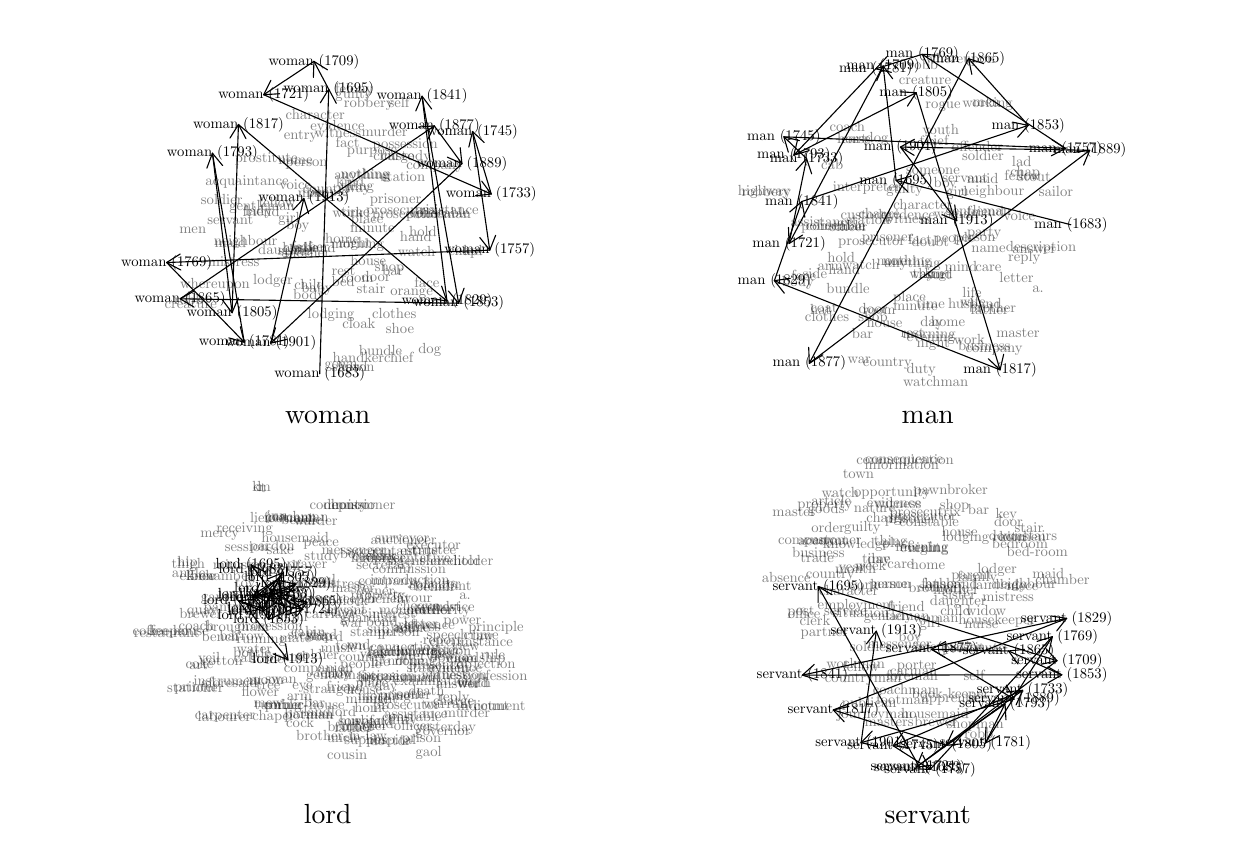
\begin{tikzpicture}[x=1pt,y=1pt]
\definecolor{fillColor}{RGB}{255,255,255}
\path[use as bounding box,fill=fillColor,fill opacity=0.00] (0,0) rectangle (433.62,289.08);
\begin{scope}
\path[clip] (  0.00,  0.00) rectangle (433.62,289.08);
\definecolor{drawColor}{RGB}{0,0,0}

\node[text=drawColor,anchor=base,inner sep=0pt, outer sep=0pt, scale=  0.53] at (105.52,162.68) {woman (1683)};

\node[text=drawColor,anchor=base,inner sep=0pt, outer sep=0pt, scale=  0.53] at (108.79,265.52) {woman (1695)};

\node[text=drawColor,anchor=base,inner sep=0pt, outer sep=0pt, scale=  0.53] at (103.44,275.58) {woman (1709)};

\node[text=drawColor,anchor=base,inner sep=0pt, outer sep=0pt, scale=  0.53] at ( 85.29,263.53) {woman (1721)};

\node[text=drawColor,anchor=base,inner sep=0pt, outer sep=0pt, scale=  0.53] at (167.51,227.65) {woman (1733)};

\node[text=drawColor,anchor=base,inner sep=0pt, outer sep=0pt, scale=  0.53] at (160.74,250.24) {woman (1745)};

\node[text=drawColor,anchor=base,inner sep=0pt, outer sep=0pt, scale=  0.53] at (166.97,207.37) {woman (1757)};

\node[text=drawColor,anchor=base,inner sep=0pt, outer sep=0pt, scale=  0.53] at ( 50.21,202.89) {woman (1769)};

\node[text=drawColor,anchor=base,inner sep=0pt, outer sep=0pt, scale=  0.53] at ( 78.26,174.09) {woman (1781)};

\node[text=drawColor,anchor=base,inner sep=0pt, outer sep=0pt, scale=  0.53] at ( 66.76,242.39) {woman (1793)};

\node[text=drawColor,anchor=base,inner sep=0pt, outer sep=0pt, scale=  0.53] at ( 73.85,184.76) {woman (1805)};

\node[text=drawColor,anchor=base,inner sep=0pt, outer sep=0pt, scale=  0.53] at ( 76.16,252.77) {woman (1817)};

\node[text=drawColor,anchor=base,inner sep=0pt, outer sep=0pt, scale=  0.53] at (151.52,188.93) {woman (1829)};

\node[text=drawColor,anchor=base,inner sep=0pt, outer sep=0pt, scale=  0.53] at (142.51,262.98) {woman (1841)};

\node[text=drawColor,anchor=base,inner sep=0pt, outer sep=0pt, scale=  0.53] at (155.73,188.19) {woman (1853)};

\node[text=drawColor,anchor=base,inner sep=0pt, outer sep=0pt, scale=  0.53] at ( 55.10,189.79) {woman (1865)};

\node[text=drawColor,anchor=base,inner sep=0pt, outer sep=0pt, scale=  0.53] at (146.94,252.26) {woman (1877)};

\node[text=drawColor,anchor=base,inner sep=0pt, outer sep=0pt, scale=  0.53] at (156.92,238.63) {woman (1889)};

\node[text=drawColor,anchor=base,inner sep=0pt, outer sep=0pt, scale=  0.53] at ( 87.87,173.77) {woman (1901)};

\node[text=drawColor,anchor=base,inner sep=0pt, outer sep=0pt, scale=  0.53] at ( 99.80,226.09) {woman (1913)};
\definecolor{drawColor}{RGB}{0,0,0}

\node[text=drawColor,text opacity=0.50,anchor=base,inner sep=0pt, outer sep=0pt, scale=  0.53] at (102.67,227.62) {man};

\node[text=drawColor,text opacity=0.50,anchor=base,inner sep=0pt, outer sep=0pt, scale=  0.53] at (100.76,239.05) {person};

\node[text=drawColor,text opacity=0.50,anchor=base,inner sep=0pt, outer sep=0pt, scale=  0.53] at (101.68,207.79) {husband};

\node[text=drawColor,text opacity=0.50,anchor=base,inner sep=0pt, outer sep=0pt, scale=  0.53] at ( 73.26,209.58) {maid};

\node[text=drawColor,text opacity=0.50,anchor=base,inner sep=0pt, outer sep=0pt, scale=  0.53] at ( 59.64,214.85) {men};

\node[text=drawColor,text opacity=0.50,anchor=base,inner sep=0pt, outer sep=0pt, scale=  0.53] at (147.17,237.93) {company};

\node[text=drawColor,text opacity=0.50,anchor=base,inner sep=0pt, outer sep=0pt, scale=  0.53] at (140.27,211.96) {hand};

\node[text=drawColor,text opacity=0.50,anchor=base,inner sep=0pt, outer sep=0pt, scale=  0.53] at ( 90.10,224.00) {fellow};

\node[text=drawColor,text opacity=0.50,anchor=base,inner sep=0pt, outer sep=0pt, scale=  0.53] at (100.42,207.86) {wife};

\node[text=drawColor,text opacity=0.50,anchor=base,inner sep=0pt, outer sep=0pt, scale=  0.53] at (101.88,194.36) {child};

\node[text=drawColor,text opacity=0.50,anchor=base,inner sep=0pt, outer sep=0pt, scale=  0.53] at ( 96.75,239.77) {name};

\node[text=drawColor,text opacity=0.50,anchor=base,inner sep=0pt, outer sep=0pt, scale=  0.53] at (119.03,197.07) {room};

\node[text=drawColor,text opacity=0.50,anchor=base,inner sep=0pt, outer sep=0pt, scale=  0.53] at ( 67.66,194.91) {whereupon};

\node[text=drawColor,text opacity=0.50,anchor=base,inner sep=0pt, outer sep=0pt, scale=  0.53] at (101.03,206.16) {mother};

\node[text=drawColor,text opacity=0.50,anchor=base,inner sep=0pt, outer sep=0pt, scale=  0.53] at (112.09,249.54) {witness};

\node[text=drawColor,text opacity=0.50,anchor=base,inner sep=0pt, outer sep=0pt, scale=  0.53] at (132.95,225.37) {prisoner};

\node[text=drawColor,text opacity=0.50,anchor=base,inner sep=0pt, outer sep=0pt, scale=  0.53] at ( 94.47,218.75) {girl};

\node[text=drawColor,text opacity=0.50,anchor=base,inner sep=0pt, outer sep=0pt, scale=  0.53] at (114.12,199.67) {rest};

\node[text=drawColor,text opacity=0.50,anchor=base,inner sep=0pt, outer sep=0pt, scale=  0.53] at (123.08,203.31) {house};

\node[text=drawColor,text opacity=0.50,anchor=base,inner sep=0pt, outer sep=0pt, scale=  0.53] at (116.57,231.84) {kind};

\node[text=drawColor,text opacity=0.50,anchor=base,inner sep=0pt, outer sep=0pt, scale=  0.53] at (117.97,265.33) {felony};

\node[text=drawColor,text opacity=0.50,anchor=base,inner sep=0pt, outer sep=0pt, scale=  0.53] at (108.28,229.25) {country};

\node[text=drawColor,text opacity=0.50,anchor=base,inner sep=0pt, outer sep=0pt, scale=  0.53] at (136.53,220.25) {prosecutor};

\node[text=drawColor,text opacity=0.50,anchor=base,inner sep=0pt, outer sep=0pt, scale=  0.53] at ( 97.59,216.22) {boy};

\node[text=drawColor,text opacity=0.50,anchor=base,inner sep=0pt, outer sep=0pt, scale=  0.53] at (118.41,220.68) {time};

\node[text=drawColor,text opacity=0.50,anchor=base,inner sep=0pt, outer sep=0pt, scale=  0.53] at ( 73.23,218.01) {servant};

\node[text=drawColor,text opacity=0.50,anchor=base,inner sep=0pt, outer sep=0pt, scale=  0.53] at (134.17,260.27) {self};

\node[text=drawColor,text opacity=0.50,anchor=base,inner sep=0pt, outer sep=0pt, scale=  0.53] at (109.66,183.92) {lodging};

\node[text=drawColor,text opacity=0.50,anchor=base,inner sep=0pt, outer sep=0pt, scale=  0.53] at (119.11,230.28) {thing};

\node[text=drawColor,text opacity=0.50,anchor=base,inner sep=0pt, outer sep=0pt, scale=  0.53] at ( 84.70,223.11) {gentleman};

\node[text=drawColor,text opacity=0.50,anchor=base,inner sep=0pt, outer sep=0pt, scale=  0.53] at (111.94,251.91) {evidence};

\node[text=drawColor,text opacity=0.50,anchor=base,inner sep=0pt, outer sep=0pt, scale=  0.53] at (123.27,260.25) {robbery};

\node[text=drawColor,text opacity=0.50,anchor=base,inner sep=0pt, outer sep=0pt, scale=  0.53] at (130.81,200.99) {shop};

\node[text=drawColor,text opacity=0.50,anchor=base,inner sep=0pt, outer sep=0pt, scale=  0.53] at (122.66,218.29) {place};

\node[text=drawColor,text opacity=0.50,anchor=base,inner sep=0pt, outer sep=0pt, scale=  0.53] at (115.73,220.57) {work};

\node[text=drawColor,text opacity=0.50,anchor=base,inner sep=0pt, outer sep=0pt, scale=  0.53] at (115.60,245.94) {fact};

\node[text=drawColor,text opacity=0.50,anchor=base,inner sep=0pt, outer sep=0pt, scale=  0.53] at (117.83,263.31) {guilty};

\node[text=drawColor,text opacity=0.50,anchor=base,inner sep=0pt, outer sep=0pt, scale=  0.53] at ( 88.64,196.14) {lodger};

\node[text=drawColor,text opacity=0.50,anchor=base,inner sep=0pt, outer sep=0pt, scale=  0.53] at (113.99,195.53) {bed};

\node[text=drawColor,text opacity=0.50,anchor=base,inner sep=0pt, outer sep=0pt, scale=  0.53] at (121.93,234.64) {nothing};

\node[text=drawColor,text opacity=0.50,anchor=base,inner sep=0pt, outer sep=0pt, scale=  0.53] at ( 96.61,206.63) {sister};

\node[text=drawColor,text opacity=0.50,anchor=base,inner sep=0pt, outer sep=0pt, scale=  0.53] at (145.27,171.44) {dog};

\node[text=drawColor,text opacity=0.50,anchor=base,inner sep=0pt, outer sep=0pt, scale=  0.53] at ( 79.26,232.01) {acquaintance};

\node[text=drawColor,text opacity=0.50,anchor=base,inner sep=0pt, outer sep=0pt, scale=  0.53] at ( 78.75,210.47) {neighbour};

\node[text=drawColor,text opacity=0.50,anchor=base,inner sep=0pt, outer sep=0pt, scale=  0.53] at ( 98.65,248.73) {entry};

\node[text=drawColor,text opacity=0.50,anchor=base,inner sep=0pt, outer sep=0pt, scale=  0.53] at (124.45,243.08) {purpose};

\node[text=drawColor,text opacity=0.50,anchor=base,inner sep=0pt, outer sep=0pt, scale=  0.53] at (136.43,245.57) {possession};

\node[text=drawColor,text opacity=0.50,anchor=base,inner sep=0pt, outer sep=0pt, scale=  0.53] at ( 96.67,230.61) {voice};

\node[text=drawColor,text opacity=0.50,anchor=base,inner sep=0pt, outer sep=0pt, scale=  0.53] at ( 70.12,225.01) {soldier};

\node[text=drawColor,text opacity=0.50,anchor=base,inner sep=0pt, outer sep=0pt, scale=  0.53] at ( 93.54,207.27) {daughter};

\node[text=drawColor,text opacity=0.50,anchor=base,inner sep=0pt, outer sep=0pt, scale=  0.53] at (138.73,192.15) {orange};

\node[text=drawColor,text opacity=0.50,anchor=base,inner sep=0pt, outer sep=0pt, scale=  0.53] at (151.59,221.61) {assistance};

\node[text=drawColor,text opacity=0.50,anchor=base,inner sep=0pt, outer sep=0pt, scale=  0.53] at (160.93,206.93) {lad};

\node[text=drawColor,text opacity=0.50,anchor=base,inner sep=0pt, outer sep=0pt, scale=  0.53] at (103.94,255.90) {character};

\node[text=drawColor,text opacity=0.50,anchor=base,inner sep=0pt, outer sep=0pt, scale=  0.53] at ( 58.25,189.12) {robb};

\node[text=drawColor,text opacity=0.50,anchor=base,inner sep=0pt, outer sep=0pt, scale=  0.53] at ( 58.91,187.58) {creature};

\node[text=drawColor,text opacity=0.50,anchor=base,inner sep=0pt, outer sep=0pt, scale=  0.53] at (108.34,228.23) {people};

\node[text=drawColor,text opacity=0.50,anchor=base,inner sep=0pt, outer sep=0pt, scale=  0.53] at (119.69,180.43) {cloak};

\node[text=drawColor,text opacity=0.50,anchor=base,inner sep=0pt, outer sep=0pt, scale=  0.53] at ( 74.43,202.91) {mistress};

\node[text=drawColor,text opacity=0.50,anchor=base,inner sep=0pt, outer sep=0pt, scale=  0.53] at (118.25,209.80) {night};

\node[text=drawColor,text opacity=0.50,anchor=base,inner sep=0pt, outer sep=0pt, scale=  0.53] at (113.70,211.00) {home};

\node[text=drawColor,text opacity=0.50,anchor=base,inner sep=0pt, outer sep=0pt, scale=  0.53] at (119.42,229.35) {way};

\node[text=drawColor,text opacity=0.50,anchor=base,inner sep=0pt, outer sep=0pt, scale=  0.53] at (131.94,199.44) {bar};

\node[text=drawColor,text opacity=0.50,anchor=base,inner sep=0pt, outer sep=0pt, scale=  0.53] at (135.19,221.74) {prosecutrix};

\node[text=drawColor,text opacity=0.50,anchor=base,inner sep=0pt, outer sep=0pt, scale=  0.53] at (113.25,165.80) {gown};

\node[text=drawColor,text opacity=0.50,anchor=base,inner sep=0pt, outer sep=0pt, scale=  0.53] at (119.14,209.22) {morning};

\node[text=drawColor,text opacity=0.50,anchor=base,inner sep=0pt, outer sep=0pt, scale=  0.53] at (101.71,191.00) {body};

\node[text=drawColor,text opacity=0.50,anchor=base,inner sep=0pt, outer sep=0pt, scale=  0.53] at (124.04,193.08) {stair};

\node[text=drawColor,text opacity=0.50,anchor=base,inner sep=0pt, outer sep=0pt, scale=  0.53] at (125.93,197.30) {door};

\node[text=drawColor,text opacity=0.50,anchor=base,inner sep=0pt, outer sep=0pt, scale=  0.53] at (118.73,164.70) {apron};

\node[text=drawColor,text opacity=0.50,anchor=base,inner sep=0pt, outer sep=0pt, scale=  0.53] at ( 83.48,221.07) {lady};

\node[text=drawColor,text opacity=0.50,anchor=base,inner sep=0pt, outer sep=0pt, scale=  0.53] at (134.55,178.57) {shoe};

\node[text=drawColor,text opacity=0.50,anchor=base,inner sep=0pt, outer sep=0pt, scale=  0.53] at (132.47,184.08) {clothes};

\node[text=drawColor,text opacity=0.50,anchor=base,inner sep=0pt, outer sep=0pt, scale=  0.53] at (136.75,241.16) {custody};

\node[text=drawColor,text opacity=0.50,anchor=base,inner sep=0pt, outer sep=0pt, scale=  0.53] at (124.79,168.27) {handkerchief};

\node[text=drawColor,text opacity=0.50,anchor=base,inner sep=0pt, outer sep=0pt, scale=  0.53] at (140.50,206.45) {watch};

\node[text=drawColor,text opacity=0.50,anchor=base,inner sep=0pt, outer sep=0pt, scale=  0.53] at (127.51,170.66) {bundle};

\node[text=drawColor,text opacity=0.50,anchor=base,inner sep=0pt, outer sep=0pt, scale=  0.53] at (116.32,164.74) {shawl};

\node[text=drawColor,text opacity=0.50,anchor=base,inner sep=0pt, outer sep=0pt, scale=  0.53] at (132.33,241.08) {charge};

\node[text=drawColor,text opacity=0.50,anchor=base,inner sep=0pt, outer sep=0pt, scale=  0.53] at (148.50,220.21) {policeman};

\node[text=drawColor,text opacity=0.50,anchor=base,inner sep=0pt, outer sep=0pt, scale=  0.53] at (142.85,213.73) {hold};

\node[text=drawColor,text opacity=0.50,anchor=base,inner sep=0pt, outer sep=0pt, scale=  0.53] at ( 84.37,220.82) {friend};

\node[text=drawColor,text opacity=0.50,anchor=base,inner sep=0pt, outer sep=0pt, scale=  0.53] at (148.85,220.62) {constable};

\node[text=drawColor,text opacity=0.50,anchor=base,inner sep=0pt, outer sep=0pt, scale=  0.53] at (157.41,206.61) {chap};

\node[text=drawColor,text opacity=0.50,anchor=base,inner sep=0pt, outer sep=0pt, scale=  0.53] at (120.95,234.11) {anything};

\node[text=drawColor,text opacity=0.50,anchor=base,inner sep=0pt, outer sep=0pt, scale=  0.53] at (102.03,208.37) {father};

\node[text=drawColor,text opacity=0.50,anchor=base,inner sep=0pt, outer sep=0pt, scale=  0.53] at (144.25,195.28) {face};

\node[text=drawColor,text opacity=0.50,anchor=base,inner sep=0pt, outer sep=0pt, scale=  0.53] at ( 86.21,240.39) {prostitute};

\node[text=drawColor,text opacity=0.50,anchor=base,inner sep=0pt, outer sep=0pt, scale=  0.53] at (104.48,193.51) {baby};

\node[text=drawColor,text opacity=0.50,anchor=base,inner sep=0pt, outer sep=0pt, scale=  0.53] at (128.98,249.88) {murder};

\node[text=drawColor,text opacity=0.50,anchor=base,inner sep=0pt, outer sep=0pt, scale=  0.53] at (124.58,215.12) {minute};

\node[text=drawColor,text opacity=0.50,anchor=base,inner sep=0pt, outer sep=0pt, scale=  0.53] at (135.67,233.34) {station};
\definecolor{drawColor}{RGB}{0,0,0}

\path[draw=drawColor,line width= 0.4pt,line join=round,line cap=round] (105.52,164.00) -- (108.79,266.84);

\path[draw=drawColor,line width= 0.4pt,line join=round,line cap=round] (111.52,261.74) --
	(108.79,266.84) --
	(105.75,261.92);

\path[draw=drawColor,line width= 0.4pt,line join=round,line cap=round] (108.79,266.84) -- (103.44,276.90);

\path[draw=drawColor,line width= 0.4pt,line join=round,line cap=round] (108.34,273.84) --
	(103.44,276.90) --
	(103.24,271.13);

\path[draw=drawColor,line width= 0.4pt,line join=round,line cap=round] (103.44,276.90) -- ( 85.29,264.85);

\path[draw=drawColor,line width= 0.4pt,line join=round,line cap=round] ( 87.86,270.03) --
	( 85.29,264.85) --
	( 91.06,265.21);

\path[draw=drawColor,line width= 0.4pt,line join=round,line cap=round] ( 85.29,264.85) -- (167.51,228.97);

\path[draw=drawColor,line width= 0.4pt,line join=round,line cap=round] (161.76,228.32) --
	(167.51,228.97) --
	(164.07,233.62);

\path[draw=drawColor,line width= 0.4pt,line join=round,line cap=round] (167.51,228.97) -- (160.74,251.56);

\path[draw=drawColor,line width= 0.4pt,line join=round,line cap=round] (164.95,247.59) --
	(160.74,251.56) --
	(159.41,245.93);

\path[draw=drawColor,line width= 0.4pt,line join=round,line cap=round] (160.74,251.56) -- (166.97,208.69);

\path[draw=drawColor,line width= 0.4pt,line join=round,line cap=round] (163.39,213.23) --
	(166.97,208.69) --
	(169.11,214.06);

\path[draw=drawColor,line width= 0.4pt,line join=round,line cap=round] (166.97,208.69) -- ( 50.21,204.21);

\path[draw=drawColor,line width= 0.4pt,line join=round,line cap=round] ( 55.11,207.29) --
	( 50.21,204.21) --
	( 55.33,201.51);

\path[draw=drawColor,line width= 0.4pt,line join=round,line cap=round] ( 50.21,204.21) -- ( 78.26,175.41);

\path[draw=drawColor,line width= 0.4pt,line join=round,line cap=round] ( 72.69,176.98) --
	( 78.26,175.41) --
	( 76.84,181.01);

\path[draw=drawColor,line width= 0.4pt,line join=round,line cap=round] ( 78.26,175.41) -- ( 66.76,243.71);

\path[draw=drawColor,line width= 0.4pt,line join=round,line cap=round] ( 70.45,239.25) --
	( 66.76,243.71) --
	( 64.74,238.29);

\path[draw=drawColor,line width= 0.4pt,line join=round,line cap=round] ( 66.76,243.71) -- ( 73.85,186.08);

\path[draw=drawColor,line width= 0.4pt,line join=round,line cap=round] ( 70.37,190.70) --
	( 73.85,186.08) --
	( 76.10,191.40);

\path[draw=drawColor,line width= 0.4pt,line join=round,line cap=round] ( 73.85,186.08) -- ( 76.16,254.09);

\path[draw=drawColor,line width= 0.4pt,line join=round,line cap=round] ( 78.88,248.98) --
	( 76.16,254.09) --
	( 73.10,249.18);

\path[draw=drawColor,line width= 0.4pt,line join=round,line cap=round] ( 76.16,254.09) -- (151.52,190.25);

\path[draw=drawColor,line width= 0.4pt,line join=round,line cap=round] (145.83,191.28) --
	(151.52,190.25) --
	(149.57,195.69);

\path[draw=drawColor,line width= 0.4pt,line join=round,line cap=round] (151.52,190.25) -- (142.51,264.30);

\path[draw=drawColor,line width= 0.4pt,line join=round,line cap=round] (145.98,259.68) --
	(142.51,264.30) --
	(140.24,258.98);

\path[draw=drawColor,line width= 0.4pt,line join=round,line cap=round] (142.51,264.30) -- (155.73,189.51);

\path[draw=drawColor,line width= 0.4pt,line join=round,line cap=round] (152.01,193.94) --
	(155.73,189.51) --
	(157.70,194.94);

\path[draw=drawColor,line width= 0.4pt,line join=round,line cap=round] (155.73,189.51) -- ( 55.10,191.11);

\path[draw=drawColor,line width= 0.4pt,line join=round,line cap=round] ( 60.16,193.93) --
	( 55.10,191.11) --
	( 60.06,188.14);

\path[draw=drawColor,line width= 0.4pt,line join=round,line cap=round] ( 55.10,191.11) -- (146.94,253.58);

\path[draw=drawColor,line width= 0.4pt,line join=round,line cap=round] (144.42,248.37) --
	(146.94,253.58) --
	(141.17,253.15);

\path[draw=drawColor,line width= 0.4pt,line join=round,line cap=round] (146.94,253.58) -- (156.92,239.95);

\path[draw=drawColor,line width= 0.4pt,line join=round,line cap=round] (151.63,242.29) --
	(156.92,239.95) --
	(156.29,245.70);

\path[draw=drawColor,line width= 0.4pt,line join=round,line cap=round] (156.92,239.95) -- ( 87.87,175.09);

\path[draw=drawColor,line width= 0.4pt,line join=round,line cap=round] ( 89.54,180.63) --
	( 87.87,175.09) --
	( 93.50,176.41);

\path[draw=drawColor,line width= 0.4pt,line join=round,line cap=round] ( 87.87,175.09) -- ( 99.80,227.41);

\path[draw=drawColor,line width= 0.4pt,line join=round,line cap=round] (101.50,221.89) --
	( 99.80,227.41) --
	( 95.87,223.17);

\node[text=drawColor,anchor=base,inner sep=0pt, outer sep=0pt, scale=  1.00] at (108.41,146.12) {woman};
\end{scope}
\begin{scope}
\path[clip] (  0.00,  0.00) rectangle (433.62,289.08);
\definecolor{drawColor}{RGB}{0,0,0}

\node[text=drawColor,anchor=base,inner sep=0pt, outer sep=0pt, scale=  0.53] at (376.95,216.55) {man (1683)};

\node[text=drawColor,anchor=base,inner sep=0pt, outer sep=0pt, scale=  0.53] at (313.81,232.58) {man (1695)};

\node[text=drawColor,anchor=base,inner sep=0pt, outer sep=0pt, scale=  0.53] at (309.12,273.93) {man (1709)};

\node[text=drawColor,anchor=base,inner sep=0pt, outer sep=0pt, scale=  0.53] at (275.13,209.76) {man (1721)};

\node[text=drawColor,anchor=base,inner sep=0pt, outer sep=0pt, scale=  0.53] at (281.46,240.45) {man (1733)};

\node[text=drawColor,anchor=base,inner sep=0pt, outer sep=0pt, scale=  0.53] at (273.25,248.32) {man (1745)};

\node[text=drawColor,anchor=base,inner sep=0pt, outer sep=0pt, scale=  0.53] at (375.02,244.14) {man (1757)};

\node[text=drawColor,anchor=base,inner sep=0pt, outer sep=0pt, scale=  0.53] at (323.24,278.13) {man (1769)};

\node[text=drawColor,anchor=base,inner sep=0pt, outer sep=0pt, scale=  0.53] at (306.46,272.89) {man (1781)};

\node[text=drawColor,anchor=base,inner sep=0pt, outer sep=0pt, scale=  0.53] at (276.86,241.70) {man (1793)};

\node[text=drawColor,anchor=base,inner sep=0pt, outer sep=0pt, scale=  0.53] at (321.05,264.26) {man (1805)};

\node[text=drawColor,anchor=base,inner sep=0pt, outer sep=0pt, scale=  0.53] at (351.37,164.12) {man (1817)};

\node[text=drawColor,anchor=base,inner sep=0pt, outer sep=0pt, scale=  0.53] at (269.82,196.33) {man (1829)};

\node[text=drawColor,anchor=base,inner sep=0pt, outer sep=0pt, scale=  0.53] at (279.74,224.94) {man (1841)};

\node[text=drawColor,anchor=base,inner sep=0pt, outer sep=0pt, scale=  0.53] at (361.55,252.46) {man (1853)};

\node[text=drawColor,anchor=base,inner sep=0pt, outer sep=0pt, scale=  0.53] at (339.98,276.56) {man (1865)};

\node[text=drawColor,anchor=base,inner sep=0pt, outer sep=0pt, scale=  0.53] at (282.45,166.48) {man (1877)};

\node[text=drawColor,anchor=base,inner sep=0pt, outer sep=0pt, scale=  0.53] at (383.77,243.44) {man (1889)};

\node[text=drawColor,anchor=base,inner sep=0pt, outer sep=0pt, scale=  0.53] at (315.37,244.61) {man (1901)};

\node[text=drawColor,anchor=base,inner sep=0pt, outer sep=0pt, scale=  0.53] at (335.74,217.98) {man (1913)};
\definecolor{drawColor}{RGB}{0,0,0}

\node[text=drawColor,text opacity=0.50,anchor=base,inner sep=0pt, outer sep=0pt, scale=  0.53] at (335.46,220.14) {woman};

\node[text=drawColor,text opacity=0.50,anchor=base,inner sep=0pt, outer sep=0pt, scale=  0.53] at (346.42,260.56) {men};

\node[text=drawColor,text opacity=0.50,anchor=base,inner sep=0pt, outer sep=0pt, scale=  0.53] at (342.10,211.70) {person};

\node[text=drawColor,text opacity=0.50,anchor=base,inner sep=0pt, outer sep=0pt, scale=  0.53] at (359.56,233.98) {fellow};

\node[text=drawColor,text opacity=0.50,anchor=base,inner sep=0pt, outer sep=0pt, scale=  0.53] at (349.20,171.67) {company};

\node[text=drawColor,text opacity=0.50,anchor=base,inner sep=0pt, outer sep=0pt, scale=  0.53] at (317.73,218.14) {witness};

\node[text=drawColor,text opacity=0.50,anchor=base,inner sep=0pt, outer sep=0pt, scale=  0.53] at (331.60,231.39) {boy};

\node[text=drawColor,text opacity=0.50,anchor=base,inner sep=0pt, outer sep=0pt, scale=  0.53] at (329.92,250.41) {youth};

\node[text=drawColor,text opacity=0.50,anchor=base,inner sep=0pt, outer sep=0pt, scale=  0.53] at (334.68,211.46) {people};

\node[text=drawColor,text opacity=0.50,anchor=base,inner sep=0pt, outer sep=0pt, scale=  0.53] at (345.10,232.86) {maid};

\node[text=drawColor,text opacity=0.50,anchor=base,inner sep=0pt, outer sep=0pt, scale=  0.53] at (343.44,221.16) {gentleman};

\node[text=drawColor,text opacity=0.50,anchor=base,inner sep=0pt, outer sep=0pt, scale=  0.53] at (310.68,166.69) {country};

\node[text=drawColor,text opacity=0.50,anchor=base,inner sep=0pt, outer sep=0pt, scale=  0.53] at (266.98,228.14) {robbery};

\node[text=drawColor,text opacity=0.50,anchor=base,inner sep=0pt, outer sep=0pt, scale=  0.53] at (319.76,176.98) {rest};

\node[text=drawColor,text opacity=0.50,anchor=base,inner sep=0pt, outer sep=0pt, scale=  0.53] at (347.20,207.73) {name};

\node[text=drawColor,text opacity=0.50,anchor=base,inner sep=0pt, outer sep=0pt, scale=  0.53] at (327.51,246.68) {thief};

\node[text=drawColor,text opacity=0.50,anchor=base,inner sep=0pt, outer sep=0pt, scale=  0.53] at (326.27,187.71) {time};

\node[text=drawColor,text opacity=0.50,anchor=base,inner sep=0pt, outer sep=0pt, scale=  0.53] at (338.76,233.16) {servant};

\node[text=drawColor,text opacity=0.50,anchor=base,inner sep=0pt, outer sep=0pt, scale=  0.53] at (295.10,199.98) {hand};

\node[text=drawColor,text opacity=0.50,anchor=base,inner sep=0pt, outer sep=0pt, scale=  0.53] at (341.24,191.55) {life};

\node[text=drawColor,text opacity=0.50,anchor=base,inner sep=0pt, outer sep=0pt, scale=  0.53] at (326.28,175.73) {evening};

\node[text=drawColor,text opacity=0.50,anchor=base,inner sep=0pt, outer sep=0pt, scale=  0.53] at (316.90,228.98) {guilty};

\node[text=drawColor,text opacity=0.50,anchor=base,inner sep=0pt, outer sep=0pt, scale=  0.53] at (296.17,251.64) {coach};

\node[text=drawColor,text opacity=0.50,anchor=base,inner sep=0pt, outer sep=0pt, scale=  0.53] at (304.99,210.51) {prosecutor};

\node[text=drawColor,text opacity=0.50,anchor=base,inner sep=0pt, outer sep=0pt, scale=  0.53] at (266.09,228.50) {highway};

\node[text=drawColor,text opacity=0.50,anchor=base,inner sep=0pt, outer sep=0pt, scale=  0.53] at (307.72,220.14) {charge};

\node[text=drawColor,text opacity=0.50,anchor=base,inner sep=0pt, outer sep=0pt, scale=  0.53] at (307.65,185.31) {room};

\node[text=drawColor,text opacity=0.50,anchor=base,inner sep=0pt, outer sep=0pt, scale=  0.53] at (345.62,213.69) {party};

\node[text=drawColor,text opacity=0.50,anchor=base,inner sep=0pt, outer sep=0pt, scale=  0.53] at (325.84,198.41) {thing};

\node[text=drawColor,text opacity=0.50,anchor=base,inner sep=0pt, outer sep=0pt, scale=  0.53] at (287.07,217.15) {assistance};

\node[text=drawColor,text opacity=0.50,anchor=base,inner sep=0pt, outer sep=0pt, scale=  0.53] at (298.56,247.32) {horse};

\node[text=drawColor,text opacity=0.50,anchor=base,inner sep=0pt, outer sep=0pt, scale=  0.53] at (310.73,211.67) {prisoner};

\node[text=drawColor,text opacity=0.50,anchor=base,inner sep=0pt, outer sep=0pt, scale=  0.53] at (335.77,227.96) {girl};

\node[text=drawColor,text opacity=0.50,anchor=base,inner sep=0pt, outer sep=0pt, scale=  0.53] at (306.94,247.76) {dog};

\node[text=drawColor,text opacity=0.50,anchor=base,inner sep=0pt, outer sep=0pt, scale=  0.53] at (290.01,201.18) {arm};

\node[text=drawColor,text opacity=0.50,anchor=base,inner sep=0pt, outer sep=0pt, scale=  0.53] at (323.11,198.30) {way};

\node[text=drawColor,text opacity=0.50,anchor=base,inner sep=0pt, outer sep=0pt, scale=  0.53] at (318.10,219.74) {evidence};

\node[text=drawColor,text opacity=0.50,anchor=base,inner sep=0pt, outer sep=0pt, scale=  0.53] at (312.25,203.22) {none};

\node[text=drawColor,text opacity=0.50,anchor=base,inner sep=0pt, outer sep=0pt, scale=  0.53] at (286.59,185.51) {hat};

\node[text=drawColor,text opacity=0.50,anchor=base,inner sep=0pt, outer sep=0pt, scale=  0.53] at (337.03,276.08) {whereupon};

\node[text=drawColor,text opacity=0.50,anchor=base,inner sep=0pt, outer sep=0pt, scale=  0.53] at (343.19,244.49) {offender};

\node[text=drawColor,text opacity=0.50,anchor=base,inner sep=0pt, outer sep=0pt, scale=  0.53] at (303.23,229.73) {interpreter};

\node[text=drawColor,text opacity=0.50,anchor=base,inner sep=0pt, outer sep=0pt, scale=  0.53] at (323.67,273.91) {robb};

\node[text=drawColor,text opacity=0.50,anchor=base,inner sep=0pt, outer sep=0pt, scale=  0.53] at (323.49,223.22) {character};

\node[text=drawColor,text opacity=0.50,anchor=base,inner sep=0pt, outer sep=0pt, scale=  0.53] at (345.18,241.07) {soldier};

\node[text=drawColor,text opacity=0.50,anchor=base,inner sep=0pt, outer sep=0pt, scale=  0.53] at (346.17,220.67) {friend};

\node[text=drawColor,text opacity=0.50,anchor=base,inner sep=0pt, outer sep=0pt, scale=  0.53] at (328.09,159.57) {watchman};

\node[text=drawColor,text opacity=0.50,anchor=base,inner sep=0pt, outer sep=0pt, scale=  0.53] at (322.49,210.61) {fact};

\node[text=drawColor,text opacity=0.50,anchor=base,inner sep=0pt, outer sep=0pt, scale=  0.53] at (348.64,228.61) {neighbour};

\node[text=drawColor,text opacity=0.50,anchor=base,inner sep=0pt, outer sep=0pt, scale=  0.53] at (322.88,164.13) {duty};

\node[text=drawColor,text opacity=0.50,anchor=base,inner sep=0pt, outer sep=0pt, scale=  0.53] at (342.30,187.61) {husband};

\node[text=drawColor,text opacity=0.50,anchor=base,inner sep=0pt, outer sep=0pt, scale=  0.53] at (360.11,204.54) {reply};

\node[text=drawColor,text opacity=0.50,anchor=base,inner sep=0pt, outer sep=0pt, scale=  0.53] at (357.34,196.95) {letter};

\node[text=drawColor,text opacity=0.50,anchor=base,inner sep=0pt, outer sep=0pt, scale=  0.53] at (363.72,207.38) {answer};

\node[text=drawColor,text opacity=0.50,anchor=base,inner sep=0pt, outer sep=0pt, scale=  0.53] at (358.30,219.45) {voice};

\node[text=drawColor,text opacity=0.50,anchor=base,inner sep=0pt, outer sep=0pt, scale=  0.53] at (359.21,239.00) {lad};

\node[text=drawColor,text opacity=0.50,anchor=base,inner sep=0pt, outer sep=0pt, scale=  0.53] at (330.76,259.70) {rogue};

\node[text=drawColor,text opacity=0.50,anchor=base,inner sep=0pt, outer sep=0pt, scale=  0.53] at (348.66,186.07) {brother};

\node[text=drawColor,text opacity=0.50,anchor=base,inner sep=0pt, outer sep=0pt, scale=  0.53] at (278.36,195.57) {body};

\node[text=drawColor,text opacity=0.50,anchor=base,inner sep=0pt, outer sep=0pt, scale=  0.53] at (371.56,227.98) {sailor};

\node[text=drawColor,text opacity=0.50,anchor=base,inner sep=0pt, outer sep=0pt, scale=  0.53] at (357.82,177.16) {master};

\node[text=drawColor,text opacity=0.50,anchor=base,inner sep=0pt, outer sep=0pt, scale=  0.53] at (347.13,200.84) {care};

\node[text=drawColor,text opacity=0.50,anchor=base,inner sep=0pt, outer sep=0pt, scale=  0.53] at (341.56,188.34) {wife};

\node[text=drawColor,text opacity=0.50,anchor=base,inner sep=0pt, outer sep=0pt, scale=  0.53] at (347.63,185.40) {father};

\node[text=drawColor,text opacity=0.50,anchor=base,inner sep=0pt, outer sep=0pt, scale=  0.53] at (324.23,268.57) {creature};

\node[text=drawColor,text opacity=0.50,anchor=base,inner sep=0pt, outer sep=0pt, scale=  0.53] at (300.50,167.55) {war};

\node[text=drawColor,text opacity=0.50,anchor=base,inner sep=0pt, outer sep=0pt, scale=  0.53] at (287.80,186.29) {coat};

\node[text=drawColor,text opacity=0.50,anchor=base,inner sep=0pt, outer sep=0pt, scale=  0.53] at (332.55,181.12) {home};

\node[text=drawColor,text opacity=0.50,anchor=base,inner sep=0pt, outer sep=0pt, scale=  0.53] at (309.62,180.76) {house};

\node[text=drawColor,text opacity=0.50,anchor=base,inner sep=0pt, outer sep=0pt, scale=  0.53] at (301.11,201.59) {watch};

\node[text=drawColor,text opacity=0.50,anchor=base,inner sep=0pt, outer sep=0pt, scale=  0.53] at (325.76,176.65) {morning};

\node[text=drawColor,text opacity=0.50,anchor=base,inner sep=0pt, outer sep=0pt, scale=  0.53] at (301.68,176.67) {bar};

\node[text=drawColor,text opacity=0.50,anchor=base,inner sep=0pt, outer sep=0pt, scale=  0.53] at (340.27,174.69) {work};

\node[text=drawColor,text opacity=0.50,anchor=base,inner sep=0pt, outer sep=0pt, scale=  0.53] at (329.42,198.03) {sort};

\node[text=drawColor,text opacity=0.50,anchor=base,inner sep=0pt, outer sep=0pt, scale=  0.53] at (346.85,260.36) {working};

\node[text=drawColor,text opacity=0.50,anchor=base,inner sep=0pt, outer sep=0pt, scale=  0.53] at (345.69,172.43) {business};

\node[text=drawColor,text opacity=0.50,anchor=base,inner sep=0pt, outer sep=0pt, scale=  0.53] at (326.66,181.09) {day};

\node[text=drawColor,text opacity=0.50,anchor=base,inner sep=0pt, outer sep=0pt, scale=  0.53] at (288.85,182.92) {clothes};

\node[text=drawColor,text opacity=0.50,anchor=base,inner sep=0pt, outer sep=0pt, scale=  0.53] at (317.85,202.96) {nothing};

\node[text=drawColor,text opacity=0.50,anchor=base,inner sep=0pt, outer sep=0pt, scale=  0.53] at (337.23,201.15) {mind};

\node[text=drawColor,text opacity=0.50,anchor=base,inner sep=0pt, outer sep=0pt, scale=  0.53] at (329.20,198.32) {kind};

\node[text=drawColor,text opacity=0.50,anchor=base,inner sep=0pt, outer sep=0pt, scale=  0.53] at (284.46,198.38) {side};

\node[text=drawColor,text opacity=0.50,anchor=base,inner sep=0pt, outer sep=0pt, scale=  0.53] at (280.43,197.83) {face};

\node[text=drawColor,text opacity=0.50,anchor=base,inner sep=0pt, outer sep=0pt, scale=  0.53] at (293.99,204.27) {hold};

\node[text=drawColor,text opacity=0.50,anchor=base,inner sep=0pt, outer sep=0pt, scale=  0.53] at (296.43,192.86) {bundle};

\node[text=drawColor,text opacity=0.50,anchor=base,inner sep=0pt, outer sep=0pt, scale=  0.53] at (327.23,173.54) {night};

\node[text=drawColor,text opacity=0.50,anchor=base,inner sep=0pt, outer sep=0pt, scale=  0.53] at (302.74,219.94) {custody};

\node[text=drawColor,text opacity=0.50,anchor=base,inner sep=0pt, outer sep=0pt, scale=  0.53] at (320.78,186.74) {minute};

\node[text=drawColor,text opacity=0.50,anchor=base,inner sep=0pt, outer sep=0pt, scale=  0.53] at (298.71,247.06) {cart};

\node[text=drawColor,text opacity=0.50,anchor=base,inner sep=0pt, outer sep=0pt, scale=  0.53] at (363.78,233.46) {stout};

\node[text=drawColor,text opacity=0.50,anchor=base,inner sep=0pt, outer sep=0pt, scale=  0.53] at (365.08,193.24) {a.};

\node[text=drawColor,text opacity=0.50,anchor=base,inner sep=0pt, outer sep=0pt, scale=  0.53] at (291.16,215.69) {policeman};

\node[text=drawColor,text opacity=0.50,anchor=base,inner sep=0pt, outer sep=0pt, scale=  0.53] at (296.48,215.34) {officer};

\node[text=drawColor,text opacity=0.50,anchor=base,inner sep=0pt, outer sep=0pt, scale=  0.53] at (290.70,237.94) {cab};

\node[text=drawColor,text opacity=0.50,anchor=base,inner sep=0pt, outer sep=0pt, scale=  0.53] at (318.64,189.99) {place};

\node[text=drawColor,text opacity=0.50,anchor=base,inner sep=0pt, outer sep=0pt, scale=  0.53] at (319.76,202.57) {anything};

\node[text=drawColor,text opacity=0.50,anchor=base,inner sep=0pt, outer sep=0pt, scale=  0.53] at (360.48,235.47) {chap};

\node[text=drawColor,text opacity=0.50,anchor=base,inner sep=0pt, outer sep=0pt, scale=  0.53] at (291.93,215.68) {constable};

\node[text=drawColor,text opacity=0.50,anchor=base,inner sep=0pt, outer sep=0pt, scale=  0.53] at (366.20,208.20) {description};

\node[text=drawColor,text opacity=0.50,anchor=base,inner sep=0pt, outer sep=0pt, scale=  0.53] at (326.20,210.07) {doubt};

\node[text=drawColor,text opacity=0.50,anchor=base,inner sep=0pt, outer sep=0pt, scale=  0.53] at (303.76,217.95) {station};

\node[text=drawColor,text opacity=0.50,anchor=base,inner sep=0pt, outer sep=0pt, scale=  0.53] at (305.46,182.77) {shop};

\node[text=drawColor,text opacity=0.50,anchor=base,inner sep=0pt, outer sep=0pt, scale=  0.53] at (305.54,185.77) {door};

\node[text=drawColor,text opacity=0.50,anchor=base,inner sep=0pt, outer sep=0pt, scale=  0.53] at (327.13,236.06) {someone};
\definecolor{drawColor}{RGB}{0,0,0}

\path[draw=drawColor,line width= 0.4pt,line join=round,line cap=round] (376.95,217.87) -- (313.81,233.90);

\path[draw=drawColor,line width= 0.4pt,line join=round,line cap=round] (319.38,235.47) --
	(313.81,233.90) --
	(317.96,229.87);

\path[draw=drawColor,line width= 0.4pt,line join=round,line cap=round] (313.81,233.90) -- (309.12,275.25);

\path[draw=drawColor,line width= 0.4pt,line join=round,line cap=round] (312.56,270.60) --
	(309.12,275.25) --
	(306.81,269.95);

\path[draw=drawColor,line width= 0.4pt,line join=round,line cap=round] (309.12,275.25) -- (275.13,211.08);

\path[draw=drawColor,line width= 0.4pt,line join=round,line cap=round] (274.92,216.86) --
	(275.13,211.08) --
	(280.02,214.15);

\path[draw=drawColor,line width= 0.4pt,line join=round,line cap=round] (275.13,211.08) -- (281.46,241.77);

\path[draw=drawColor,line width= 0.4pt,line join=round,line cap=round] (283.27,236.28) --
	(281.46,241.77) --
	(277.61,237.45);

\path[draw=drawColor,line width= 0.4pt,line join=round,line cap=round] (281.46,241.77) -- (273.25,249.64);

\path[draw=drawColor,line width= 0.4pt,line join=round,line cap=round] (278.86,248.26) --
	(273.25,249.64) --
	(274.86,244.09);

\path[draw=drawColor,line width= 0.4pt,line join=round,line cap=round] (273.25,249.64) -- (375.02,245.46);

\path[draw=drawColor,line width= 0.4pt,line join=round,line cap=round] (369.90,242.78) --
	(375.02,245.46) --
	(370.14,248.56);

\path[draw=drawColor,line width= 0.4pt,line join=round,line cap=round] (375.02,245.46) -- (323.24,279.45);

\path[draw=drawColor,line width= 0.4pt,line join=round,line cap=round] (329.01,279.12) --
	(323.24,279.45) --
	(325.84,274.29);

\path[draw=drawColor,line width= 0.4pt,line join=round,line cap=round] (323.24,279.45) -- (306.46,274.21);

\path[draw=drawColor,line width= 0.4pt,line join=round,line cap=round] (310.38,278.46) --
	(306.46,274.21) --
	(312.10,272.94);

\path[draw=drawColor,line width= 0.4pt,line join=round,line cap=round] (306.46,274.21) -- (276.86,243.02);

\path[draw=drawColor,line width= 0.4pt,line join=round,line cap=round] (278.21,248.64) --
	(276.86,243.02) --
	(282.40,244.66);

\path[draw=drawColor,line width= 0.4pt,line join=round,line cap=round] (276.86,243.02) -- (321.05,265.58);

\path[draw=drawColor,line width= 0.4pt,line join=round,line cap=round] (317.90,260.73) --
	(321.05,265.58) --
	(315.27,265.88);

\path[draw=drawColor,line width= 0.4pt,line join=round,line cap=round] (321.05,265.58) -- (351.37,165.44);

\path[draw=drawColor,line width= 0.4pt,line join=round,line cap=round] (347.15,169.40) --
	(351.37,165.44) --
	(352.68,171.07);

\path[draw=drawColor,line width= 0.4pt,line join=round,line cap=round] (351.37,165.44) -- (269.82,197.65);

\path[draw=drawColor,line width= 0.4pt,line join=round,line cap=round] (275.54,198.50) --
	(269.82,197.65) --
	(273.42,193.13);

\path[draw=drawColor,line width= 0.4pt,line join=round,line cap=round] (269.82,197.65) -- (279.74,226.26);

\path[draw=drawColor,line width= 0.4pt,line join=round,line cap=round] (280.83,220.58) --
	(279.74,226.26) --
	(275.37,222.48);

\path[draw=drawColor,line width= 0.4pt,line join=round,line cap=round] (279.74,226.26) -- (361.55,253.78);

\path[draw=drawColor,line width= 0.4pt,line join=round,line cap=round] (357.72,249.45) --
	(361.55,253.78) --
	(355.88,254.93);

\path[draw=drawColor,line width= 0.4pt,line join=round,line cap=round] (361.55,253.78) -- (339.98,277.88);

\path[draw=drawColor,line width= 0.4pt,line join=round,line cap=round] (345.47,276.08) --
	(339.98,277.88) --
	(341.16,272.22);

\path[draw=drawColor,line width= 0.4pt,line join=round,line cap=round] (339.98,277.88) -- (282.45,167.80);

\path[draw=drawColor,line width= 0.4pt,line join=round,line cap=round] (282.21,173.57) --
	(282.45,167.80) --
	(287.33,170.89);

\path[draw=drawColor,line width= 0.4pt,line join=round,line cap=round] (282.45,167.80) -- (383.77,244.76);

\path[draw=drawColor,line width= 0.4pt,line join=round,line cap=round] (381.54,239.43) --
	(383.77,244.76) --
	(378.04,244.04);

\path[draw=drawColor,line width= 0.4pt,line join=round,line cap=round] (383.77,244.76) -- (315.37,245.93);

\path[draw=drawColor,line width= 0.4pt,line join=round,line cap=round] (320.42,248.74) --
	(315.37,245.93) --
	(320.32,242.95);

\path[draw=drawColor,line width= 0.4pt,line join=round,line cap=round] (315.37,245.93) -- (335.74,219.30);

\path[draw=drawColor,line width= 0.4pt,line join=round,line cap=round] (330.40,221.52) --
	(335.74,219.30) --
	(334.99,225.03);

\node[text=drawColor,anchor=base,inner sep=0pt, outer sep=0pt, scale=  1.00] at (325.22,146.12) {man};
\end{scope}
\begin{scope}
\path[clip] (  0.00,  0.00) rectangle (433.62,289.08);
\definecolor{drawColor}{RGB}{0,0,0}

\node[text=drawColor,anchor=base,inner sep=0pt, outer sep=0pt, scale=  0.53] at ( 81.83, 91.96) {lord (1683)};

\node[text=drawColor,anchor=base,inner sep=0pt, outer sep=0pt, scale=  0.53] at ( 80.71, 93.65) {lord (1695)};

\node[text=drawColor,anchor=base,inner sep=0pt, outer sep=0pt, scale=  0.53] at ( 91.91, 79.08) {lord (1709)};

\node[text=drawColor,anchor=base,inner sep=0pt, outer sep=0pt, scale=  0.53] at ( 99.44, 77.48) {lord (1721)};

\node[text=drawColor,anchor=base,inner sep=0pt, outer sep=0pt, scale=  0.53] at ( 90.36, 82.72) {lord (1733)};

\node[text=drawColor,anchor=base,inner sep=0pt, outer sep=0pt, scale=  0.53] at ( 87.45, 84.88) {lord (1745)};

\node[text=drawColor,anchor=base,inner sep=0pt, outer sep=0pt, scale=  0.53] at ( 92.02, 90.68) {lord (1757)};

\node[text=drawColor,anchor=base,inner sep=0pt, outer sep=0pt, scale=  0.53] at ( 84.97, 76.81) {lord (1769)};

\node[text=drawColor,anchor=base,inner sep=0pt, outer sep=0pt, scale=  0.53] at ( 76.18, 80.66) {lord (1781)};

\node[text=drawColor,anchor=base,inner sep=0pt, outer sep=0pt, scale=  0.53] at ( 84.96, 77.87) {lord (1793)};

\node[text=drawColor,anchor=base,inner sep=0pt, outer sep=0pt, scale=  0.53] at ( 91.02, 88.83) {lord (1805)};

\node[text=drawColor,anchor=base,inner sep=0pt, outer sep=0pt, scale=  0.53] at ( 81.63, 81.74) {lord (1817)};

\node[text=drawColor,anchor=base,inner sep=0pt, outer sep=0pt, scale=  0.53] at ( 96.94, 86.67) {lord (1829)};

\node[text=drawColor,anchor=base,inner sep=0pt, outer sep=0pt, scale=  0.53] at ( 86.72, 81.69) {lord (1841)};

\node[text=drawColor,anchor=base,inner sep=0pt, outer sep=0pt, scale=  0.53] at ( 87.03, 73.91) {lord (1853)};

\node[text=drawColor,anchor=base,inner sep=0pt, outer sep=0pt, scale=  0.53] at (100.91, 80.12) {lord (1865)};

\node[text=drawColor,anchor=base,inner sep=0pt, outer sep=0pt, scale=  0.53] at ( 91.29, 83.55) {lord (1877)};

\node[text=drawColor,anchor=base,inner sep=0pt, outer sep=0pt, scale=  0.53] at ( 81.53, 82.65) {lord (1889)};

\node[text=drawColor,anchor=base,inner sep=0pt, outer sep=0pt, scale=  0.53] at ( 81.44, 75.25) {lord (1901)};

\node[text=drawColor,anchor=base,inner sep=0pt, outer sep=0pt, scale=  0.53] at ( 94.05, 59.36) {lord (1913)};
\definecolor{drawColor}{RGB}{0,0,0}

\node[text=drawColor,text opacity=0.50,anchor=base,inner sep=0pt, outer sep=0pt, scale=  0.53] at (112.12, 53.83) {lady};

\node[text=drawColor,text opacity=0.50,anchor=base,inner sep=0pt, outer sep=0pt, scale=  0.53] at ( 76.37, 93.35) {minister};

\node[text=drawColor,text opacity=0.50,anchor=base,inner sep=0pt, outer sep=0pt, scale=  0.53] at ( 90.39, 93.03) {o};

\node[text=drawColor,text opacity=0.50,anchor=base,inner sep=0pt, outer sep=0pt, scale=  0.53] at (129.52, 49.59) {day};

\node[text=drawColor,text opacity=0.50,anchor=base,inner sep=0pt, outer sep=0pt, scale=  0.53] at ( 99.33, 49.88) {eye};

\node[text=drawColor,text opacity=0.50,anchor=base,inner sep=0pt, outer sep=0pt, scale=  0.53] at (155.51, 50.18) {answer};

\node[text=drawColor,text opacity=0.50,anchor=base,inner sep=0pt, outer sep=0pt, scale=  0.53] at (123.65, 69.08) {stamp};

\node[text=drawColor,text opacity=0.50,anchor=base,inner sep=0pt, outer sep=0pt, scale=  0.53] at (114.67, 49.29) {friend};

\node[text=drawColor,text opacity=0.50,anchor=base,inner sep=0pt, outer sep=0pt, scale=  0.53] at (112.83, 86.38) {mistress};

\node[text=drawColor,text opacity=0.50,anchor=base,inner sep=0pt, outer sep=0pt, scale=  0.53] at (131.06, 29.84) {doctor};

\node[text=drawColor,text opacity=0.50,anchor=base,inner sep=0pt, outer sep=0pt, scale=  0.53] at (106.07,101.63) {peace};

\node[text=drawColor,text opacity=0.50,anchor=base,inner sep=0pt, outer sep=0pt, scale=  0.53] at ( 81.91, 62.93) {water};

\node[text=drawColor,text opacity=0.50,anchor=base,inner sep=0pt, outer sep=0pt, scale=  0.53] at (153.89, 45.58) {reply};

\node[text=drawColor,text opacity=0.50,anchor=base,inner sep=0pt, outer sep=0pt, scale=  0.53] at (127.52, 96.46) {clerk};

\node[text=drawColor,text opacity=0.50,anchor=base,inner sep=0pt, outer sep=0pt, scale=  0.53] at (150.78, 53.50) {witness};

\node[text=drawColor,text opacity=0.50,anchor=base,inner sep=0pt, outer sep=0pt, scale=  0.53] at (142.08, 72.14) {letter};

\node[text=drawColor,text opacity=0.50,anchor=base,inner sep=0pt, outer sep=0pt, scale=  0.53] at (117.64, 34.23) {father};

\node[text=drawColor,text opacity=0.50,anchor=base,inner sep=0pt, outer sep=0pt, scale=  0.53] at (106.79, 87.70) {soul};

\node[text=drawColor,text opacity=0.50,anchor=base,inner sep=0pt, outer sep=0pt, scale=  0.53] at (106.44, 96.41) {study};

\node[text=drawColor,text opacity=0.50,anchor=base,inner sep=0pt, outer sep=0pt, scale=  0.53] at ( 69.44,104.76) {mercy};

\node[text=drawColor,text opacity=0.50,anchor=base,inner sep=0pt, outer sep=0pt, scale=  0.53] at ( 83.07,121.48) {d};

\node[text=drawColor,text opacity=0.50,anchor=base,inner sep=0pt, outer sep=0pt, scale=  0.53] at (140.30, 39.41) {assistance};

\node[text=drawColor,text opacity=0.50,anchor=base,inner sep=0pt, outer sep=0pt, scale=  0.53] at ( 91.90,110.19) {lieutenant};

\node[text=drawColor,text opacity=0.50,anchor=base,inner sep=0pt, outer sep=0pt, scale=  0.53] at ( 72.91, 50.51) {aforesaid};

\node[text=drawColor,text opacity=0.50,anchor=base,inner sep=0pt, outer sep=0pt, scale=  0.53] at (151.72, 67.88) {speech};

\node[text=drawColor,text opacity=0.50,anchor=base,inner sep=0pt, outer sep=0pt, scale=  0.53] at (121.76, 34.97) {mother};

\node[text=drawColor,text opacity=0.50,anchor=base,inner sep=0pt, outer sep=0pt, scale=  0.53] at (144.13, 47.66) {death};

\node[text=drawColor,text opacity=0.50,anchor=base,inner sep=0pt, outer sep=0pt, scale=  0.53] at (164.54, 67.51) {law};

\node[text=drawColor,text opacity=0.50,anchor=base,inner sep=0pt, outer sep=0pt, scale=  0.53] at (117.60, 85.11) {master};

\node[text=drawColor,text opacity=0.50,anchor=base,inner sep=0pt, outer sep=0pt, scale=  0.53] at (121.25, 60.20) {country};

\node[text=drawColor,text opacity=0.50,anchor=base,inner sep=0pt, outer sep=0pt, scale=  0.53] at (122.15, 30.03) {supper};

\node[text=drawColor,text opacity=0.50,anchor=base,inner sep=0pt, outer sep=0pt, scale=  0.53] at ( 78.39,106.66) {receiving};

\node[text=drawColor,text opacity=0.50,anchor=base,inner sep=0pt, outer sep=0pt, scale=  0.53] at (151.93, 43.12) {warrant};

\node[text=drawColor,text opacity=0.50,anchor=base,inner sep=0pt, outer sep=0pt, scale=  0.53] at ( 60.88, 49.07) {printer};

\node[text=drawColor,text opacity=0.50,anchor=base,inner sep=0pt, outer sep=0pt, scale=  0.53] at ( 81.09, 61.36) {bottle};

\node[text=drawColor,text opacity=0.50,anchor=base,inner sep=0pt, outer sep=0pt, scale=  0.53] at (119.73, 64.49) {end};

\node[text=drawColor,text opacity=0.50,anchor=base,inner sep=0pt, outer sep=0pt, scale=  0.53] at (112.46, 53.53) {gentleman};

\node[text=drawColor,text opacity=0.50,anchor=base,inner sep=0pt, outer sep=0pt, scale=  0.53] at ( 71.10, 38.33) {labourer};

\node[text=drawColor,text opacity=0.50,anchor=base,inner sep=0pt, outer sep=0pt, scale=  0.53] at ( 71.30, 38.96) {carpenter};

\node[text=drawColor,text opacity=0.50,anchor=base,inner sep=0pt, outer sep=0pt, scale=  0.53] at (117.91, 98.70) {messenger};

\node[text=drawColor,text opacity=0.50,anchor=base,inner sep=0pt, outer sep=0pt, scale=  0.53] at (148.32, 78.11) {request};

\node[text=drawColor,text opacity=0.50,anchor=base,inner sep=0pt, outer sep=0pt, scale=  0.53] at (117.01, 97.42) {boy};

\node[text=drawColor,text opacity=0.50,anchor=base,inner sep=0pt, outer sep=0pt, scale=  0.53] at (116.15, 37.07) {son};

\node[text=drawColor,text opacity=0.50,anchor=base,inner sep=0pt, outer sep=0pt, scale=  0.53] at (139.27, 35.03) {officer};

\node[text=drawColor,text opacity=0.50,anchor=base,inner sep=0pt, outer sep=0pt, scale=  0.53] at (137.86, 91.68) {commission};

\node[text=drawColor,text opacity=0.50,anchor=base,inner sep=0pt, outer sep=0pt, scale=  0.53] at (117.36,115.15) {commissioner};

\node[text=drawColor,text opacity=0.50,anchor=base,inner sep=0pt, outer sep=0pt, scale=  0.53] at (168.99, 53.10) {confession};

\node[text=drawColor,text opacity=0.50,anchor=base,inner sep=0pt, outer sep=0pt, scale=  0.53] at ( 92.58, 42.79) {corner};

\node[text=drawColor,text opacity=0.50,anchor=base,inner sep=0pt, outer sep=0pt, scale=  0.53] at ( 60.58, 48.91) {stationer};

\node[text=drawColor,text opacity=0.50,anchor=base,inner sep=0pt, outer sep=0pt, scale=  0.53] at ( 77.33, 67.54) {barrow};

\node[text=drawColor,text opacity=0.50,anchor=base,inner sep=0pt, outer sep=0pt, scale=  0.53] at (104.91, 60.72) {soldier};

\node[text=drawColor,text opacity=0.50,anchor=base,inner sep=0pt, outer sep=0pt, scale=  0.53] at ( 90.13,111.04) {jun};

\node[text=drawColor,text opacity=0.50,anchor=base,inner sep=0pt, outer sep=0pt, scale=  0.53] at (122.85, 52.82) {fire};

\node[text=drawColor,text opacity=0.50,anchor=base,inner sep=0pt, outer sep=0pt, scale=  0.53] at ( 84.44, 66.43) {running};

\node[text=drawColor,text opacity=0.50,anchor=base,inner sep=0pt, outer sep=0pt, scale=  0.53] at ( 85.22,121.14) {t};

\node[text=drawColor,text opacity=0.50,anchor=base,inner sep=0pt, outer sep=0pt, scale=  0.53] at ( 98.99,109.49) {beadle};

\node[text=drawColor,text opacity=0.50,anchor=base,inner sep=0pt, outer sep=0pt, scale=  0.53] at (146.57, 51.43) {examination};

\node[text=drawColor,text opacity=0.50,anchor=base,inner sep=0pt, outer sep=0pt, scale=  0.53] at ( 69.60, 67.24) {bench};

\node[text=drawColor,text opacity=0.50,anchor=base,inner sep=0pt, outer sep=0pt, scale=  0.53] at (139.04, 81.41) {favour};

\node[text=drawColor,text opacity=0.50,anchor=base,inner sep=0pt, outer sep=0pt, scale=  0.53] at (103.45, 81.00) {system};

\node[text=drawColor,text opacity=0.50,anchor=base,inner sep=0pt, outer sep=0pt, scale=  0.53] at (125.68, 84.02) {owner};

\node[text=drawColor,text opacity=0.50,anchor=base,inner sep=0pt, outer sep=0pt, scale=  0.53] at ( 91.23, 98.56) {sake};

\node[text=drawColor,text opacity=0.50,anchor=base,inner sep=0pt, outer sep=0pt, scale=  0.53] at (126.83, 35.72) {child};

\node[text=drawColor,text opacity=0.50,anchor=base,inner sep=0pt, outer sep=0pt, scale=  0.53] at ( 65.60, 59.80) {veil};

\node[text=drawColor,text opacity=0.50,anchor=base,inner sep=0pt, outer sep=0pt, scale=  0.53] at ( 61.78, 57.03) {art};

\node[text=drawColor,text opacity=0.50,anchor=base,inner sep=0pt, outer sep=0pt, scale=  0.53] at (167.64, 42.37) {count};

\node[text=drawColor,text opacity=0.50,anchor=base,inner sep=0pt, outer sep=0pt, scale=  0.53] at (141.81, 77.05) {note};

\node[text=drawColor,text opacity=0.50,anchor=base,inner sep=0pt, outer sep=0pt, scale=  0.53] at (169.23, 70.98) {principle};

\node[text=drawColor,text opacity=0.50,anchor=base,inner sep=0pt, outer sep=0pt, scale=  0.53] at (102.92, 67.92) {steward};

\node[text=drawColor,text opacity=0.50,anchor=base,inner sep=0pt, outer sep=0pt, scale=  0.53] at (146.81, 62.08) {information};

\node[text=drawColor,text opacity=0.50,anchor=base,inner sep=0pt, outer sep=0pt, scale=  0.53] at (150.09, 33.45) {governor};

\node[text=drawColor,text opacity=0.50,anchor=base,inner sep=0pt, outer sep=0pt, scale=  0.53] at (116.83, 34.89) {brother};

\node[text=drawColor,text opacity=0.50,anchor=base,inner sep=0pt, outer sep=0pt, scale=  0.53] at ( 78.59, 86.87) {toy};

\node[text=drawColor,text opacity=0.50,anchor=base,inner sep=0pt, outer sep=0pt, scale=  0.53] at (139.13, 70.55) {name};

\node[text=drawColor,text opacity=0.50,anchor=base,inner sep=0pt, outer sep=0pt, scale=  0.53] at (130.11, 61.90) {family};

\node[text=drawColor,text opacity=0.50,anchor=base,inner sep=0pt, outer sep=0pt, scale=  0.53] at (138.29, 46.67) {oath};

\node[text=drawColor,text opacity=0.50,anchor=base,inner sep=0pt, outer sep=0pt, scale=  0.53] at (163.35, 59.54) {lordship};

\node[text=drawColor,text opacity=0.50,anchor=base,inner sep=0pt, outer sep=0pt, scale=  0.53] at (154.61, 94.90) {creditor};

\node[text=drawColor,text opacity=0.50,anchor=base,inner sep=0pt, outer sep=0pt, scale=  0.53] at (124.83, 61.08) {year};

\node[text=drawColor,text opacity=0.50,anchor=base,inner sep=0pt, outer sep=0pt, scale=  0.53] at ( 94.90, 93.06) {self};

\node[text=drawColor,text opacity=0.50,anchor=base,inner sep=0pt, outer sep=0pt, scale=  0.53] at (148.67, 62.70) {matter};

\node[text=drawColor,text opacity=0.50,anchor=base,inner sep=0pt, outer sep=0pt, scale=  0.53] at (115.11, 76.25) {service};

\node[text=drawColor,text opacity=0.50,anchor=base,inner sep=0pt, outer sep=0pt, scale=  0.53] at ( 85.68, 91.56) {fright};

\node[text=drawColor,text opacity=0.50,anchor=base,inner sep=0pt, outer sep=0pt, scale=  0.53] at (147.41, 77.15) {order};

\node[text=drawColor,text opacity=0.50,anchor=base,inner sep=0pt, outer sep=0pt, scale=  0.53] at (156.37, 59.44) {case};

\node[text=drawColor,text opacity=0.50,anchor=base,inner sep=0pt, outer sep=0pt, scale=  0.53] at ( 62.55, 75.48) {brewer};

\node[text=drawColor,text opacity=0.50,anchor=base,inner sep=0pt, outer sep=0pt, scale=  0.53] at (131.09, 70.27) {subject};

\node[text=drawColor,text opacity=0.50,anchor=base,inner sep=0pt, outer sep=0pt, scale=  0.53] at (158.77, 39.99) {murder};

\node[text=drawColor,text opacity=0.50,anchor=base,inner sep=0pt, outer sep=0pt, scale=  0.53] at ( 72.64, 81.59) {gardener};

\node[text=drawColor,text opacity=0.50,anchor=base,inner sep=0pt, outer sep=0pt, scale=  0.53] at (117.23, 80.25) {clock};

\node[text=drawColor,text opacity=0.50,anchor=base,inner sep=0pt, outer sep=0pt, scale=  0.53] at (138.86, 38.52) {constable};

\node[text=drawColor,text opacity=0.50,anchor=base,inner sep=0pt, outer sep=0pt, scale=  0.53] at ( 82.63,121.65) {k};

\node[text=drawColor,text opacity=0.50,anchor=base,inner sep=0pt, outer sep=0pt, scale=  0.53] at (161.40, 50.67) {truth};

\node[text=drawColor,text opacity=0.50,anchor=base,inner sep=0pt, outer sep=0pt, scale=  0.53] at ( 79.11, 77.30) {wilkin};

\node[text=drawColor,text opacity=0.50,anchor=base,inner sep=0pt, outer sep=0pt, scale=  0.53] at (138.81, 58.67) {nothing};

\node[text=drawColor,text opacity=0.50,anchor=base,inner sep=0pt, outer sep=0pt, scale=  0.53] at (117.66,115.10) {honour};

\node[text=drawColor,text opacity=0.50,anchor=base,inner sep=0pt, outer sep=0pt, scale=  0.53] at (138.57, 62.36) {knowledge};

\node[text=drawColor,text opacity=0.50,anchor=base,inner sep=0pt, outer sep=0pt, scale=  0.53] at (137.92, 58.53) {none};

\node[text=drawColor,text opacity=0.50,anchor=base,inner sep=0pt, outer sep=0pt, scale=  0.53] at (122.18, 36.94) {husband};

\node[text=drawColor,text opacity=0.50,anchor=base,inner sep=0pt, outer sep=0pt, scale=  0.53] at (136.49, 46.48) {prisoner};

\node[text=drawColor,text opacity=0.50,anchor=base,inner sep=0pt, outer sep=0pt, scale=  0.53] at (110.90, 54.43) {fellow};

\node[text=drawColor,text opacity=0.50,anchor=base,inner sep=0pt, outer sep=0pt, scale=  0.53] at (150.01, 61.30) {fact};

\node[text=drawColor,text opacity=0.50,anchor=base,inner sep=0pt, outer sep=0pt, scale=  0.53] at (140.87, 52.81) {mind};

\node[text=drawColor,text opacity=0.50,anchor=base,inner sep=0pt, outer sep=0pt, scale=  0.53] at (127.78, 45.04) {night};

\node[text=drawColor,text opacity=0.50,anchor=base,inner sep=0pt, outer sep=0pt, scale=  0.53] at (114.29, 77.03) {servant};

\node[text=drawColor,text opacity=0.50,anchor=base,inner sep=0pt, outer sep=0pt, scale=  0.53] at (129.17, 53.01) {time};

\node[text=drawColor,text opacity=0.50,anchor=base,inner sep=0pt, outer sep=0pt, scale=  0.53] at (124.25, 41.65) {home};

\node[text=drawColor,text opacity=0.50,anchor=base,inner sep=0pt, outer sep=0pt, scale=  0.53] at (124.43, 50.49) {place};

\node[text=drawColor,text opacity=0.50,anchor=base,inner sep=0pt, outer sep=0pt, scale=  0.53] at (128.89, 45.86) {morning};

\node[text=drawColor,text opacity=0.50,anchor=base,inner sep=0pt, outer sep=0pt, scale=  0.53] at (134.52, 76.98) {money};

\node[text=drawColor,text opacity=0.50,anchor=base,inner sep=0pt, outer sep=0pt, scale=  0.53] at (129.82, 87.42) {company};

\node[text=drawColor,text opacity=0.50,anchor=base,inner sep=0pt, outer sep=0pt, scale=  0.53] at (136.87, 42.75) {prosecutor};

\node[text=drawColor,text opacity=0.50,anchor=base,inner sep=0pt, outer sep=0pt, scale=  0.53] at ( 97.27,110.48) {coachman};

\node[text=drawColor,text opacity=0.50,anchor=base,inner sep=0pt, outer sep=0pt, scale=  0.53] at (154.27, 78.03) {advice};

\node[text=drawColor,text opacity=0.50,anchor=base,inner sep=0pt, outer sep=0pt, scale=  0.53] at (116.82, 64.19) {town};

\node[text=drawColor,text opacity=0.50,anchor=base,inner sep=0pt, outer sep=0pt, scale=  0.53] at (121.62, 48.03) {house};

\node[text=drawColor,text opacity=0.50,anchor=base,inner sep=0pt, outer sep=0pt, scale=  0.53] at (120.38, 57.52) {people};

\node[text=drawColor,text opacity=0.50,anchor=base,inner sep=0pt, outer sep=0pt, scale=  0.53] at (128.01, 72.84) {bond};

\node[text=drawColor,text opacity=0.50,anchor=base,inner sep=0pt, outer sep=0pt, scale=  0.53] at ( 71.83, 89.36) {chamber};

\node[text=drawColor,text opacity=0.50,anchor=base,inner sep=0pt, outer sep=0pt, scale=  0.53] at ( 94.88,110.33) {footman};

\node[text=drawColor,text opacity=0.50,anchor=base,inner sep=0pt, outer sep=0pt, scale=  0.53] at ( 51.31, 69.55) {keeper};

\node[text=drawColor,text opacity=0.50,anchor=base,inner sep=0pt, outer sep=0pt, scale=  0.53] at (117.22, 72.16) {war};

\node[text=drawColor,text opacity=0.50,anchor=base,inner sep=0pt, outer sep=0pt, scale=  0.53] at ( 79.13, 99.80) {session};

\node[text=drawColor,text opacity=0.50,anchor=base,inner sep=0pt, outer sep=0pt, scale=  0.53] at (154.45, 56.02) {evidence};

\node[text=drawColor,text opacity=0.50,anchor=base,inner sep=0pt, outer sep=0pt, scale=  0.53] at (156.33, 53.48) {question};

\node[text=drawColor,text opacity=0.50,anchor=base,inner sep=0pt, outer sep=0pt, scale=  0.53] at (165.63, 57.36) {objection};

\node[text=drawColor,text opacity=0.50,anchor=base,inner sep=0pt, outer sep=0pt, scale=  0.53] at (134.06, 69.04) {person};

\node[text=drawColor,text opacity=0.50,anchor=base,inner sep=0pt, outer sep=0pt, scale=  0.53] at (151.09, 34.68) {yesterday};

\node[text=drawColor,text opacity=0.50,anchor=base,inner sep=0pt, outer sep=0pt, scale=  0.53] at (103.65, 43.38) {bar};

\node[text=drawColor,text opacity=0.50,anchor=base,inner sep=0pt, outer sep=0pt, scale=  0.53] at (122.84, 37.07) {wife};

\node[text=drawColor,text opacity=0.50,anchor=base,inner sep=0pt, outer sep=0pt, scale=  0.53] at ( 62.07, 57.53) {coke};

\node[text=drawColor,text opacity=0.50,anchor=base,inner sep=0pt, outer sep=0pt, scale=  0.53] at ( 88.40,100.17) {pardon};

\node[text=drawColor,text opacity=0.50,anchor=base,inner sep=0pt, outer sep=0pt, scale=  0.53] at (157.09, 73.58) {power};

\node[text=drawColor,text opacity=0.50,anchor=base,inner sep=0pt, outer sep=0pt, scale=  0.53] at (135.55, 37.26) {duty};

\node[text=drawColor,text opacity=0.50,anchor=base,inner sep=0pt, outer sep=0pt, scale=  0.53] at (161.02, 50.61) {word};

\node[text=drawColor,text opacity=0.50,anchor=base,inner sep=0pt, outer sep=0pt, scale=  0.53] at (147.52, 57.06) {presence};

\node[text=drawColor,text opacity=0.50,anchor=base,inner sep=0pt, outer sep=0pt, scale=  0.53] at (127.45, 58.34) {life};

\node[text=drawColor,text opacity=0.50,anchor=base,inner sep=0pt, outer sep=0pt, scale=  0.53] at (140.62, 70.84) {address};

\node[text=drawColor,text opacity=0.50,anchor=base,inner sep=0pt, outer sep=0pt, scale=  0.53] at (105.44, 67.65) {ship};

\node[text=drawColor,text opacity=0.50,anchor=base,inner sep=0pt, outer sep=0pt, scale=  0.53] at (167.51, 42.50) {indictment};

\node[text=drawColor,text opacity=0.50,anchor=base,inner sep=0pt, outer sep=0pt, scale=  0.53] at ( 84.07, 47.49) {flower};

\node[text=drawColor,text opacity=0.50,anchor=base,inner sep=0pt, outer sep=0pt, scale=  0.53] at (100.63, 86.66) {argument};

\node[text=drawColor,text opacity=0.50,anchor=base,inner sep=0pt, outer sep=0pt, scale=  0.53] at (126.65, 82.35) {property};

\node[text=drawColor,text opacity=0.50,anchor=base,inner sep=0pt, outer sep=0pt, scale=  0.53] at (153.91, 44.16) {charge};

\node[text=drawColor,text opacity=0.50,anchor=base,inner sep=0pt, outer sep=0pt, scale=  0.53] at ( 72.57, 51.30) {instrument};

\node[text=drawColor,text opacity=0.50,anchor=base,inner sep=0pt, outer sep=0pt, scale=  0.53] at ( 87.54, 71.21) {procession};

\node[text=drawColor,text opacity=0.50,anchor=base,inner sep=0pt, outer sep=0pt, scale=  0.53] at (109.08, 48.66) {stranger};

\node[text=drawColor,text opacity=0.50,anchor=base,inner sep=0pt, outer sep=0pt, scale=  0.53] at (128.11, 98.19) {accountant};

\node[text=drawColor,text opacity=0.50,anchor=base,inner sep=0pt, outer sep=0pt, scale=  0.53] at (129.15, 93.44) {secretary};

\node[text=drawColor,text opacity=0.50,anchor=base,inner sep=0pt, outer sep=0pt, scale=  0.53] at (100.11, 42.88) {public-house};

\node[text=drawColor,text opacity=0.50,anchor=base,inner sep=0pt, outer sep=0pt, scale=  0.53] at ( 96.81, 66.94) {mate};

\node[text=drawColor,text opacity=0.50,anchor=base,inner sep=0pt, outer sep=0pt, scale=  0.53] at (158.03, 82.44) {a.};

\node[text=drawColor,text opacity=0.50,anchor=base,inner sep=0pt, outer sep=0pt, scale=  0.53] at (107.31, 67.41) {board};

\node[text=drawColor,text opacity=0.50,anchor=base,inner sep=0pt, outer sep=0pt, scale=  0.53] at ( 60.99, 71.37) {coach};

\node[text=drawColor,text opacity=0.50,anchor=base,inner sep=0pt, outer sep=0pt, scale=  0.53] at (163.83, 68.09) {crime};

\node[text=drawColor,text opacity=0.50,anchor=base,inner sep=0pt, outer sep=0pt, scale=  0.53] at ( 75.60, 71.01) {brougham};

\node[text=drawColor,text opacity=0.50,anchor=base,inner sep=0pt, outer sep=0pt, scale=  0.53] at (112.26, 80.84) {housekeeper};

\node[text=drawColor,text opacity=0.50,anchor=base,inner sep=0pt, outer sep=0pt, scale=  0.53] at (109.49, 75.52) {carriage};

\node[text=drawColor,text opacity=0.50,anchor=base,inner sep=0pt, outer sep=0pt, scale=  0.53] at (144.90, 25.61) {gaol};

\node[text=drawColor,text opacity=0.50,anchor=base,inner sep=0pt, outer sep=0pt, scale=  0.53] at (137.30, 94.60) {agent};

\node[text=drawColor,text opacity=0.50,anchor=base,inner sep=0pt, outer sep=0pt, scale=  0.53] at ( 95.33, 74.62) {pupil};

\node[text=drawColor,text opacity=0.50,anchor=base,inner sep=0pt, outer sep=0pt, scale=  0.53] at ( 96.69,103.08) {housemaid};

\node[text=drawColor,text opacity=0.50,anchor=base,inner sep=0pt, outer sep=0pt, scale=  0.53] at (147.27, 86.53) {solicitor};

\node[text=drawColor,text opacity=0.50,anchor=base,inner sep=0pt, outer sep=0pt, scale=  0.53] at (146.74,100.42) {executor};

\node[text=drawColor,text opacity=0.50,anchor=base,inner sep=0pt, outer sep=0pt, scale=  0.53] at (114.14, 30.62) {uncle};

\node[text=drawColor,text opacity=0.50,anchor=base,inner sep=0pt, outer sep=0pt, scale=  0.53] at (148.47, 55.94) {statement};

\node[text=drawColor,text opacity=0.50,anchor=base,inner sep=0pt, outer sep=0pt, scale=  0.53] at (131.23, 30.08) {hospital};

\node[text=drawColor,text opacity=0.50,anchor=base,inner sep=0pt, outer sep=0pt, scale=  0.53] at ( 86.21, 51.74) {moon};

\node[text=drawColor,text opacity=0.50,anchor=base,inner sep=0pt, outer sep=0pt, scale=  0.53] at (123.03, 73.97) {guardian};

\node[text=drawColor,text opacity=0.50,anchor=base,inner sep=0pt, outer sep=0pt, scale=  0.53] at (134.74, 52.42) {appointment};

\node[text=drawColor,text opacity=0.50,anchor=base,inner sep=0pt, outer sep=0pt, scale=  0.53] at (141.49, 98.24) {estate};

\node[text=drawColor,text opacity=0.50,anchor=base,inner sep=0pt, outer sep=0pt, scale=  0.53] at (109.17, 40.30) {landlord};

\node[text=drawColor,text opacity=0.50,anchor=base,inner sep=0pt, outer sep=0pt, scale=  0.53] at (149.97, 66.11) {report};

\node[text=drawColor,text opacity=0.50,anchor=base,inner sep=0pt, outer sep=0pt, scale=  0.53] at ( 71.27, 78.12) {pantry};

\node[text=drawColor,text opacity=0.50,anchor=base,inner sep=0pt, outer sep=0pt, scale=  0.53] at (160.27, 65.37) {circumstance};

\node[text=drawColor,text opacity=0.50,anchor=base,inner sep=0pt, outer sep=0pt, scale=  0.53] at ( 88.59, 38.77) {chapel};

\node[text=drawColor,text opacity=0.50,anchor=base,inner sep=0pt, outer sep=0pt, scale=  0.53] at ( 58.01, 93.49) {thigh};

\node[text=drawColor,text opacity=0.50,anchor=base,inner sep=0pt, outer sep=0pt, scale=  0.53] at ( 70.40, 58.61) {cotton};

\node[text=drawColor,text opacity=0.50,anchor=base,inner sep=0pt, outer sep=0pt, scale=  0.53] at (138.12, 87.89) {introduction};

\node[text=drawColor,text opacity=0.50,anchor=base,inner sep=0pt, outer sep=0pt, scale=  0.53] at (141.05, 78.49) {cheque};

\node[text=drawColor,text opacity=0.50,anchor=base,inner sep=0pt, outer sep=0pt, scale=  0.53] at (136.23, 63.60) {connection};

\node[text=drawColor,text opacity=0.50,anchor=base,inner sep=0pt, outer sep=0pt, scale=  0.53] at (142.34, 30.95) {prison};

\node[text=drawColor,text opacity=0.50,anchor=base,inner sep=0pt, outer sep=0pt, scale=  0.53] at ( 78.58, 59.60) {calf};

\node[text=drawColor,text opacity=0.50,anchor=base,inner sep=0pt, outer sep=0pt, scale=  0.53] at ( 90.46, 42.69) {turning};

\node[text=drawColor,text opacity=0.50,anchor=base,inner sep=0pt, outer sep=0pt, scale=  0.53] at (153.97, 59.56) {opinion};

\node[text=drawColor,text opacity=0.50,anchor=base,inner sep=0pt, outer sep=0pt, scale=  0.53] at (149.06, 85.76) {defendant};

\node[text=drawColor,text opacity=0.50,anchor=base,inner sep=0pt, outer sep=0pt, scale=  0.53] at (149.33, 77.21) {authority};

\node[text=drawColor,text opacity=0.50,anchor=base,inner sep=0pt, outer sep=0pt, scale=  0.53] at (101.40, 69.22) {cabin};

\node[text=drawColor,text opacity=0.50,anchor=base,inner sep=0pt, outer sep=0pt, scale=  0.53] at (144.10, 71.76) {reference};

\node[text=drawColor,text opacity=0.50,anchor=base,inner sep=0pt, outer sep=0pt, scale=  0.53] at (100.95, 93.78) {prayer};

\node[text=drawColor,text opacity=0.50,anchor=base,inner sep=0pt, outer sep=0pt, scale=  0.53] at (115.47, 24.59) {cousin};

\node[text=drawColor,text opacity=0.50,anchor=base,inner sep=0pt, outer sep=0pt, scale=  0.53] at (130.41, 53.00) {occasion};

\node[text=drawColor,text opacity=0.50,anchor=base,inner sep=0pt, outer sep=0pt, scale=  0.53] at (104.11,109.29) {warder};

\node[text=drawColor,text opacity=0.50,anchor=base,inner sep=0pt, outer sep=0pt, scale=  0.53] at ( 51.67, 69.42) {coffee-house};

\node[text=drawColor,text opacity=0.50,anchor=base,inner sep=0pt, outer sep=0pt, scale=  0.53] at (131.48, 61.87) {relation};

\node[text=drawColor,text opacity=0.50,anchor=base,inner sep=0pt, outer sep=0pt, scale=  0.53] at ( 86.52, 59.47) {stone};

\node[text=drawColor,text opacity=0.50,anchor=base,inner sep=0pt, outer sep=0pt, scale=  0.53] at (105.13, 55.92) {companion};

\node[text=drawColor,text opacity=0.50,anchor=base,inner sep=0pt, outer sep=0pt, scale=  0.53] at (113.44, 31.48) {brother-in-law};

\node[text=drawColor,text opacity=0.50,anchor=base,inner sep=0pt, outer sep=0pt, scale=  0.53] at ( 62.53, 89.42) {knee};

\node[text=drawColor,text opacity=0.50,anchor=base,inner sep=0pt, outer sep=0pt, scale=  0.53] at ( 50.27, 68.55) {restaurant};

\node[text=drawColor,text opacity=0.50,anchor=base,inner sep=0pt, outer sep=0pt, scale=  0.53] at ( 57.77, 94.39) {hip};

\node[text=drawColor,text opacity=0.50,anchor=base,inner sep=0pt, outer sep=0pt, scale=  0.53] at (130.45, 80.96) {benefit};

\node[text=drawColor,text opacity=0.50,anchor=base,inner sep=0pt, outer sep=0pt, scale=  0.53] at (112.44, 63.30) {music};

\node[text=drawColor,text opacity=0.50,anchor=base,inner sep=0pt, outer sep=0pt, scale=  0.53] at (146.83, 98.59) {trustee};

\node[text=drawColor,text opacity=0.50,anchor=base,inner sep=0pt, outer sep=0pt, scale=  0.53] at ( 98.23, 46.07) {arm};

\node[text=drawColor,text opacity=0.50,anchor=base,inner sep=0pt, outer sep=0pt, scale=  0.53] at ( 63.06, 77.09) {quay};

\node[text=drawColor,text opacity=0.50,anchor=base,inner sep=0pt, outer sep=0pt, scale=  0.53] at ( 93.31, 59.88) {pound};

\node[text=drawColor,text opacity=0.50,anchor=base,inner sep=0pt, outer sep=0pt, scale=  0.53] at (158.21, 63.96) {view};

\node[text=drawColor,text opacity=0.50,anchor=base,inner sep=0pt, outer sep=0pt, scale=  0.53] at (101.62, 39.45) {barman};

\node[text=drawColor,text opacity=0.50,anchor=base,inner sep=0pt, outer sep=0pt, scale=  0.53] at (101.69, 39.09) {potman};

\node[text=drawColor,text opacity=0.50,anchor=base,inner sep=0pt, outer sep=0pt, scale=  0.53] at (126.65, 95.80) {manager};

\node[text=drawColor,text opacity=0.50,anchor=base,inner sep=0pt, outer sep=0pt, scale=  0.53] at (146.99, 85.17) {behalf};

\node[text=drawColor,text opacity=0.50,anchor=base,inner sep=0pt, outer sep=0pt, scale=  0.53] at (168.14, 60.88) {rule};

\node[text=drawColor,text opacity=0.50,anchor=base,inner sep=0pt, outer sep=0pt, scale=  0.53] at (143.66, 60.54) {interview};

\node[text=drawColor,text opacity=0.50,anchor=base,inner sep=0pt, outer sep=0pt, scale=  0.53] at (122.89, 44.92) {minute};

\node[text=drawColor,text opacity=0.50,anchor=base,inner sep=0pt, outer sep=0pt, scale=  0.53] at (135.42,102.97) {surveyor};

\node[text=drawColor,text opacity=0.50,anchor=base,inner sep=0pt, outer sep=0pt, scale=  0.53] at ( 86.94, 43.41) {mew};

\node[text=drawColor,text opacity=0.50,anchor=base,inner sep=0pt, outer sep=0pt, scale=  0.53] at (114.81,115.09) {deputy};

\node[text=drawColor,text opacity=0.50,anchor=base,inner sep=0pt, outer sep=0pt, scale=  0.53] at (154.96, 94.76) {shareholder};

\node[text=drawColor,text opacity=0.50,anchor=base,inner sep=0pt, outer sep=0pt, scale=  0.53] at ( 61.56, 89.41) {elbow};

\node[text=drawColor,text opacity=0.50,anchor=base,inner sep=0pt, outer sep=0pt, scale=  0.53] at ( 98.47, 36.18) {cock};

\node[text=drawColor,text opacity=0.50,anchor=base,inner sep=0pt, outer sep=0pt, scale=  0.53] at (131.63, 75.50) {interest};

\node[text=drawColor,text opacity=0.50,anchor=base,inner sep=0pt, outer sep=0pt, scale=  0.53] at ( 91.58, 52.14) {swan};

\node[text=drawColor,text opacity=0.50,anchor=base,inner sep=0pt, outer sep=0pt, scale=  0.53] at ( 58.18, 90.46) {angle};

\node[text=drawColor,text opacity=0.50,anchor=base,inner sep=0pt, outer sep=0pt, scale=  0.53] at ( 86.93, 49.99) {tree};

\node[text=drawColor,text opacity=0.50,anchor=base,inner sep=0pt, outer sep=0pt, scale=  0.53] at (125.33, 96.65) {cashier};

\node[text=drawColor,text opacity=0.50,anchor=base,inner sep=0pt, outer sep=0pt, scale=  0.53] at (135.83,102.23) {auctioneer};

\node[text=drawColor,text opacity=0.50,anchor=base,inner sep=0pt, outer sep=0pt, scale=  0.53] at ( 85.69,121.38) {m};

\node[text=drawColor,text opacity=0.50,anchor=base,inner sep=0pt, outer sep=0pt, scale=  0.53] at (136.66, 95.75) {representative};
\definecolor{drawColor}{RGB}{0,0,0}

\path[draw=drawColor,line width= 0.4pt,line join=round,line cap=round] ( 81.83, 93.28) -- ( 80.71, 94.97);

\path[draw=drawColor,line width= 0.4pt,line join=round,line cap=round] ( 85.88, 92.38) --
	( 80.71, 94.97) --
	( 81.06, 89.19);

\path[draw=drawColor,line width= 0.4pt,line join=round,line cap=round] ( 80.71, 94.97) -- ( 91.91, 80.40);

\path[draw=drawColor,line width= 0.4pt,line join=round,line cap=round] ( 86.56, 82.61) --
	( 91.91, 80.40) --
	( 91.15, 86.14);

\path[draw=drawColor,line width= 0.4pt,line join=round,line cap=round] ( 91.91, 80.40) -- ( 99.44, 78.80);

\path[draw=drawColor,line width= 0.4pt,line join=round,line cap=round] ( 93.94, 77.02) --
	( 99.44, 78.80) --
	( 95.14, 82.67);

\path[draw=drawColor,line width= 0.4pt,line join=round,line cap=round] ( 99.44, 78.80) -- ( 90.36, 84.04);

\path[draw=drawColor,line width= 0.4pt,line join=round,line cap=round] ( 96.14, 84.04) --
	( 90.36, 84.04) --
	( 93.25, 79.04);

\path[draw=drawColor,line width= 0.4pt,line join=round,line cap=round] ( 90.36, 84.04) -- ( 87.45, 86.20);

\path[draw=drawColor,line width= 0.4pt,line join=round,line cap=round] ( 93.19, 85.55) --
	( 87.45, 86.20) --
	( 89.76, 80.90);

\path[draw=drawColor,line width= 0.4pt,line join=round,line cap=round] ( 87.45, 86.20) -- ( 92.02, 92.00);

\path[draw=drawColor,line width= 0.4pt,line join=round,line cap=round] ( 91.19, 86.28) --
	( 92.02, 92.00) --
	( 86.65, 89.85);

\path[draw=drawColor,line width= 0.4pt,line join=round,line cap=round] ( 92.02, 92.00) -- ( 84.97, 78.13);

\path[draw=drawColor,line width= 0.4pt,line join=round,line cap=round] ( 84.66, 83.90) --
	( 84.97, 78.13) --
	( 89.81, 81.28);

\path[draw=drawColor,line width= 0.4pt,line join=round,line cap=round] ( 84.97, 78.13) -- ( 76.18, 81.98);

\path[draw=drawColor,line width= 0.4pt,line join=round,line cap=round] ( 81.92, 82.62) --
	( 76.18, 81.98) --
	( 79.60, 77.32);

\path[draw=drawColor,line width= 0.4pt,line join=round,line cap=round] ( 76.18, 81.98) -- ( 84.96, 79.19);

\path[draw=drawColor,line width= 0.4pt,line join=round,line cap=round] ( 79.31, 77.95) --
	( 84.96, 79.19) --
	( 81.06, 83.46);

\path[draw=drawColor,line width= 0.4pt,line join=round,line cap=round] ( 84.96, 79.19) -- ( 91.02, 90.15);

\path[draw=drawColor,line width= 0.4pt,line join=round,line cap=round] ( 91.13, 84.37) --
	( 91.02, 90.15) --
	( 86.07, 87.17);

\path[draw=drawColor,line width= 0.4pt,line join=round,line cap=round] ( 91.02, 90.15) -- ( 81.63, 83.06);

\path[draw=drawColor,line width= 0.4pt,line join=round,line cap=round] ( 83.88, 88.38) --
	( 81.63, 83.06) --
	( 87.37, 83.77);

\path[draw=drawColor,line width= 0.4pt,line join=round,line cap=round] ( 81.63, 83.06) -- ( 96.94, 87.99);

\path[draw=drawColor,line width= 0.4pt,line join=round,line cap=round] ( 93.06, 83.70) --
	( 96.94, 87.99) --
	( 91.29, 89.21);

\path[draw=drawColor,line width= 0.4pt,line join=round,line cap=round] ( 96.94, 87.99) -- ( 86.72, 83.01);

\path[draw=drawColor,line width= 0.4pt,line join=round,line cap=round] ( 89.96, 87.80) --
	( 86.72, 83.01) --
	( 92.49, 82.61);

\path[draw=drawColor,line width= 0.4pt,line join=round,line cap=round] ( 86.72, 83.01) -- ( 87.03, 75.23);

\path[draw=drawColor,line width= 0.4pt,line join=round,line cap=round] ( 83.95, 80.12) --
	( 87.03, 75.23) --
	( 89.72, 80.35);

\path[draw=drawColor,line width= 0.4pt,line join=round,line cap=round] ( 87.03, 75.23) -- (100.91, 81.44);

\path[draw=drawColor,line width= 0.4pt,line join=round,line cap=round] ( 97.52, 76.75) --
	(100.91, 81.44) --
	( 95.16, 82.03);

\path[draw=drawColor,line width= 0.4pt,line join=round,line cap=round] (100.91, 81.44) -- ( 91.29, 84.87);

\path[draw=drawColor,line width= 0.4pt,line join=round,line cap=round] ( 96.98, 85.91) --
	( 91.29, 84.87) --
	( 95.04, 80.46);

\path[draw=drawColor,line width= 0.4pt,line join=round,line cap=round] ( 91.29, 84.87) -- ( 81.53, 83.97);

\path[draw=drawColor,line width= 0.4pt,line join=round,line cap=round] ( 86.25, 87.30) --
	( 81.53, 83.97) --
	( 86.78, 81.55);

\path[draw=drawColor,line width= 0.4pt,line join=round,line cap=round] ( 81.53, 83.97) -- ( 81.44, 76.57);

\path[draw=drawColor,line width= 0.4pt,line join=round,line cap=round] ( 78.61, 81.61) --
	( 81.44, 76.57) --
	( 84.39, 81.54);

\path[draw=drawColor,line width= 0.4pt,line join=round,line cap=round] ( 81.44, 76.57) -- ( 94.05, 60.68);

\path[draw=drawColor,line width= 0.4pt,line join=round,line cap=round] ( 88.68, 62.80) --
	( 94.05, 60.68) --
	( 93.20, 66.40);

\node[text=drawColor,anchor=base,inner sep=0pt, outer sep=0pt, scale=  1.00] at (108.41,  1.58) {lord};
\end{scope}
\begin{scope}
\path[clip] (  0.00,  0.00) rectangle (433.62,289.08);
\definecolor{drawColor}{RGB}{0,0,0}

\node[text=drawColor,anchor=base,inner sep=0pt, outer sep=0pt, scale=  0.53] at (322.39, 20.30) {servant (1683)};

\node[text=drawColor,anchor=base,inner sep=0pt, outer sep=0pt, scale=  0.53] at (285.67, 85.81) {servant (1695)};

\node[text=drawColor,anchor=base,inner sep=0pt, outer sep=0pt, scale=  0.53] at (371.95, 59.01) {servant (1709)};

\node[text=drawColor,anchor=base,inner sep=0pt, outer sep=0pt, scale=  0.53] at (321.10, 20.53) {servant (1721)};

\node[text=drawColor,anchor=base,inner sep=0pt, outer sep=0pt, scale=  0.53] at (359.53, 48.32) {servant (1733)};

\node[text=drawColor,anchor=base,inner sep=0pt, outer sep=0pt, scale=  0.53] at (312.72, 28.29) {servant (1745)};

\node[text=drawColor,anchor=base,inner sep=0pt, outer sep=0pt, scale=  0.53] at (326.11, 19.72) {servant (1757)};

\node[text=drawColor,anchor=base,inner sep=0pt, outer sep=0pt, scale=  0.53] at (370.27, 67.71) {servant (1769)};

\node[text=drawColor,anchor=base,inner sep=0pt, outer sep=0pt, scale=  0.53] at (346.04, 29.24) {servant (1781)};

\node[text=drawColor,anchor=base,inner sep=0pt, outer sep=0pt, scale=  0.53] at (353.17, 43.40) {servant (1793)};

\node[text=drawColor,anchor=base,inner sep=0pt, outer sep=0pt, scale=  0.53] at (331.96, 28.46) {servant (1805)};

\node[text=drawColor,anchor=base,inner sep=0pt, outer sep=0pt, scale=  0.53] at (291.11, 41.22) {servant (1817)};

\node[text=drawColor,anchor=base,inner sep=0pt, outer sep=0pt, scale=  0.53] at (375.44, 74.31) {servant (1829)};

\node[text=drawColor,anchor=base,inner sep=0pt, outer sep=0pt, scale=  0.53] at (279.96, 53.81) {servant (1841)};

\node[text=drawColor,anchor=base,inner sep=0pt, outer sep=0pt, scale=  0.53] at (373.67, 53.91) {servant (1853)};

\node[text=drawColor,anchor=base,inner sep=0pt, outer sep=0pt, scale=  0.53] at (354.44, 62.53) {servant (1865)};

\node[text=drawColor,anchor=base,inner sep=0pt, outer sep=0pt, scale=  0.53] at (326.62, 63.14) {servant (1877)};

\node[text=drawColor,anchor=base,inner sep=0pt, outer sep=0pt, scale=  0.53] at (356.42, 45.13) {servant (1889)};

\node[text=drawColor,anchor=base,inner sep=0pt, outer sep=0pt, scale=  0.53] at (301.17, 29.42) {servant (1901)};

\node[text=drawColor,anchor=base,inner sep=0pt, outer sep=0pt, scale=  0.53] at (306.64, 69.68) {servant (1913)};
\definecolor{drawColor}{RGB}{0,0,0}

\node[text=drawColor,text opacity=0.50,anchor=base,inner sep=0pt, outer sep=0pt, scale=  0.53] at (368.82, 89.97) {maid};

\node[text=drawColor,text opacity=0.50,anchor=base,inner sep=0pt, outer sep=0pt, scale=  0.53] at (335.01, 45.29) {apprentice};

\node[text=drawColor,text opacity=0.50,anchor=base,inner sep=0pt, outer sep=0pt, scale=  0.53] at (276.95,112.34) {master};

\node[text=drawColor,text opacity=0.50,anchor=base,inner sep=0pt, outer sep=0pt, scale=  0.53] at (274.12, 88.43) {absence};

\node[text=drawColor,text opacity=0.50,anchor=base,inner sep=0pt, outer sep=0pt, scale=  0.53] at (323.56,110.82) {prosecutor};

\node[text=drawColor,text opacity=0.50,anchor=base,inner sep=0pt, outer sep=0pt, scale=  0.53] at (350.34, 92.01) {lodger};

\node[text=drawColor,text opacity=0.50,anchor=base,inner sep=0pt, outer sep=0pt, scale=  0.53] at (328.15, 36.62) {brewer};

\node[text=drawColor,text opacity=0.50,anchor=base,inner sep=0pt, outer sep=0pt, scale=  0.53] at (336.74,105.27) {house};

\node[text=drawColor,text opacity=0.50,anchor=base,inner sep=0pt, outer sep=0pt, scale=  0.53] at (306.07,113.93) {nature};

\node[text=drawColor,text opacity=0.50,anchor=base,inner sep=0pt, outer sep=0pt, scale=  0.53] at (314.00, 75.03) {gentleman};

\node[text=drawColor,text opacity=0.50,anchor=base,inner sep=0pt, outer sep=0pt, scale=  0.53] at (334.97,115.05) {shop};

\node[text=drawColor,text opacity=0.50,anchor=base,inner sep=0pt, outer sep=0pt, scale=  0.53] at (362.26, 73.12) {s};

\node[text=drawColor,text opacity=0.50,anchor=base,inner sep=0pt, outer sep=0pt, scale=  0.53] at (301.05, 56.60) {fellow};

\node[text=drawColor,text opacity=0.50,anchor=base,inner sep=0pt, outer sep=0pt, scale=  0.53] at (312.39,119.69) {opportunity};

\node[text=drawColor,text opacity=0.50,anchor=base,inner sep=0pt, outer sep=0pt, scale=  0.53] at (288.56,113.64) {goods};

\node[text=drawColor,text opacity=0.50,anchor=base,inner sep=0pt, outer sep=0pt, scale=  0.53] at (373.94, 88.01) {chamber};

\node[text=drawColor,text opacity=0.50,anchor=base,inner sep=0pt, outer sep=0pt, scale=  0.53] at (344.65, 72.05) {nurse};

\node[text=drawColor,text opacity=0.50,anchor=base,inner sep=0pt, outer sep=0pt, scale=  0.53] at (335.32, 85.13) {wife};

\node[text=drawColor,text opacity=0.50,anchor=base,inner sep=0pt, outer sep=0pt, scale=  0.53] at (326.10, 72.36) {girl};

\node[text=drawColor,text opacity=0.50,anchor=base,inner sep=0pt, outer sep=0pt, scale=  0.53] at (354.32, 81.78) {mistress};

\node[text=drawColor,text opacity=0.50,anchor=base,inner sep=0pt, outer sep=0pt, scale=  0.53] at (341.98, 53.18) {self};

\node[text=drawColor,text opacity=0.50,anchor=base,inner sep=0pt, outer sep=0pt, scale=  0.53] at (328.17, 74.00) {woman};

\node[text=drawColor,text opacity=0.50,anchor=base,inner sep=0pt, outer sep=0pt, scale=  0.53] at (281.48,102.41) {company};

\node[text=drawColor,text opacity=0.50,anchor=base,inner sep=0pt, outer sep=0pt, scale=  0.53] at (311.29, 36.71) {masters};

\node[text=drawColor,text opacity=0.50,anchor=base,inner sep=0pt, outer sep=0pt, scale=  0.53] at (336.27, 80.38) {daughter};

\node[text=drawColor,text opacity=0.50,anchor=base,inner sep=0pt, outer sep=0pt, scale=  0.53] at (335.47, 84.14) {mother};

\node[text=drawColor,text opacity=0.50,anchor=base,inner sep=0pt, outer sep=0pt, scale=  0.53] at (324.04, 99.47) {night};

\node[text=drawColor,text opacity=0.50,anchor=base,inner sep=0pt, outer sep=0pt, scale=  0.53] at (325.77,108.85) {constable};

\node[text=drawColor,text opacity=0.50,anchor=base,inner sep=0pt, outer sep=0pt, scale=  0.53] at (339.00,103.55) {lodging};

\node[text=drawColor,text opacity=0.50,anchor=base,inner sep=0pt, outer sep=0pt, scale=  0.53] at (319.07,109.80) {prisoner};

\node[text=drawColor,text opacity=0.50,anchor=base,inner sep=0pt, outer sep=0pt, scale=  0.53] at (318.81, 67.39) {boy};

\node[text=drawColor,text opacity=0.50,anchor=base,inner sep=0pt, outer sep=0pt, scale=  0.53] at (293.67,119.36) {watch};

\node[text=drawColor,text opacity=0.50,anchor=base,inner sep=0pt, outer sep=0pt, scale=  0.53] at (304.65, 63.68) {soldier};

\node[text=drawColor,text opacity=0.50,anchor=base,inner sep=0pt, outer sep=0pt, scale=  0.53] at (311.85,101.84) {thing};

\node[text=drawColor,text opacity=0.50,anchor=base,inner sep=0pt, outer sep=0pt, scale=  0.53] at (313.05,115.82) {evidence};

\node[text=drawColor,text opacity=0.50,anchor=base,inner sep=0pt, outer sep=0pt, scale=  0.53] at (314.80, 74.89) {lady};

\node[text=drawColor,text opacity=0.50,anchor=base,inner sep=0pt, outer sep=0pt, scale=  0.53] at (360.34, 86.32) {neighbour};

\node[text=drawColor,text opacity=0.50,anchor=base,inner sep=0pt, outer sep=0pt, scale=  0.53] at (343.65, 32.21) {robb};

\node[text=drawColor,text opacity=0.50,anchor=base,inner sep=0pt, outer sep=0pt, scale=  0.53] at (325.85, 85.25) {son};

\node[text=drawColor,text opacity=0.50,anchor=base,inner sep=0pt, outer sep=0pt, scale=  0.53] at (321.26, 57.23) {porter};

\node[text=drawColor,text opacity=0.50,anchor=base,inner sep=0pt, outer sep=0pt, scale=  0.53] at (325.37, 93.36) {home};

\node[text=drawColor,text opacity=0.50,anchor=base,inner sep=0pt, outer sep=0pt, scale=  0.53] at (333.67, 86.47) {husband};

\node[text=drawColor,text opacity=0.50,anchor=base,inner sep=0pt, outer sep=0pt, scale=  0.53] at (290.01, 90.02) {country};

\node[text=drawColor,text opacity=0.50,anchor=base,inner sep=0pt, outer sep=0pt, scale=  0.53] at (307.58, 95.59) {day};

\node[text=drawColor,text opacity=0.50,anchor=base,inner sep=0pt, outer sep=0pt, scale=  0.53] at (301.68, 86.13) {work};

\node[text=drawColor,text opacity=0.50,anchor=base,inner sep=0pt, outer sep=0pt, scale=  0.53] at (306.12, 39.61) {journeyman};

\node[text=drawColor,text opacity=0.50,anchor=base,inner sep=0pt, outer sep=0pt, scale=  0.53] at (304.67, 92.98) {week};

\node[text=drawColor,text opacity=0.50,anchor=base,inner sep=0pt, outer sep=0pt, scale=  0.53] at (289.23,106.75) {order};

\node[text=drawColor,text opacity=0.50,anchor=base,inner sep=0pt, outer sep=0pt, scale=  0.53] at (354.62,103.46) {room};

\node[text=drawColor,text opacity=0.50,anchor=base,inner sep=0pt, outer sep=0pt, scale=  0.53] at (301.94, 52.32) {countryman};

\node[text=drawColor,text opacity=0.50,anchor=base,inner sep=0pt, outer sep=0pt, scale=  0.53] at (290.85,102.25) {customer};

\node[text=drawColor,text opacity=0.50,anchor=base,inner sep=0pt, outer sep=0pt, scale=  0.53] at (323.12, 99.64) {morning};

\node[text=drawColor,text opacity=0.50,anchor=base,inner sep=0pt, outer sep=0pt, scale=  0.53] at (316.12, 44.55) {footman};

\node[text=drawColor,text opacity=0.50,anchor=base,inner sep=0pt, outer sep=0pt, scale=  0.53] at (336.56, 82.40) {sister};

\node[text=drawColor,text opacity=0.50,anchor=base,inner sep=0pt, outer sep=0pt, scale=  0.53] at (285.29, 95.89) {trade};

\node[text=drawColor,text opacity=0.50,anchor=base,inner sep=0pt, outer sep=0pt, scale=  0.53] at (285.71, 97.48) {business};

\node[text=drawColor,text opacity=0.50,anchor=base,inner sep=0pt, outer sep=0pt, scale=  0.53] at (299.17, 91.80) {month};

\node[text=drawColor,text opacity=0.50,anchor=base,inner sep=0pt, outer sep=0pt, scale=  0.53] at (297.88, 92.40) {year};

\node[text=drawColor,text opacity=0.50,anchor=base,inner sep=0pt, outer sep=0pt, scale=  0.53] at (329.75, 86.35) {father};

\node[text=drawColor,text opacity=0.50,anchor=base,inner sep=0pt, outer sep=0pt, scale=  0.53] at (324.08, 99.56) {evening};

\node[text=drawColor,text opacity=0.50,anchor=base,inner sep=0pt, outer sep=0pt, scale=  0.53] at (295.53, 76.67) {service};

\node[text=drawColor,text opacity=0.50,anchor=base,inner sep=0pt, outer sep=0pt, scale=  0.53] at (343.60,113.26) {bar};

\node[text=drawColor,text opacity=0.50,anchor=base,inner sep=0pt, outer sep=0pt, scale=  0.53] at (324.34,112.28) {prosecutrix};

\node[text=drawColor,text opacity=0.50,anchor=base,inner sep=0pt, outer sep=0pt, scale=  0.53] at (300.20,126.31) {town};

\node[text=drawColor,text opacity=0.50,anchor=base,inner sep=0pt, outer sep=0pt, scale=  0.53] at (333.54,120.54) {pawnbroker};

\node[text=drawColor,text opacity=0.50,anchor=base,inner sep=0pt, outer sep=0pt, scale=  0.53] at (287.43,101.87) {account};

\node[text=drawColor,text opacity=0.50,anchor=base,inner sep=0pt, outer sep=0pt, scale=  0.53] at (315.38, 93.66) {care};

\node[text=drawColor,text opacity=0.50,anchor=base,inner sep=0pt, outer sep=0pt, scale=  0.53] at (287.90, 68.97) {partner};

\node[text=drawColor,text opacity=0.50,anchor=base,inner sep=0pt, outer sep=0pt, scale=  0.53] at (350.28, 73.26) {housekeeper};

\node[text=drawColor,text opacity=0.50,anchor=base,inner sep=0pt, outer sep=0pt, scale=  0.53] at (343.18, 89.07) {family};

\node[text=drawColor,text opacity=0.50,anchor=base,inner sep=0pt, outer sep=0pt, scale=  0.53] at (342.40, 35.67) {shopman};

\node[text=drawColor,text opacity=0.50,anchor=base,inner sep=0pt, outer sep=0pt, scale=  0.53] at (284.50, 72.94) {clerk};

\node[text=drawColor,text opacity=0.50,anchor=base,inner sep=0pt, outer sep=0pt, scale=  0.53] at (361.81,106.63) {stair};

\node[text=drawColor,text opacity=0.50,anchor=base,inner sep=0pt, outer sep=0pt, scale=  0.53] at (304.09, 43.33) {publican};

\node[text=drawColor,text opacity=0.50,anchor=base,inner sep=0pt, outer sep=0pt, scale=  0.53] at (311.78, 86.32) {name};

\node[text=drawColor,text opacity=0.50,anchor=base,inner sep=0pt, outer sep=0pt, scale=  0.53] at (306.64, 95.52) {time};

\node[text=drawColor,text opacity=0.50,anchor=base,inner sep=0pt, outer sep=0pt, scale=  0.53] at (359.55,103.28) {kitchen};

\node[text=drawColor,text opacity=0.50,anchor=base,inner sep=0pt, outer sep=0pt, scale=  0.53] at (299.55, 78.70) {employment};

\node[text=drawColor,text opacity=0.50,anchor=base,inner sep=0pt, outer sep=0pt, scale=  0.53] at (315.88,129.37) {information};

\node[text=drawColor,text opacity=0.50,anchor=base,inner sep=0pt, outer sep=0pt, scale=  0.53] at (316.72,131.64) {consequence};

\node[text=drawColor,text opacity=0.50,anchor=base,inner sep=0pt, outer sep=0pt, scale=  0.53] at (311.64, 86.44) {person};

\node[text=drawColor,text opacity=0.50,anchor=base,inner sep=0pt, outer sep=0pt, scale=  0.53] at (314.62,101.10) {place};

\node[text=drawColor,text opacity=0.50,anchor=base,inner sep=0pt, outer sep=0pt, scale=  0.53] at (288.08,115.36) {property};

\node[text=drawColor,text opacity=0.50,anchor=base,inner sep=0pt, outer sep=0pt, scale=  0.53] at (319.59, 53.24) {foreman};

\node[text=drawColor,text opacity=0.50,anchor=base,inner sep=0pt, outer sep=0pt, scale=  0.53] at (316.81, 48.05) {coachman};

\node[text=drawColor,text opacity=0.50,anchor=base,inner sep=0pt, outer sep=0pt, scale=  0.53] at (364.81, 98.14) {bed-room};

\node[text=drawColor,text opacity=0.50,anchor=base,inner sep=0pt, outer sep=0pt, scale=  0.53] at (290.38,116.52) {article};

\node[text=drawColor,text opacity=0.50,anchor=base,inner sep=0pt, outer sep=0pt, scale=  0.53] at (320.15, 55.10) {carman};

\node[text=drawColor,text opacity=0.50,anchor=base,inner sep=0pt, outer sep=0pt, scale=  0.53] at (327.89, 39.61) {housemaid};

\node[text=drawColor,text opacity=0.50,anchor=base,inner sep=0pt, outer sep=0pt, scale=  0.53] at (326.78, 85.13) {brother};

\node[text=drawColor,text opacity=0.50,anchor=base,inner sep=0pt, outer sep=0pt, scale=  0.53] at (335.32, 76.74) {child};

\node[text=drawColor,text opacity=0.50,anchor=base,inner sep=0pt, outer sep=0pt, scale=  0.53] at (317.46, 78.05) {friend};

\node[text=drawColor,text opacity=0.50,anchor=base,inner sep=0pt, outer sep=0pt, scale=  0.53] at (346.33, 76.74) {widow};

\node[text=drawColor,text opacity=0.50,anchor=base,inner sep=0pt, outer sep=0pt, scale=  0.53] at (314.52,115.47) {witness};

\node[text=drawColor,text opacity=0.50,anchor=base,inner sep=0pt, outer sep=0pt, scale=  0.53] at (358.54,100.85) {bedroom};

\node[text=drawColor,text opacity=0.50,anchor=base,inner sep=0pt, outer sep=0pt, scale=  0.53] at (354.42,108.86) {door};

\node[text=drawColor,text opacity=0.50,anchor=base,inner sep=0pt, outer sep=0pt, scale=  0.53] at (317.05,131.18) {communication};

\node[text=drawColor,text opacity=0.50,anchor=base,inner sep=0pt, outer sep=0pt, scale=  0.53] at (359.47, 85.62) {niece};

\node[text=drawColor,text opacity=0.50,anchor=base,inner sep=0pt, outer sep=0pt, scale=  0.53] at (351.22, 86.22) {landlady};

\node[text=drawColor,text opacity=0.50,anchor=base,inner sep=0pt, outer sep=0pt, scale=  0.53] at (359.67,103.78) {downstairs};

\node[text=drawColor,text opacity=0.50,anchor=base,inner sep=0pt, outer sep=0pt, scale=  0.53] at (296.70, 83.92) {character};

\node[text=drawColor,text opacity=0.50,anchor=base,inner sep=0pt, outer sep=0pt, scale=  0.53] at (299.22, 57.39) {workman};

\node[text=drawColor,text opacity=0.50,anchor=base,inner sep=0pt, outer sep=0pt, scale=  0.53] at (341.80, 63.38) {prostitute};

\node[text=drawColor,text opacity=0.50,anchor=base,inner sep=0pt, outer sep=0pt, scale=  0.53] at (301.61,106.95) {guilty};

\node[text=drawColor,text opacity=0.50,anchor=base,inner sep=0pt, outer sep=0pt, scale=  0.53] at (353.64,111.80) {key};

\node[text=drawColor,text opacity=0.50,anchor=base,inner sep=0pt, outer sep=0pt, scale=  0.53] at (280.57, 75.54) {office};

\node[text=drawColor,text opacity=0.50,anchor=base,inner sep=0pt, outer sep=0pt, scale=  0.53] at (341.25, 89.78) {parent};

\node[text=drawColor,text opacity=0.50,anchor=base,inner sep=0pt, outer sep=0pt, scale=  0.53] at (333.39, 46.70) {book-keeper};

\node[text=drawColor,text opacity=0.50,anchor=base,inner sep=0pt, outer sep=0pt, scale=  0.53] at (333.47, 63.63) {occupation};

\node[text=drawColor,text opacity=0.50,anchor=base,inner sep=0pt, outer sep=0pt, scale=  0.53] at (310.54,110.37) {charge};

\node[text=drawColor,text opacity=0.50,anchor=base,inner sep=0pt, outer sep=0pt, scale=  0.53] at (299.29,100.94) {knowledge};

\node[text=drawColor,text opacity=0.50,anchor=base,inner sep=0pt, outer sep=0pt, scale=  0.53] at (301.07, 75.95) {situation};

\node[text=drawColor,text opacity=0.50,anchor=base,inner sep=0pt, outer sep=0pt, scale=  0.53] at (315.06, 64.83) {messenger};

\node[text=drawColor,text opacity=0.50,anchor=base,inner sep=0pt, outer sep=0pt, scale=  0.53] at (279.44, 76.52) {post};
\definecolor{drawColor}{RGB}{0,0,0}

\path[draw=drawColor,line width= 0.4pt,line join=round,line cap=round] (322.39, 21.62) -- (285.67, 87.13);

\path[draw=drawColor,line width= 0.4pt,line join=round,line cap=round] (290.64, 84.18) --
	(285.67, 87.13) --
	(285.60, 81.35);

\path[draw=drawColor,line width= 0.4pt,line join=round,line cap=round] (285.67, 87.13) -- (371.95, 60.33);

\path[draw=drawColor,line width= 0.4pt,line join=round,line cap=round] (366.31, 59.06) --
	(371.95, 60.33) --
	(368.03, 64.58);

\path[draw=drawColor,line width= 0.4pt,line join=round,line cap=round] (371.95, 60.33) -- (321.10, 21.85);

\path[draw=drawColor,line width= 0.4pt,line join=round,line cap=round] (323.35, 27.18) --
	(321.10, 21.85) --
	(326.83, 22.57);

\path[draw=drawColor,line width= 0.4pt,line join=round,line cap=round] (321.10, 21.85) -- (359.53, 49.64);

\path[draw=drawColor,line width= 0.4pt,line join=round,line cap=round] (357.17, 44.37) --
	(359.53, 49.64) --
	(353.78, 49.05);

\path[draw=drawColor,line width= 0.4pt,line join=round,line cap=round] (359.53, 49.64) -- (312.72, 29.61);

\path[draw=drawColor,line width= 0.4pt,line join=round,line cap=round] (316.19, 34.24) --
	(312.72, 29.61) --
	(318.46, 28.92);

\path[draw=drawColor,line width= 0.4pt,line join=round,line cap=round] (312.72, 29.61) -- (326.11, 21.04);

\path[draw=drawColor,line width= 0.4pt,line join=round,line cap=round] (320.33, 21.30) --
	(326.11, 21.04) --
	(323.45, 26.17);

\path[draw=drawColor,line width= 0.4pt,line join=round,line cap=round] (326.11, 21.04) -- (370.27, 69.03);

\path[draw=drawColor,line width= 0.4pt,line join=round,line cap=round] (369.00, 63.39) --
	(370.27, 69.03) --
	(364.75, 67.30);

\path[draw=drawColor,line width= 0.4pt,line join=round,line cap=round] (370.27, 69.03) -- (346.04, 30.56);

\path[draw=drawColor,line width= 0.4pt,line join=round,line cap=round] (346.26, 36.33) --
	(346.04, 30.56) --
	(351.15, 33.25);

\path[draw=drawColor,line width= 0.4pt,line join=round,line cap=round] (346.04, 30.56) -- (353.17, 44.72);

\path[draw=drawColor,line width= 0.4pt,line join=round,line cap=round] (353.50, 38.95) --
	(353.17, 44.72) --
	(348.34, 41.55);

\path[draw=drawColor,line width= 0.4pt,line join=round,line cap=round] (353.17, 44.72) -- (331.96, 29.78);

\path[draw=drawColor,line width= 0.4pt,line join=round,line cap=round] (334.39, 35.03) --
	(331.96, 29.78) --
	(337.71, 30.30);

\path[draw=drawColor,line width= 0.4pt,line join=round,line cap=round] (331.96, 29.78) -- (291.11, 42.54);

\path[draw=drawColor,line width= 0.4pt,line join=round,line cap=round] (296.75, 43.80) --
	(291.11, 42.54) --
	(295.03, 38.29);

\path[draw=drawColor,line width= 0.4pt,line join=round,line cap=round] (291.11, 42.54) -- (375.44, 75.63);

\path[draw=drawColor,line width= 0.4pt,line join=round,line cap=round] (371.84, 71.11) --
	(375.44, 75.63) --
	(369.73, 76.50);

\path[draw=drawColor,line width= 0.4pt,line join=round,line cap=round] (375.44, 75.63) -- (279.96, 55.13);

\path[draw=drawColor,line width= 0.4pt,line join=round,line cap=round] (284.25, 59.00) --
	(279.96, 55.13) --
	(285.46, 53.35);

\path[draw=drawColor,line width= 0.4pt,line join=round,line cap=round] (279.96, 55.13) -- (373.67, 55.23);

\path[draw=drawColor,line width= 0.4pt,line join=round,line cap=round] (368.66, 52.33) --
	(373.67, 55.23) --
	(368.66, 58.12);

\path[draw=drawColor,line width= 0.4pt,line join=round,line cap=round] (373.67, 55.23) -- (354.44, 63.85);

\path[draw=drawColor,line width= 0.4pt,line join=round,line cap=round] (360.20, 64.44) --
	(354.44, 63.85) --
	(357.83, 59.16);

\path[draw=drawColor,line width= 0.4pt,line join=round,line cap=round] (354.44, 63.85) -- (326.62, 64.46);

\path[draw=drawColor,line width= 0.4pt,line join=round,line cap=round] (331.68, 67.24) --
	(326.62, 64.46) --
	(331.56, 61.46);

\path[draw=drawColor,line width= 0.4pt,line join=round,line cap=round] (326.62, 64.46) -- (356.42, 46.45);

\path[draw=drawColor,line width= 0.4pt,line join=round,line cap=round] (350.64, 46.57) --
	(356.42, 46.45) --
	(353.63, 51.52);

\path[draw=drawColor,line width= 0.4pt,line join=round,line cap=round] (356.42, 46.45) -- (301.17, 30.74);

\path[draw=drawColor,line width= 0.4pt,line join=round,line cap=round] (305.19, 34.89) --
	(301.17, 30.74) --
	(306.77, 29.33);

\path[draw=drawColor,line width= 0.4pt,line join=round,line cap=round] (301.17, 30.74) -- (306.64, 71.00);

\path[draw=drawColor,line width= 0.4pt,line join=round,line cap=round] (308.83, 65.65) --
	(306.64, 71.00) --
	(303.10, 66.43);

\node[text=drawColor,anchor=base,inner sep=0pt, outer sep=0pt, scale=  1.00] at (325.22,  1.58) {servant};
\end{scope}
\end{tikzpicture}

    \caption[Displacement of terms in aligned word spaces across 20 time periods]{
        Displacement of terms across the semantic space illustrated by orthogonal Procrustes alignment of a diachronic word space with 20 time periods.
        Non-focal terms are fixed to their locations in the final (most recent) time period.
    }
    \label{fig:glove_epochs_proc}
\end{figure}

As it is clear from the figure, everything seems to indicate that the assumption of stability that is implied in the use of endogenous axes for the alignment of epoch vector spaces is rather bold, as the locations of the terms used to anchor the axes we used to define the ``gender'' and ``status'' dimensions clearly show a lot of variation across different moments in the period covered by the POB.
However, it is not so easy to determine the significance of this variations.
On the one hand, there seems to be no discernible pattern in the movement of the terms across time, which is indicative of random noise in whatever displacement we obtain from this exercise.
On the other, it is very hard to tell wether the observed displacement actually corresponds to such dramatic changes in meaning, because the plotting procedure offers no reference to scale, so we don't know how large the region covered by the union of neighbours is compared to the rest of the vector space.
Without additional validation, it is hard to offer an interpretation of the results of this exercise, but it does offer an illustration of the procedure that can be used to produce a set of compatible basis for alignment of vector spaces wihtout additional algebraic structures and without any endogenous anchor structure.

\section{Summary}

This chapter has discussed the other general strategy available for constructing $X \rightarrow S$ projections: metric vector spaces based projections that we call semantic vector spaces.

Theoretically, semantic vector spaces work by producing a lower-dimensional representation of an hypothetical semantic space of unknown structure in a way in which the algebraic structures in the resulting vector space acquire semantic characteristics.
The most basic models manage to endow the norms and distances in the vector spaces with semantic meaning, such that the distance between the locations of the terms in the high-dimensional space will encode the pair-wise similarity between them.
More advanced models also endow the inner product in these vector spaces with semantic meaning, such that the geometric relationships between the vectors in the space capture additional forms of semantic relatedness between terms.

Mathematically, vector spaces are metric and geometric topological spaces, which determines the range of solutions available for the mapping and alignment problems: linear operations that revolve around the manipulation of pair-wise distances and the construction of higher-order structures like dimensions, planes, etc.
This also means that vector spaces depend on some additional assumptions about natural human languages beyond the distributional hypothesis: namely, the geometric metaphor that postulates that meaning can be organised along dimensions.

Solutions to the methodological problems based on linear operations means that in the manipulation and analysis of vector spaces we are using linear-algebraic operations, based on geometric similarity and divergence measures.
Membership lists and set-based operations are not needed in the analysis of vector spaces, which makes the operations involved much simpler and elegant than similar operations in the context of semantic networks.

An additional advantage of vector spaces given by their linear nature, is that in general they make it possible to dispense with the identity of terms, as most second-order units of analysis can be reduced to geometric patterns defined in purely endogenous ways.
On the one hand, this reduces the importance of lexical overlap between different corpus segments, but given the formidable data requirements of vector space construction, the granularity with which corpus partitions can be defined is severely limited.
Using vector spaces constructed with additively composable procedures may offer a way around this, as they would allow the treatment of different corpus samples in similar terms as the second order units of analysis that are produced via solutions the mapping problem.
Random indexing based procedures, based on the accumulation of random vectors, are by definition additively composable, as they don't depend on nothing by simple co-occurrence counts (they don't even use the PMI normalisation), but these models do not have geometric properties.
GloVe and other inner-product based procedures do not currently have this feature as their reliance on the PMI and the error functions used for the factorisation process are not, in general, associative under addition, but it seems entirely reasonable to expect the development of techniques with this property to be more or less straightforward.

Different forms of semantic relatedness are not captured by vector space models in their ``modality'' in any meaningful sense, as (1) no similarity measures are used in their \emph{construction} and (2) they enable more sophisticated relations to be constructed internally from their value.
Our primary interest in paradigmatic relationships means that in the analysis of vector spaces, we are generally more interested in the geometric relations that can be established between the locations of terms in the vector space.
This makes geometric models much more interesting for our purposes, though there are ways of querying non-geometric semantic vector spaces that could offer additional avenues for this\footnote{
    See \autoref{foot:knn_graphs} in \autoref{chap:semnet}.
}

I have demonstrated some of the operations available for solution to the mapping problem in vector spaces with a projection of the full POB corpus constructed with the GloVe procedure.
This offered an illustration of the relationship between the structure induced by vector spaces, and the structure induced by semantic networks; it is clear that this connection is more storied than what can be appreciated with the results presented above, indicating an area where work is needed in order to fully understand how the two strategies are related\footnote{
    \emph{Hic sunt dracones}, etc.
}

From a broader point of view, vector spaces present several advantages:
First, they are capable of coping with the entire lexicon and are generally invariant over corpus sizes: the complexity of a vector space scales linearly on the lexicon size, and is invariant over corpus size (token stream length), beyond the costs associated to the production of $X$ for longer token streams.
Second, they are endowed with very simple, elegant and powerful structures that facilitate their analysis enormously in comparison to semantic networks, particularly from a computational point of view, lending themselves readily to exploratory analysis.
Third, unlike semantic networks, and as far as I have been able to observe, semantic vector spaces do not suffer from the robustness problems found when dealing with semantic networks.
There are clearly some issues relating suitable choices for the hyper-parameters in the models and these are generally poorly understood, but unless we are in the business of producing better results in the performance of concrete linguistic tasks, the levels of variation observed across different models is more or less acceptable; dimensions traced across vector spaces produced from different parameter specifications will tend to be more or less the same.

They do present one major limitation that is not easy to overcome:
They require formidable amounts of textual data, severely limiting their potential for the production of fine-grained pictures of states of affairs following the same strategy as in the case of semantic networks (i.e. producing values of $X$ for different corpus segments).
Using them for these purposes would require the development of a different strategy in order to construct comparisons at the same level of granularity as the one that can be obtained when using semantic network projections.

Finally, we can point out that the main feature of semantic vector spaces is that they facilitate an style of analysis characterised by structures and operations from continuous mathematics, dominated by linear problems.
